\documentclass[11pt,a4paper]{report}

% ---------- Layout ----------
\usepackage[a4paper,left=3cm,right=3cm,top=3cm,bottom=3cm]{geometry}
\usepackage{setspace}
\onehalfspacing

% ---------- Fonts / encoding ----------
\usepackage[utf8]{inputenc}
\usepackage[T1]{fontenc}
\usepackage{textcomp}

% ---------- Math ----------
\usepackage{amsmath}
\usepackage{amssymb}
\usepackage{amsthm}
\usepackage{mathtools}
\usepackage{siunitx}
\sisetup{per-mode=symbol}

% ---------- Graphics / figures ----------
\usepackage{graphicx}
\usepackage{tikz}
\usetikzlibrary{shapes.geometric,arrows.meta,positioning,fit,backgrounds,calc}
\usepackage{caption}
\usepackage{subcaption}
\usepackage{float}
\usepackage{xcolor}

% ---------- Tables ----------
\usepackage{booktabs}
\usepackage{longtable}
\usepackage{array}
\usepackage{multirow}
\usepackage{tabularx}
\usepackage{colortbl}

% ---------- Code listings ----------
\usepackage{listings}
\usepackage{needspace}

% ---------- Lists / misc ----------
\usepackage{enumitem}
\usepackage{titlesec}
\usepackage{fancyhdr}
\usepackage{hyperref}
\usepackage{cleveref}
\usepackage{appendix}
\usepackage{tcolorbox}
\tcbuselibrary{skins,breakable}

% ---------- Colors (used throughout) ----------
\definecolor{uniblue}{RGB}{0,51,102}
\definecolor{accentteal}{RGB}{0,121,140}
\definecolor{codebg}{RGB}{246,246,248}
\definecolor{placeholdergray}{RGB}{120,120,120}
\definecolor{warncolor}{RGB}{176,58,46}

% ---------- Hyperref setup ----------
\hypersetup{
    colorlinks=true,
    linkcolor=uniblue,
    citecolor=accentteal,
    urlcolor=accentteal,
    pdftitle={Static Timing Analysis and Logical-Effort Gate Sizing for VLSI Circuits},
    pdfauthor={Student Name},
    pdfsubject={Advanced VLSI Design Course Project},
    bookmarksnumbered=true,
}

% ---------- Section title styling ----------
\titleformat{\chapter}[display]
  {\normalfont\bfseries\Huge\color{uniblue}}
  {\chaptertitlename\ \thechapter}{20pt}{\Huge}
\titlespacing*{\chapter}{0pt}{-20pt}{40pt}

\titleformat{\section}
  {\normalfont\Large\bfseries\color{uniblue}}{\thesection}{1em}{}
\titleformat{\subsection}
  {\normalfont\large\bfseries\color{accentteal}}{\thesubsection}{1em}{}

% ---------- Headers / footers ----------
\pagestyle{fancy}
\fancyhf{}
\renewcommand{\headrulewidth}{0.4pt}
\fancyhead[L]{\small\nouppercase{\leftmark}}
\fancyhead[R]{\small\thepage}
\fancypagestyle{plain}{
  \fancyhf{}
  \fancyhead[L]{\small\nouppercase{\leftmark}}
  \fancyhead[R]{\small\thepage}
  \renewcommand{\headrulewidth}{0.4pt}
}

% ---------- Listings style (Python code excerpts) ----------
\lstdefinestyle{pythonstyle}{
    backgroundcolor=\color{codebg},
    basicstyle=\ttfamily\footnotesize,
    keywordstyle=\color{uniblue}\bfseries,
    commentstyle=\color{gray}\itshape,
    stringstyle=\color{accentteal},
    numbers=left,
    numberstyle=\tiny\color{gray},
    numbersep=8pt,
    frame=single,
    rulecolor=\color{gray!40},
    breaklines=true,
    breakatwhitespace=false,
    showstringspaces=false,
    tabsize=4,
    language=Python,
    xleftmargin=1.5em,
    framexleftmargin=1.2em,
}
\lstset{style=pythonstyle}

% ---------- Figure / logo placeholder helpers ----------
% Generic placeholder box standing in for a not-yet-inserted figure.
% Usage: \figureplaceholder{width}{height}{Description text}
\newcommand{\figureplaceholder}[3]{%
  \begin{tikzpicture}
    \draw[draw=placeholdergray, dashed, thick, fill=black!3]
      (0,0) rectangle (#1,#2);
    \draw[draw=placeholdergray, thin] (0,0) -- (#1,#2);
    \draw[draw=placeholdergray, thin] (0,#2) -- (#1,0);
    \node[align=center, text width=0.85*#1, font=\small\itshape,
          text=placeholdergray] at (#1/2,#2/2) {FIGURE PLACEHOLDER\\[2pt] #3};
  \end{tikzpicture}%
}

% Logo placeholder for the cover page (dashed square box)
\newcommand{\logoplaceholder}[1]{%
  \begin{tikzpicture}
    \draw[draw=uniblue, dashed, thick, fill=uniblue!4] (0,0) rectangle (#1,#1);
    \node[align=center, text width=0.8*#1, font=\bfseries\small, text=uniblue]
      at (#1/2,#1/2) {UNIVERSITY\\LOGO\\HERE};
  \end{tikzpicture}%
}

% A labelled note box, used to flag assumptions / TODOs to the author
\newtcolorbox{authornote}[1][]{
  breakable, colback=yellow!8, colframe=warncolor!70!black,
  boxrule=0.6pt, arc=1pt, left=6pt, right=6pt, top=4pt, bottom=4pt,
  fonttitle=\bfseries\small, title={Author note}, #1
}

\newtcolorbox{assumptionbox}[1][]{
  breakable, colback=uniblue!4, colframe=uniblue,
  boxrule=0.6pt, arc=1pt, left=6pt, right=6pt, top=4pt, bottom=4pt,
  fonttitle=\bfseries\small, title={Modeling assumption}, #1
}

% ---------- Misc ----------
% \newcommand{\tool}{\textsc{StaSizer}\xspace}
\newcommand{\code}[1]{\texttt{#1}}
% \newcommand{\code}[1]{\lstinline[breaklines=true]{#1}}
\usepackage{xspace}

\setlist[itemize]{topsep=2pt, itemsep=2pt}
\setlist[enumerate]{topsep=2pt, itemsep=2pt}

\graphicspath{{figures/}}


\begin{document}

\pagenumbering{gobble}
\begin{titlepage}
\centering

\vspace{0.6cm}

\includegraphics[width=3.2cm]{logo.png}

\vspace{0.5cm}
{\Large \bfseries Sharif University of Technology\par}
\vspace{0.2cm}
{\Large Department of Computer Engineering\par}

\vspace{2.2cm}
\rule{\linewidth}{0.6pt}\\[0.6cm]
{\Huge\bfseries\color{uniblue} Static Timing Analysis and\\[4pt]
Logical-Effort--Guided Gate Sizing\\[4pt]
for VLSI Combinational Circuits\par}
\vspace{0.5cm}
\rule{\linewidth}{0.6pt}\\[0.9cm]

{\Large \itshape Advanced VLSI Design --- Course Project Report\par}

\vspace{2.0cm}

\begin{minipage}{0.46\textwidth}
\centering
\large\bfseries Prepared by\\[6pt]
\normalsize\mdseries
Arash Yadegari \\ 404208734 \\[10pt]
Parsa Bashari \\ 400104812
\end{minipage}%
\begin{minipage}{0.46\textwidth}
\centering
\large\bfseries Course Instructor\\[6pt]
\normalsize\mdseries
Dr.\ Shaahin Hessabi
\end{minipage}

\vfill
{\large Spring 2026}

\end{titlepage}

\clearpage



\pagenumbering{roman}
\chapter*{Abstract}
\addcontentsline{toc}{chapter}{Abstract}

Meeting a timing constraint is as much a requirement of a correct digital
circuit as its logical function, yet timing correctness cannot be verified by
functional simulation alone. This report documents the design,
implementation, and evaluation of \tool, a software tool that performs
static timing analysis (STA) on a flattened gate-level netlist and then
improves an initial, possibly timing-violating, gate sizing using a
logical-effort--guided optimizer. The tool ingests a netlist, a sized
standard-cell library, and a configuration file; validates the netlist's
structural correctness; builds a combinational directed acyclic graph (DAG);
performs rise/fall--separated forward and backward timing propagation under
an RC-based linear delay model with unate-aware timing arcs; extracts the
top-$K$ least-slack critical paths; performs a logical-effort decomposition
of each path ($g$, $h$, $b$, $G$, $H$, $B$, $F$, and the theoretical minimum
path delay); estimates leakage and activity-driven dynamic power together
with total area; and finally searches for a gate-sizing assignment that
removes timing violations while respecting area and power budgets, using a
cost function that trades off delay, power, area, and worst-negative-slack
violation.

Four gate-sizing heuristics are implemented and compared head-to-head under
identical stopping and acceptance rules: an exhaustive logical-effort-guided
search, two logical-effort-informed ranking heuristics of differing
aggressiveness, and a logical-effort-free random-greedy baseline. Beyond the
scope required by the course assignment, the project additionally includes
(i) a synthetic benchmark generation and evaluation framework that produces
statistically meaningful sizing-repair problems with a certified best-known
reference solution and evaluates every heuristic's decisions against an
independent counterfactual oracle, and (ii) an interactive, browser-based
topology viewer for visually inspecting a circuit's pre- and
post-optimization state. A Monte Carlo statistical timing analysis models
global and local manufacturing process variation and reports the resulting
delay distribution, timing yield, and critical-path stability before and
after optimization.

The tool is validated against the fifteen valid and six intentionally
invalid benchmark circuits supplied with the assignment. Results show that
logical-effort-guided sizing resolves a substantially larger fraction of
timing violations than a logical-effort-free random-greedy baseline
(13 of 14 originally-violating circuits versus 7 of 14), reaches a final
design cost that is never worse and strictly lower on two-thirds of the
suite, and does so with fewer total static-timing-analysis calls summed
across the whole suite. The synthetic benchmark suite provides a statistically
grounded confirmation of this result across a much larger and more diverse
population of circuits than the fixed benchmark set alone could support.

\vfill
\noindent\textbf{Keywords:} static timing analysis, logical effort, gate
sizing, standard-cell library, VLSI CAD, timing closure, Monte Carlo
statistical timing analysis, benchmark generation.

\clearpage

\tableofcontents
\clearpage
% \listoffigures
% \clearpage
% \listoftables
% \clearpage

\pagenumbering{arabic}

\chapter{Introduction}
\label{ch:introduction}

\section{Problem Statement}
\label{sec:intro-problem}

A digital VLSI circuit must satisfy two independent kinds of correctness.
The first is \emph{logical} correctness: for every legal input combination,
the circuit must eventually settle to the specified output values. The
second, and the subject of this report, is \emph{timing} correctness: every
signal transition must arrive at its destination early enough to be
correctly captured, and no path in the circuit may take longer than the
timing budget allotted to it. A circuit that is logically correct but
functionally simulated only at a handful of input vectors can still fail in
silicon because some rarely-exercised path violates its timing constraint;
timing correctness is therefore not amenable to verification by input-vector
simulation, since the number of paths through a circuit of even modest size
is combinatorially large and no practical vector set can be guaranteed to
sensitize the worst one.

\emph{Static timing analysis} (STA) sidesteps this problem entirely. Rather
than simulating logic values, STA treats the circuit as a directed acyclic
graph (DAG) of timing arcs and propagates \emph{worst-case} delay through
that graph, independent of the actual logic values that would appear on any
particular clock cycle. Every combinational path is implicitly covered by
construction, because the propagation is a graph traversal over every arc,
not an enumeration of input vectors. The output of STA is, for every node in
the circuit, an \emph{arrival time} (the latest moment a signal transition
can occur at that node) and a \emph{required time} (the latest moment it is
permitted to occur without violating a downstream constraint); their
difference is \emph{slack}, and a negative slack anywhere in the circuit is
a timing violation.

Once a violation is identified, one of the standard ways to close it without
changing the circuit's logic is \emph{gate sizing}: replacing a violating
path's gates with larger-drive-strength variants from the same logic family
in the standard-cell library. A larger gate has lower output resistance and
therefore a lower propagation delay for the same load, at the cost of a
larger input capacitance (which increases the load, and hence the delay, of
whatever gate drives it), a larger area, and higher leakage and dynamic
power. Because these effects compose across the whole circuit, sizing one
gate can shift the critical path elsewhere or worsen a previously
non-critical path, and a purely trial-and-error sizing process is both slow
and difficult to reason about. \emph{Logical effort} is the theoretical
framework used in this project to guide that search: it decomposes a path's
delay into a logic-topology-dependent term (how many stages, and how
electrically ``expensive'' each stage's logic function is) and an
electrical-loading term (how much capacitance each stage must drive relative
to its own size), which together identify \emph{which} gate on a violating
path is most under-sized for its load and therefore the best candidate for
resizing.

\section{Project Scope and Deliverables}
\label{sec:intro-scope}

The assignment specification requires a software tool that, given a gate-level
netlist, a sized standard-cell library, and a configuration file, must:

\begin{enumerate}
    \item parse the inputs and validate the netlist's structural
          correctness, reporting every detected error class distinctly;
    \item build a combinational DAG and topologically order it;
    \item compute output load capacitance and propagation delay per gate,
          separately for rising and falling output transitions;
    \item perform forward (arrival-time) and backward (required-time)
          timing propagation, correctly handling positive-unate,
          negative-unate, and non-unate timing arcs;
    \item report per-node slack, circuit-level worst negative slack (WNS)
          and total negative slack (TNS), and the top-$K$ least-slack
          critical paths;
    \item perform a logical-effort decomposition of each critical path and
          use it to guide a search for an improved gate-sizing assignment,
          honoring area and power budgets;
    \item estimate power and area before and after optimization;
    \item compare the logical-effort-guided search against a baseline
          sizing method that does not use logical effort; and
    \item (bonus) perform a Monte Carlo statistical timing analysis that
          models manufacturing process variation.
\end{enumerate}

\section{Contributions Beyond the Base Assignment}
\label{sec:intro-contributions}

While the base requirements above were implemented in full, two additional
components were developed that go beyond what the assignment strictly
requires, and this report documents them at the same level of detail as the
required components:

\begin{itemize}
    \item \textbf{A synthetic benchmark generation and evaluation
          framework} (\cref{ch:benchmarking}), which programmatically
          constructs large numbers of controlled, repairable timing-violation
          scenarios --- including a certified best-known reference solution
          obtained via multi-start beam search --- and evaluates every
          sizing heuristic's decisions against an independent counterfactual
          oracle, reporting statistically rigorous metrics (Wilson
          confidence intervals on repair rate, decision regret, and
          stratified breakdowns by circuit size, depth, fan-out, and
          reconvergence). This addresses a limitation of evaluating sizing
          heuristics only on the fifteen fixed circuits supplied with the
          assignment: fifteen circuits are too few to distinguish a
          genuinely better heuristic from one that simply got lucky on a
          particular benchmark.
    \item \textbf{An interactive, browser-based topology viewer}
          (\cref{ch:viewer}), which renders a circuit's structure with
          pan/zoom navigation, slack-based coloring, critical-path
          highlighting, and a toggle between the pre-optimization and
          post-optimization gate-sizing state of the same circuit.
\end{itemize}

These additions are clearly delineated from the required deliverables
throughout this report so that grading against the assignment specification
remains straightforward.

\section{Report Roadmap}
\label{sec:intro-roadmap}

\Cref{ch:background} reviews the theoretical background needed to read the
rest of the report: the STA graph model, the RC delay model, logical effort,
power/area estimation, and the statistical variation model used for Monte
Carlo analysis. \Cref{ch:architecture} describes the software architecture
and the overall data flow, including the figure referenced throughout the
rest of the report. \Cref{ch:validation,ch:sta,ch:logical-effort,ch:power-area}
document, in the order they execute, the input pipeline, the STA engine, the
logical-effort analysis, and the power/area estimator.
\Cref{ch:optimization} documents the cost function, the four sizing
heuristics, and their acceptance/termination rules. \Cref{ch:monte-carlo}
documents the statistical timing analysis. \Cref{ch:benchmarking,ch:viewer}
document the two extensions described above. \Cref{ch:results} presents
results on both the fixed and synthetic benchmark suites and \cref{ch:conclusion} concludes.

\chapter{Background and Theory}
\label{ch:background}

This chapter reviews, without reference to any particular implementation,
the theory that \cref{ch:validation,ch:sta,ch:logical-effort,ch:power-area,ch:optimization,ch:monte-carlo}
implement. Notation follows the assignment specification.

\section{The Circuit as a Timing Graph}
\label{sec:bg-graph}

A flattened combinational netlist is modeled as a directed acyclic graph
$\mathcal{G} = (\mathcal{V}, \mathcal{E})$. Each vertex is either a primary
input, a gate instance, or (implicitly, via a flag on the driving gate) a
primary output; each directed edge represents a net connecting the output of
one vertex to an input pin of another. Because the circuit is purely
combinational, $\mathcal{G}$ must be acyclic --- a directed cycle would
correspond to a signal depending on its own future value, which is not
realizable in combinational logic and must be rejected as a structural
error (\cref{sec:val-cycle}).

Because $\mathcal{G}$ is a DAG, it admits at least one \emph{topological
order}: a linear ordering of vertices such that every edge points from an
earlier vertex to a later one. Any algorithm that must process every gate
only after all of its fan-in gates have already been processed --- as the
forward timing pass in \cref{sec:sta-forward} does --- can be implemented as
a single linear pass over a topological order, in $O(|\mathcal{V}| +
|\mathcal{E}|)$ time, without needing to re-discover dependency order on the
fly.

\section{Load and Delay Modeling}
\label{sec:bg-delay}

\subsection{Output Load Capacitance}

The propagation delay of a logic gate depends on the total capacitance it
must drive at its output. For gate $i$, let $\mathrm{Fanout}(i)$ be the set
of $(j,p)$ pairs such that gate $i$'s output drives input pin $p$ of gate
$j$; let $C_{\mathrm{input},j,p}$ be the input pin capacitance of pin $p$ of
the currently-assigned cell for gate $j$; and let $C_{\mathrm{external},i}$
be any additional load applied directly to gate $i$'s output net (nonzero
only when that net is a primary output, in which case its value is supplied
by the configuration file). The total output load capacitance of gate $i$
is

\begin{equation}
    C_{\mathrm{load},i} \;=\; \sum_{(j,p)\,\in\,\mathrm{Fanout}(i)} C_{\mathrm{input},j,p} \;+\; C_{\mathrm{external},i}.
    \label{eq:cload}
\end{equation}

\subsection{Propagation Delay}

A linear delay model based on effective output resistance and load
capacitance is used. Because the pull-up and pull-down networks of a static
CMOS gate are generally not symmetric, rising and falling output transitions
are modeled with independent parameters: an intrinsic (load-independent)
delay $D_{\mathrm{intrinsic},\mathrm{rise}/\mathrm{fall},i}$ and an
effective output resistance $R_{\mathrm{rise}/\mathrm{fall},i}$, both
supplied per cell by the standard-cell library, together with a
technology-dependent unit-conversion constant $\kappa$:

\begin{align}
    D_{\mathrm{rise},i} &= D_{\mathrm{intrinsic},\mathrm{rise},i} + \kappa\, R_{\mathrm{rise},i}\, C_{\mathrm{load},i}, \label{eq:drise}\\
    D_{\mathrm{fall},i} &= D_{\mathrm{intrinsic},\mathrm{fall},i} + \kappa\, R_{\mathrm{fall},i}\, C_{\mathrm{load},i}. \label{eq:dfall}
\end{align}

Both $D_{\mathrm{rise},i}$ and $D_{\mathrm{fall},i}$ depend only on the
gate's own currently-assigned cell and its total output load
(\cref{eq:cload}); neither depends on which input transition triggered the
output change, nor on any arrival time. This decoupling is what allows load
and delay to be computed for every gate in the circuit in a single pass,
independent of, and prior to, the timing-propagation passes described next.

\section{Unate Timing Arcs}
\label{sec:bg-unate}

A gate's output transition is not always the same polarity as the input
transition that caused it; the relationship is called the pin's
\emph{timing sense} and is characterized per input pin by the standard-cell
library as one of three classes.

\begin{itemize}
    \item \textbf{Positive unate.} The output transition has the same
          polarity as the input transition: an input rise causes an output
          rise, and an input fall causes an output fall. Buffers and
          AND/OR-type gates (an even number of inversions from that input
          to the output) exhibit this behavior.
    \item \textbf{Negative unate.} The output transition has the opposite
          polarity: an input rise causes an output fall, and vice versa.
          Inverters and NAND/NOR-type gates (an odd number of inversions)
          exhibit this behavior.
    \item \textbf{Non-unate.} Either input polarity can, depending on the
          state of the gate's other inputs, cause either output polarity.
          XOR/XNOR-type gates exhibit this behavior, and both possibilities
          must be considered by the timing engine rather than assuming a
          fixed relationship.
\end{itemize}

This classification determines which (input transition, output transition)
pairs are legal timing arcs through a given pin, and both the forward and
backward propagation equations in \cref{sec:bg-sta} must restrict their
maximization/minimization to only the legal pairs for each pin.

\section{Static Timing Analysis Equations}
\label{sec:bg-sta}

\subsection{Forward Propagation --- Arrival Time}
\label{sec:bg-sta-forward}

Let $\mathrm{AT}_i^{s}$ denote the arrival time of transition $s \in
\{\mathrm{rise}, \mathrm{fall}\}$ at the output of gate $i$. For each input
pin $p$ of gate $i$, let $j = \mathrm{driver}(i,p)$ be the gate (or primary
input) driving that pin, and let $\mathcal{T}_{i,p}$ be the set of legal
$(s', s)$ transition pairs for that pin, as determined by its timing sense
(\cref{sec:bg-unate}). Because the propagation delay of gate $i$
(\cref{eq:drise,eq:dfall}) depends only on gate $i$'s own output transition
$s$ and not on which input transition produced it, the arrival time at gate
$i$'s output is

\begin{equation}
    \mathrm{AT}_i^{s} \;=\; \max_{\substack{p \in \mathrm{Inputs}(i) \\ j = \mathrm{driver}(i,p) \\ (s',s)\,\in\,\mathcal{T}_{i,p}}} \left( \mathrm{AT}_j^{s'} + D_i^{s} \right), \qquad s \in \{\mathrm{rise},\mathrm{fall}\}.
    \label{eq:forward-sta}
\end{equation}

Primary inputs are the base case of this recursion: their arrival times are
supplied directly by the configuration file rather than computed. Evaluating
\cref{eq:forward-sta} for every gate, in topological order, yields the
arrival time of every net in the circuit in a single linear pass.

\subsection{Backward Propagation --- Required Time}
\label{sec:bg-sta-backward}

Let $\mathrm{RT}_j^{s'}$ denote the required time of transition $s'$ at the
output of gate $j$: the latest moment that transition may occur without
causing a violation at any downstream primary output. The base case is now
at the primary outputs, whose required times are supplied directly by the
configuration file. For an internal gate $j$, let $\mathrm{Fanout}(j)$ be
the set of $(i,p)$ pairs such that $j$'s output drives pin $p$ of gate $i$.
Because $j$'s output must be ready in time to satisfy \emph{every} path that
depends on it, the required time is the \emph{minimum} over all of $j$'s
fan-out arcs:

\begin{equation}
    \mathrm{RT}_j^{s'} \;=\; \min_{\substack{(i,p)\,\in\,\mathrm{Fanout}(j) \\ (s',s)\,\in\,\mathcal{T}_{i,p}}} \left( \mathrm{RT}_i^{s} - D_i^{s} \right), \qquad s' \in \{\mathrm{rise},\mathrm{fall}\}.
    \label{eq:backward-sta}
\end{equation}

Evaluating \cref{eq:backward-sta} for every gate, in \emph{reverse}
topological order, yields the required time of every net in the circuit.

\subsection{Slack, WNS, and TNS}
\label{sec:bg-sta-slack}

The \emph{slack} of transition $s$ at node $i$ is the margin between when
the signal is required and when it actually arrives:

\begin{equation}
    S_i^{s} = \mathrm{RT}_i^{s} - \mathrm{AT}_i^{s}, \qquad S_i = \min\!\left(S_i^{\mathrm{rise}}, S_i^{\mathrm{fall}}\right).
    \label{eq:slack}
\end{equation}

A negative slack indicates a timing violation at that node. Two
circuit-level summary metrics are defined over the set $\mathcal{O}$ of
primary outputs: the \emph{worst negative slack} (WNS), the single most
severe violation anywhere in the circuit, and the \emph{total negative
slack} (TNS), the sum of every violation's magnitude (zero if the circuit is
fully compliant):

\begin{equation}
    \mathrm{WNS} = \min_{o \in \mathcal{O}} S_o, \qquad
    \mathrm{TNS} = \sum_{o \in \mathcal{O}} \min(0, S_o).
    \label{eq:wns-tns}
\end{equation}

The \emph{critical path} for a given endpoint is the sequence of gates whose
delays, summed along the arcs selected by the $\arg\max$ in
\cref{eq:forward-sta}, produced that endpoint's arrival time; the top-$K$
critical paths are the $K$ (endpoint, transition) pairs with least slack,
together with their reconstructed paths.

\section{Logical Effort}
\label{sec:bg-le}

Logical effort is a technology-independent method for estimating and
minimizing the delay of a chain of static CMOS gates.
It decomposes the normalized delay of a single stage $i$ into a
\emph{parasitic} term $p_i$ (the load-independent delay contributed by the
gate's own internal capacitance) and a \emph{stage effort} term $f_i$, the
product of three unitless quantities:

\begin{itemize}
    \item $g_i$, the \textbf{logical effort} of the input pin the path
          traverses: how much worse that gate is at driving a given load
          than a reference inverter of equivalent drive strength, due
          purely to its logic function (e.g.\ a two-input NAND has $g > 1$
          because its series pull-down transistors must be sized larger for
          equal drive strength).
    \item $h_i$, the \textbf{electrical effort} (fan-out ratio): the ratio
          of the load capacitance the stage must drive, along the path, to
          its own input pin capacitance.
    \item $b_i$, the \textbf{branching effort}: the extra ``tax'' incurred
          when a stage's output also drives capacitance that lies off the
          path under analysis.
\end{itemize}

For a stage with on-path receiver capacitance $C_{\mathrm{onpath},i}$ and
off-path (other fan-out) capacitance $C_{\mathrm{offpath},i}$, and own input
pin capacitance $C_{\mathrm{in},i}$:

\begin{equation}
    b_i = \frac{C_{\mathrm{onpath},i} + C_{\mathrm{offpath},i}}{C_{\mathrm{onpath},i}},
    \qquad
    h_i = \frac{C_{\mathrm{onpath},i}}{C_{\mathrm{in},i}},
    \qquad
    f_i = g_i\, b_i\, h_i,
    \qquad
    d_i = f_i + p_i.
    \label{eq:le-stage}
\end{equation}

For an $N$-stage path with path logical effort $G$, path branching effort
$B$, path electrical effort $H$ (ratio of the path's terminal load to its
first stage's input capacitance), total path effort $F$, and total
parasitic delay $P$:

\begin{equation}
    G = \prod_{i=1}^{N} g_i, \qquad
    B = \prod_{i=1}^{N} b_i, \qquad
    H = \frac{C_{L,\mathrm{path}}}{C_{\mathrm{in},1}}, \qquad
    F = G\,B\,H = \prod_{i=1}^{N} f_i, \qquad
    P = \sum_{i=1}^{N} p_i.
    \label{eq:le-path}
\end{equation}

A classical result of logical effort theory is that, for a fixed number of
stages $N$, path delay is minimized when every stage carries \emph{equal}
effort $\hat{f} = F^{1/N}$; the corresponding normalized and absolute
theoretical minimum delays are

\begin{equation}
    d_{\mathrm{path,min}} = N F^{1/N} + P,
    \qquad
    D_{LE,\mathrm{min}} = \tau\, d_{\mathrm{path,min}},
    \label{eq:le-min-delay}
\end{equation}

where $\tau$ is a technology-dependent time unit supplied by the cell
library. A stage whose actual effort $f_i$ exceeds $\hat{f}$ is, by this
theory, under-sized relative to the load it drives and is a natural
candidate for up-sizing; \cref{ch:optimization} uses exactly this
observation to prioritize which gate to resize first. Inverting
\cref{eq:le-stage} for a target effort $\hat f$ gives, for stage $i$, the
continuous \emph{desired} input capacitance that would make its effort
equal to the path target, which can then be mapped onto the nearest
discretely-sized cell(s) actually available in the library:

\begin{equation}
    C^{*}_{\mathrm{in},i} = \frac{g_i\, C_{\mathrm{total},i}}{\hat f},
    \qquad
    C_{\mathrm{total},i} = C_{\mathrm{onpath},i} + C_{\mathrm{offpath},i}.
    \label{eq:le-target-cap}
\end{equation}

\section{Power and Area Estimation}
\label{sec:bg-power}

Total circuit area is the sum of the area of every currently-assigned cell.
Total power is the sum of a static \emph{leakage} component (supplied
directly per cell by the library, independent of switching activity) and a
switching-activity-dependent \emph{dynamic} component. For gate $i$ with
switching activity factor $\alpha_i$, effective switched capacitance
$C_{\mathrm{sw},i}$ (the sum of its output load and its own internal
capacitance), supply voltage $V_{DD}$, and clock frequency $f$:

\begin{equation}
    A_{\mathrm{total}} = \sum_{i \in \mathcal{G}} A_i, \qquad
    C_{\mathrm{sw},i} = C_{\mathrm{load},i} + C_{\mathrm{internal},i}, \qquad
    P_{\mathrm{dynamic}} = \sum_{i \in \mathcal{G}} \alpha_i\, C_{\mathrm{sw},i}\, V_{DD}^2\, f,
    \label{eq:power-area}
\end{equation}
\begin{equation}
    P_{\mathrm{leakage}} = \sum_{i \in \mathcal{G}} P_{\mathrm{leakage},i}, \qquad
    P_{\mathrm{total}} = P_{\mathrm{dynamic}} + P_{\mathrm{leakage}}.
    \label{eq:power-total}
\end{equation}

Short-circuit power is not modeled separately; the assignment specification
explicitly permits this simplification.

\section{Statistical Timing: Process Variation}
\label{sec:bg-mc}

Manufacturing process variation causes the true delay of a fabricated gate
to differ from its nominal (library-specified) value. Two components are
modeled: a \emph{global} component $Z_g$, shared by every gate in a given
manufactured die (modeling die-to-die and within-die systematic variation),
and a \emph{local} component $Z_i$, drawn independently per gate (modeling
random device-level mismatch). For Monte Carlo sample $k$, with relative
variation strengths $\sigma_g$ and $\sigma_l$ supplied by the configuration
file:

\begin{equation}
    Z_g^{(k)}, Z_i^{(k)} \sim \mathcal{N}(0,1), \qquad
    D_{i,s}^{(k)} = D_{i,s,\mathrm{nom}}\left(1 + \sigma_g Z_g^{(k)} + \sigma_l Z_i^{(k)}\right), \quad s \in \{\mathrm{rise},\mathrm{fall}\}.
    \label{eq:mc-delay}
\end{equation}

Because delay is a strictly positive physical quantity, any sample that
would yield a non-positive delay for any gate is discarded and re-drawn.
Given $M$ valid samples, and letting $I^{(k)}_{\mathrm{violation}}$
indicate whether sample $k$'s worst negative slack is negative, the
empirical violation probability and timing yield are

\begin{equation}
    \hat{P}_{\mathrm{violation}} = \frac{1}{M}\sum_{k=1}^{M} I^{(k)}_{\mathrm{violation}}, \qquad
    \hat{Y}_{\mathrm{timing}} = 1 - \hat{P}_{\mathrm{violation}}.
    \label{eq:mc-yield}
\end{equation}

Full STA (\cref{sec:bg-sta}) is re-run once per Monte Carlo sample against
the perturbed delay set to obtain that sample's WNS, TNS, circuit delay, and
critical path, from which the distributional statistics reported in
\cref{ch:monte-carlo,ch:results} are computed.


\chapter{System Architecture}
\label{ch:architecture}

\section{Design Principles}
\label{sec:arch-principles}

Three principles shape the implementation described in the remaining
chapters.

\begin{enumerate}
    \item \textbf{Immutability of the circuit model.} A \code{Circuit}
          object, once constructed from a netlist and a specific assignment
          of cell sizes, is never mutated. Its topological order, per-gate
          load capacitance, per-gate delay, total area, and total power are
          computed once, eagerly, at construction time. Resizing a gate does
          not modify an existing \code{Circuit}; it produces an entirely new
          \code{Circuit} instance with one gate's cell replaced and every
          net reference correctly rebuilt. This trades additional memory
          allocation during optimization (\cref{ch:optimization}, where many
          candidate resizes are evaluated per iteration) for the elimination
          of an entire class of bugs in which a trial mutation is
          incompletely reverted and silently corrupts subsequent analysis.
    \item \textbf{Separation of static circuit state from one analysis
          run's results.} A \code{Circuit} describes \emph{what the circuit
          currently is}: its topology and its currently-assigned sizes. It
          does not store arrival times, required times, or slack. Those are
          the output of a separate, pure \code{analyze\_timing} function
          that takes a \code{Circuit} and a configuration as input and
          returns a timing-result value. This means the same
          \code{Circuit} can be analyzed multiple times (for example, once
          per Monte Carlo sample, or once per stage in a diagnostic sweep)
          without the results of one analysis leaking into another.
    \item \textbf{Pure, side-effect-free analysis modules.} STA, logical
          effort, power/area estimation, and Monte Carlo analysis are each
          implemented as functions that take immutable inputs and return a
          new result value, rather than as methods that accumulate state on
          an object across calls. This makes each module independently
          testable and makes the overall data flow
          (\cref{sec:arch-dataflow}) easy to reason about: every stage's
          inputs are exactly the outputs of the stages before it.
\end{enumerate}

\section{Module Map}
\label{sec:arch-modules}

The implementation is organized into eight top-level packages, listed here
in the order a reader unfamiliar with the codebase should study them ---
each package depends only on the ones listed above it.

\begin{longtable}{@{}p{0.24\textwidth}p{0.70\textwidth}@{}}
\toprule
\textbf{Package} & \textbf{Responsibility} \\
\midrule
\endhead
\code{domain/} &
  Owns the \code{Cell}, \code{Gate}, \code{Net}, and \code{Circuit} data
  model, and shared numeric helpers. Every other package depends on this
  one; it depends on nothing else in the project. \\[4pt]
\code{input/} &
  Parses and validates the netlist, standard-cell library, and
  configuration file, and builds the initial \code{Circuit}
  (\cref{ch:validation}). \\[4pt]
\code{analysis/} &
  Static timing analysis, logical-effort path
  analysis, and Monte Carlo statistical analysis
  (\cref{ch:sta,ch:logical-effort,ch:monte-carlo}). \\[4pt]
\code{optimization/} &
  The cost function, the four gate-sizing heuristics, and the optimizer
  driver loop (\cref{ch:optimization}). \\[4pt]
\code{reporting/} &
  Serializes every analysis result to the on-disk output contract (CSV,
  JSON, and PNG artifacts), including the topology export consumed by the
  interactive viewer. \\[4pt]
\code{app/} &
  Coordinates a full single-circuit run end to end and exposes the
  unified command-line interface. \\[4pt]
\code{benchmarking/} &
  The synthetic benchmark generation and evaluation framework
  (\cref{ch:benchmarking}). \\[4pt]
\code{viewer/} &
  The interactive topology viewer's local server and static front-end
  assets (\cref{ch:viewer}). \\
\bottomrule
\end{longtable}

\section{Key Classes and Public API}
\label{sec:arch-api}

Before tracing the data flow (\cref{sec:arch-dataflow}), it is worth naming
the concrete classes and functions each phase is built from, since the
remainder of this report refers to them by name rather than only
describing their behavior in prose. \Cref{tab:arch-domain-api} lists the
core data model (\code{domain/}); the analysis, optimization, and reporting
entry points are listed at the start of their respective chapters
(\cref{ch:sta,ch:logical-effort,ch:optimization,ch:monte-carlo}).

\begin{longtable}{@{}p{0.30\textwidth}p{0.62\textwidth}@{}}
\toprule
\textbf{Class / function} & \textbf{Role} \\
\midrule
\endhead
\code{Cell}, \code{InputPin}, \code{RiseFall} &
  Frozen dataclasses holding one library cell's characterization data:
  \code{name}, \code{family}, \code{size}, \code{size\_factor},
  \code{num\_inputs}, \code{input\_pins}, \code{timing\_sense},
  \code{intrinsic\_delay}, \code{output\_resistance},
  \code{internal\_capacitance}, \code{parasitic\_delay},
  \code{leakage\_power}, \code{area}. Constructed and validated by
  \code{Cell.from\_dict(name, data)}. \\[4pt]
\code{CellLibrary(Mapping[\newline str, Cell])} &
  Parses \code{cell\_library.json} in \code{\_\_init\_\_(path)} and exposes
  cells as a read-only mapping. Key methods: \code{find(name)},
  \code{variants(family)}, and \code{sizing\_candidates(family,\allowbreak
  input\_pin,target\_ capacitance)} (\cref{sec:le-candidates}). \\[4pt]
\code{Net}, \code{Gate} &
  Frozen dataclasses describing structural connectivity, independent of
  which cell size is assigned: \code{Net} holds \code{driver} and
  \code{loads: tuple[(pin, gate\_name), ...]}; \code{Gate} holds
  \code{cell\_family}, \code{inputs}, \code{output}. \\[4pt]
\code{PathStep}, \code{CircuitPath} &
  \code{PathStep(gate, input\_pin)} is one gate traversal through a
  specific pin; \code{CircuitPath} is an ordered tuple of steps between a
  primary input and a primary output, exposing \code{.gates} as a derived
  property. \\[4pt]
\code{NetListParser} &
  \code{\_\_init\_\_(netlist\_path, cell\_library)}; \code{parse()} returns
  \code{(nets, gates, cell\_assignment)} after performing every structural
  check of \cref{tab:error-classes}. \\[4pt]
\code{CircuitTopology} &
  Frozen, cell-assignment-independent structure
  (\code{netlist}, \code{gates}, \code{topological\_order}), built once by
  \code{CircuitTopology.create(netlist, gates)} and shared by every sizing
  variant of the same circuit. \\[4pt]
\code{Circuit} &
  One immutable cell-sizing assignment over a shared topology.
  \code{\_\_init\_\_(netlist, gates, gate\_cells, config, cell\_library)}
  eagerly computes area, power, fan-out capacitances, and gate delays.
  Query methods: \code{cell\_for(gate)}, \code{input\_net(gate,pin)},
  \code{output\_net(gate)}. \code{with\_gate\_cell(gate\_name, replacement)}
  returns a new \code{Circuit} with one gate resized, reusing the shared
  topology and updating only the affected metrics incrementally
  (\cref{sec:opt-eval}). \\[4pt]
\code{replace\_gate\_cell(\newline circuit, gate\_name, replacement)} &
  Module-level convenience wrapper around
  \code{Circuit.with\_gate\_cell}. \\[4pt]
\code{replacement\_area\_and \newline \_power(circuit, gate\_name, replacement)} &
  Returns the \emph{delta}-updated $(A_{\mathrm{total}}, P_{\mathrm{total}})$
  a candidate resize would produce \emph{without} constructing a full
  \code{Circuit} variant --- used by the optimizer as a cheap pre-filter before paying for a
  full STA re-run. \\[4pt]
\code{Config} &
  \code{\_\_init\_\_(path)} validates \code{config.json} in full
  (\cref{sec:val-config}) and exposes typed sub-configurations
  (\code{TimingAnalysisConfig}, \code{OperatingConditions},
  \code{DesignConstraints}, \code{OptimizationConfig},
  \code{MonteCarloConfig}) plus per-net accessor methods
  \code{output\_load(net)}, \code{input\_arrival(net)},
  \code{output\_required(net)}, \code{activity\_factor(node)}. \\
\bottomrule
\caption{Core data-model classes in \texttt{domain/} and \texttt{input/},
used throughout the rest of this report.}
\label{tab:arch-domain-api}
\end{longtable}

\section{End-to-End Data Flow}
\label{sec:arch-dataflow}

\Cref{fig:dataflow} shows the complete pipeline for a single circuit, from
its two input files through to the reported outputs, annotated with the
governing equation at each stage. The pipeline has five clearly separated
phases: (1) parsing and structural validation (\code{NetListParser.parse},
\code{Config.\_\_init\_\_}), which either rejects the
circuit outright or produces a validated \code{Circuit}; (2) static timing
analysis (\code{analyze\_timing}, \cref{ch:sta}), itself split into a forward pass (arrival time), a backward pass
(required time), and their combination into slack, WNS/TNS, and the top-$K$
critical paths; (3) logical-effort analysis
(\code{analyze\_path\_logical\_effort}, \cref{ch:logical-effort}) of those critical paths; (4) the
optimization loop (\code{CircuitOptimizer.optimize}), which repeatedly proposes a gate resize, evaluates it
with a full re-run of phase (2), and accepts or rejects it according to the
cost function and termination rules of \cref{ch:optimization}; and (5)
Monte Carlo statistical analysis (\code{run\_monte\_carlo}) and report generation. Phases (1)--(5) are
driven end to end by \code{Experiments.run(circuit)}
(\code{app/experiments.py}), which dispatches to one handler function per
named experiment in the fixed order given by \code{DEFAULT\_EXPERIMENTS}:
\code{fanout\_capacitances}, \code{gate\_delays}, \code{timing\_analysis},
\code{logical\_ effort\_analysis}, \code{optimization},
\code{topology\_export}, \code{visualization}, \code{monte\_carlo}, and
\code{summary} --- an explicit, literal ordering that doubles as the most
authoritative statement of the pipeline's dependency order.

\begin{figure}[H]
    \centering
    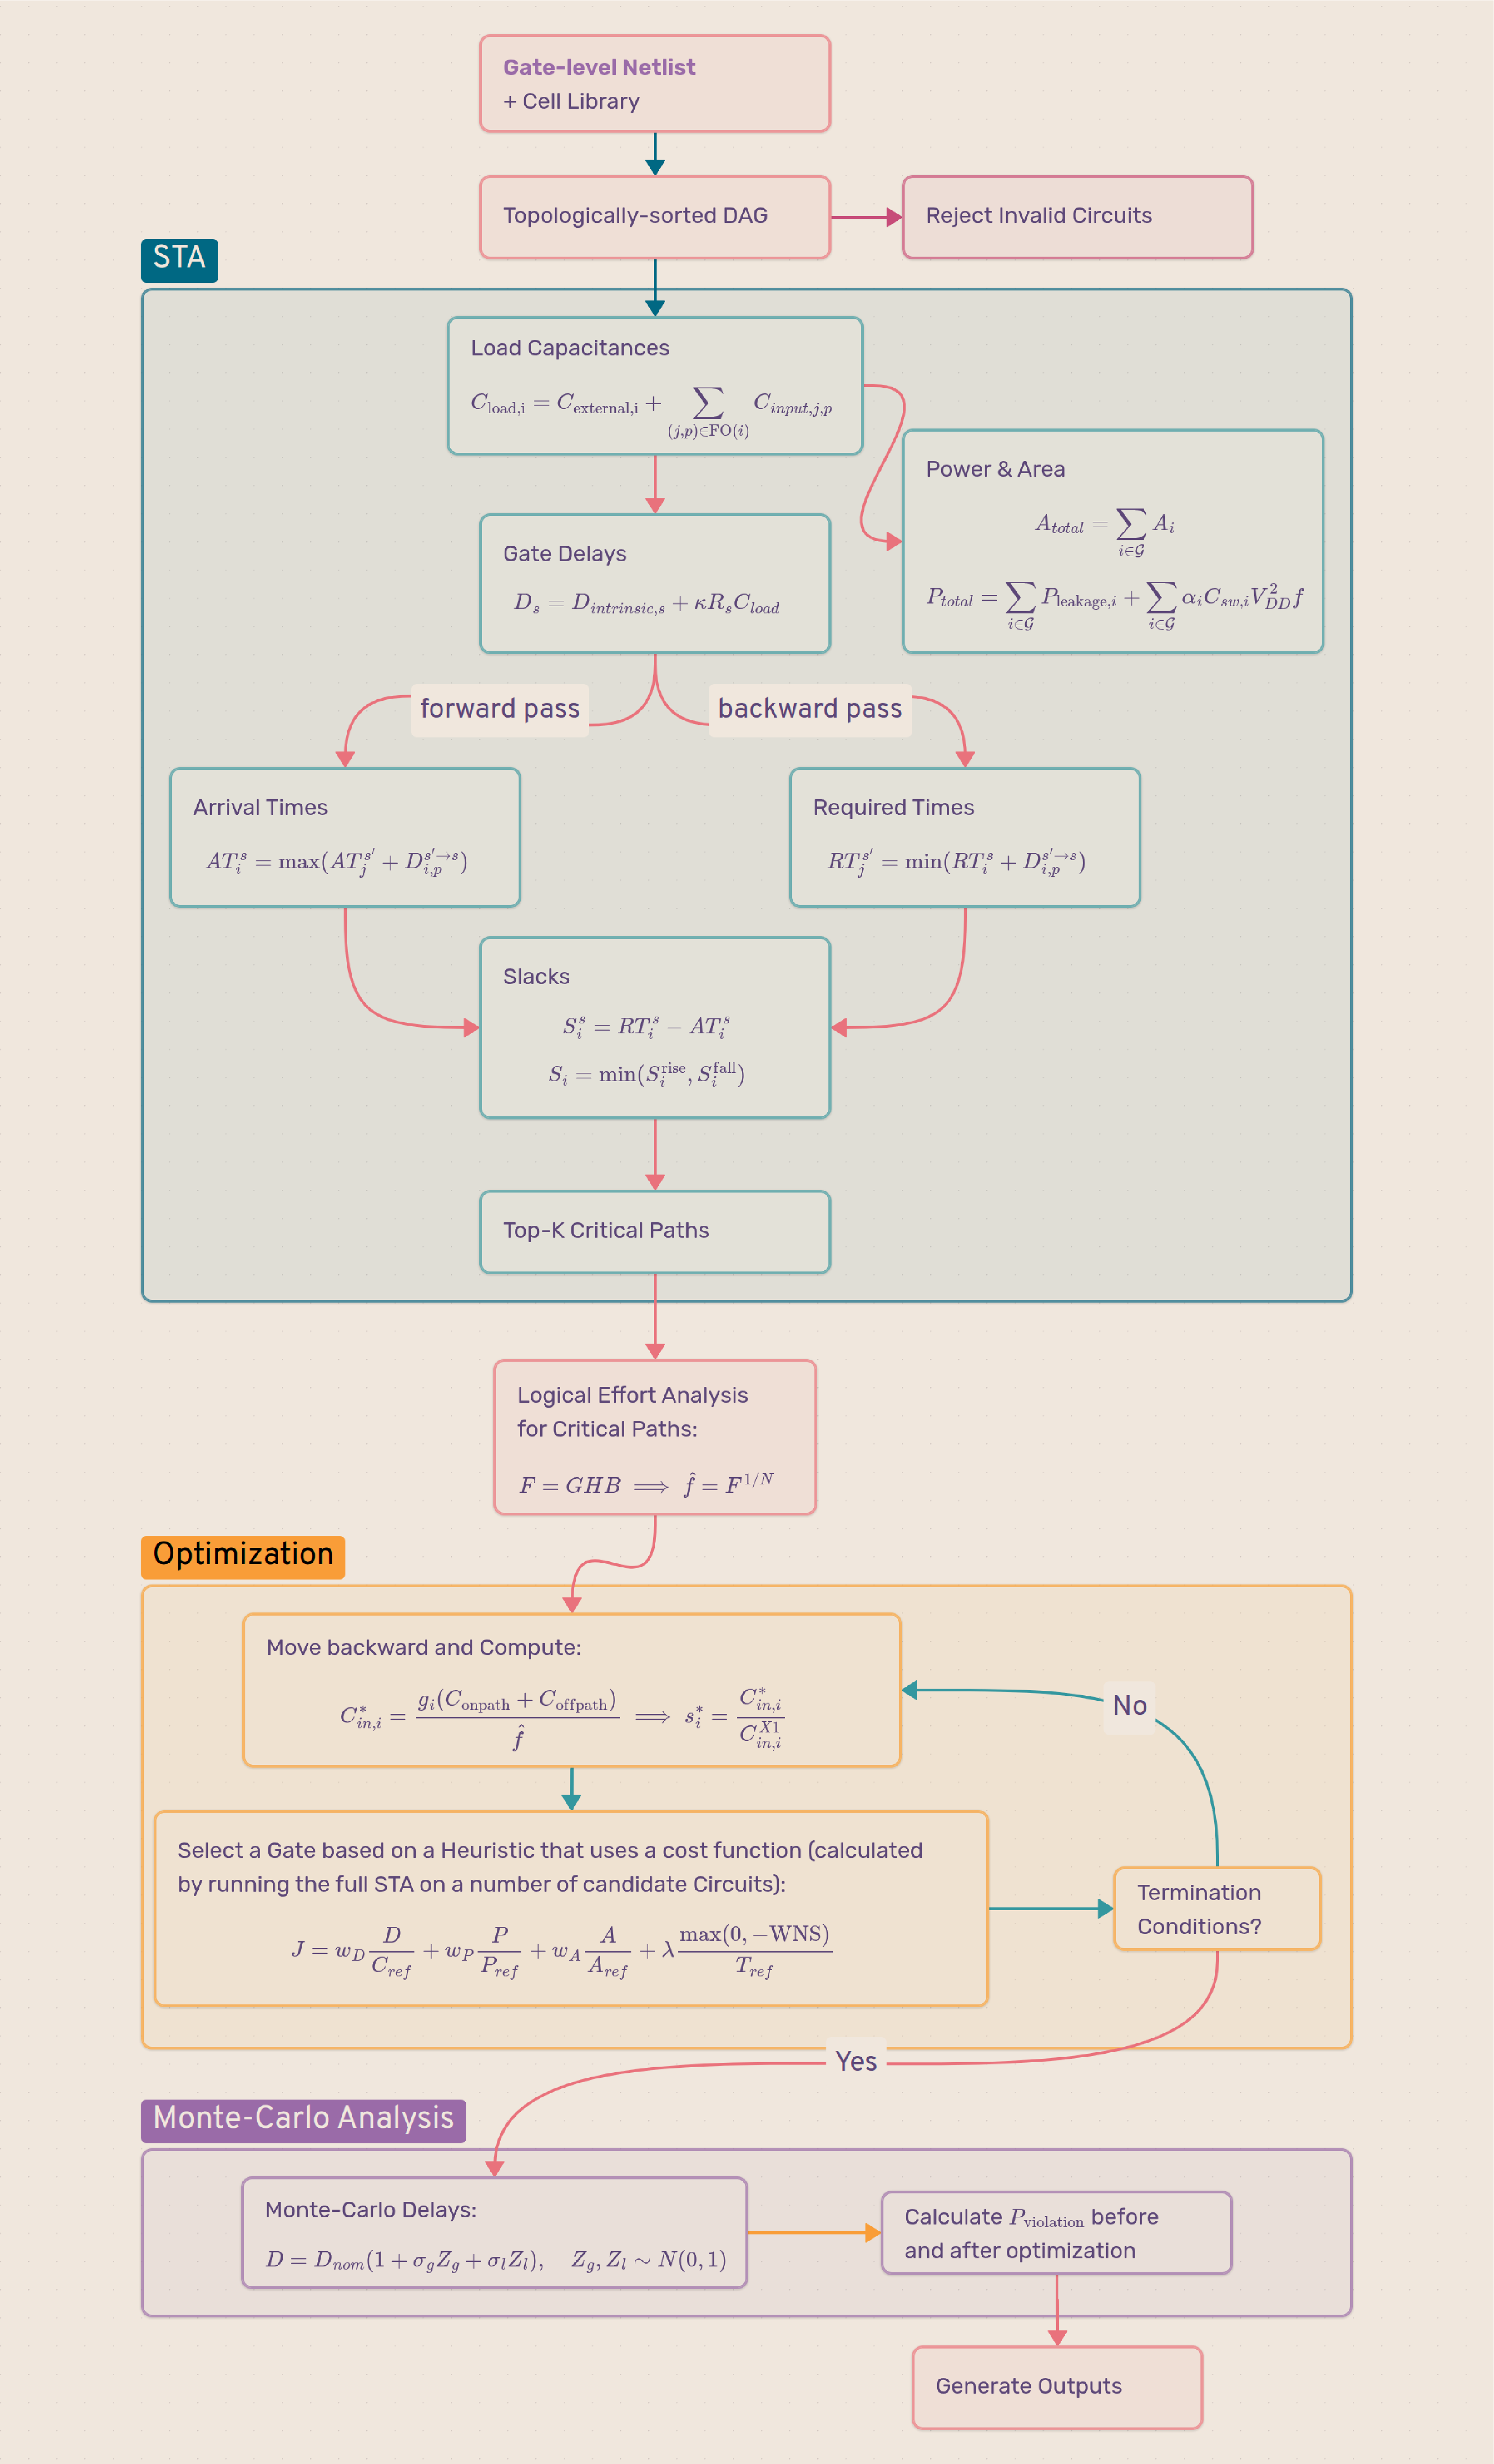
\includegraphics[width=0.97\textwidth]{Architecture}
    \caption{End-to-end data flow of the analyzer, from input files to
    reported outputs.}
    \label{fig:dataflow}
\end{figure}

\section{Command-Line Interface and Output Contract}
\label{sec:arch-cli}

The command-line entry point is \code{app/cli.py:main(argv)}, which builds
its parser via \code{build\_argument\_parser()} and delegates to
\code{app/application.py:run\_application(argv)}. That function performs,
in order: \code{setup\_logging(verbose, log\_path)}; input loading via
\code{load\_circuit(arguments)} (which internally parses the configuration,
cell library, and netlist, and constructs the initial \code{Circuit}); and,
if loading succeeds, \code{run\_experiments(circuit, netlist\_path,
output\_dir)}, which constructs an \code{Experiments} instance
(\cref{sec:arch-dataflow}) and calls its \code{run(circuit)} method. A
single circuit is analyzed with:

\begin{lstlisting}[language=bash, style=pythonstyle, numbers=none]
./run_circuit.sh c01_inverter_chain
\end{lstlisting}

which writes an independent, self-contained directory
\code{outputs/c01\_inverter\_chain/} containing every artifact listed in
\cref{tab:output-contract}. Invalid inputs produce only
\code{validation\_report .json} and \code{run.log}, and the process exits
with a nonzero status without attempting any timing analysis, so that a
downstream script (or the batch mode, \code{run\_circuit.sh --all}) can
mechanically distinguish an analyzed circuit from a rejected one.

\begin{longtable}{@{}p{0.34\textwidth}p{0.60\textwidth}@{}}
\toprule
\textbf{Artifact} & \textbf{Contents} \\
\midrule
\endhead
\code{validation\_report.json}, \code{run.log} &
  Structured input-validation result and the complete execution log. \\[3pt]
\code{fanout\_capacitances.csv}, \code{gate\_delays.csv} &
  One row per gate, topologically ordered: output load and rise/fall
  delay. \\[3pt]
\code{timing\_analysis.csv} &
  One row per gate: load, rise/fall delay, arrival time, required time,
  transition slack, and overall node slack. \\[3pt]
\code{timing\_summary.csv}, \code{critical\_paths.csv} &
  Circuit delay, WNS, TNS, compliance flag, and the top-$K$ critical
  paths. \\[3pt]
\code{logical\_effort\_paths/ stages/candidates.csv} &
  Path-level ($G,B,H,F,P$), stage-level, and discrete-candidate logical
  effort records. \\[3pt]
\code{optimization\_*.csv}, \code{optimization\_comparison.csv} &
  Complete iteration histories for every heuristic and their head-to-head
  comparison. \\[3pt]
\code{circuit\_graph\_\{pre,post\}\_ optimization.png} &
  Slack-colored circuit diagrams with the critical path highlighted. \\[3pt]
\code{circuit\_topology.json} &
  Versioned graph contract consumed by the interactive viewer
  (\cref{ch:viewer}). \\[3pt]
\code{monte\_carlo\_*.csv}, \code{monte\_carlo\_summary.json} &
  Paired pre-/post-optimization statistical timing results
  (\cref{ch:monte-carlo}), or an explicit ``skipped'' summary when
  disabled. \\[3pt]
\code{summary.json} &
  Aggregate summary for the circuit. \\
\bottomrule
\caption{Output contract produced for every successfully analyzed
circuit.}
\label{tab:output-contract}
\end{longtable}

\newpage
All CSV column names carry explicit units (\code{\_ns}, \code{\_fF},
\code{\_uW}); all numeric computation and serialization retain full
floating-point precision, with rounding applied only when a value is
formatted for a plot label, so that downstream tooling never operates on
already-rounded intermediate values.


\chapter{Input Parsing and Validation}
\label{ch:validation}

\section{Netlist and Cell Library Grammar}
\label{sec:val-grammar}

The netlist format is a flat, line-oriented text grammar with three
statement forms, one per line, blank lines and \code{\#}-prefixed comments
ignored:

\begin{lstlisting}[language=bash, style=pythonstyle, numbers=none]
INPUT  <signal_name>
OUTPUT <signal_name>
<instance_name> <cell_name> <input_net_1> ... <input_net_N> <output_net>
\end{lstlisting}

The standard-cell library is a single JSON file, shared across every
circuit, describing thirty-six cells across twelve logic families
(\code{INV}, \code{BUF}, \code{AND2}, \code{NAND2}, \code{OR2}, \code{NOR2},
\code{XOR2}, \code{XNOR2}, three-input variants, and so on), each available
in three drive-strength sizes (\code{X1}, \code{X2}, \code{X4}). Every cell
entry supplies, per input pin, its capacitance, logical effort, and timing
sense (\cref{sec:bg-unate}), and, per cell, its intrinsic rise/fall delay,
rise/fall output resistance, internal capacitance, normalized parasitic
delay, leakage power, and area --- i.e.\ every quantity that appears on the
right-hand side of \cref{eq:cload,eq:drise,eq:dfall,eq:le-stage,eq:power-area,eq:power-total}.

\section{Configuration Schema}
\label{sec:val-config}

The configuration file supplies every circuit- and run-specific parameter
that is not part of the netlist or the (shared) cell library: primary-input
arrival times, primary-output required times and external loads, operating
conditions (supply voltage, clock frequency, temperature, switching
activity factors), area and power budgets, optimizer settings (allowed
sizes, iteration limit, cost weights), and Monte Carlo settings (sample
count, variation strengths, random seed). Every field is validated for
presence, type, and range before any analysis is attempted; a missing or
malformed field is rejected with a specific error message rather than
silently substituted with a default, on the reasoning that a silently
wrong configuration value is more dangerous than a loud rejection.

\section{Structural Validation Stages}
\label{sec:val-stages}

Validation proceeds through four ordered stages, and the process is
aborted at the first stage that fails so that no analysis is ever attempted
on an input the tool cannot trust.

\begin{enumerate}
    \item \textbf{Configuration.} Schema and range validation as described
          above.
    \item \textbf{Cell library.} Schema validation of the shared library
          file (every cell has a complete, correctly typed set of the
          fields listed in \cref{sec:val-grammar}).
    \item \textbf{Netlist.} Parses the grammar and performs every
          netlist-level structural check listed in \cref{tab:error-classes}.
    \item \textbf{DAG.} Builds the circuit graph and topologically sorts it;
          failure at this stage means a combinational (feedback) loop was
          detected.
\end{enumerate}

\subsection{Combinational Loop Detection}
\label{sec:val-cycle}

A combinational loop cannot be resolved by a linear topological ordering:
Kahn's algorithm repeatedly removes vertices with zero remaining in-degree
and terminates having placed every vertex if and only if the graph is
acyclic. If any vertices remain unplaced when the algorithm's queue empties,
those vertices participate in (or exclusively depend on) a cycle, and the
netlist is rejected with the specific set of implicated gate instances
reported to the user.

\section{Error Taxonomy and the Invalid-Circuit Benchmark Set}
\label{sec:val-errors}

Six structural error classes are validated against, matching the six
invalid benchmark circuits supplied with the assignment
(\code{e01}--\code{e06}). \Cref{tab:error-classes} summarizes each class,
the pipeline stage at which it is detected, and the diagnostic message
format produced.

\begin{longtable}{@{}p{0.25\textwidth}p{0.10\textwidth}p{0.5\textwidth}@{}}
\toprule
\textbf{Error class} & \textbf{Stage} & \textbf{Detection} \\
\midrule
\endhead
\code{undefined\_cell} &
  Netlist &
  A gate instance references a cell name absent from the library. \\[4pt]
\code{undriven\_signal} &
  Netlist &
  A gate input net is neither a primary input nor the output of any gate
  in the netlist. \\[4pt]
\code{multiple\_drivers} &
  Netlist &
  A net name appears as the output of more than one gate instance (or of
  both a gate and a declared primary input). \\[4pt]
\code{invalid\_input\_count} &
  Netlist &
  The number of input nets listed for a gate instance does not match the
  defined cell's number of input pins. \\[4pt]
\code{undriven\_output} &
  Netlist &
  A signal declared with \code{OUTPUT} is not the output of any gate
  instance. \\[4pt]
\code{combinational\_loop} &
  DAG &
  Topological sort fails to place every gate (\cref{sec:val-cycle}). \\
\bottomrule
\caption{Structural error taxonomy.}
\label{tab:error-classes}
\end{longtable}


\chapter{Static Timing Analysis Engine}
\label{ch:sta}

This chapter documents the implementation of the theory reviewed in
\cref{sec:bg-sta}, as it appears in \code{analysis/sta.py}. The module's
only two public entry points are

\begin{lstlisting}[style=pythonstyle, numbers=none]
def analyze_timing(circuit: Circuit,
                   gate_delays: Mapping[str, RiseFall] | None = None
                   ) -> TimingAnalysisResult: ...

def analyze_timing_metrics(circuit: Circuit,
                   gate_delays: Mapping[str, RiseFall] | None = None
                   ) -> TimingMetrics: ...
\end{lstlisting}

\code{analyze\_timing} is the full analysis used everywhere in this report
(\cref{ch:results}) and returns a \code{TimingAnalysisResult} --- a frozen
dataclass carrying \code{critical\_paths}, \code{wns}, \code{tns},
\code{circuit\_delay}, and the full \code{arrival\_times} /
\code{required\_times} / \code{transition\_slacks} tables (each a mapping
from net name to a \code{RiseFall} pair), plus a
\code{node\_slack(net\_name)} convenience method.
\code{analyze\_timing\_metrics} is a deliberately cheaper sibling, used by
the optimizer's inner evaluation loop (\cref{sec:opt-eval}) whenever the
full critical-path list is not needed for a particular candidate check. Its
speedup is not merely skipping the reporting of unneeded data: since
$\mathrm{WNS}$/$\mathrm{TNS}$ (\cref{eq:wns-tns}) only ever need each
primary output's \emph{own} configured required time
(\code{circuit.config.output\_required(net\_name)}) compared against that
output's forward-computed arrival time, \code{analyze\_timing\_metrics}
never performs the full backward propagation of \cref{eq:backward-sta}
through the circuit's internal nodes at all --- it calls only the lean
arrival-time pipeline (\code{\_compute\_arrival\_values} /
\code{\_maximum\_gate\_arrival}, \cref{sec:sta-forward}), which does not
even retain the tie-tracking predecessor information \code{analyze\_timing}
needs for path reconstruction, and computes each output's slack directly
against its own configured requirement.

Both public functions accept an optional \code{gate\_delays} override,
which the Monte Carlo module (\cref{ch:monte-carlo}) uses to inject a
sample's perturbed delay set without needing a variant analysis path of its
own. Internally, both are thin wrappers around a shared private pipeline in
\code{analysis/sta.py}, whose exact signatures are reproduced below since
they pin down what state flows between the forward pass, the
backward pass, and path extraction:

\begin{lstlisting}[style=pythonstyle, numbers=none]
def _run_sta(circuit: Circuit, gate_delays: Mapping[str, RiseFall]
             ) -> tuple[dict[str, RiseFall],   # arrival_times
                        dict[str, RiseFall],   # required_times
                        PredecessorTable,      # controlling arcs
                        dict[str, RiseFall]]:  # transition_slacks

def _compute_arrival_times(circuit, gate_delays
    ) -> tuple[dict[str, RiseFall], PredecessorTable]: ...   # Sec. 5.3
def _compute_required_times(circuit, gate_delays) -> dict[str, RiseFall]: ...     # Sec. 5.4
def _compute_transition_slacks(arrival_times, required_times
        ) -> dict[str, RiseFall]: ...                    # Sec. 5.5
def _find_critical_paths(circuit, predecessors, transition_slacks
        ) -> list[CriticalPath]: ...                     # Sec. 5.6
def _trace_paths_backward(circuit, current_net, current_transition,
        output_net, reversed_steps, reversed_transitions, endpoint_slack, found_paths, predecessors) -> None: ...    # Sec. 5.6
\end{lstlisting}

with \code{\_compute\_circuit\_delay} and \code{\_compute\_output\_slack\_metrics}
deriving \code{circuit \_delay}, \code{wns}, and \code{tns} from the
completed arrival/slack tables, and \code{\_timing\_result} assembling the
final \code{TimingAnalysisResult}. The type
\code{PredecessorTable = Mapping[tuple[str, Transition],
tuple[PredecessorArc, ...]]} is itself worth noting: it is keyed by
\emph{every} (net, transition) pair to a \emph{tuple} of controlling
predecessor arcs, not a single one --- this is precisely the data structure
that makes exhaustive tie recording (\cref{sec:sta-forward}) possible,
since \code{\_compute\_arrival\_times} records every arc attaining the
maximum in \cref{eq:forward-sta}, and \code{\_trace\_paths\_backward}
later branches over exactly that stored tuple rather than recomputing or
re-deciding predecessor selection from scratch.

The engine executes in five ordered steps for a given, fixed gate-sizing
assignment: (1) load and delay computation (\cref{sec:sta-load}), performed
eagerly by \code{Circuit.\_\_init\_\_} itself rather than by
\code{analyze\_timing} (\cref{sec:arch-principles}); (2) forward propagation
(\cref{sec:sta-forward}); (3) backward propagation
(\cref{sec:sta-backward}); (4) slack, WNS, and TNS computation
(\cref{sec:sta-slack}); and (5) critical-path extraction
(\cref{sec:sta-paths}). Steps (2) and (3) both consume the results of step
(1) but not of each other, and are logically independent of one another
aside from that shared dependency.

\section{Circuit Graph Construction and Topological Order}
\label{sec:sta-graph}

Once a netlist has passed validation (\cref{ch:validation}), it is
represented as an object graph rather than a collection of string-indexed
lookup tables: each net object holds a direct reference to the gate object
that drives it and a list of the \code{(pin\_index, gate)} pairs it loads,
and each gate object holds direct references to its input net objects and
its output net object. This means that finding ``who drives net $X$'' or
``what does gate $Y$ fan out to'' is an $O(1)$ pointer dereference rather
than a linear scan over every gate in the circuit, which matters
materially at the scale of the optimizer's inner loop
(\cref{ch:optimization}), where the same queries are issued on the order of
hundreds of times per circuit.

The topological order is computed once, at \code{Circuit} construction, by
the module-level helper \code{\_make\_topological\_order(netlist, gates) ->
tuple[tuple[Gate, ...], ...]} (\code{domain/circuit.py}) using Kahn's
algorithm, and is stored not as a flat list but as a sequence of
\emph{levels} --- exactly the nested-tuple return type above: gates are
grouped by their longest-path depth from any
primary input, so that all gates in level $\ell$ depend only on gates in
levels $0, \ldots, \ell-1$, and this is the \code{topological\_order}
field consumed directly by \code{\_compute\_arrival\_times}'s outer
\code{for level in circuit.topological\_order:\allowbreak\ for gate in
level:} loop (\cref{sec:sta-forward}). Flattening the levels in order recovers an
ordinary topological order; the level structure itself is not required for
correctness of the forward/backward passes below (which only need \emph{a}
topological order, not a minimal-depth one), but is retained because it is
useful metadata for the benchmark generator's stratification by circuit
depth (\cref{ch:benchmarking}).

\section{Load and Delay Computation}
\label{sec:sta-load}

\Cref{eq:cload,eq:drise,eq:dfall} are evaluated for every gate in a single
pass, independent of iteration order, since both quantities depend only on
the currently-assigned cell sizes of a gate and its fan-out --- never on an
arrival or required time. Concretely, this computation lives entirely in
\code{domain/circuit.py} and runs once, eagerly, inside
\code{Circuit.\_\_init\_\_}, via two private methods:

\begin{lstlisting}[style=pythonstyle, numbers=none]
def _compute_fanout_capacitances(self) -> dict[str, float]: ...
    # Eq. (2.1)
def _compute_gate_delays(self) -> dict[str, RiseFall]: ...
    # Eq. (2.2)-(2.3)
\end{lstlisting}

with the per-gate rise/fall delay itself computed by the module-level
helper \code{\_gate\_delay( cell: Cell, load\_capacitance: float, kappa:
float) -> RiseFall}, and total area and power by
\code{Circuit.\_compute\_area()} and \code{Circuit.\_compute\_power()}
(\cref{ch:power-area}). This is a common point of confusion worth stating
explicitly: delay is \emph{not} recomputed as a function of arrival
time during the forward pass; it is a fixed property of the current sizing
assignment, computed once by \code{Circuit.\_\_init\_\_} and only ever
\emph{read} by \code{analysis/sta.py}, never recomputed there.

\section{Forward Propagation}
\label{sec:sta-forward}

\Cref{eq:forward-sta} is evaluated for every gate in topological order by
\code{\_compute\_arrival\_times} (\cref{sec:sta-graph}), which delegates
the per-gate, per-transition maximization to
\code{\_select\_pred \newline ecessors(circuit, gate, output\_transition,
arrival\_times, gate\_delays) ->\newline tuple[float, tuple[PredecessorArc, ...]]}.
Two implementation details, both visible directly in this function's body,
are worth making explicit.

\paragraph{Net-keyed timing tables.} Arrival times are stored in a single
\code{dict[str, RiseFall]} keyed by \emph{net} name, not by gate name. A
primary input's net and a gate's output net are both, from this table's
point of view, just nets with an associated
$(\mathrm{AT}^{\mathrm{rise}}, \mathrm{AT}^{\mathrm{fall}})$
pair; primary-input nets have theirs supplied directly from
\code{circuit.config.input\_arrival(net \_name)}, while gate-output nets have
theirs computed by \cref{eq:forward-sta}. This avoids the need for a
downstream consumer of an arrival time to first determine ``is this a
primary input or a gate output'' before looking it up.

\paragraph{Exhaustive tie recording.} \code{\_select\_predecessors} builds a
list of every \code{(candidate\_arrival, (pin\_number,
input\_transition))} pair across a gate's input pins and their legal input
transitions (\code{\_valid\_input\_transitions}, implementing
\cref{sec:bg-unate}), takes \code{maximum\_arrival = max(...)}, and returns
\emph{every} candidate whose arrival exactly equals that maximum as a tuple
of \code{PredecessorArc}s --- not merely the first one encountered. This
matters directly for critical-path reconstruction (\cref{sec:sta-paths}): a
circuit with a genuinely symmetric or reconvergent structure can have two
structurally distinct paths that are exactly equally critical, and
discarding all but one of them arbitrarily would silently under-report the
set of paths actually responsible for the reported worst-case delay.

\section{Backward Propagation}
\label{sec:sta-backward}

\Cref{eq:backward-sta} is evaluated for every gate in \emph{reverse}
topological order by \code{\_compute\_required \_times}, seeded at the
primary outputs with \code{circuit.config.output\_required(net\_name)}. The
propagation of a single required time backward through one timing arc is
isolated into its own pure function,

\begin{lstlisting}[style=pythonstyle, numbers=none]
def _propagate_required(output_required: RiseFall, gate_delay: RiseFall,
                        timing_sense: TimingSense) -> RiseFall: ...
\end{lstlisting}

whose three branches implement \cref{sec:bg-unate}'s three timing-sense
cases directly: positive-unate subtracts $D_i^{s}$ from
$\mathrm{RT}_i^{s}$ transition-for-transition; negative-unate does the same
with rise and fall swapped; and, for a non-unate pin, both output
transitions are legal regardless of which input transition is being
evaluated, so the function computes
\code{earliest\_candidate = min(output\_required.rise - gate\_delay.rise,
output\_required.fall - gate\_d\newline elay.fall)} once and returns it as
\emph{both} the rise and fall required time propagated through that pin --- a
conservative choice that is required for correctness, since a non-unate
input transition's required time must respect whichever output transition
it might actually cause. \code{\_compute\_required\_times} then folds this
per-arc result into the running required time of each input net via a
plain \code{min(...)}, implementing the outer minimization of
\cref{eq:backward-sta} over every fan-out arc.

\section{Slack, WNS, and TNS}
\label{sec:sta-slack}

\Cref{eq:slack,eq:wns-tns} are evaluated by
\code{\_compute\_transition\_slacks} and
\code{\_compute\_o\newline utput\_slack\_metrics} directly from the arrival- and
required-time tables produced above. A configuration flag,
\code{config.timing\_analysis.separate\_rise\_fall}
(\code{TimingAnalysisConfig}, \cref{tab:arch-domain-api}), read inside
\code{\_output\_slack\_values}, controls whether rise and fall slack at a given
primary output are treated as two independent entries in the WNS/TNS
computation (the default, and the behavior implied by a literal reading of
\cref{eq:wns-tns}) or collapsed to a single per-output worst-case value
first; this is useful when a downstream consumer only cares
about the offending net, not which polarity of transition is responsible.

\section{Critical-Path Extraction}
\label{sec:sta-paths}

A na\"ive definition of ``the $K$ worst paths'' as ``the $K$ worst
(endpoint, transition) pairs, each with one arbitrarily chosen predecessor
chain'' would silently under-represent circuits with tied critical paths.
Path extraction is instead implemented by \code{\_find\_critical\_paths},
which iterates every primary-output net and both of its transitions and
calls the recursive helper:

\begin{lstlisting}[style=pythonstyle, numbers=none]
def _trace_paths_backward(circuit, current_net, current_transition,
        output_net, reversed_steps, reversed_transitions, endpoint_slack, found_paths, predecessors) -> None: ...
\end{lstlisting}

which \emph{branches} at every tie recorded by \code{\_select\_predecessors}
(\cref{sec:sta-forward}): it looks up \code{predecessors[(current\_net.name,
current\_transition)]}, and recurses once per stored \code{PredecessorArc}
in that tuple, prepending a \code{PathStep(gate, input\_pin)} to
\code{rever\newline sed\_steps} each time, until \code{current\_net.net\_type is
NetType.INPUT}, at which point a complete \code{CriticalPath(path, transitions,
slack)} is appended to \code{found\_paths}. All paths produced by this
search, across all endpoints, are pooled into a single list, sorted by
\code{path.slack}, and truncated to
\code{circuit.config.timing\_analysis.top\_k\_paths} by
\code{\_find\_critical\_paths} itself. Two consequences of this design are
worth stating explicitly, since they differ from a simpler ``one path per
worst endpoint'' scheme: first, the reported top-$K$ list is not guaranteed
to contain one path per distinct endpoint --- a circuit with several tied
routings to the same endpoint can occupy multiple slots in the list; second,
this is a strictly more complete answer to ``which paths are responsible
for the worst delay'' than an implementation that picks one arbitrary
routing per endpoint, at the cost of a somewhat less predictable
relationship between $K$ and the number of distinct endpoints represented.

\section{Worked Example: \texttt{c01\_inverter\_chain}}
\label{sec:sta-worked-example}

To ground the equations of this chapter in concrete numbers, this section
traces the engine's computation by hand on the smallest supplied benchmark
circuit, a three-gate inverter--buffer--inverter chain:

\begin{lstlisting}[language=bash, style=pythonstyle, numbers=none]
INPUT A
G1 INV_X1 A  N1
G2 BUF_X1 N1 N2
G3 INV_X1 N2 OUT
OUTPUT OUT
\end{lstlisting}

with primary-input arrival times $\mathrm{AT}_A^{\mathrm{rise}} =
\mathrm{AT}_A^{\mathrm{fall}} = 0$~ns, primary-output required times
$\mathrm{RT}_{\mathrm{OUT}}^{\mathrm{rise}} =
\mathrm{RT}_{\mathrm{OUT}}^{\mathrm{fall}} = 0.11$~ns, and an external load
of $4.0$~fF on \code{OUT}. \Cref{tab:c01-worked} reproduces, gate by gate,
the load, delay, arrival time, required time, and slack computed by
\cref{eq:cload,eq:drise,eq:dfall,eq:forward-sta,eq:backward-sta,eq:slack}
using the \code{INV\_X1}/\code{BUF\_X1} library entries. The resulting
$\mathrm{WNS} = 0.009$~ns and $\mathrm{TNS} = 0$~ns (no violation) were
confirmed to match the tool's reported output to six decimal places.

\begin{table}[H]
\centering
\small
\begin{tabular}{@{}lccccc@{}}
\toprule
\textbf{Gate} & \textbf{$C_{\mathrm{load}}$ (fF)} & \textbf{$D_{\mathrm{rise}}/D_{\mathrm{fall}}$ (ns)} & \textbf{$\mathrm{AT}^{\mathrm{rise}}/\mathrm{AT}^{\mathrm{fall}}$} & \textbf{$\mathrm{RT}^{\mathrm{rise}}/\mathrm{RT}^{\mathrm{fall}}$} & \textbf{Slack (ns)} \\
\midrule
G1 (\code{INV\_X1}) & 1.0 & 0.0240 / 0.0185 & 0.0240 / 0.0185 & 0.0350 / 0.0275 & 0.011 / 0.009 \\
G2 (\code{BUF\_X1}) & 1.0 & 0.0370 / 0.0315 & 0.0610 / 0.0500 & 0.0720 / 0.0590 & 0.011 / 0.009 \\
G3 (\code{INV\_X1}) & 4.0 & 0.0510 / 0.0380 & 0.1010 / 0.0990 & 0.1100 / 0.1100 & 0.009 / 0.011 \\
\bottomrule
\end{tabular}
\caption{Hand-verified static timing analysis of
\texttt{c01\_inverter\_chain}. G3 is the sole primary-output-driving gate;
its rise slack of \SI{0.009}{ns} equals the circuit-level WNS.}
\label{tab:c01-worked}
\end{table}

Two points are worth drawing attention to that a reader might otherwise
gloss over. First, because \code{INV\_X1} is negative-unate, G1's rise
\emph{output} arrival time is driven by the primary input's \emph{fall}
transition ($\mathrm{AT}_A^{\mathrm{fall}} = 0 \Rightarrow
\mathrm{AT}_{G1}^{\mathrm{rise}} = 0 + D_{\mathrm{rise},G1} = 0.024$), not
its rise transition; a reader tracing the table without accounting for
timing sense would expect the opposite pairing. Second, the worst slack in
the circuit (\SI{0.009}{ns}) alternates which transition it belongs to at
every stage of the chain ($\mathrm{fall}$ at G1, $\mathrm{fall}$ at G2,
$\mathrm{rise}$ at G3) precisely because of this same negative-unate
alternation --- a further illustration of why rise and fall must be
propagated as genuinely independent quantities rather than a single
worst-case delay per gate.

\chapter{Logical-Effort Analysis}
\label{ch:logical-effort}

This chapter documents the implementation of \cref{sec:bg-le} as applied to
the top-$K$ critical paths reported by the STA engine
(\cref{sec:sta-paths}). Logical-effort analysis is purely a
\emph{post-processing} view over the STA result: it reads capacitances and
delays directly off the already-analyzed circuit and does not perform any
independent simulation of its own, so its results are always consistent
with whatever sizing assignment was current when the STA pass that produced
the critical paths was run.

\section{Per-Stage Effort Computation}
\label{sec:le-stage}

For each critical path, the sequence of gates from the driving primary
input to the endpoint is walked in order. At each stage $i$, the specific
input pin through which the path enters that gate is identified (recovered
from the same predecessor information used to reconstruct the path in
\cref{sec:sta-paths}), which determines $g_i$, the logical effort of that
particular pin, from the cell library. The on-path receiver capacitance
$C_{\mathrm{onpath},i}$ is the input pin capacitance of the next stage along
the path (or, for the final stage, the external load applied to the
endpoint's net); the off-path capacitance $C_{\mathrm{offpath},i}$ is
obtained by subtracting $C_{\mathrm{onpath},i}$ from the gate's total output
load $C_{\mathrm{load},i}$, which was already computed by the STA engine
(\cref{eq:cload}) and reflects the gate's \emph{actual, current} fan-out ---
not an idealized or path-only load. Branching effort $b_i$, electrical
effort $h_i$, and stage effort $f_i$ then follow directly from
\cref{eq:le-stage}.

\section{Path-Level Effort and the Sizing Target}
\label{sec:le-path}

Path-level quantities $G$, $B$, $H$, $F$, and $P$
(\cref{eq:le-path}) are accumulated across all stages of the path, and the
optimal per-stage effort $\hat f = F^{1/N}$ and theoretical minimum path
delay $D_{LE,\mathrm{min}}$ (\cref{eq:le-min-delay}) are computed once per
path. Every stage's actual effort $f_i$ is then compared to $\hat f$: a
stage with $f_i \gg \hat f$ is disproportionately loaded relative to its own
drive strength and is, by the theory, the best next candidate for
up-sizing. This overshoot quantity, $f_i - \hat f$, is the ranking signal
consumed by the optimizer's logical-effort-guided heuristics
(\cref{sec:opt-heuristics}).

Because each stage's desired capacitance (\cref{eq:le-target-cap}) depends
only on that stage's own current load $C_{\mathrm{total},i}$ and its own
$g_i$ --- both already known from the current, fixed sizing assignment ---
computing every stage's target capacitance does not require processing the
path in any particular order; the ``move backward along the path'' framing
used in the assignment specification is a presentational convenience,
carried over unchanged from classical hand-calculation logical-effort
sizing, rather than a genuine data dependency in this implementation.

\section{Discrete Sizing Candidates}
\label{sec:le-candidates}

The continuous target capacitance $C^{*}_{\mathrm{in},i}$
(\cref{eq:le-target-cap}) will almost never coincide exactly with one of the
three discrete sizes (\code{X1}/\code{X2}/\code{X4}) available in the
library. Rather than rounding to the single nearest size by absolute
capacitance difference, the implementation \emph{brackets} the target: it
finds the largest available cell whose input pin capacitance is still at or
below the target, and the smallest available cell whose input pin
capacitance is at or above it, and reports both as candidates (falling back
to the nearest boundary cell if the target lies outside the family's
achievable range entirely). This bracketing approach is more principled
than nearest-distance rounding because it guarantees the two candidates
straddle the theoretical ideal from both sides, which matters when the
optimizer (\cref{ch:optimization}) evaluates both bracket candidates via a
full STA re-run and lets the \emph{measured} outcome, not the continuous
approximation, determine which one is actually better once real,
non-idealized loading effects on neighboring gates are accounted for.

\begin{table}[H]
\centering
\small
\begin{tabular}{@{}lcccc@{}}
\toprule
\textbf{Quantity} & \textbf{Symbol} & \textbf{Meaning} & \textbf{Computed from} \\
\midrule
Logical effort & $g_i$ & Gate-topology cost of driving equal load & Library, per pin \\
Electrical effort & $h_i$ & On-path fan-out ratio & \cref{eq:le-stage} \\
Branching effort & $b_i$ & Off-path loading tax & \cref{eq:le-stage} \\
Stage effort & $f_i$ & $g_i b_i h_i$ & \cref{eq:le-stage} \\
Path effort & $F$ & $\prod_i f_i$ & \cref{eq:le-path} \\
Optimal stage effort & $\hat f$ & $F^{1/N}$ & \cref{eq:le-min-delay} \\
Theoretical min.\ delay & $D_{LE,\mathrm{min}}$ & $\tau(NF^{1/N}+P)$ & \cref{eq:le-min-delay} \\
Target capacitance & $C^{*}_{\mathrm{in},i}$ & Ideal input cap.\ for stage $i$ & \cref{eq:le-target-cap} \\
\bottomrule
\end{tabular}
\caption{Summary of quantities reported per stage/path in
\texttt{logical\_effort\_paths.csv}, \texttt{logical\_effort\_stages.csv},
and \texttt{logical\_effort\_candidates.csv}.}
\label{tab:le-summary}
\end{table}

\chapter{Power and Area Estimation}
\label{ch:power-area}

Power and area are recomputed, in full, after every accepted change to the
circuit's sizing assignment, so that the
optimizer's cost function always operates on the
current totals.

\section{Static (Leakage) Power}
\label{sec:pa-leakage}

Leakage power is supplied directly, per cell, by the standard-cell library
and is independent of switching activity or circuit state; total leakage is
the direct sum given in \cref{eq:power-total}. It depends only on which
cells are currently assigned, and therefore changes only when a gate is
resized.

\section{Dynamic Power}
\label{sec:pa-dynamic}

Dynamic power follows the activity-factor model of \cref{eq:power-area}. The
switching activity factor $\alpha_i$ for a given net is read from the
configuration file's per-net override table if present, and otherwise
falls back to a single circuit-wide default activity factor, also supplied
by the configuration. The effective switched capacitance
$C_{\mathrm{sw},i}$ combines the gate's output load $C_{\mathrm{load},i}$
--- already computed by the STA engine (\cref{eq:cload}) and therefore
automatically reflecting the gate's current fan-out --- with its internal
capacitance, a library-supplied constant per cell that accounts for
switching energy dissipated inside the gate itself, independent of external
loading.

\section{Area}
\label{sec:pa-area}

Total area is the direct sum of the currently-assigned cell's area over
every gate, as in \cref{eq:power-area}. Because larger-drive-strength cells
in the library are strictly larger in area (and generally larger in both
leakage and internal capacitance) than their smaller-drive-strength
counterparts within the same family, every accepted up-sizing decision made
by the optimizer (\cref{ch:optimization}) has an unconditional, nonzero
cost in both area and power, regardless of whether that particular gate
lies on a currently-critical path --- which is precisely why the optimizer
restricts its candidate search to gates that are actually on a reported
critical path (\cref{sec:opt-heuristics}) rather than considering every gate
in the circuit: up-sizing a gate that is not contributing to any timing
violation can only ever worsen the cost function's power and area terms for
no corresponding delay benefit.

\chapter{Gate-Sizing Optimization}
\label{ch:optimization}

The optimizer is implemented in
\code{optimization/optimizer.py:CircuitOptimizer}, with a deliberately
narrow public surface:

\begin{lstlisting}[style=pythonstyle, numbers=none]
class CircuitOptimizer:
    def __init__(self, circuit: Circuit,
                 heuristic: OptimizationHeuristic = BRUTE_FORCE,
                 random_seed: int | None = None) -> None: ...
    def optimize(self) -> OptimizationResult: ...
\end{lstlisting}

Everything else --- candidate generation, cost evaluation, the acceptance
policy, and termination --- is private to this class or to
\code{optimization/heuristics.py}, and is documented in this chapter by
name because the \emph{names} of these private functions are themselves
the clearest statement of the algorithm's structure.

\section{Cost Function}
\label{sec:opt-cost}

Every candidate gate-sizing change is scored by a single normalized cost
function that trades off circuit delay $D_{\mathrm{circuit}}$, total power
$P_{\mathrm{total}}$, total area $A_{\mathrm{total}}$, and any remaining
timing violation, each normalized against the corresponding value of the
\emph{original, unmodified} design (subscript $\mathrm{ref}$), so that the
cost is dimensionless and comparable across circuits of very different
absolute size:

\begin{equation}
    J = w_D \frac{D_{\mathrm{circuit}}}{D_{\mathrm{ref}}}
      + w_P \frac{P_{\mathrm{total}}}{P_{\mathrm{ref}}}
      + w_A \frac{A_{\mathrm{total}}}{A_{\mathrm{ref}}}
      + \lambda\, \frac{\max(0, -\mathrm{WNS})}{T_{\mathrm{ref}}}.
    \label{eq:cost}
\end{equation}

The weights $w_D, w_P, w_A, \lambda$ are read from
\code{Config.optimization.weights} (\code{Optimizati\newline onWeights},
\cref{tab:arch-domain-api}). $D_{\mathrm{ref}}, P_{\mathrm{ref}},
A_{\mathrm{ref}}$ are captured exactly once by the static method
\code{CircuitOptimizer.\_normalization\_reference(circuit, timing) ->
\_Normalization Reference}, called only from \code{\_initial\_state()} at
the very start of \code{optimize()}, and never recomputed thereafter, so
that $J$ always measures cost \emph{relative to the starting point}.
$T_{\mathrm{ref}}$, a normalizing time reference for the violation penalty,
is taken as the tightest required time among the circuit's primary outputs.

Cost itself is computed by the private method
\code{CircuitOptimizer.\_evaluate(circuit, reference, timing=None) ->
\_Evaluation}, where \code{\_Evaluation} is a frozen dataclass bundling
\code{circuit}, \code{timing}, and \code{cost} together --- the single
value threaded through every other private method below.

\section{Candidate Evaluation}
\label{sec:opt-eval}

Consistent with the immutability principle stated in
\cref{sec:arch-principles}, evaluating a candidate resize never mutates the
circuit currently being optimized.
\code{CircuitOptimizer.\_candidate\_ evaluation(current, reference, gate,
candidate\_cell) -> \_CandidateEvaluation | None} is the single choke
point through which every candidate --- from every heuristic --- passes,
in three ordered steps.

\begin{enumerate}
    \item \textbf{Cheap pre-filter.}
          \code{replacement\_area\_and\_power(current.circuit, gate.name,
          candidate\_cell)} (\cref{tab:arch-domain-api}) computes the
          resulting total area and power \emph{without} constructing a new
          \code{Circuit} object at all. If this alone already exceeds the
          configured budget
          (\code{\_violates\_area\_or\_power\_constraints}), the candidate
          is discarded immediately, before paying for a full circuit
          construction or a timing re-run.
    \item \textbf{Full construction and re-analysis.} Only if the cheap
          check passes is \code{replace\_gate \_cell(current.circuit,
          gate.name, candidate\_cell)} called to build the new, independent
          \code{Circuit} variant, which is then fully re-evaluated:
          \code{\_analyze(circuit)} runs \code{analyze\_timing}
          (incrementing an internal \code{self.\_sta\_calls} counter,
          reported as \code{OptimizationResult.sta\_calls}), and
          \code{\_satisfies\_constraints(circuit)} performs the exact
          (non-delta) area/power check against the fully rebuilt circuit.
    \item \textbf{Cost.} \code{\_evaluate(candidate\_circuit, reference)}
          scores the surviving candidate via \cref{eq:cost}.
\end{enumerate}

If a candidate is not selected, the \code{Circuit} object built for it is
simply discarded --- there is no revert step, because nothing was ever
mutated in place. This is functionally equivalent to an
evaluate-then-revert pattern built on a mutable graph, but structurally
eliminates the possibility of a forgotten or incomplete revert silently
corrupting a subsequent evaluation.

\section{The Acceptance Policy}
\label{sec:opt-accept}

A detail that is easy to miss without reading the source directly, but is
central to how the four heuristics relate to one another: \textbf{there is
exactly one implementation of the two-phase accept/reject policy, and every
heuristic calls it.}

\vspace{10pt}
\begin{lstlisting}[style=pythonstyle, numbers=none]
def _select_next_change(self, current: _Evaluation,
                        candidates: list[_CandidateEvaluation]
                        ) -> _AcceptedChange | _StopDecision: ...
@staticmethod
def _best_timing_change(current, candidates) -> _CandidateEvaluation | None: ...
@staticmethod
def _best_cost_change(candidates) -> _CandidateEvaluation | None: ...
\end{lstlisting}


\newpage \noindent \code{\_select\_next\_change} implements the two-phase rule directly:

\begin{enumerate}
    \item \textbf{While a timing violation remains}
          ($\mathrm{WNS} < 0$, \code{OptimizationPhase.TIMING\_REPAIR}):
          \code{\_best\_timing\_change} selects, among the supplied
          candidates, the one with the lowest cost $J$ among those that
          strictly improve WNS, or, failing that, strictly improve TNS with
          WNS unchanged. If none qualify, \code{\_select\_next\_change}
          returns a \code{\_StopDecision} with termination reason
          \code{NO\_TIMING\_IMPROVEMENT}.
    \item \textbf{Once timing is compliant}
          ($\mathrm{WNS} \geq 0$, \code{OptimizationPhase.COST\_REDUCTION}):
          \code{\_best\_cost\_change} selects the lowest-cost candidate that
          does not reintroduce a violation, and the change is accepted only
          if the resulting cost improvement exceeds
          \code{config.optimization.minimum\_cost\_improvement}. Otherwise, termination reason
          \code{TIMING\_MET\_NO\_COST\_IMPROVEMENT} is returned.
\end{enumerate}

What differs between heuristics is only \emph{how many} candidates
\code{\_select\_next\_change} is called with, and \emph{in what order}
they were generated (\cref{sec:opt-heuristics}) --- not the acceptance
rule itself. Brute force calls it once per iteration with the
\emph{entire} evaluated candidate batch:

\begin{lstlisting}[style=pythonstyle, numbers=none]
choices = tuple(choice_iterator)    # exhaust the whole iterator
candidates = self._candidate_evaluations(current, reference, choices)
return self._select_next_change(current, candidates)  # pick the best of all
\end{lstlisting}

while the other three heuristics instead call
\code{\_evaluate\_single\_choice}, which evaluates exactly \emph{one}
candidate and delegates to the very same function with a singleton list:

\begin{lstlisting}[style=pythonstyle, numbers=none]
def _evaluate_single_choice(self, current, reference, gate, candidate_cell
        ) -> _AcceptedChange | _RejectedChange:
    candidate = self._candidate_evaluation(current, reference, gate, candidate_cell)
    if candidate is None:
        return _RejectedChange(gate.name, candidate_cell.name,
                                "candidate violates area or power constraints")
    decision = self._select_next_change(current, [candidate]) 
    ...
\end{lstlisting}

This makes slack-weighted capacitance, criticality/effort-gap, and random
greedy \emph{sequential, first-improvement} searches: each pulls one
candidate at a time from a pre-ordered stream and immediately accepts or
rejects it, moving to the next candidate in that same stream on rejection,
without re-ranking until a change is actually accepted. Brute force, in
contrast, is a \emph{best-of-batch} search: every eligible candidate is
evaluated fresh each iteration, and the single best one is chosen. The
optimizer's outer loop, \code{optimize()}, regenerates the candidate stream
(\code{choice\_iterator = None}, forcing a fresh call to
\code{\_choice\_iterator} on the next iteration) only \emph{after} an
accepted change, so a rejected candidate does not trigger re-ranking ---
the search simply continues down the same, still-valid-for-the-current-circuit
ordering.

\section{Termination}
\label{sec:opt-termination}

\code{OptimizationTermination} enumerates five possible outcomes, recorded
verbatim in \code{Optim\newline izationResult.termination} and in the
\code{optimization\_*.csv} artifacts: \code{DISABLED} (optimization turned
off in configuration); \code{NO\_TIMING\_IMPROVEMENT} (still violating, no
candidate improves WNS/TNS); \code{NO\_FEASIBLE\_CHANGE} (the candidate
stream is exhausted --- only reachable by the three sequential heuristics,
since brute force always sees its full batch every iteration);
\code{TIMING\_MET\_NO\_COST\_IMPROVEMENT} (compliant, but no candidate
reduces cost enough); and \code{MAXIMUM\_ITERATIONS}.

\section{The Four Sizing Heuristics}
\label{sec:opt-heuristics}

\code{OptimizationHeuristic} (\code{optimization/heuristics.py}) has four
members: \code{BRUTE\_FORCE}, \code{SLACK\_WEIGHTED\_CAPACITANCE},
\code{CRITICALITY\_EFFORT\_GAP}, and \code{RANDOM\_GREEDY}. All four are
dispatched from a single method,
\code{\_choice\_iterator(self, current, random\_gener\newline ator) ->
Iterator[\_SizingChoice]}, whose four branches \emph{are} the precise
definition of what distinguishes the four heuristics: \code{RANDOM\_GREEDY}
takes \code{\_critical\_path\_one\_step\_c\newline hoices(current)} and shuffles it
with \code{random\_generator}; \code{CRITICALITY\_EFFORT\_GAP} passes that
same one-step choice list through
\code{iter\_criticality\_effort\_gap\_choices}; \code{BRUTE\_FORCE} and
\code{SLACK\_WEIGHTED\_CAPACITANCE} both instead start from
\code{\_eligible\_choices(current, allowed\_sizes)}, flattened directly for
brute force or passed through \code{iter\_ranked\_optimi\newline zation\_choices}
for the canonical heuristic.

Two \emph{sources} of candidates are used, and it is important not to
conflate them:

\begin{itemize}
    \item \code{\_critical\_path\_one\_step\_choices(current) ->
          list[tuple[Gate, Cell]]} returns, for every gate on any current
          critical path, only \emph{one} candidate: its immediate
          next-larger cell in the same family (never a logical-effort-derived
          bracket, never a jump of more than one discrete size step).
          \textbf{Both} \code{RANDOM\_GREEDY} \textbf{and}
          \code{CRITICALITY\_EFFORT\_GAP} draw from this same, narrower
          candidate set --- they differ from each other only in the
          \emph{order} they visit it (uniformly shuffled versus
          score-ranked), not in which cells are candidates at all.
    \item \code{\_eligible\_choices(current, allowed\_sizes) ->
          list[OptimizationChoice]} ( where \code{OptimizationChoice =
          tuple[Gate, tuple[Cell, ...]]}) calls
          \code{analysis/ logica\_effort.py:get\_optimization\_candidates},
          which returns, for every gate on any current critical path,
          \emph{every} discrete cell in its logical-effort sizing bracket
          (\cref{sec:le-candidates}) --- potentially more than one size
          step in a single proposal. \textbf{Both} \code{BRUTE\_FORCE}
          \textbf{and} \code{SLACK\_WEIGHTED\_CAPACITANCE} draw from this
          wider, logical-effort-derived candidate set.
\end{itemize}

\subsection{Brute Force}
\label{sec:opt-bruteforce}

Every $(gate, candidate)$ pair in the logical-effort bracket set is
evaluated, in full, every iteration, and \code{\_select\_next\_change}
picks the single best. This is the most thorough of the four heuristics
--- and, per \cref{sec:opt-accept}, the only one that genuinely compares
multiple candidates against each other before choosing, rather than
walking a pre-ordered list --- at the cost of the largest number of full
STA re-runs per accepted change. It is available for manual and diagnostic
use but is not the heuristic invoked to produce the canonical optimized
result reported in \cref{ch:results}.

\subsection{Slack-Weighted Capacitance (Canonical)}
\label{sec:opt-swc}

Draws from the same logical-effort bracket set as brute force, but visits
it as a sequential, first-improvement search, in an order fixed once per
outer-loop iteration by \code{iter\_ranked\_op\newline timization\_choices(circuit,
paths, choices) -> Iterator[tuple[Gate, Cell]]},\newline which sorts candidates by
\code{(-score, gate\_position)} --- highest score first, ties broken by
netlist declaration order for determinism --- where the score is computed
by the private helper \code{\_slack\_weighted\_capacitance\_scores(circuit,
paths) -> dict[str, float]}: for every stage of every current critical
path, an \emph{urgency} factor (ranging from $1.0$, for the
least-violating path present, up to $2.0$, for the most-violating one,
linearly interpolated by that path's slack relative to the range of
slacks across all reported critical paths) is multiplied by the
logarithmic mismatch $|\ln(C^{*}_{\mathrm{in},i} / C_{\mathrm{in},i})|$
between the stage's logical-effort target capacitance
(\cref{eq:le-target-cap}) and its currently-assigned capacitance, and the
contributions are \emph{summed} across every path a given gate appears on.
This is the heuristic actually invoked by the standard analysis pipeline
(\code{CANONICAL\_OPTIMIZATION} in \code{app/experiments.py}) to produce
the reported ``logical-effort-guided'' result throughout \cref{ch:results}.

\subsection{Criticality/Effort-Gap}
\label{sec:opt-ceg}

A second logical-effort-\emph{informed} heuristic, but one that --- unlike
slack-weighted capacitance --- does \emph{not} draw from the capacitance
bracket at all. It re-orders the same narrow, one-step-up candidate set
used by random greedy (\code{\_critical\_path\_one\_step\_choices}) via
\code{iter\_criticality\_effort\_gap\_choices(circuit, paths, choices)},
whose ranking is produced by \code{criticality\_effort\_gap\_scores(circuit,
paths) -> dict[str, float]} (documented in-source as scoring gates by
``urgency \(\times\) (current stage effort $-$ optimal effort)''): the same
urgency factor as \cref{sec:opt-swc}, but multiplied instead by the raw
logical-effort stage-effort overshoot $f_i - \hat f$
(\cref{eq:le-min-delay}) directly --- and, where slack-weighted capacitance
\emph{sums} a gate's contribution across every path it appears on, this
score takes the \emph{maximum} over paths instead. In short: slack-weighted
capacitance asks ``how large a capacitance mismatch does this gate have,
aggregated over everywhere it's used, and how large a library jump would
fix it,'' while criticality/effort-gap asks ``how far over its ideal
per-stage effort is this gate, at its single worst appearance, if I only
allow myself the next library size up.'' Because both heuristics can, in
principle, still propose the exact same one-step-up resize when that
happens to also lie in the logical-effort bracket, a difference in final
outcome between the two is not guaranteed to come from candidate
\emph{scope} at all --- \cref{sec:res-case-divergence} traces one benchmark
circuit where it instead comes from \emph{ordering interacting with the
area/power budget}: criticality/effort-gap accepts an earlier, WNS-neutral
change that consumes part of the budget, after which the one candidate
that would have fixed the violation is rejected purely on that
now-tighter budget, whereas slack-weighted capacitance reaches the
identical candidate earlier, before any budget had been spent.

\subsection{Random Greedy (Baseline)}
\label{sec:opt-random-greedy}

The baseline heuristic against which the three logical-effort-informed
heuristics are compared: the same one-step-up candidate set as
criticality/effort-gap, visited in a uniformly random order
(\code{random\_generator.shuffle(choices)}, seeded by
\code{CircuitOptimizer(..., random\_seed=...)}) rather than any
score-based order. It is, in the strict sense, the only one of the four
heuristics that makes no use of logical effort anywhere in its candidate
generation.

\begin{table}[H]
\centering
\small
\begin{tabular}{@{}lccc@{}}
\toprule
\textbf{Heuristic} & \textbf{Candidate source} & \textbf{Ordering} & \textbf{Evaluation} \\
\midrule
Brute Force & LE bracket (\code{\_eligible\_choices}) & --- (all at once) & Best-of-batch \\
Slack-Wtd.\ Capacitance & LE bracket (\code{\_eligible\_choices}) & Score-ranked & Sequential \\
Criticality/Effort-Gap & One-step-up only & Score-ranked & Sequential \\
Random Greedy & One-step-up only & Uniform random & Sequential \\
\bottomrule
\end{tabular}
\caption{Summary of the four gate-sizing heuristics, by candidate source
and search strategy (\cref{sec:opt-heuristics}). All four share the
identical two-phase accept/reject policy (\cref{sec:opt-accept}).}
\label{tab:heuristic-summary}
\end{table}

\chapter{Monte Carlo Statistical Analysis}
\label{ch:monte-carlo}

\section{Variation Model}
\label{sec:mc-model}

Following \cref{eq:mc-delay}, each Monte Carlo sample draws one global
random variable $Z_g$, shared by every gate in that sample, and one local
random variable $Z_i$ per gate, drawn independently. Because nominal gate
delay (\cref{eq:drise,eq:dfall}) is always strictly positive for any
physically valid cell, a sample is discarded and re-drawn only when the
\emph{multiplicative} variation factor $1 + \sigma_g Z_g + \sigma_l Z_i$
itself would be non-positive for some gate --- a condition that can be
checked without reference to any particular circuit's nominal delay values.

\section{Paired Pre-/Post-Optimization Comparison}
\label{sec:mc-pairing}

A specific correctness property is enforced by construction: the same set
of $M$ valid variation samples --- the same sequence of $(Z_g^{(k)},
Z_i^{(k)})$ draws, including the same accept/reject decisions from the
resampling rule --- is generated exactly once per run and then applied
unchanged to \emph{both} the pre-optimization circuit and the
post-optimization circuit. This is possible precisely because the
resampling condition above depends only on the variation factor, not on
any circuit-specific nominal delay, so the same sample set is guaranteed
valid for both circuits regardless of how their sizing differs. The result
is a genuinely paired comparison: sample $k$ represents the \emph{same}
hypothetical manufactured die under both sizing assignments, which is a
meaningfully stronger guarantee than independently reseeding a random
number generator for each of the two runs, since two independently-seeded
runs are only guaranteed to draw identically if they consume randomness in
exactly the same order and quantity, which is not obviously true once
resampling is involved and the two circuits' nominal delays differ.

\section{Reported Metrics}
\label{sec:mc-metrics}

For each of the two paired runs, full STA (\cref{ch:sta}) is re-executed
once per sample against that sample's perturbed delay set, and the
following are reported: the mean, standard deviation, minimum, and maximum
of circuit delay, WNS, and TNS across all samples; the empirical violation
probability and timing yield (\cref{eq:mc-yield}); the modal (most
frequently observed) critical path and the fraction of samples on which it
occurs, as a measure of critical-path stability under variation; and, per
gate, the empirical probability that it appears on the sample's single most
critical path, which identifies gates whose criticality is stable versus
gates that only become critical under specific variation draws.

\section{Interpretation}
\label{sec:mc-interpretation}

Comparing the pre- and post-optimization statistical summaries answers a
question that a single, nominal-corner STA run cannot: whether the
gate-sizing changes made by the optimizer (\cref{ch:optimization}) improved
robustness to manufacturing variation, not merely the nominal-case WNS/TNS.
A design can be nominally compliant yet statistically fragile (a high
violation probability under realistic variation) if its post-optimization
slack margin is thin; \cref{ch:results} reports this comparison for the
supplied Monte Carlo-enabled benchmark circuit and discusses whether the
optimizer's nominal-case improvement translated into a statistically
meaningful yield improvement.

\chapter{Synthetic Benchmark Generation and Evaluation Framework}
\label{ch:benchmarking}

\section{Motivation}
\label{sec:bench-motivation}

The fixed benchmark set supplied with the assignment --- fifteen valid
circuits and six intentionally invalid ones --- is well suited to
demonstrating correctness of the parser, the STA engine, and the
logical-effort analysis, and \cref{ch:results} reports results on it in
full. It is, however, a poor basis for comparing four different gate-sizing
heuristics against each other: fifteen circuits is too small a sample to
distinguish ``heuristic A is genuinely better than heuristic B'' from
``heuristic A happened to get a favorable draw of critical-path structure
on this particular handful of circuits.'' A statistically meaningful
comparison instead requires (i) a much larger population of test cases,
(ii) enough structural diversity across that population (circuit size,
depth, fan-out, reconvergence, and violation severity) to characterize
\emph{where} a heuristic wins or loses rather than only \emph{whether} it
does on average, and (iii) a known-good reference solution for each case
against which every heuristic's outcome can be measured, since without a
reference there is no way to distinguish ``heuristic A stopped early
because the problem was already solved'' from ``heuristic A stopped early
because it gave up.'' The benchmarking package addresses all three.

\section{Case Generation}
\label{sec:bench-generation}

\subsection{Topology Construction}

Two sources of circuit topology are supported: procedurally generated
levelized DAGs, constructed to a configured target size, depth, and
fan-out/reconvergence profile, and topologies imported unchanged from one of
the fixed valid seed circuits (\cref{ch:results}), allowing the same
generation-and-evaluation pipeline to be run against known, hand-inspectable
structures as a sanity check on the synthetic generator itself.

\subsection{Reference Solution via Multi-Start Beam Search}
\label{sec:bench-reference}

For a given topology, a \emph{best-known reference} gate-sizing assignment
is established independently of any of the four heuristics under test, by
a multi-start beam search that explores, from several different random
starting assignments, the space of legal per-gate size choices, retaining
at each search depth only the most promising partial assignments
(beam-limited to bound the search cost) and keeping the best complete
assignment found across all starts. This reference is explicitly certified
in the output only as \code{best\_known\_multi\_start\_beam} --- global
optimality is never claimed --- but it is a substantially stronger
reference than any single heuristic's own output, since it is not subject
to the same candidate-generation restrictions (top-5 pruning, single random
gate per iteration, and so on) that the heuristics themselves are.

\subsection{Planted Violations}
\label{sec:bench-planted}

Starting from the reference assignment, one or more gates are deliberately
\emph{downsized} until the resulting initial circuit exhibits a negative
WNS while remaining within its configured area and power budgets. This
produces a case with a known-repairable violation (the reference assignment
is a witness that a compliant, budget-respecting solution exists) and a
recorded ground truth for which specific gates were mutated away from the
reference (\code{planted\_mutations.csv}), which downstream evaluation
(\cref{sec:bench-evaluation}) can use as an additional diagnostic signal,
distinct from its primary correctness metric.

\subsection{Case Integrity and Reproducibility}
\label{sec:bench-integrity}

Both the initial (post-mutation) circuit and the reference assignment are
independently replayed through the production netlist parser, \code{Circuit}
constructor, and STA implementation --- the same code path used for
ordinary analysis --- before a case is considered valid and written to
disk, ensuring that no generated case can silently violate an invariant the
rest of the tool assumes. Every case directory is written atomically: if
generation is interrupted or exhausts its retry budget partway through, no
partial case directory is left behind, and suite-level failure diagnostics
(\code{generation\_failures.csv}) are preserved instead. All random seeds
used during generation are derived from SHA-256 hashes rather than from
Python's built-in, per-process-randomized \code{hash()} function, so that a
given configuration deterministically reproduces the same suite across
machines and Python invocations.

\subsection{Suite Layout}
\label{sec:bench-layout}

\begin{lstlisting}[language=bash, style=pythonstyle, numbers=none]
benchmarks/<suite>/
  suite_config.json          # the generating configuration
  cell_library.json          # copy of the library used for the suite
  suite_manifest.json        # index of every case and its parameters
  generation_cases.csv       # per-case generation record
  generation_failures.csv    # diagnostics for any discarded attempt
  cases/<case-id>/
    netlist.txt
    config.json
    reference_assignment.json
    benchmark_manifest.json
    planted_mutations.csv
\end{lstlisting}

\section{Evaluation Methodology}
\label{sec:bench-evaluation}

\subsection{Counterfactual Oracle}
\label{sec:bench-oracle}

The central evaluation instrument is an \emph{oracle} that is entirely
independent of any of the four heuristics being evaluated. For every gate
assignment (``state'') actually visited while replaying a heuristic's
recorded decisions on a case, the oracle evaluates \emph{every} legal
same-family cell replacement on \emph{every} gate in the circuit --- not
merely the gates a given heuristic happened to consider as candidates ---
and ranks them by the same two-phase rule used by the optimizer itself
(\cref{sec:opt-accept}): while a violation remains, rank by WNS
improvement, then TNS improvement on ties; once compliant, rank by cost
reduction subject to remaining compliant. This makes it possible to ask a
question no heuristic's own reported outcome can answer on its own: at each
individual decision point, was the choice the heuristic actually made the
\emph{best available} choice, a merely \emph{tied-best} choice, or a
strictly worse choice than something the oracle can show was available?
Exact recovery of the planted reference assignment
(\cref{sec:bench-planted}) is retained only as a secondary diagnostic,
since more than one gate-sizing assignment can be simultaneously compliant
and cost-optimal; the oracle-ranked decision quality at each step is the
primary correctness signal.

\subsection{Parallel, Deterministic Evaluation}
\label{sec:bench-parallel}

Cases are independent of one another and are evaluated in parallel (four
worker processes by default, configurable), with per-run timeouts enforced
so that a single pathological case cannot stall an entire suite; individual
case report fragments are merged back together in a fixed manifest order
so that the final evaluation report is reproducible regardless of which
worker happened to finish a given case first. Random Greedy, being
inherently stochastic, is additionally repeated with several deterministic
seeds per case so that its reported metrics reflect a distribution of
outcomes rather than a single draw.

\subsection{Reported Metrics}
\label{sec:bench-metrics}

\begin{longtable}{@{}p{0.35\textwidth}p{0.65\textwidth}@{}}
\toprule
\textbf{Artifact} & \textbf{Contents} \\
\midrule
\endhead
\code{case\_runs.csv} &
  Final metrics per case/heuristic: constraint-repair status, runtime,
  iteration and STA-call counts, and distance from the reference
  assignment. \\[4pt]
\code{optimizer\_iterations.csv} &
  A fully replayable, step-by-step history of every heuristic run. \\[4pt]
\code{oracle\_states.csv}, \code{oracle\_candidates.csv} &
  Every unique gate-assignment state visited, and every counterfactual
  candidate the oracle evaluated at that state, with feasibility,
  benefit, and tied-best status. \\[4pt]
\code{gate\_selection\_scores.csv} &
  Per gate/move: selection hit rate, WNS/TNS/cost regret relative to the
  oracle's best available choice, and missed off-path opportunities. \\[4pt]
\code{heuristic\_summary.csv} &
  \textbf{Wilson confidence intervals} on repair rate, failure and timeout
  rates, Random Greedy's runtime dispersion across its repeated seeds,
  selection accuracy against the oracle, and aggregate regret. \\[4pt]
\code{evaluation\_summary.json} &
  Hierarchical aggregates stratified by circuit source, size, depth,
  fan-out, reconvergence, violation severity, and slack headroom, plus a
  manifest of every artifact produced. \\
\bottomrule
\caption{Artifacts produced by \code{vlsi-sta benchmark evaluate}.}
\label{tab:bench-artifacts}
\end{longtable}

Using a \textbf{Wilson score interval} rather than a naive
$\hat p \pm 1.96\sqrt{\hat p(1-\hat p)/n}$ normal-approximation interval for
the repair-rate confidence bound is a deliberately more careful choice: the
Wilson interval remains well-behaved (bounded within $[0,1]$ and reasonably
calibrated) even when the observed repair rate is close to $0$ or $1$ or
the sample count for a given stratum is small, both of which are expected
to occur in some of the finer-grained strata of
\cref{sec:bench-metrics}'s hierarchical aggregation.

\section{Plotting}
\label{sec:bench-plotting}

\code{vlsi-sta benchmark plot} consumes an evaluation directory and
produces the following plots using the files listed on \Cref{tab:bench-artifacts}:

\begin{lstlisting}[numbers=none]
benchmarks/<suite>/evaluation/<run-id>/plots
├── case_reliability.png
├── heuristic_overview.png
├── repair_convergence.png
├── runtime_scalability.png
└── selection_quality.png
\end{lstlisting}

% \begin{figure}[H]
%     \centering
%     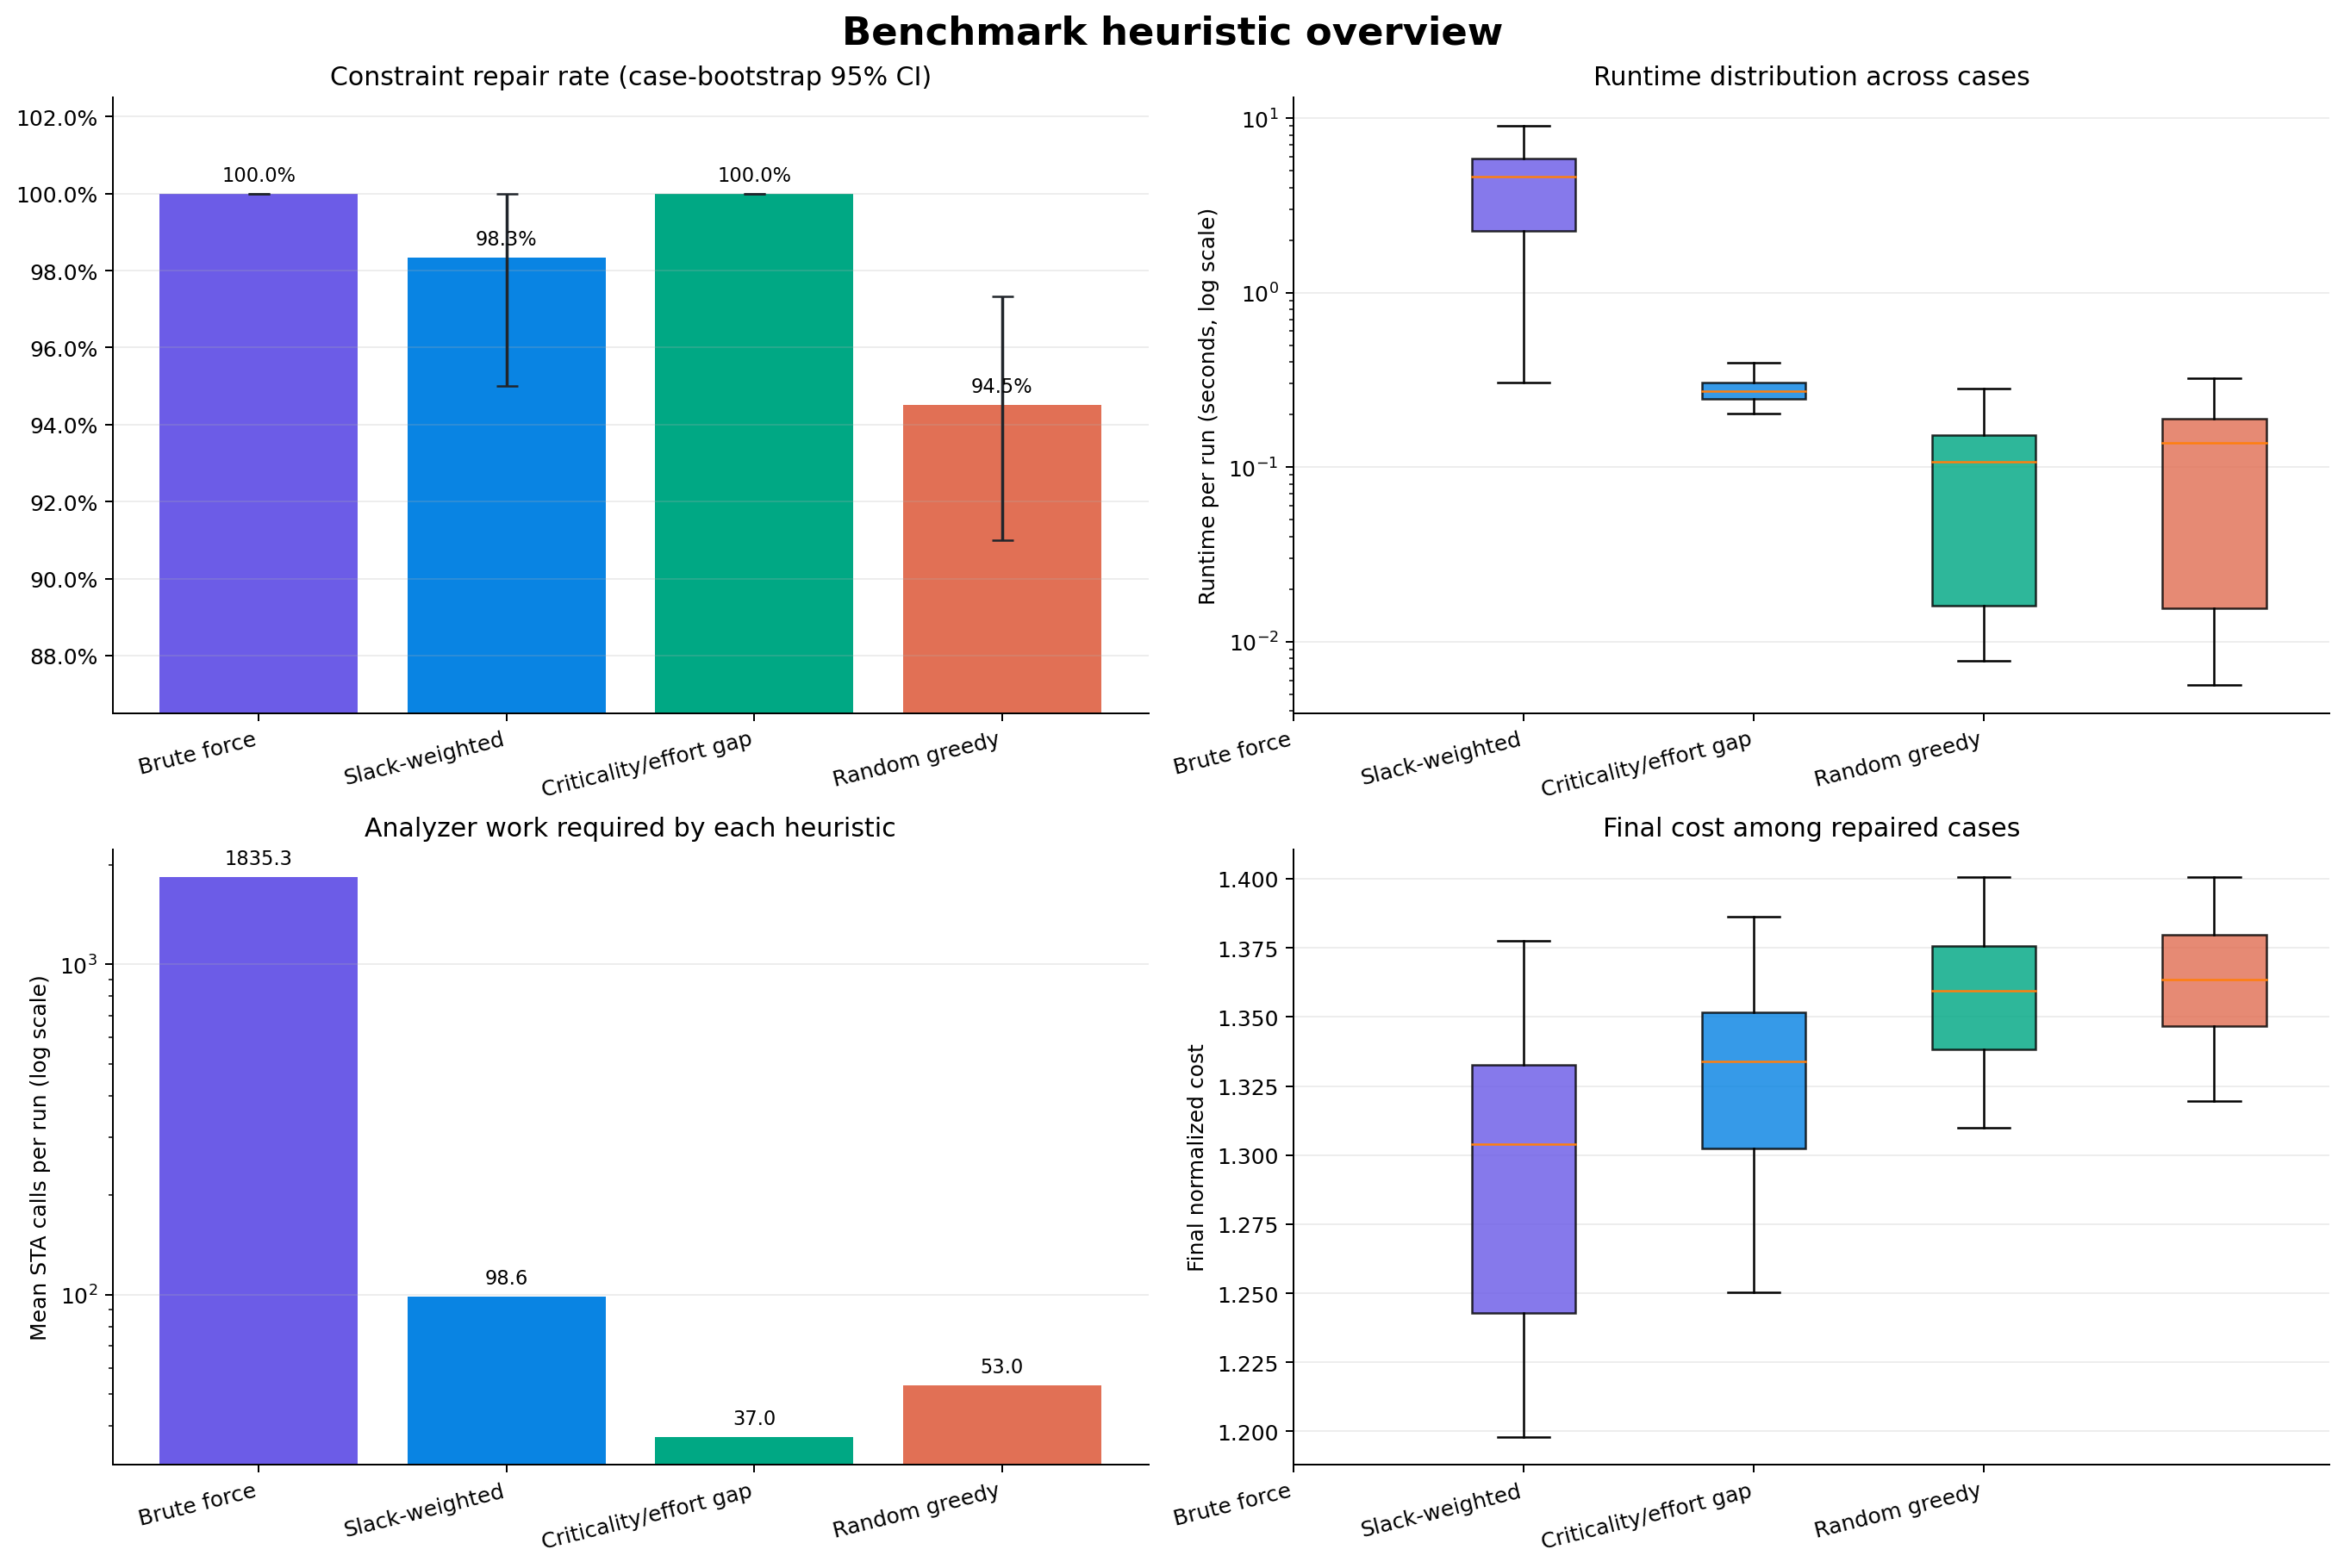
\includegraphics[width=0.7\textwidth]{benchmarking/heuristic_overview}
%     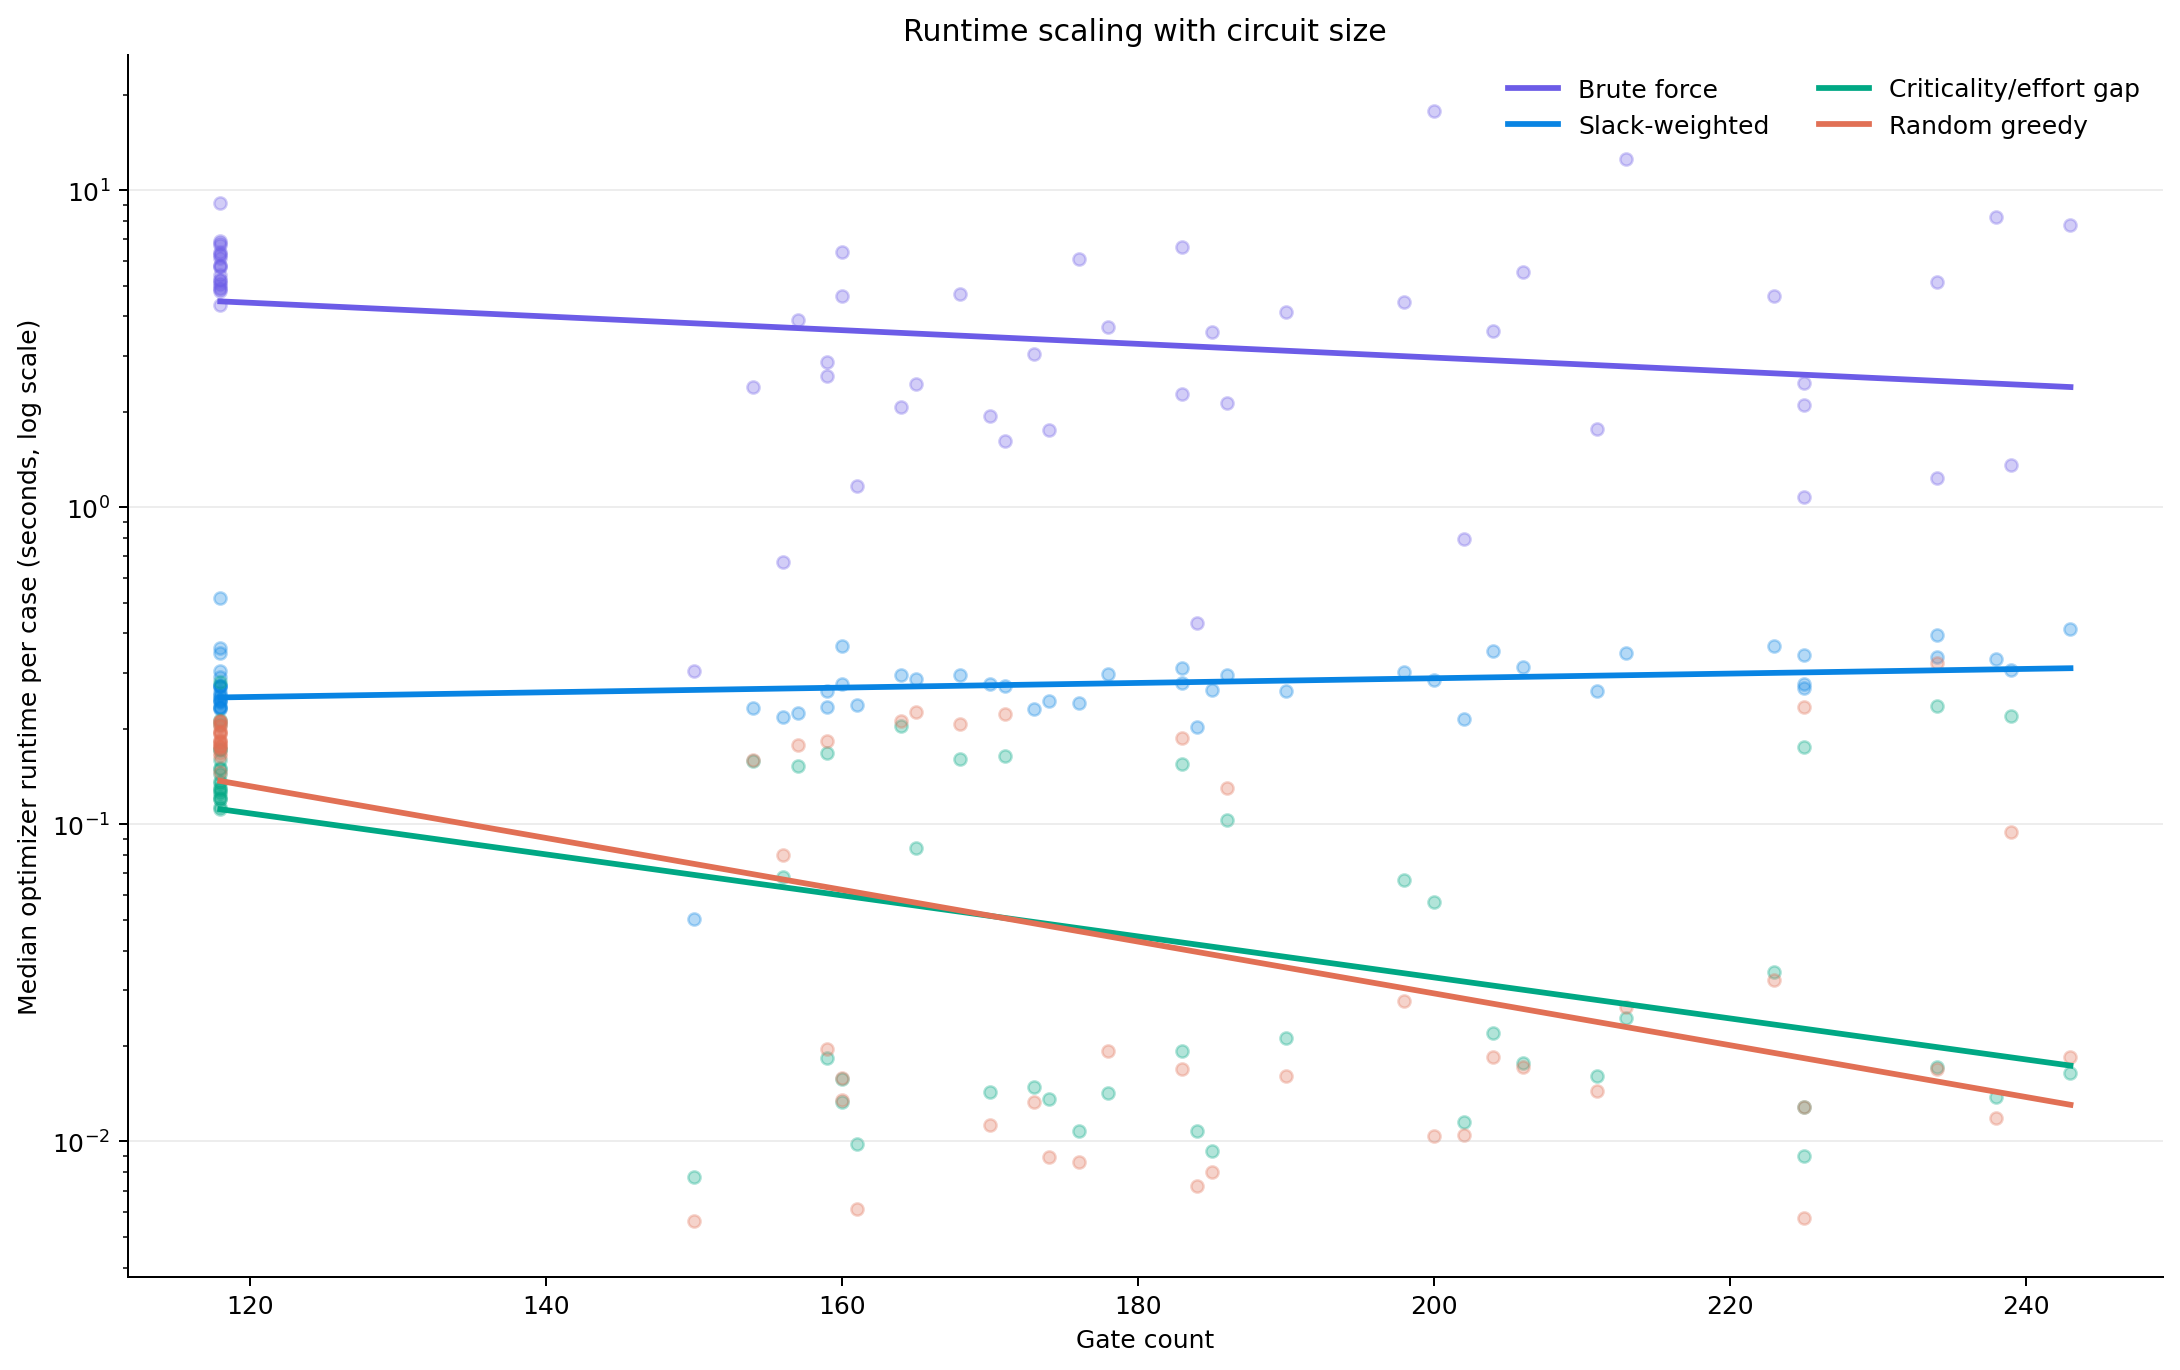
\includegraphics[width=0.7\textwidth]{benchmarking/runtime_scalability}
%     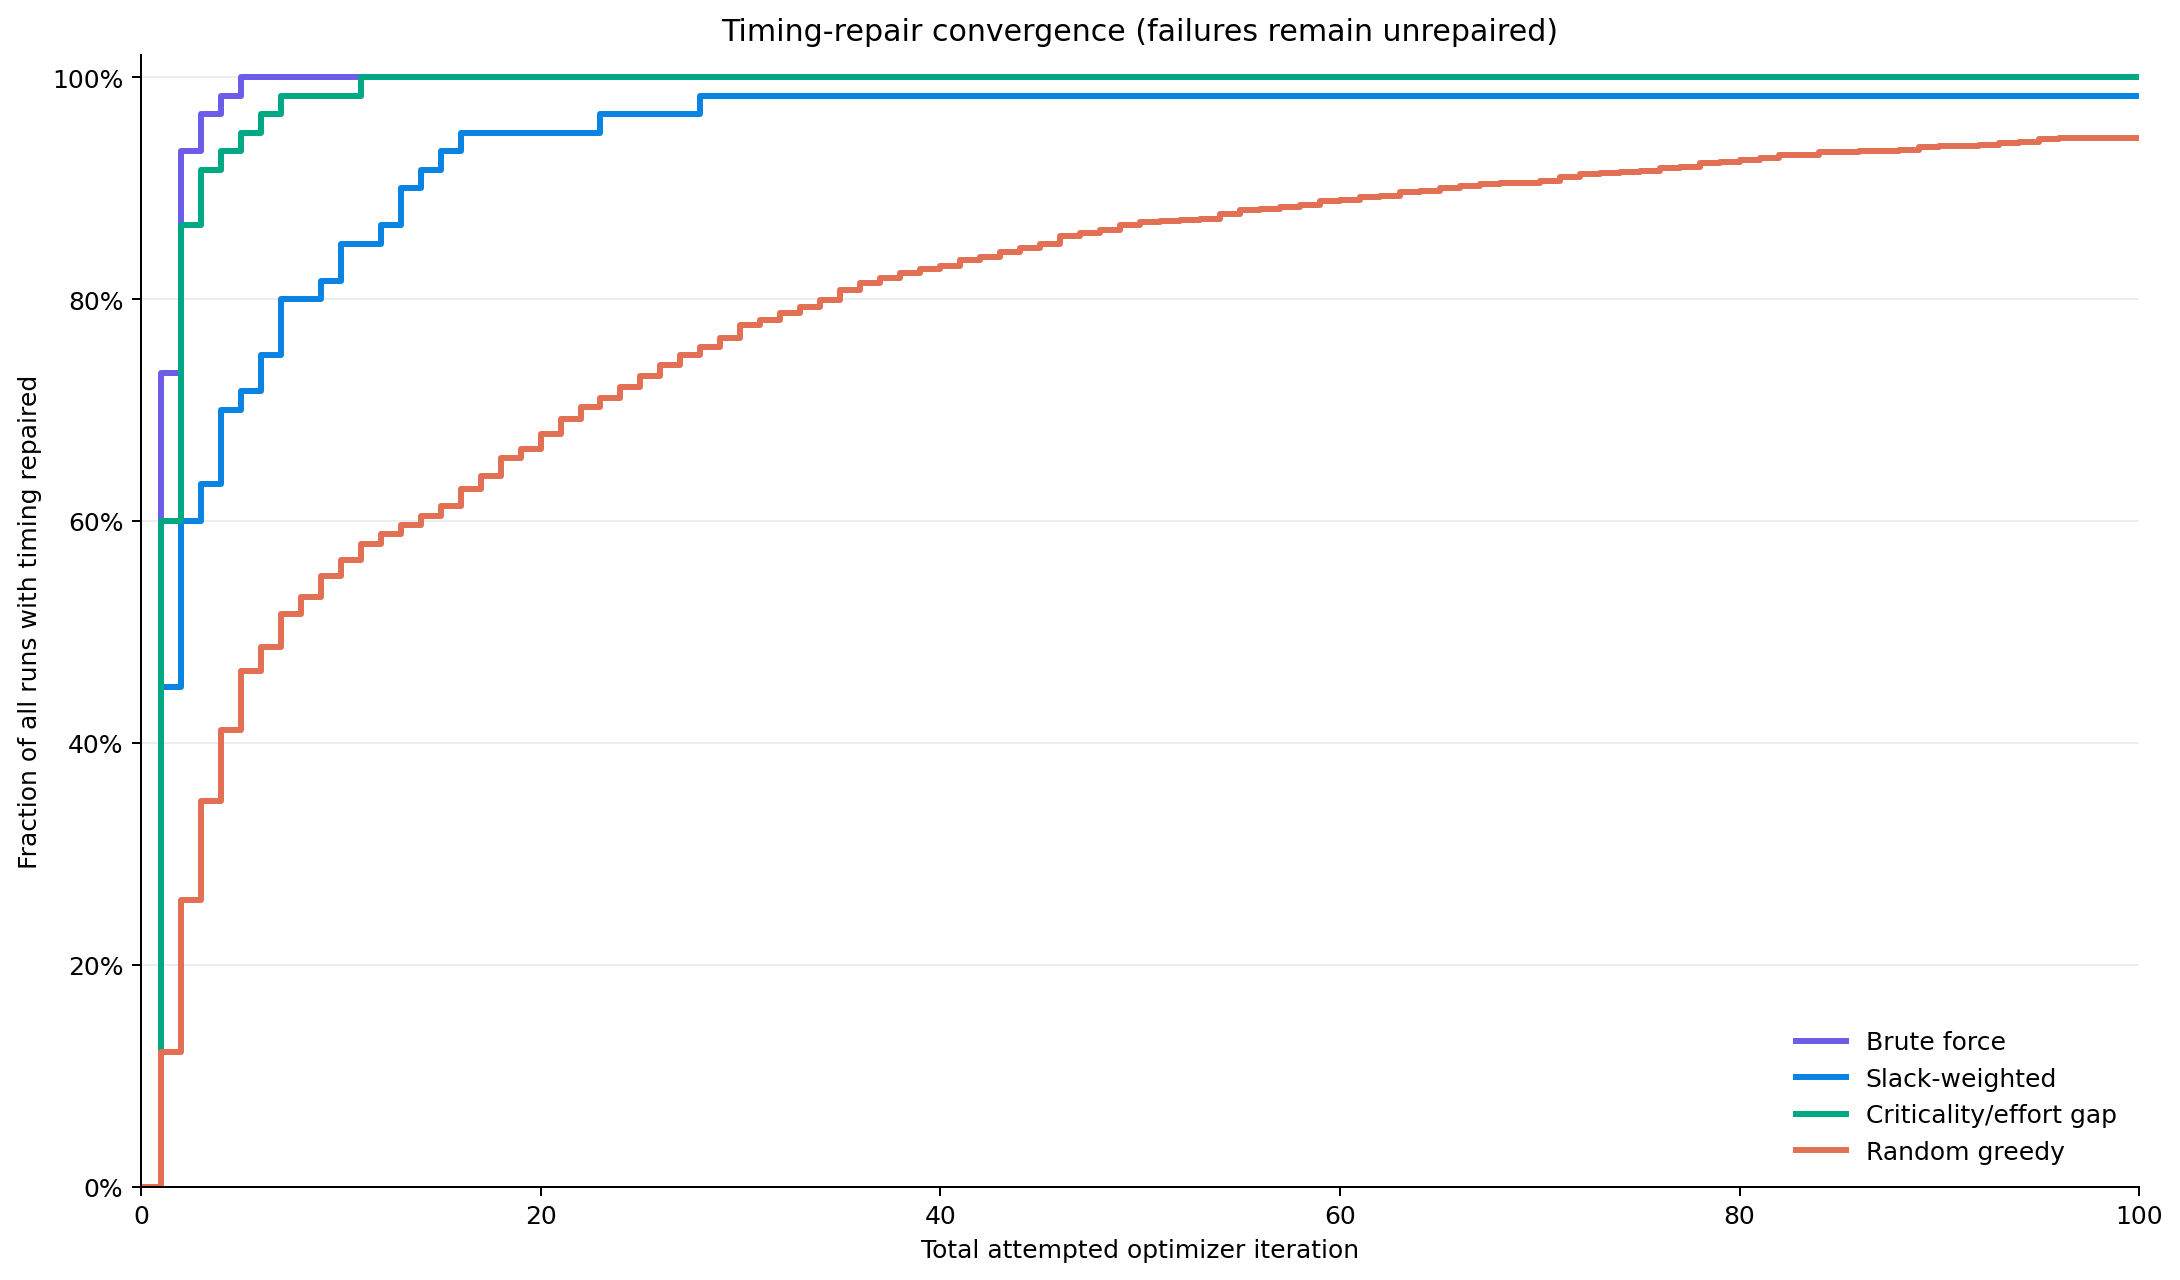
\includegraphics[width=0.7\textwidth]{benchmarking/repair_convergence}
%     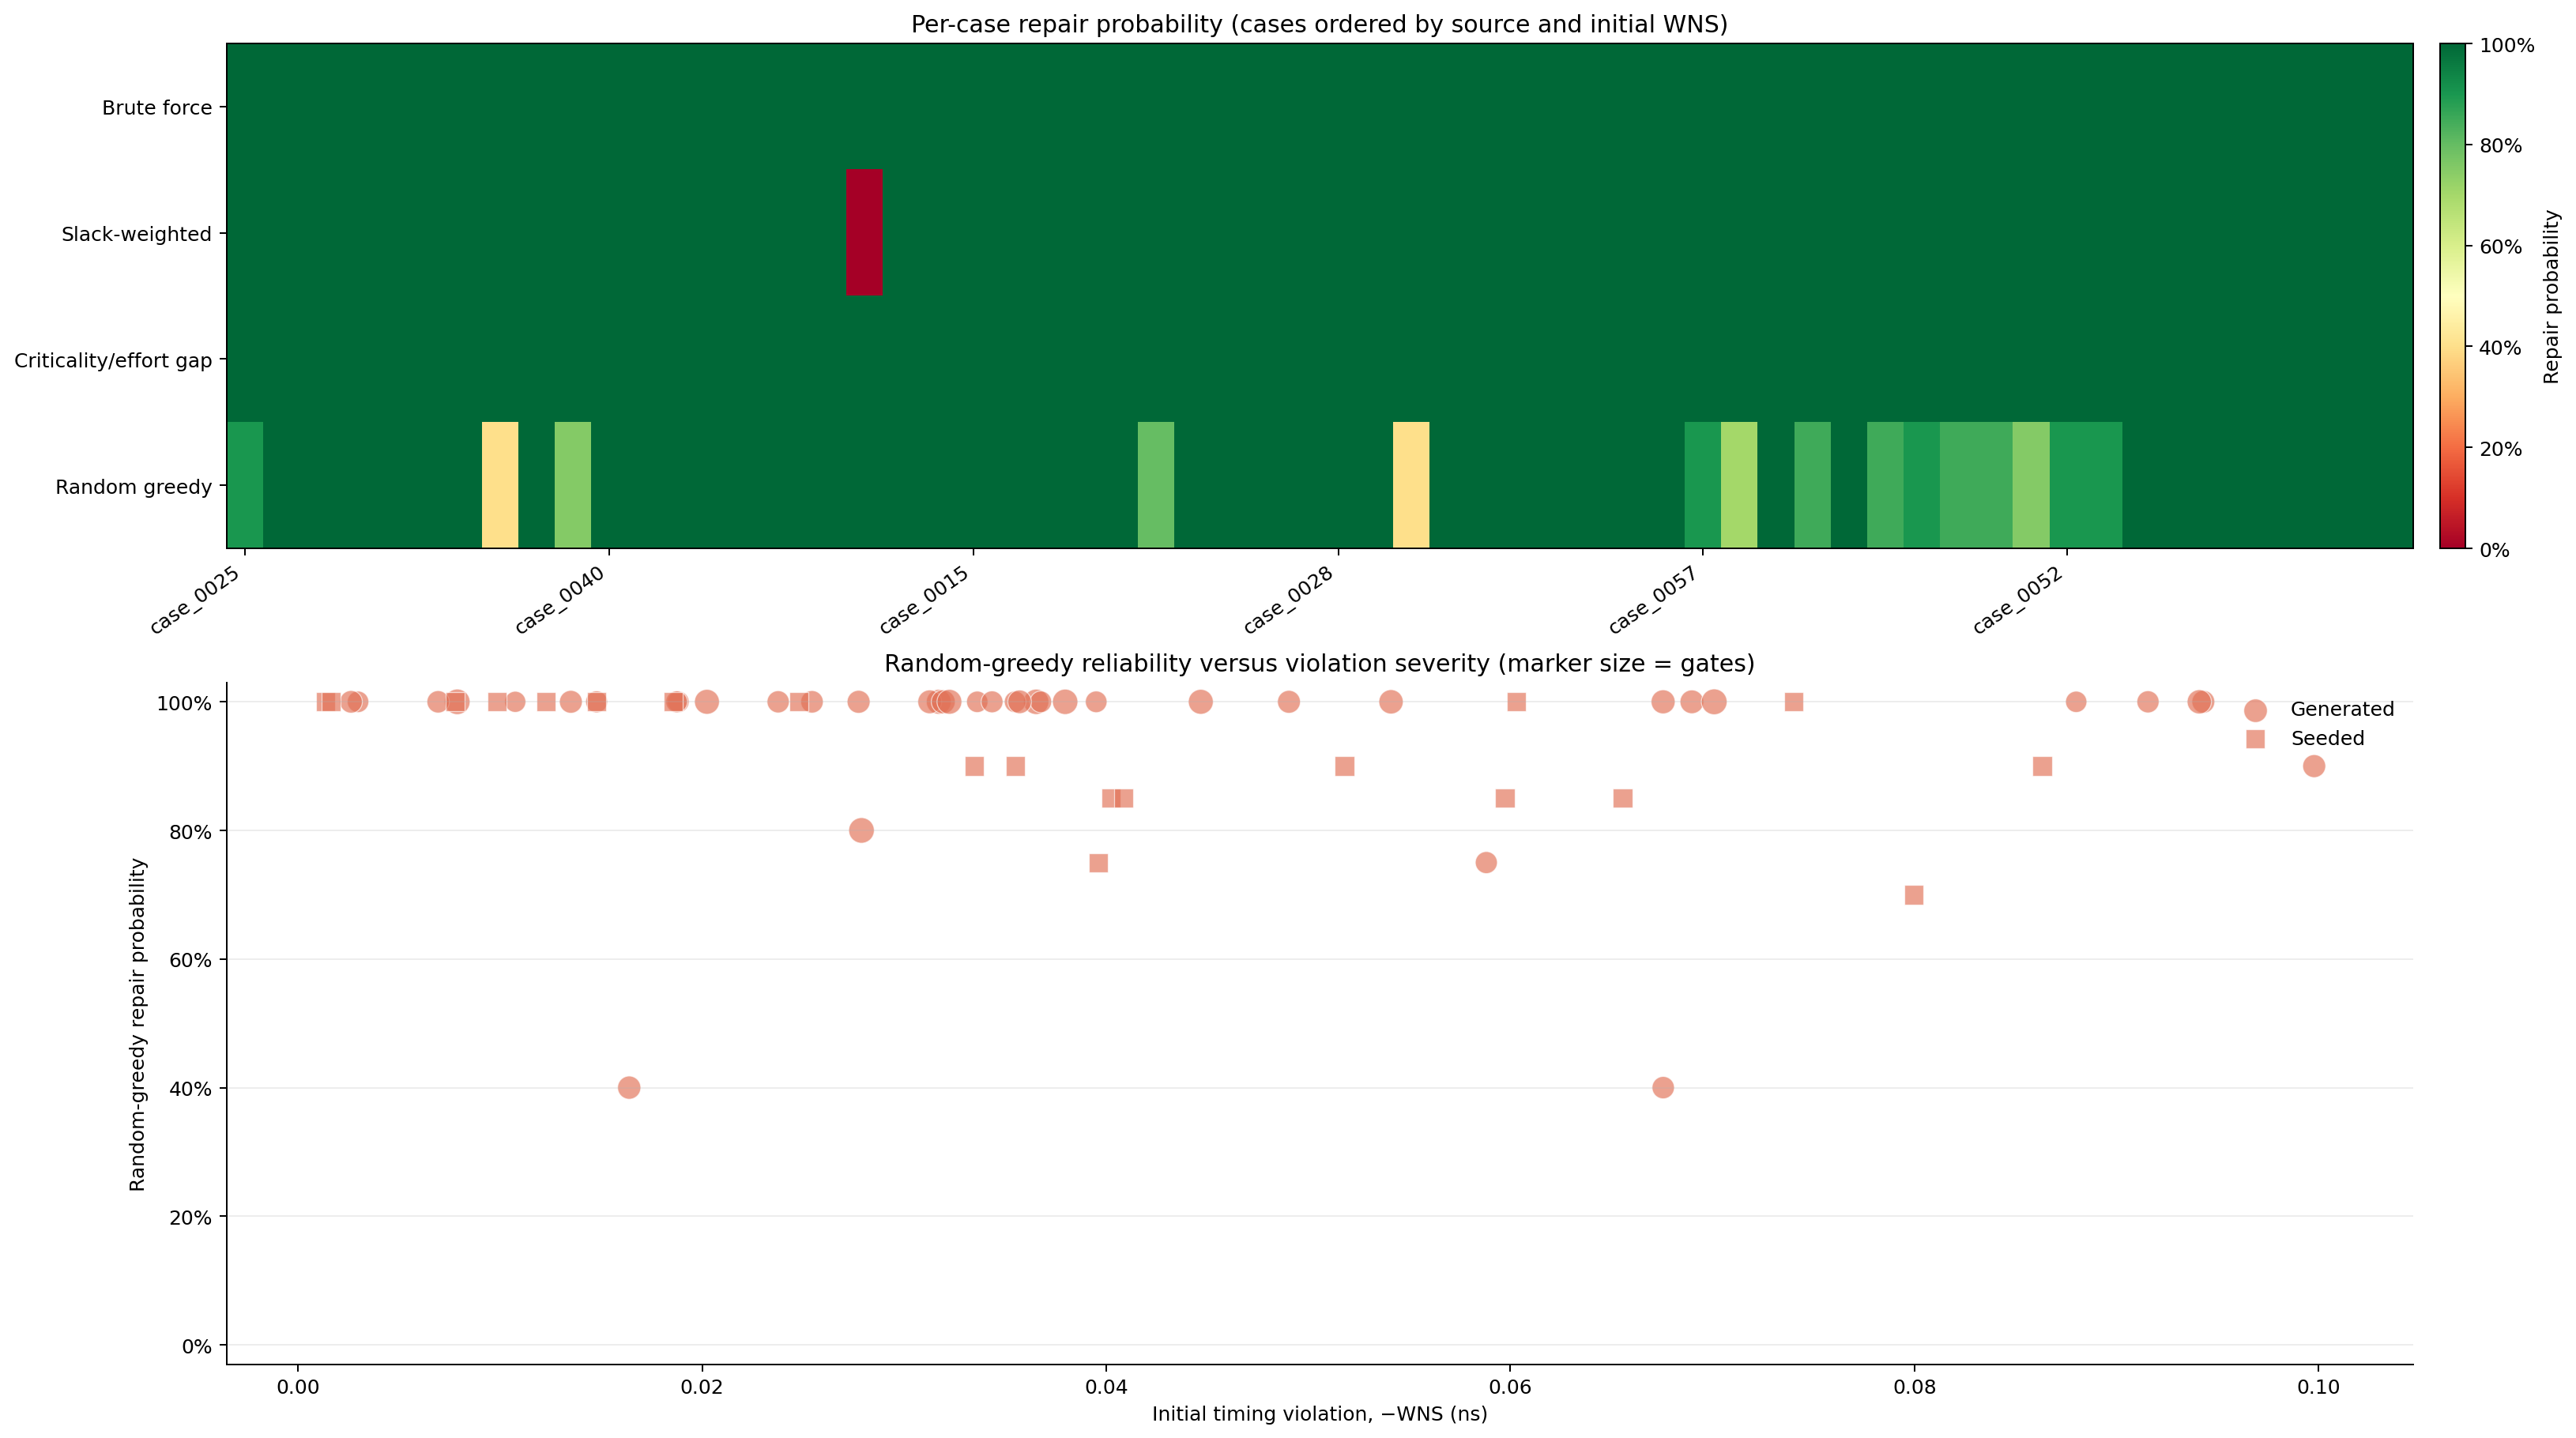
\includegraphics[width=0.7\textwidth]{benchmarking/case_reliability}
%     \caption{Example output of the benchmark plotting command. Replace
%     with an actual generated plot from a completed evaluation run.}
%     \label{fig:bench-plot-placeholder}
% \end{figure}

\chapter{Interactive Topology Viewer}
\label{ch:viewer}

\section{Purpose and Architecture}
\label{sec:viewer-purpose}

Static PNG renderings of a circuit's DAG (\code{circuit\_graph\_\{pre,post\}\_optimization.png} artifacts of
\cref{tab:output-contract}) are adequate for small circuits but become
difficult to read once a circuit reaches the size of the larger benchmark
circuits (upwards of a hundred gates) or once a reader wants to compare the
pre- and post-optimization state of the same circuit interactively rather
than by flipping between two static images. The interactive viewer
addresses this: every analysis run exports \code{circuit\_topology.json}, a
versioned, self-contained graph description --- one shared topology
(primary inputs, gates, primary outputs, and named nets) with two named
overlays, \code{original} and \code{canonical\_optimized}, each supplying
per-gate cell assignment, load capacitance, rise/fall delay, and ranked
critical paths for that state of the circuit. A small local server,
launched with

\begin{lstlisting}[language=bash, style=pythonstyle, numbers=none]
vlsi-sta view outputs/c15_high_fanout_sizing_fabric
\end{lstlisting}

serves this JSON contract to a browser-based front end and opens it
automatically (suppressible with \code{--no-browser} for remote or scripted
use, with \code{--host}/\code{--port} available for remote access).

\section{Features}
\label{sec:viewer-features}

\begin{itemize}
    \item Mouse- and touch-based panning, cursor-anchored wheel zoom, and a
          fit-to-view command, with keyboard shortcuts (\code{+}, \code{-},
          \code{F}, \code{0}, \code{Escape}) mirroring the on-screen
          controls.
    \item Optional net labels and node selection, with connected-net
          isolation to declutter the view of a densely fanned-out node.
    \item Independent visibility toggles for the \code{original} and
          \code{canonical\_optimized} overlays, so the two states can be
          viewed separately or superimposed.
    \item Critical-path coloring consistent with the static PNG renderings.
    \item \textbf{Dual-state gate inspection}: selecting a gate shows its
          cell, load, and delay in both the original and optimized state
          side by side.
    \item \textbf{Target-size highlighting} for any gate the optimizer
          resized: an amber halo marks a gate resized to an \code{X2}
          target, a wider purple halo marks a gate resized to an \code{X4}
          target. This highlighting is shown only while both overlays are
          simultaneously enabled, since it is inherently a comparison
          between the two states.
      \item \textbf{Analysis and Schematic View modes}: Analysis view is the
          normal mode (similar to the PNG files), but a \emph{Schematic View} feature
          enables the user to see the real circuit elements instead of boxes.
\end{itemize}

\section{Screenshots}
\label{sec:viewer-screenshots}
\vspace{-10pt}
\begin{figure}[H]
    \centering
    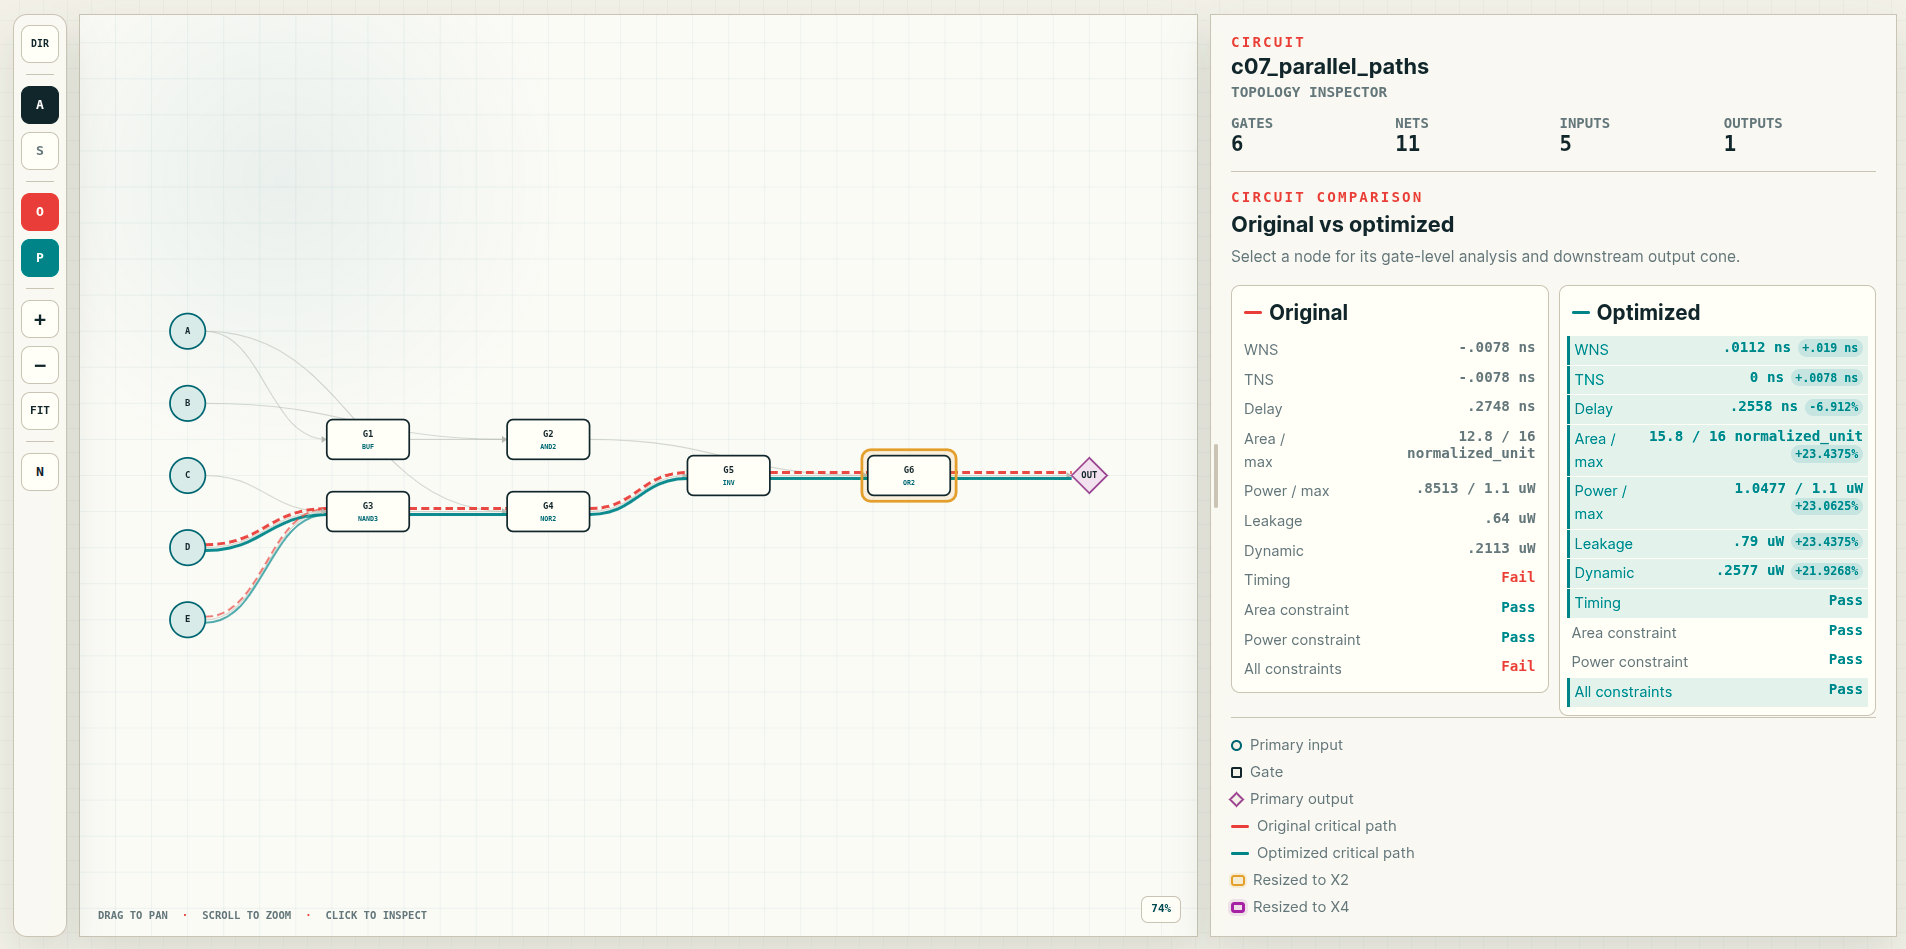
\includegraphics[width=\textwidth]{viewer/analysis view}
    \caption{Interactive topology viewer: Analysis View mode.}
\end{figure}

\begin{figure}[H]
    \centering
    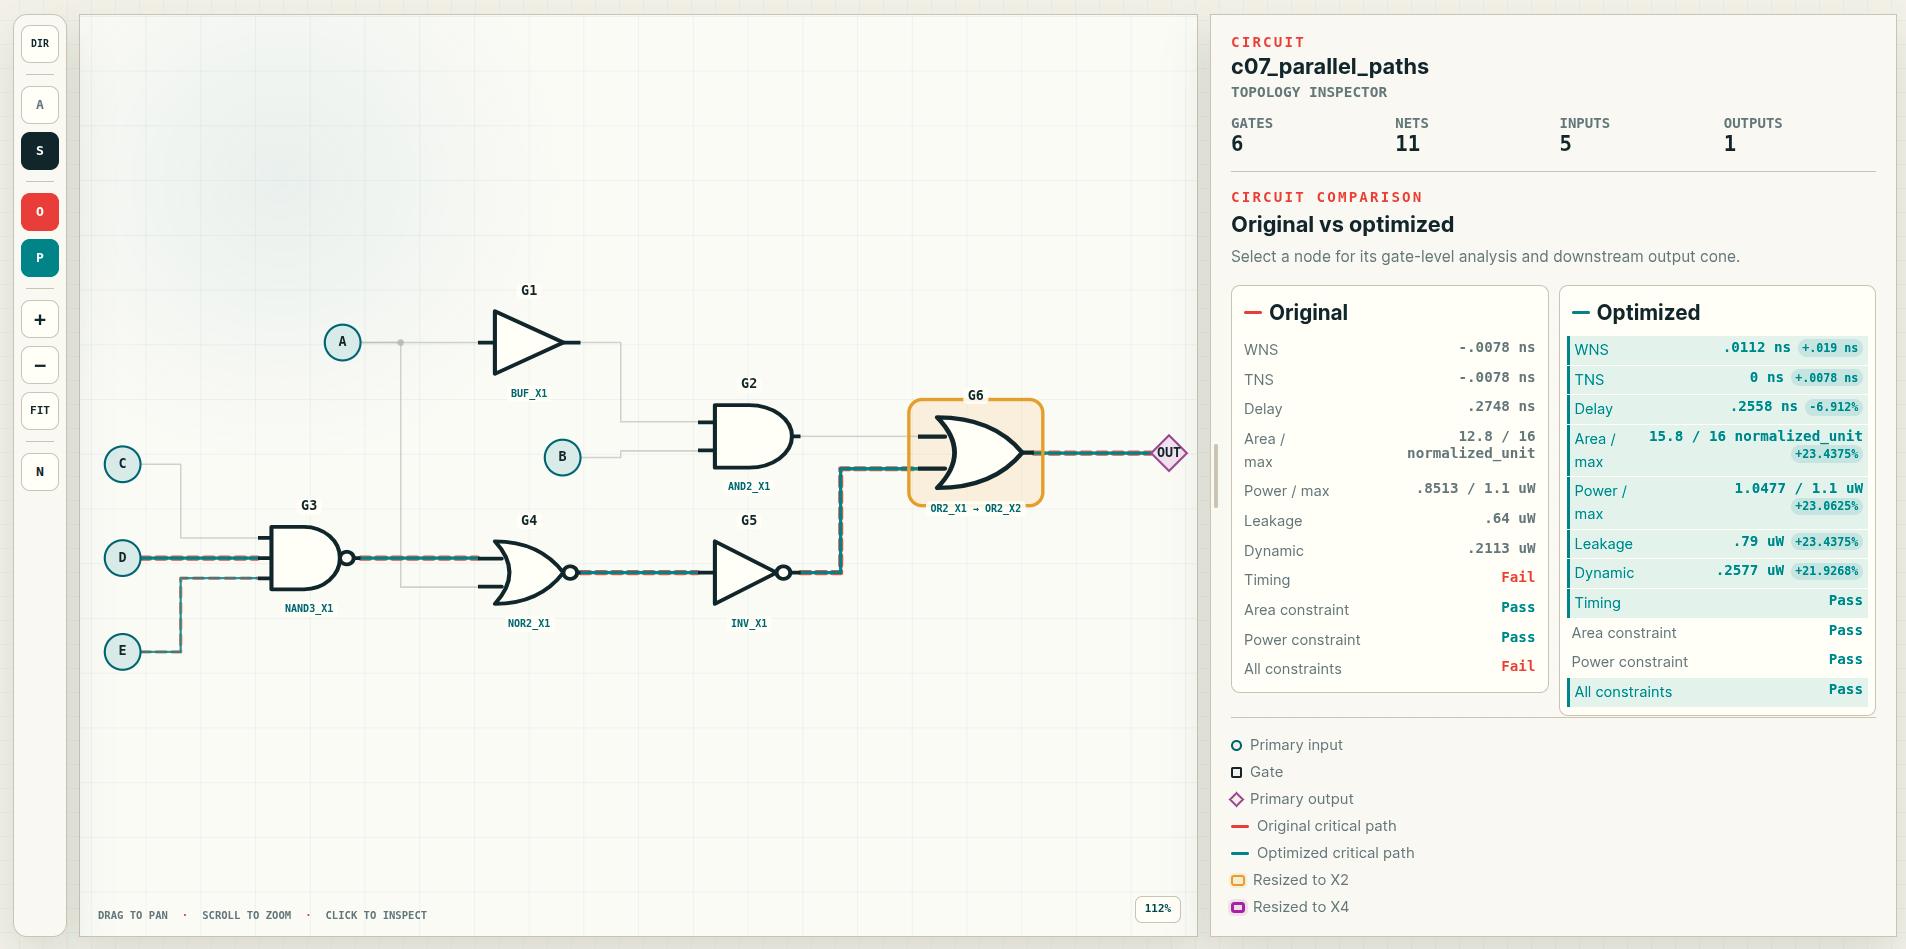
\includegraphics[width=\textwidth]{viewer/schematic view}
    \caption{Interactive topology viewer: Schematic View mode.}
\end{figure}
\vspace{-60pt}

\begin{figure}[H]
    \centering
    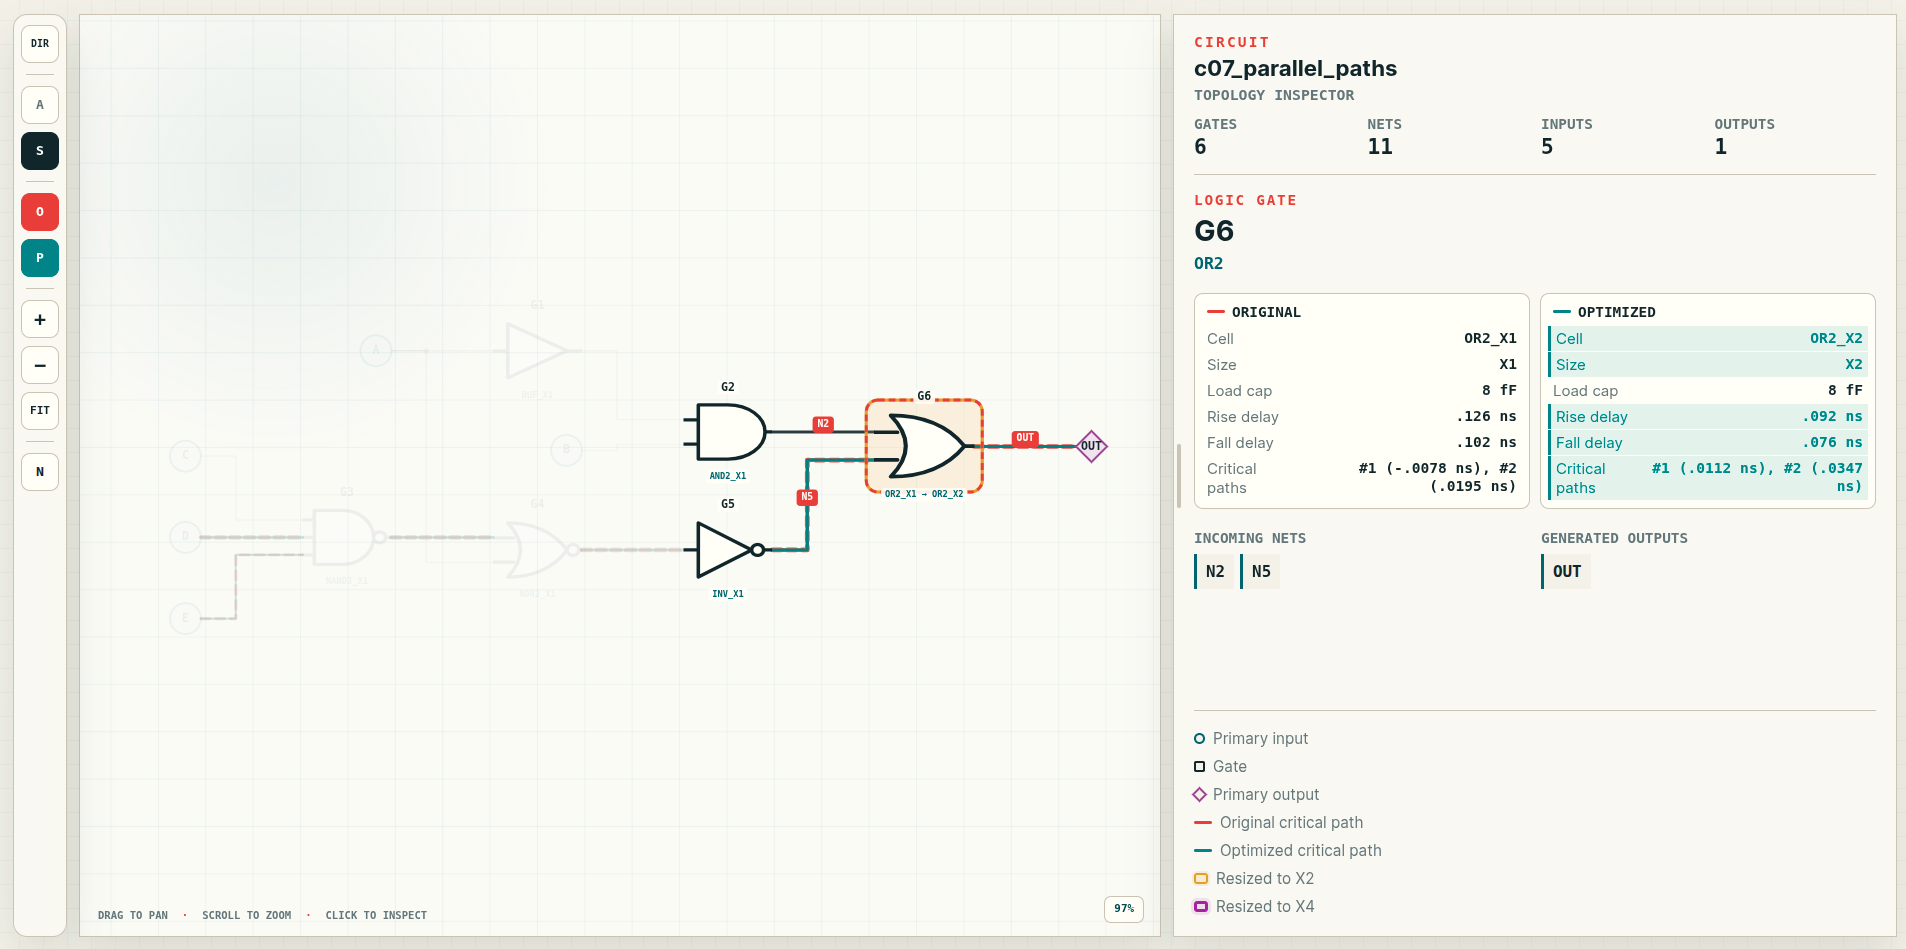
\includegraphics[width=\textwidth]{viewer/gate select}
    \caption{Interactive topology viewer: gate inspection mode (clicked on a gate).}
\end{figure}

\begin{figure}[H]
    \centering
    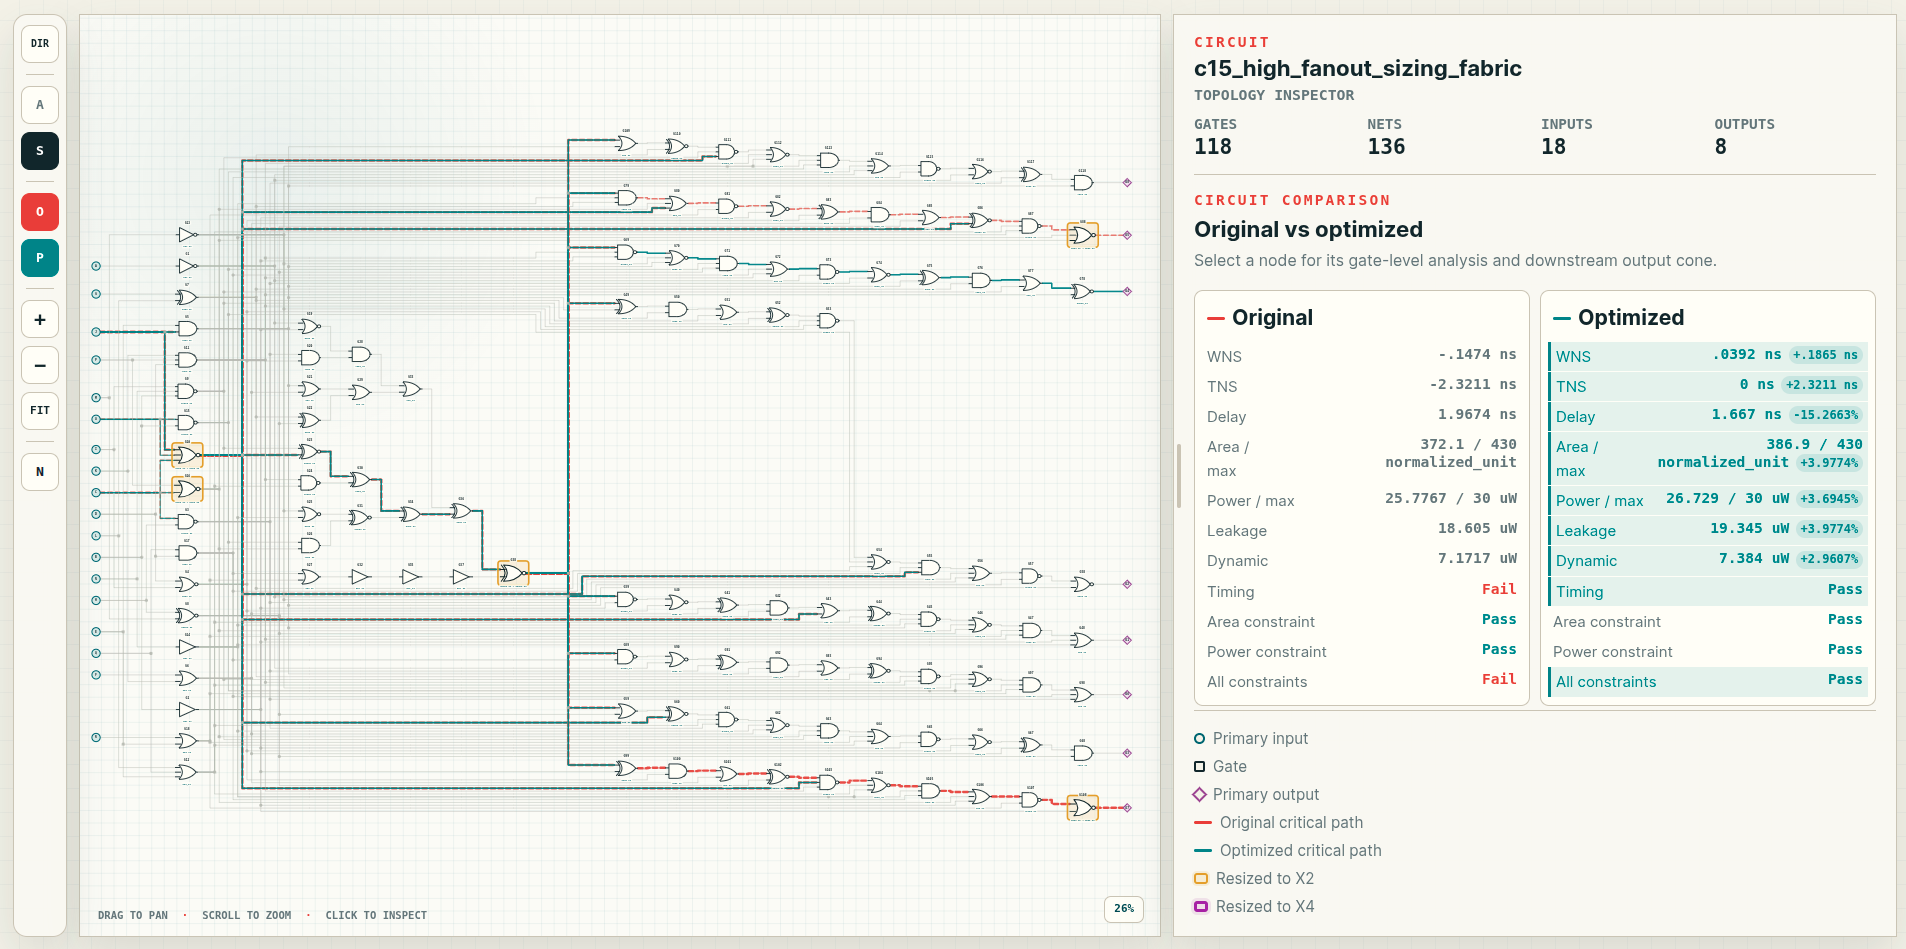
\includegraphics[width=\textwidth]{viewer/big circuit}
    \caption{Interactive topology viewer: Schematic view for a larger circuit.}
\end{figure}

\chapter{Results}
\label{ch:results}

All results in this chapter were produced by running the complete analysis
pipeline (using \code{./run\_circuit.sh --all}) against the fifteen valid and six
invalid benchmark circuits supplied with the assignment, on the codebase
version accompanying this report.

\section{Structural Validation on the Invalid Benchmark Set}
\label{sec:res-invalid}

All six intentionally invalid circuits were correctly rejected, each with
the specific error class the circuit was constructed to exercise
(\cref{tab:error-classes}). \Cref{tab:res-invalid} reproduces the exact
diagnostic message emitted for each.

\begin{table}[H]
\centering
\small
\begin{tabular}{@{}lp{0.62\textwidth}@{}}
\toprule
\textbf{Circuit} & \textbf{Reported diagnostic} \\
\midrule
\code{e01\_undefined\_cell} & \code{undefined cell 'MUX2\_X1'} \\
\code{e02\_undriven\_signal} & \code{signal 'X' is undriven} \\
\code{e03\_multiple\_drivers} & \code{net 'N1' has multiple drivers ('G1' and 'G2')} \\
\code{e04\_combinational\_loop} & \code{combinational loop involving gates: G1, G2, G3} \\
\code{e05\_wrong\_input\_count} & \code{cell 'NAND2\_X1' expects 2 inputs, got 1} \\
\code{e06\_undriven\_output} & \code{primary output 'OUT' is undriven} \\
\bottomrule
\end{tabular}
\caption{Validation results on the six invalid benchmark circuits.}
\label{tab:res-invalid}
\end{table}

\section{Nominal Timing on the Valid Benchmark Set}
\label{sec:res-nominal}

\Cref{tab:res-nominal} reports, for all fifteen valid circuits, the gate
count and the nominal (pre-optimization) circuit delay, WNS, and TNS. One of the fifteen circuits (\code{c01\_inverter\_chain}) is already timing-compliant
(nonnegative WNS); the remaining six exhibit a deliberate timing violation
by construction, ranging from a marginal \SI{-0.002}{ns} on
\code{c12\_monte\_carlo\_swit\newline ching} to a severe \SI{-0.147}{ns} (with a TNS
of \SI{-2.321}{ns}, reflecting many simultaneously violating output
transitions) on \code{c15\_high\_fanout\_sizing\_fabric}, the largest
circuit in the suite at 118 gates.

\newpage
\begin{longtable}{@{}lrrrr@{}}
\toprule
\textbf{Circuit} & \textbf{Gates} & \textbf{Delay (ns)} & \textbf{WNS (ns)} & \textbf{TNS (ns)} \\
\midrule
\endhead
c01\_inverter\_chain            & 3   & 0.1010 & \phantom{-}0.0090 & \phantom{-}0.0000 \\
c02\_basic\_nand\_path          & 3   & 0.1620 & -0.0070 & -0.0070 \\
c03\_fanout\_branch             & 4   & 0.2010 & -0.0060 & -0.0060 \\
c04\_reconvergent\_paths        & 5   & 0.2722 & -0.0072 & -0.0072 \\
c05\_multi\_output              & 5   & 0.2253 & -0.0053 & -0.0078 \\
c06\_deep\_critical\_path       & 10  & 0.4527 & -0.0227 & -0.0268 \\
c07\_parallel\_paths            & 6   & 0.2748 & -0.0078 & -0.0078 \\
c08\_non\_unate\_logic          & 4   & 0.2687 & -0.0087 & -0.0130 \\
c09\_high\_fanout               & 6   & 0.2090 & -0.0040 & -0.0073 \\
c10\_three\_input\_gates        & 5   & 0.2870 & -0.0120 & -0.0120 \\
c11\_gate\_sizing\_stress       & 6   & 0.3595 & -0.0295 & -0.0295 \\
c12\_monte\_carlo\_switching    & 7   & 0.3172 & -0.0022 & -0.0022 \\
c13\_large\_reconvergent\_network & 74  & 1.0103 & -0.0293 & -0.2133 \\
c14\_layered\_reconvergent\_fabric & 104 & 0.9893 & -0.0213 & -0.1596 \\
c15\_high\_fanout\_sizing\_fabric & 118 & 1.9674 & -0.1474 & -2.3211 \\
\bottomrule
\caption{Nominal (pre-optimization) timing on the fifteen valid benchmark
circuits. Nine of fifteen circuits are supplied already timing-compliant;
the remaining six exhibit a constructed violation.}
\label{tab:res-nominal}
\end{longtable}

\section{Gate-Sizing Heuristic Comparison}
\label{sec:res-heuristics}

\Cref{tab:res-heuristics} reports the final WNS reached by each of the
three automatically-invoked heuristics (\code{slack\_weighted\_capacitance},
the canonical logical-effort-guided method; \code{critical\newline ity\_effort\_gap},
the second logical-effort-informed heuristic; and \code{random\_greedy}, the
non-logical-effort baseline), together with a compliance flag indicating
whether that heuristic reached a fully timing-compliant final design within
the configured area and power budgets.

\begin{center}
    

\begin{longtable}{@{}lrrr@{}}
\toprule
\textbf{Circuit} & \textbf{WNS$_{\mathrm{swg}}$} & \textbf{WNS$_{\mathrm{ceg}}$} & \textbf{WNS$_{\mathrm{rg}}$} \\
\midrule
\endhead
c01\_inverter\_chain            & \phantom{-}0.0090 & \phantom{-}0.0090 & \phantom{-}0.0090 \\
c02\_basic\_nand\_path          & \phantom{-}0.0050 & \phantom{-}0.0050 & -0.0010  \\
c03\_fanout\_branch             & \phantom{-}0.0150 & \phantom{-}0.0150 & \phantom{-}0.0150 \\
c04\_reconvergent\_paths        & \phantom{-}0.0059 & \phantom{-}0.0059 & \phantom{-}0.0069 \\
c05\_multi\_output              & -0.0025 & -0.0025 & -0.0053 \\
c06\_deep\_critical\_path       & \phantom{-}0.0033 & \phantom{-}0.0033 & -0.0217 \\
c07\_parallel\_paths            & \phantom{-}0.0112 & \phantom{-}0.0112 & -0.0078 \\
c08\_non\_unate\_logic          & \phantom{-}0.0093 & \phantom{-}0.0093 & \phantom{-}0.0093 \\
c09\_high\_fanout               & \phantom{-}0.0430 & \phantom{-}0.0430 & \phantom{-}0.0430 \\
c10\_three\_input\_gates        & \phantom{-}0.0330 & \phantom{-}0.0330 & \phantom{-}0.0330 \\
c11\_gate\_sizing\_stress       & \phantom{-}0.0325 & \phantom{-}0.0325 & -0.0220 \\
c12\_monte\_carlo\_switching    & \phantom{-}0.0129 & \phantom{-}0.0129 & -0.0002 \\
c13\_large\_reconvergent\_network & \phantom{-}0.0037 & -0.0293 & -0.0293 \\
c14\_layered\_reconvergent\_fabric & \phantom{-}0.0182 & \phantom{-}0.0182 & \phantom{-}0.0030 \\
c15\_high\_fanout\_sizing\_fabric & \phantom{-}0.0392 & \phantom{-}0.0397 & \phantom{-}0.0397 \\
\midrule
\textbf{Repair rate} & \textbf{14/15} & \textbf{13/15} & \textbf{8/15} \\
\bottomrule
\caption{Final WNS (ns) and compliance status per heuristic. Repair rate
counts circuits reaching \(\mathrm{WNS} \geq 0\) within area/power
budgets, out of all fifteen valid circuits.}
\label{tab:res-heuristics}
\end{longtable}
\end{center}

Restricted to only the fourteen circuits that exhibited a violation to
begin with (excluding \code{c01}, already compliant), the repair rates are
$13/14$ ($\approx 92.9\%$) for slack-weighted capacitance, $12/14$
($\approx 85.7\%$) for criticality effort gap, and $7/14$ ($=50.0\%$) for
random greedy heuristic.

\subsection{Efficiency: STA Calls}
\label{sec:res-efficiency}

Summed across all fifteen circuits, the canonical logical-effort-guided
heuristic issued \textbf{119} total STA calls, versus \textbf{155} for
random greedy --- and the correct explanation for this is more specific
than ``one attempt, one STA call.'' \Cref{sec:opt-eval} already
establishes that candidate evaluation is a two-step gate: a cheap,
STA-free pre-filter (\code{replacement\_area\_and\_po\newline wer}) rejects a
candidate outright if it alone would exceed the area or power budget,
and only a candidate that survives this filter reaches the actual
\code{analyze\_timing} call. Cross-checking the recorded iteration logs
confirms this directly: on \code{c13\_large\_reconvergent\_network}, the
canonical heuristic's log contains 66 logged attempts, of which 52 are
rejected with reason \emph{``candidate violates area or power
constraints''} (free, no STA call) and only 13 require an actual timing
result (10 rejected for not improving WNS/TNS, 1 rejected once compliant
for not improving cost, and 2 accepted) --- plus one further STA call to
establish the initial reference state (\cref{sec:opt-cost}), for a
reported total of 14, exactly matching \code{summary.json}.

Because budget-infeasible candidates cost nothing, a heuristic's STA-call
total measures how many candidates it proposes that are \emph{plausible
enough to need a real timing check}, not merely how many candidates it
tries in total. On this specific circuit, random greedy needed only 3 STA
calls in total (1 initial, 1 accepted, 1 WNS/TNS rejection) against the
canonical heuristic's 14 --- the canonical heuristic's higher-scored
candidates more often clear the cheap budget pre-filter and therefore more
often reach the expensive check, while most of random greedy's random
draws are eliminated for free before ever costing a timing analysis. This
cautions against reading the suite-wide STA-call total as a simple
``search order wastes fewer attempts'' story: the totals do favor the
canonical heuristic in aggregate (119 versus 155) and as a per-circuit
mean ($\approx 7.9$ versus $\approx 10.3$ calls per circuit), but not
uniformly --- on five of the fifteen circuits, including the two largest
(\code{c13}: 14 versus 3; \code{c14}: 39 versus 19), the canonical
heuristic issues \emph{more} STA calls than random greedy, precisely
because more of its proposals are good enough to be worth the expensive
check in the first place. Aggregate STA-call count is therefore best read
as a rough proxy for total search cost, not as a clean, uniformly-favorable
efficiency metric on its own; \cref{tab:res-heuristics,tab:res-cost}'s
repair-rate and final-cost comparisons are the more direct evidence for
the canonical heuristic's advantage.

\subsection{Cost, Power, and Area}
\label{sec:res-cost}

\Cref{tab:res-cost} compares the final cost $J$ (\cref{eq:cost}) reached by
the canonical heuristic against random greedy. The canonical method
reaches a \emph{strictly} lower (better) final cost than random greedy on
ten of the fifteen circuits, and \emph{ties exactly} on the remaining
five: on \code{c01} because neither heuristic makes any accepted change at
all (the circuit is already compliant and no candidate reduces cost), and
on \code{c03}, \code{c08}, \code{c09}, and \code{c10} because both
heuristics independently accept the identical sequence of resizes (verified
directly against the recorded iteration logs, not merely inferred from
matching final cost). On \emph{no} circuit in the suite does random greedy
reach a lower final cost than the canonical heuristic. The narrowest
margin in the canonical method's favor is on \code{c15}
($J = 1.263$ versus $J = 1.272$), still a real, if small, improvement
rather than a tie.

\begin{longtable}{@{}lrrr@{}}
\toprule
\textbf{Circuit} & \textbf{$J_0$} & \textbf{$J_{\mathrm{swc}}$} & \textbf{$J_{\mathrm{rg}}$} \\
\midrule
\endhead
c01\_inverter\_chain            & 1.400 & 1.400 & 1.400 \\
c02\_basic\_nand\_path          & 1.616 & 1.511 & 1.578 \\
c03\_fanout\_branch             & 1.549 & 1.342 & 1.342 \\
c04\_reconvergent\_paths        & 1.532 & 1.434 & 1.481 \\
c05\_multi\_output              & 1.518 & 1.466 & 1.587 \\
c06\_deep\_critical\_path       & 1.650 & 1.377 & 1.659 \\
c07\_parallel\_paths            & 1.543 & 1.424 & 1.573 \\
c08\_non\_unate\_logic          & 1.561 & 1.376 & 1.376 \\
c09\_high\_fanout               & 1.496 & 1.207 & 1.207 \\
c10\_three\_input\_gates        & 1.609 & 1.368 & 1.368 \\
c11\_gate\_sizing\_stress       & 1.810 & 1.283 & 1.780 \\
c12\_monte\_carlo\_switching    & 1.434 & 1.412 & 1.444 \\
c13\_large\_reconvergent\_network & 1.545 & 1.376 & 1.551 \\
c14\_layered\_reconvergent\_fabric & 1.508 & 1.291 & 1.375 \\
c15\_high\_fanout\_sizing\_fabric & 1.775 & 1.263 & 1.272 \\
\bottomrule
\caption{Final cost function value $J$, initial versus
each heuristic's final design.}
\label{tab:res-cost}
\end{longtable}

\subsection{Case Study: \texttt{c02\_basic\_nand\_path}}
\label{sec:res-case-c02}

\Cref{fig:c02-pre,fig:c02-post} show the rendered pre- and
post-optimization circuit diagrams for the smallest circuit on which
slack-weighted capacitance and random greedy diverge in outcome, and the
full recorded iteration logs
(\code{optimization\_slack\_weighted\_capacitance.csv},
\code{optimization\_random\_greedy.csv}) make the reason for the divergence
precisely traceable rather than merely inferable from the final numbers.

Slack-weighted capacitance's very first candidate --- ranked highest by
its urgency$\times$mismatch score (\cref{sec:opt-swc}) --- is
\code{G3: AND2\_X1}$\rightarrow$\code{AND2\_X2}, which alone resolves the
violation ($\mathrm{WNS}: -0.0070 \rightarrow +0.0050$~ns) in one accepted
change. Three further candidates (\code{G1}, \code{G3}$\rightarrow$
\code{X4}, \code{G2}) are then proposed by the cost-reduction phase
(\cref{sec:opt-accept}) and all three are \emph{rejected} for violating the
configured area/power budget, at which point the search terminates
\code{no\_feasible\_change} --- a normal, compliant stop, not a failure.

Random greedy's uniformly random draw instead tries \code{G1:
NAND2\_X1}$\rightarrow$\code{X2} first (accepted; $\mathrm{WNS}:
-0.0070\rightarrow-0.0025$~ns, an improvement but not yet compliant), then
rejects \code{G3: AND2\_X1}$\rightarrow$\code{X2} for exceeding the area
budget (at this point, with \code{G1} already upsized, the combined area
would reach $10.2$, well past the $8.5$ limit), then accepts \code{G2:
INV\_X1}$\rightarrow$\code{X2} (WNS$\rightarrow-0.0010$~ns), and finally
exhausts its remaining candidates (\code{G1}$\rightarrow$\code{X4},
\code{G2}$\rightarrow$\code{X4}, a repeated \code{G3}$\rightarrow$\code{X2}
attempt) all rejected on the same area ceiling, terminating
\code{no\_feasible\_change} while \textbf{still in violation}.

Both searches plateau at the identical configured budget ceiling
(\code{maximum\_area} $= 8.5$), reached via two different combinations of
accepted resizes: slack-weighted capacitance reaches a total area of
$8.4$ after its single accepted \code{G3} resize alone, while random
greedy reaches the same $8.4$ via its two smaller accepted resizes
(\code{G1} then \code{G2}) combined. From that point, every further
candidate in \emph{either} run --- regardless of which gate it targets ---
is rejected against the same $8.5$ ceiling; the outcome is decided not by
which gate the budget happens to block, but by whether a compliant WNS was
already reached \emph{before} the ceiling was hit. Slack-weighted
capacitance's score-ranked draw tried the one resize that both fixes the
violation and fits the pristine budget on its very first attempt; random
greedy's random draw spent that same budget across two resizes that
together do not fix the violation, before any further candidate could be
tried. This is a concrete, single-circuit illustration of exactly the
aggregate effect quantified in \cref{sec:res-efficiency}: an informed
search order does not expand what a heuristic is allowed to do, only the
likelihood that a fix is found before the shared budget ceiling is
reached by changes that do not resolve the violation.

\begin{figure}[H]
    \centering
    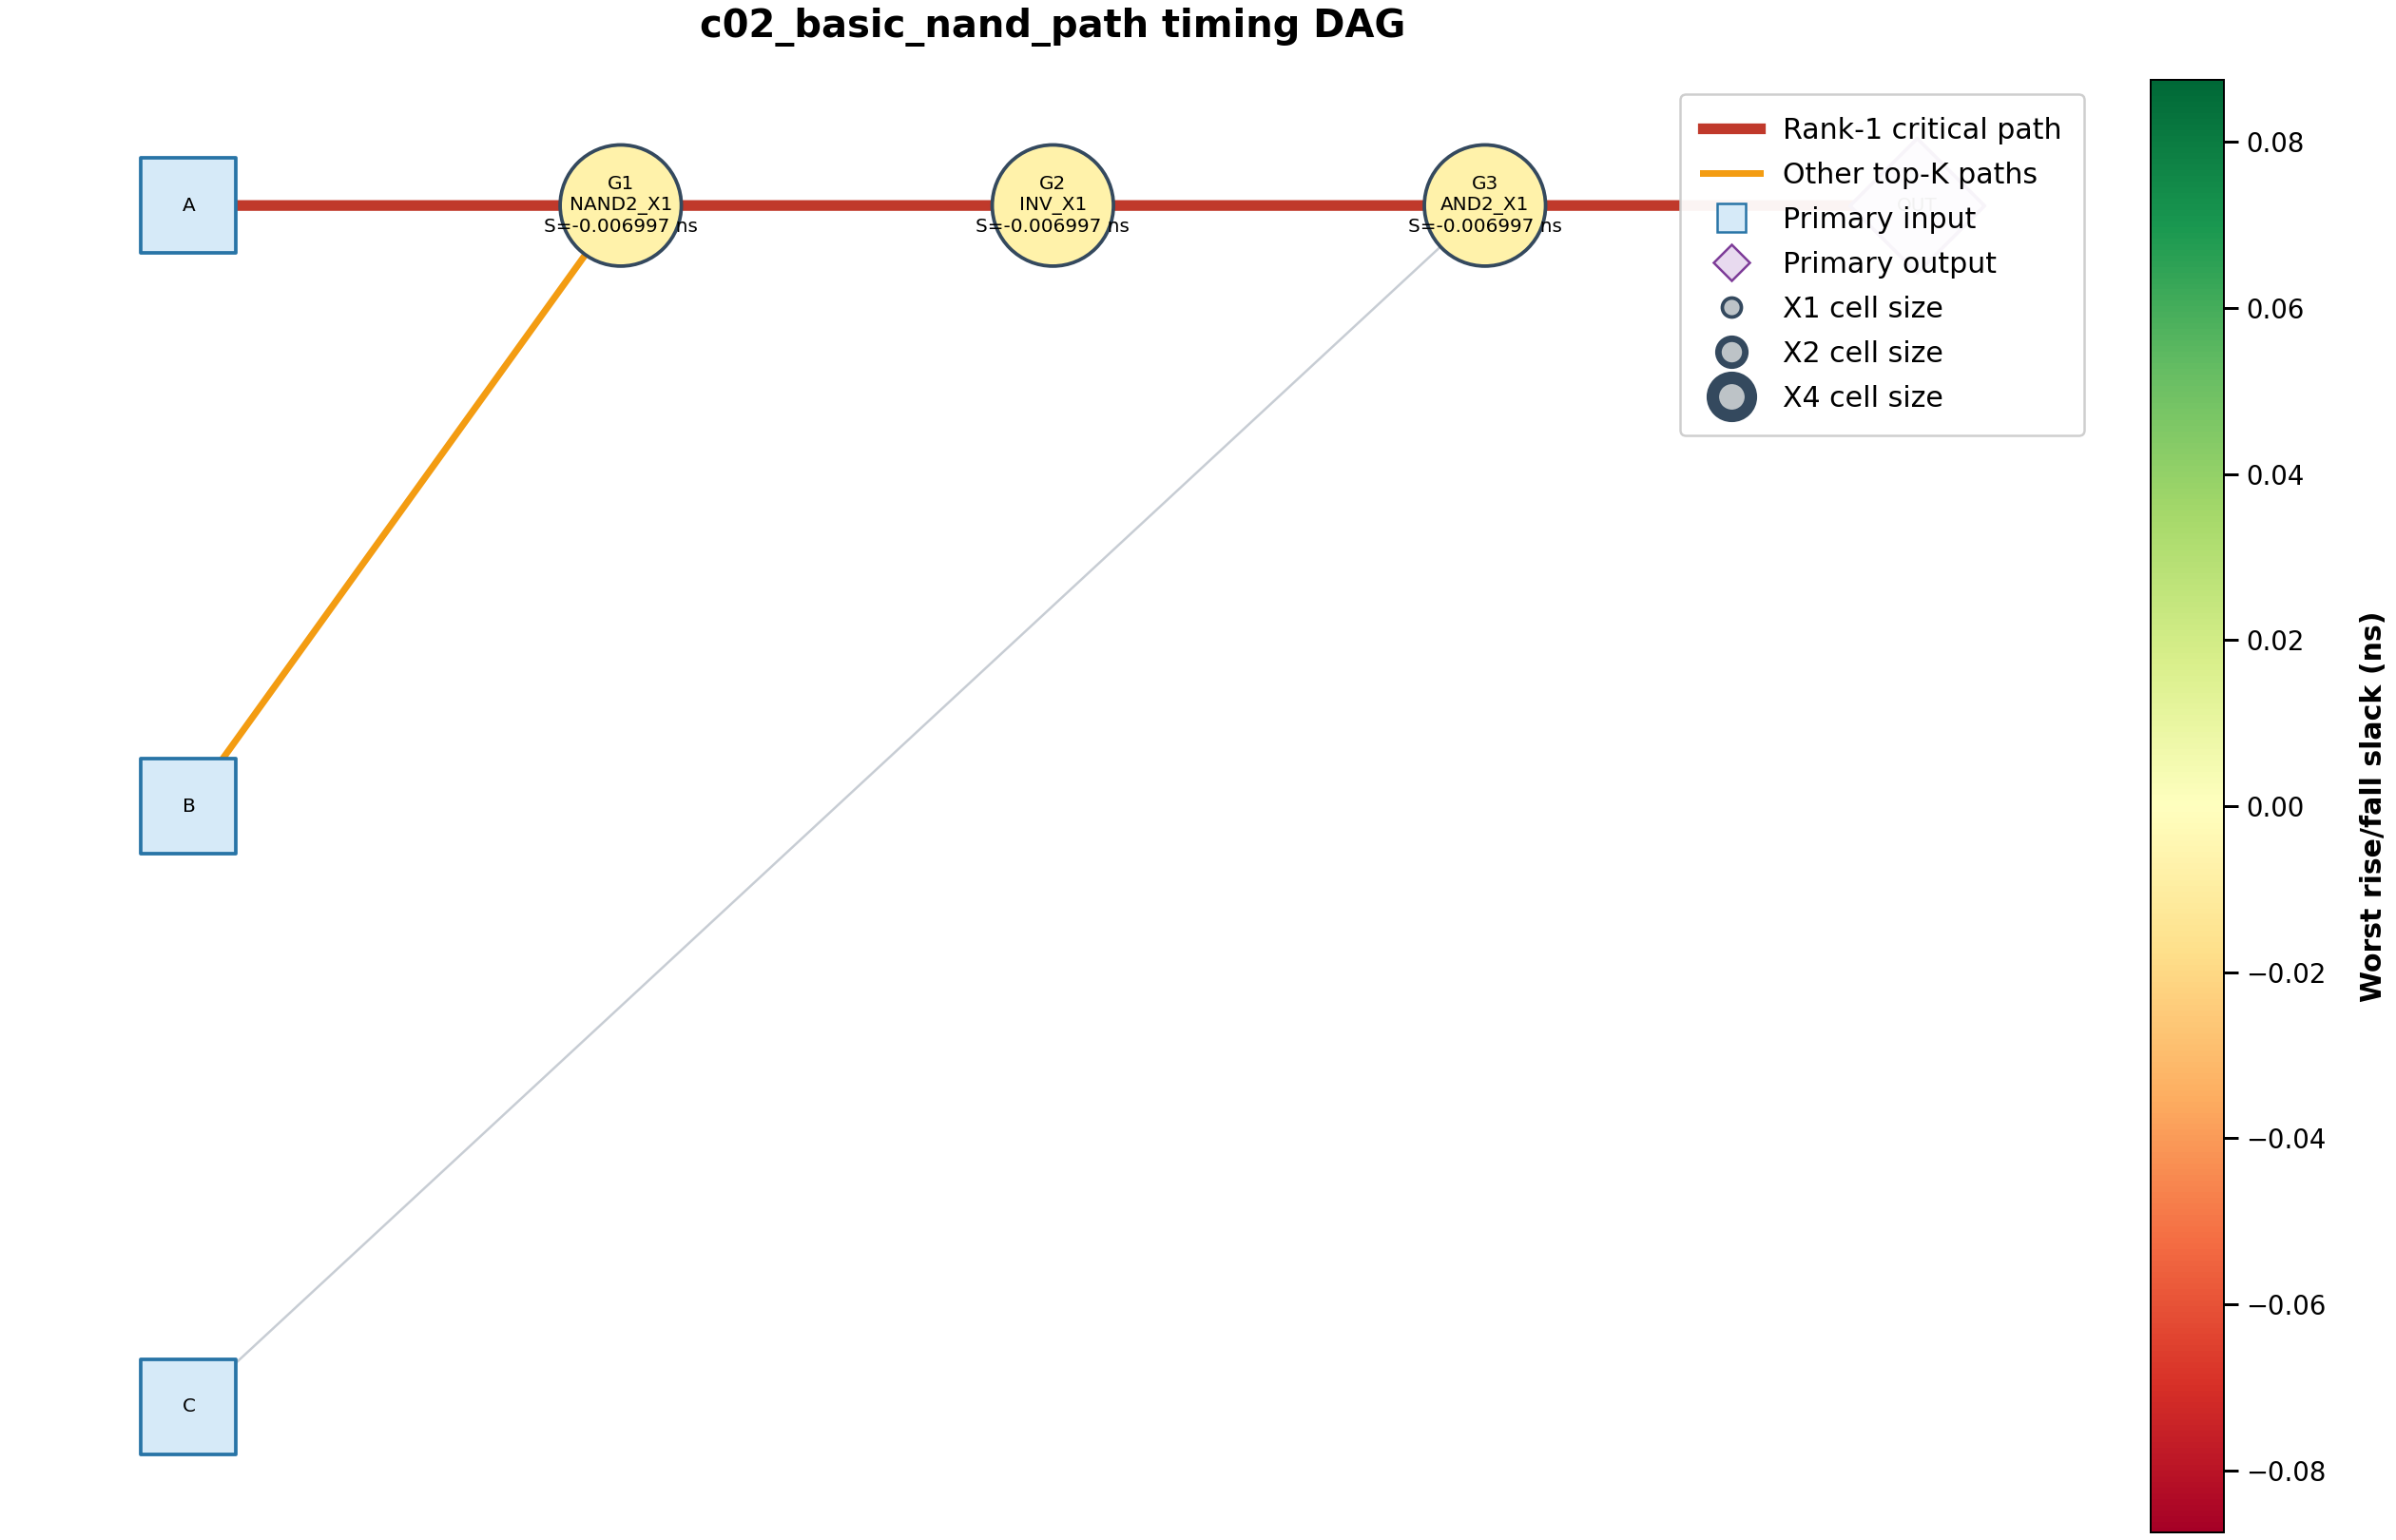
\includegraphics[width=0.92\textwidth]{c02_pre.png}
    \caption{\texttt{c02\_basic\_nand\_path}, pre-optimization. Nodes are
    colored by slack; the critical path is highlighted.}
    \label{fig:c02-pre}
\end{figure}

\begin{figure}[H]
    \centering
    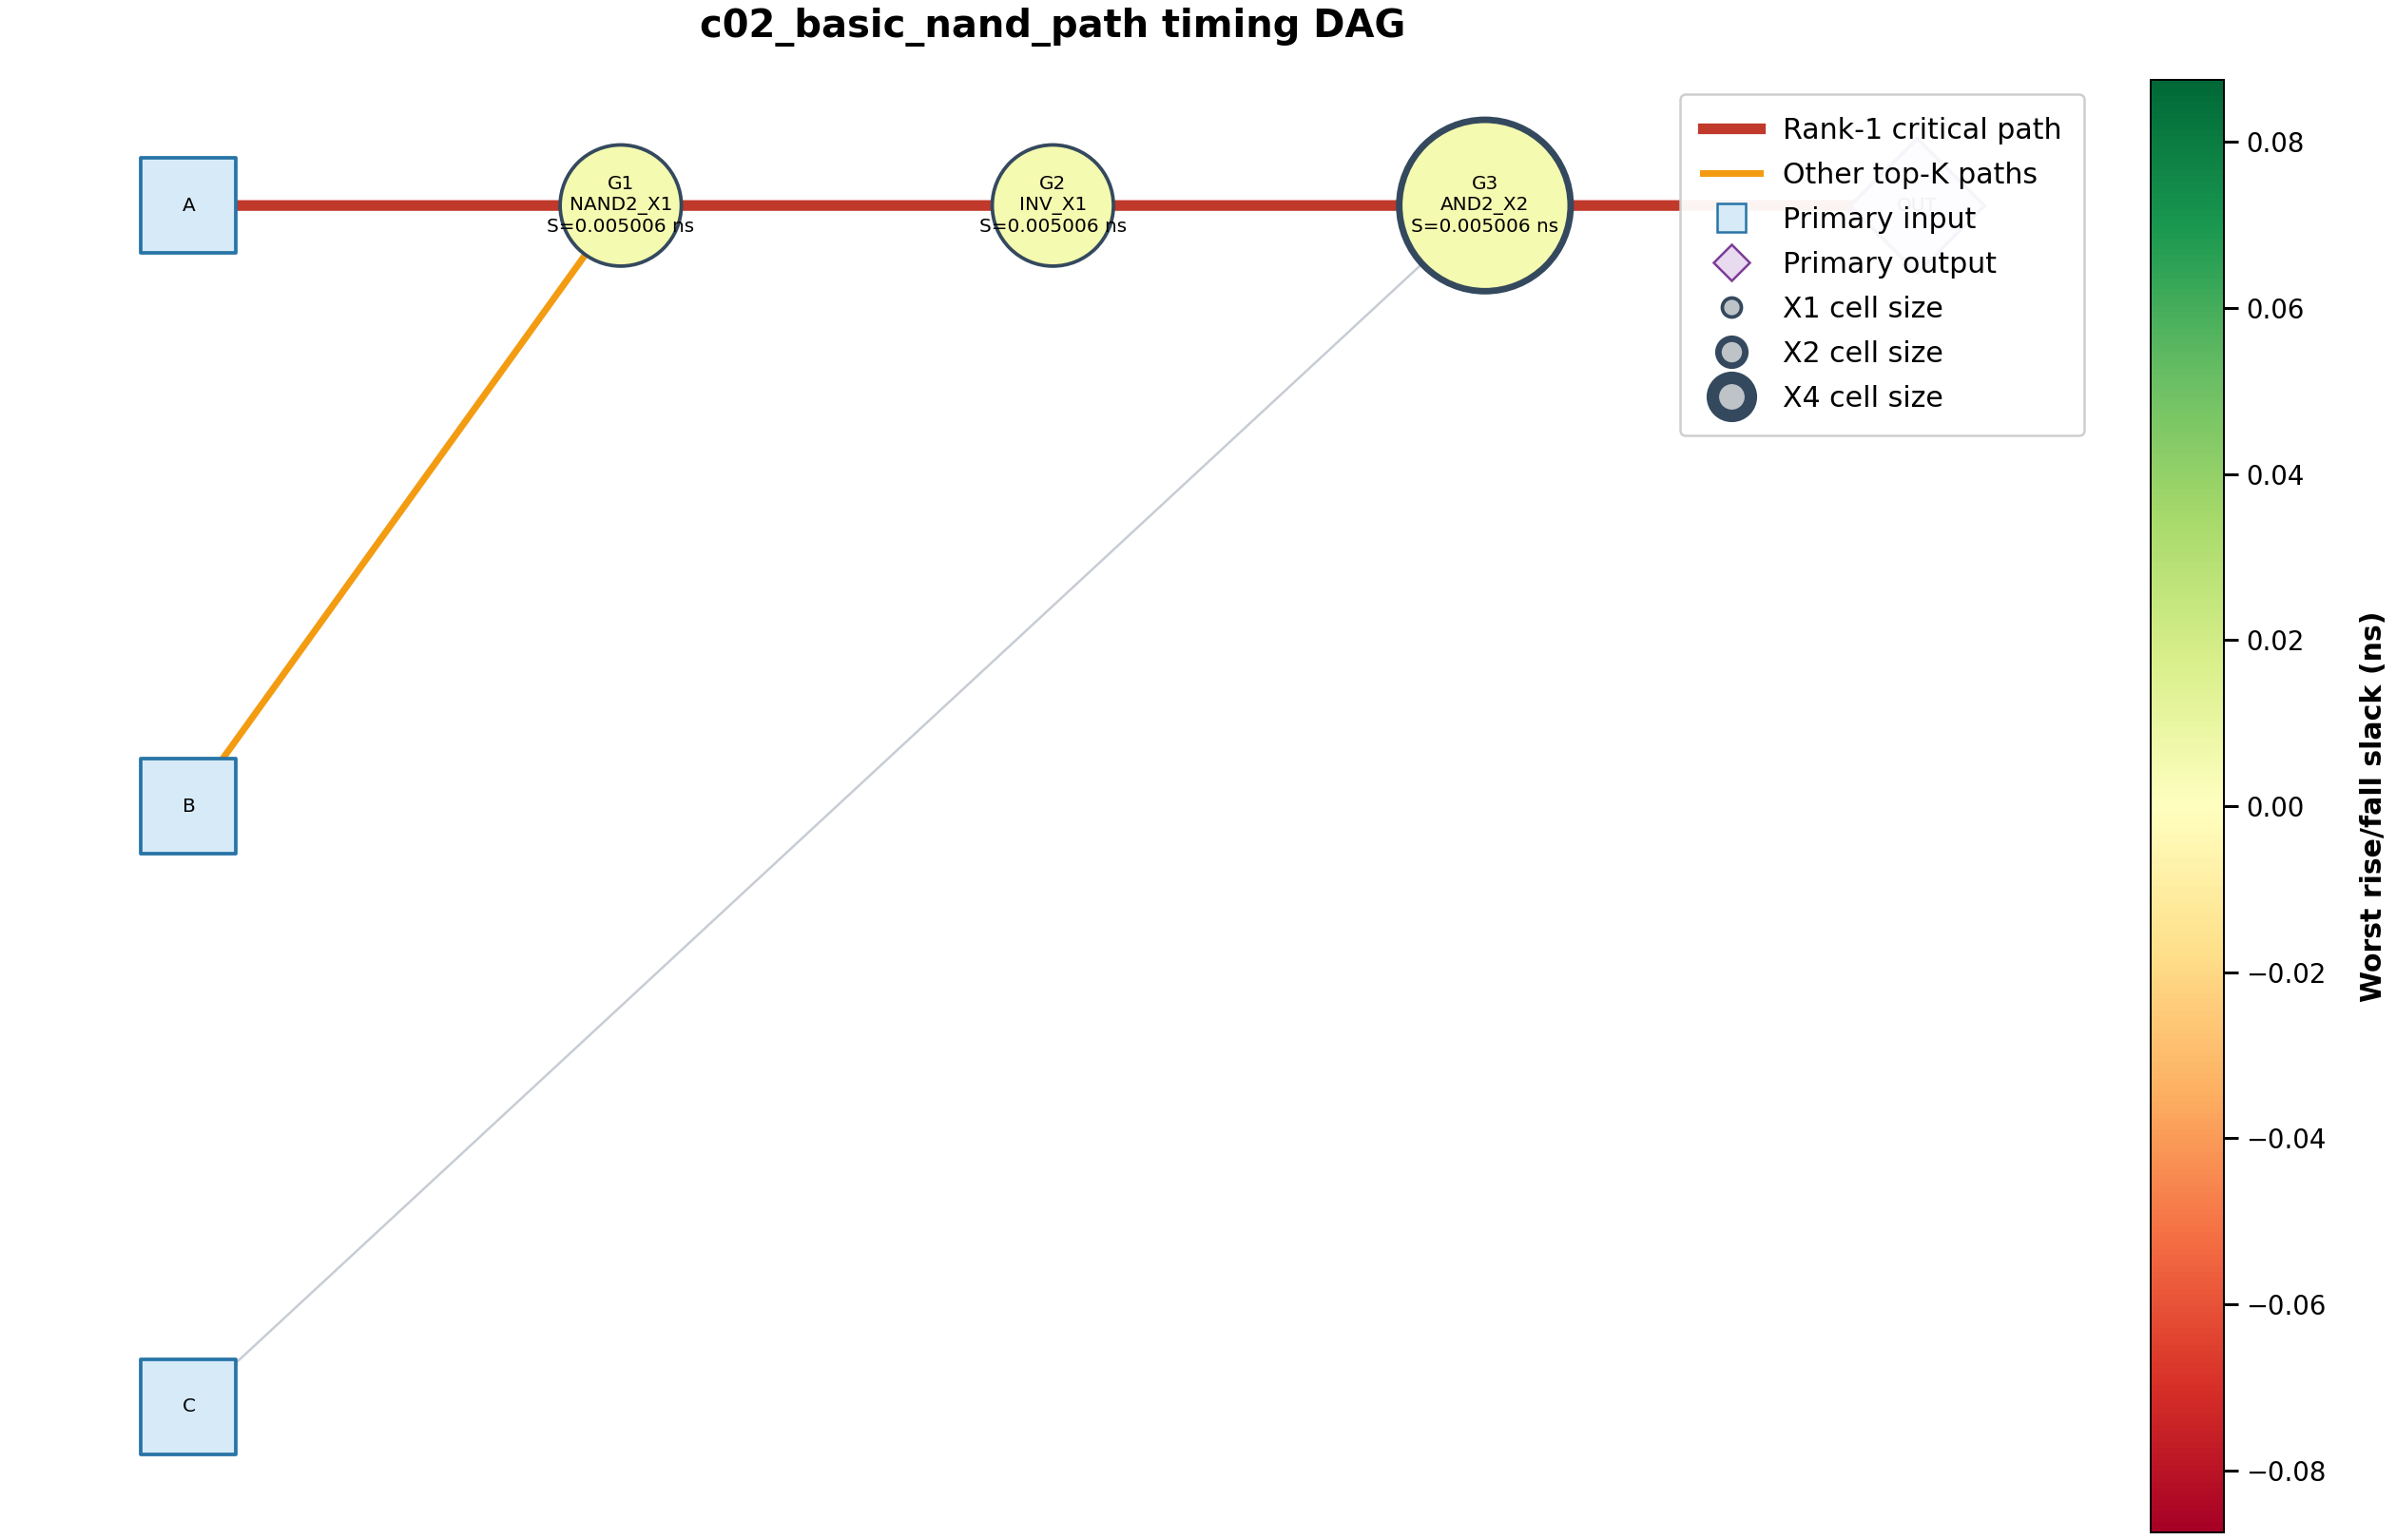
\includegraphics[width=0.92\textwidth]{c02_post.png}
    \caption{\texttt{c02\_basic\_nand\_path}, post-optimization (canonical
    slack-weighted-capacitance heuristic). Gate \texttt{G3} has been
    resized from \texttt{AND2\_X1} to \texttt{AND2\_X2}, resolving the
    timing violation.}
    \label{fig:c02-post}
\end{figure}

\Cref{fig:c02-convergence} makes the same story visible directly as a
convergence trace: slack-weighted capacitance (blue) reaches zero TNS and
positive WNS in a single accepted step and holds there, while random
greedy (green) needs two accepted steps to make partial progress and never
crosses zero. \Cref{fig:c02-outcomes} summarizes the same run as final
outcomes --- note criticality effort gap (orange) is visually
indistinguishable from slack-weighted capacitance on this particular
circuit, since both happen to find the same \texttt{G3} fix, consistent
with \cref{tab:res-heuristics}.

\begin{figure}[H]
    \centering
    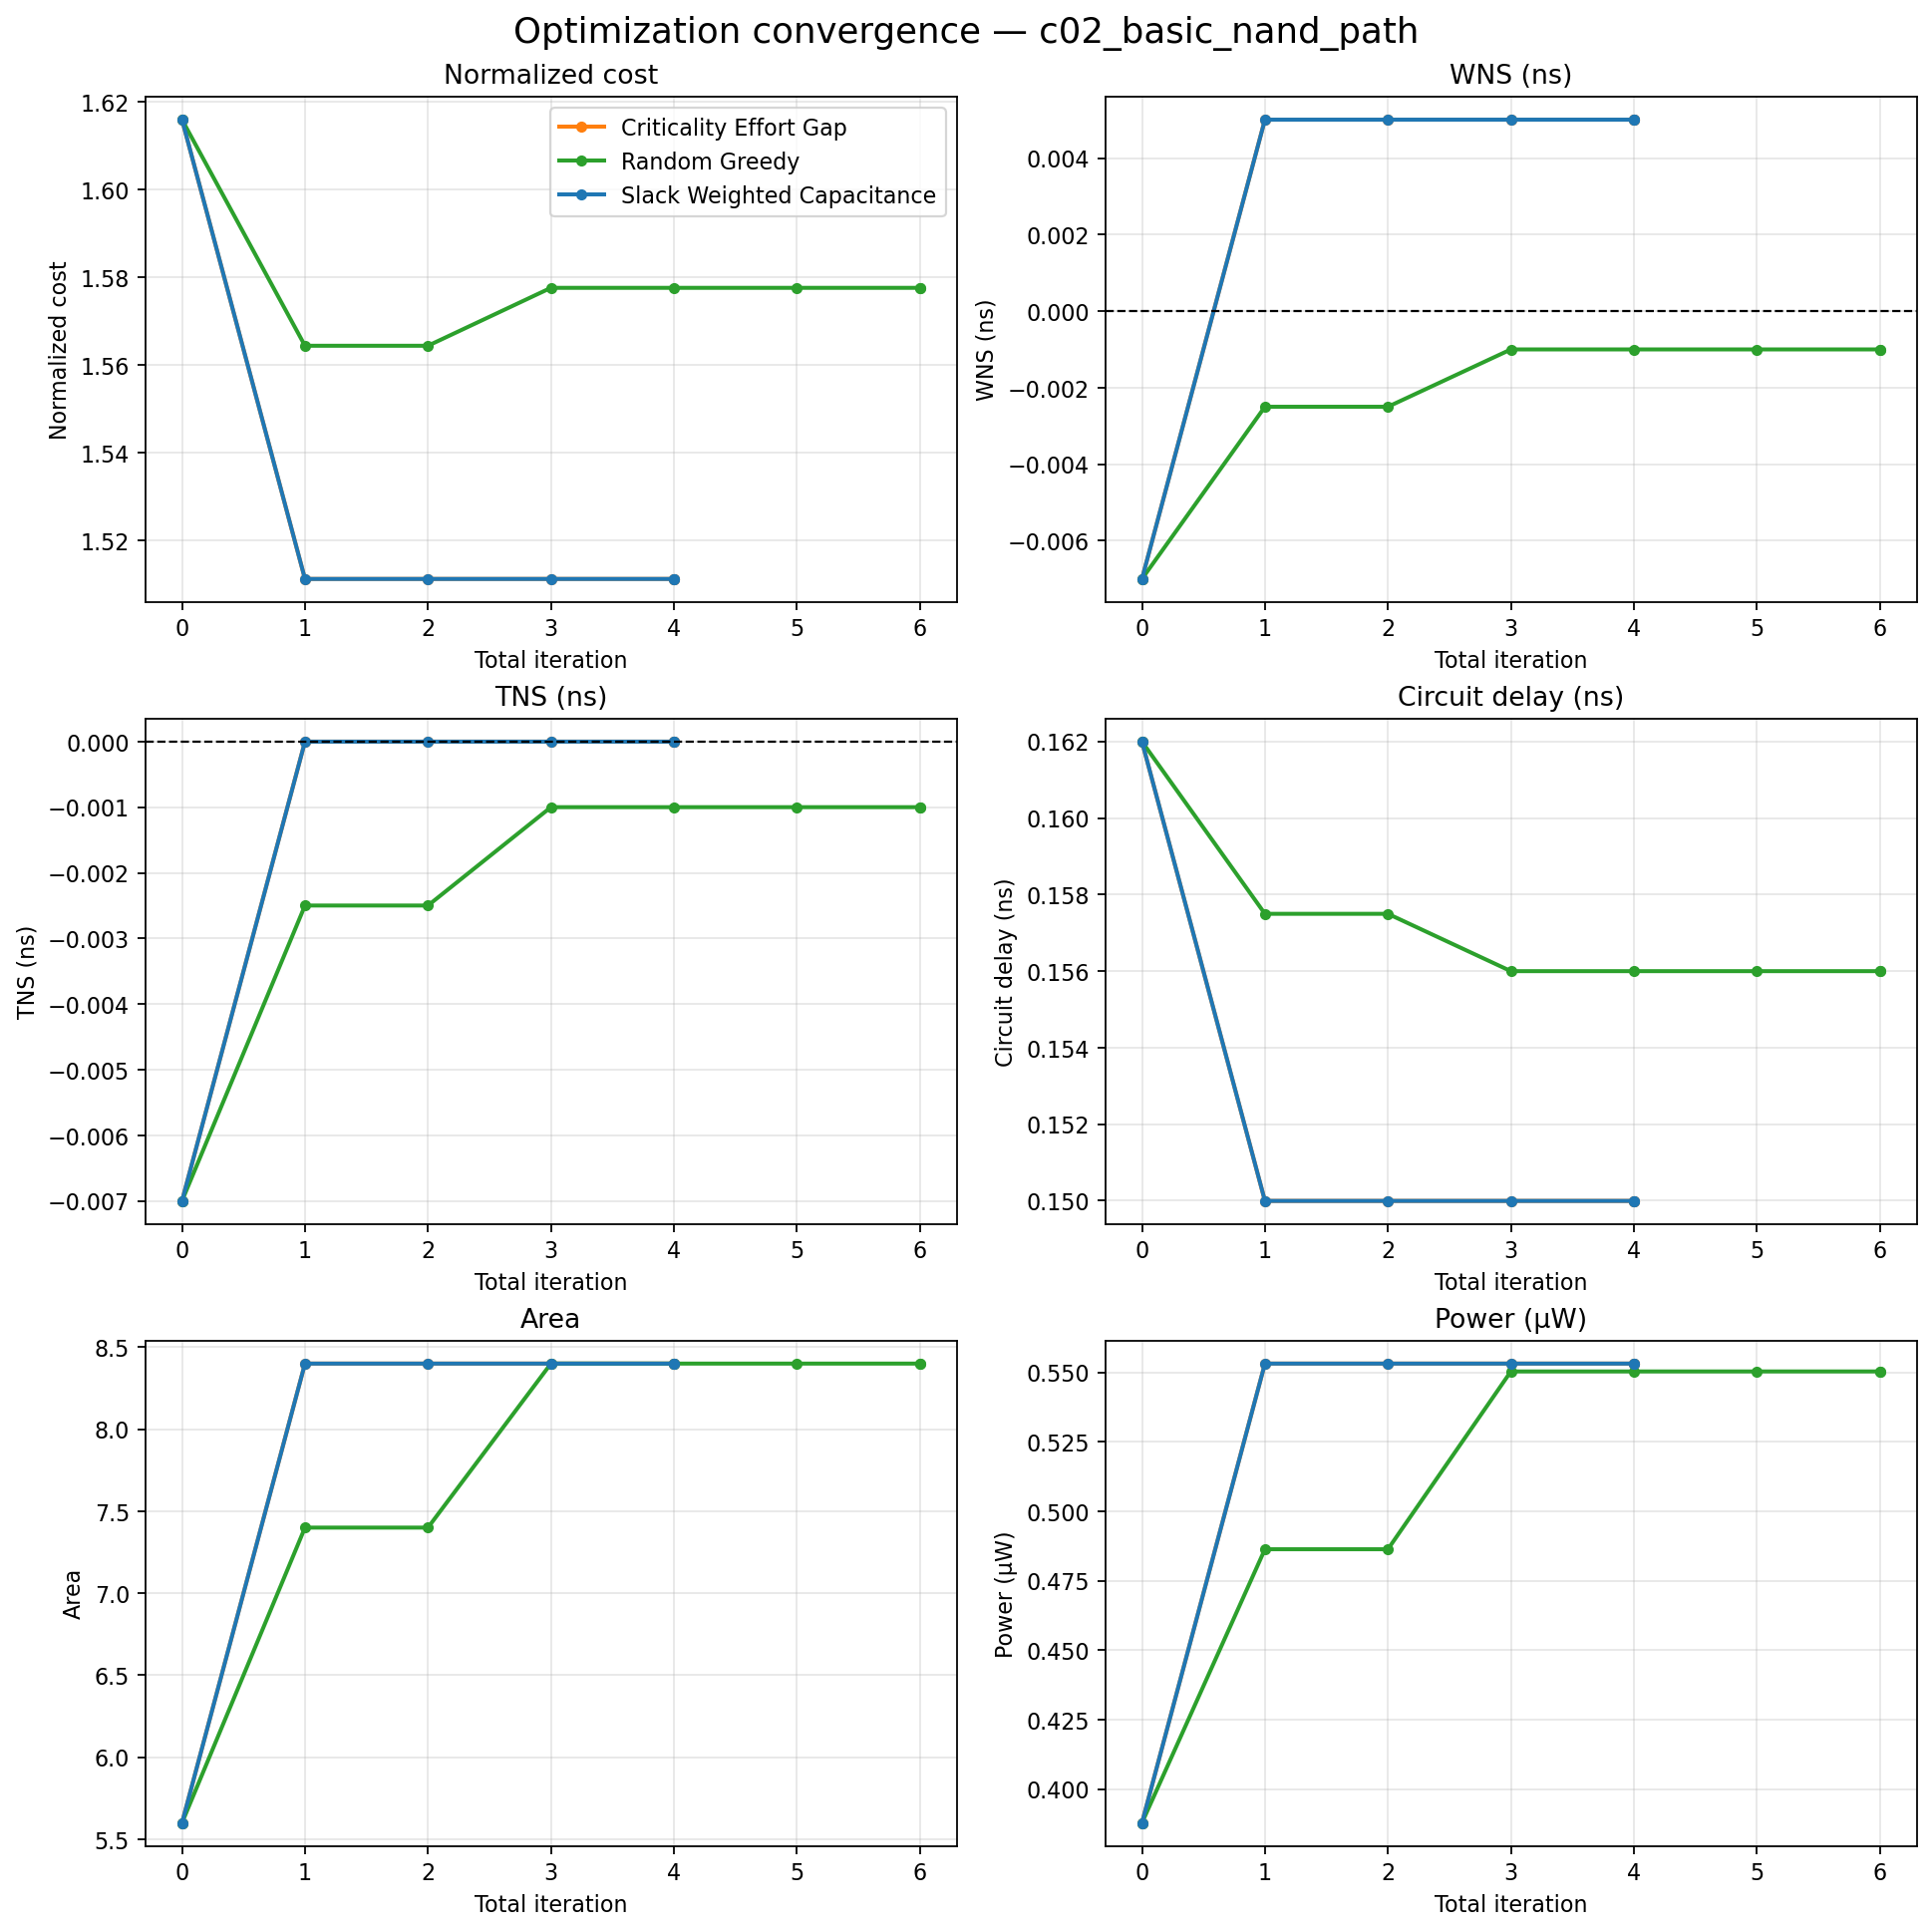
\includegraphics[width=\textwidth]{c02_basic_nand_path_conv.png}
    \caption{\texttt{c02\_basic\_nand\_path}: normalized cost, WNS, TNS,
    circuit delay, area, and power versus accepted-change iteration, for
    all three sequential heuristics (\cref{sec:opt-heuristics}). The
    horizontal dashed line marks the compliance threshold on the WNS/TNS
    panels.}
    \label{fig:c02-convergence}
\end{figure}

\begin{figure}[H]
    \centering
    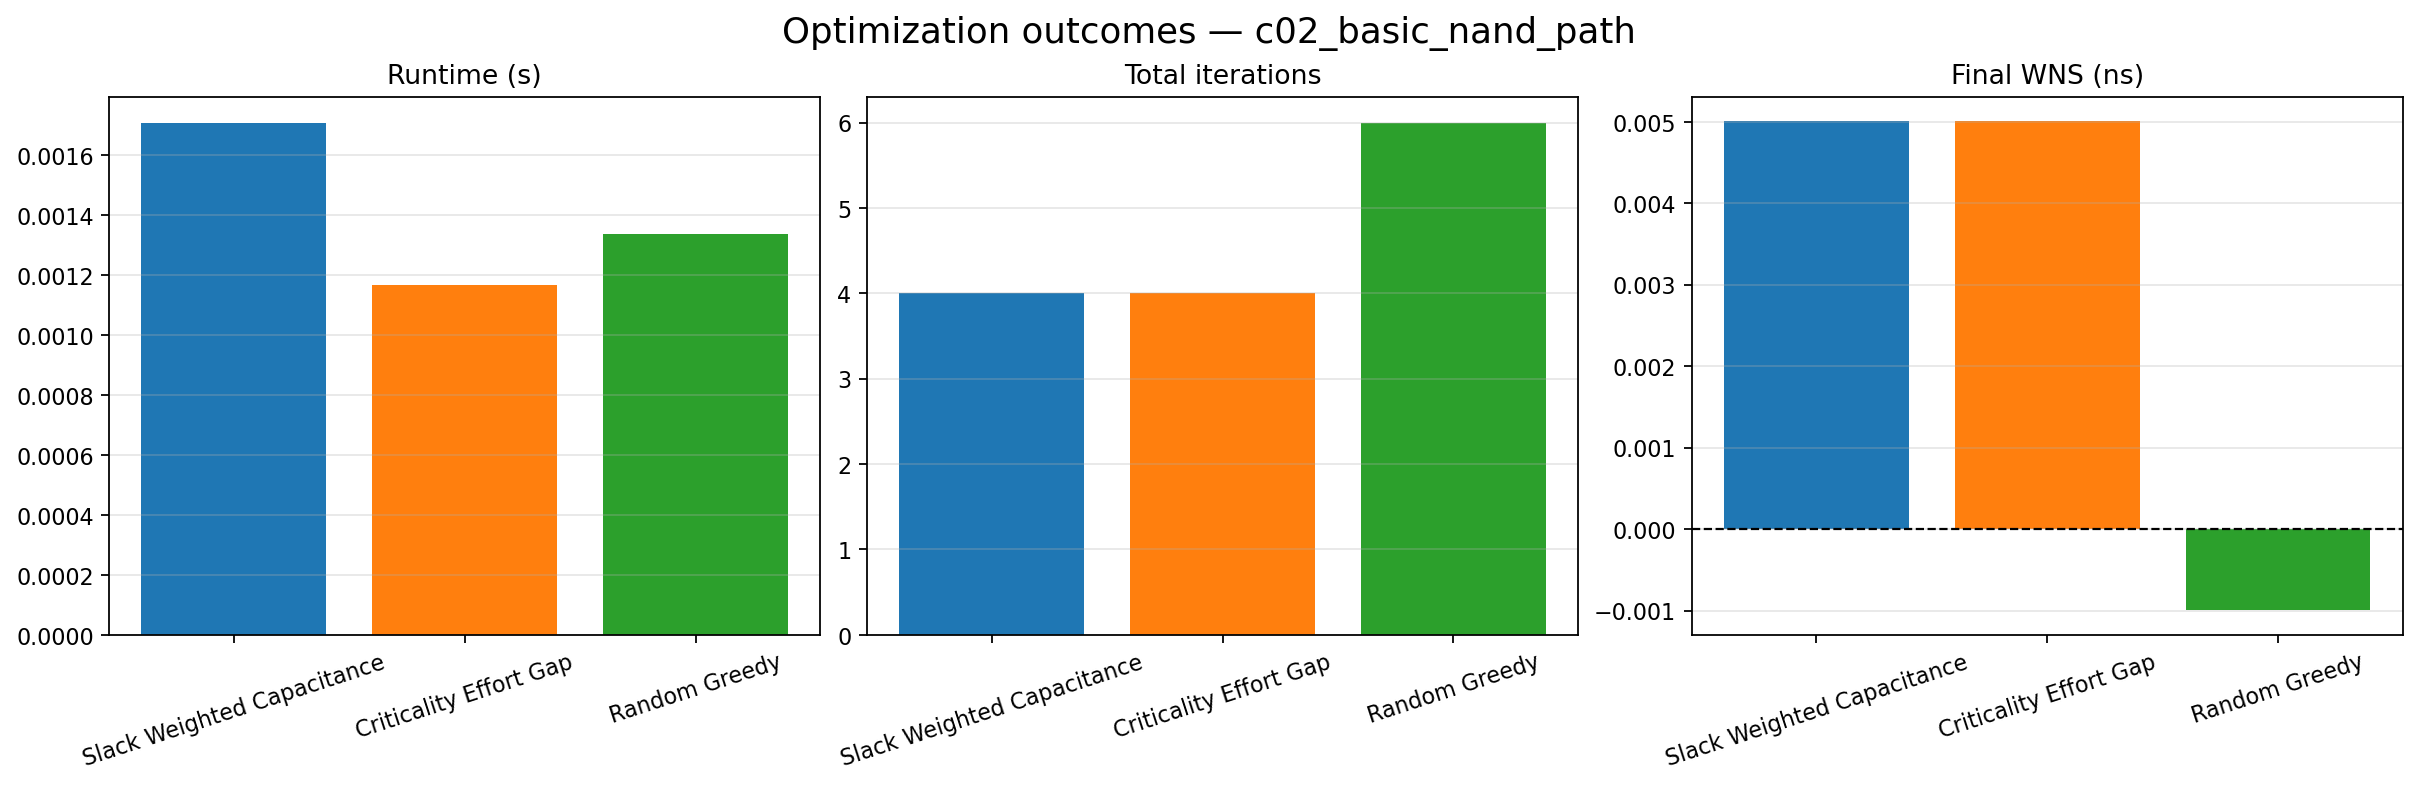
\includegraphics[width=\textwidth]{c02_basic_nand_path_outc.png}
    \caption{\texttt{c02\_basic\_nand\_path}: final runtime, total
    iterations (accepted and rejected attempts combined), and final WNS
    per heuristic.}
    \label{fig:c02-outcomes}
\end{figure}

\subsection{Case Study: Divergence Between the Two Logical-Effort Heuristics}
\label{sec:res-case-divergence}

\code{c13\_large\_reconvergent\_network} (74 gates) is the one circuit in
the suite on which slack-weighted capacitance and criticality effort gap
disagree, and the recorded iteration logs make the mechanism traceable
precisely rather than merely observable in the final numbers.

Criticality effort gap's search accepts exactly one change: at iteration 7,
\code{G65: OR2\_X1}\newline $\rightarrow$\code{OR2\_X2} is accepted under the
\emph{tied-WNS, TNS-improves} clause of the timing-repair acceptance rule
(\cref{sec:opt-accept}) --- WNS is left exactly unchanged at
$-0.0293$~ns, while TNS improves substantially, from $-0.2133$ to
$-0.1717$~ns. Eleven iterations later, at iteration 18, it proposes
\code{G7: NOR3\_X1}$\rightarrow$\code{NOR3\_X2} --- a resize that,
critically, \emph{is} available to criticality effort gap, since it is a
plain one-step-up candidate, not something requiring the logical-effort
bracket --- but this candidate is now \textbf{rejected} with reason
\emph{``candidate violates area or power constraints''}: the area consumed
by the earlier \code{G65} change has left no further budget for it. No
subsequent candidate improves WNS or TNS either, and the search terminates
\code{no\_feasible\_change} with the circuit still at its original
$-0.0293$~ns violation.

Slack-weighted capacitance's search proposes that exact same
\code{G7: NOR3\_X1}$\rightarrow$\code{NOR3\_X2} resize much earlier, at
iteration 13, while the circuit is still at its pristine initial area
budget (its own higher-scored earlier candidates were all rejected
outright rather than accepted, so no budget had yet been spent). At that
point it is well within budget and is accepted, cutting the violation's
magnitude by \textbf{88.6\%} ($-0.0293\rightarrow-0.0033$~ns); a second
accepted change at
iteration 35, \code{G6: NAND3\_X1}$\rightarrow$\code{NAND3\_X2}, then
closes the remaining gap entirely ($\mathrm{WNS}\rightarrow+0.0037$~ns,
$\mathrm{TNS}\rightarrow 0$).

This is a second, independent confirmation of the same effect identified
in \cref{sec:res-case-c02}: the outcome is decided not by what a heuristic
is theoretically permitted to consider --- both heuristics have \code{G7}
available --- but by whether an earlier accepted change quietly consumes
budget that a later, more consequential change will need. In this instance
the effect is sharper than in the c02 case study, because
criticality effort gap's early accepted change is not even a step toward
resolving the violation directly (it is WNS-neutral, accepted purely for a
TNS improvement); slack-weighted capacitance's higher-scored ranking
happens to defer any budget-consuming change until the one that actually
matters, avoiding the trap entirely on this circuit.

\Cref{fig:c13-convergence} shows this divergence directly: the orange
(criticality effort gap) trace visibly plateaus at a still-negative WNS
after its single early step, its cost curve flattening well above the blue
(slack-weighted capacitance) trace, which instead makes a late but decisive
descent to full compliance once its own higher-ranked candidates ahead of
\texttt{G7} are exhausted.

\begin{figure}[H]
    \centering
    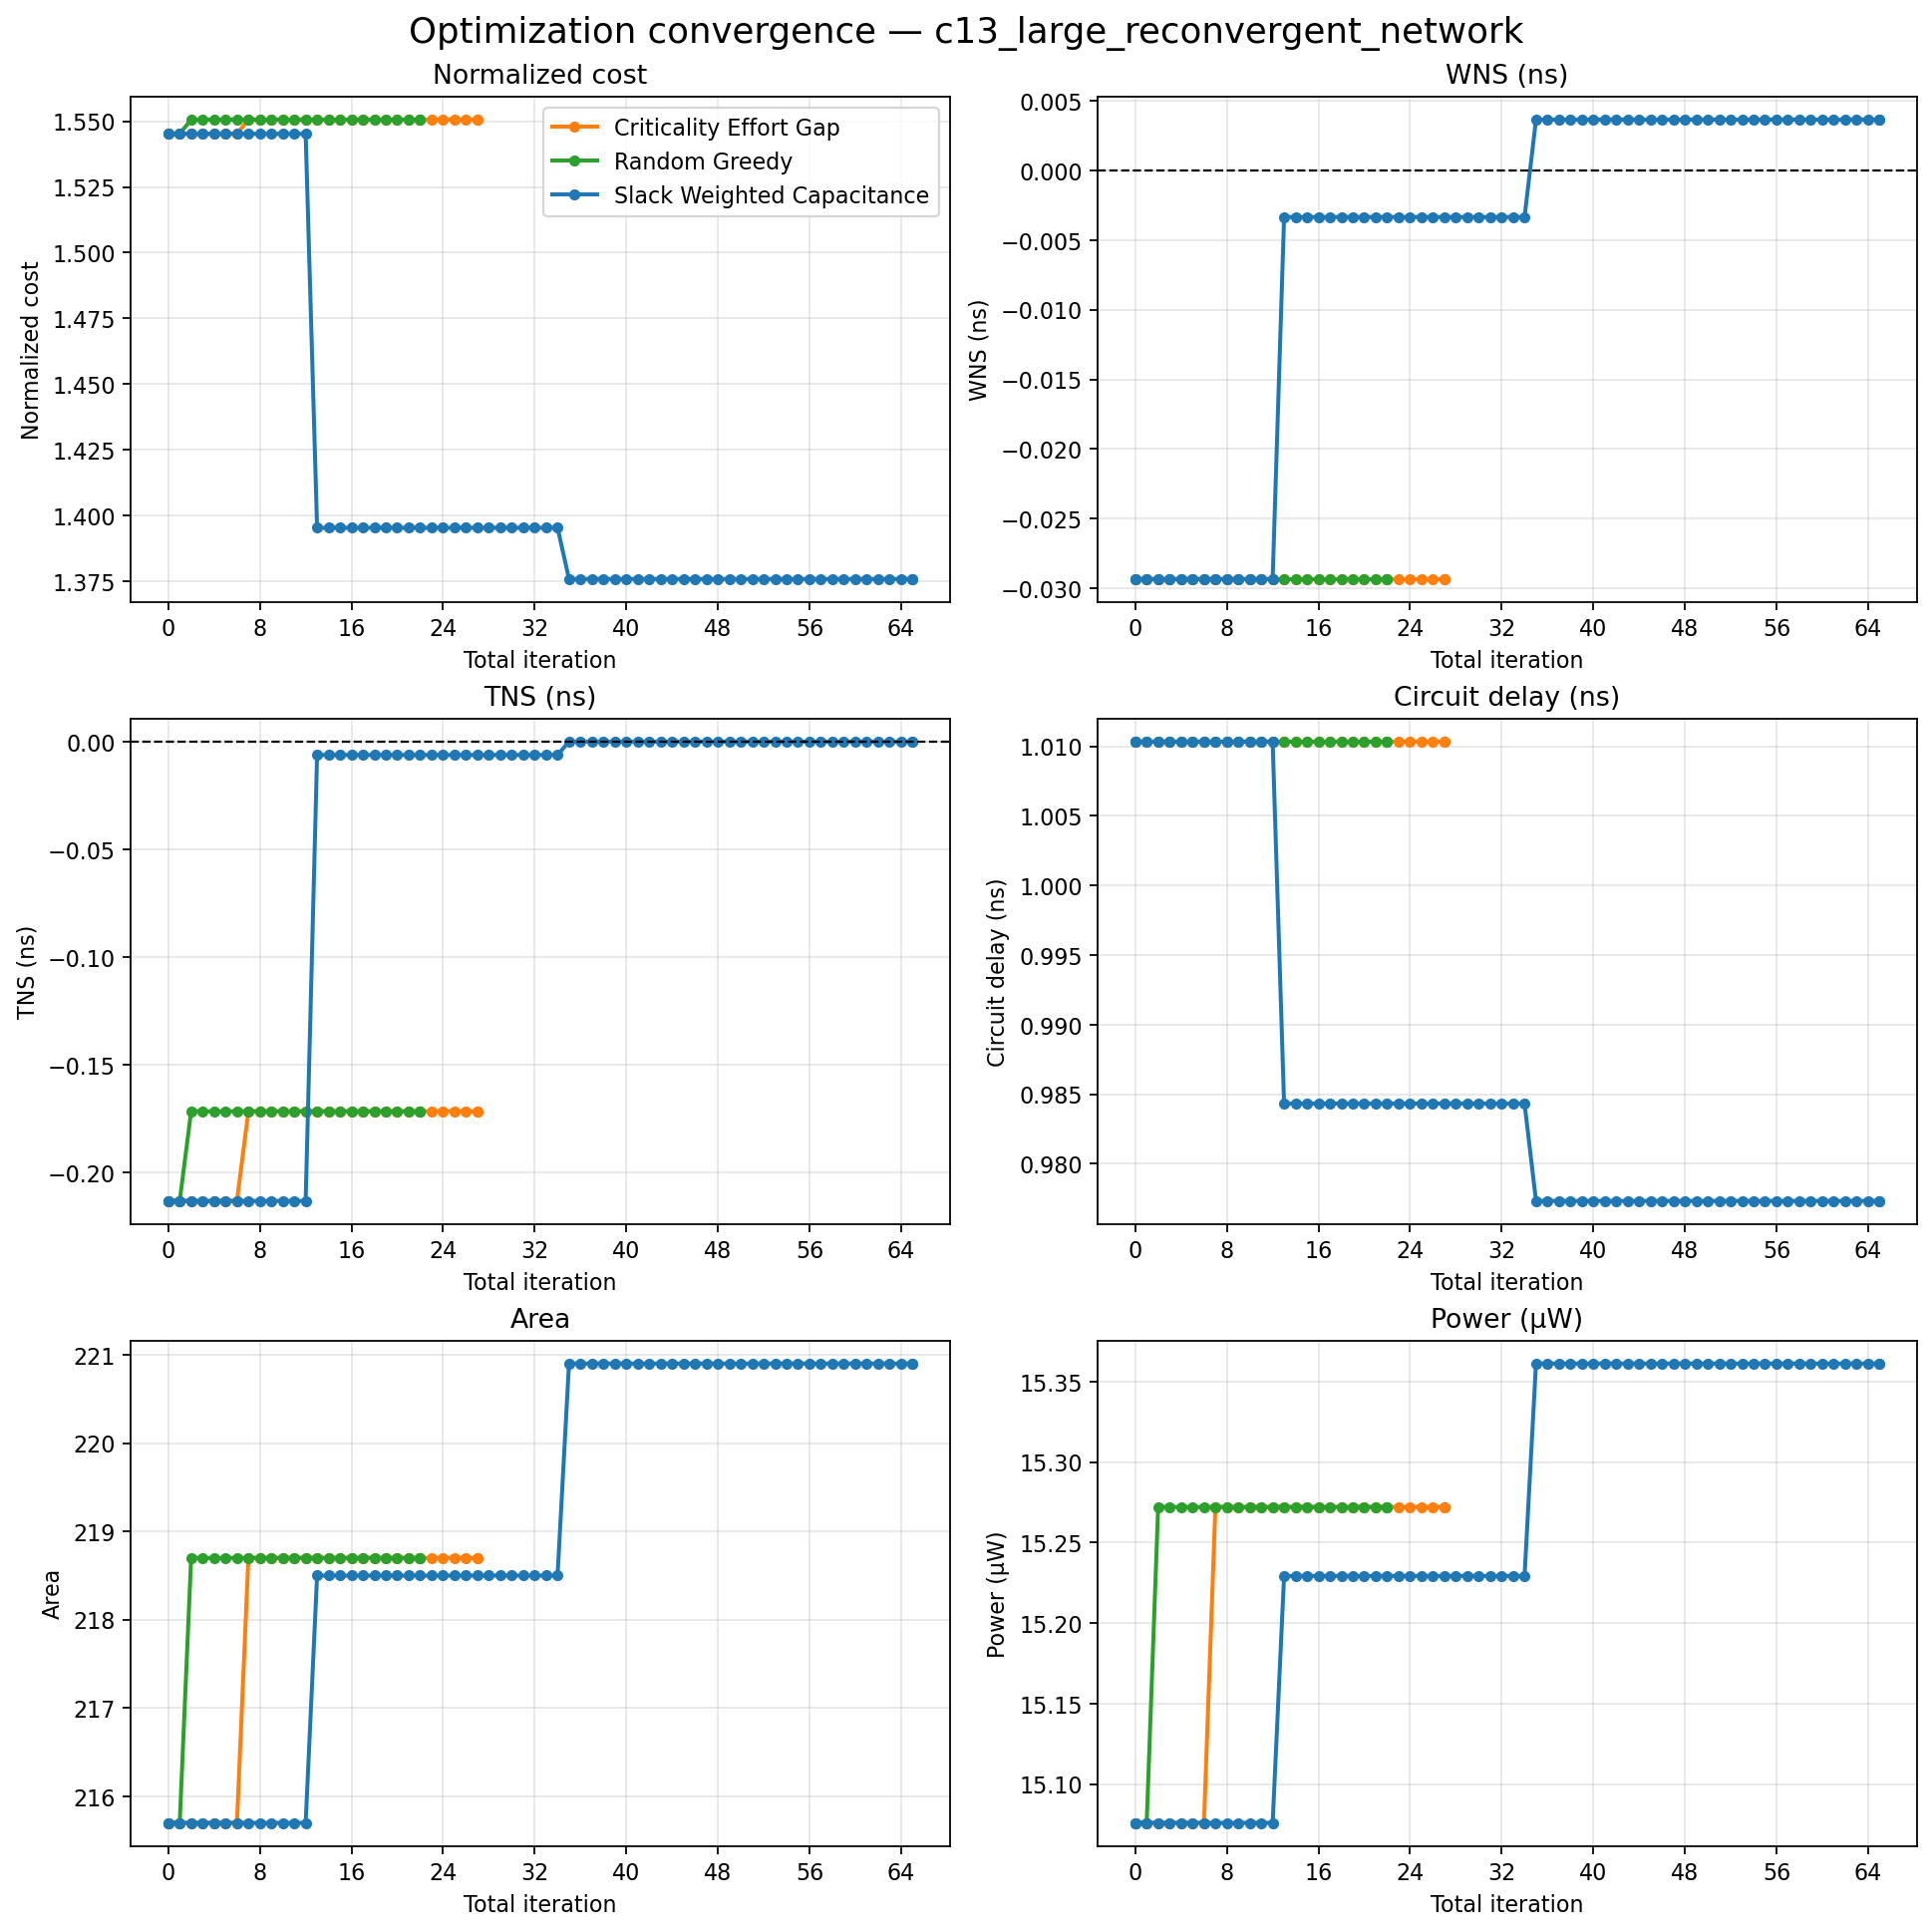
\includegraphics[width=\textwidth]{c13_large_reconvergent_network_conv.png}
    \caption{\texttt{c13\_large\_reconvergent\_network}: convergence trace
    for all three sequential heuristics. Criticality effort gap's single
    early, WNS-neutral step (\cref{sec:res-case-divergence}) is visible as
    the orange trace's premature plateau above zero WNS.}
    \label{fig:c13-convergence}
\end{figure}

\section{Monte Carlo Statistical Analysis: \texttt{c12\_monte\_carlo\_switching}}
\label{sec:res-montecarlo}

\Cref{tab:res-mc} reports the paired Monte Carlo comparison
(\cref{ch:monte-carlo}) for the one benchmark circuit with statistical
analysis enabled, using $M = 3000$ samples, $\sigma_g = 0.03$,
$\sigma_l = 0.05$, and random seed $1405$.

\begin{table}[H]
\centering
\small
\begin{tabular}{@{}lrr@{}}
\toprule
\textbf{Metric} & \textbf{Pre-optimization} & \textbf{Post-optimization} \\
\midrule
Mean circuit delay (ns) & 0.3194 & 0.3041 \\
Std.\ dev.\ circuit delay (ns) & 0.0124 & 0.0116 \\
Mean WNS (ns) & -0.0044 & \phantom{-}0.0109 \\
Violation probability & 0.631 & 0.174 \\
Timing yield & 0.369 & 0.826 \\
Modal critical path (probability) & \parbox[t]{4.1cm}{\raggedright \texttt{D->G4->G5->G6->G7} (0.606)} & \parbox[t]{4.1cm}{\raggedright \texttt{A->G1->G2->G3->G7} (0.628)} \\
\bottomrule
\end{tabular}
\caption{Paired Monte Carlo statistical timing comparison, pre- versus
post-optimization, \texttt{c12\_monte\_carlo\_switching}, $M=3000$ samples.}
\label{tab:res-mc}
\end{table}

Optimization improves timing yield from \textbf{36.9\% to 82.6\%} --- a
$+45.7$ percentage-point improvement --- confirming that the
nominal-corner WNS improvement reported in \cref{sec:res-heuristics} for
this circuit translates into a substantial improvement in robustness to
manufacturing variation, not merely a nominal-case artifact. Notably, the
\emph{identity} of the modal critical path also changes: under process
variation, the pre-optimization design is most often limited by the path
through \code{G4--G7} (driven by primary input \code{D}), while the
post-optimization design is most often limited by an entirely different
path through \code{G1--G3, G7} (driven by primary input \code{A}) --- the
sizing changes did not merely widen the margin on the original critical
path, they shifted which path is critical at all, which is exactly the
kind of effect a single nominal-corner STA run cannot reveal.

\section{Synthetic Benchmark Suite Results}
\label{sec:res-benchmarking}
 
This section reports results from \code{complex\_repair\_suite}, a 60-case
synthetic benchmark generated and evaluated with the framework of
\cref{ch:benchmarking}. Unlike the fixed suite of \cref{sec:res-heuristics},
which compares three heuristics on fifteen circuits (eleven of them with only
a single-digit gate count), this suite is specifically configured to stress
the optimizer on large, structurally diverse circuits, and evaluates all
\textbf{four} heuristics --- including brute force, absent from the fixed
suite's reported comparison (\cref{sec:opt-bruteforce}) --- against the
independent counterfactual oracle of \cref{sec:bench-oracle}.
 
\subsection{Suite Composition and Generation Reliability}
\label{sec:res-bench-generation}

The suite comprises 60 cases: 40 procedurally generated (structured-random
topologies, 150--250 gates, 8--20 logic levels, targeting a
$0.35$ reconvergence probability and up to 6-way fan-out) and 20 seeded
from \code{c15\_high\_fanout\_sizing\_fabric} (\cref{sec:res-nominal}) under
independently sampled electrical conditions and planted mutations. Every
case's reference assignment was independently certified by an 8-restart,
beam-width-64 multi-start beam search (\code{best\_known\_multi\_start\_beam},
\cref{sec:bench-reference}) before any downsizing mutation was planted, and
each resulting initial (post-mutation) circuit was verified to have a
negative WNS strictly within the configured area/power budget.
 
Generation reliability was total for this run: of 60 requested cases, all
60 were generated successfully, with \textbf{zero} entries in
\code{generation\_failures.csv} --- every case succeeded on its first
generation attempt, with no discarded partial attempts of any kind.
 
\subsection{Wilson-Interval Repair Rate}
\label{sec:res-bench-repair-rate}
 
\Cref{tab:bench-repair-rate} reports the case-level repair rate for each
heuristic with a 95\% Wilson confidence interval (\cref{sec:bench-metrics}).
Brute force and random greedy are run once and 20 times per case
respectively (the latter to characterize its stochastic variance, per
\cref{sec:bench-parallel}); the two logical-effort-informed heuristics,
being deterministic given a fixed circuit and candidate order
(\cref{sec:opt-heuristics}), are run once per case.
 
\begin{table}[H]
\centering
\small
\begin{tabular}{@{}lrrrl@{}}
\toprule
\textbf{Heuristic} & \textbf{Runs} & \textbf{Successes} & \textbf{Repair rate} & \textbf{95\% Wilson CI} \\
\midrule
Brute force & 60 & 60 & 100.0\% & [93.98\%, 100.00\%] \\
Criticality effort gap & 60 & 60 & 100.0\% & [93.98\%, 100.00\%] \\
Slack-weighted capacitance & 60 & 59 & 98.3\% & [91.14\%, 99.71\%] \\
Random greedy & 1200 & 1134 & 94.5\% & [93.06\%, 95.65\%] \\
\bottomrule
\end{tabular}
\caption{Case-level repair rate with 95\% Wilson confidence intervals (60 cases; random greedy evaluated with 20
repetitions per case, 1200 total runs).}
\label{tab:bench-repair-rate}
\end{table}
 
\begin{figure}[H]
    \centering
    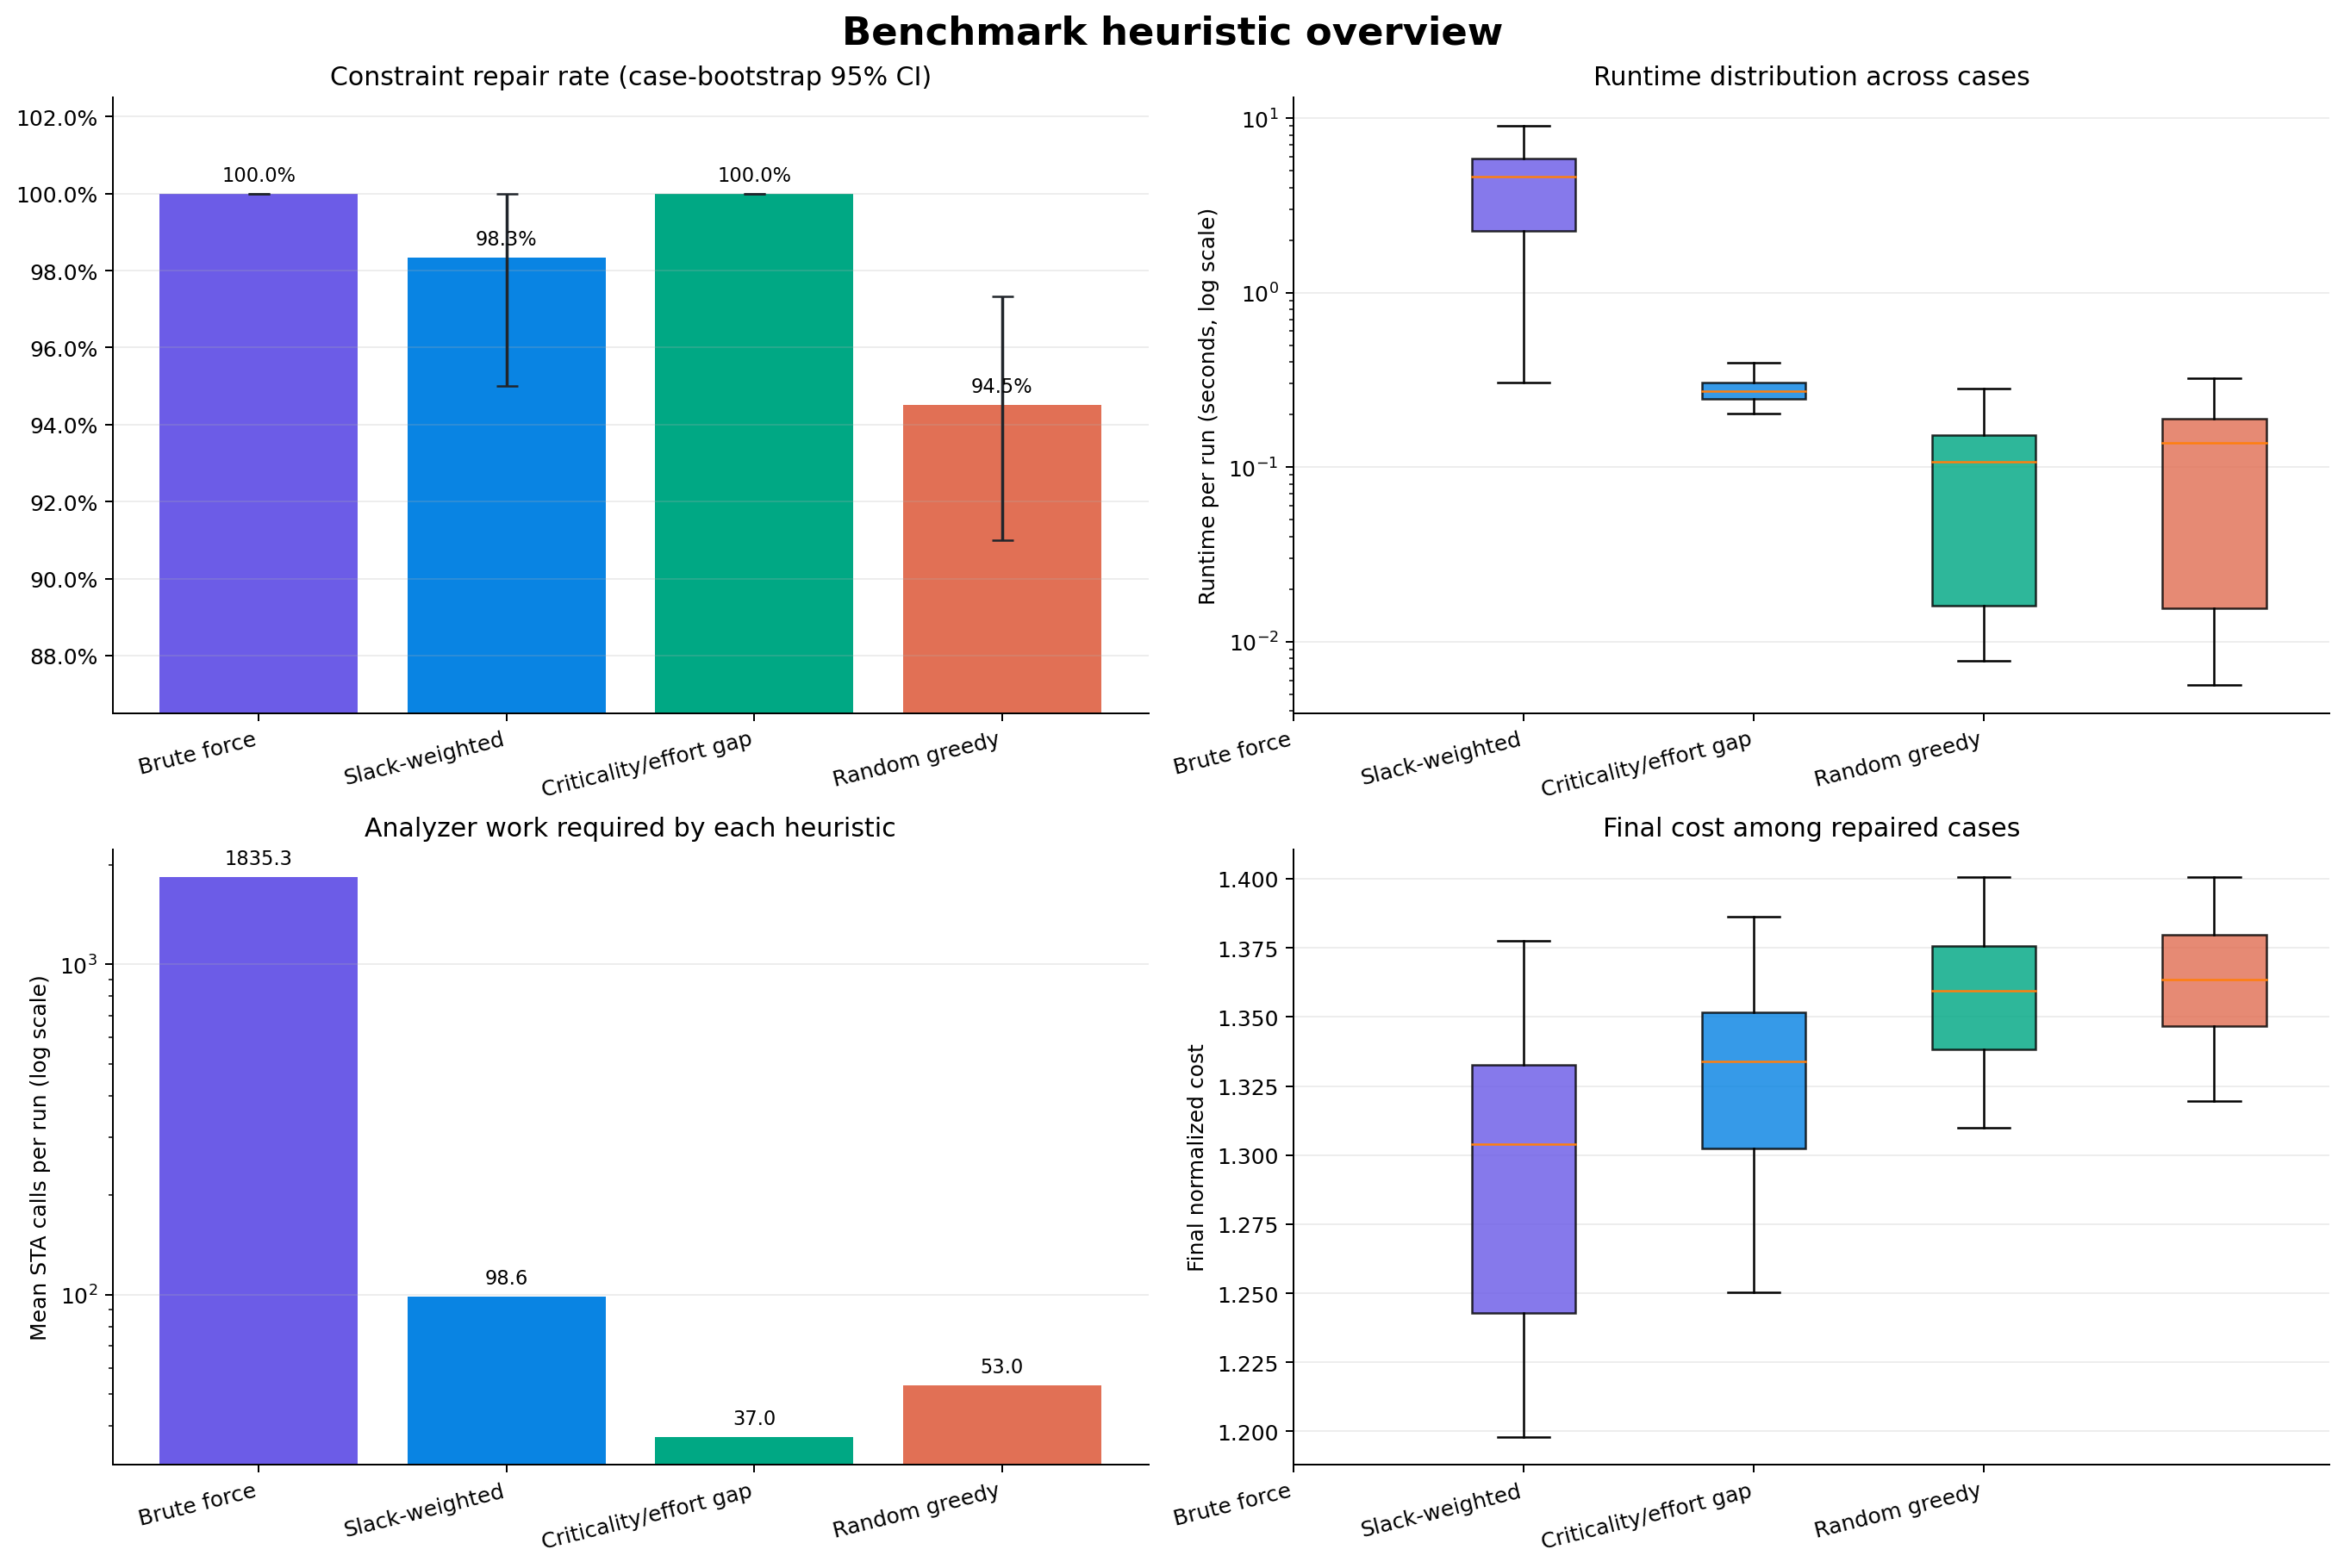
\includegraphics[width=\textwidth]{benchmarking/heuristic_overview.png}
    \caption{Benchmark heuristic overview: repair rate with 95\% bootstrap
    confidence intervals, per-run wall-clock runtime distribution, mean STA
    calls per run (log scale), and final normalized cost among repaired
    cases only. Note the four-order-of-magnitude STA-call gap between
    brute force ($\approx 1835$ calls/run) and criticality effort gap
    ($\approx 37$ calls/run).}
    \label{fig:bench-heuristic-overview}
\end{figure}
 
Three results are worth drawing out beyond the headline repair rates.
First, criticality effort gap matches brute force's 100\% repair rate on
this suite exactly, and does so at $\approx 37$ mean STA calls per run
versus brute force's $\approx 1835$ --- a two-order-of-magnitude reduction
in search cost for an identical repair outcome on this population. Second,
slack-weighted capacitance --- the heuristic found strictly more reliable
than criticality effort gap on the fixed suite (\cref{sec:res-heuristics},
where it alone repaired \code{c13\_large\_reconvergent\_network}) --- is
here the \emph{less} reliable of the two logical-effort-informed
heuristics, with a single failure among its 60 cases. This is a genuine,
population-dependent reversal, not a contradiction: the fixed suite's
one divergence case (\cref{sec:res-case-divergence}) is a single 74-gate
circuit, and this suite's 60 cases, averaging $150$--$250$ gates, are a
different and much larger sample; a report should not extrapolate either
suite's heuristic ranking to circuits outside its own tested population.
Third, random greedy's 1200-run aggregate repair rate (94.5\%) sits
noticeably below its \emph{best-run} behavior implied by
\cref{fig:bench-case-reliability} below --- most of its failures are
concentrated in specific cases, not spread uniformly across the suite.
 
The single slack-weighted-capacitance failure is traceable to a specific
case: \code{case\_0032} (198 gates, 18 logic levels, 7 primary inputs, 8
primary outputs, initial $\mathrm{WNS}=-0.0357$~ns, reference
$\mathrm{WNS}=+0.0051$~ns). Both brute force ($\mathrm{WNS}=+0.0028$~ns)
and criticality effort gap ($\mathrm{WNS}=+0.0051$~ns, matching the
reference exactly) repair this case; slack-weighted capacitance terminates
\code{no\_feasible\_change} at $\mathrm{WNS}=-0.0003$~ns --- a residual
violation of under half a picosecond, not a large or qualitative failure,
but a failure by the strict binary repair-success criterion nonetheless.
 
\subsection{Oracle-Measured Selection Accuracy and Regret}
\label{sec:res-bench-oracle}
 
\Cref{tab:bench-oracle} reports, for every accepted decision each
heuristic made, how it compares to the independent counterfactual oracle
of \cref{sec:bench-oracle}: whether the chosen gate was the oracle's
single best-scoring gate at that state (\emph{gate hit rate}), whether the
chosen (gate, cell) pair was the oracle's single best exact move
(\emph{exact-move hit rate}), the median and worst-case timing regret in
WNS relative to the best move the oracle could show was available, and how
often the heuristic's final repaired cost beat the independently-certified
reference assignment's own cost.
 
\begin{table}[H]
\centering
\small
\begin{tabular}{@{}lrrrrr@{}}
\toprule
\textbf{Heuristic} & \textbf{Gate hit} & \textbf{Exact-move} & \textbf{Median regret} & \textbf{Worst regret} & \textbf{Beats ref.} \\
 & \textbf{rate} & \textbf{hit rate} & \textbf{(WNS, ns)} & \textbf{(WNS, ns)} & \\
\midrule
BF & 7.9\% & 7.7\% & 0.0031 & 0.0365 & 100.0\% \\
CEG & 4.1\% & 2.8\% & 0.0058 & 0.0803 & 85.0\% \\
SWC & 1.6\% & 1.4\% & 0.0159 & 0.2030 & 100.0\% \\
RG & 2.3\% & 1.5\% & 0.0210 & 0.2009 & 68.9\% \\
\bottomrule
\end{tabular}
\caption{Oracle-measured decision quality (BF = brute force, CEG = criticality effort gap,
SWC = slack-weighted capacitance, RG = random greedy).
Regret is the WNS gap between the heuristic's chosen move and the oracle's
best available move at that decision point, evaluated over every state a
heuristic actually visited (\cref{sec:bench-oracle}); lower is better.}
\label{tab:bench-oracle}
\end{table}
 
\begin{figure}[H]
    \centering
    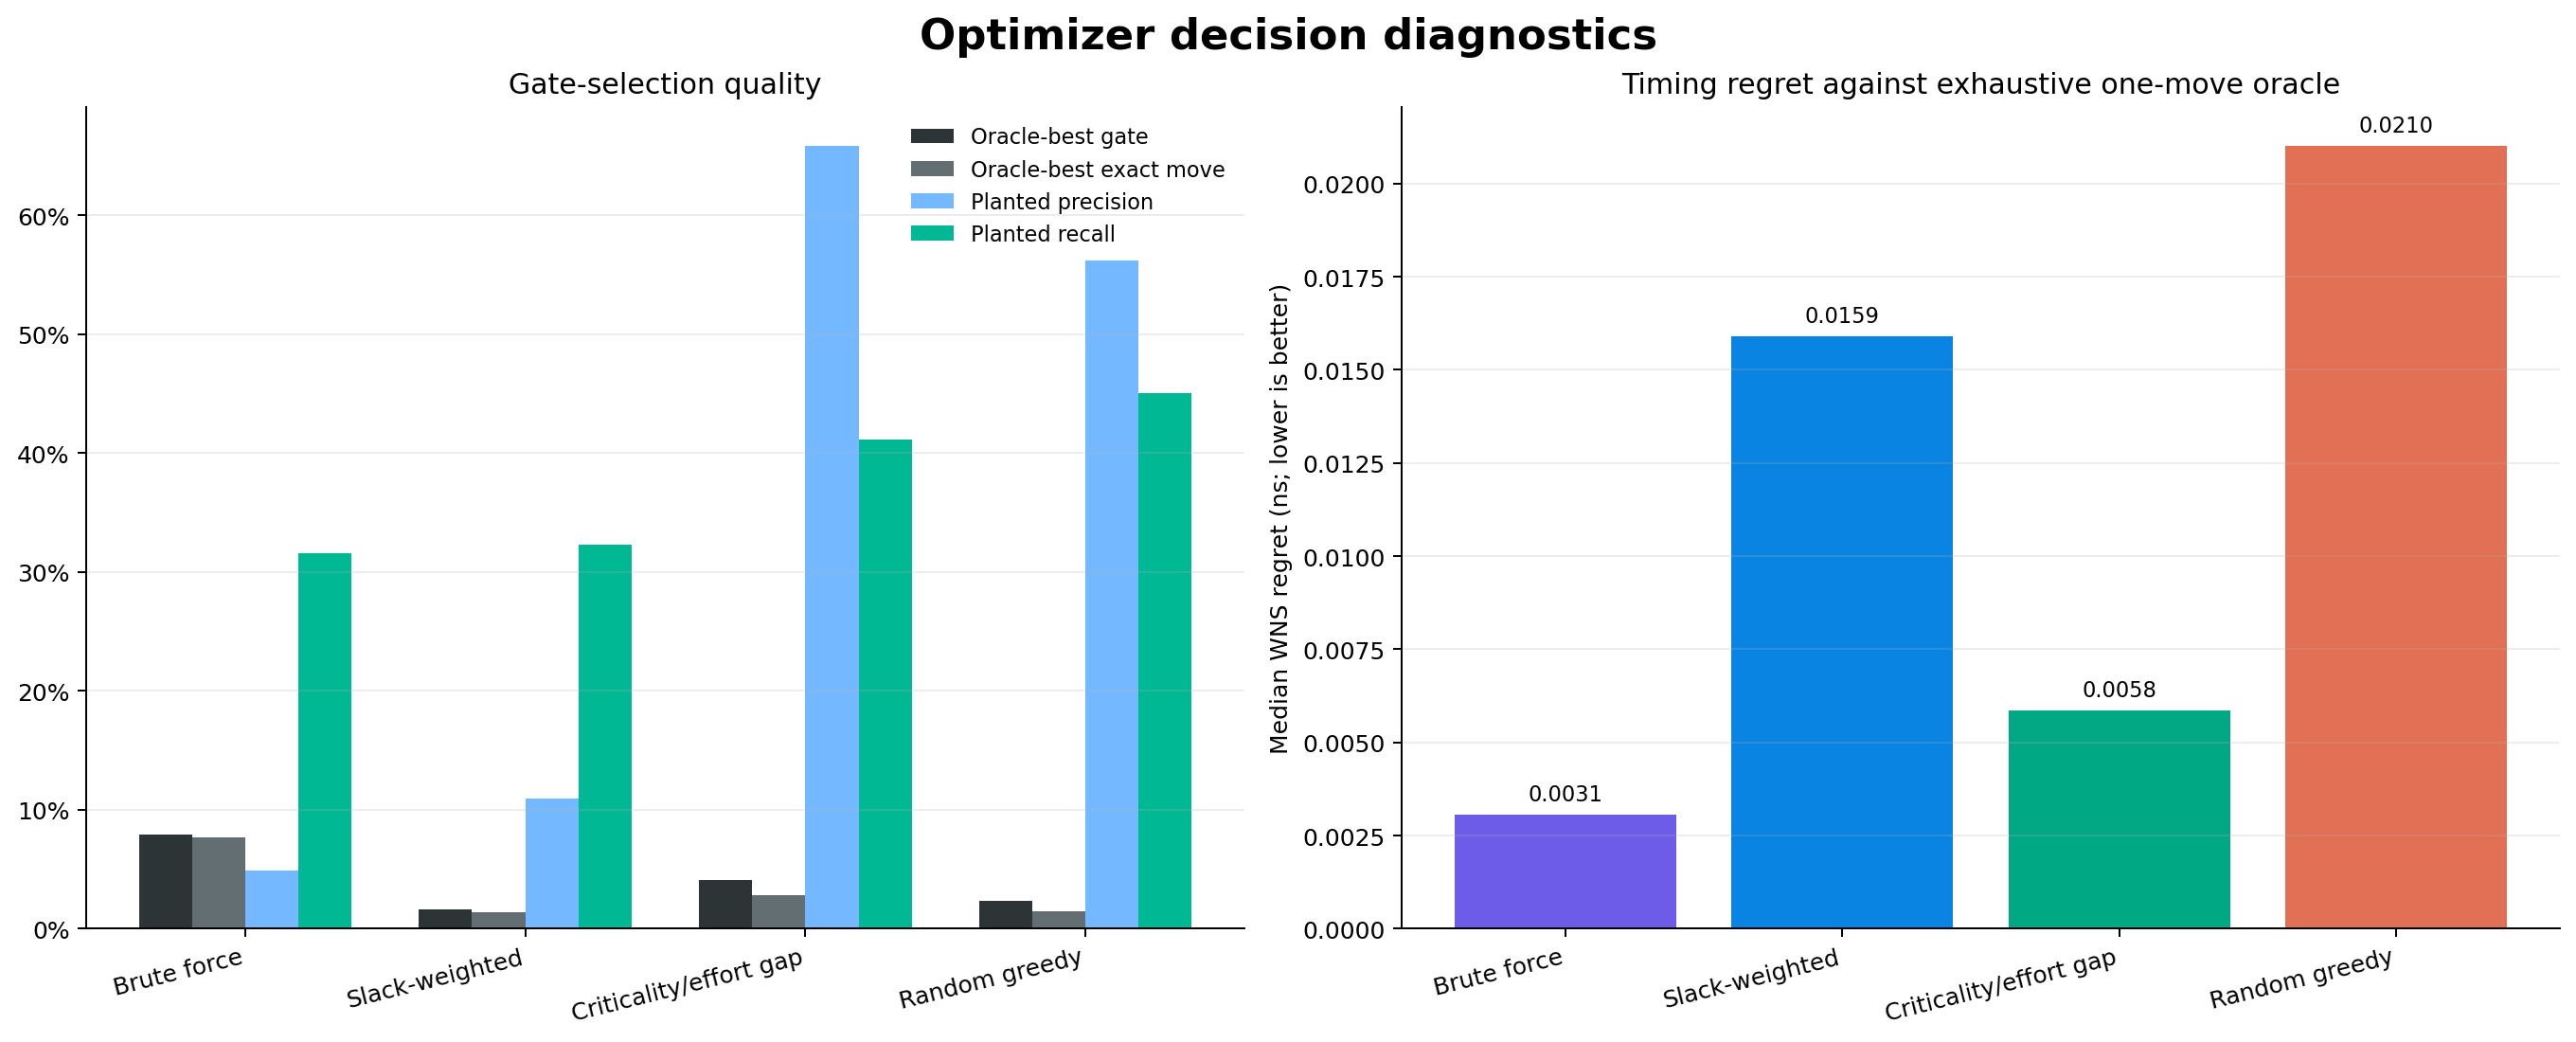
\includegraphics[width=\textwidth]{benchmarking/selection_quality.png}
    \caption{Left: gate-selection quality against the oracle's single best
    gate/exact move, and precision/recall of each heuristic's changed
    gates against the originally planted downsizing mutations. Right:
    median WNS regret against the exhaustive one-move oracle.}
    \label{fig:bench-selection-quality}
\end{figure}
 
The gate- and exact-move hit rates are low in absolute terms for
\emph{every} heuristic, including brute force ($7.9\%$/$7.7\%$) --- this
is expected, not a sign of a broken oracle: the oracle's ``best gate'' is
computed over \emph{every} legal same-family replacement on \emph{every}
gate in the circuit (\cref{sec:bench-oracle}), while even brute force only
proposes candidates on gates lying on a currently-reported critical path,
within a logical-effort-derived capacitance bracket
(\cref{sec:opt-bruteforce}); a circuit this large routinely has several
gates capable of producing an equally-good or negligibly-worse timing
improvement, so an exact match to the oracle's single top pick is a strict
criterion. The more informative signal is the \emph{median regret} column:
brute force's median regret (0.0031~ns) is roughly half of
criticality effort gap's (0.0058~ns), which is in turn roughly a third of
slack-weighted capacitance's (0.0159~ns) and random greedy's (0.0210~ns)
--- an ordering that does \emph{not} match the repair-rate ordering of
\cref{tab:bench-repair-rate} (where criticality effort gap tied brute force
and beat slack-weighted capacitance). Repair rate measures whether a
heuristic \emph{eventually} reaches compliance at all; median regret
measures how close to optimal its individual decisions are along the way.
The two metrics are related but distinct, and a heuristic can rank well on
one without ranking identically on the other.
 
The precision/recall of each heuristic's changed gates against the
\emph{originally planted} mutated gates (\cref{sec:bench-planted}) shows a
striking, and initially counter-intuitive, pattern: criticality effort gap
and random greedy --- the two \emph{weaker} heuristics by repair rate and
regret --- have substantially \emph{higher} planted-gate precision
($65.8\%$ and $56.2\%$) than brute force and slack-weighted capacitance
($4.9\%$ and $10.9\%$), whose repairs touch the originally-mutated gates
only rarely. This is consistent with, not contradictory to, the framework's
own design rationale (\cref{sec:bench-oracle}): a compliant, budget-respecting
repair is very rarely unique, and a search that draws from a wider
candidate bracket (brute force, slack-weighted capacitance) is more likely
to find an equally valid fix at a \emph{different} gate than the one
originally downsized, while a search restricted to smaller, one-step-up
moves (criticality effort gap, random greedy) is more likely to end up
reversing something closer to the original mutation simply because fewer
alternative routes are available to it. This is precisely why
\cref{ch:benchmarking} treats exact recovery of the planted mutation as a
secondary diagnostic rather than the primary correctness signal: by that
narrower measure alone, the two least effective heuristics on this suite
would appear the most accurate.
 
Finally, \emph{beats reference cost} shows a clean split along the same
line: brute force and slack-weighted capacitance --- both drawing from the
full logical-effort capacitance bracket, the same candidate source
available to the beam-search reference itself (\cref{sec:bench-reference})
--- match or beat the reference's own final cost on \emph{every}
successful repair (100.0\%), while criticality effort gap and random
greedy, restricted to one-step-up moves, fall short of it on $15\%$ and
$31\%$ of their successful repairs respectively.
 
\subsection{Convergence and Runtime Scaling}
\label{sec:res-bench-convergence}
 
\begin{figure}[H]
    \centering
    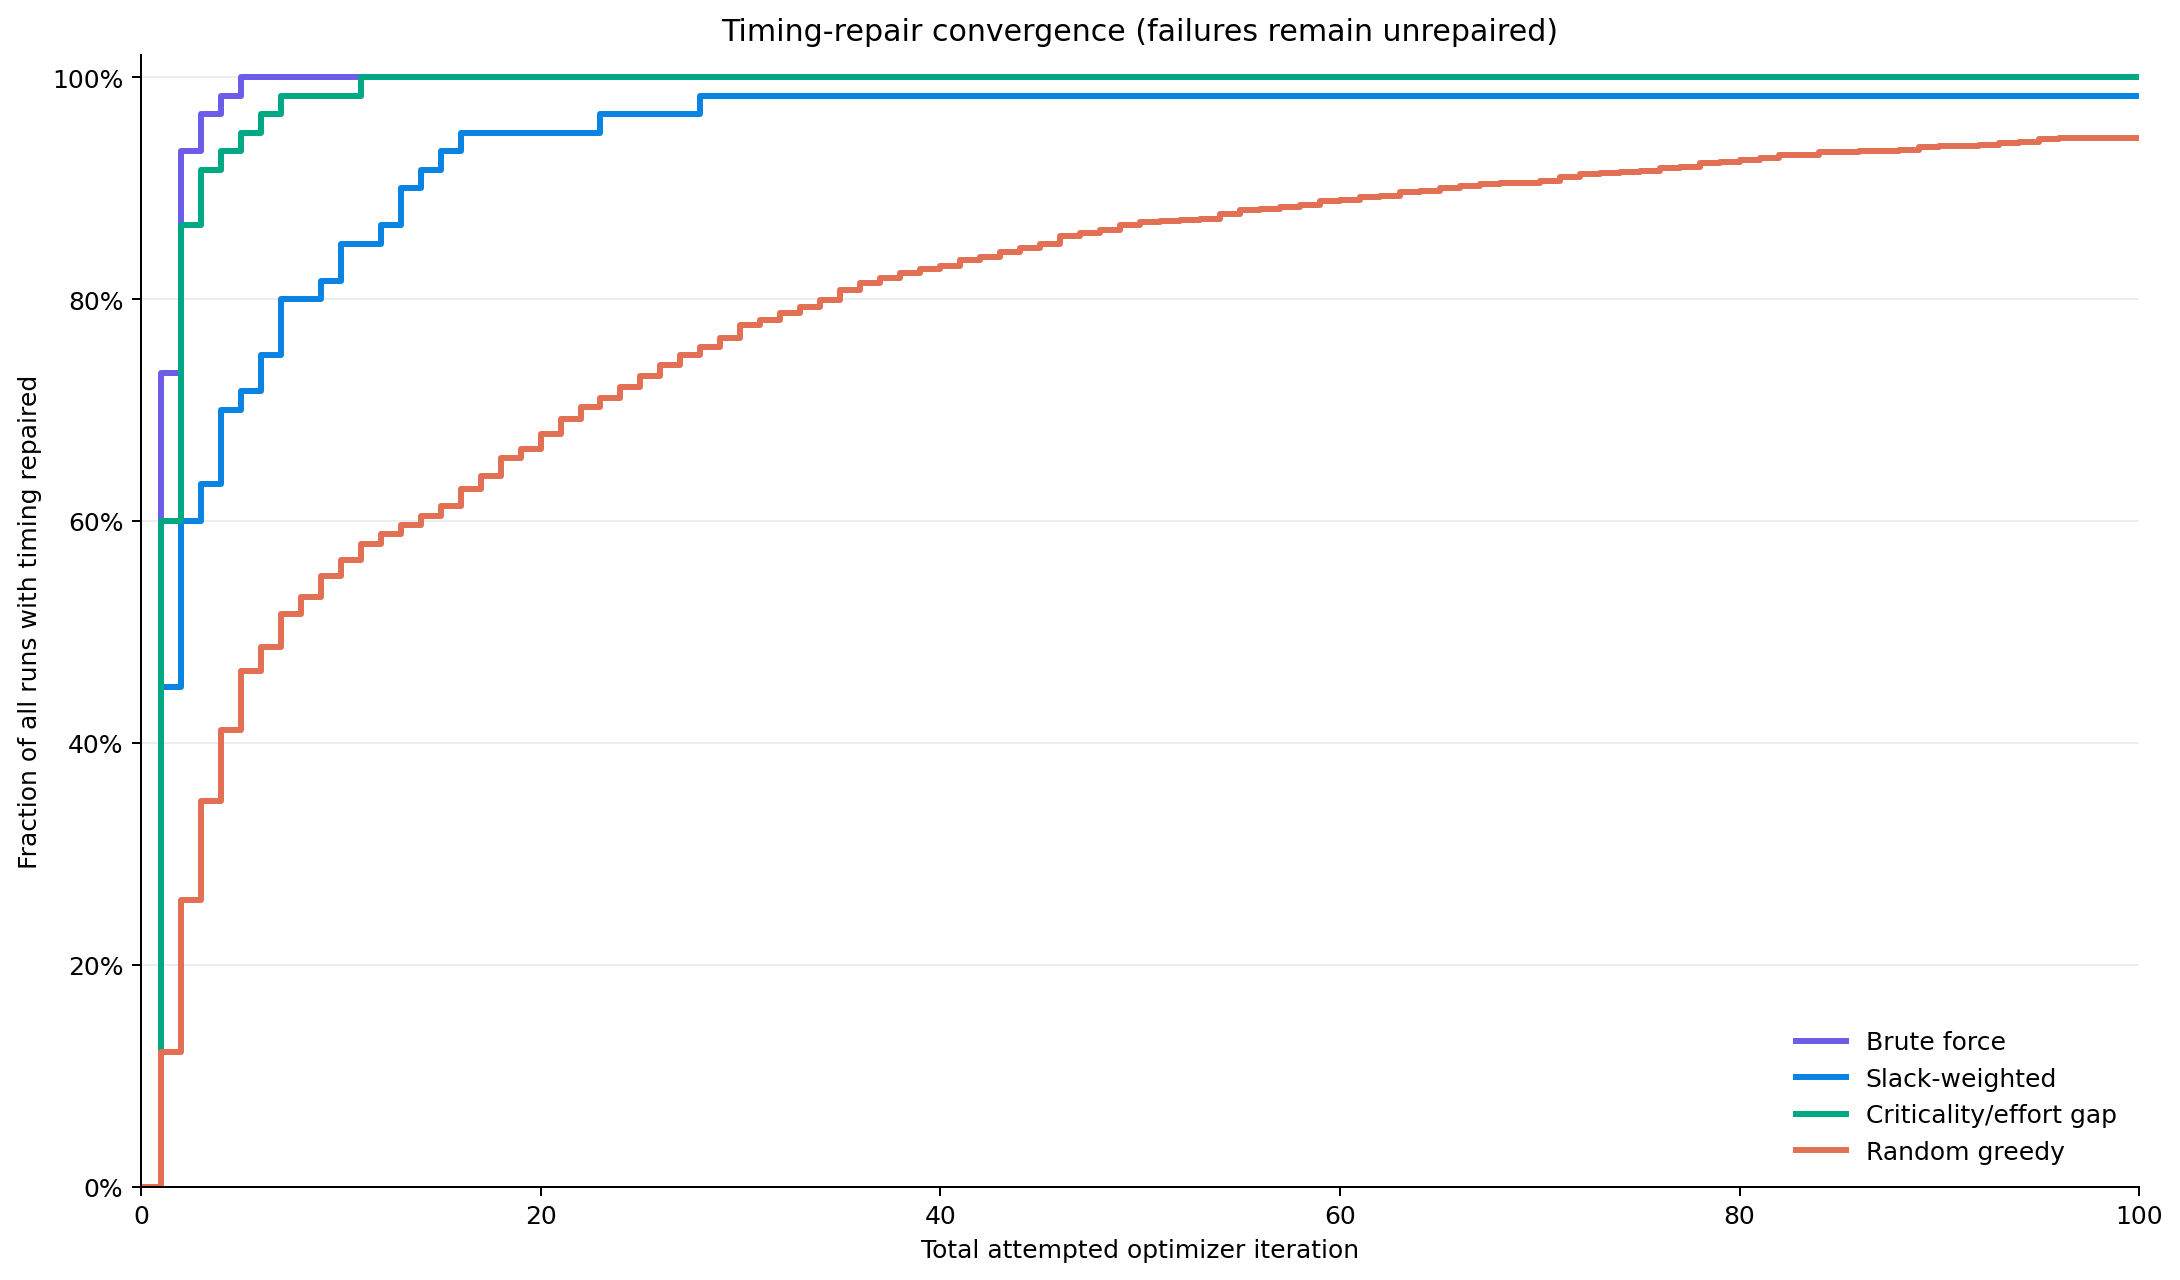
\includegraphics[width=\textwidth]{benchmarking/repair_convergence.png}
    \caption{Fraction of all 1380 runs with timing repaired, as a function
    of total attempted optimizer iterations (accepted and rejected
    attempts combined). Runs that never repair remain flat at their final
    value indefinitely.}
    \label{fig:bench-repair-convergence}
\end{figure}
 
\Cref{fig:bench-repair-convergence} shows the same repair-rate story as
\cref{tab:bench-repair-rate} unfolding over search effort rather than as a
single endpoint number: criticality effort gap and brute force both reach
their full $100\%$ repair rate within about 10 iterations, slack-weighted
capacitance climbs more gradually and plateaus just under $99\%$, and
random greedy's much shallower climb --- still visibly rising at 100
iterations --- reflects the combined effect of its unranked candidate
order (\cref{sec:opt-random-greedy}) and the cases it never resolves at
all within any of its repetitions.

\begin{figure}[H]
    \centering
    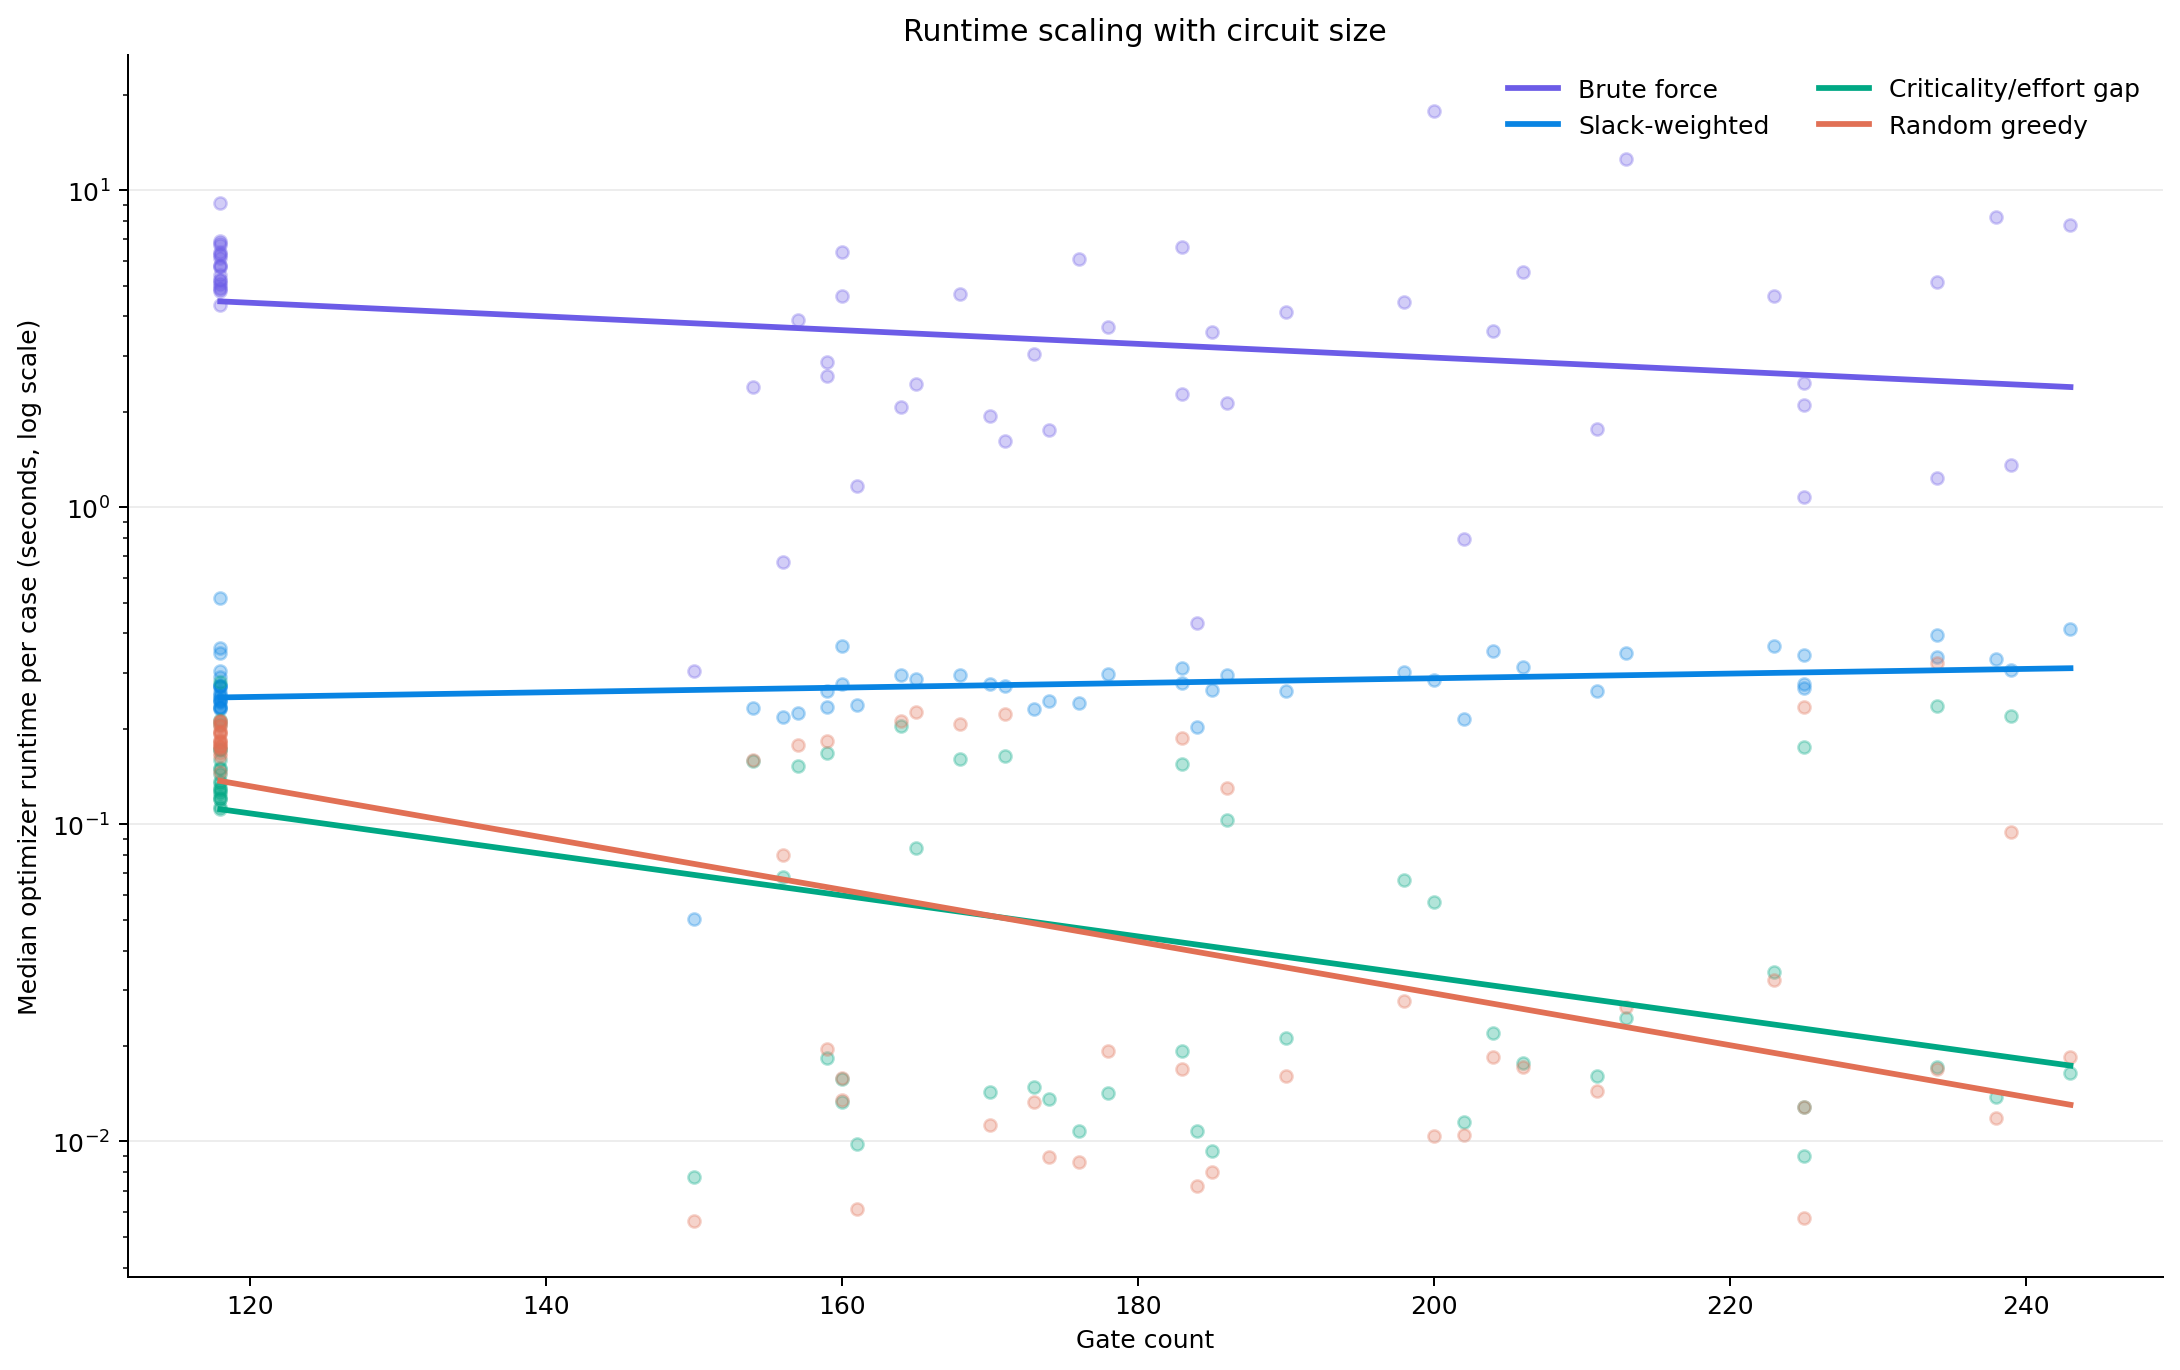
\includegraphics[width=\textwidth]{benchmarking/runtime_scalability.png}
    \caption{Median optimizer runtime per case versus gate count (log
    scale), with a fitted trend line per heuristic.}
    \label{fig:bench-runtime-scalability}
\end{figure}
 
Runtime separates the four heuristics by roughly an order of magnitude at
each tier (\cref{fig:bench-heuristic-overview}, top right; mean and
standard deviation in \cref{tab:bench-runtime}): brute force averages
$4.48\pm2.96$~s per run; slack-weighted capacitance, $0.281\pm0.063$~s;
random greedy, $0.114\pm0.099$~s; and criticality effort gap, the fastest,
$0.093\pm0.076$~s. \Cref{fig:bench-runtime-scalability} shows brute
force's runtime is roughly flat with circuit size over this suite's
150--250 gate range (its cost is dominated by the size of the candidate
bracket it evaluates per iteration, not raw gate count), while the three
sequential heuristics' runtimes visibly \emph{decrease} with gate count ---
counter-intuitive at first glance, but consistent with the suite's
generation process: larger generated circuits in this suite do not
necessarily have proportionally more or deeper critical-path violations to
repair, so the number of accepted-plus-rejected attempts needed does not
scale directly with gate count either.
 
\begin{table}[H]
\centering
\small
\begin{tabular}{@{}lrrrr@{}}
\toprule
\textbf{Heuristic} & \textbf{Mean runtime (s)} & \textbf{Std.\ dev.\ (s)} & \textbf{Mean STA calls} & \textbf{Mean final cost} \\
\midrule
BF & 4.479 & 2.962 & 1835.3 & 1.291 \\
SWC & 0.281 & 0.063 & 98.6 & 1.329 \\
RG & 0.114 & 0.099 & 51.7 & 1.369 \\
CEG & 0.093 & 0.076 & 37.0 & 1.356 \\
\bottomrule
\end{tabular}
\caption{Runtime, search cost, and mean final cost among repaired cases. BF = brute force, CEG = criticality effort gap,
SWC = slack-weighted capacitance, RG = random greedy.}
\label{tab:bench-runtime}
\end{table}
 
\subsection{Per-Case Reliability}
\label{sec:res-bench-case-reliability}
 
\begin{figure}[H]
    \centering
    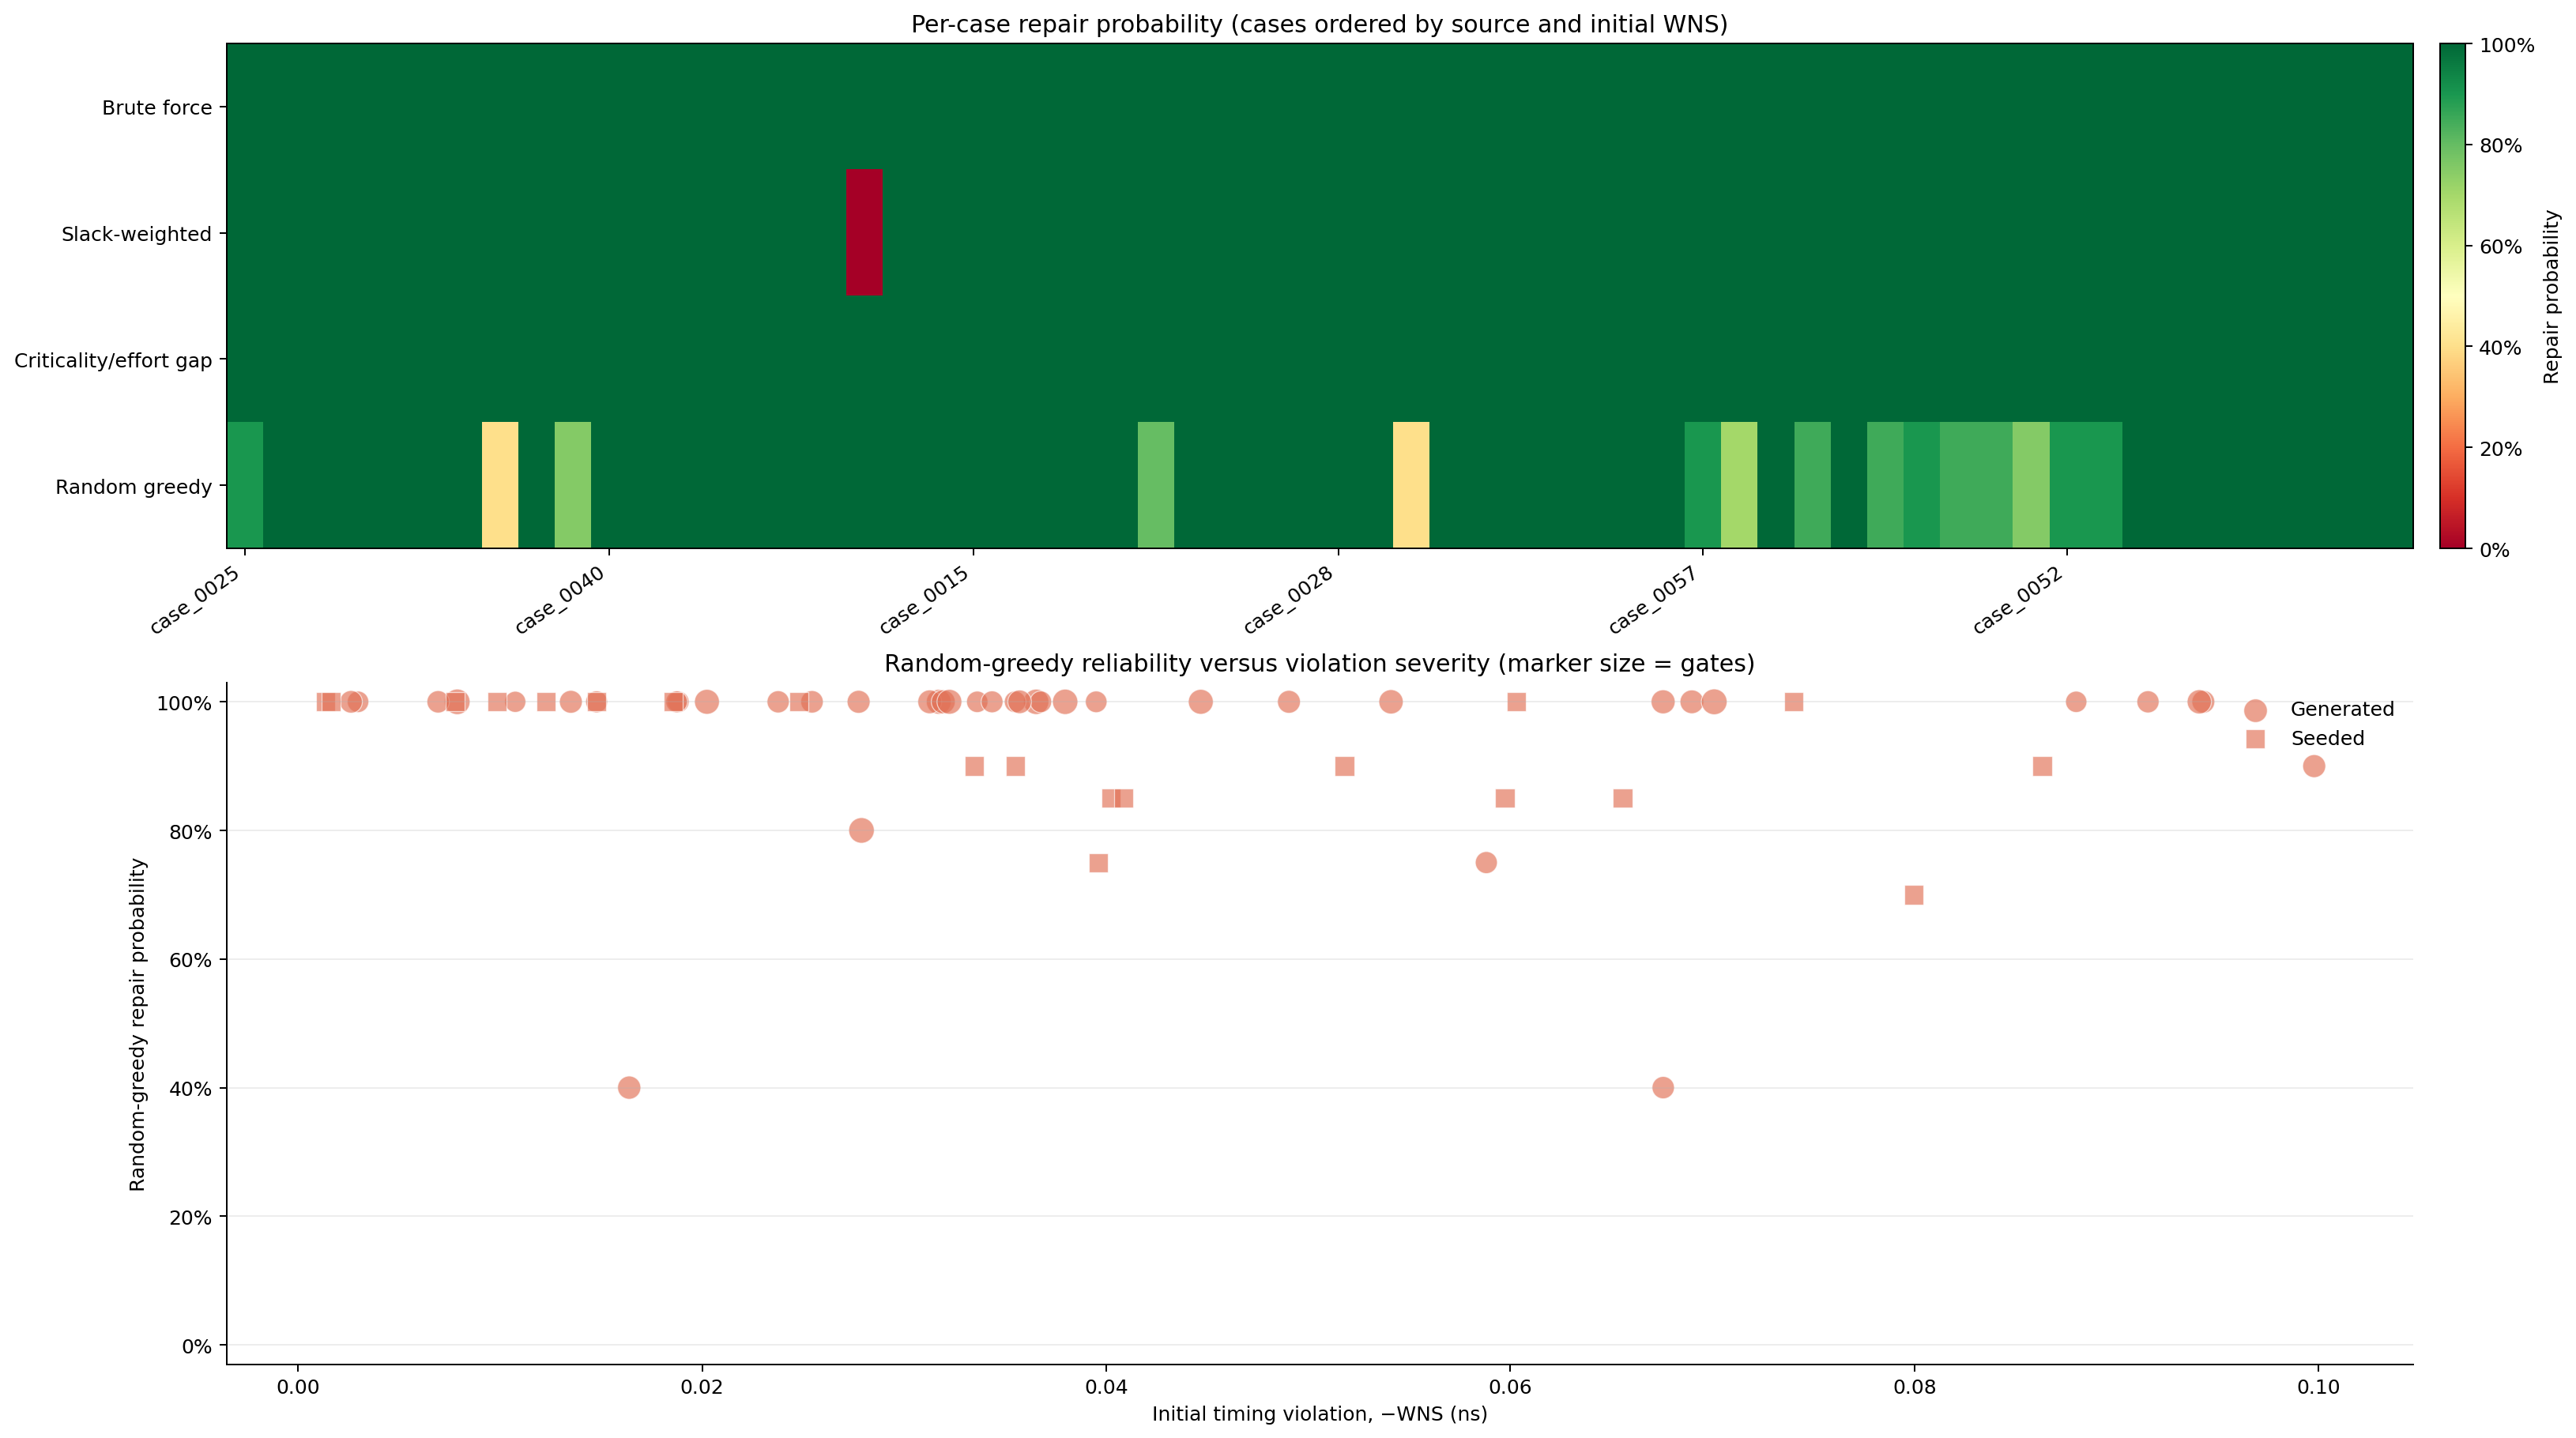
\includegraphics[width=\textwidth]{benchmarking/case_reliability.png}
    \caption{Top: per-case repair probability for a representative subset
    of cases, ordered by source and initial WNS (brute force and
    criticality effort gap are uniformly green --- always successful; the
    single dark-red cell is slack-weighted capacitance's one failure,
    \texttt{case\_0032}). Bottom: random greedy's repair probability
    (across its 20 repetitions) versus initial violation severity, marker
    size indicating gate count, split by source type.}
    \label{fig:bench-case-reliability}
\end{figure}
 
\Cref{fig:bench-case-reliability}'s lower panel makes the population-level
pattern underlying \cref{sec:res-bench-strata}'s severity stratification
directly visible at the case level: random greedy's repair probability is
$100\%$ for the great majority of cases regardless of source, but drops
into the $70$--$90\%$ range for a specific subset of harder cases, with
the two clearest outliers (both at $40\%$) occurring at moderate, not
extreme, violation severity --- reinforcing that repair difficulty for a
one-step-up, unranked search depends on circuit structure as much as on
how large the initial violation is.
 
\subsection{Stratified Breakdown}
\label{sec:res-bench-strata}
 
\Cref{tab:bench-strata} breaks the repair rate down by three groupings
computed automatically by the evaluation framework
(\cref{sec:bench-metrics}): circuit depth, reconvergence level, and
initial violation severity. (This suite's cases fall into only two buckets
each for depth and reconvergence --- \emph{medium}/\emph{deep} and
\emph{medium}/\emph{high} respectively --- reflecting the generation
configuration's target ranges, \cref{sec:res-bench-generation}; no
\emph{shallow} or \emph{low-reconvergence} cases were generated in this
run.)
 
\begin{table}[H]
\centering
\small
\begin{tabular}{@{}llrrrrr@{}}
\toprule
\textbf{Grouping} & \textbf{Stratum} & \textbf{Cases} & \textbf{BF} & \textbf{CEG} & \textbf{SWC} & \textbf{RG} \\
\midrule
\multirow{2}{*}{Depth} & Medium & 10 & 100.0\% & 100.0\% & 100.0\% & 94.0\% \\
 & Deep & 50 & 100.0\% & 100.0\% & 98.0\% & 94.6\% \\
\multirow{2}{*}{Reconvergence} & Medium & 5 & 100.0\% & 100.0\% & 100.0\% & 100.0\% \\
 & High & 55 & 100.0\% & 100.0\% & 98.2\% & 94.0\% \\
\multirow{3}{*}{Violation severity} & Mild & 8 & 100.0\% & 100.0\% & 100.0\% & 100.0\% \\
 & Moderate & 34 & 100.0\% & 100.0\% & 97.1\% & 95.4\% \\
 & Severe & 18 & 100.0\% & 100.0\% & 100.0\% & 90.3\% \\
\bottomrule
\end{tabular}
\caption{Repair rate by circuit depth, reconvergence level, and initial
violation severity. BF = brute force, CEG = criticality effort gap,
SWC = slack-weighted capacitance, RG = random greedy.}
\label{tab:bench-strata}
\end{table}
 
Brute force and criticality effort gap are unaffected by any stratum in
this suite, repairing $100\%$ of cases regardless of depth, reconvergence,
or severity. Random greedy is the only heuristic whose repair rate degrades
meaningfully with reconvergence (from $100\%$ at medium reconvergence to
$94.0\%$ at high) and with violation severity (from $100\%$ on mild
violations down to $90.3\%$ on severe ones) --- exactly where a
logical-effort-free, unranked search is least likely to stumble onto the
gate a severe or highly-reconvergent violation actually needs. Slack-weighted
capacitance shows a smaller version of the same pattern on depth
($100\%\rightarrow98.0\%$) and reconvergence ($100\%\rightarrow98.2\%$),
consistent with \code{case\_0032} --- its one failure --- being both a
deep and a reconvergent circuit. Somewhat counter-intuitively,
slack-weighted capacitance's repair rate on \emph{severe} violations
($100\%$) is \emph{higher} than on \emph{moderate} ones ($97.1\%$): the
harder-looking severity axis is not the one that predicts its failure on
this suite, depth and reconvergence are. This is exactly the kind of
heuristic-specific, non-obvious failure pattern the fixed fifteen-circuit
suite is too small to reveal, and is the clearest evidence in this report
that a large, structurally-varied synthetic suite adds information the
fixed suite alone cannot provide.


\section{Complete Per-Circuit Figures}
\label{sec:res-full-figures}

\Cref{sec:res-case-c02,sec:res-case-divergence} showed the pre-/post-
optimization circuit diagrams and convergence/outcome plots for the two
circuits most useful for illustrating \emph{why} the heuristics diverge.
The identical set of four figures --- pre-optimization diagram,
post-optimization diagram, convergence trace, and outcomes summary --- is
generated for every one of the fifteen valid benchmark circuits;
Appendix \ref{app:full-figures} reproduces the complete set for systematic
reference.

\section{Summary}
\label{sec:res-summary}

Across the fixed benchmark suite, the logical-effort-guided canonical
heuristic (slack weighted capacitance) resolved timing violations on
$13/14$ originally-violating circuits, versus $7/14$ for the
logical-effort-free random-greedy baseline, while simultaneously issuing
fewer total STA calls (119 versus 155) and reaching a strictly lower final
cost on ten of fifteen circuits (tying on the remaining five, and never
losing on any). The second logical-effort-informed
heuristic, criticality effort gap, performs comparably to the canonical
method on all but one circuit, where its different ranking signal misses a
repair that slack-weighted capacitance finds. The one Monte
Carlo-instrumented circuit shows that the nominal-case timing improvement
from optimization corresponds to a substantial real improvement in
statistical timing yield, and that the identity of the critical path itself
can shift as a result of sizing changes. These fixed-suite results are
necessarily based on a small number of circuits; \cref{sec:res-benchmarking}
reports the corresponding, statistically stronger comparison on the
synthetic benchmark suite once completed.

\input{chapters/ch13_conclusion}

\begin{appendices}

\chapter{Full Equation Reference}
\label{app:equations}

This appendix collects every governing equation used in this report, in
one place, for quick reference during the presentation.

\begin{align*}
    C_{\mathrm{load},i} &= \sum_{(j,p)\,\in\,\mathrm{Fanout}(i)} C_{\mathrm{input},j,p} + C_{\mathrm{external},i} & &\text{(\cref{eq:cload})}\\
    D_{\mathrm{rise}/\mathrm{fall},i} &= D_{\mathrm{intrinsic},\mathrm{rise}/\mathrm{fall},i} + \kappa\, R_{\mathrm{rise}/\mathrm{fall},i}\, C_{\mathrm{load},i} & &\text{(\cref{eq:drise,eq:dfall})}\\
    \mathrm{AT}_i^{s} &= \max_{p,\,j,\,(s',s)\in\mathcal{T}_{i,p}} \left(\mathrm{AT}_j^{s'} + D_i^{s}\right) & &\text{(\cref{eq:forward-sta})}\\
    \mathrm{RT}_j^{s'} &= \min_{(i,p)\in\mathrm{Fanout}(j),\,(s',s)\in\mathcal{T}_{i,p}} \left(\mathrm{RT}_i^{s} - D_i^{s}\right) & &\text{(\cref{eq:backward-sta})}\\
    S_i^{s} &= \mathrm{RT}_i^{s} - \mathrm{AT}_i^{s}, \quad S_i = \min(S_i^{\mathrm{rise}}, S_i^{\mathrm{fall}}) & &\text{(\cref{eq:slack})}\\
    \mathrm{WNS} &= \min_{o\in\mathcal{O}} S_o, \quad \mathrm{TNS} = \sum_{o\in\mathcal{O}} \min(0,S_o) & &\text{(\cref{eq:wns-tns})}\\
    b_i &= \frac{C_{\mathrm{onpath},i}+C_{\mathrm{offpath},i}}{C_{\mathrm{onpath},i}}, \quad h_i = \frac{C_{\mathrm{onpath},i}}{C_{\mathrm{in},i}}, \quad f_i = g_i b_i h_i & &\text{(\cref{eq:le-stage})}\\
    G &= \prod_i g_i, \quad B = \prod_i b_i, \quad H = \frac{C_{L,\mathrm{path}}}{C_{\mathrm{in},1}}, \quad F = GBH & &\text{(\cref{eq:le-path})}\\
    \hat f &= F^{1/N}, \quad D_{LE,\mathrm{min}} = \tau\left(NF^{1/N}+P\right) & &\text{(\cref{eq:le-min-delay})}\\
    C^{*}_{\mathrm{in},i} &= \frac{g_i C_{\mathrm{total},i}}{\hat f} & &\text{(\cref{eq:le-target-cap})}\\
    A_{\mathrm{total}} &= \sum_i A_i, \quad C_{\mathrm{sw},i} = C_{\mathrm{load},i}+C_{\mathrm{internal},i}, \quad P_{\mathrm{dynamic}} = \sum_i \alpha_i C_{\mathrm{sw},i} V_{DD}^2 f & &\text{(\cref{eq:power-area})}\\
    P_{\mathrm{total}} &= P_{\mathrm{dynamic}} + P_{\mathrm{leakage}} & &\text{(\cref{eq:power-total})}\\
    D^{(k)}_{i,s} &= D_{i,s,\mathrm{nom}}\left(1+\sigma_g Z_g^{(k)} + \sigma_l Z_i^{(k)}\right) & &\text{(\cref{eq:mc-delay})}\\
    \hat P_{\mathrm{violation}} &= \frac1M\sum_k I^{(k)}_{\mathrm{violation}}, \quad \hat Y_{\mathrm{timing}} = 1-\hat P_{\mathrm{violation}} & &\text{(\cref{eq:mc-yield})}\\
    J &= w_D\frac{D_{\mathrm{circuit}}}{D_{\mathrm{ref}}} + w_P\frac{P_{\mathrm{total}}}{P_{\mathrm{ref}}} + w_A\frac{A_{\mathrm{total}}}{A_{\mathrm{ref}}} + \lambda\frac{\max(0,-\mathrm{WNS})}{T_{\mathrm{ref}}} & &\text{(\cref{eq:cost})}
\end{align*}

\chapter{Complete Per-Circuit Figures}
\label{app:full-figures}

For every one of the fifteen valid benchmark circuits, this appendix
reproduces the pre-optimization circuit diagram, the post-optimization
circuit diagram (canonical slack-weighted-capacitance heuristic), the
convergence trace of all three sequential heuristics
(\cref{sec:opt-heuristics}), and the final outcomes summary, in that
order. \Cref{sec:res-case-c02,sec:res-case-divergence} discuss
\texttt{c02\_basic\newline \_nand\_path} and
\texttt{c13\_large\_reconvergent\_network} specifically; they are
reproduced here again for completeness alongside the rest of the suite.
The circuit-diagram renderings of the three largest circuits
(\texttt{c13}--\texttt{c15}, 74--118 gates) are included for completeness
but are more legibly explored via the interactive topology viewer
(\cref{ch:viewer}) than at the fixed page width used here.

\section{\texttt{c01\_inverter\_chain} (3 gates)}
\label{app:fig-c01-inverter-chain}

\begin{figure}[H]
    \centering
    \begin{subfigure}[t]{0.48\textwidth}
        \centering
        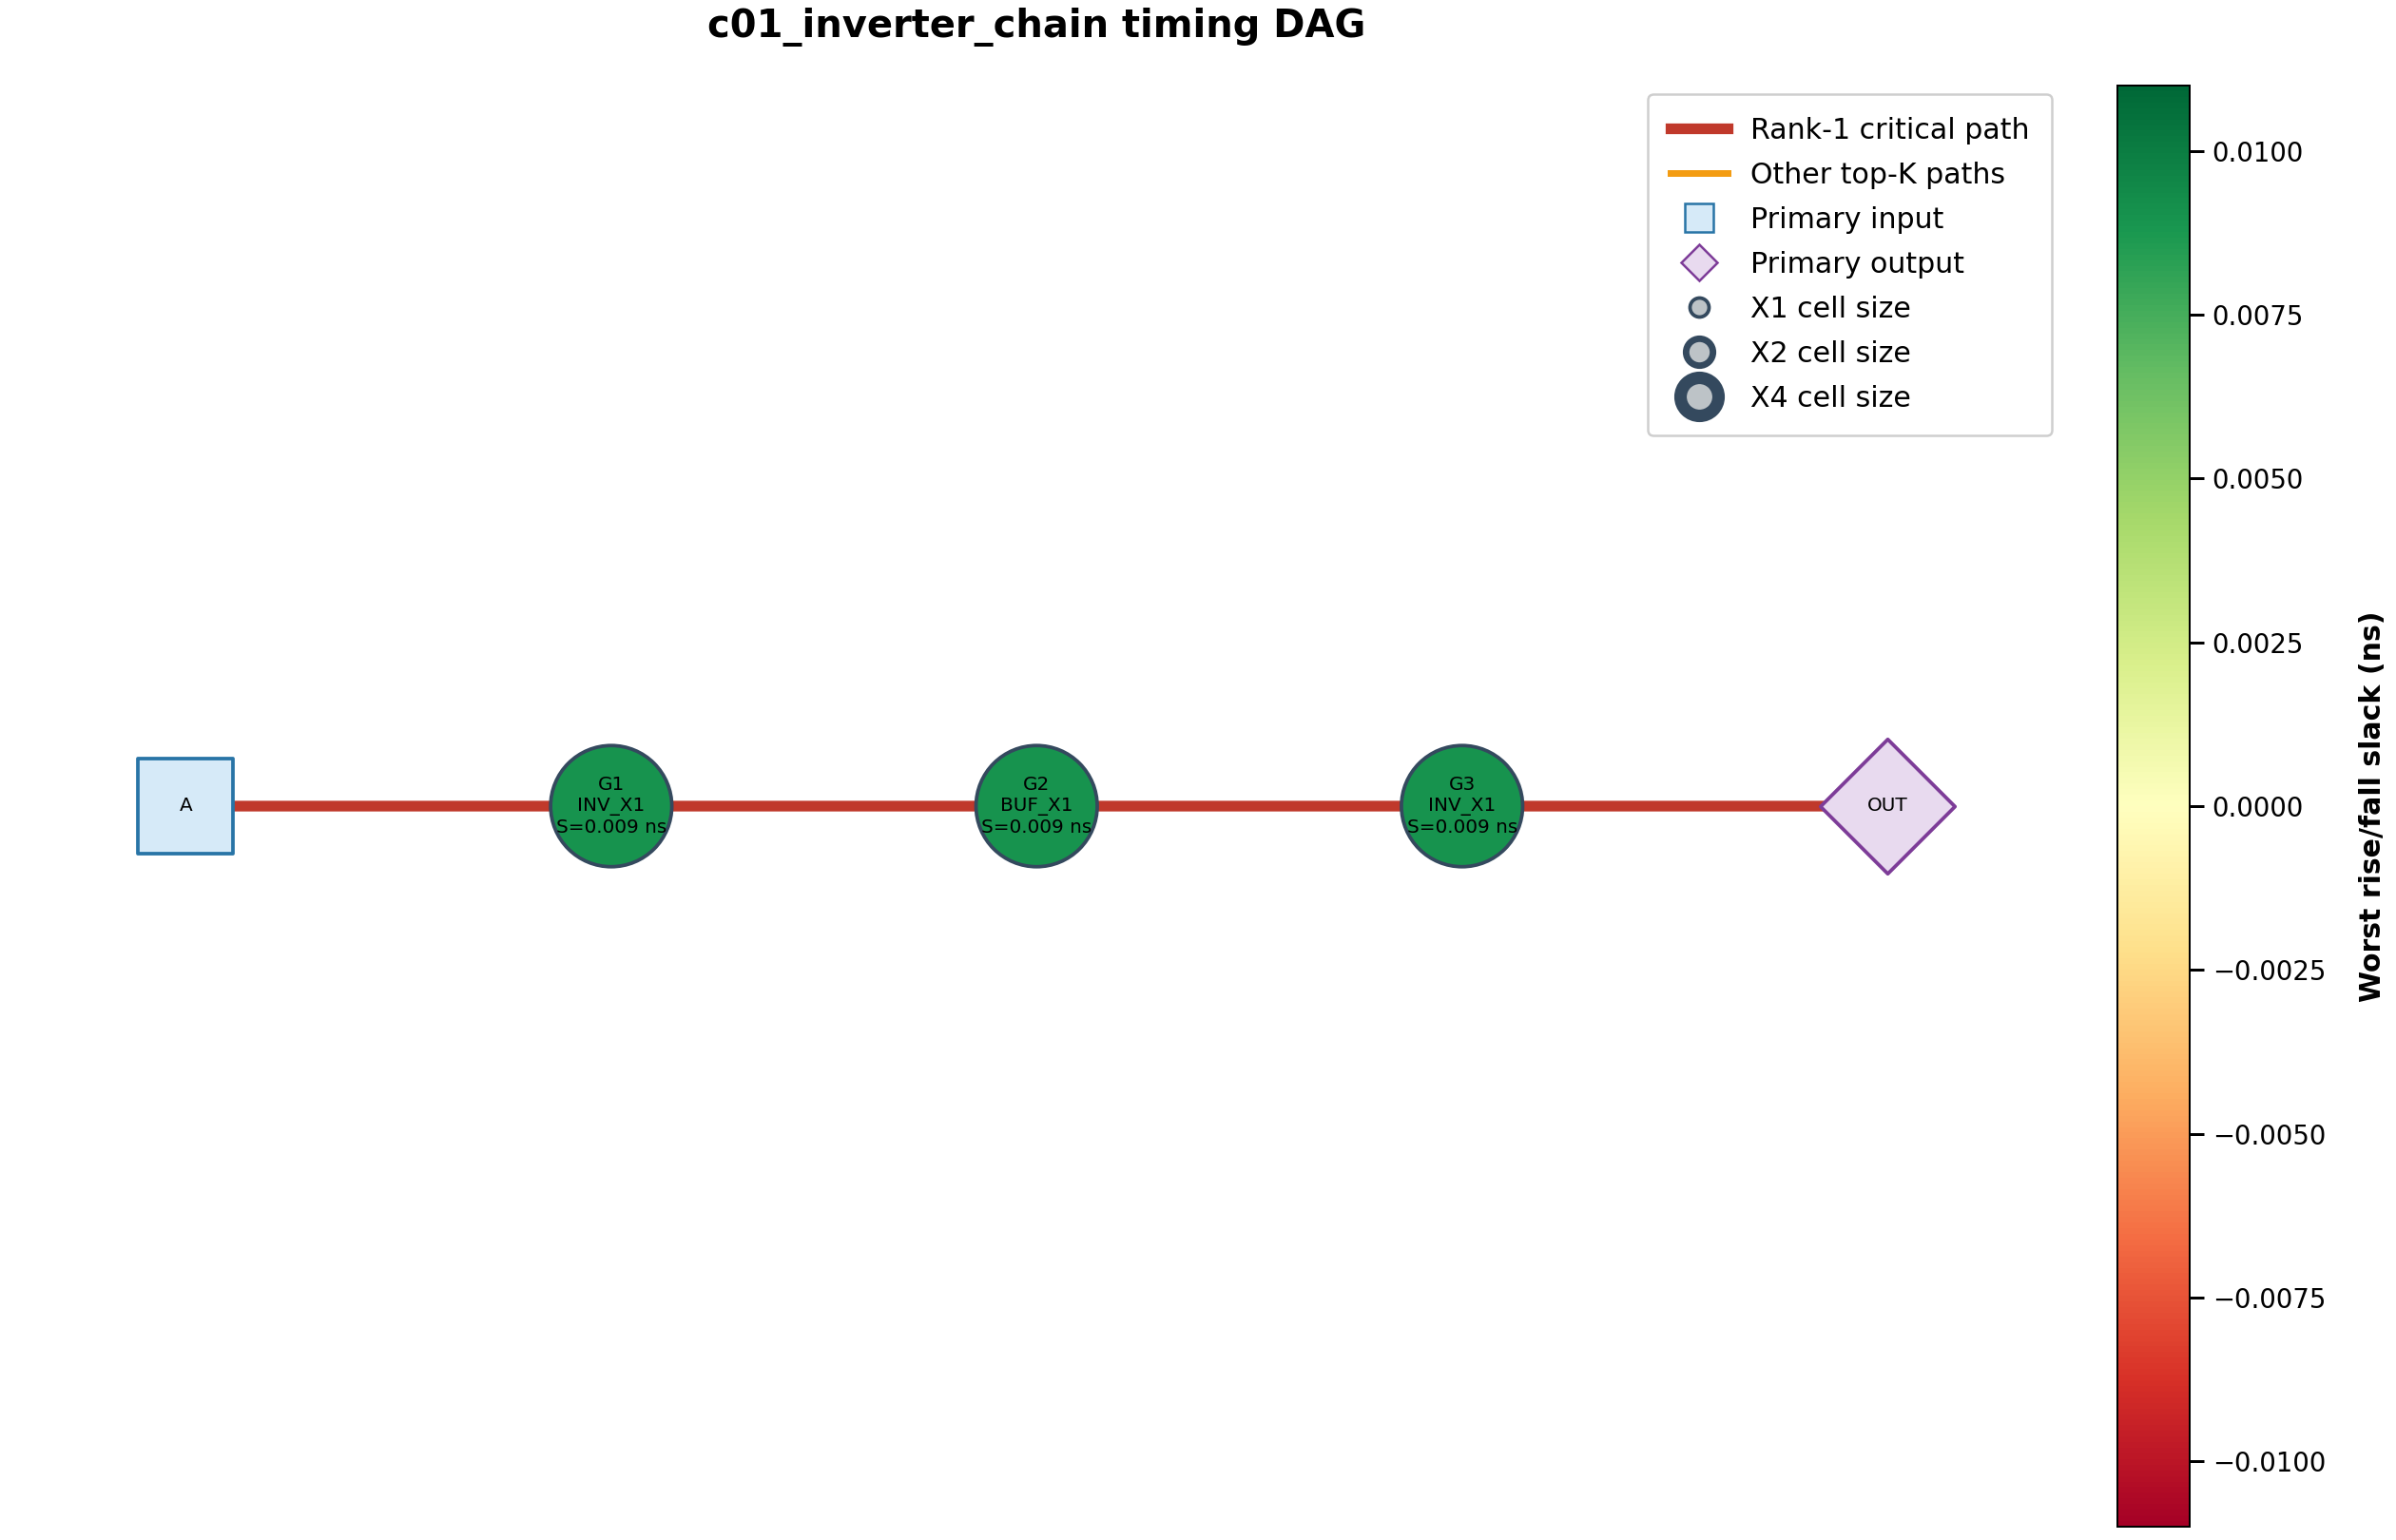
\includegraphics[width=\textwidth]{c01_inverter_chain_pre.png}
        \caption{Pre-optimization}
    \end{subfigure}
    \hfill
    \begin{subfigure}[t]{0.48\textwidth}
        \centering
        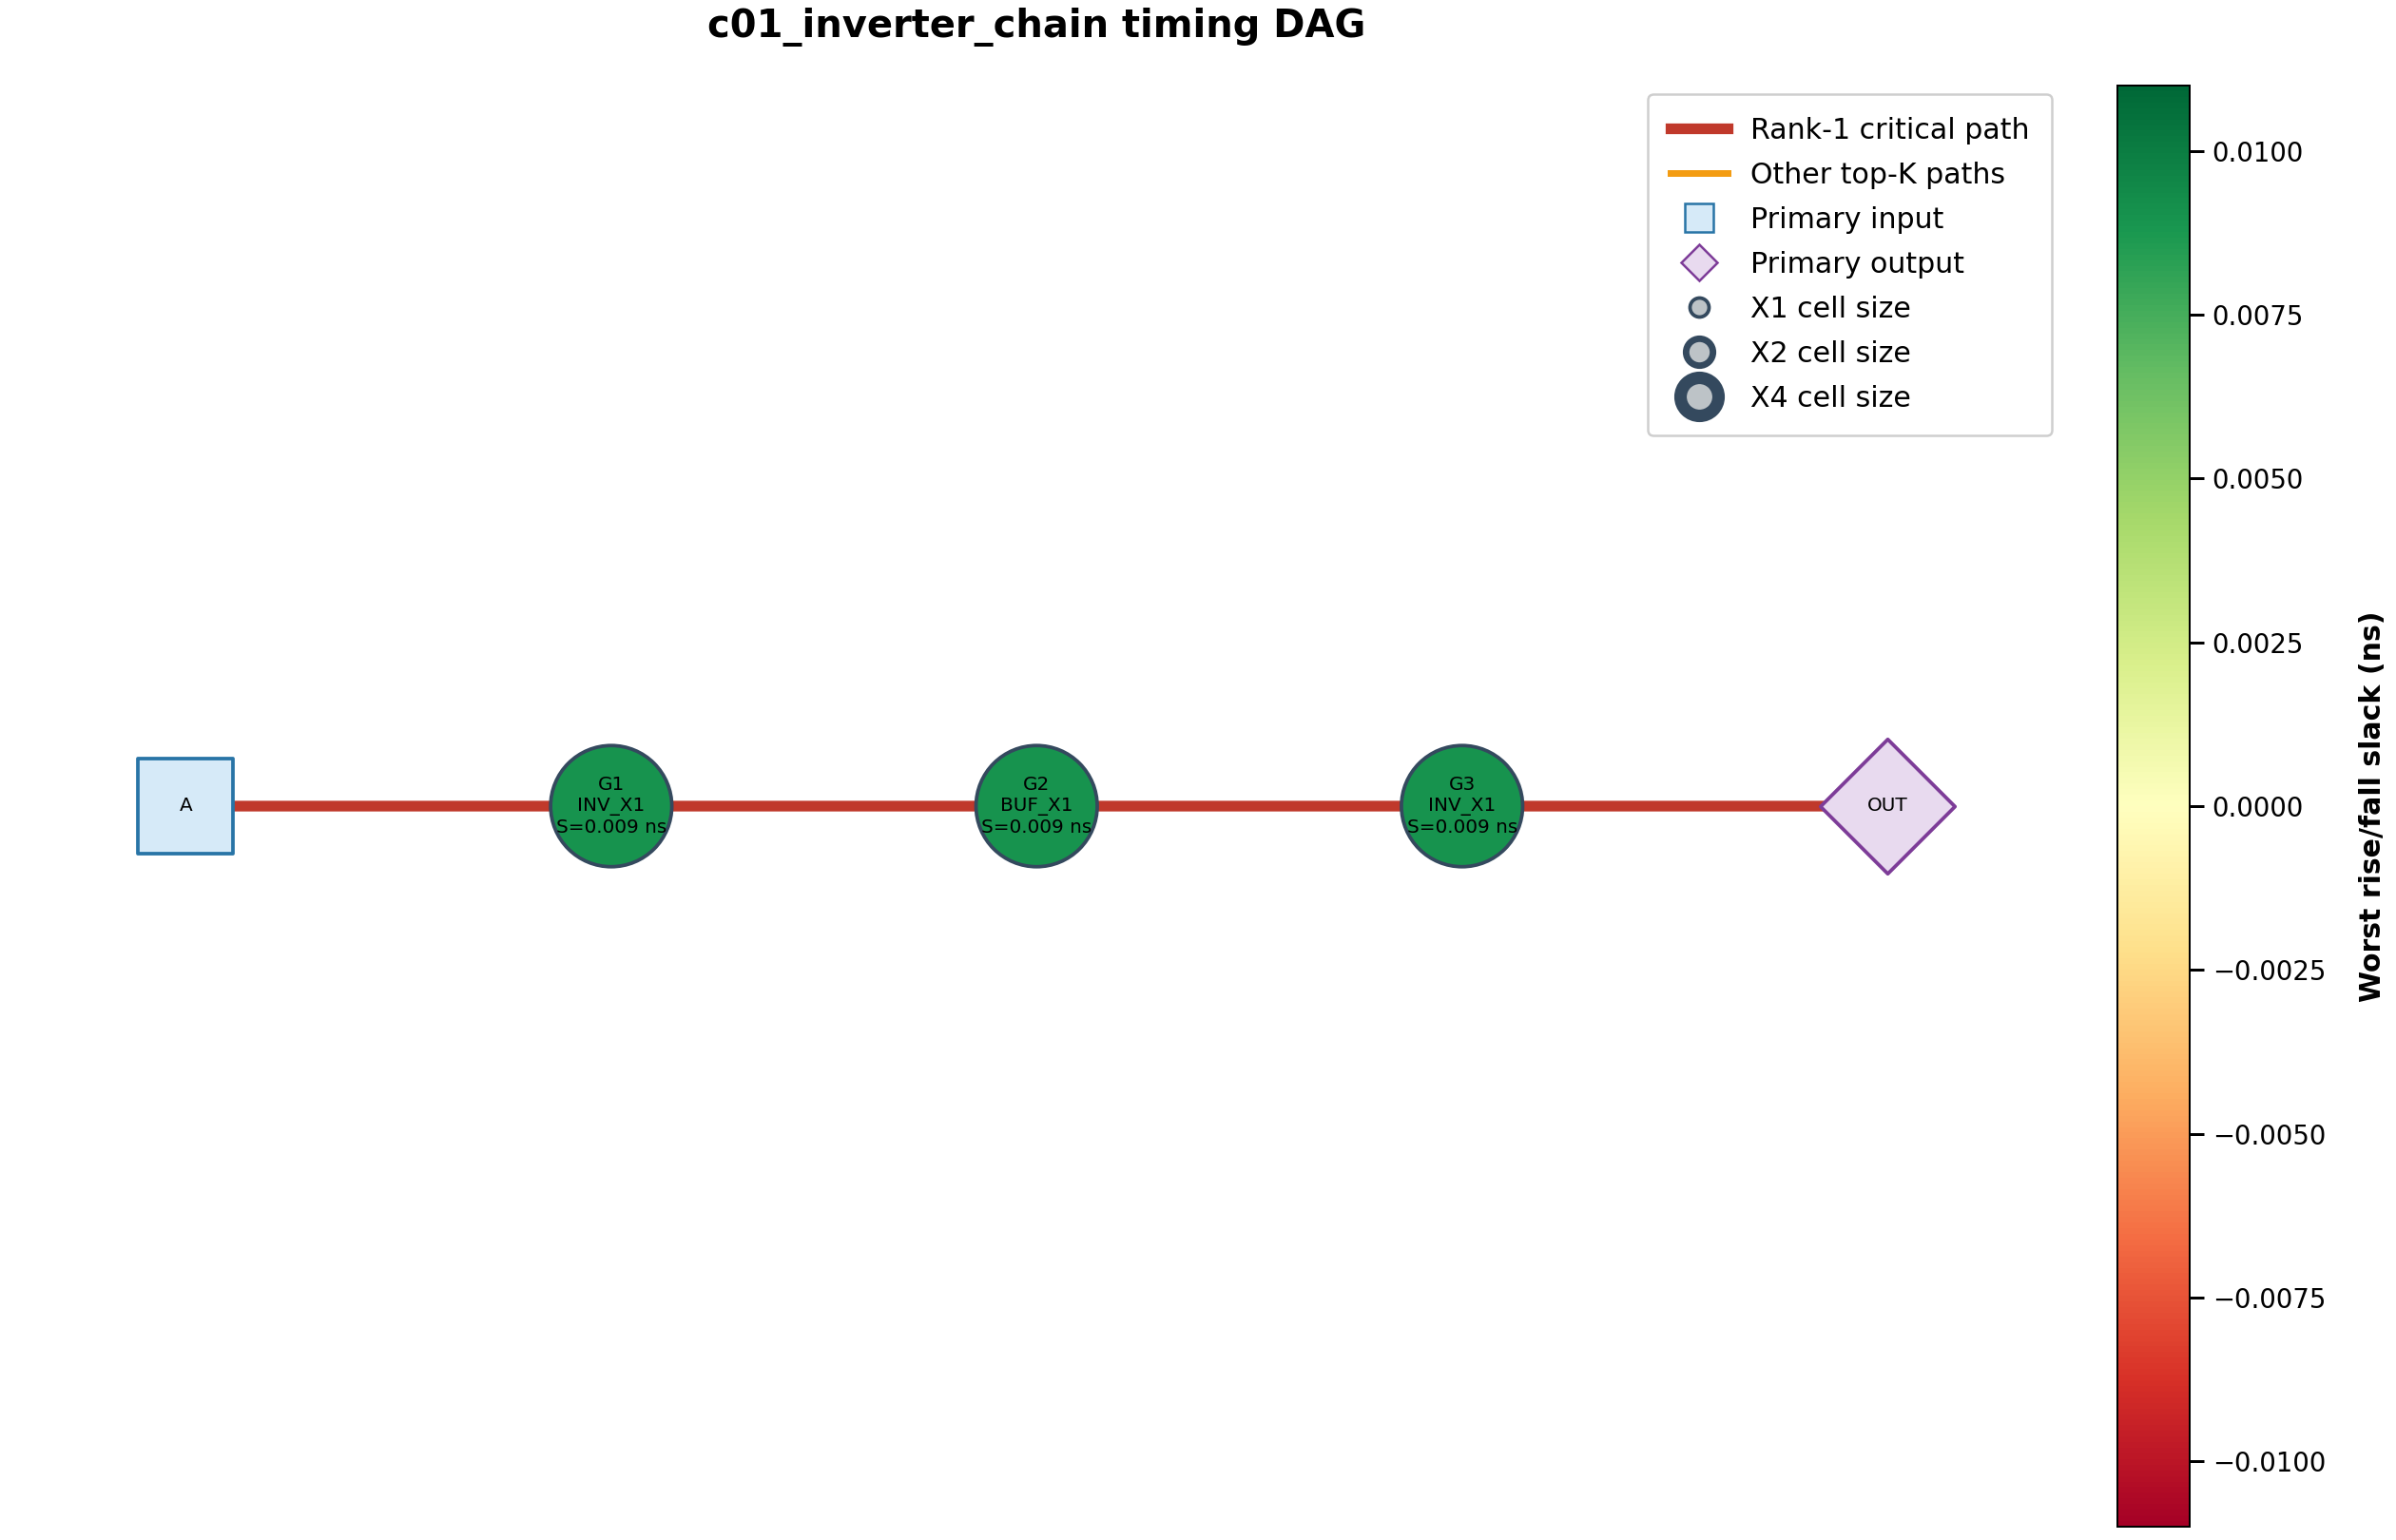
\includegraphics[width=\textwidth]{c01_inverter_chain_post.png}
        \caption{Post-optimization}
    \end{subfigure}
    \caption{\texttt{c01\_inverter\_chain}: circuit diagrams, nodes colored by slack,
    critical path highlighted.}
    \label{fig:app-c01-inverter-chain-graphs}
\end{figure}

\begin{figure}[H]
    \centering
    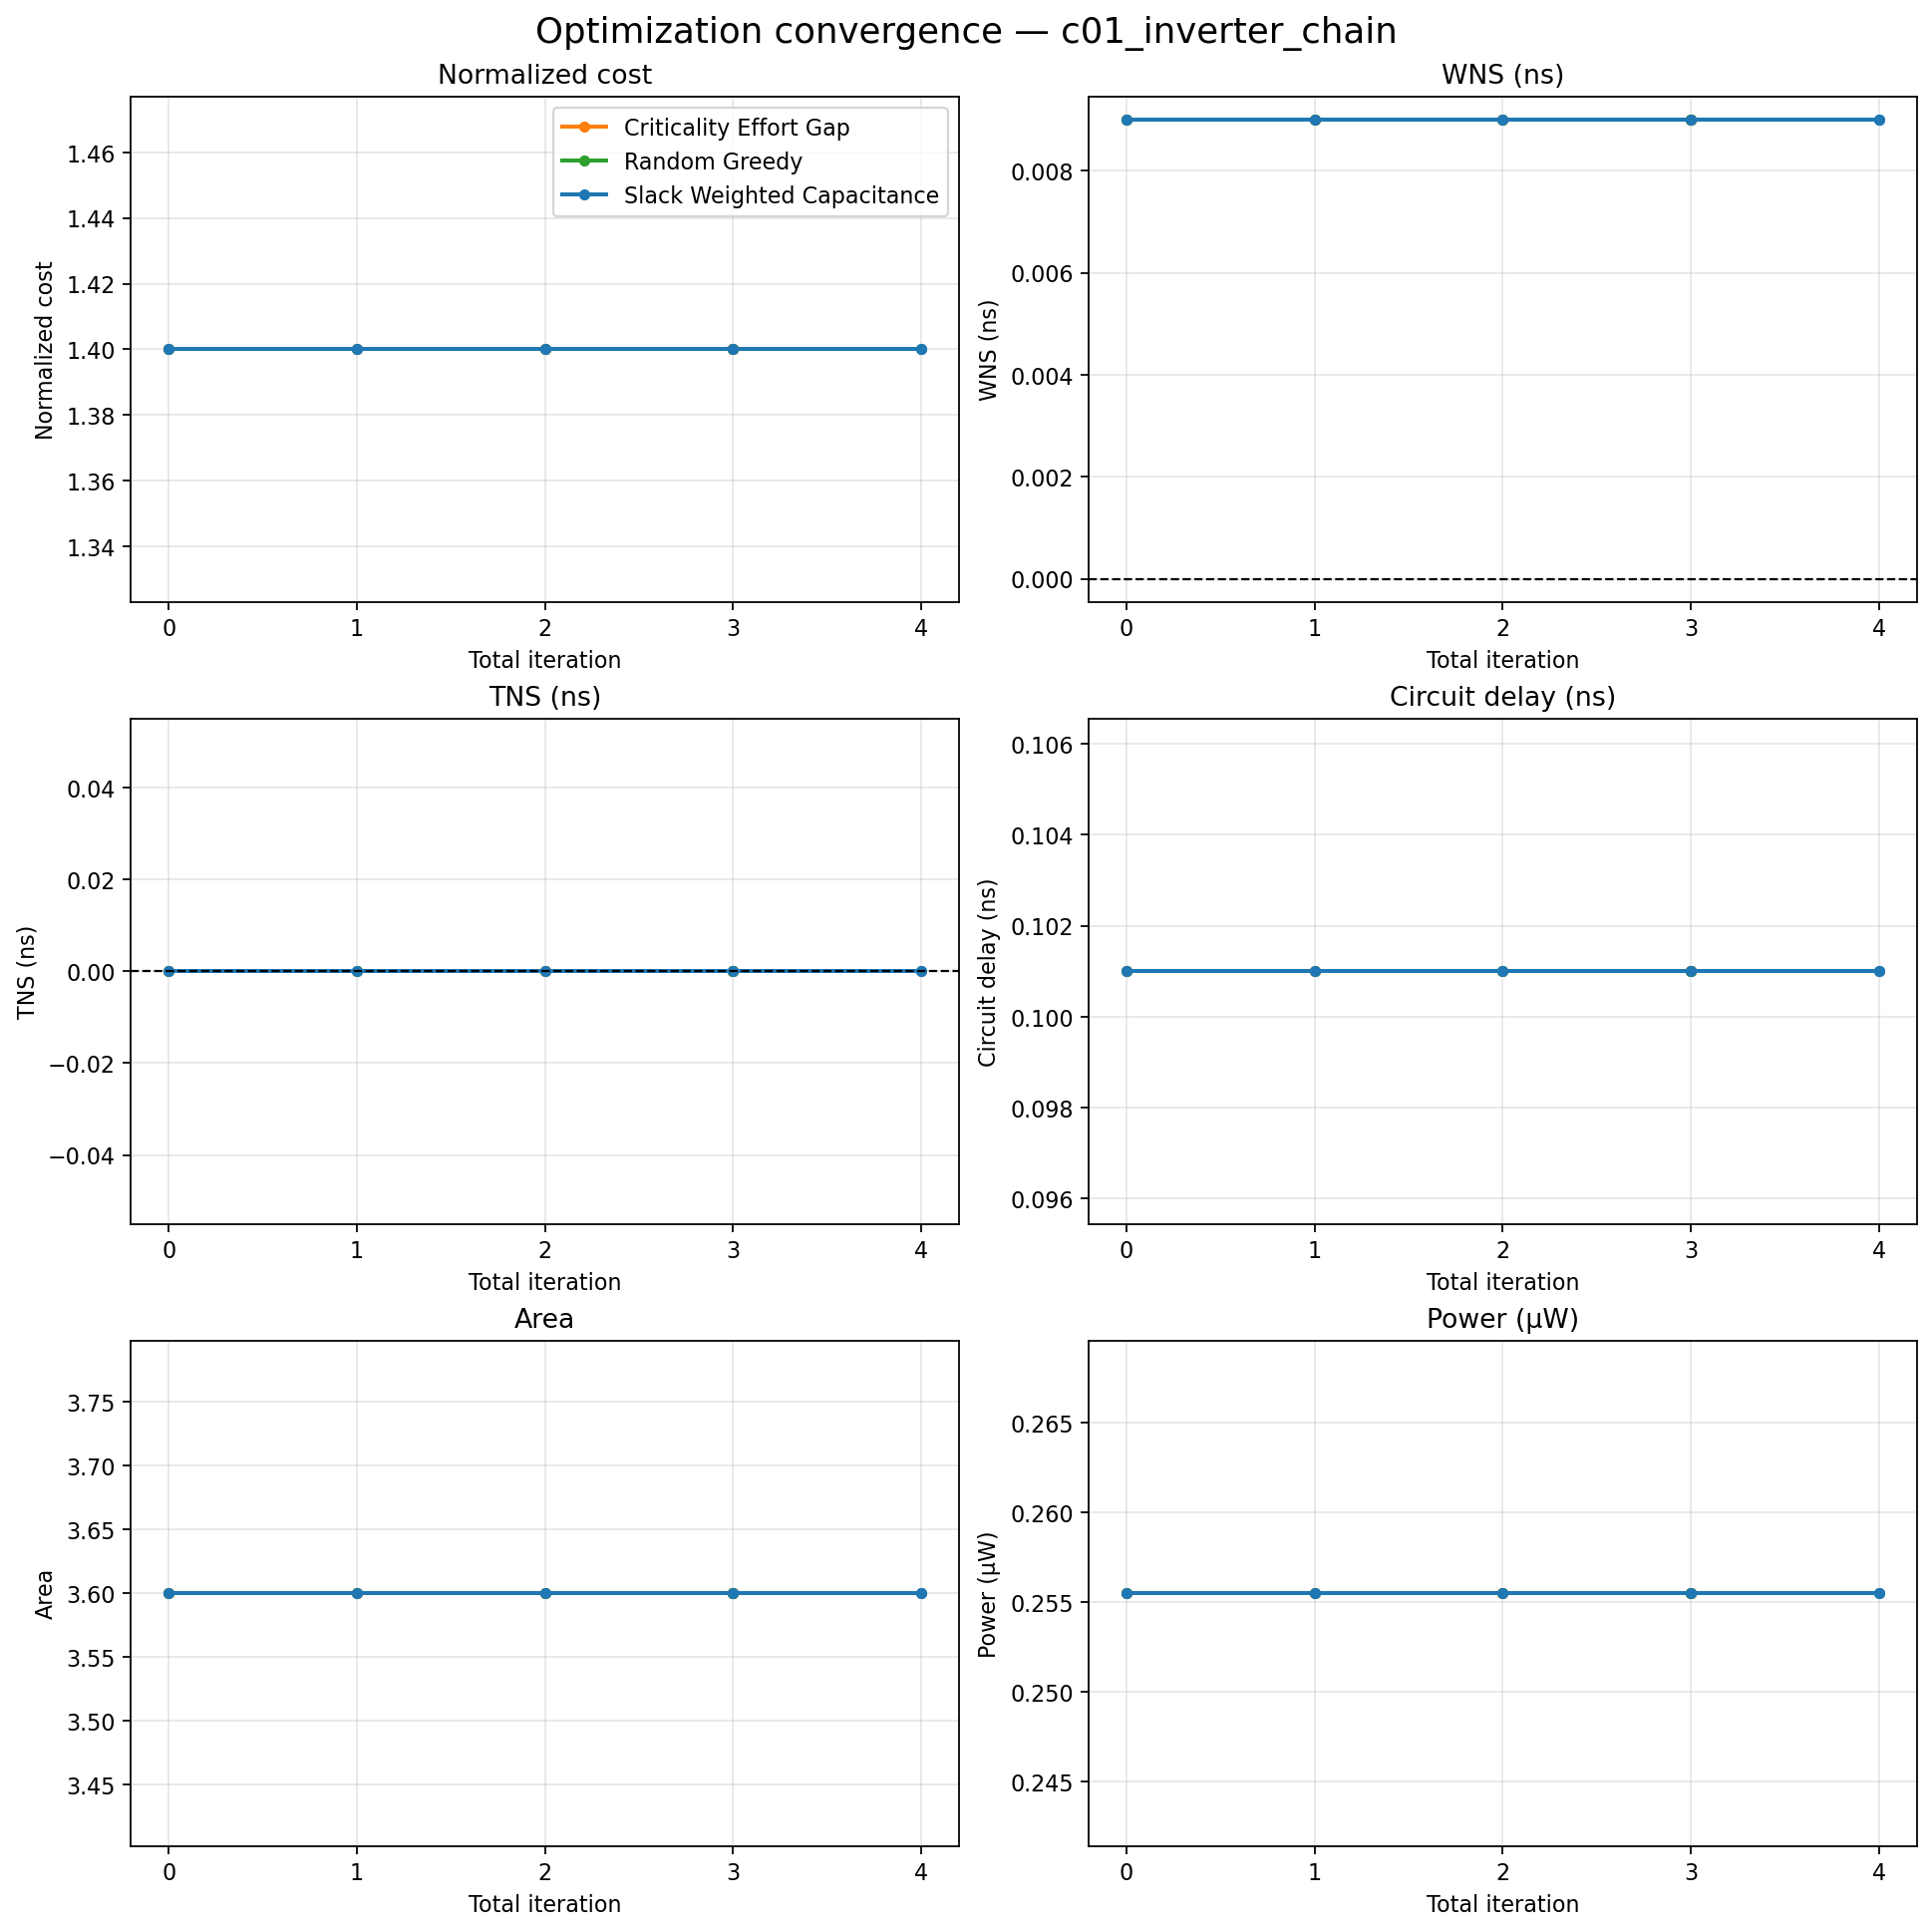
\includegraphics[width=\textwidth]{c01_inverter_chain_conv.png}
    \caption{\texttt{c01\_inverter\_chain}: optimization convergence trace.}
    \label{fig:app-c01-inverter-chain-conv}
\end{figure}

\begin{figure}[H]
    \centering
    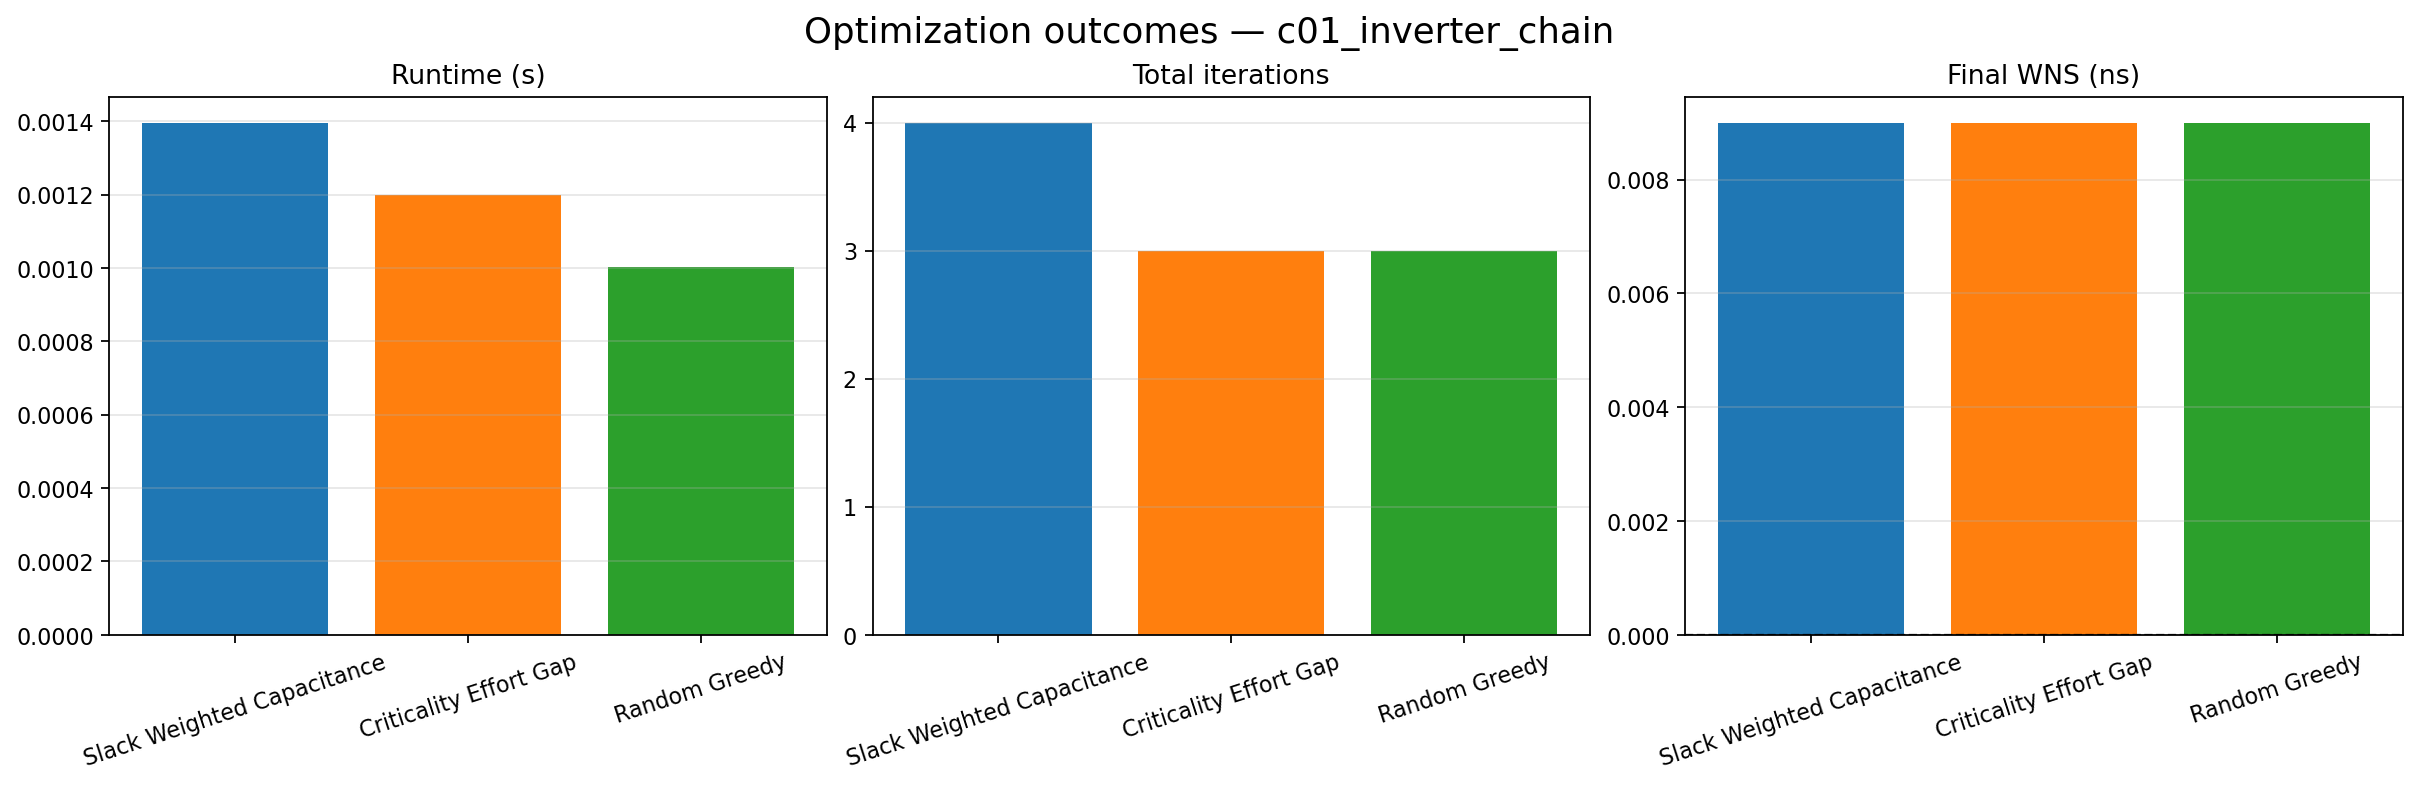
\includegraphics[width=\textwidth]{c01_inverter_chain_outc.png}
    \caption{\texttt{c01\_inverter\_chain}: optimization outcomes summary.}
    \label{fig:app-c01-inverter-chain-outc}
\end{figure}

\clearpage

\section{\texttt{c02\_basic\_nand\_path} (3 gates)}
\label{app:fig-c02-basic-nand-path}

\begin{figure}[H]
    \centering
    \begin{subfigure}[t]{0.48\textwidth}
        \centering
        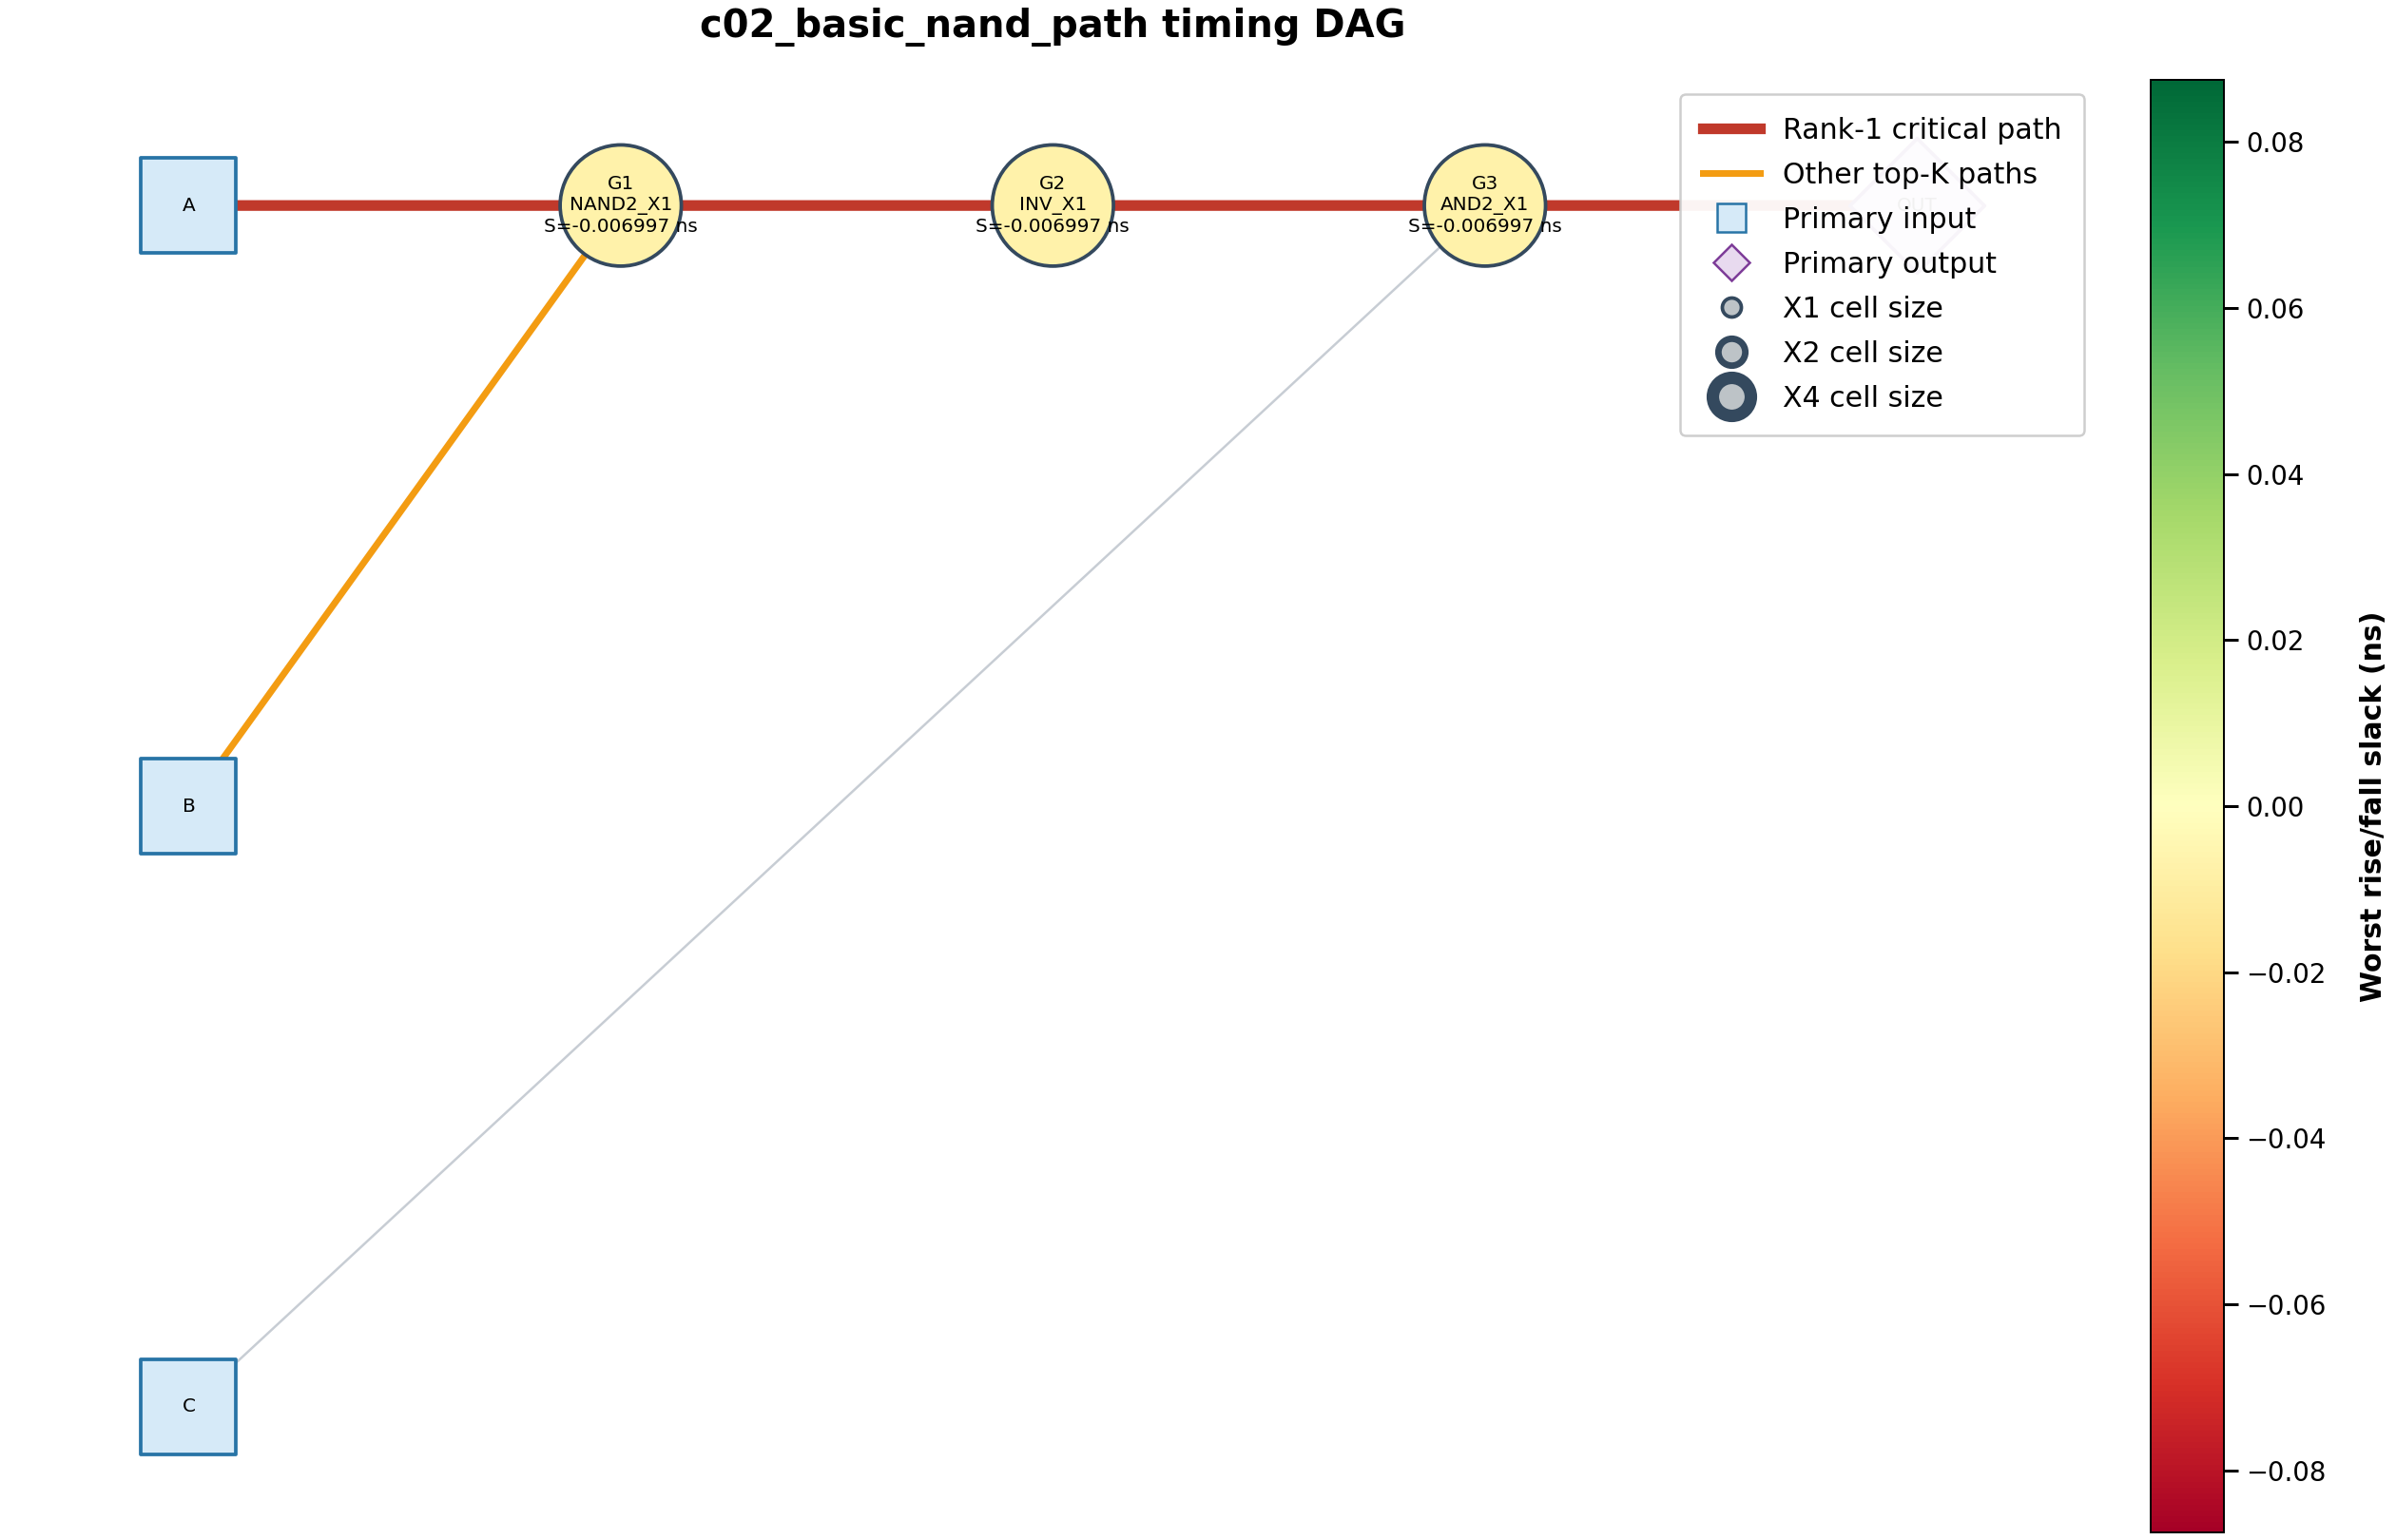
\includegraphics[width=\textwidth]{c02_basic_nand_path_pre.png}
        \caption{Pre-optimization}
    \end{subfigure}
    \hfill
    \begin{subfigure}[t]{0.48\textwidth}
        \centering
        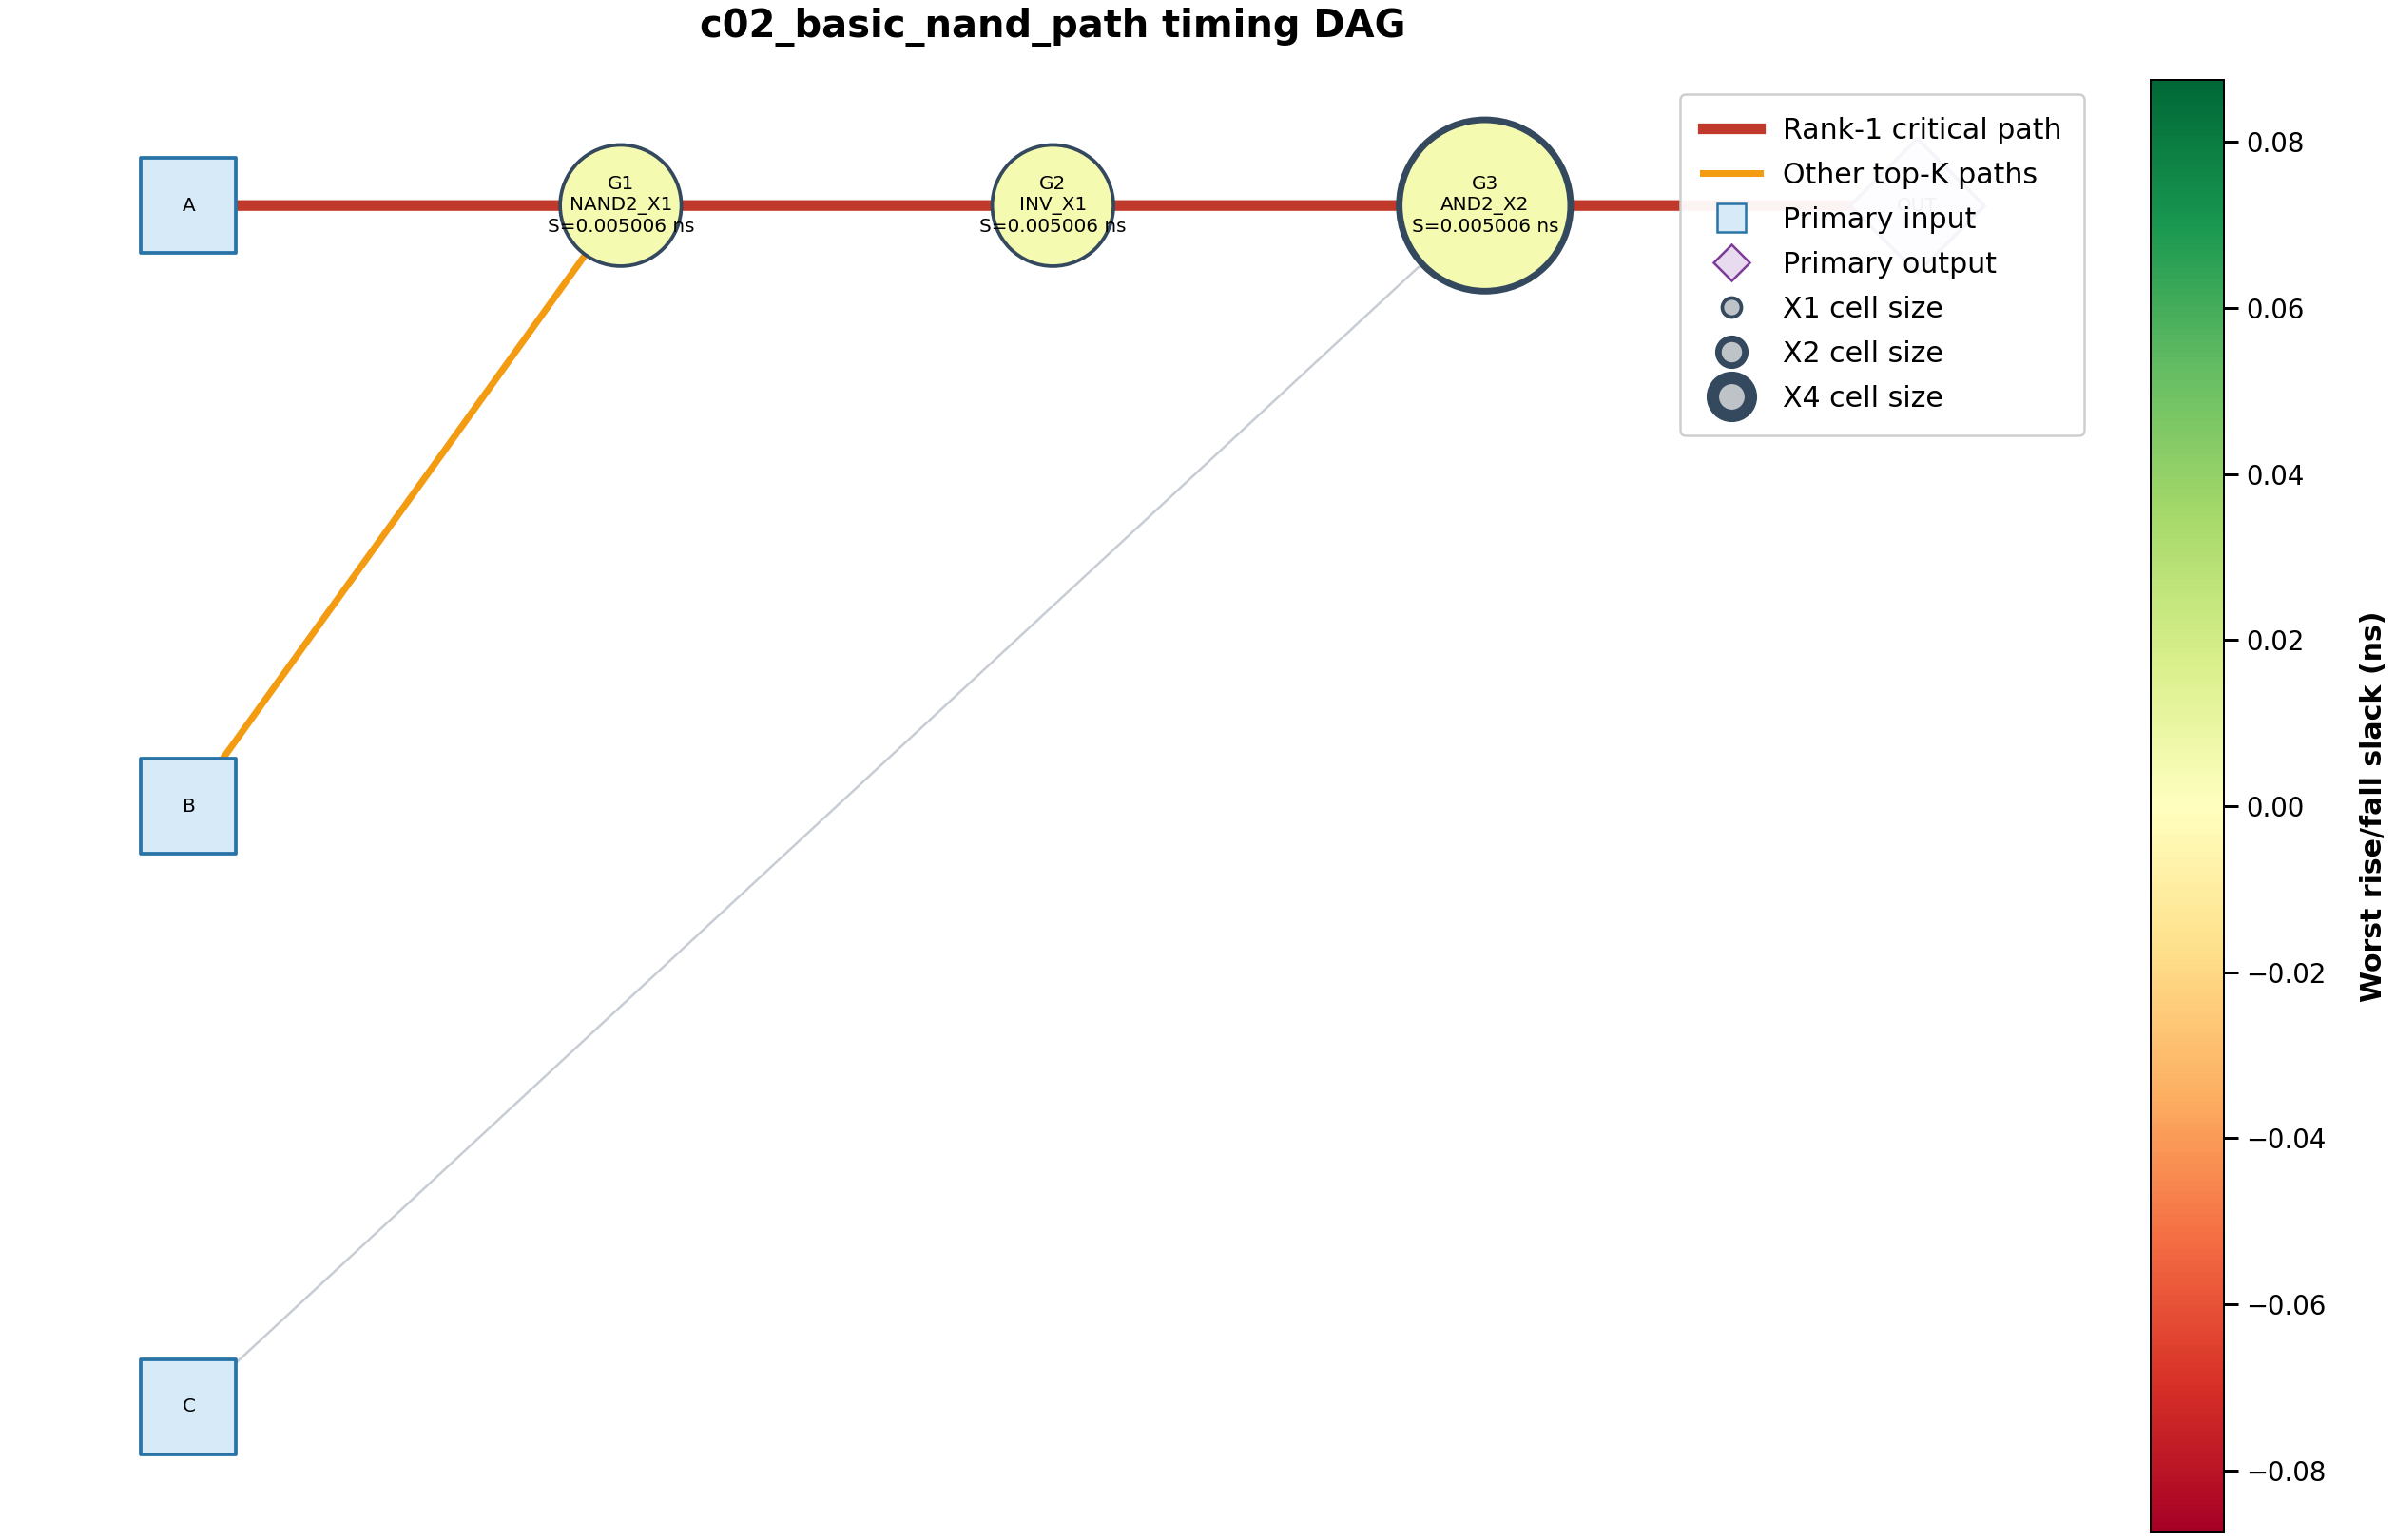
\includegraphics[width=\textwidth]{c02_basic_nand_path_post.png}
        \caption{Post-optimization}
    \end{subfigure}
    \caption{\texttt{c02\_basic\_nand\_path}: circuit diagrams, nodes colored by slack,
    critical path highlighted.}
    \label{fig:app-c02-basic-nand-path-graphs}
\end{figure}

\begin{figure}[H]
    \centering
    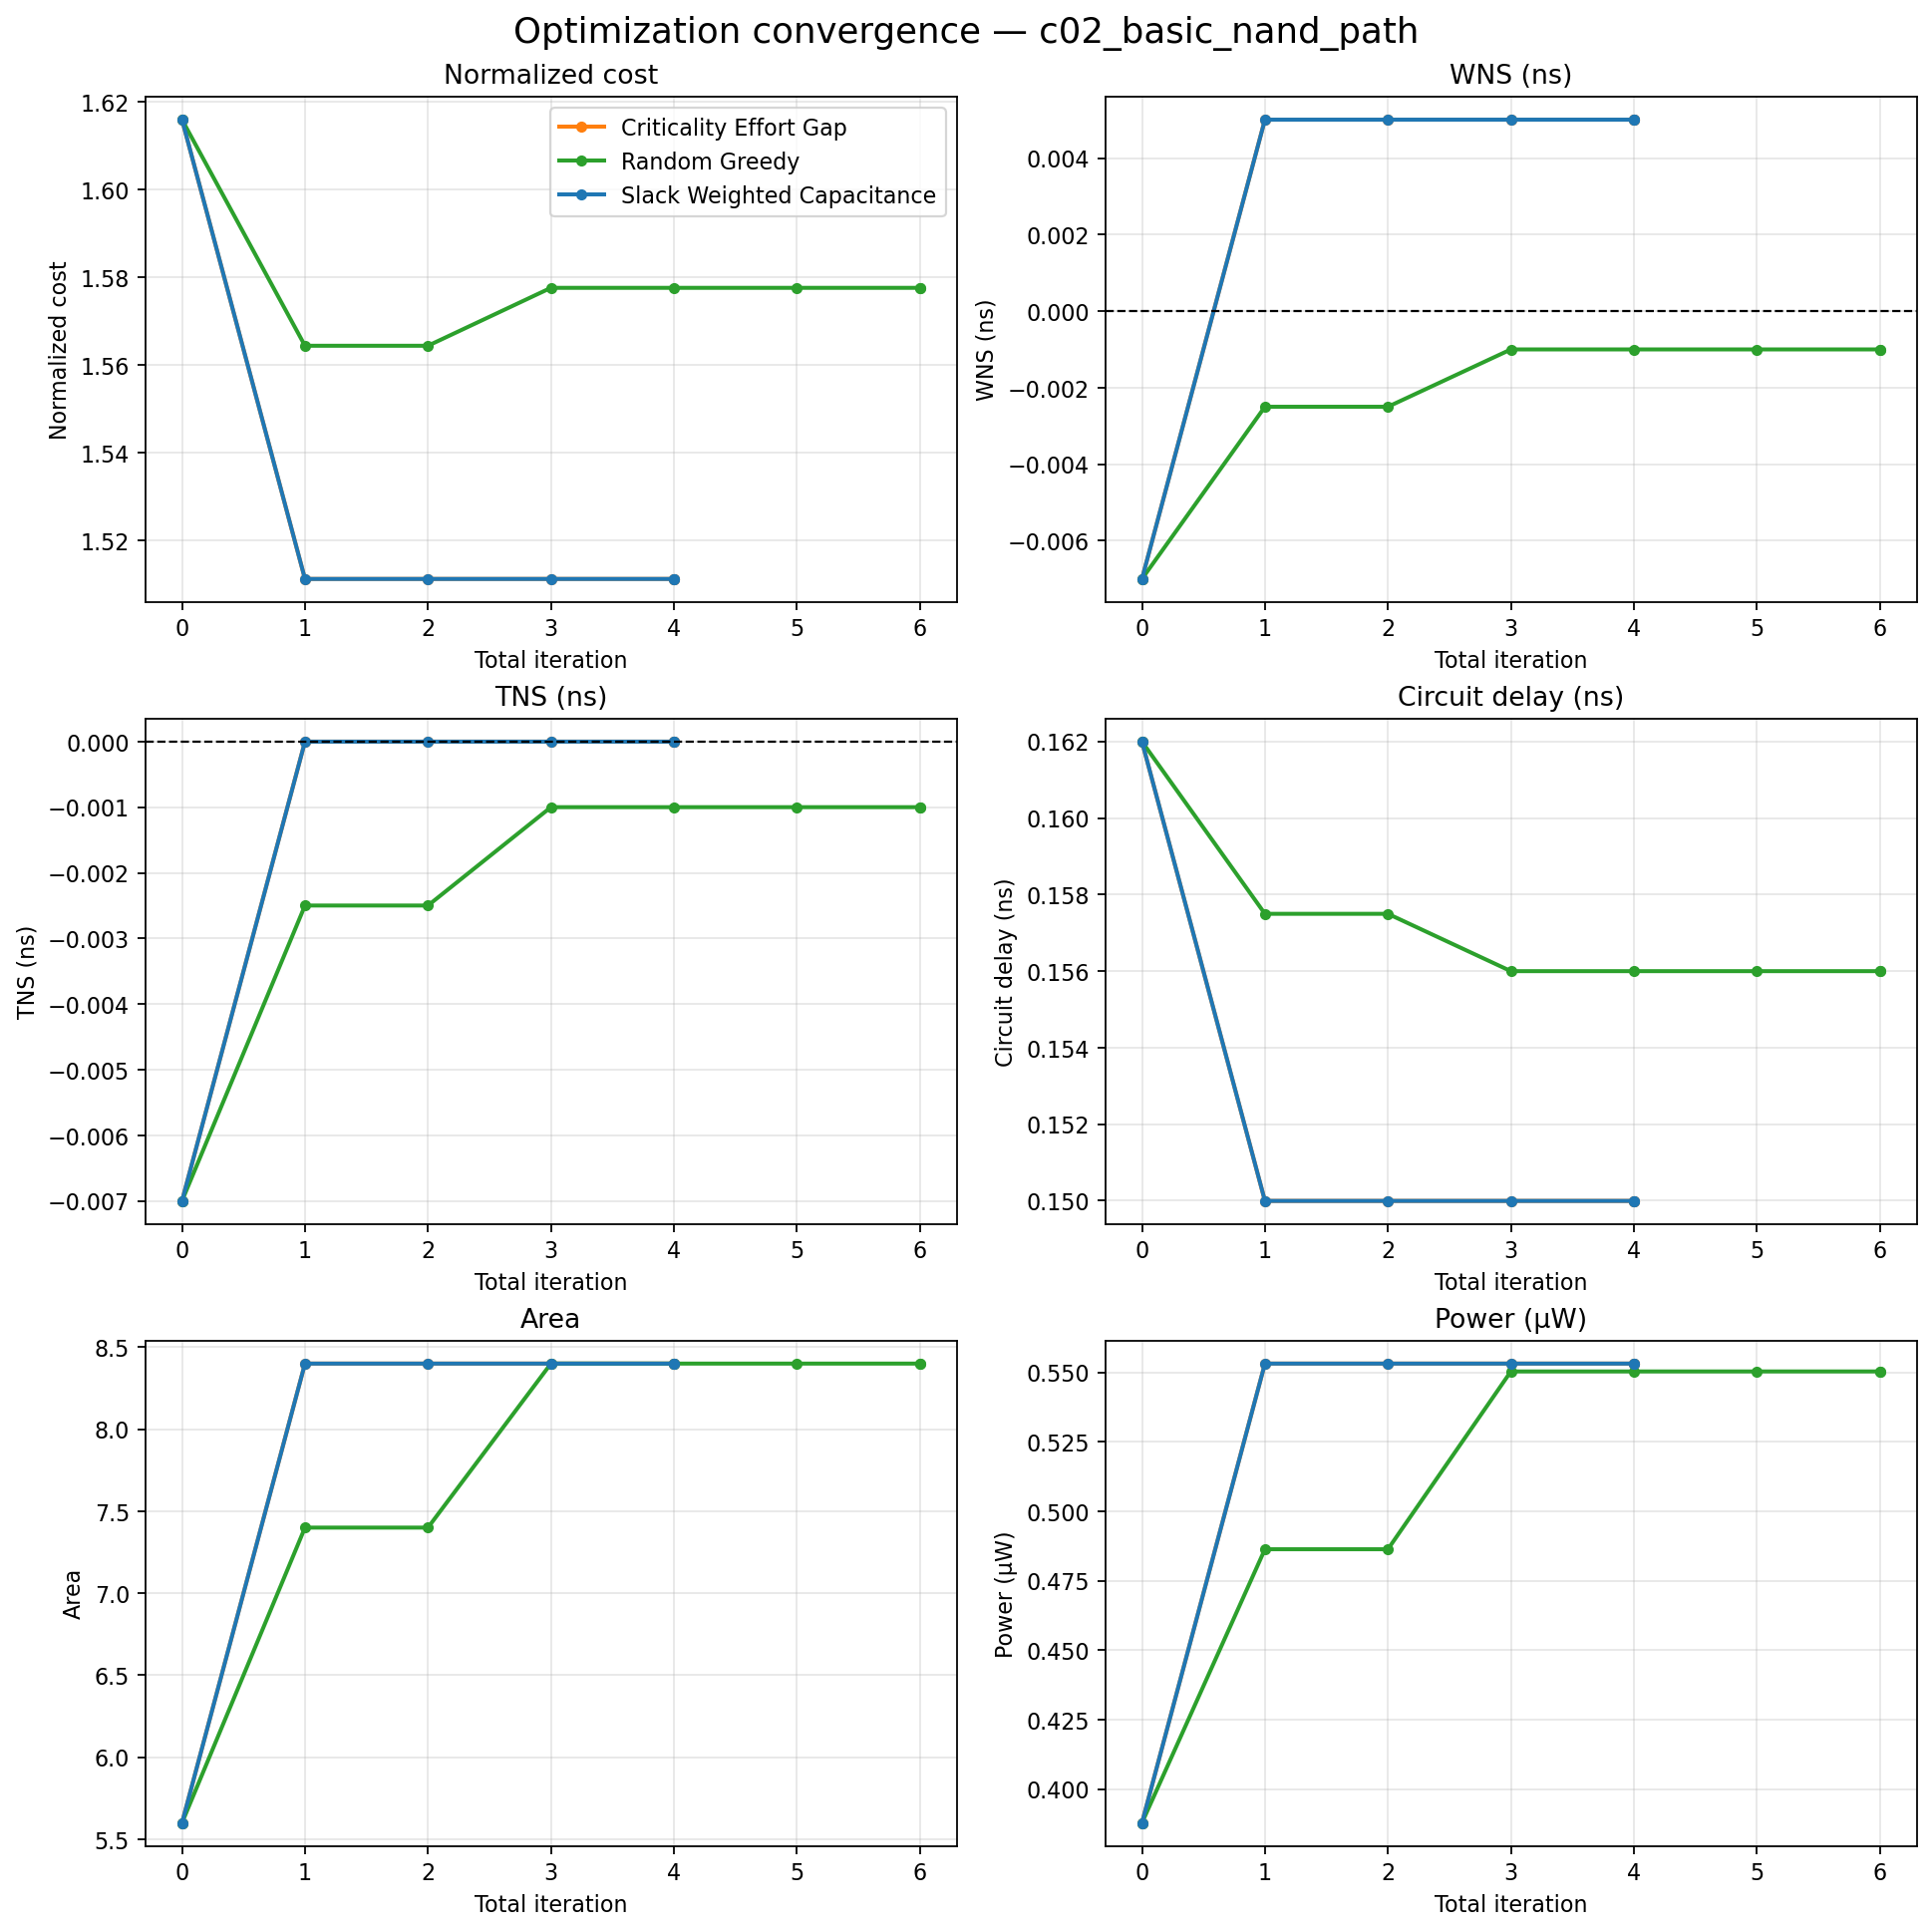
\includegraphics[width=\textwidth]{c02_basic_nand_path_conv.png}
    \caption{\texttt{c02\_basic\_nand\_path}: optimization convergence trace.}
    \label{fig:app-c02-basic-nand-path-conv}
\end{figure}

\begin{figure}[H]
    \centering
    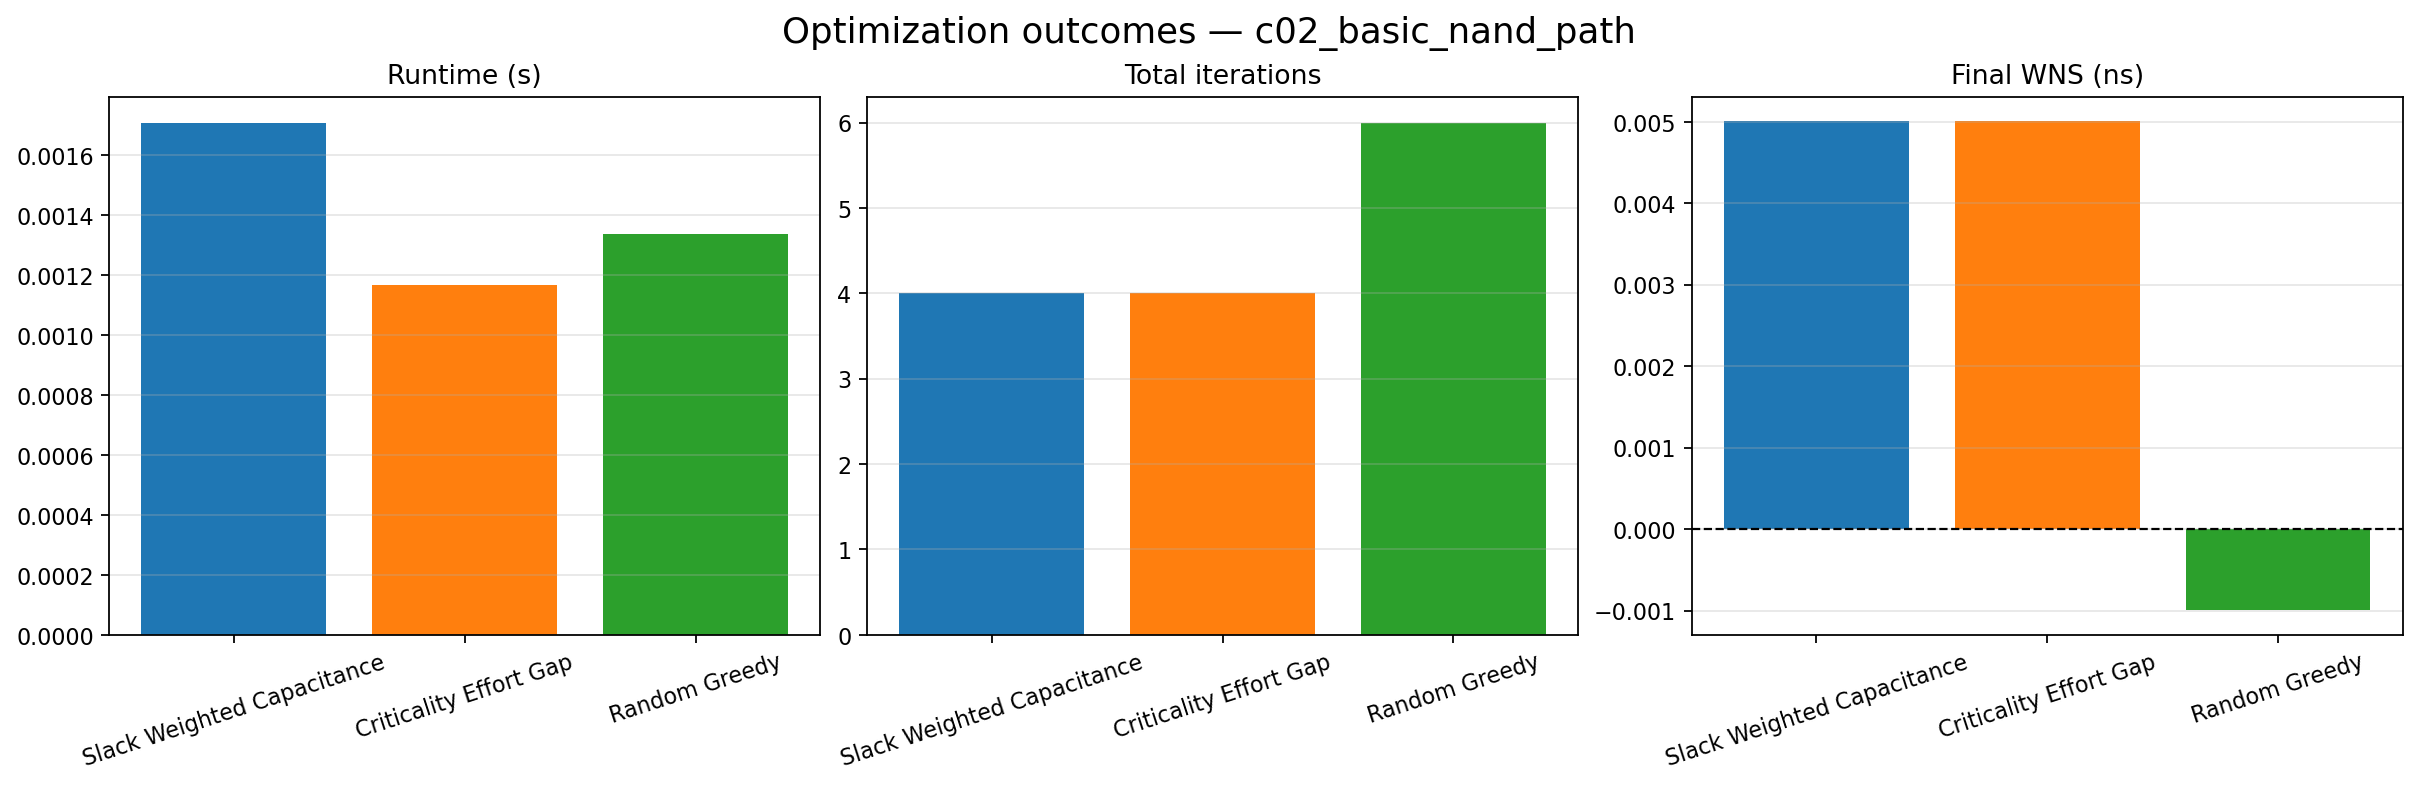
\includegraphics[width=\textwidth]{c02_basic_nand_path_outc.png}
    \caption{\texttt{c02\_basic\_nand\_path}: optimization outcomes summary.}
    \label{fig:app-c02-basic-nand-path-outc}
\end{figure}

\clearpage

\section{\texttt{c03\_fanout\_branch} (4 gates)}
\label{app:fig-c03-fanout-branch}

\begin{figure}[H]
    \centering
    \begin{subfigure}[t]{0.48\textwidth}
        \centering
        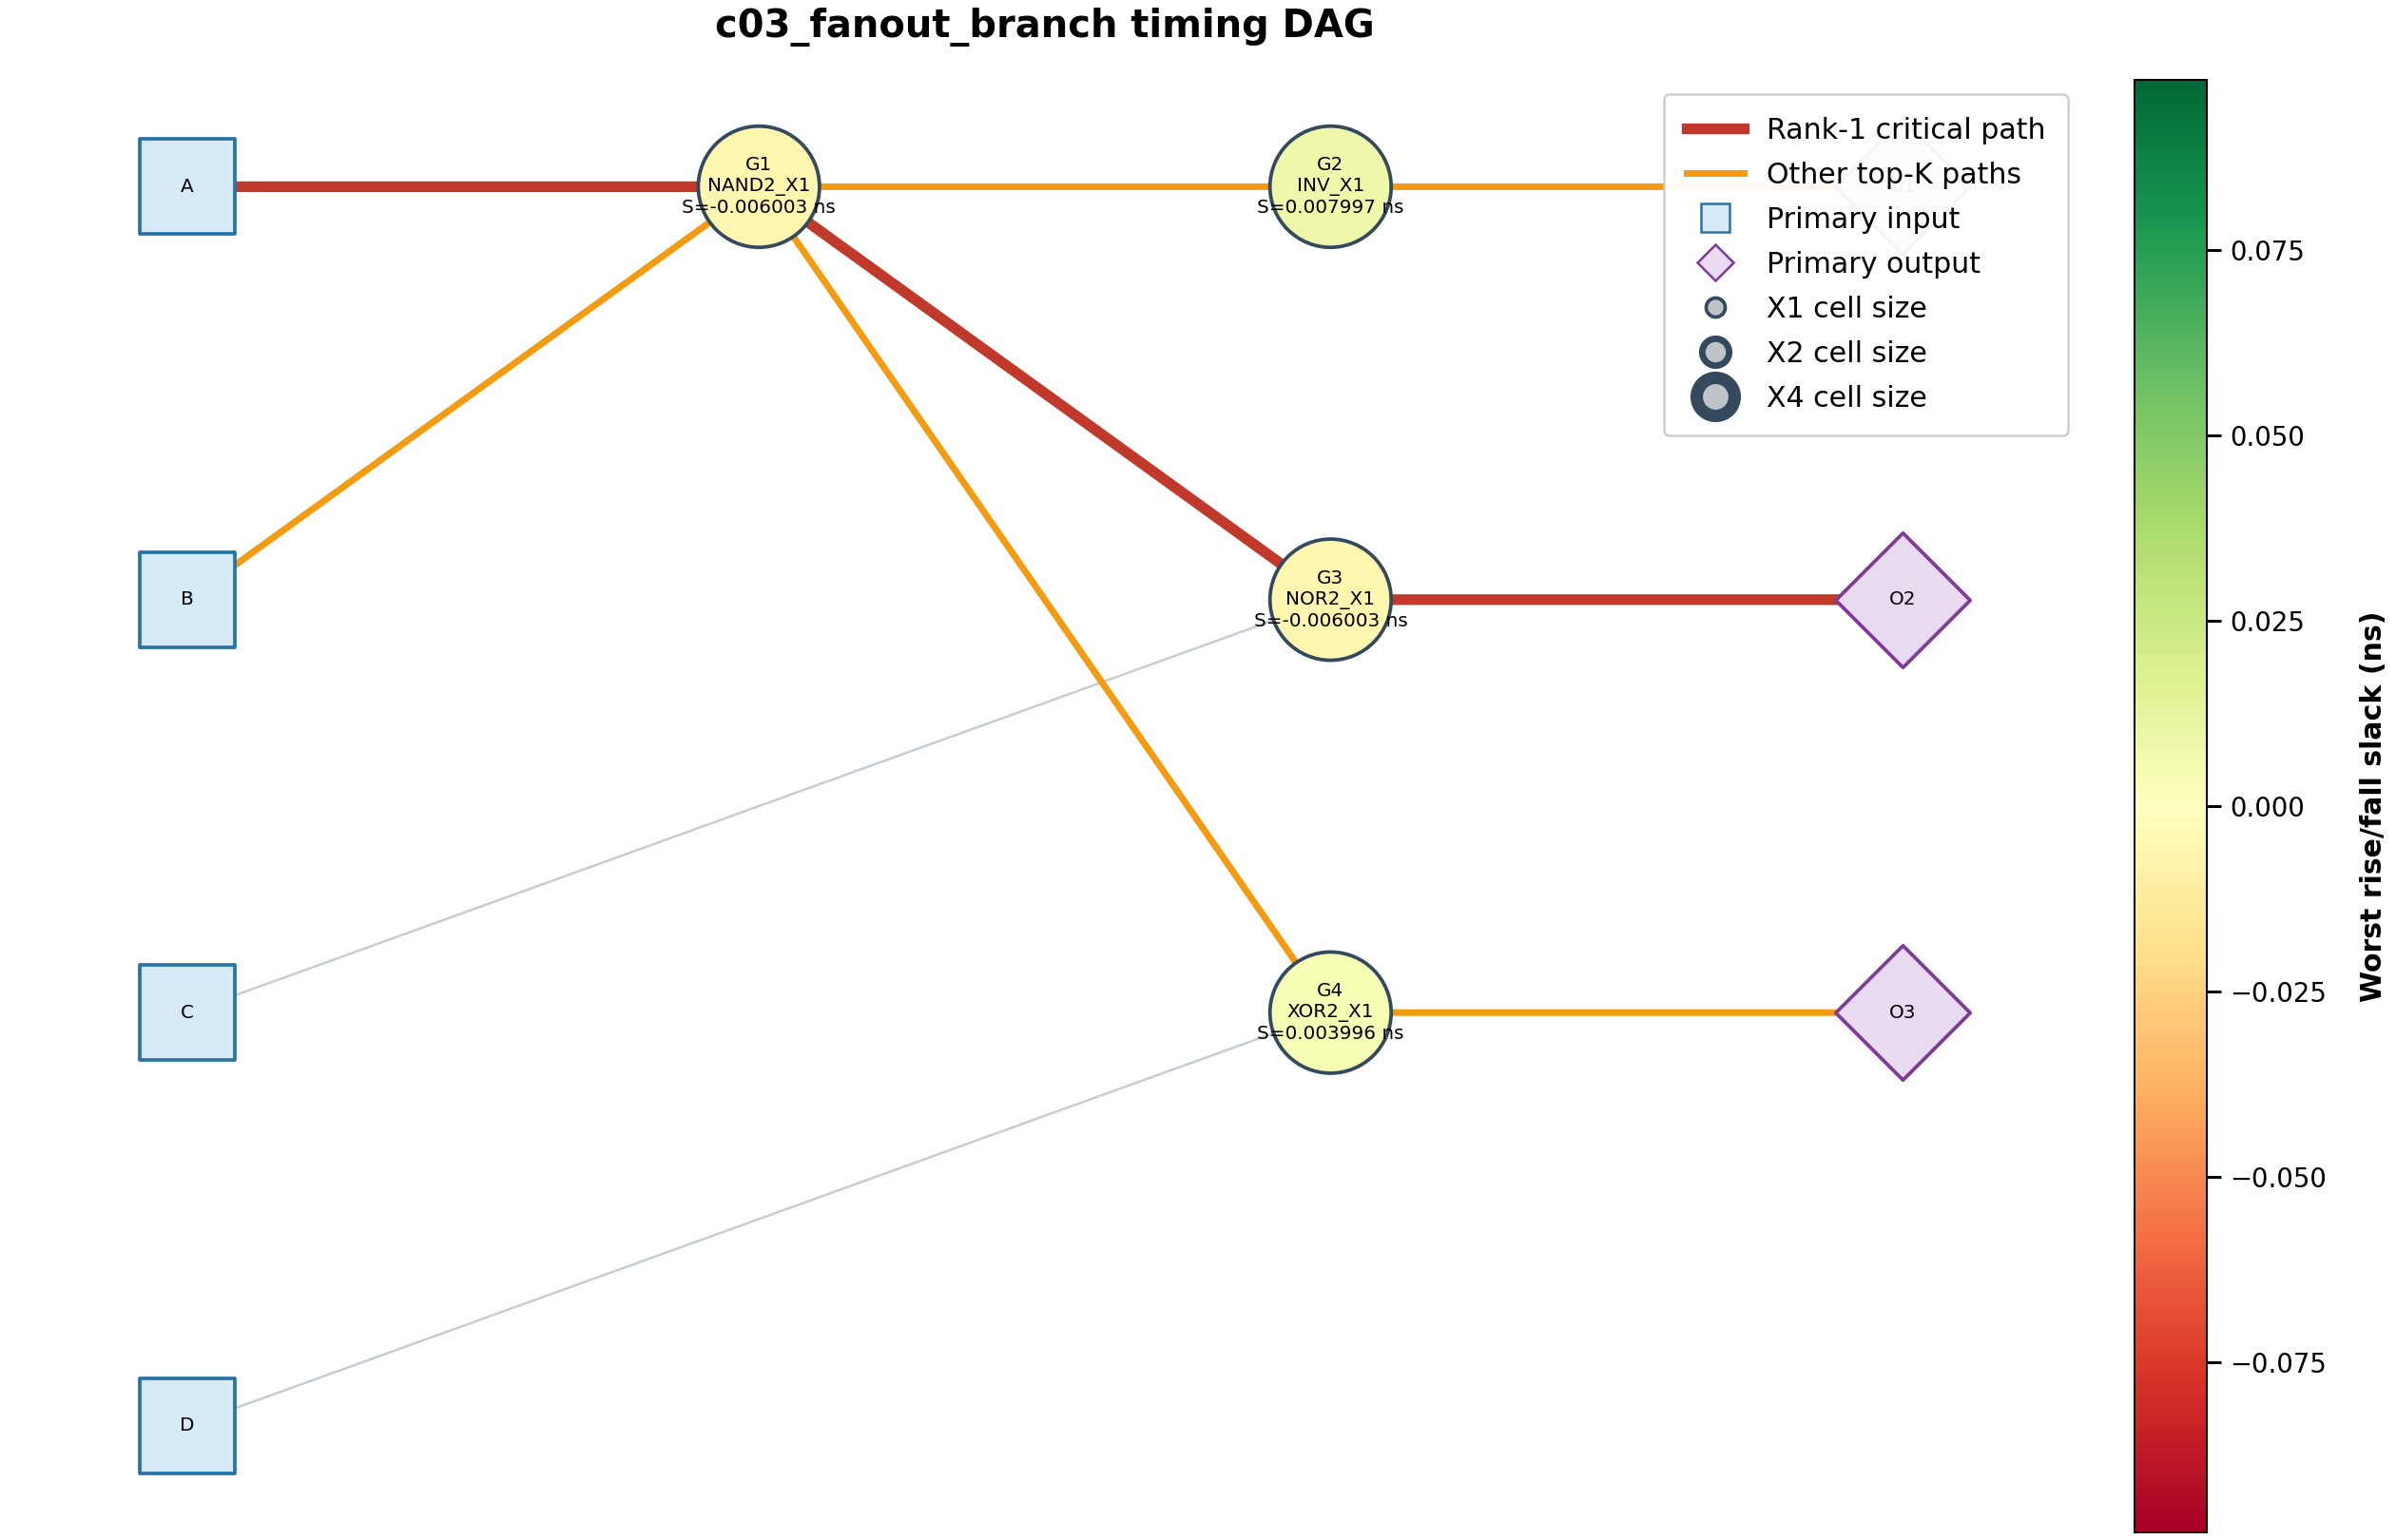
\includegraphics[width=\textwidth]{c03_fanout_branch_pre.png}
        \caption{Pre-optimization}
    \end{subfigure}
    \hfill
    \begin{subfigure}[t]{0.48\textwidth}
        \centering
        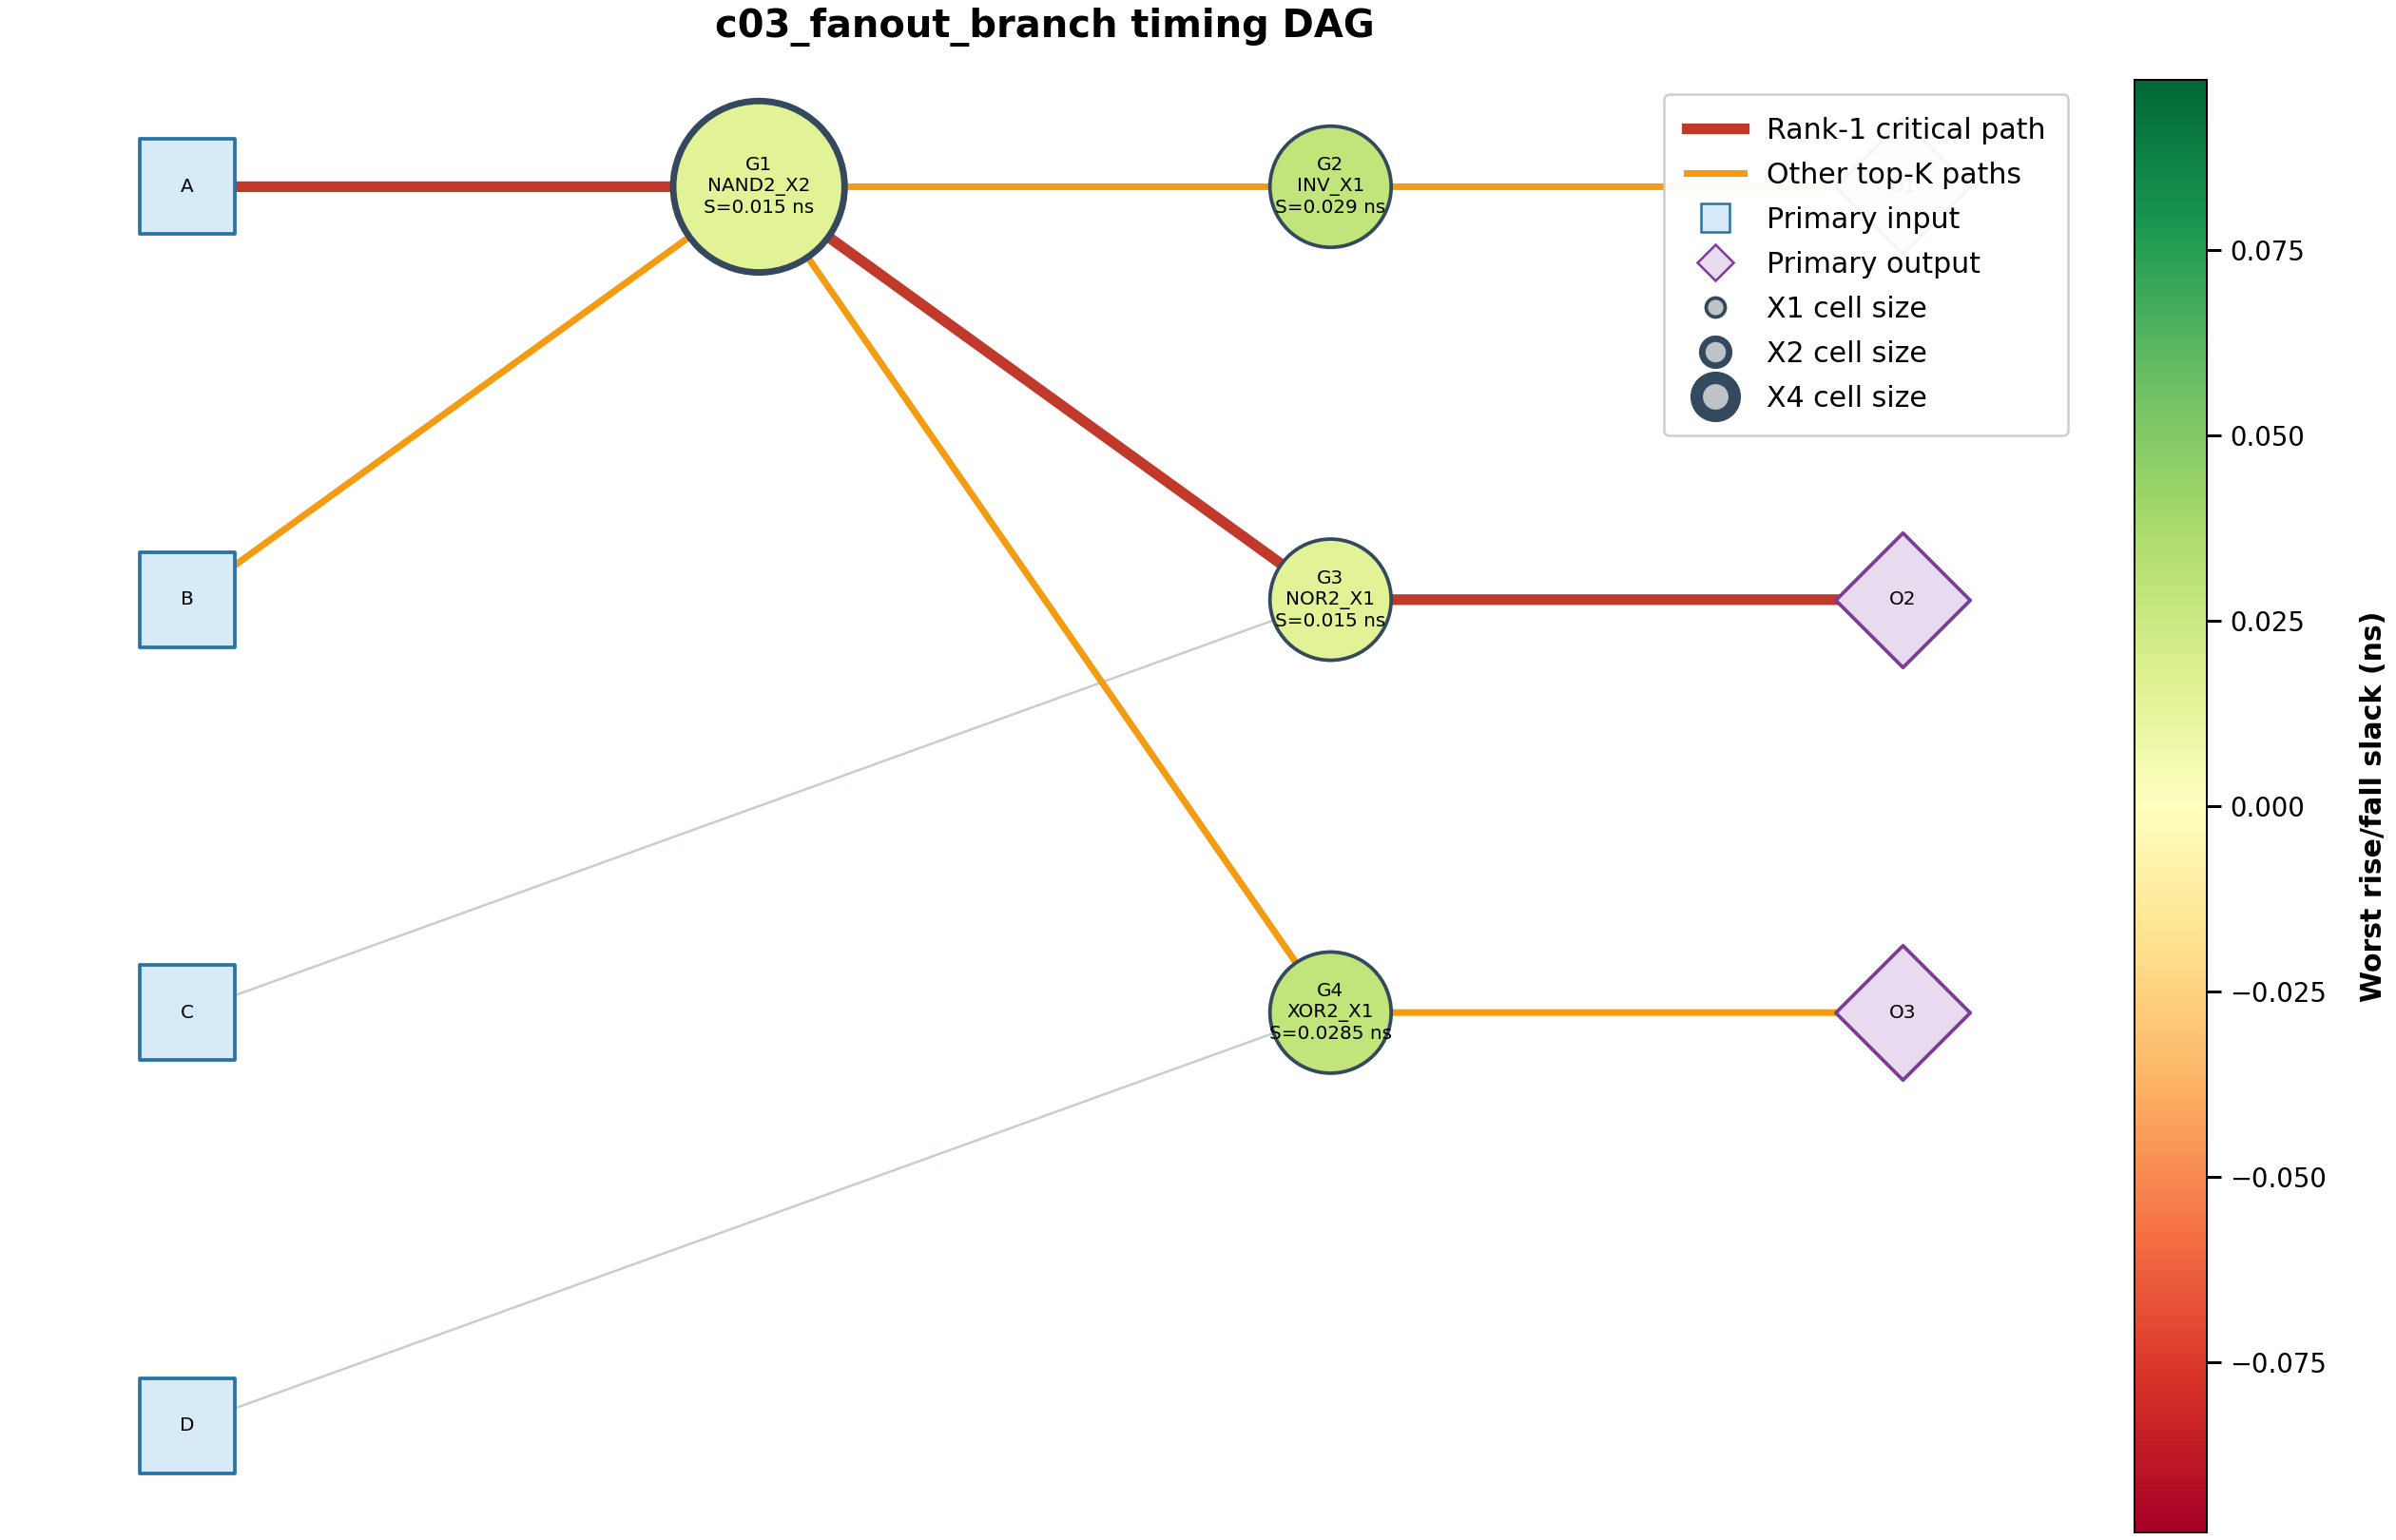
\includegraphics[width=\textwidth]{c03_fanout_branch_post.png}
        \caption{Post-optimization}
    \end{subfigure}
    \caption{\texttt{c03\_fanout\_branch}: circuit diagrams, nodes colored by slack,
    critical path highlighted.}
    \label{fig:app-c03-fanout-branch-graphs}
\end{figure}

\begin{figure}[H]
    \centering
    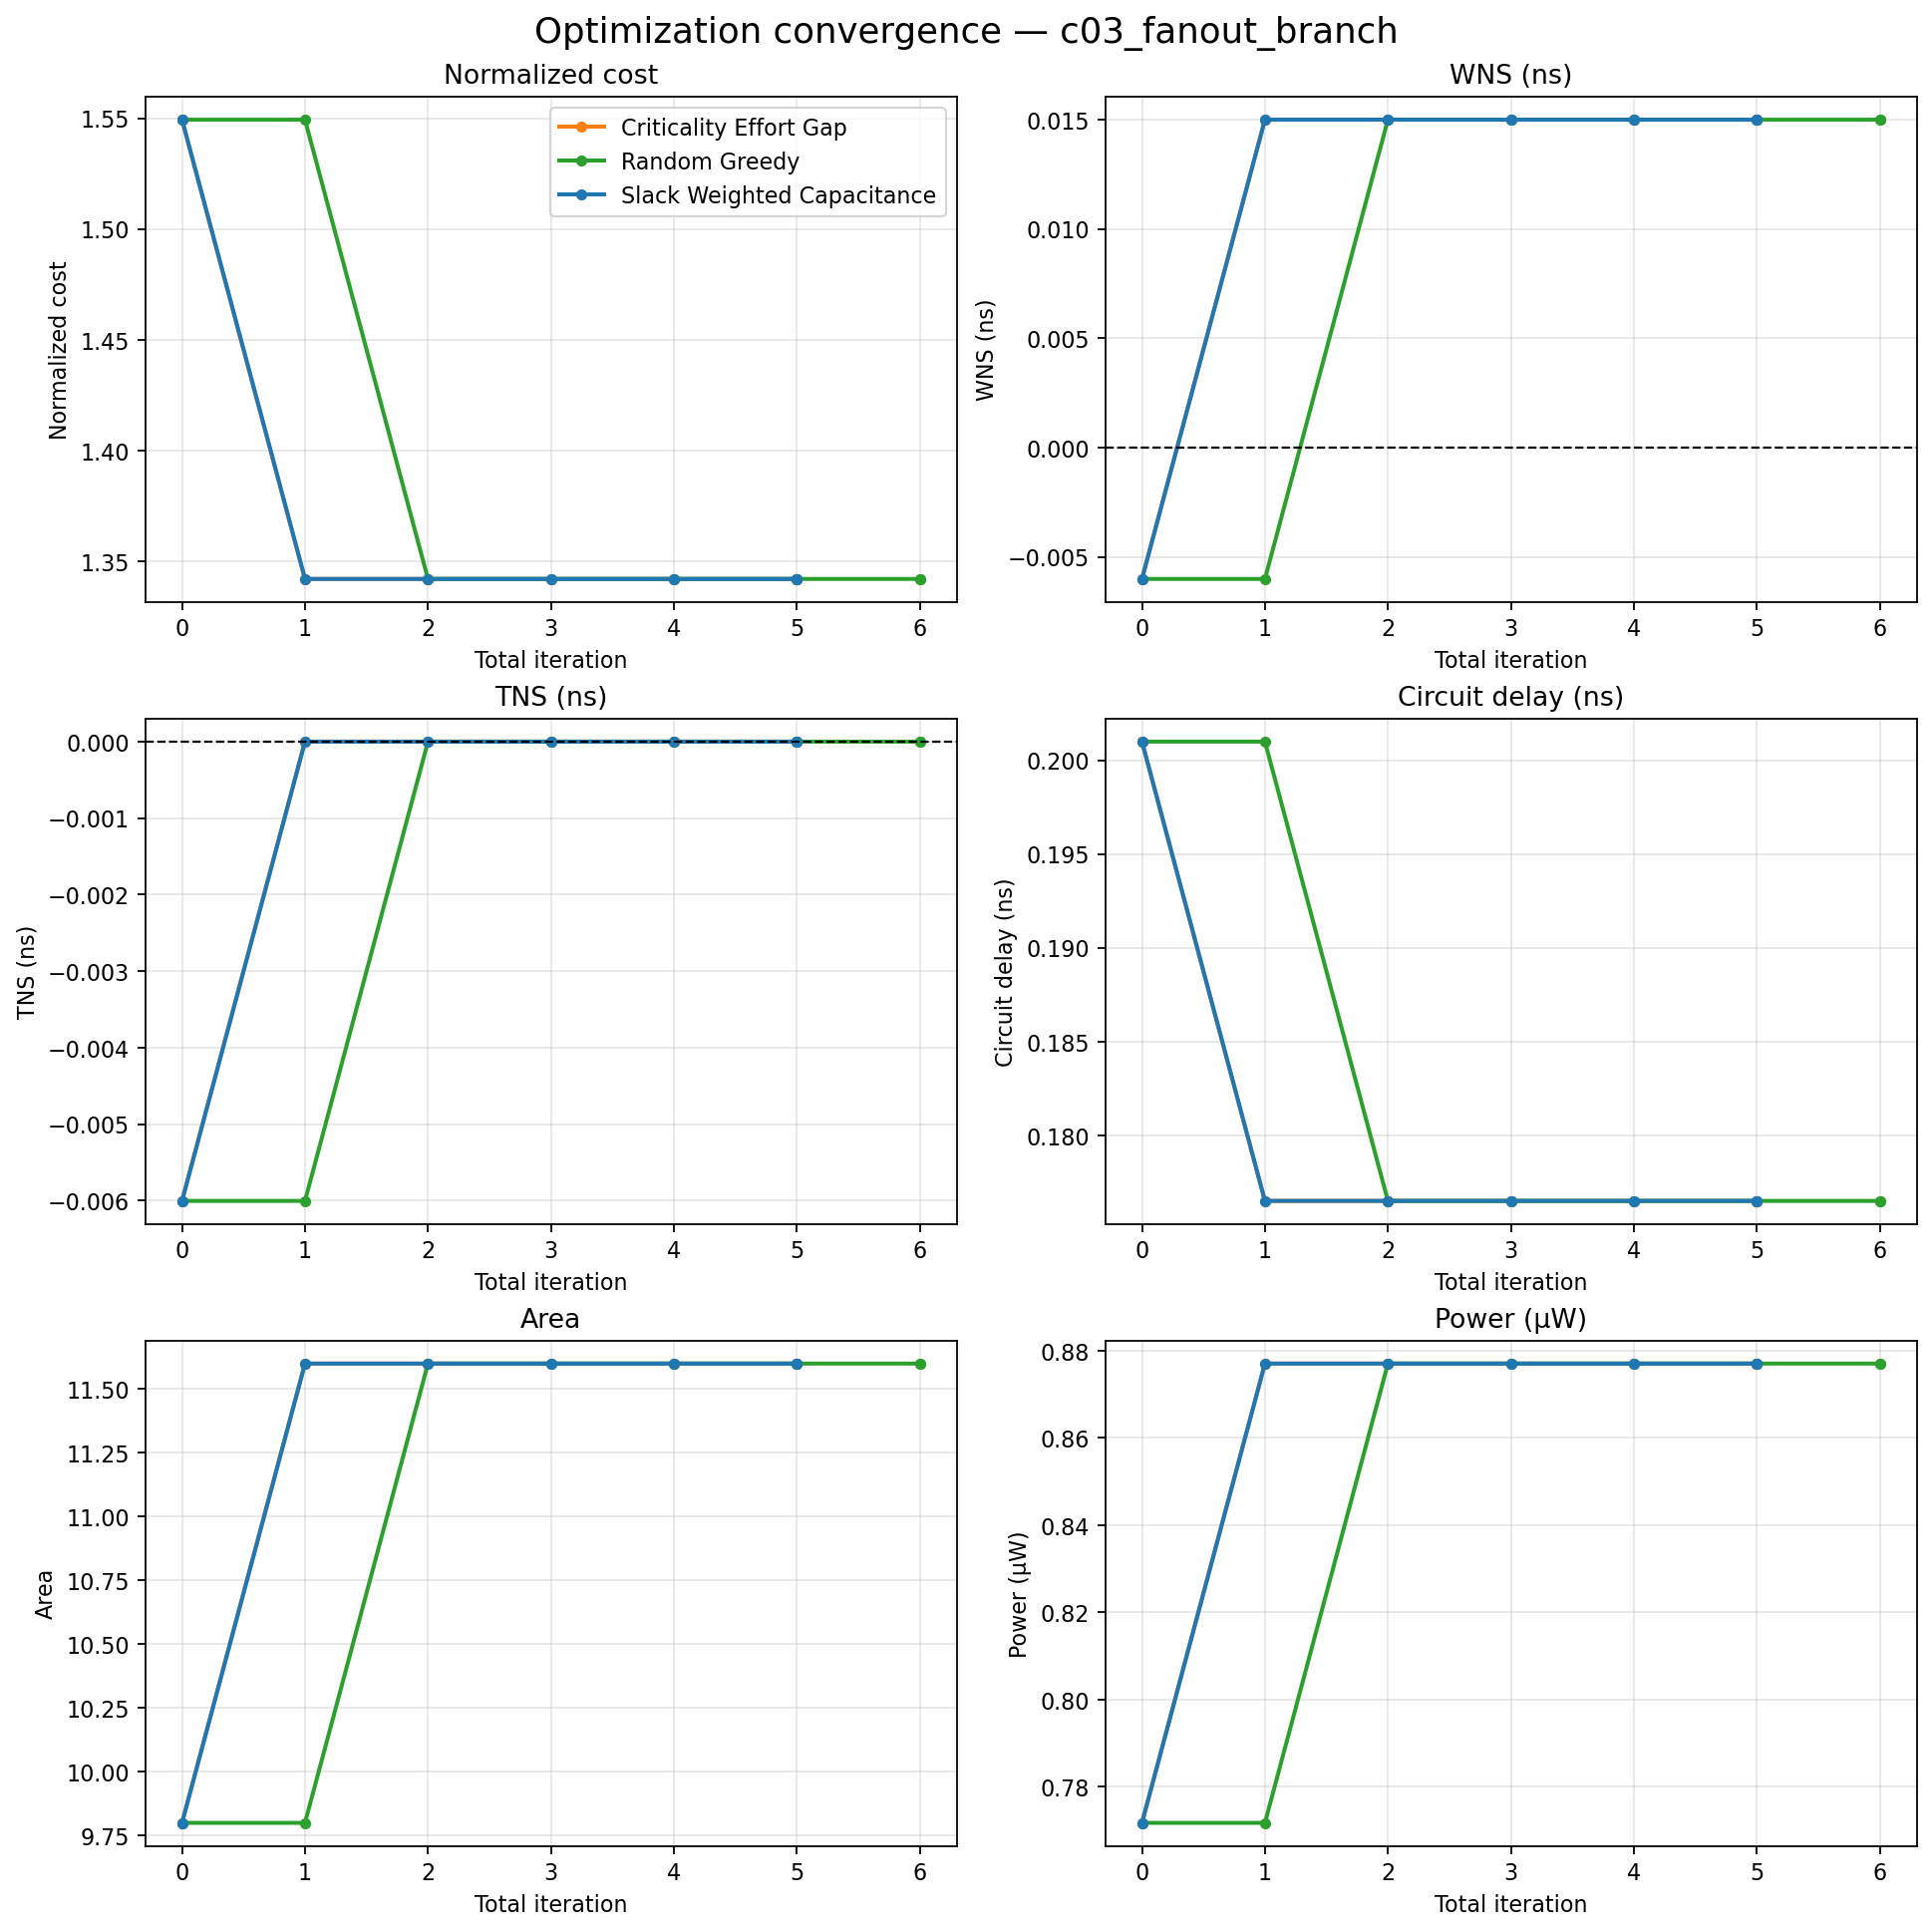
\includegraphics[width=\textwidth]{c03_fanout_branch_conv.png}
    \caption{\texttt{c03\_fanout\_branch}: optimization convergence trace.}
    \label{fig:app-c03-fanout-branch-conv}
\end{figure}

\begin{figure}[H]
    \centering
    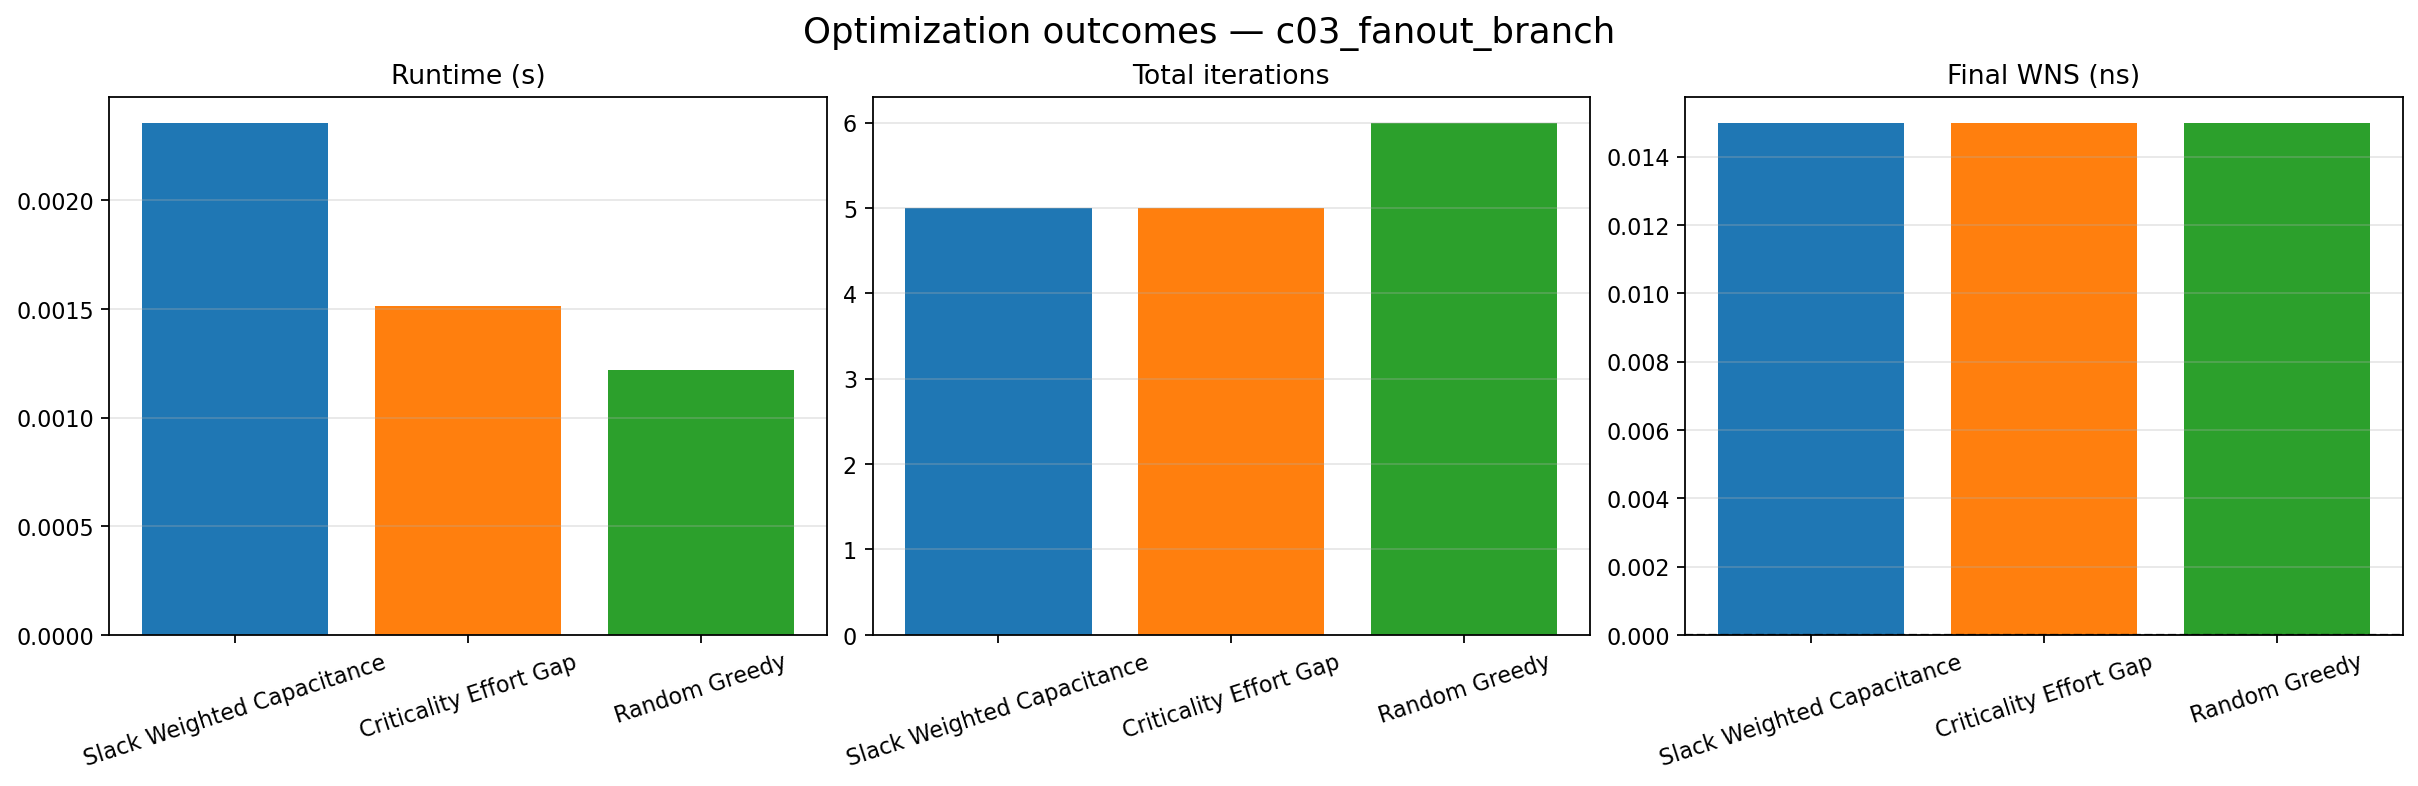
\includegraphics[width=\textwidth]{c03_fanout_branch_outc.png}
    \caption{\texttt{c03\_fanout\_branch}: optimization outcomes summary.}
    \label{fig:app-c03-fanout-branch-outc}
\end{figure}

\clearpage

\section{\texttt{c04\_reconvergent\_paths} (5 gates)}
\label{app:fig-c04-reconvergent-paths}

\begin{figure}[H]
    \centering
    \begin{subfigure}[t]{0.48\textwidth}
        \centering
        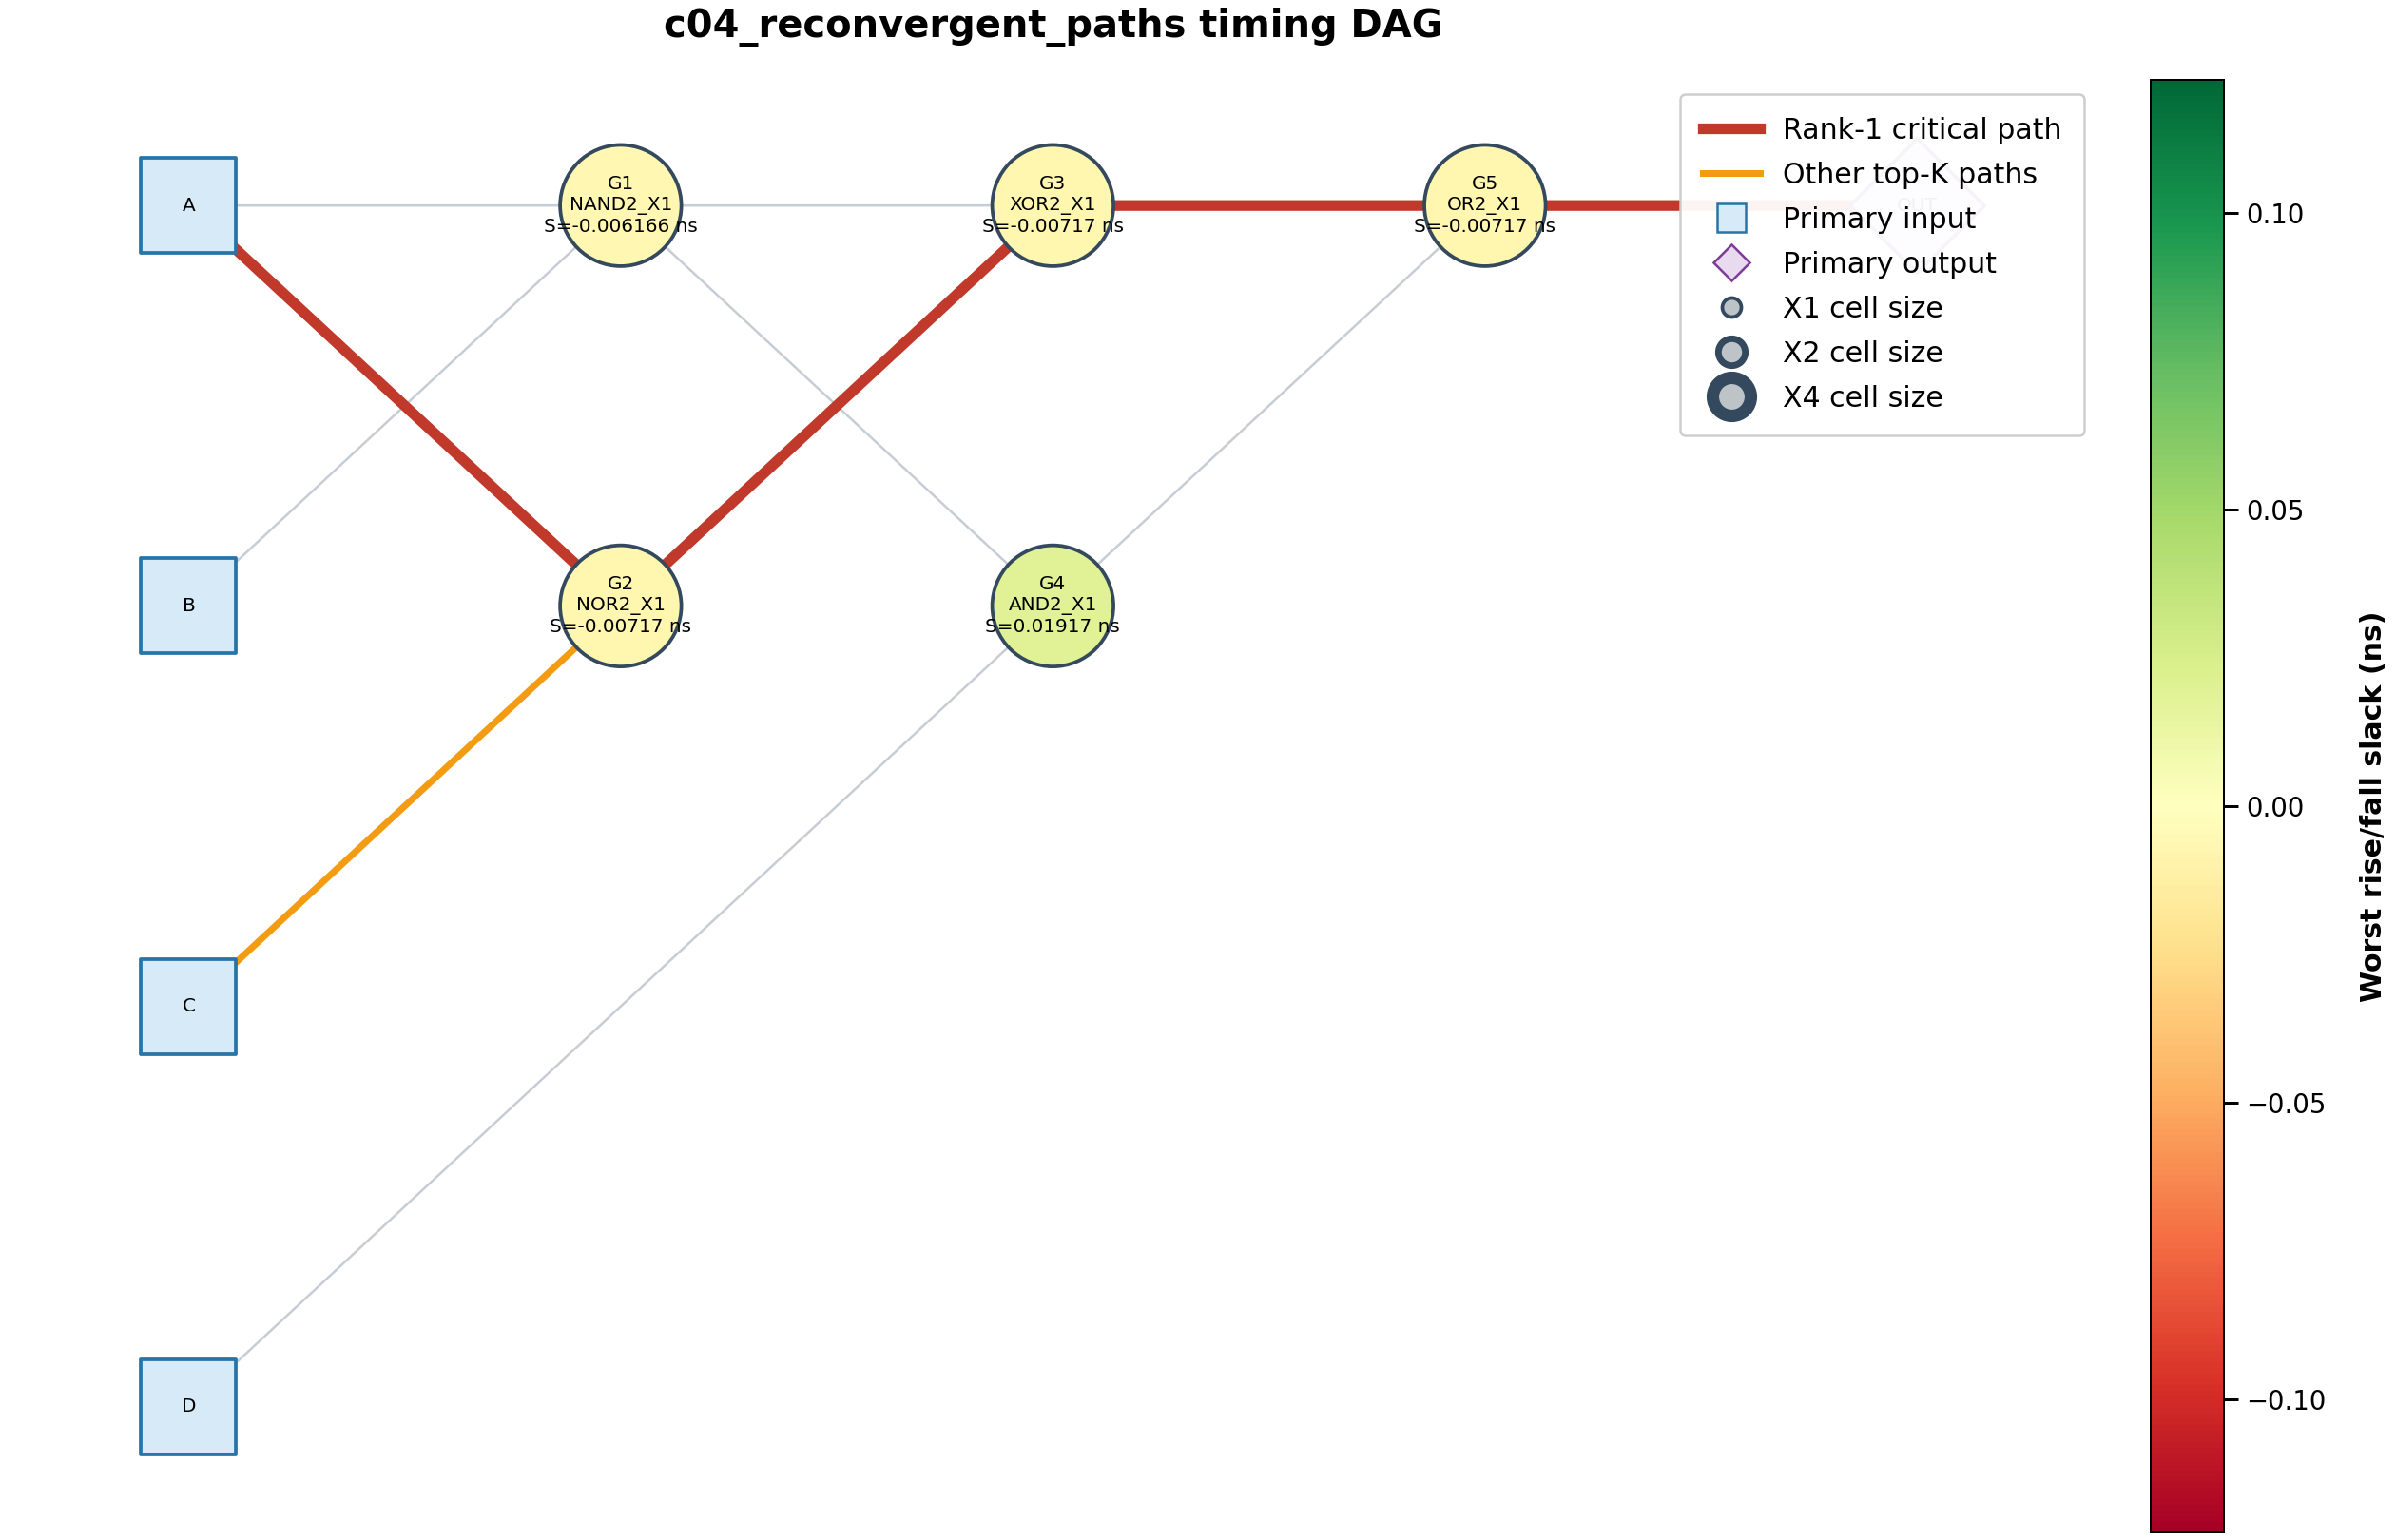
\includegraphics[width=\textwidth]{c04_reconvergent_paths_pre.png}
        \caption{Pre-optimization}
    \end{subfigure}
    \hfill
    \begin{subfigure}[t]{0.48\textwidth}
        \centering
        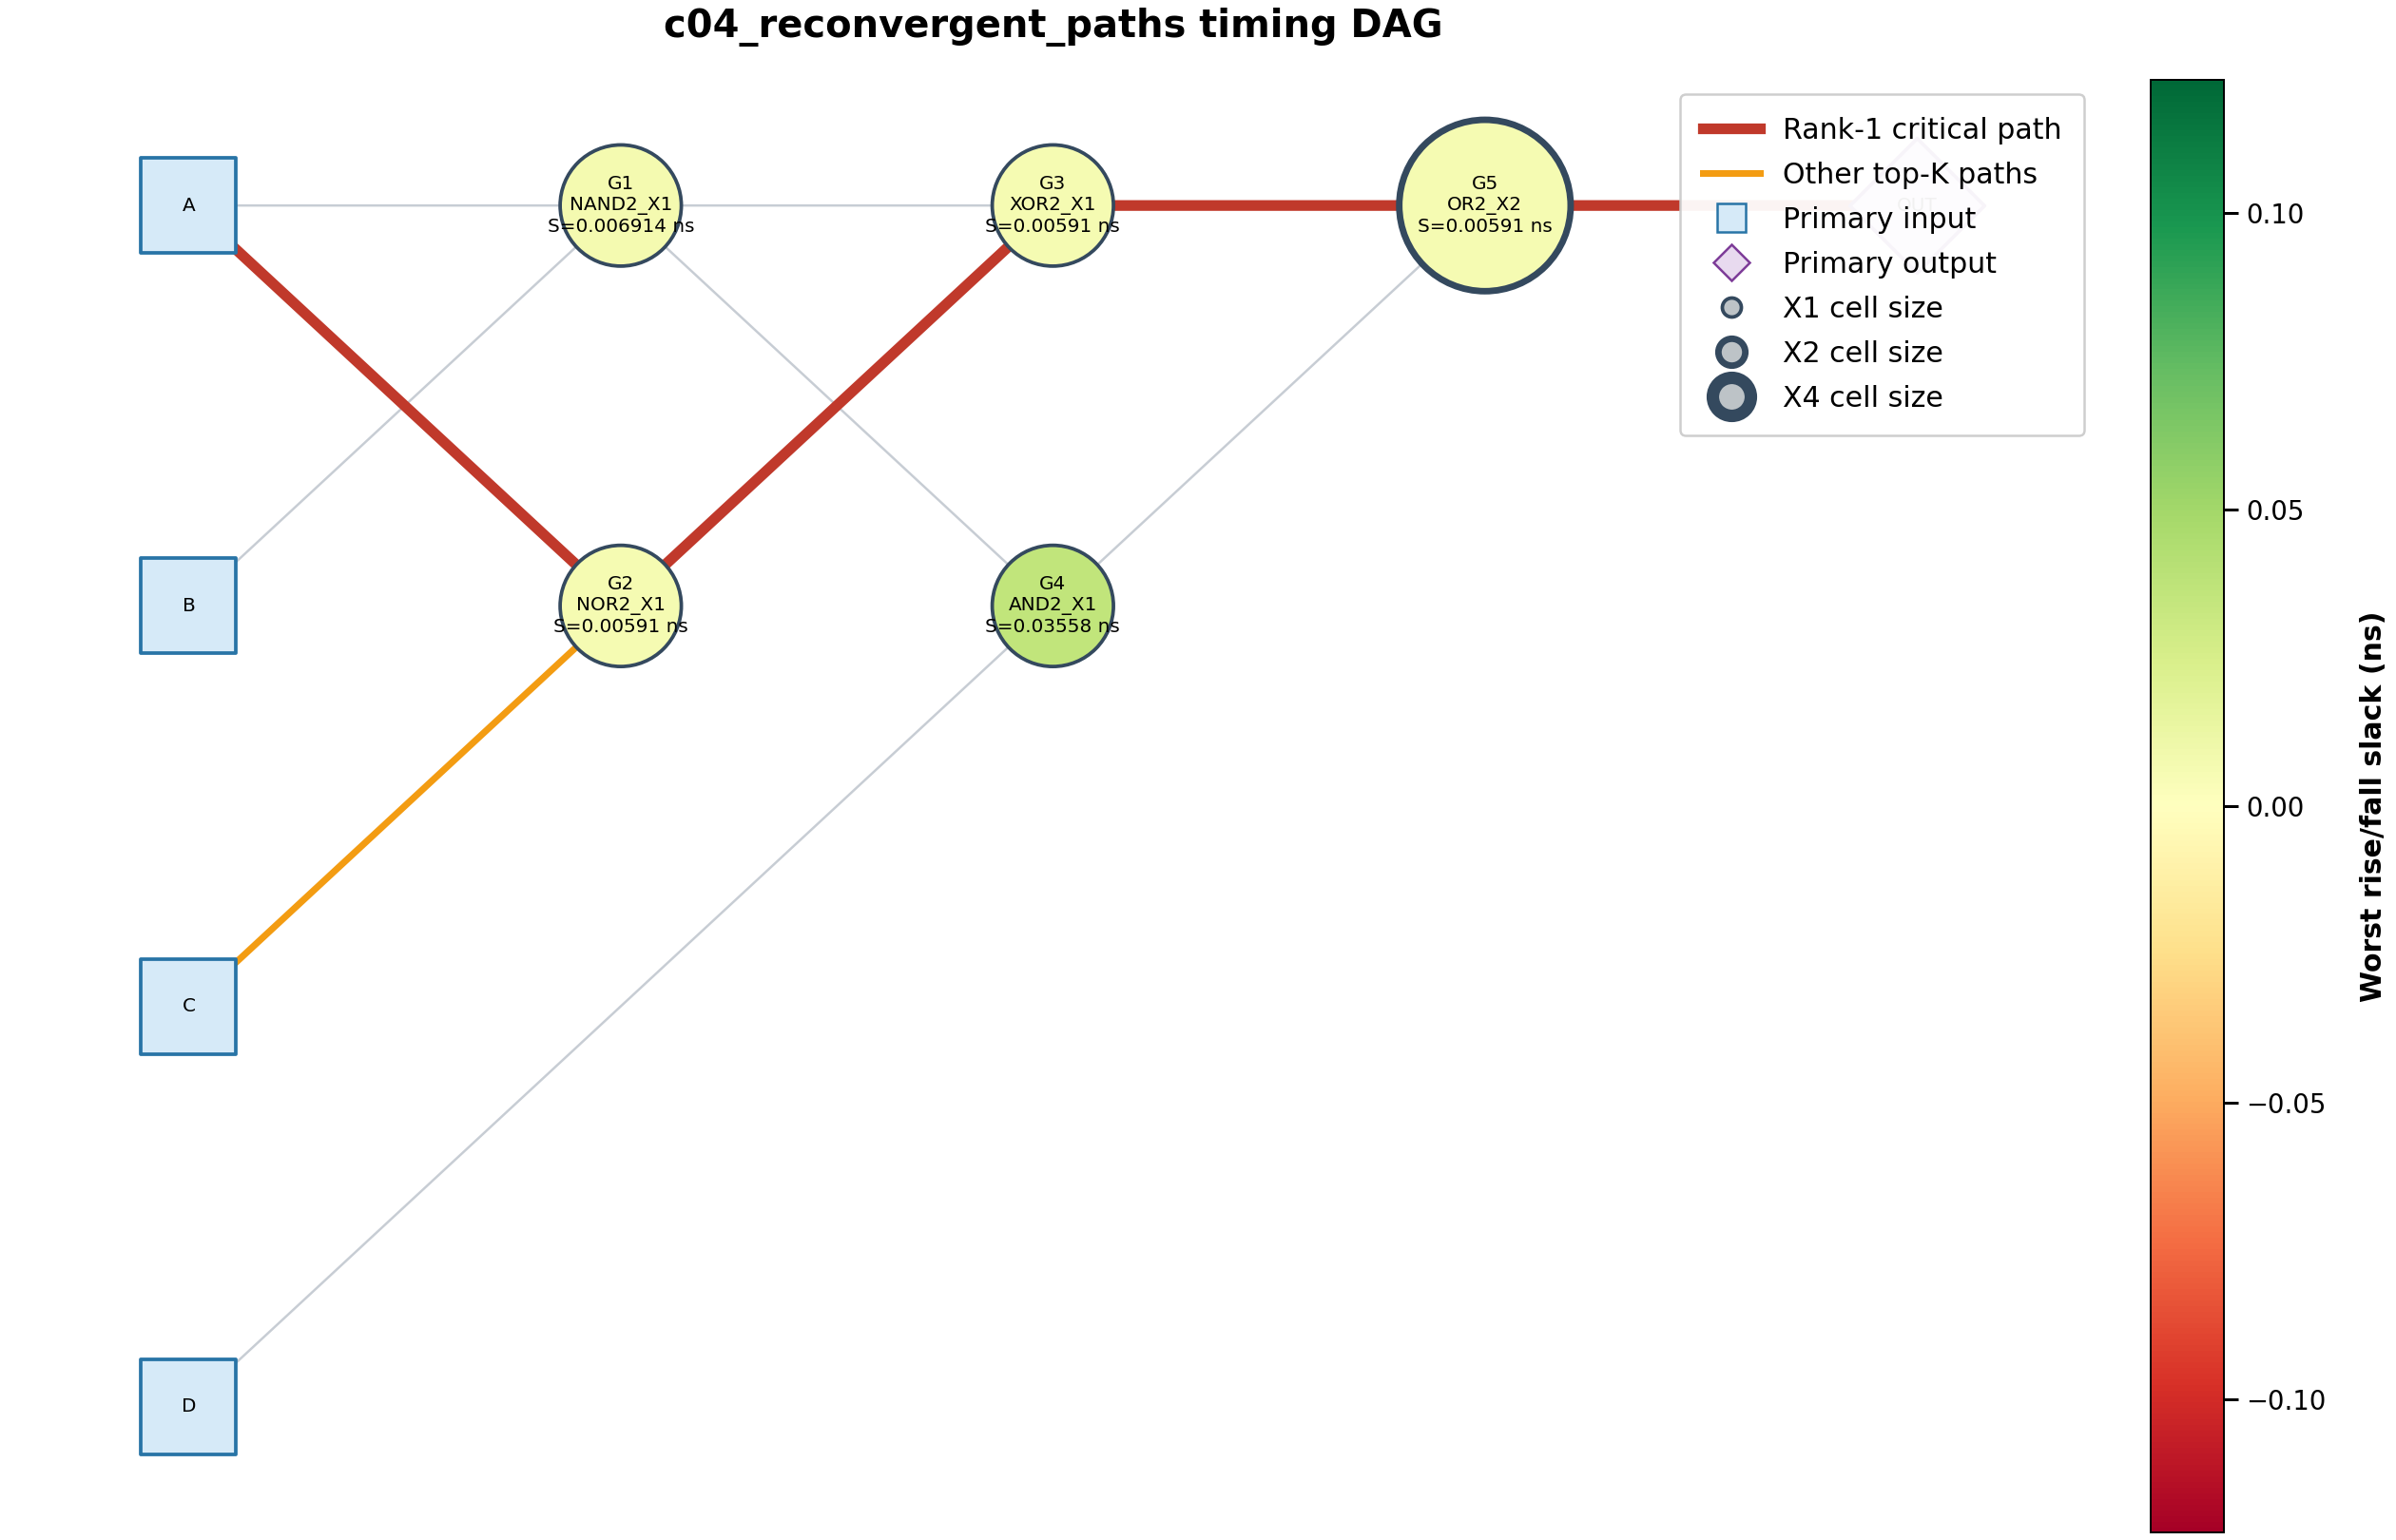
\includegraphics[width=\textwidth]{c04_reconvergent_paths_post.png}
        \caption{Post-optimization}
    \end{subfigure}
    \caption{\texttt{c04\_reconvergent\_paths}: circuit diagrams, nodes colored by slack,
    critical path highlighted.}
    \label{fig:app-c04-reconvergent-paths-graphs}
\end{figure}

\begin{figure}[H]
    \centering
    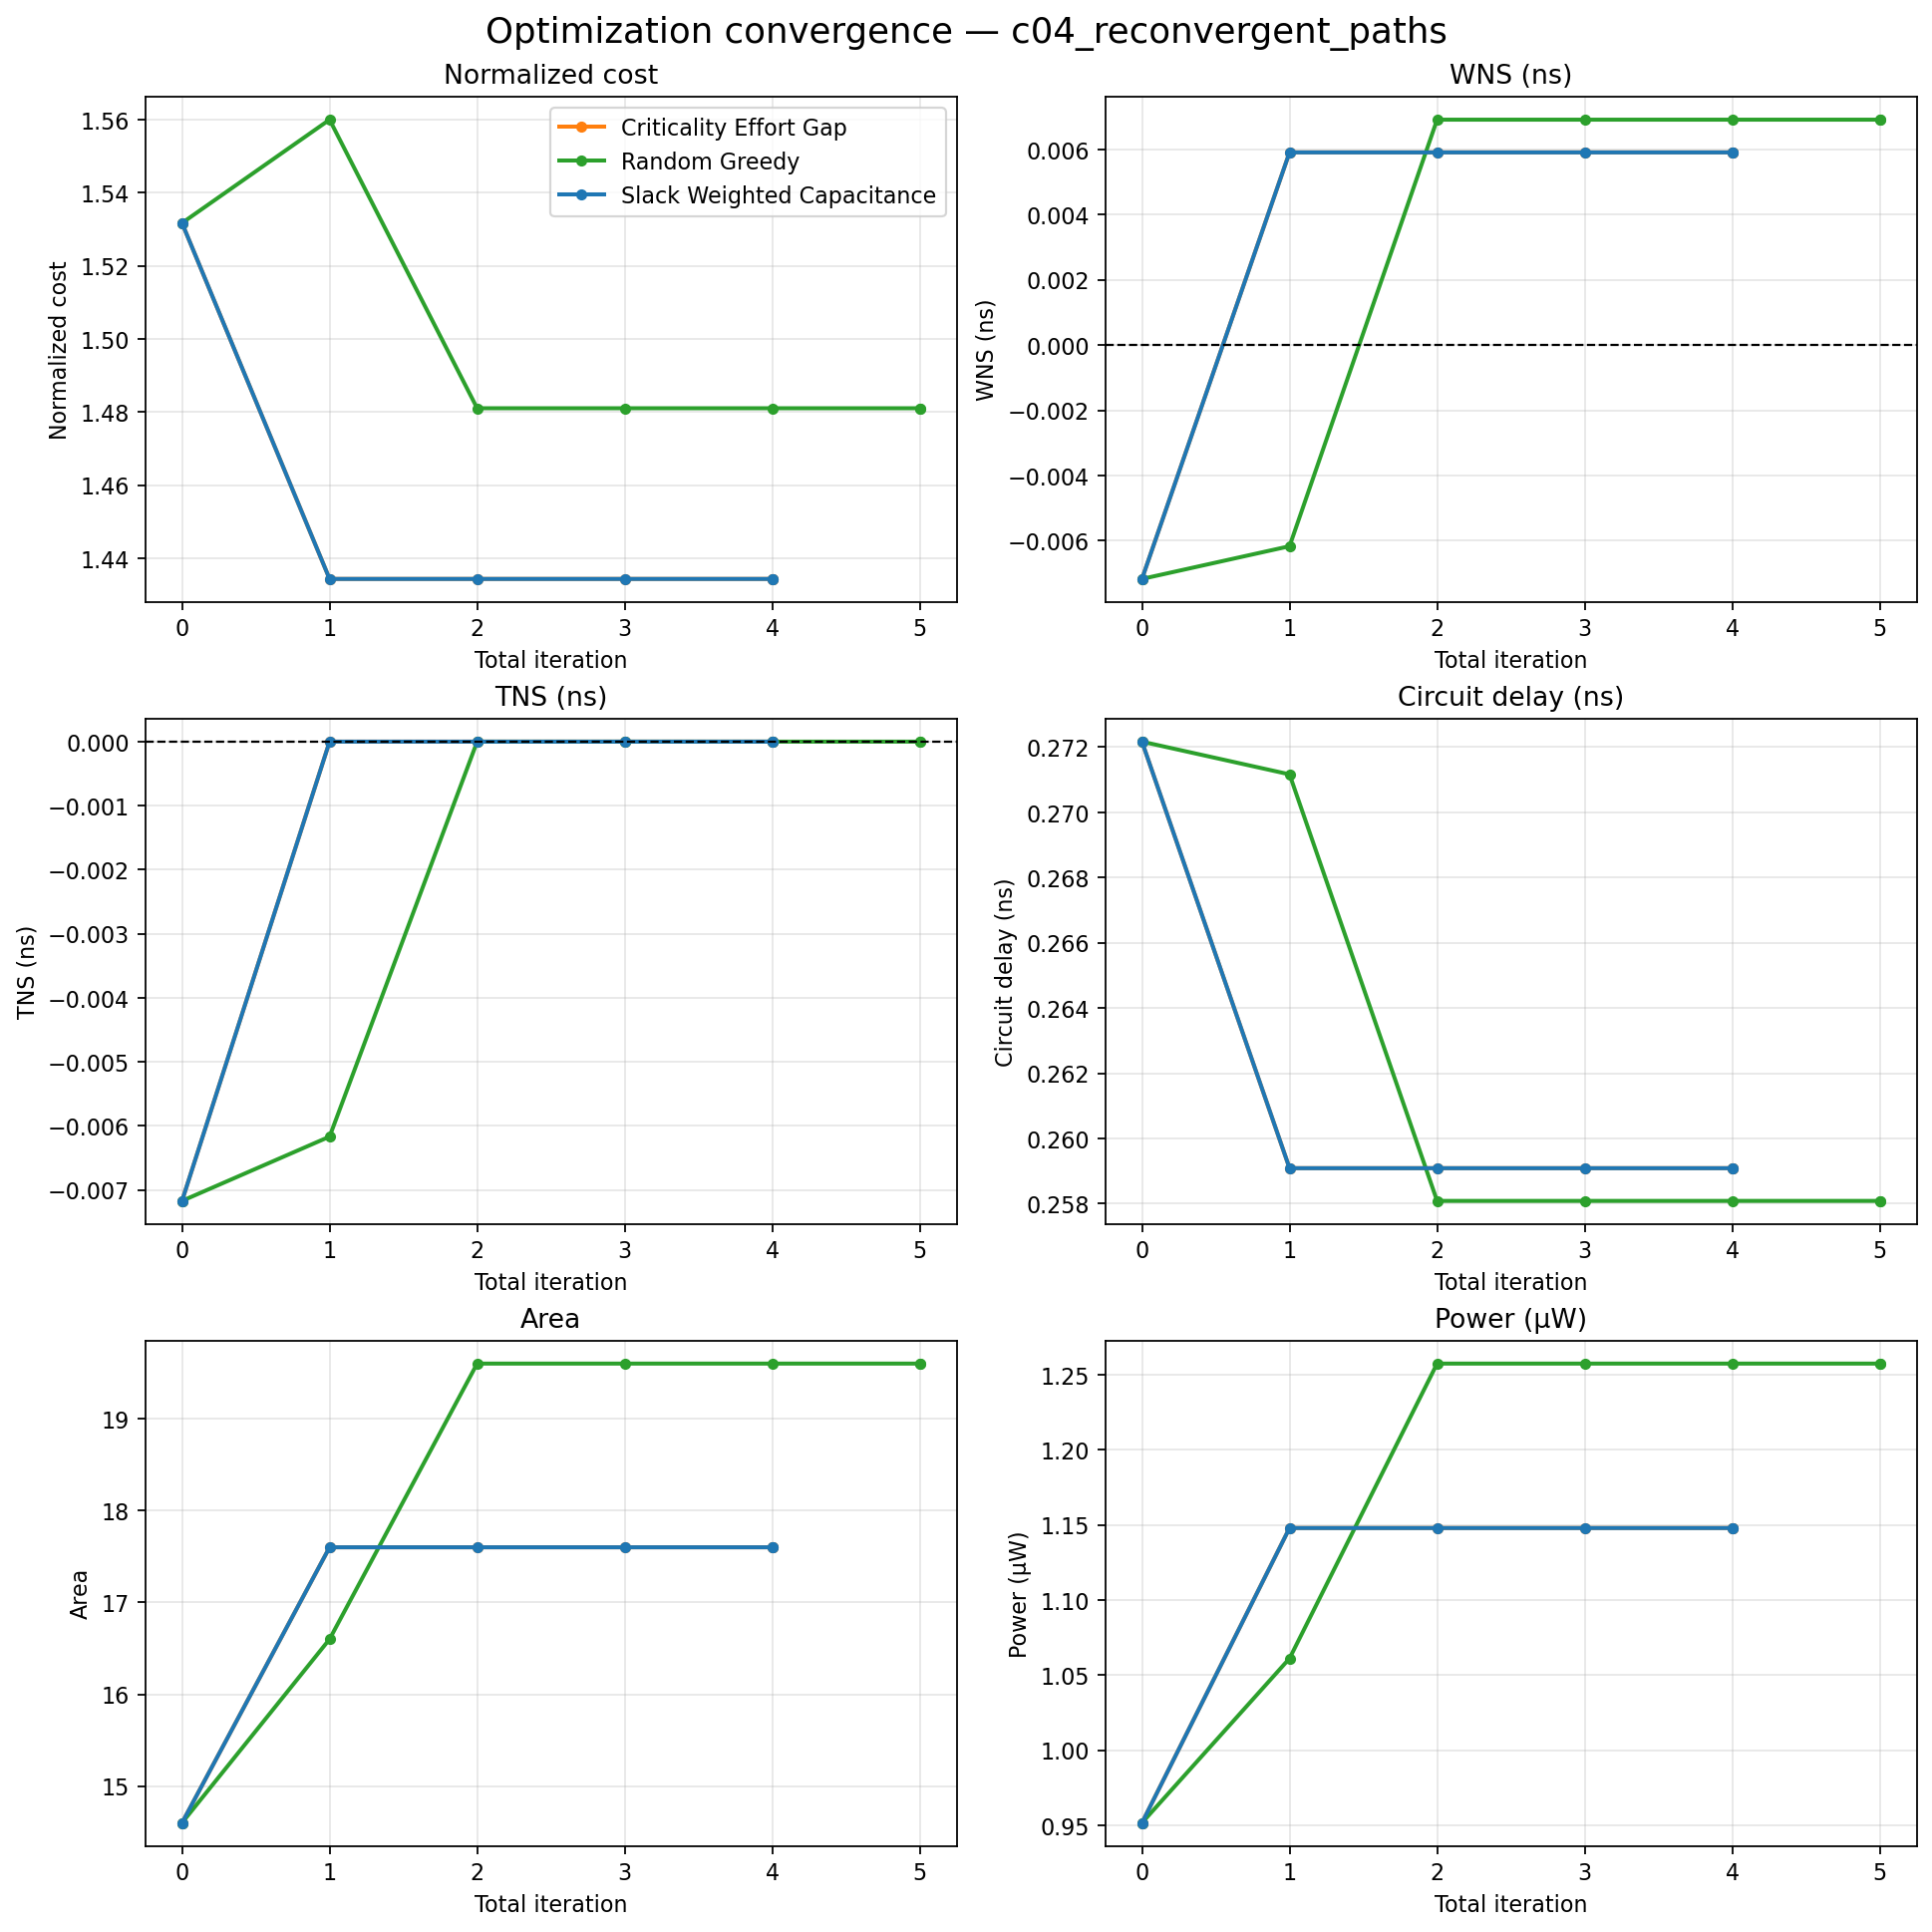
\includegraphics[width=\textwidth]{c04_reconvergent_paths_conv.png}
    \caption{\texttt{c04\_reconvergent\_paths}: optimization convergence trace.}
    \label{fig:app-c04-reconvergent-paths-conv}
\end{figure}

\begin{figure}[H]
    \centering
    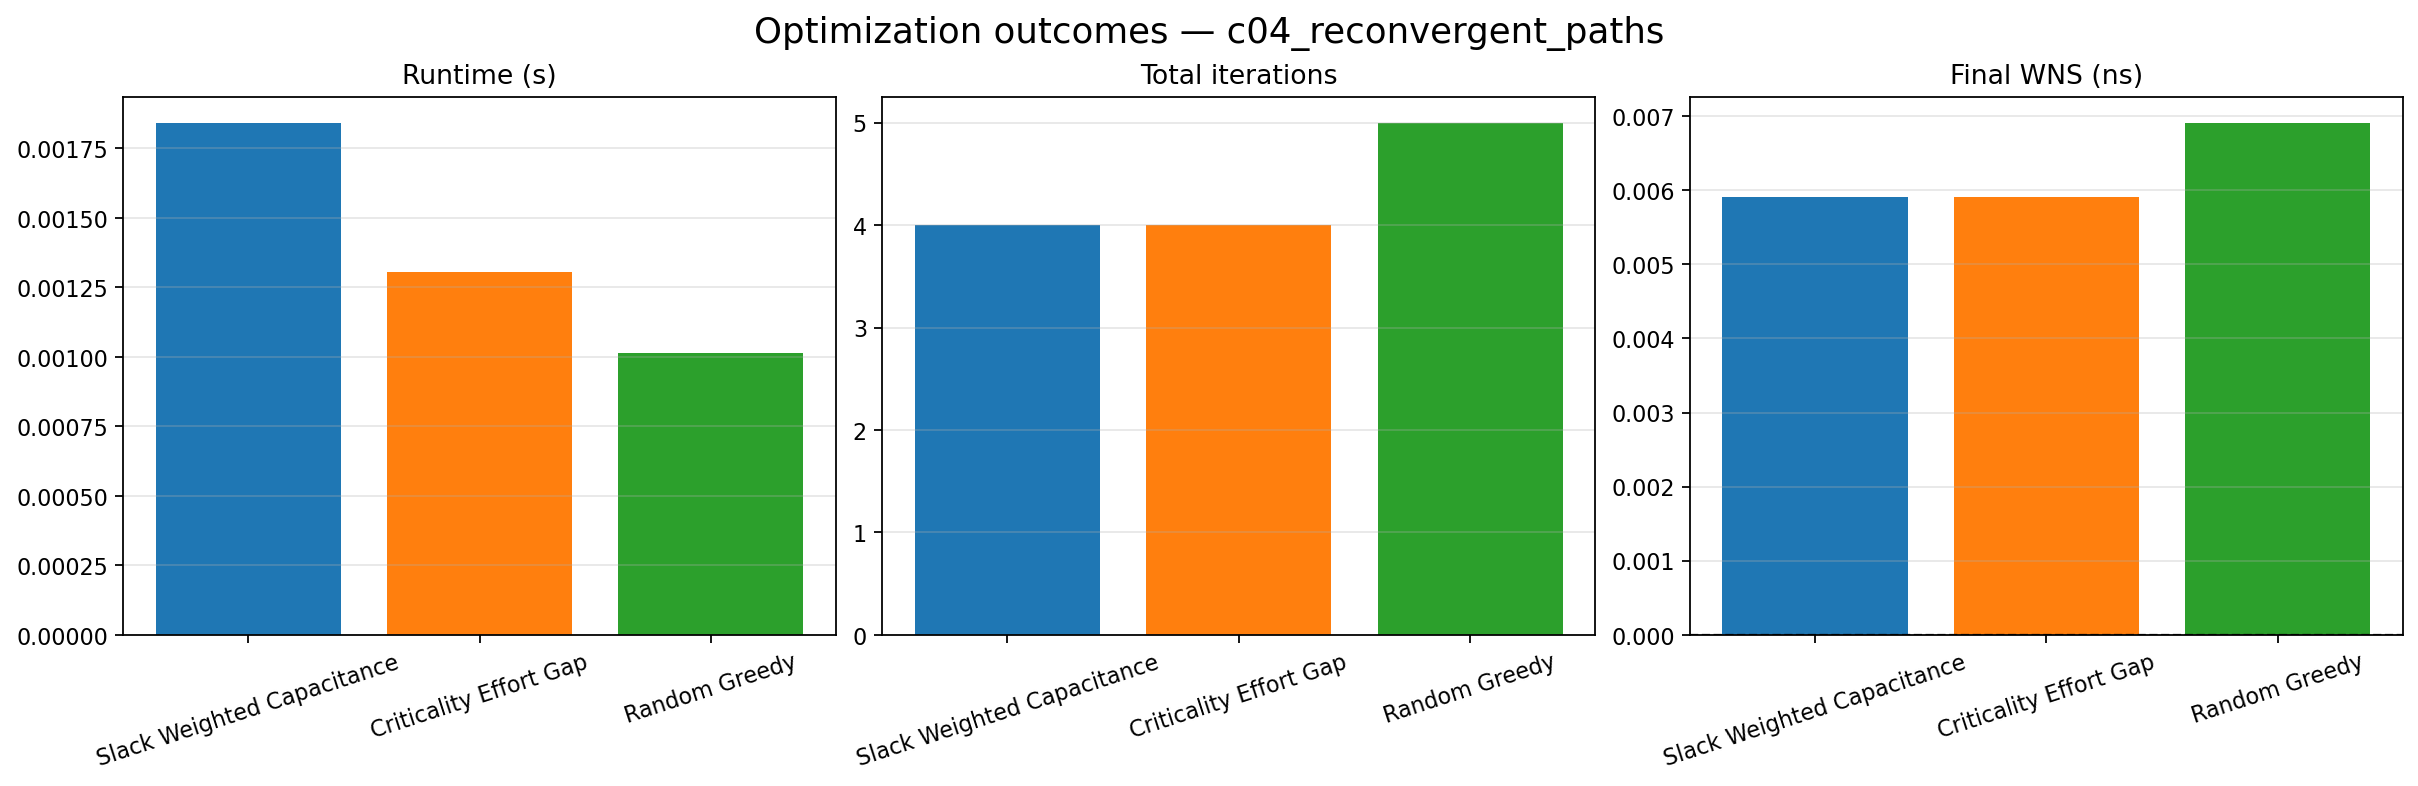
\includegraphics[width=\textwidth]{c04_reconvergent_paths_outc.png}
    \caption{\texttt{c04\_reconvergent\_paths}: optimization outcomes summary.}
    \label{fig:app-c04-reconvergent-paths-outc}
\end{figure}

\clearpage

\section{\texttt{c05\_multi\_output} (5 gates)}
\label{app:fig-c05-multi-output}

\begin{figure}[H]
    \centering
    \begin{subfigure}[t]{0.48\textwidth}
        \centering
        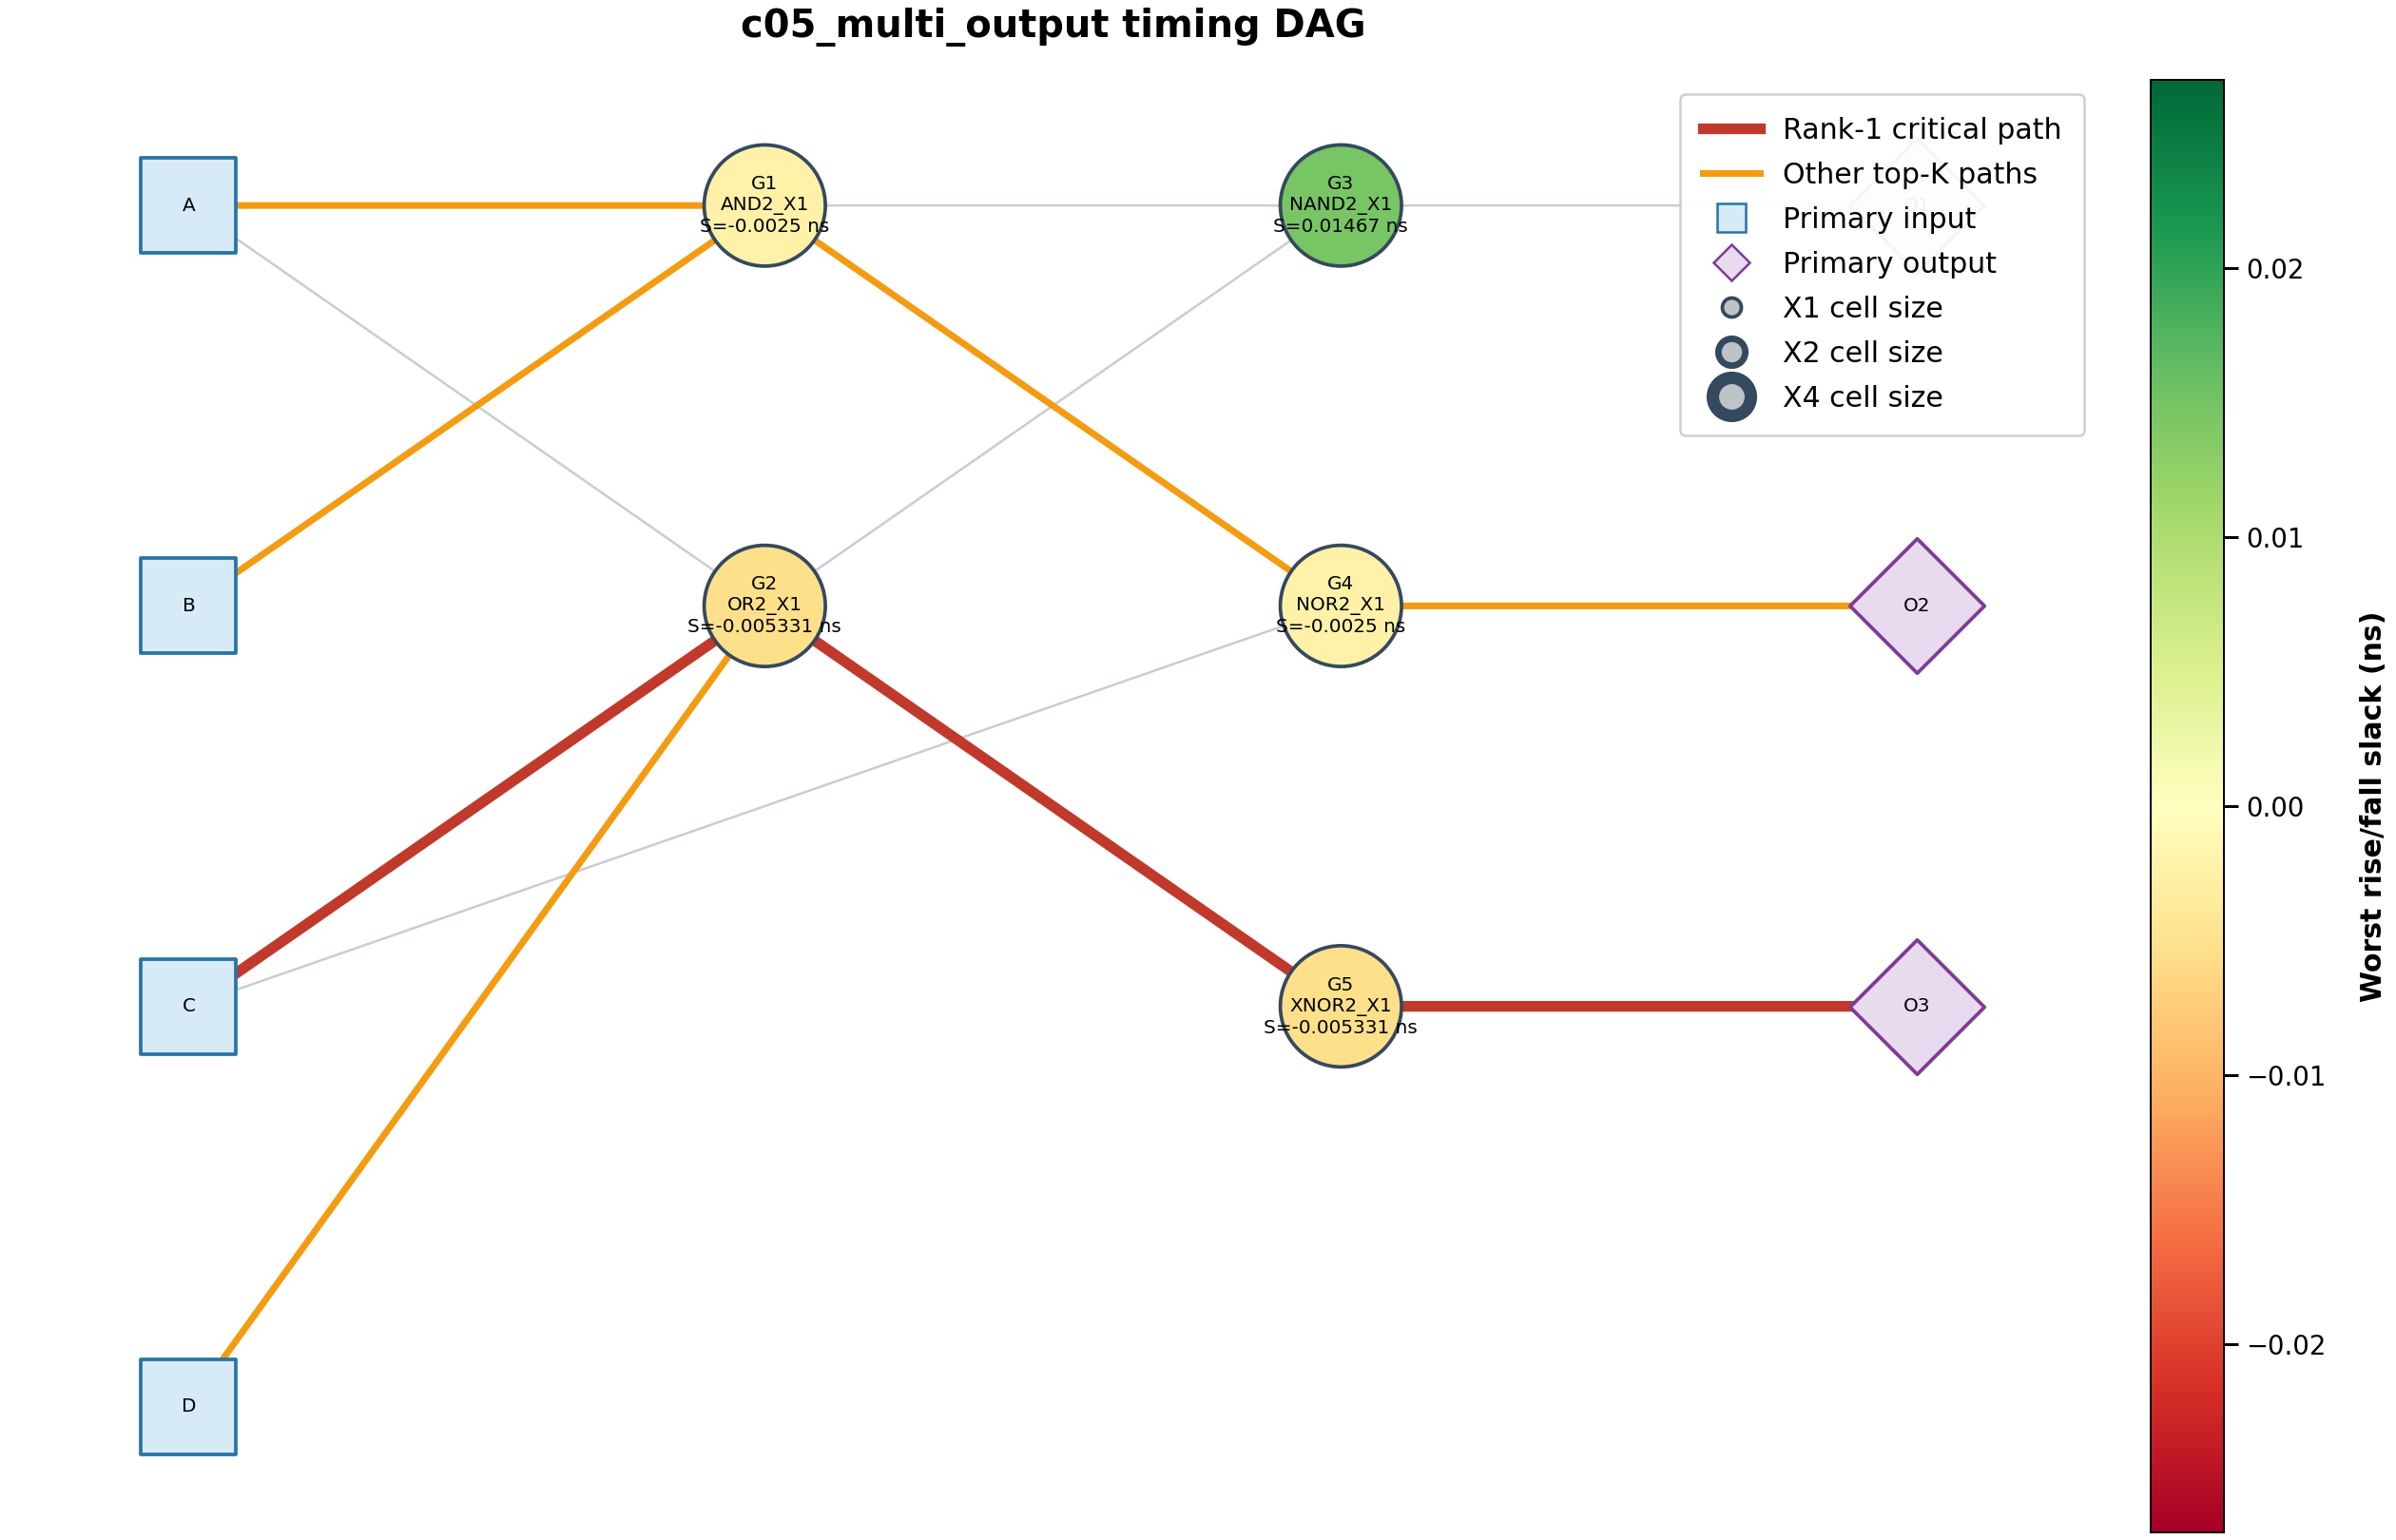
\includegraphics[width=\textwidth]{c05_multi_output_pre.png}
        \caption{Pre-optimization}
    \end{subfigure}
    \hfill
    \begin{subfigure}[t]{0.48\textwidth}
        \centering
        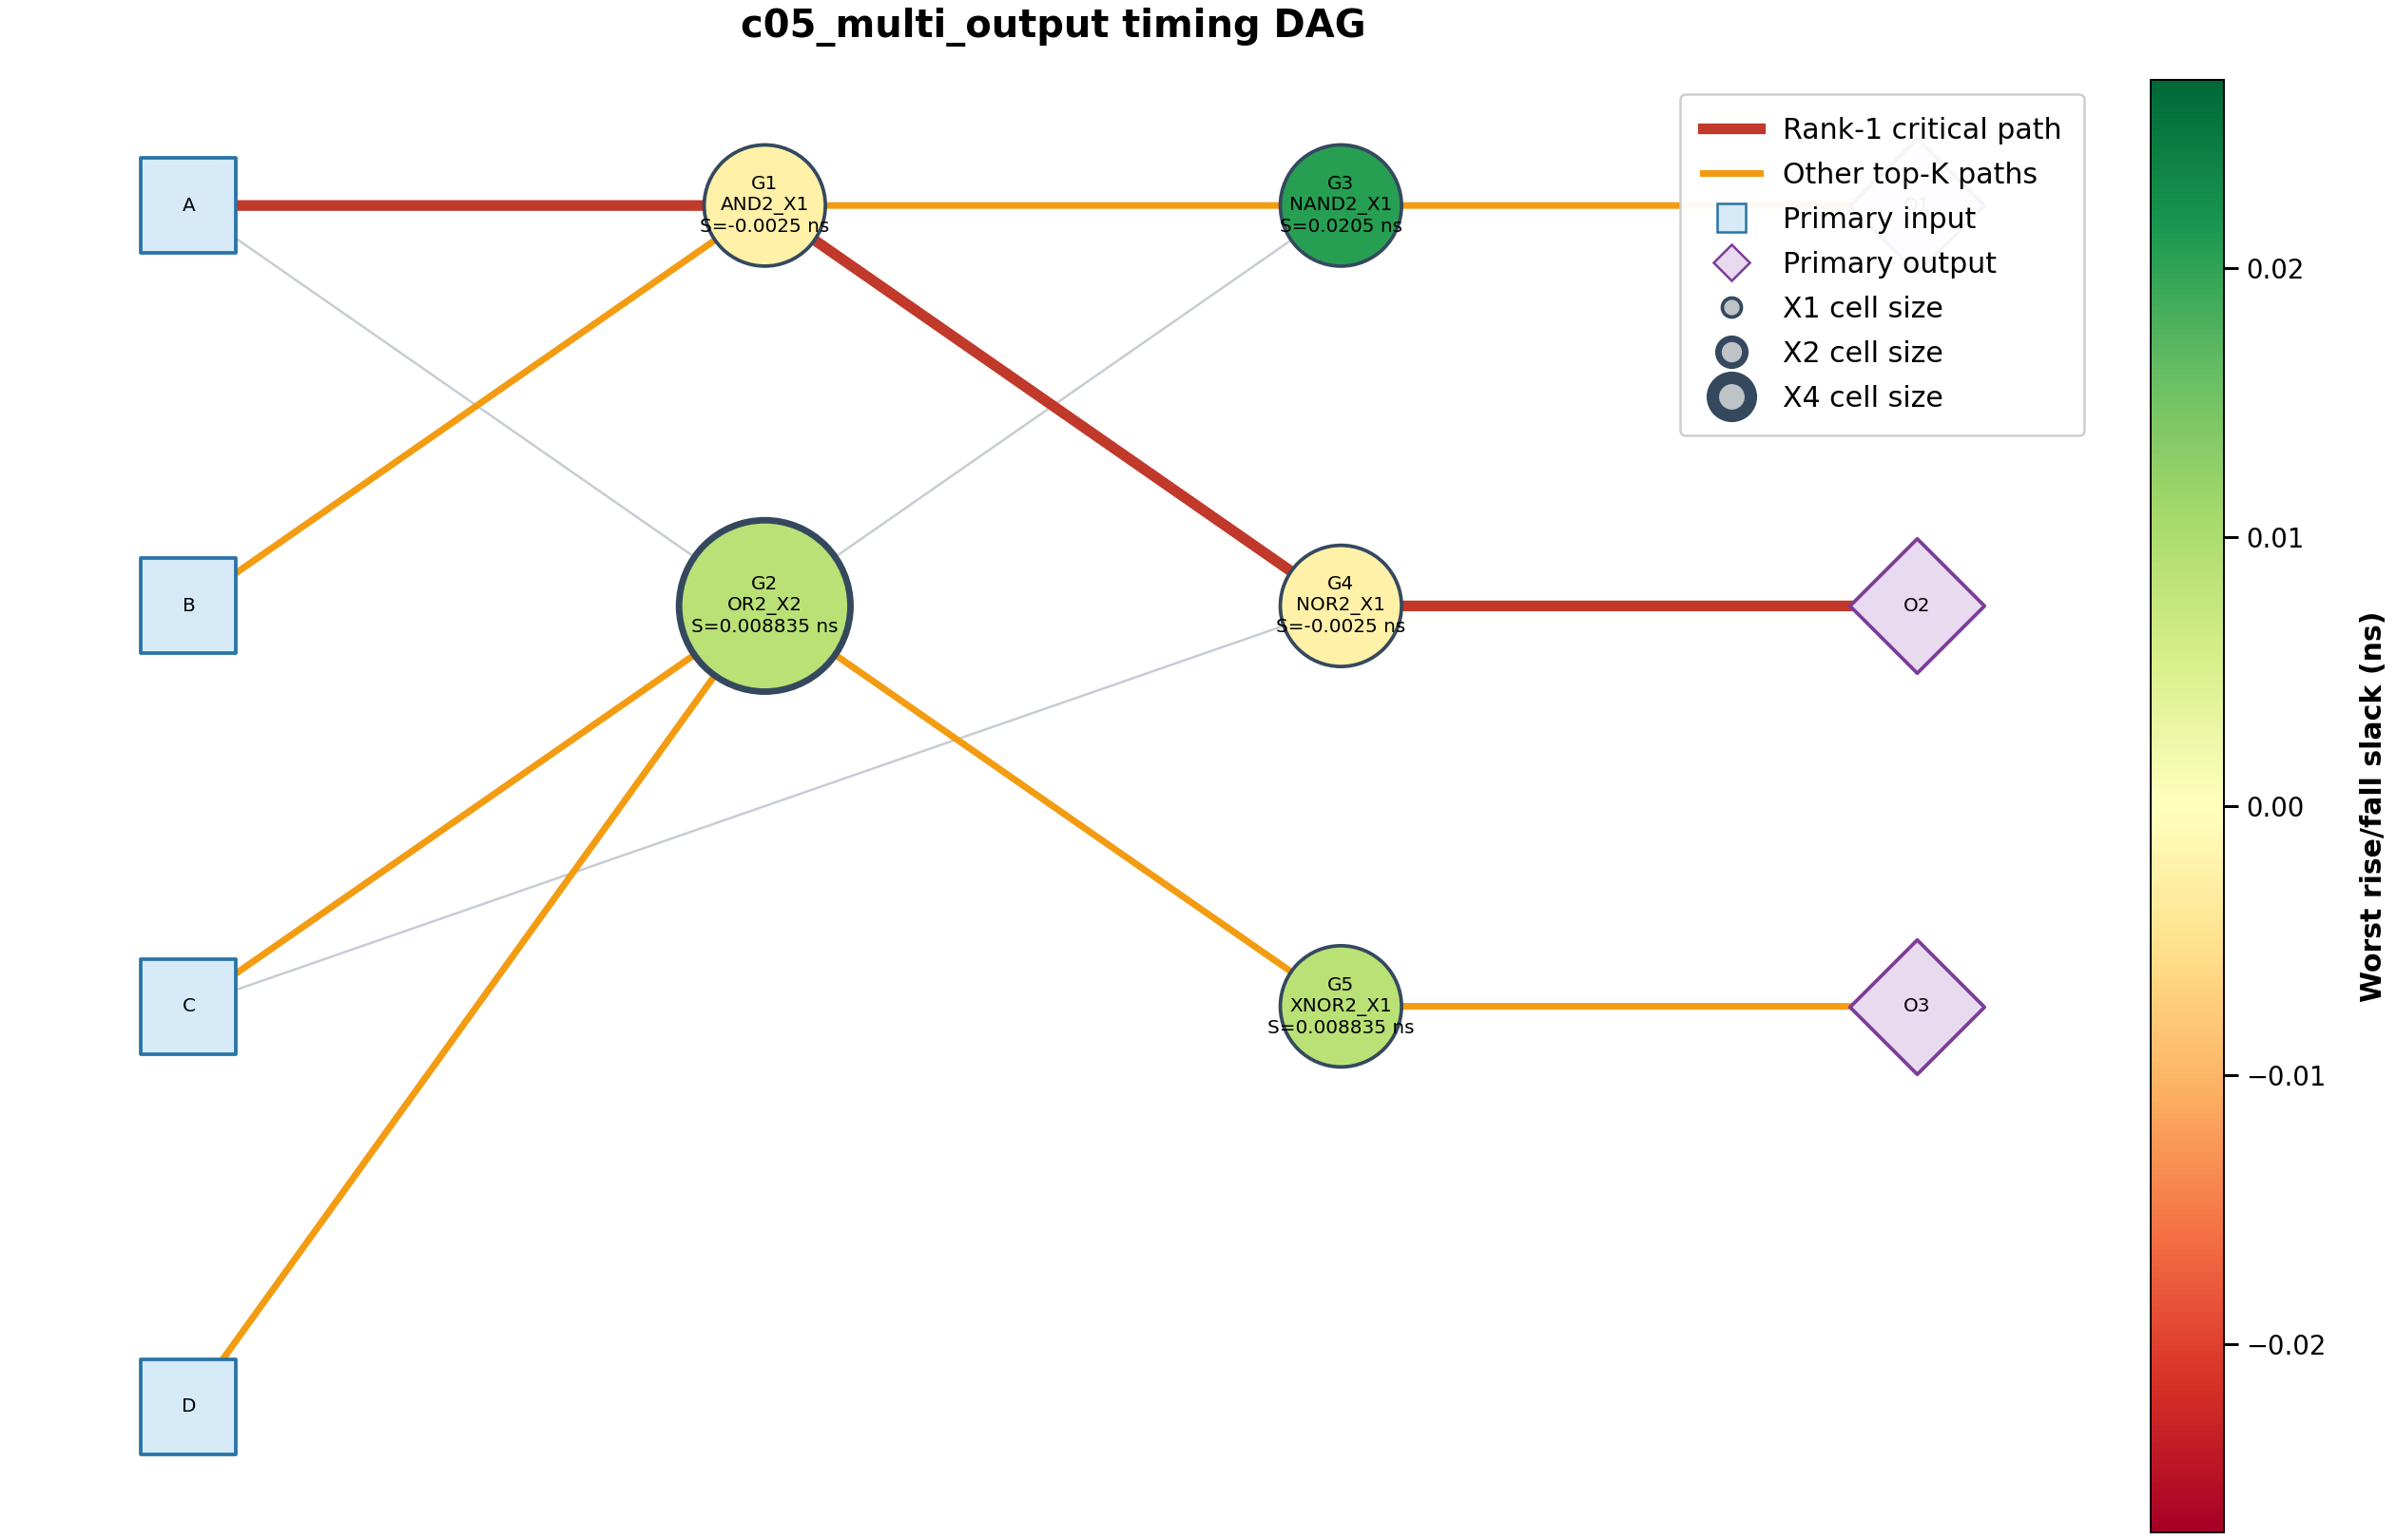
\includegraphics[width=\textwidth]{c05_multi_output_post.png}
        \caption{Post-optimization}
    \end{subfigure}
    \caption{\texttt{c05\_multi\_output}: circuit diagrams, nodes colored by slack,
    critical path highlighted.}
    \label{fig:app-c05-multi-output-graphs}
\end{figure}

\begin{figure}[H]
    \centering
    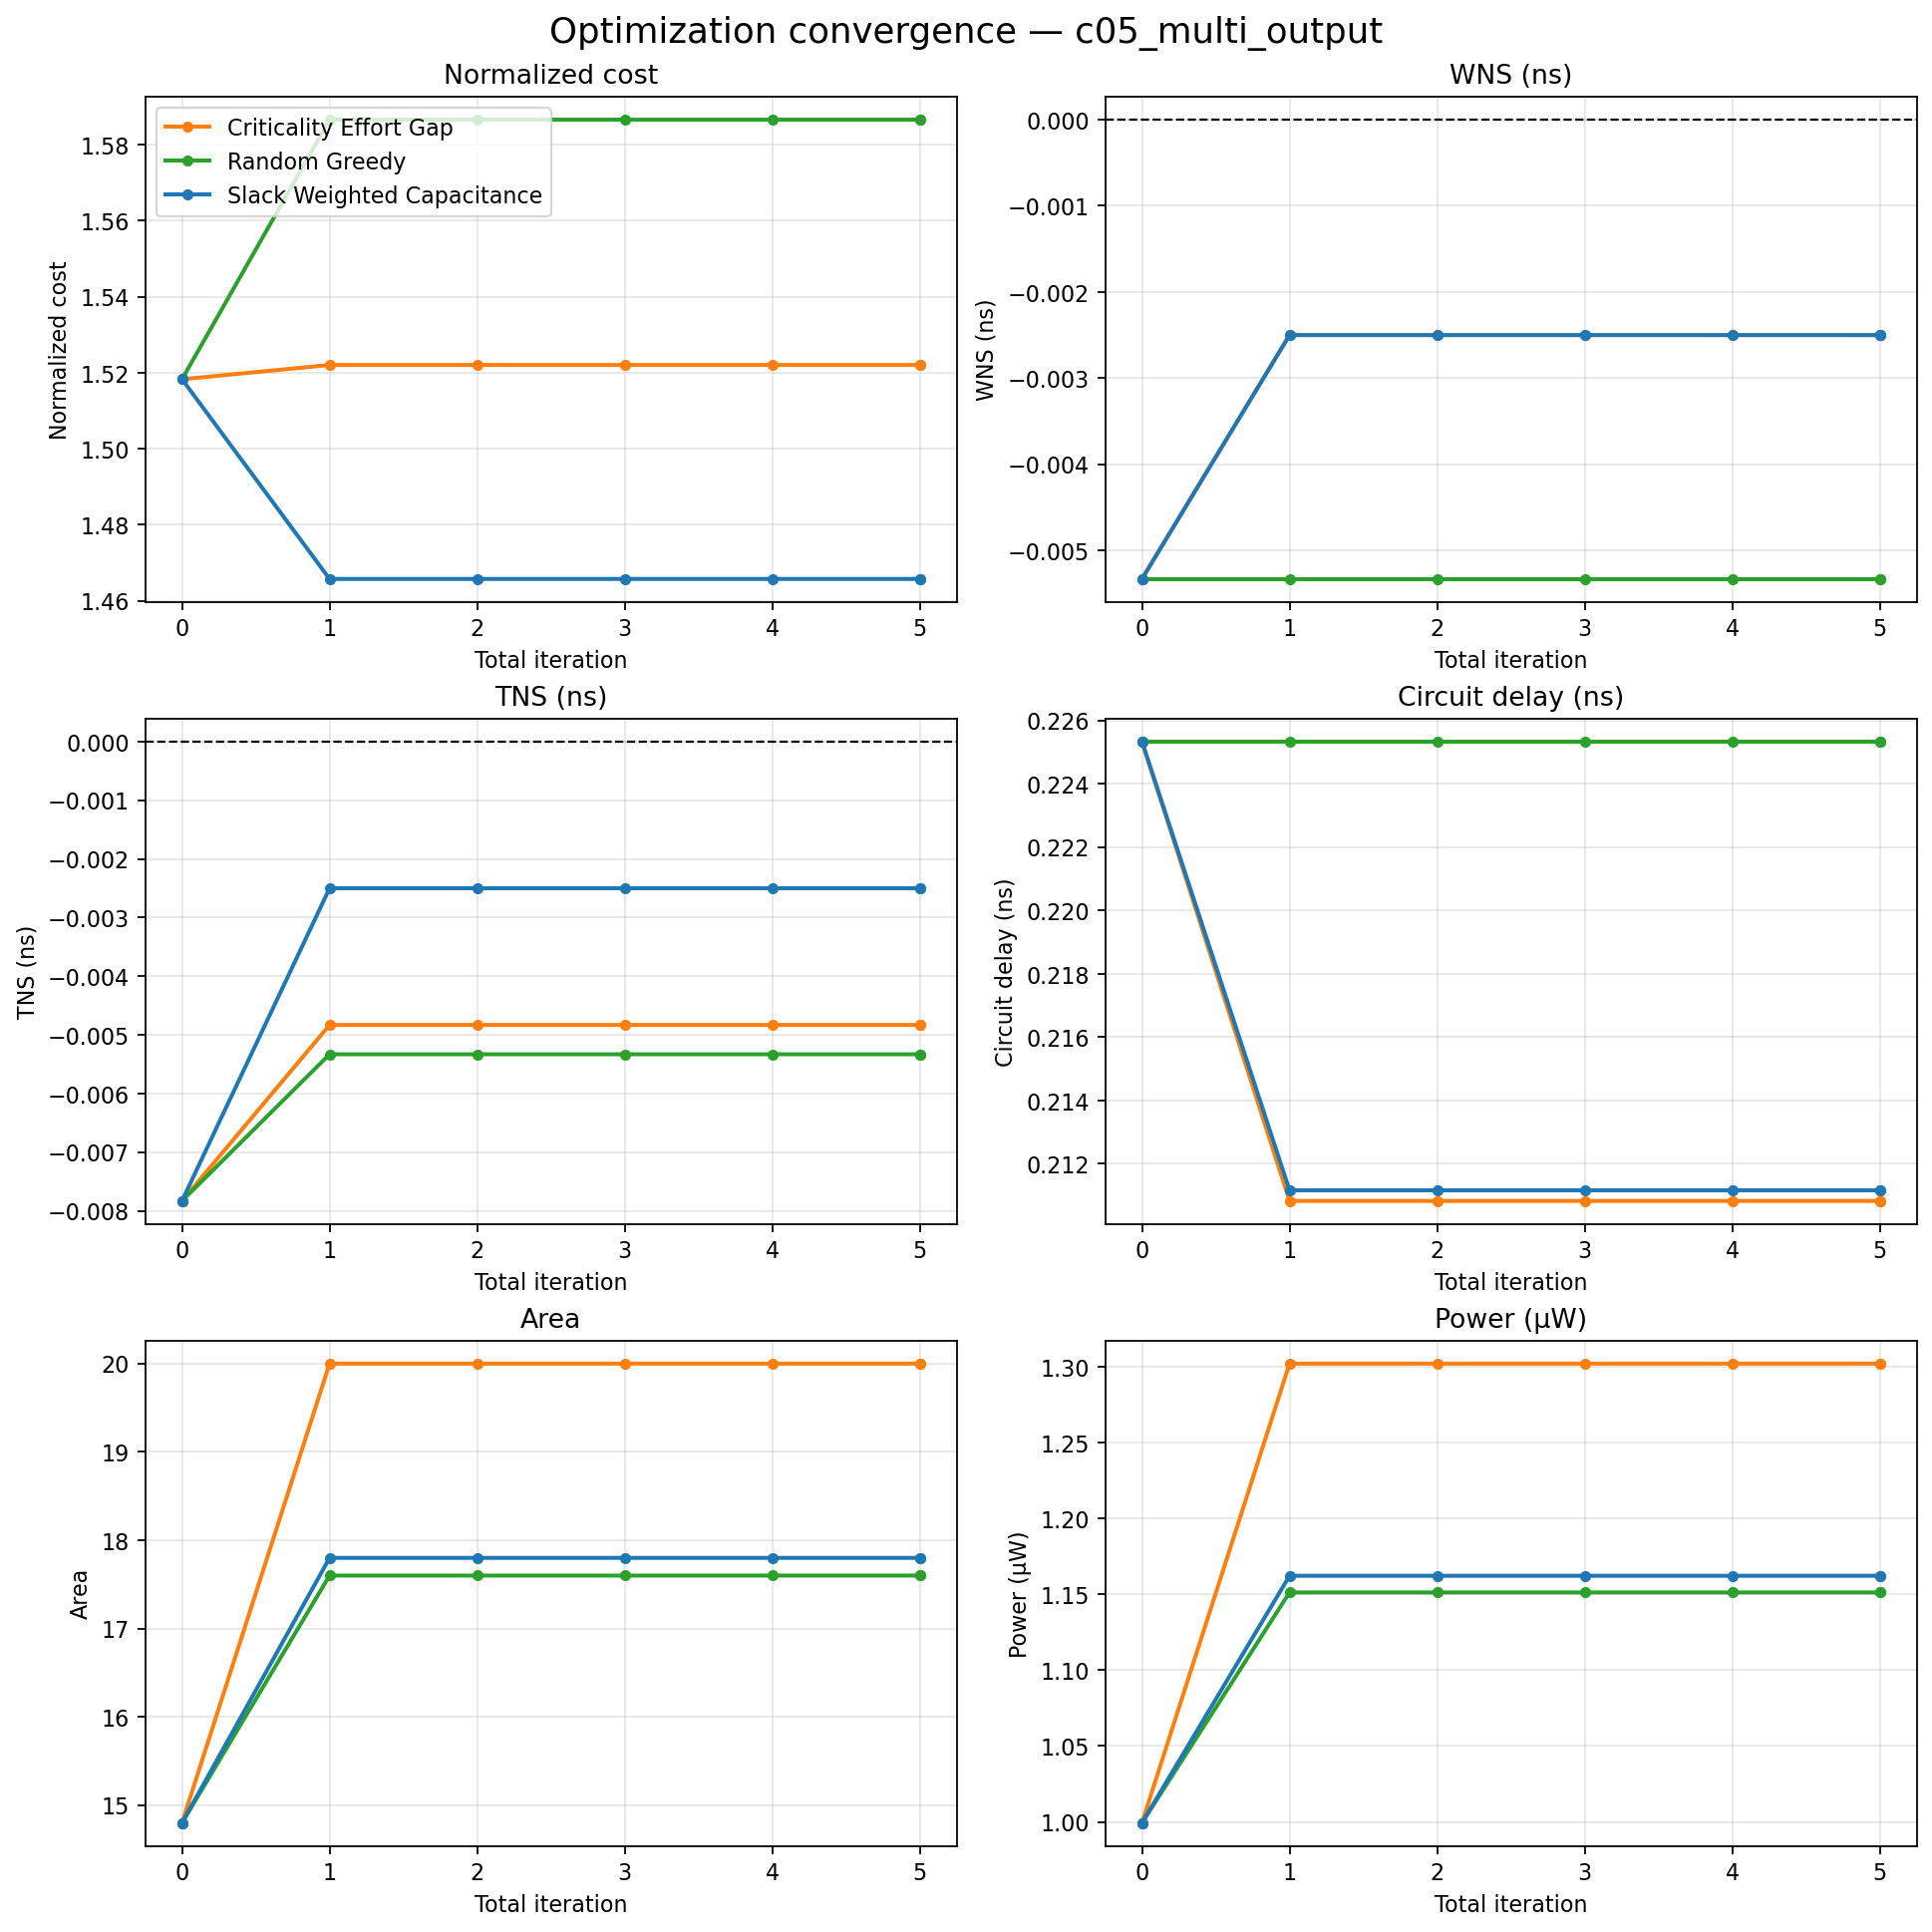
\includegraphics[width=\textwidth]{c05_multi_output_conv.png}
    \caption{\texttt{c05\_multi\_output}: optimization convergence trace.}
    \label{fig:app-c05-multi-output-conv}
\end{figure}

\begin{figure}[H]
    \centering
    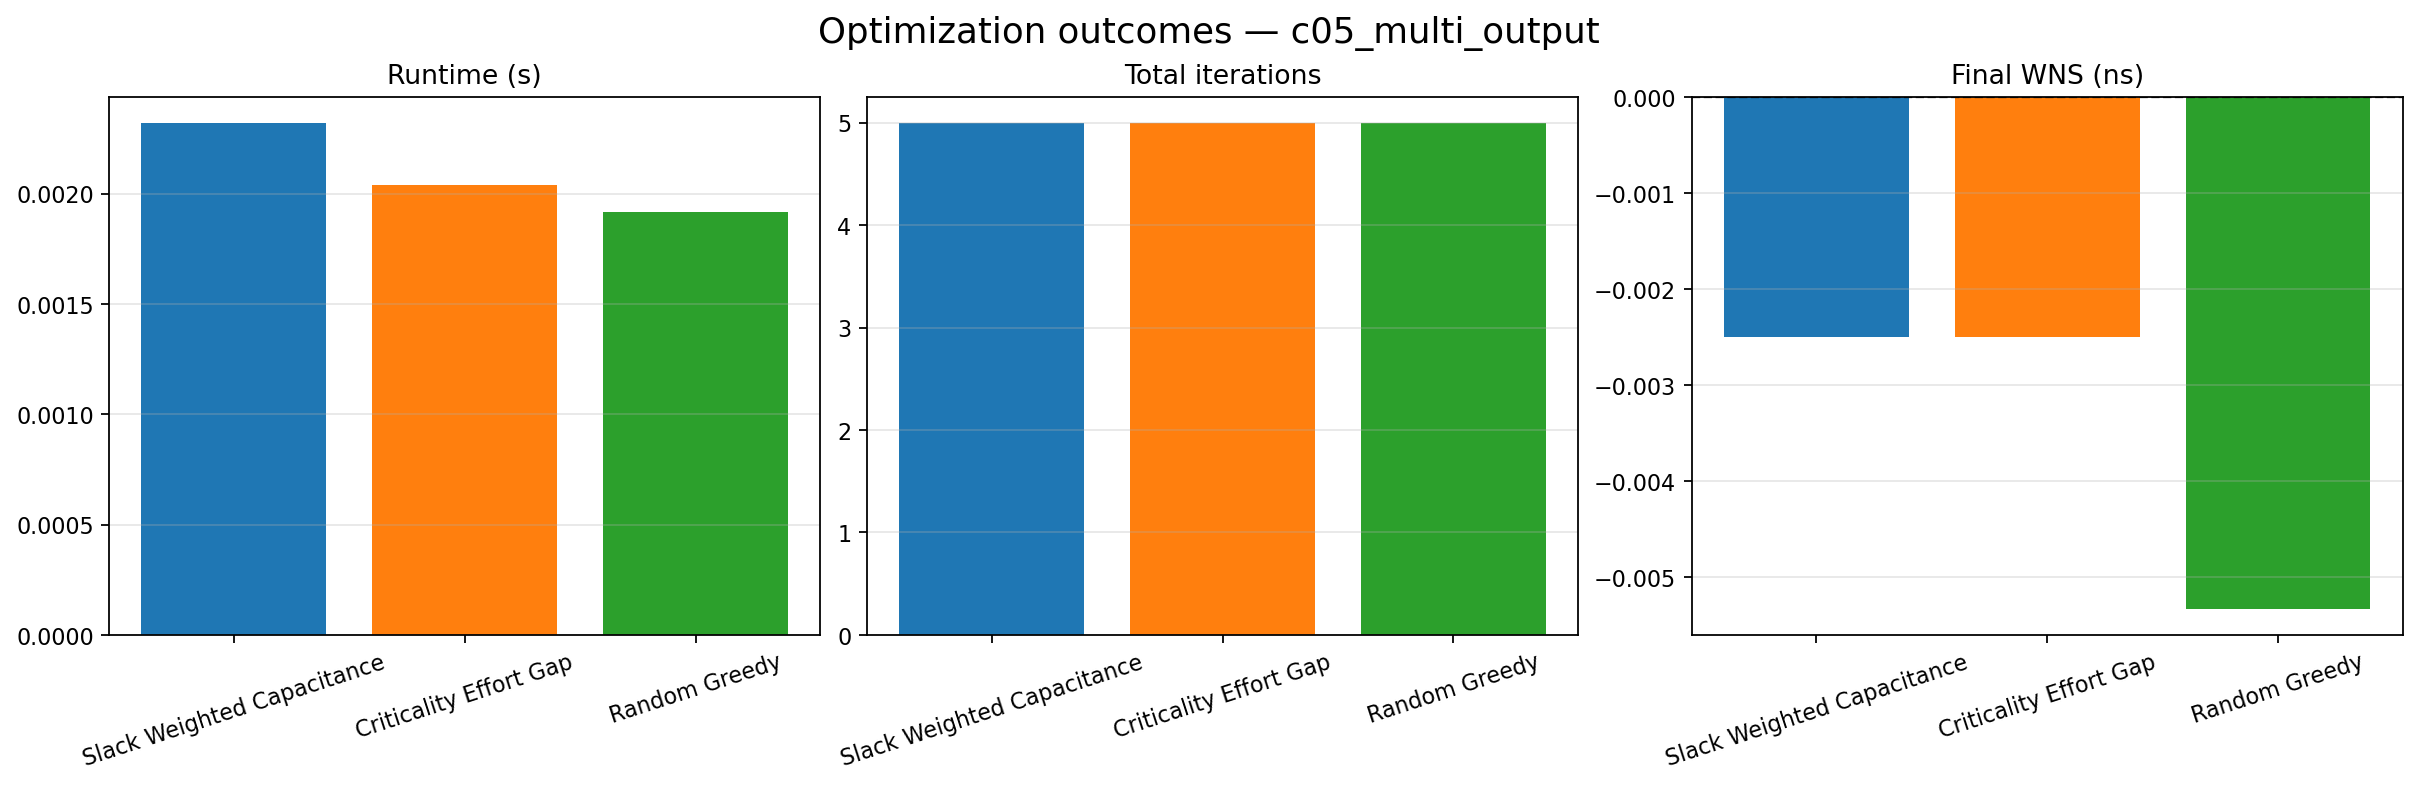
\includegraphics[width=\textwidth]{c05_multi_output_outc.png}
    \caption{\texttt{c05\_multi\_output}: optimization outcomes summary.}
    \label{fig:app-c05-multi-output-outc}
\end{figure}

\clearpage

\section{\texttt{c06\_deep\_critical\_path} (10 gates)}
\label{app:fig-c06-deep-critical-path}

\begin{figure}[H]
    \centering
    \begin{subfigure}[t]{0.48\textwidth}
        \centering
        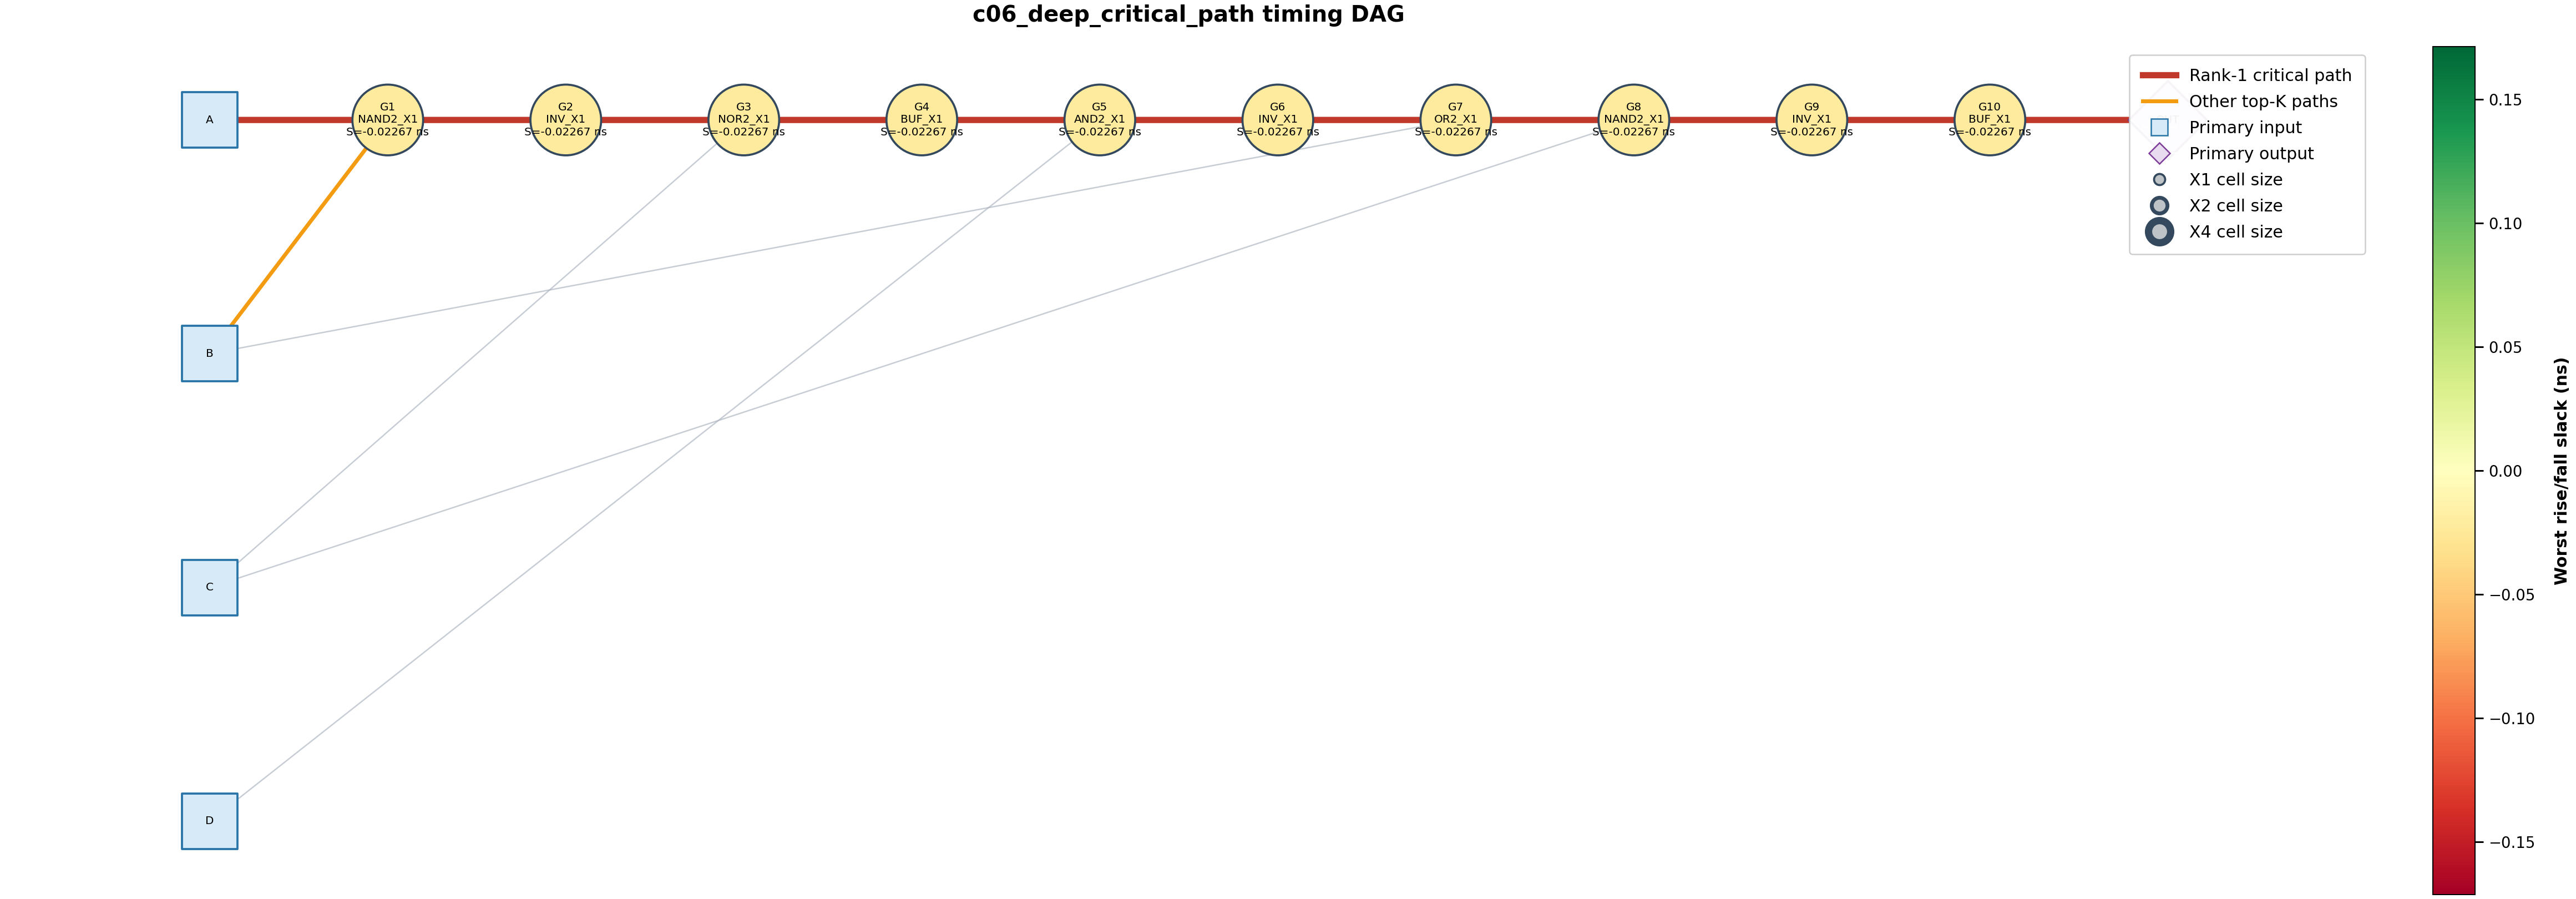
\includegraphics[width=\textwidth]{c06_deep_critical_path_pre.png}
        \caption{Pre-optimization}
    \end{subfigure}
    \hfill
    \begin{subfigure}[t]{0.48\textwidth}
        \centering
        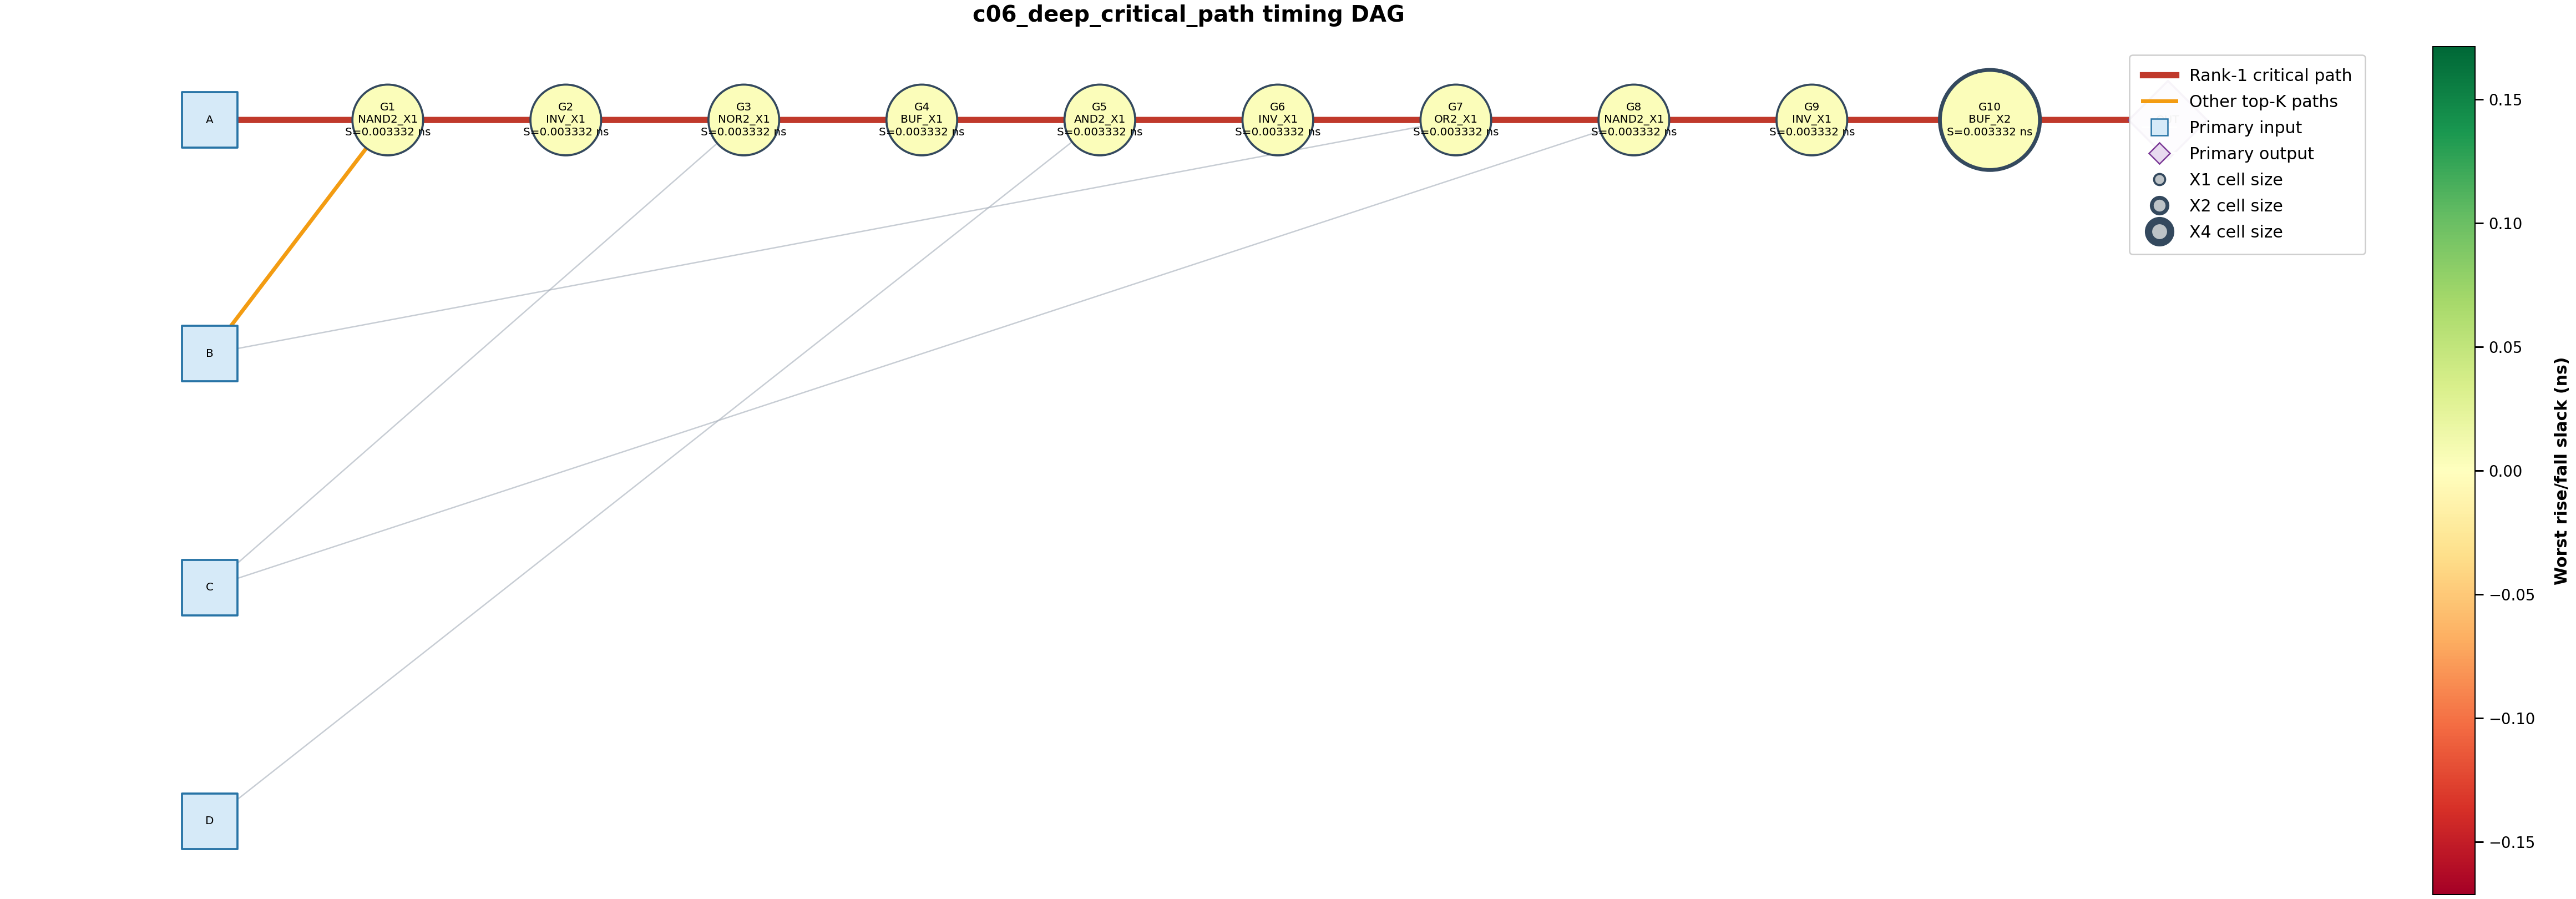
\includegraphics[width=\textwidth]{c06_deep_critical_path_post.png}
        \caption{Post-optimization}
    \end{subfigure}
    \caption{\texttt{c06\_deep\_critical\_path}: circuit diagrams, nodes colored by slack,
    critical path highlighted.}
    \label{fig:app-c06-deep-critical-path-graphs}
\end{figure}

\begin{figure}[H]
    \centering
    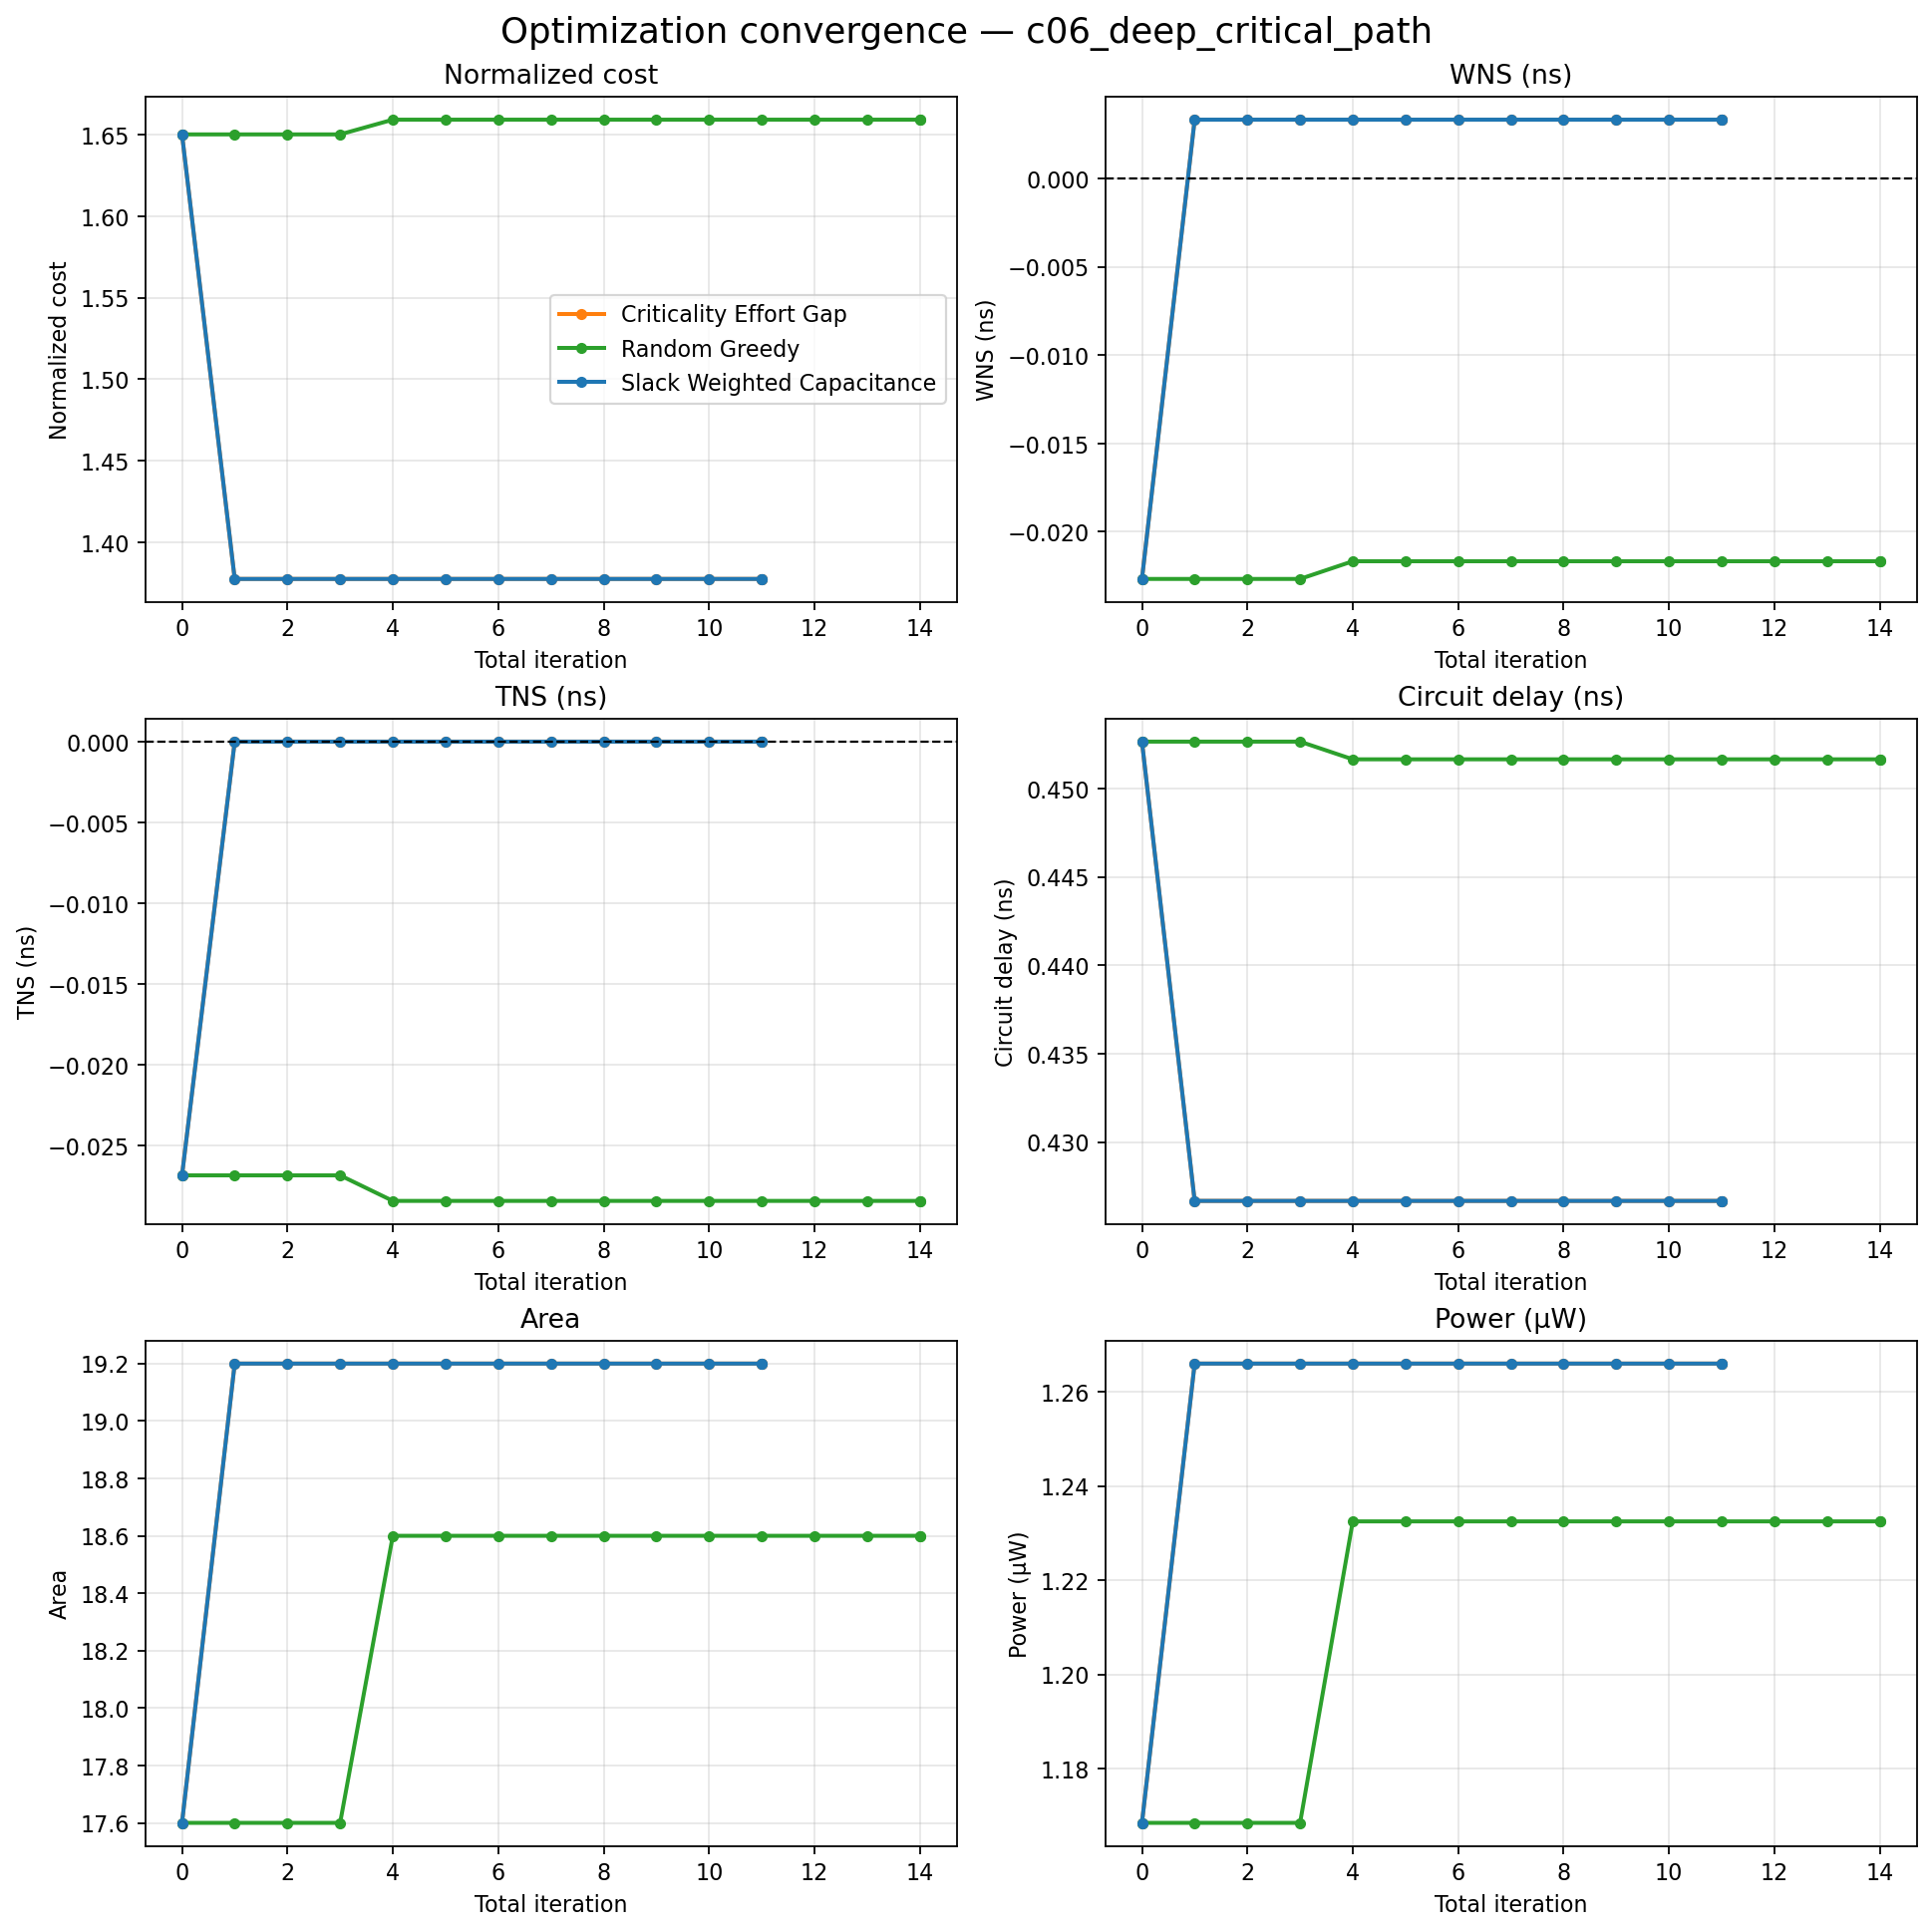
\includegraphics[width=\textwidth]{c06_deep_critical_path_conv.png}
    \caption{\texttt{c06\_deep\_critical\_path}: optimization convergence trace.}
    \label{fig:app-c06-deep-critical-path-conv}
\end{figure}

\begin{figure}[H]
    \centering
    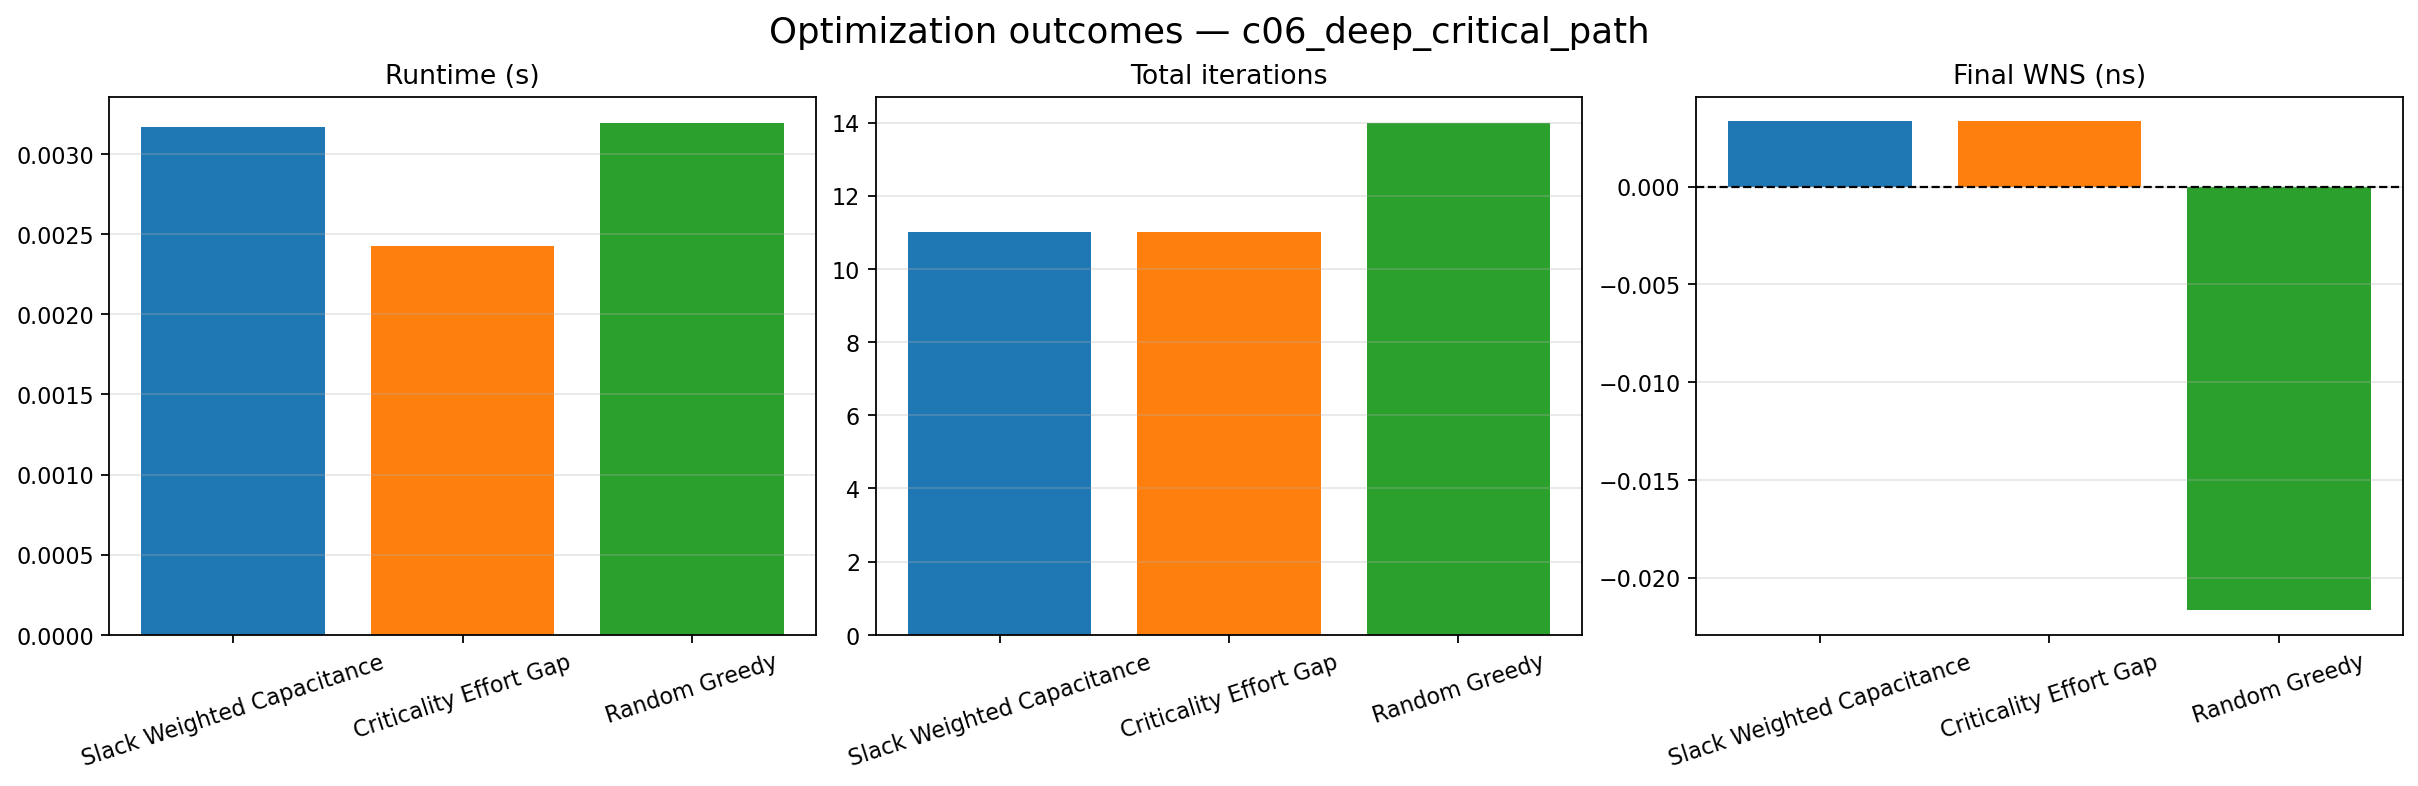
\includegraphics[width=\textwidth]{c06_deep_critical_path_outc.png}
    \caption{\texttt{c06\_deep\_critical\_path}: optimization outcomes summary.}
    \label{fig:app-c06-deep-critical-path-outc}
\end{figure}

\clearpage

\section{\texttt{c07\_parallel\_paths} (6 gates)}
\label{app:fig-c07-parallel-paths}

\begin{figure}[H]
    \centering
    \begin{subfigure}[t]{0.48\textwidth}
        \centering
        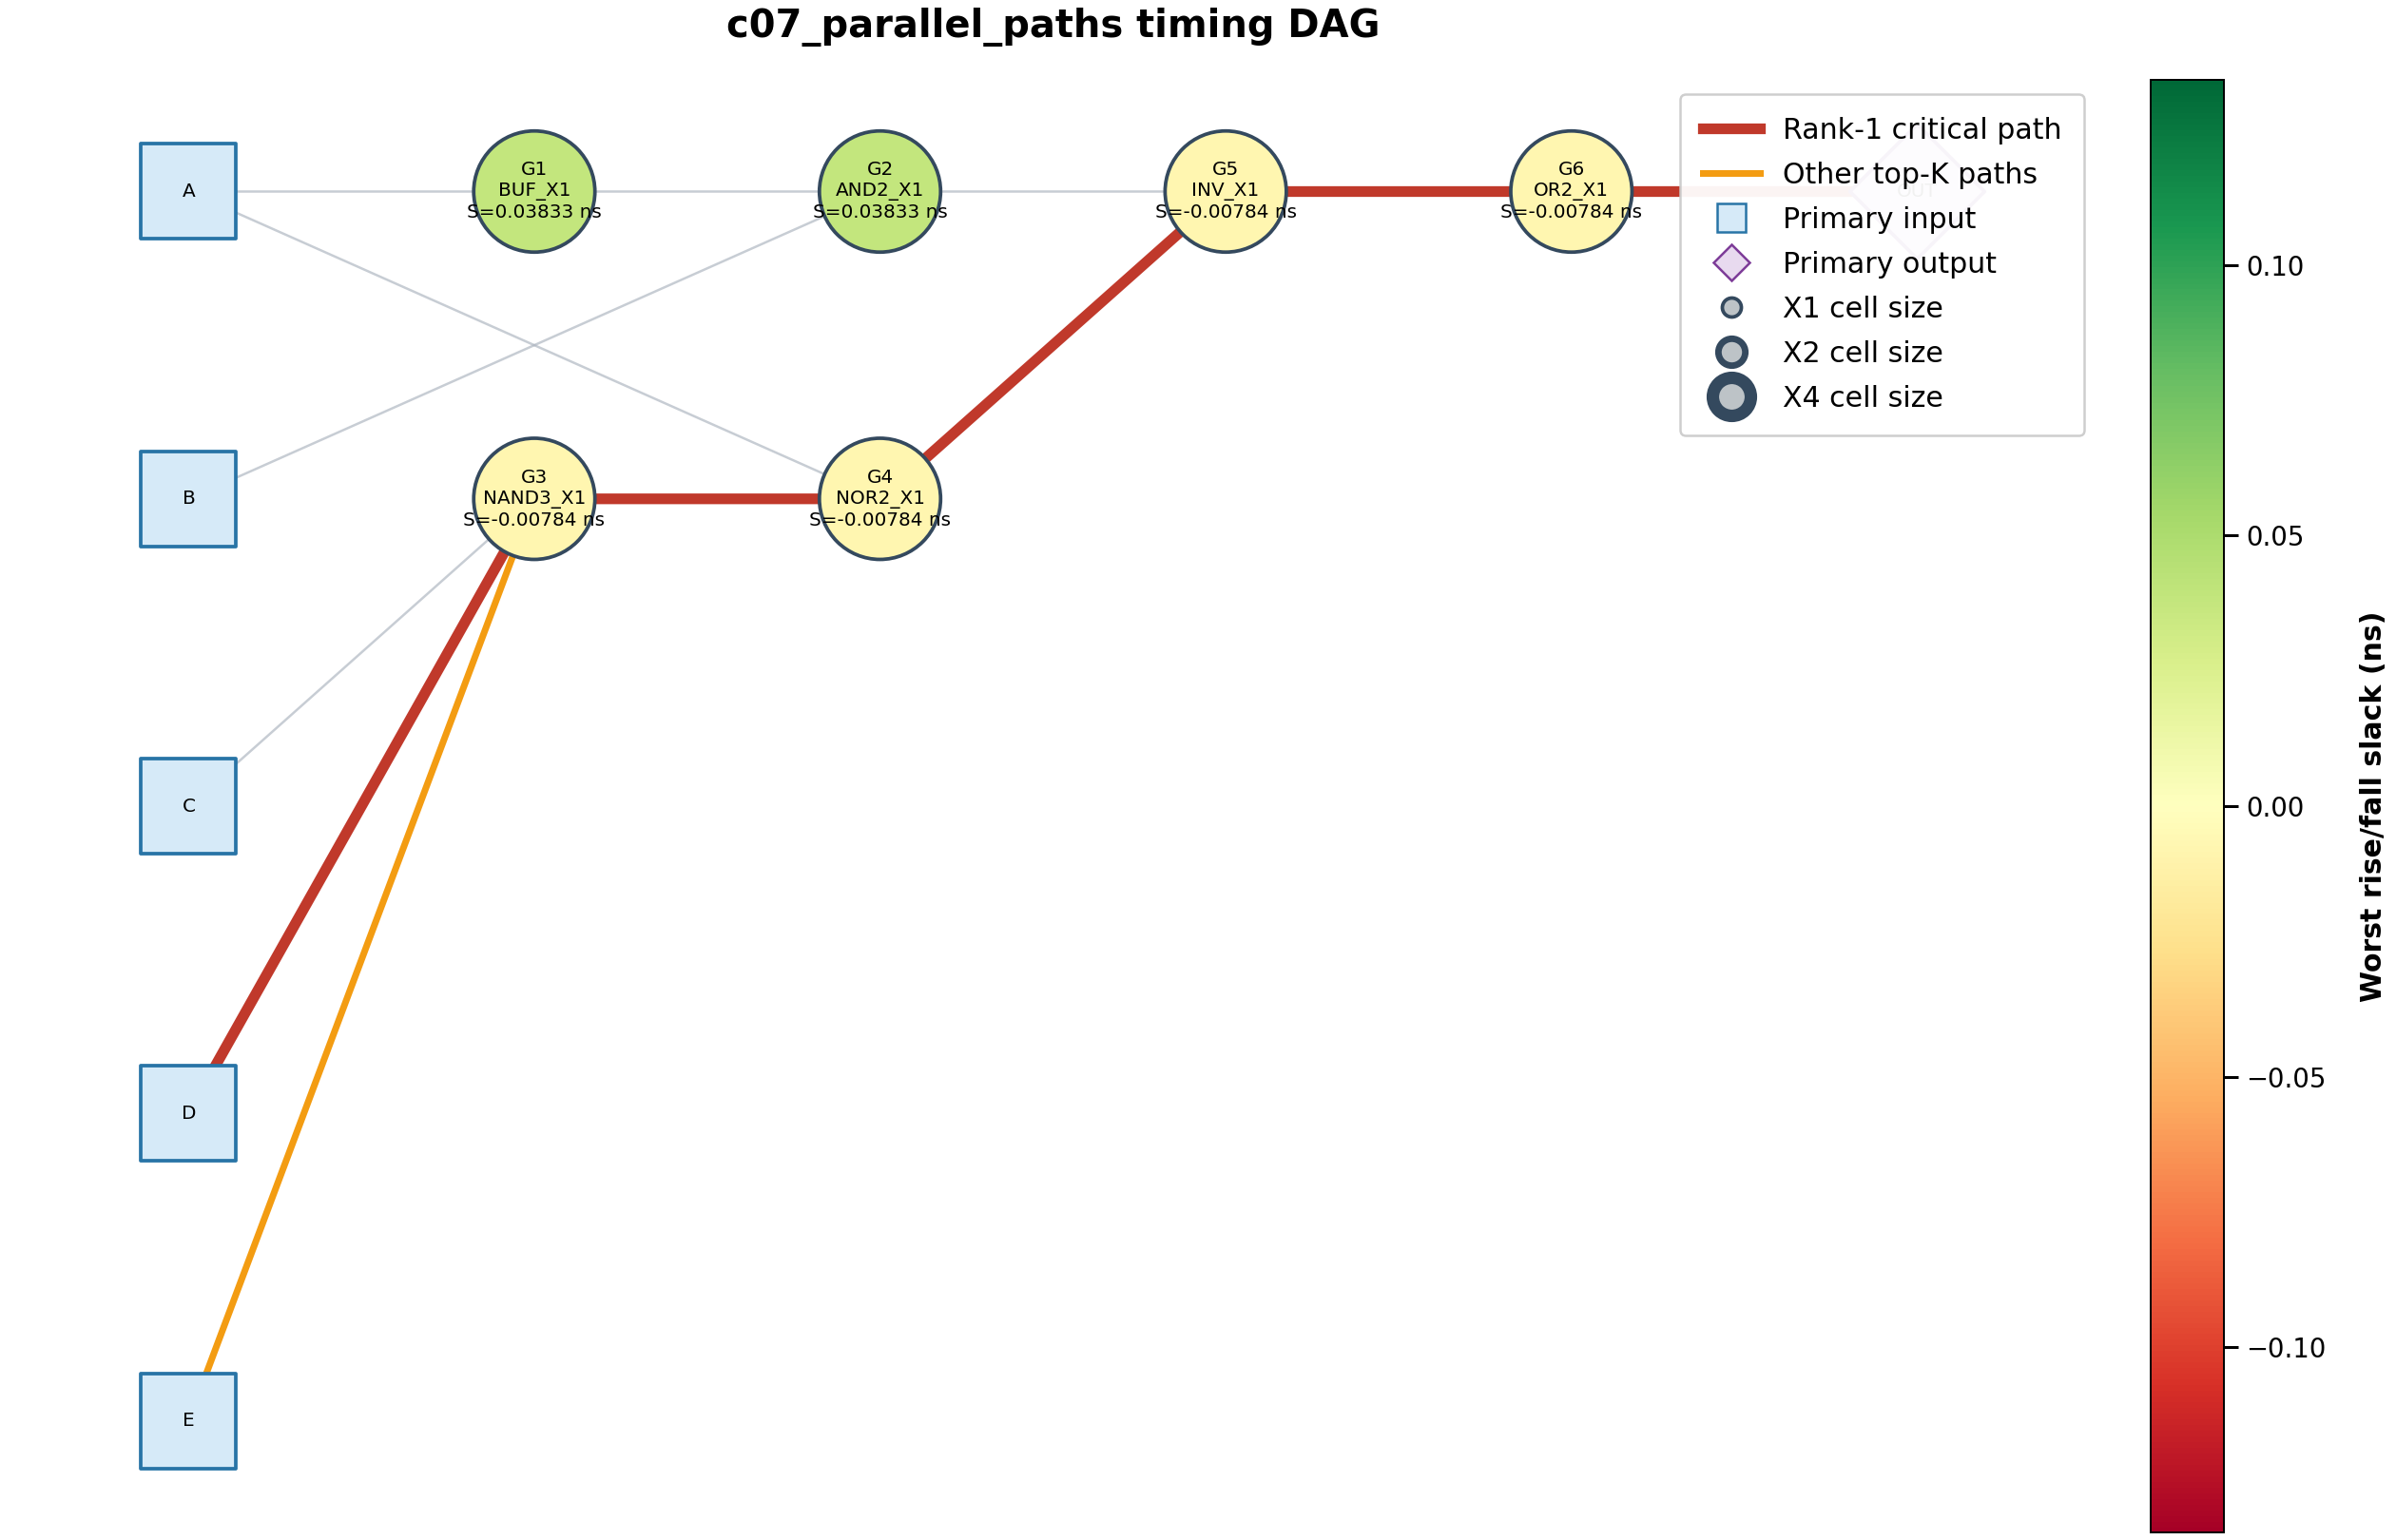
\includegraphics[width=\textwidth]{c07_parallel_paths_pre.png}
        \caption{Pre-optimization}
    \end{subfigure}
    \hfill
    \begin{subfigure}[t]{0.48\textwidth}
        \centering
        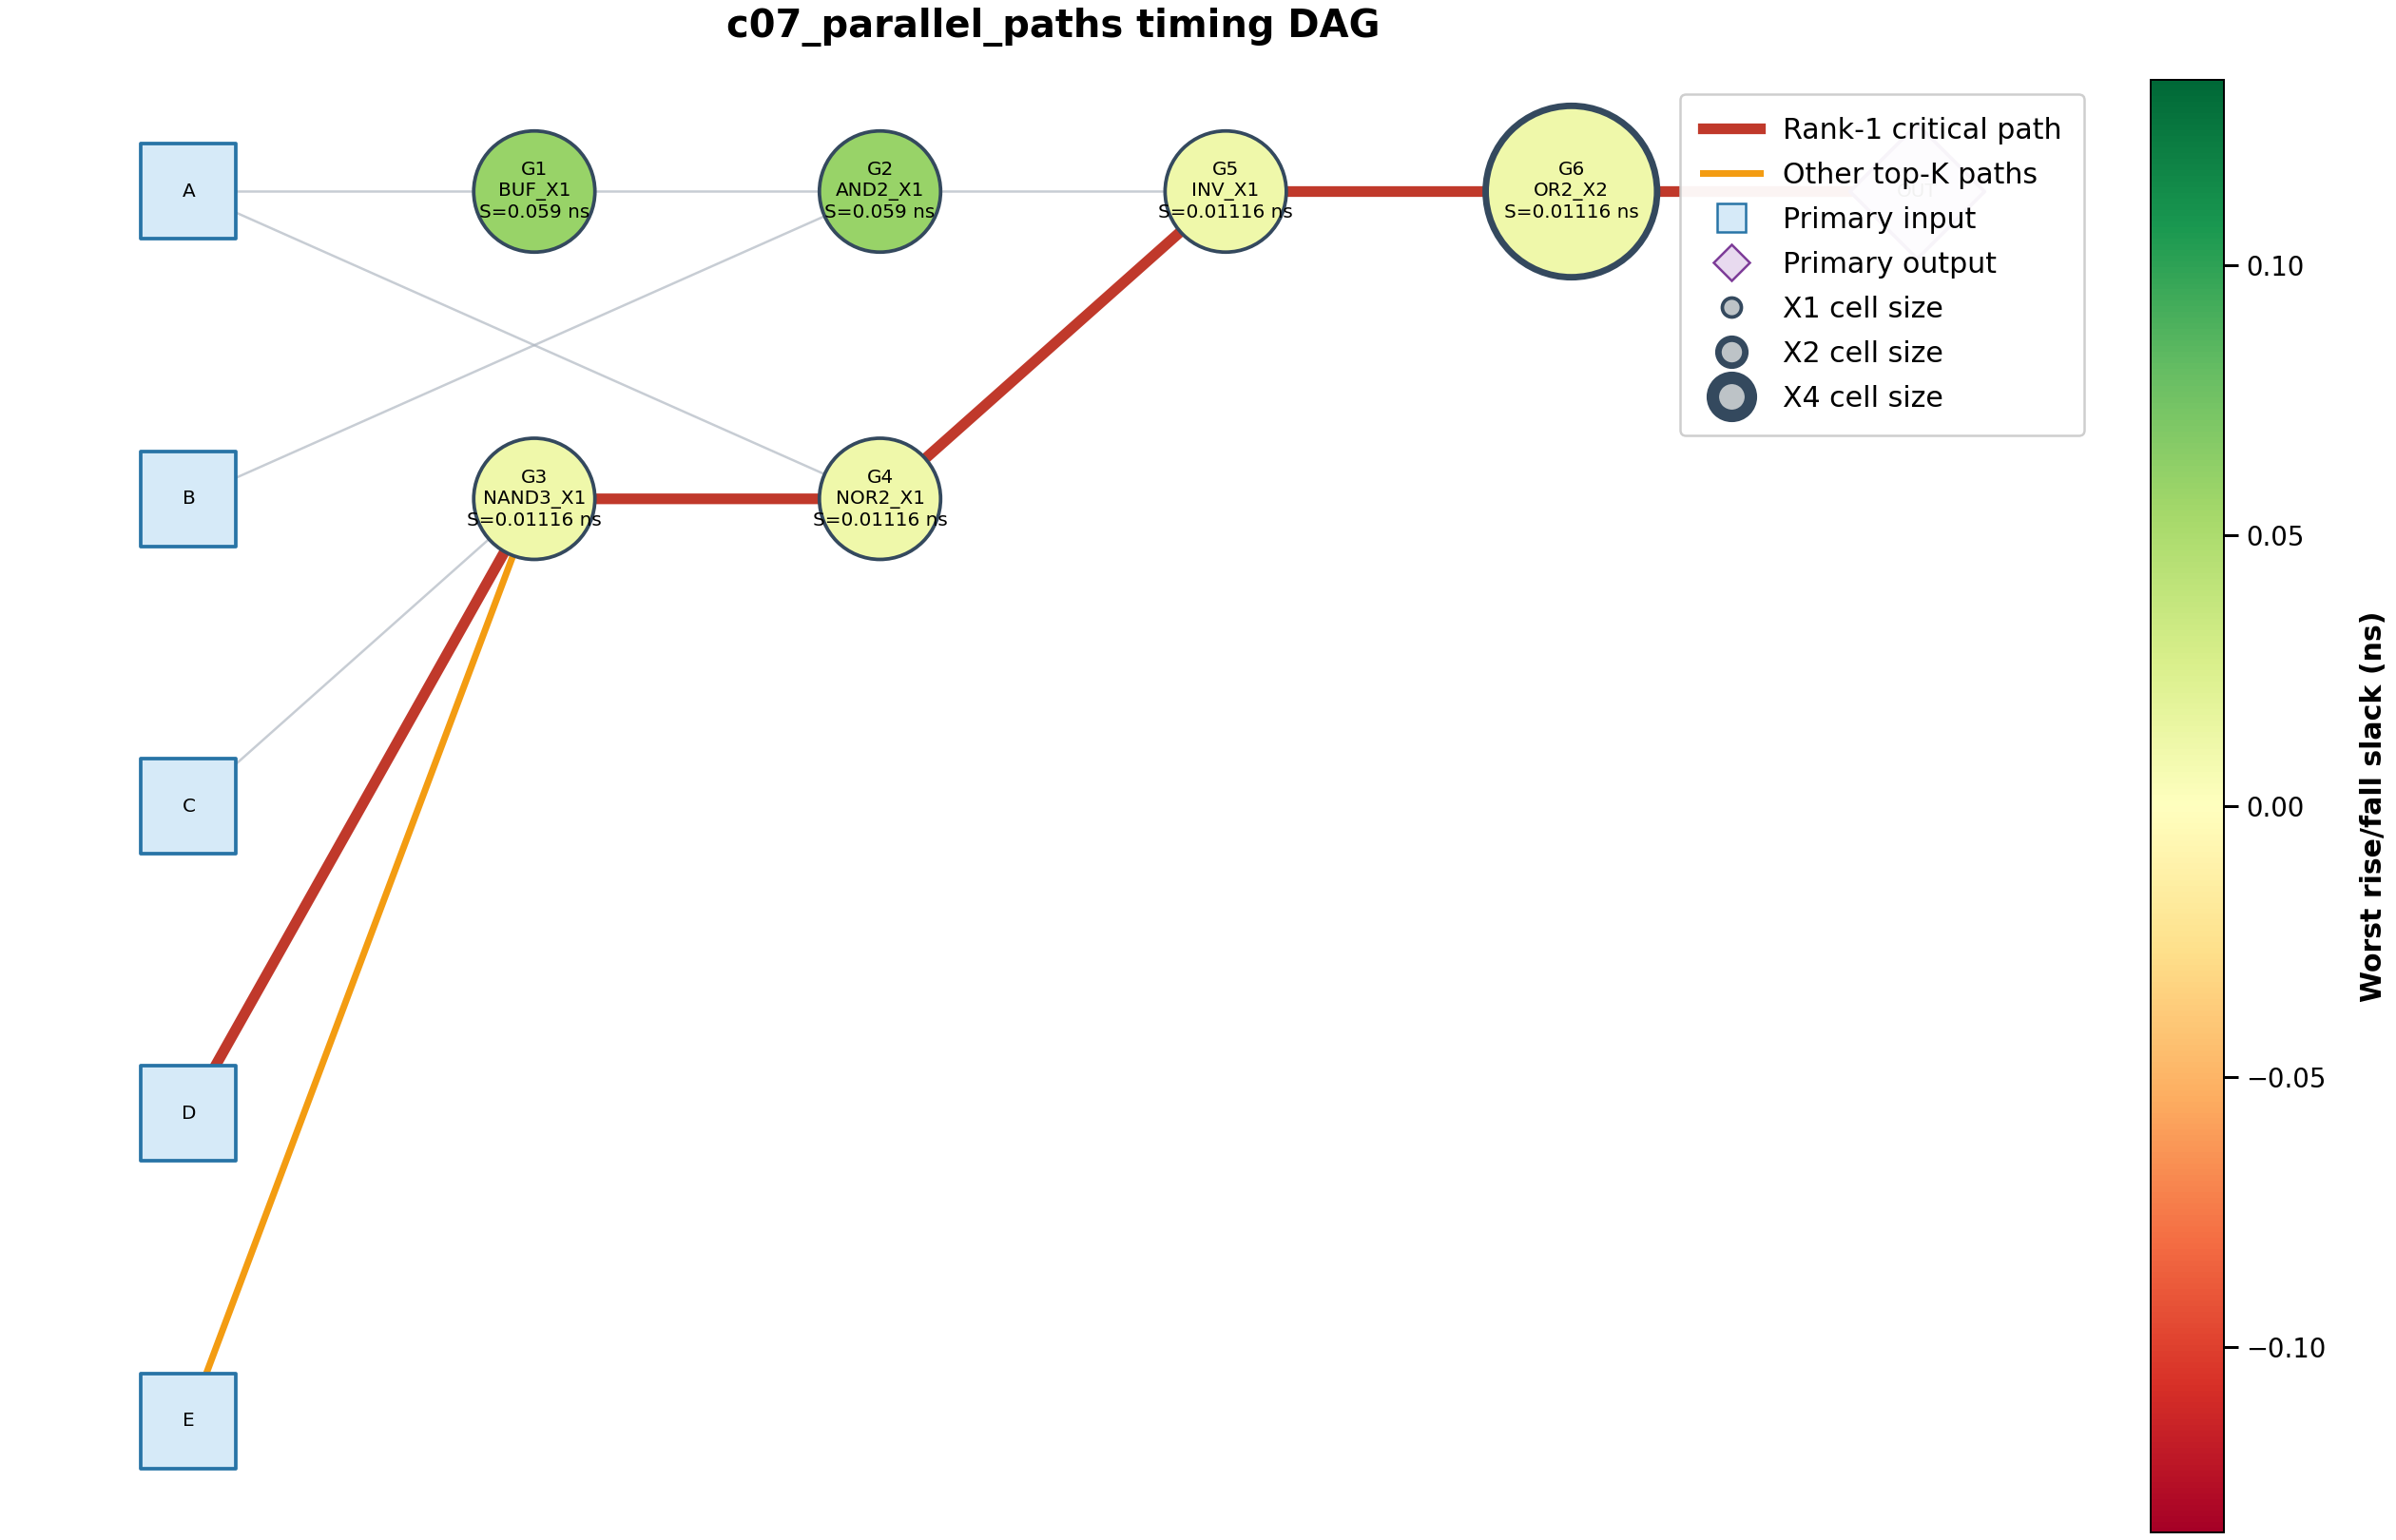
\includegraphics[width=\textwidth]{c07_parallel_paths_post.png}
        \caption{Post-optimization}
    \end{subfigure}
    \caption{\texttt{c07\_parallel\_paths}: circuit diagrams, nodes colored by slack,
    critical path highlighted.}
    \label{fig:app-c07-parallel-paths-graphs}
\end{figure}

\begin{figure}[H]
    \centering
    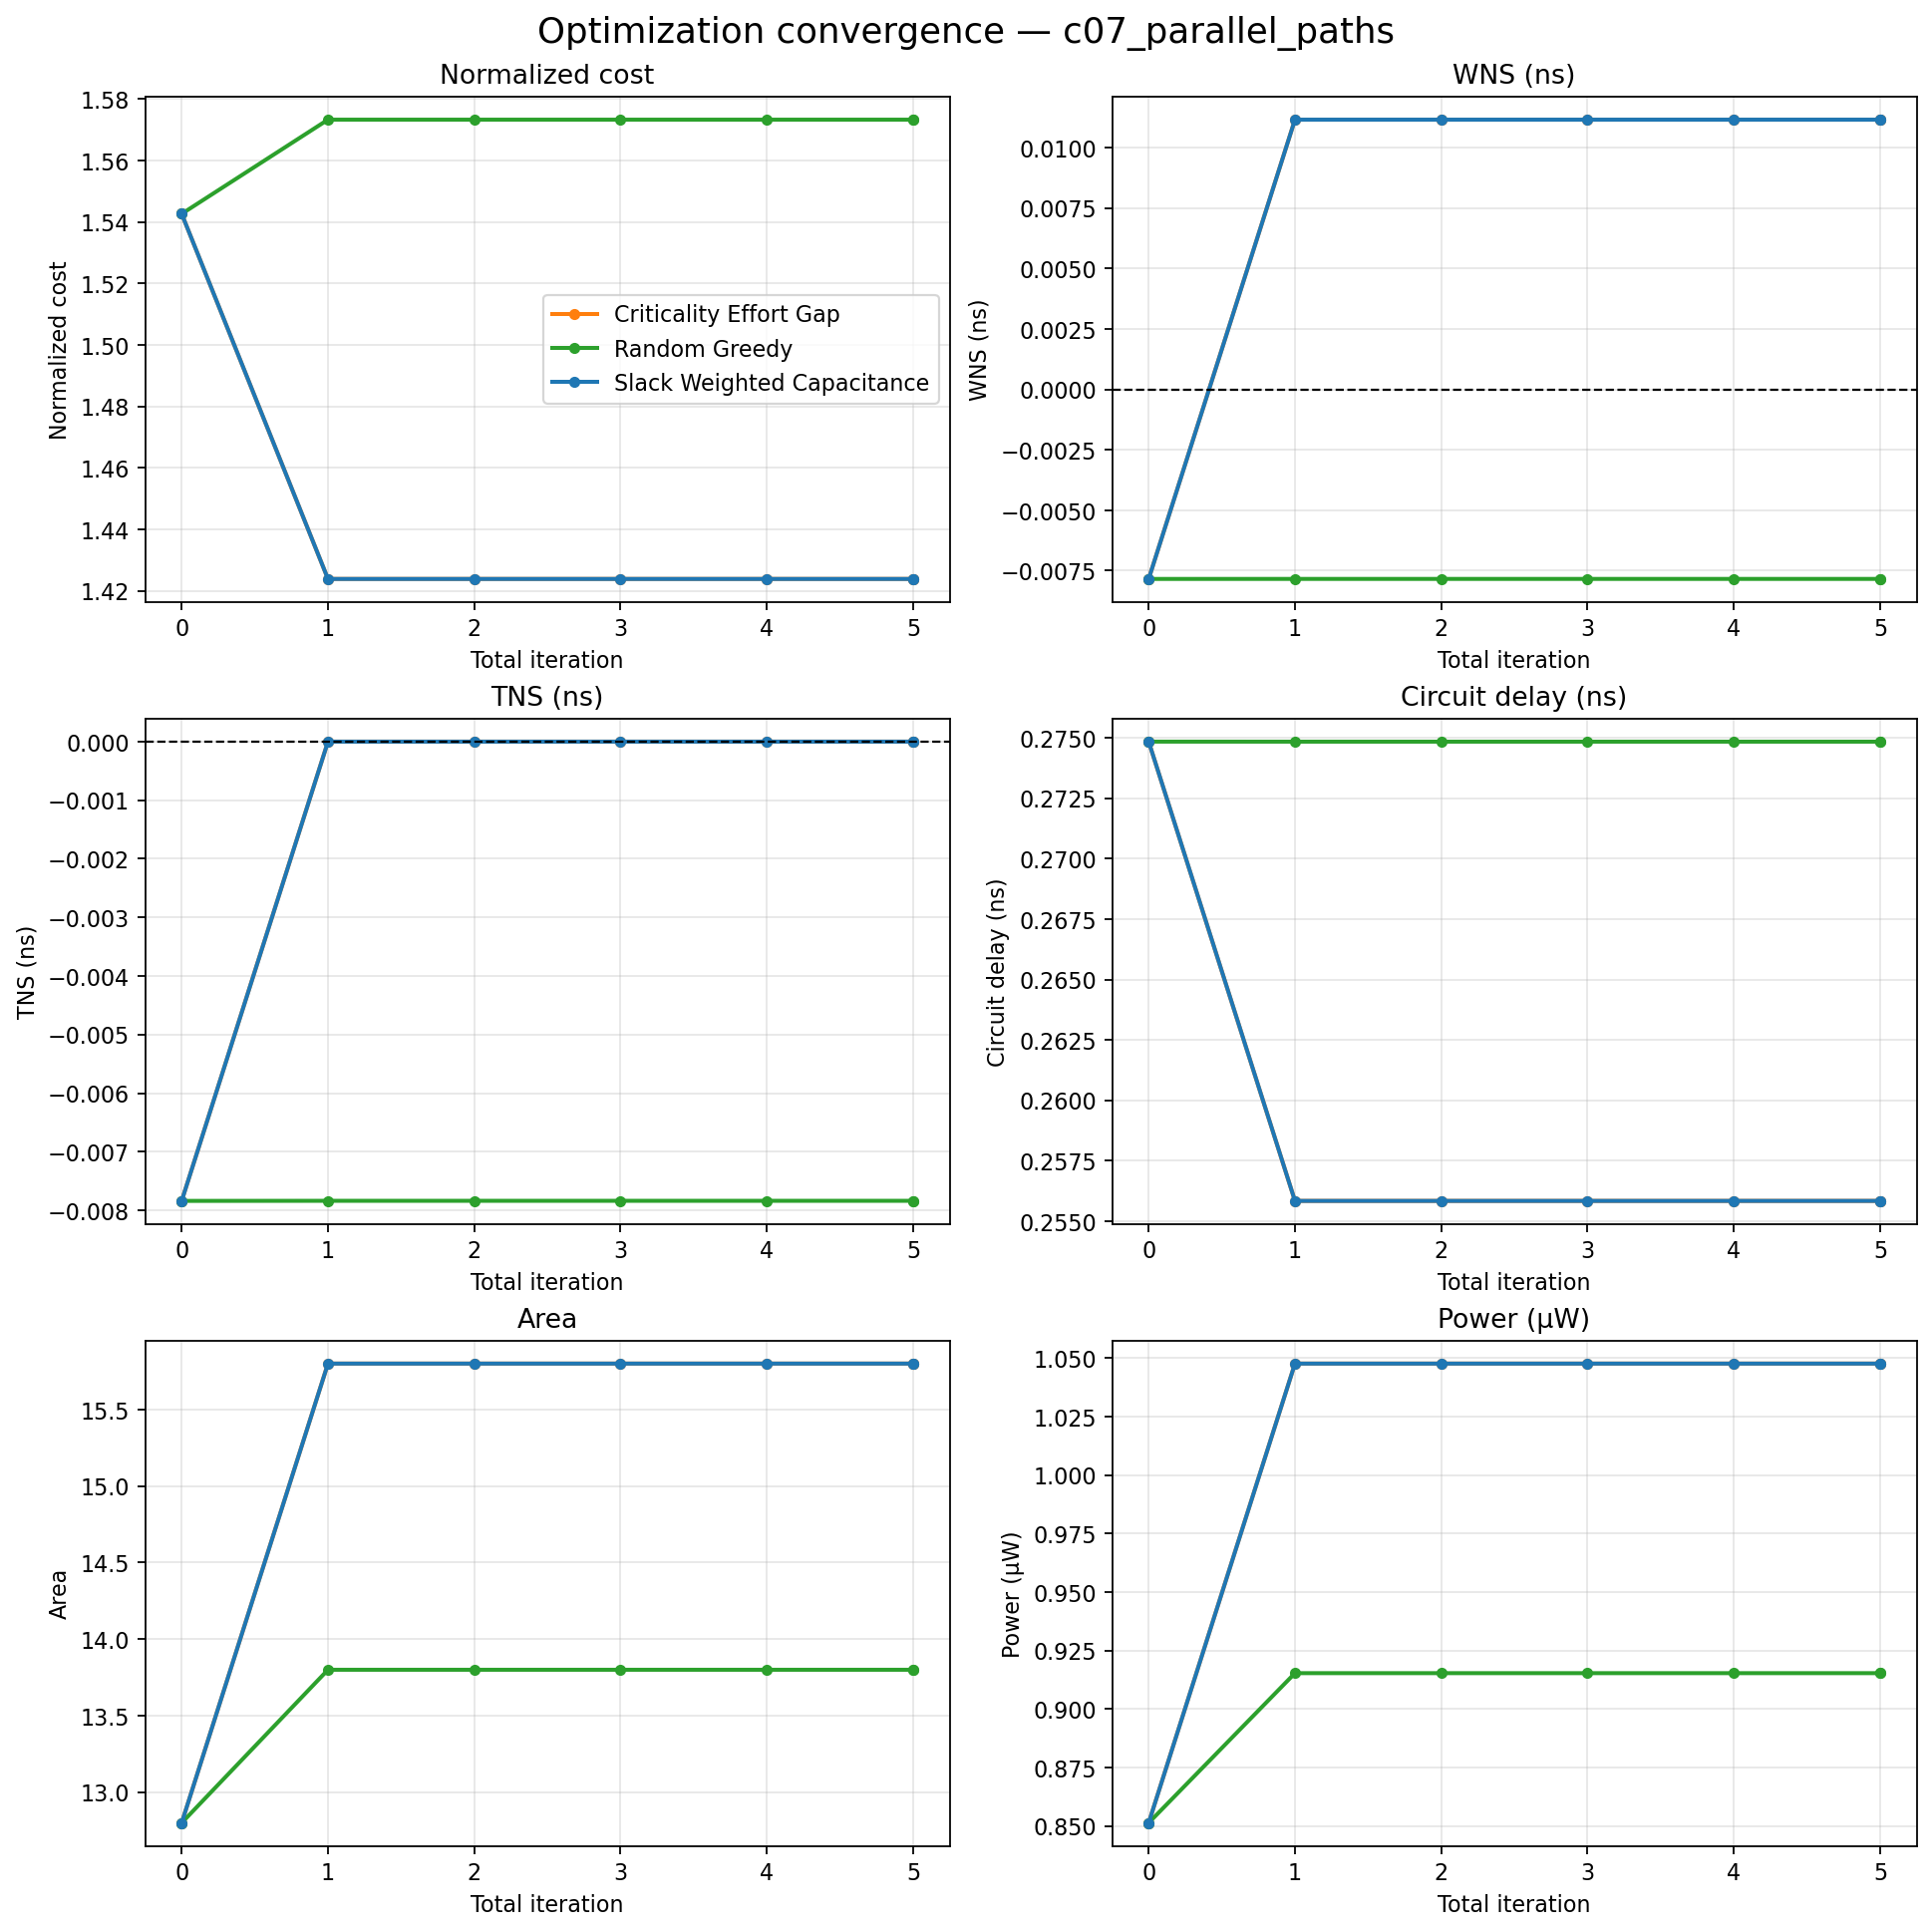
\includegraphics[width=\textwidth]{c07_parallel_paths_conv.png}
    \caption{\texttt{c07\_parallel\_paths}: optimization convergence trace.}
    \label{fig:app-c07-parallel-paths-conv}
\end{figure}

\begin{figure}[H]
    \centering
    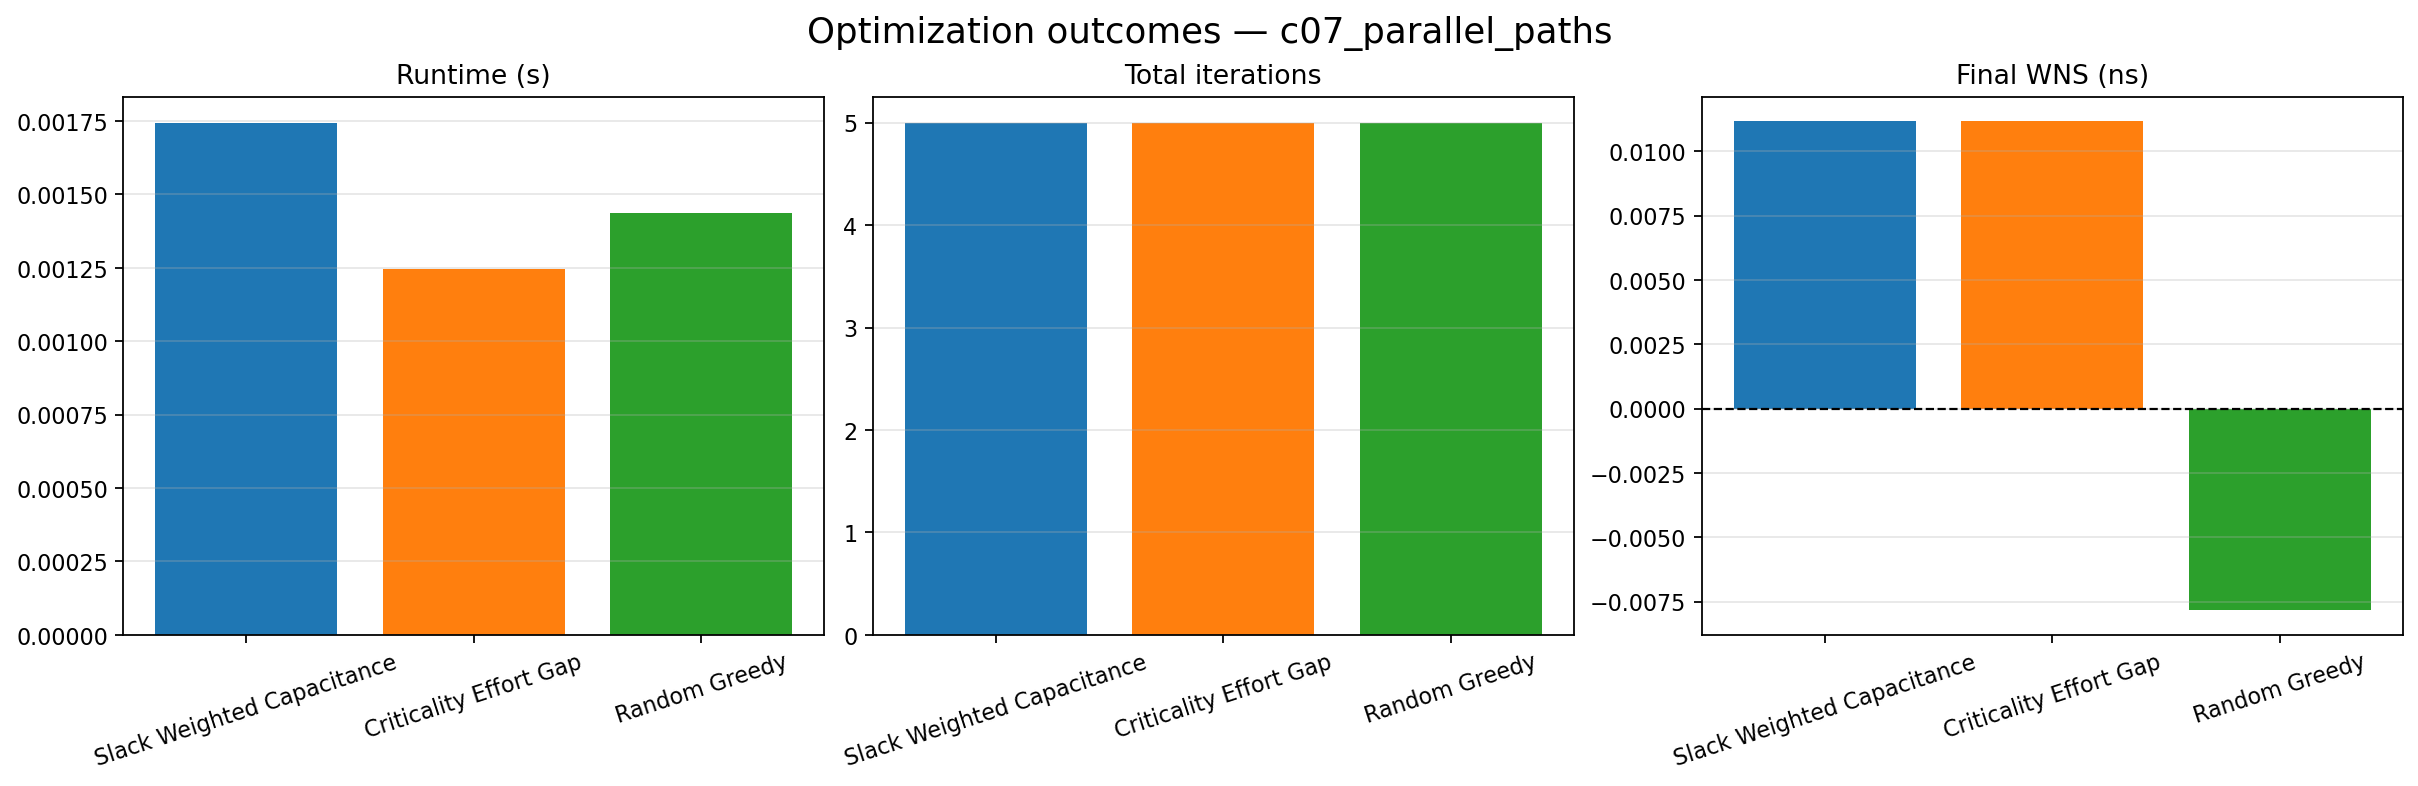
\includegraphics[width=\textwidth]{c07_parallel_paths_outc.png}
    \caption{\texttt{c07\_parallel\_paths}: optimization outcomes summary.}
    \label{fig:app-c07-parallel-paths-outc}
\end{figure}

\clearpage

\section{\texttt{c08\_non\_unate\_logic} (4 gates)}
\label{app:fig-c08-non-unate-logic}

\begin{figure}[H]
    \centering
    \begin{subfigure}[t]{0.48\textwidth}
        \centering
        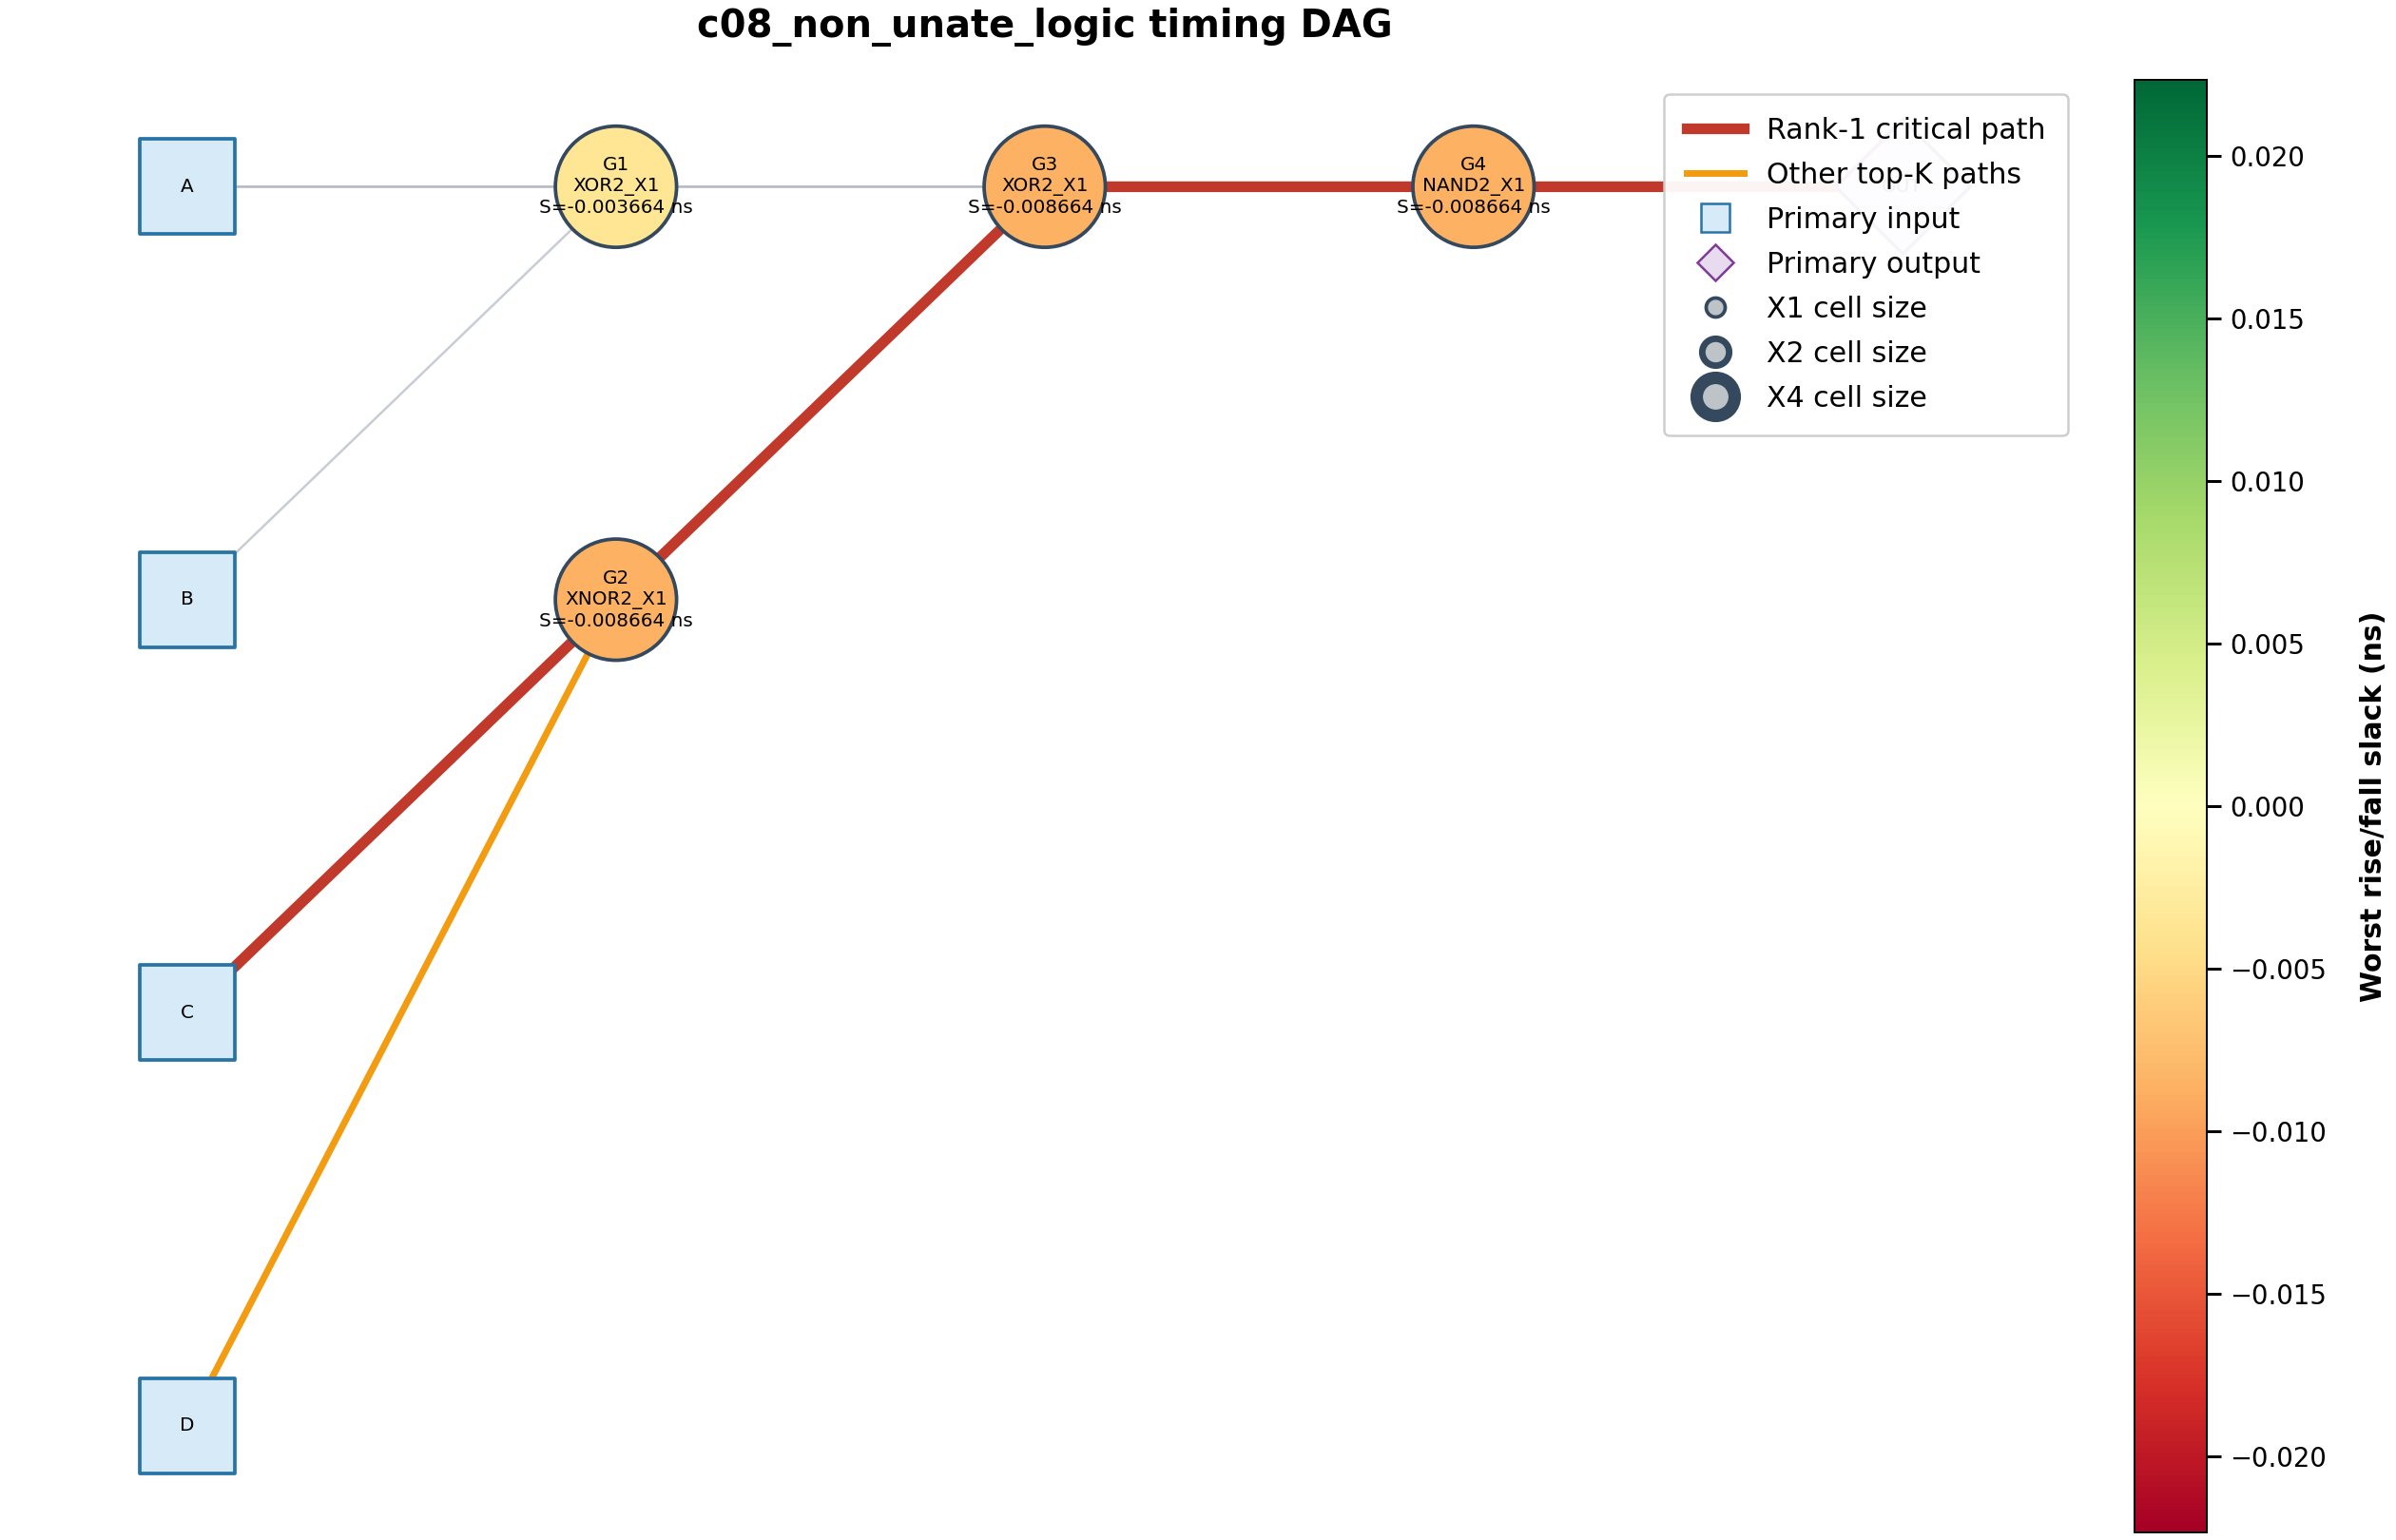
\includegraphics[width=\textwidth]{c08_non_unate_logic_pre.png}
        \caption{Pre-optimization}
    \end{subfigure}
    \hfill
    \begin{subfigure}[t]{0.48\textwidth}
        \centering
        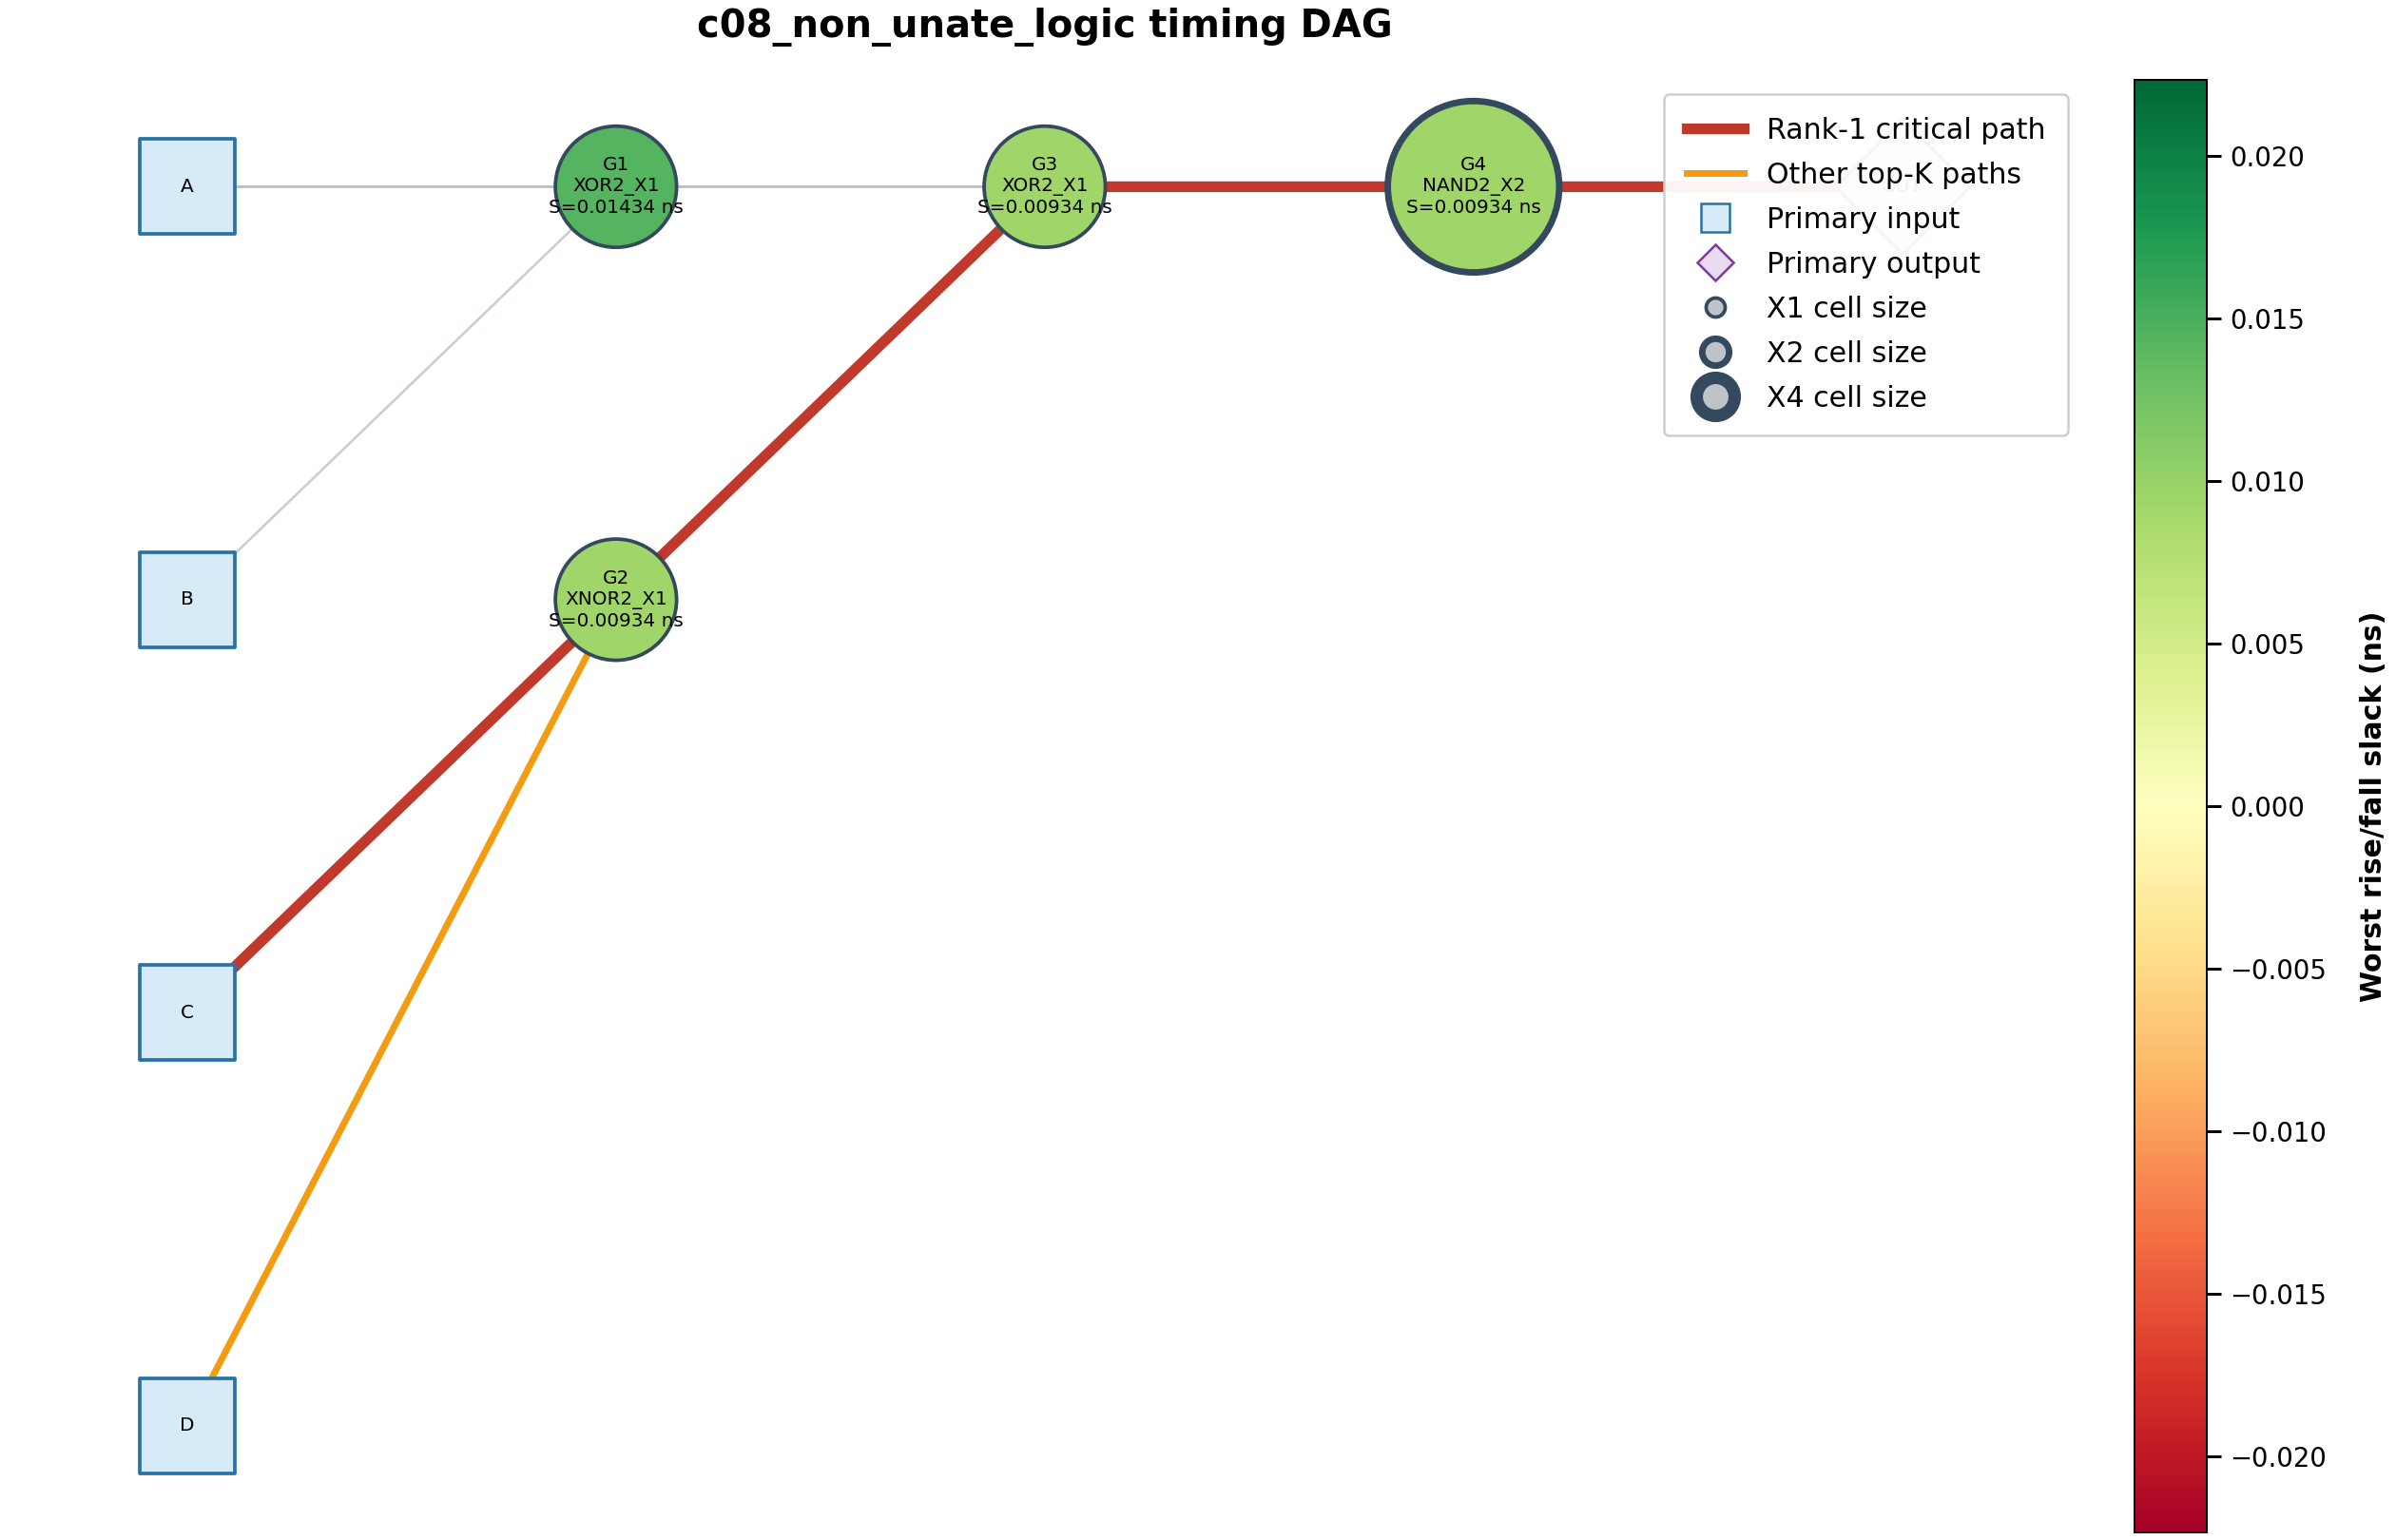
\includegraphics[width=\textwidth]{c08_non_unate_logic_post.png}
        \caption{Post-optimization}
    \end{subfigure}
    \caption{\texttt{c08\_non\_unate\_logic}: circuit diagrams, nodes colored by slack,
    critical path highlighted.}
    \label{fig:app-c08-non-unate-logic-graphs}
\end{figure}

\begin{figure}[H]
    \centering
    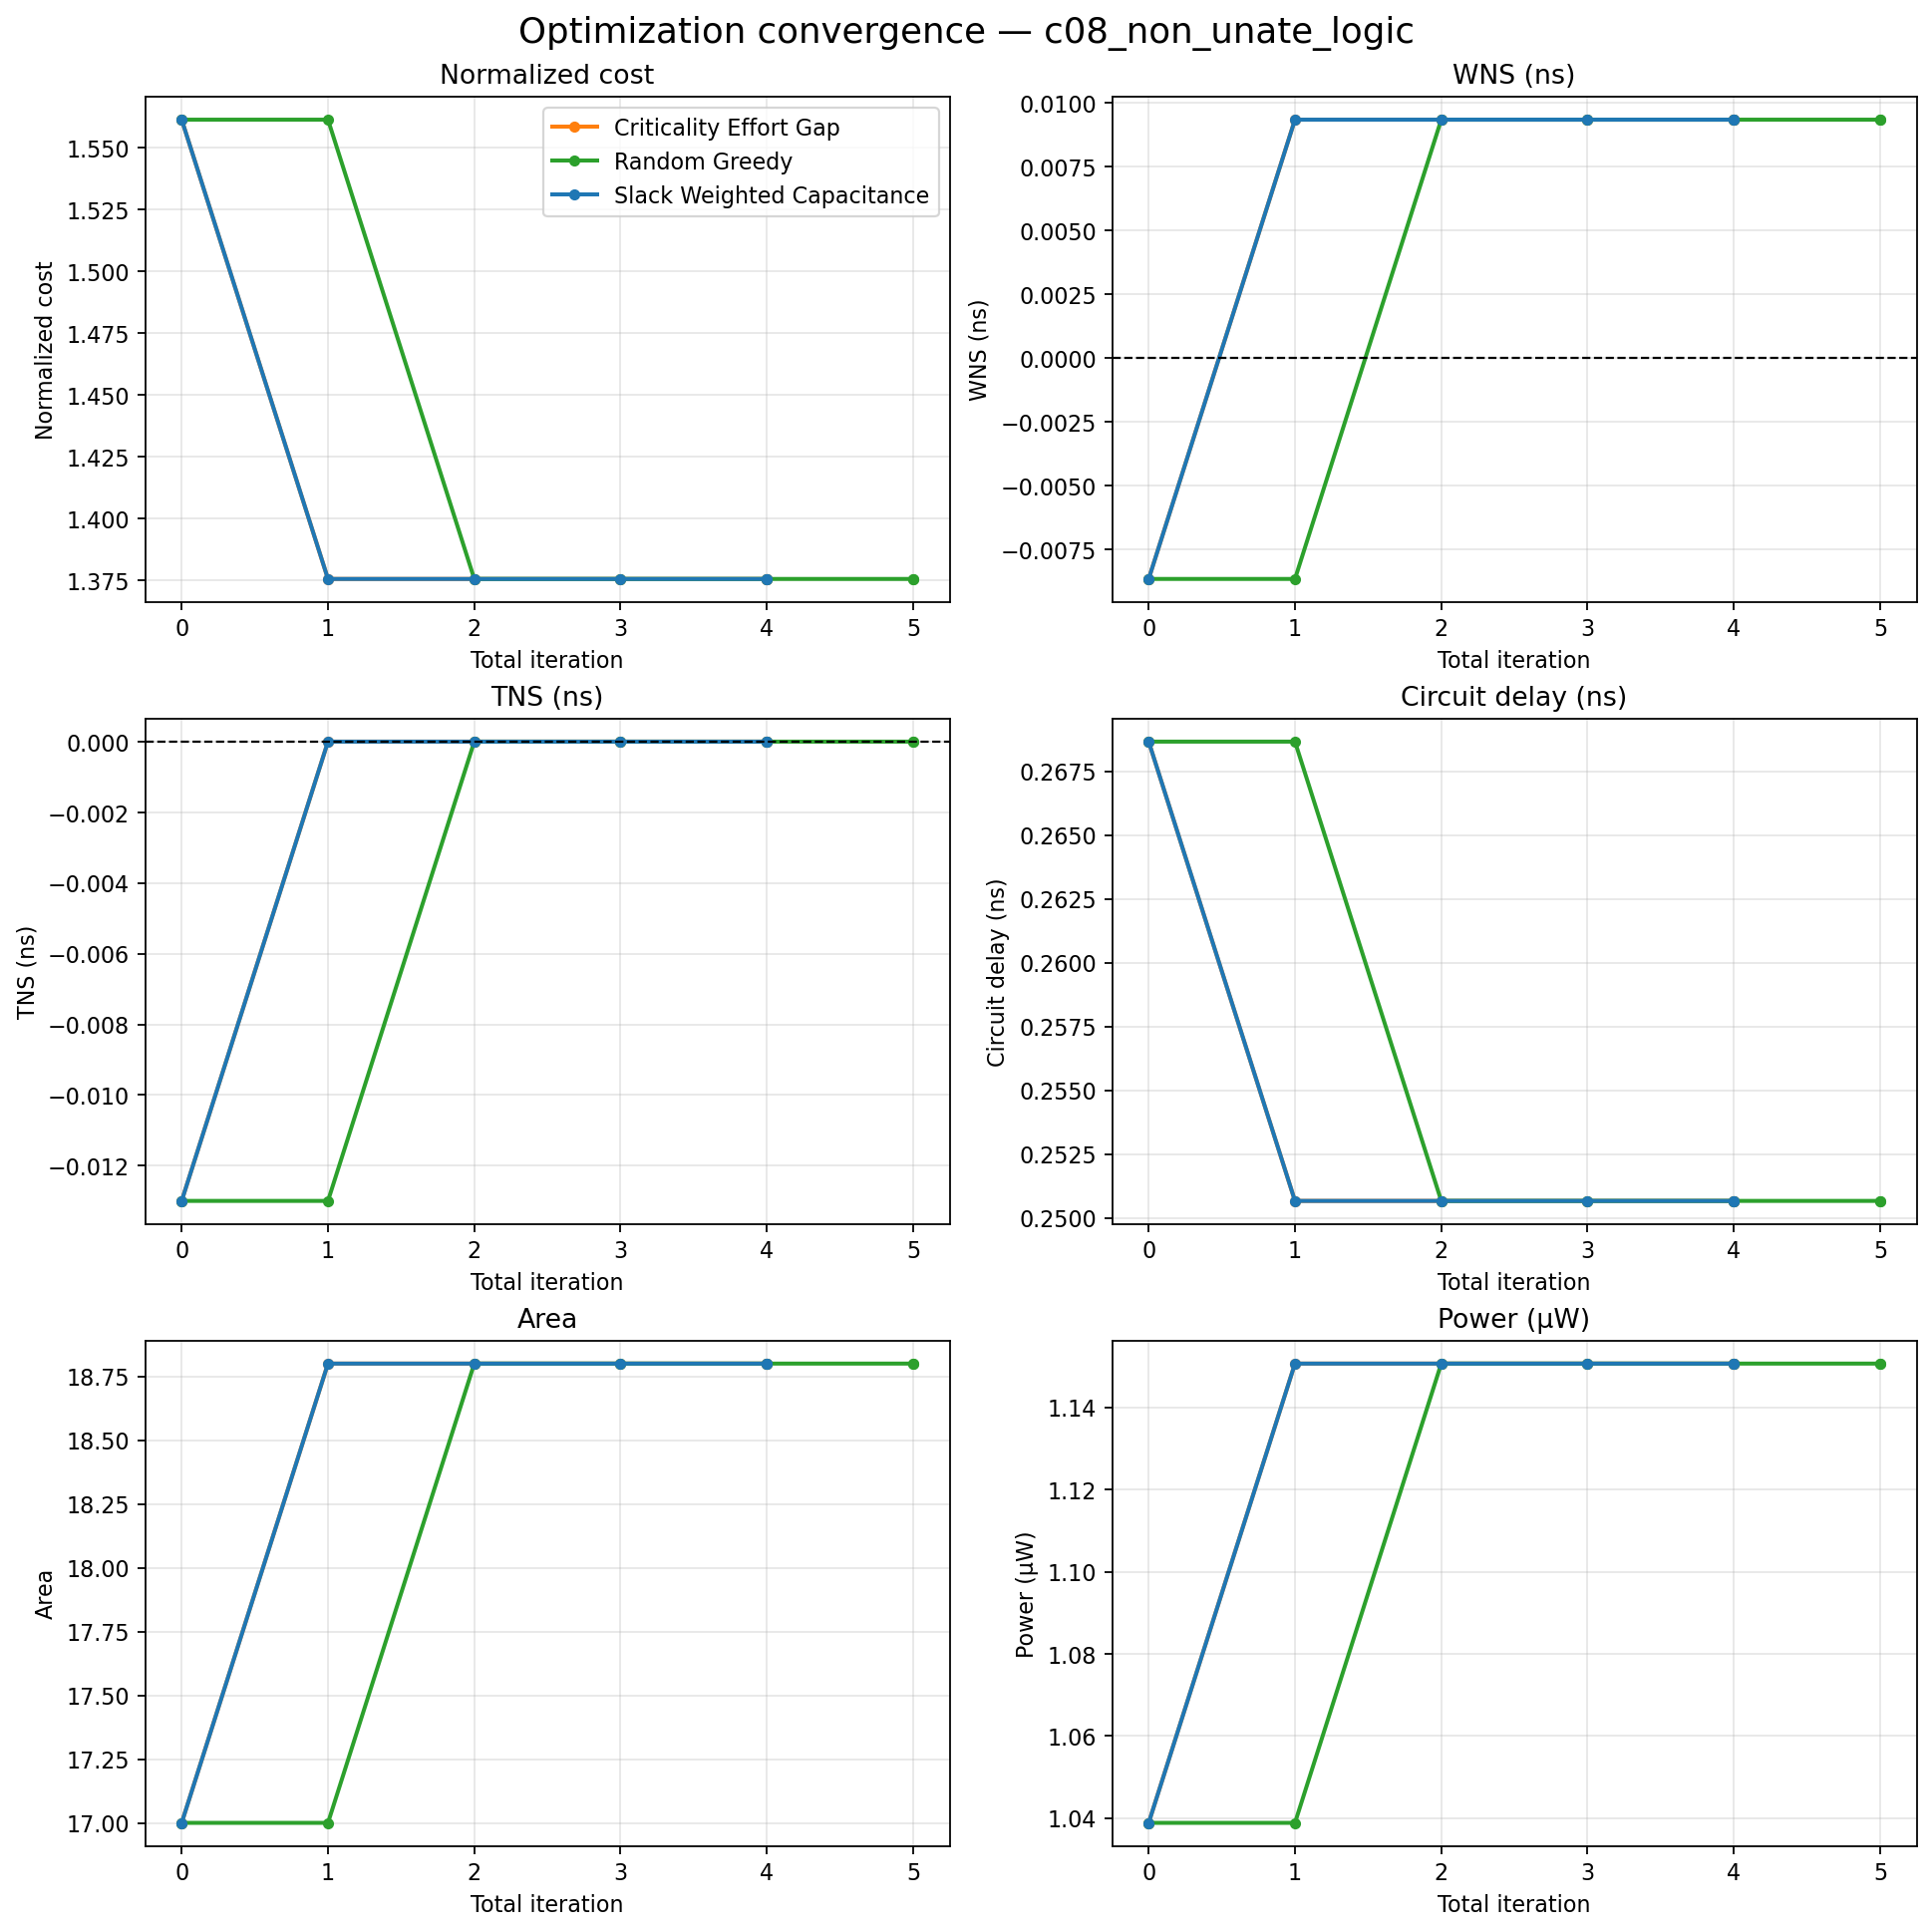
\includegraphics[width=\textwidth]{c08_non_unate_logic_conv.png}
    \caption{\texttt{c08\_non\_unate\_logic}: optimization convergence trace.}
    \label{fig:app-c08-non-unate-logic-conv}
\end{figure}

\begin{figure}[H]
    \centering
    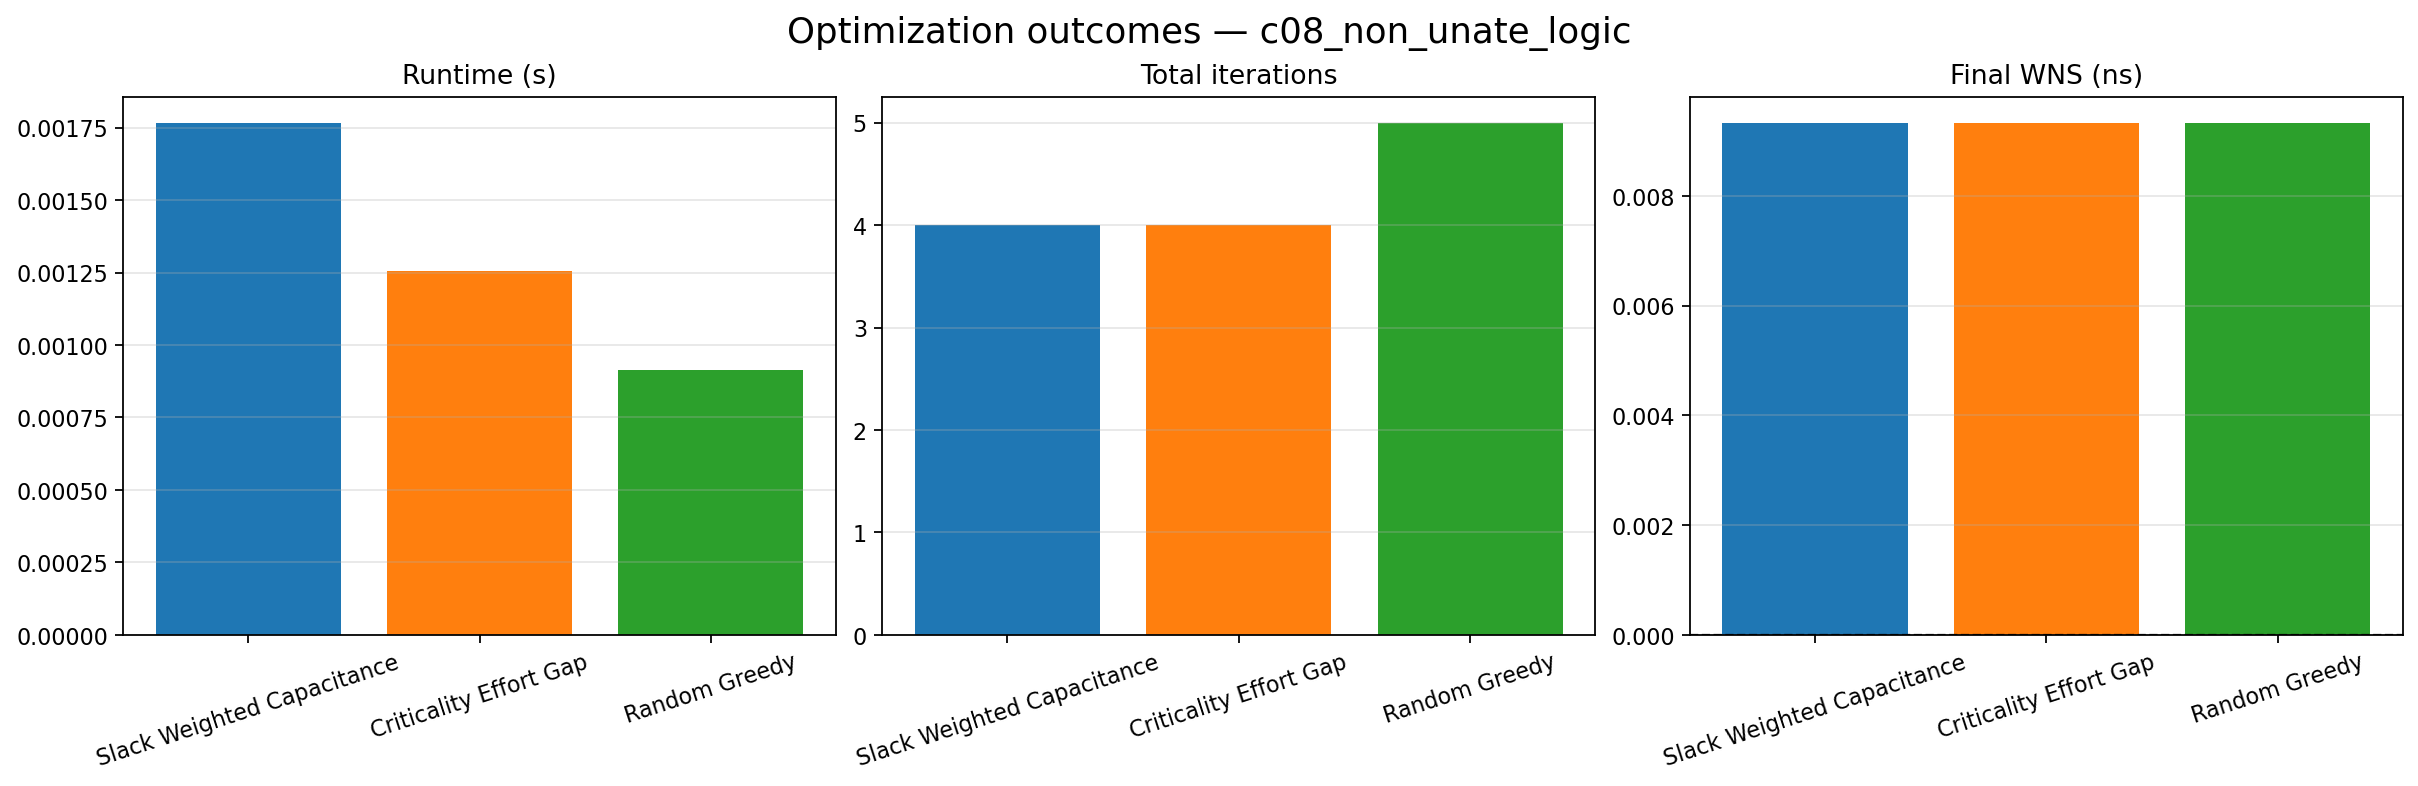
\includegraphics[width=\textwidth]{c08_non_unate_logic_outc.png}
    \caption{\texttt{c08\_non\_unate\_logic}: optimization outcomes summary.}
    \label{fig:app-c08-non-unate-logic-outc}
\end{figure}

\clearpage

\section{\texttt{c09\_high\_fanout} (6 gates)}
\label{app:fig-c09-high-fanout}

\begin{figure}[H]
    \centering
    \begin{subfigure}[t]{0.48\textwidth}
        \centering
        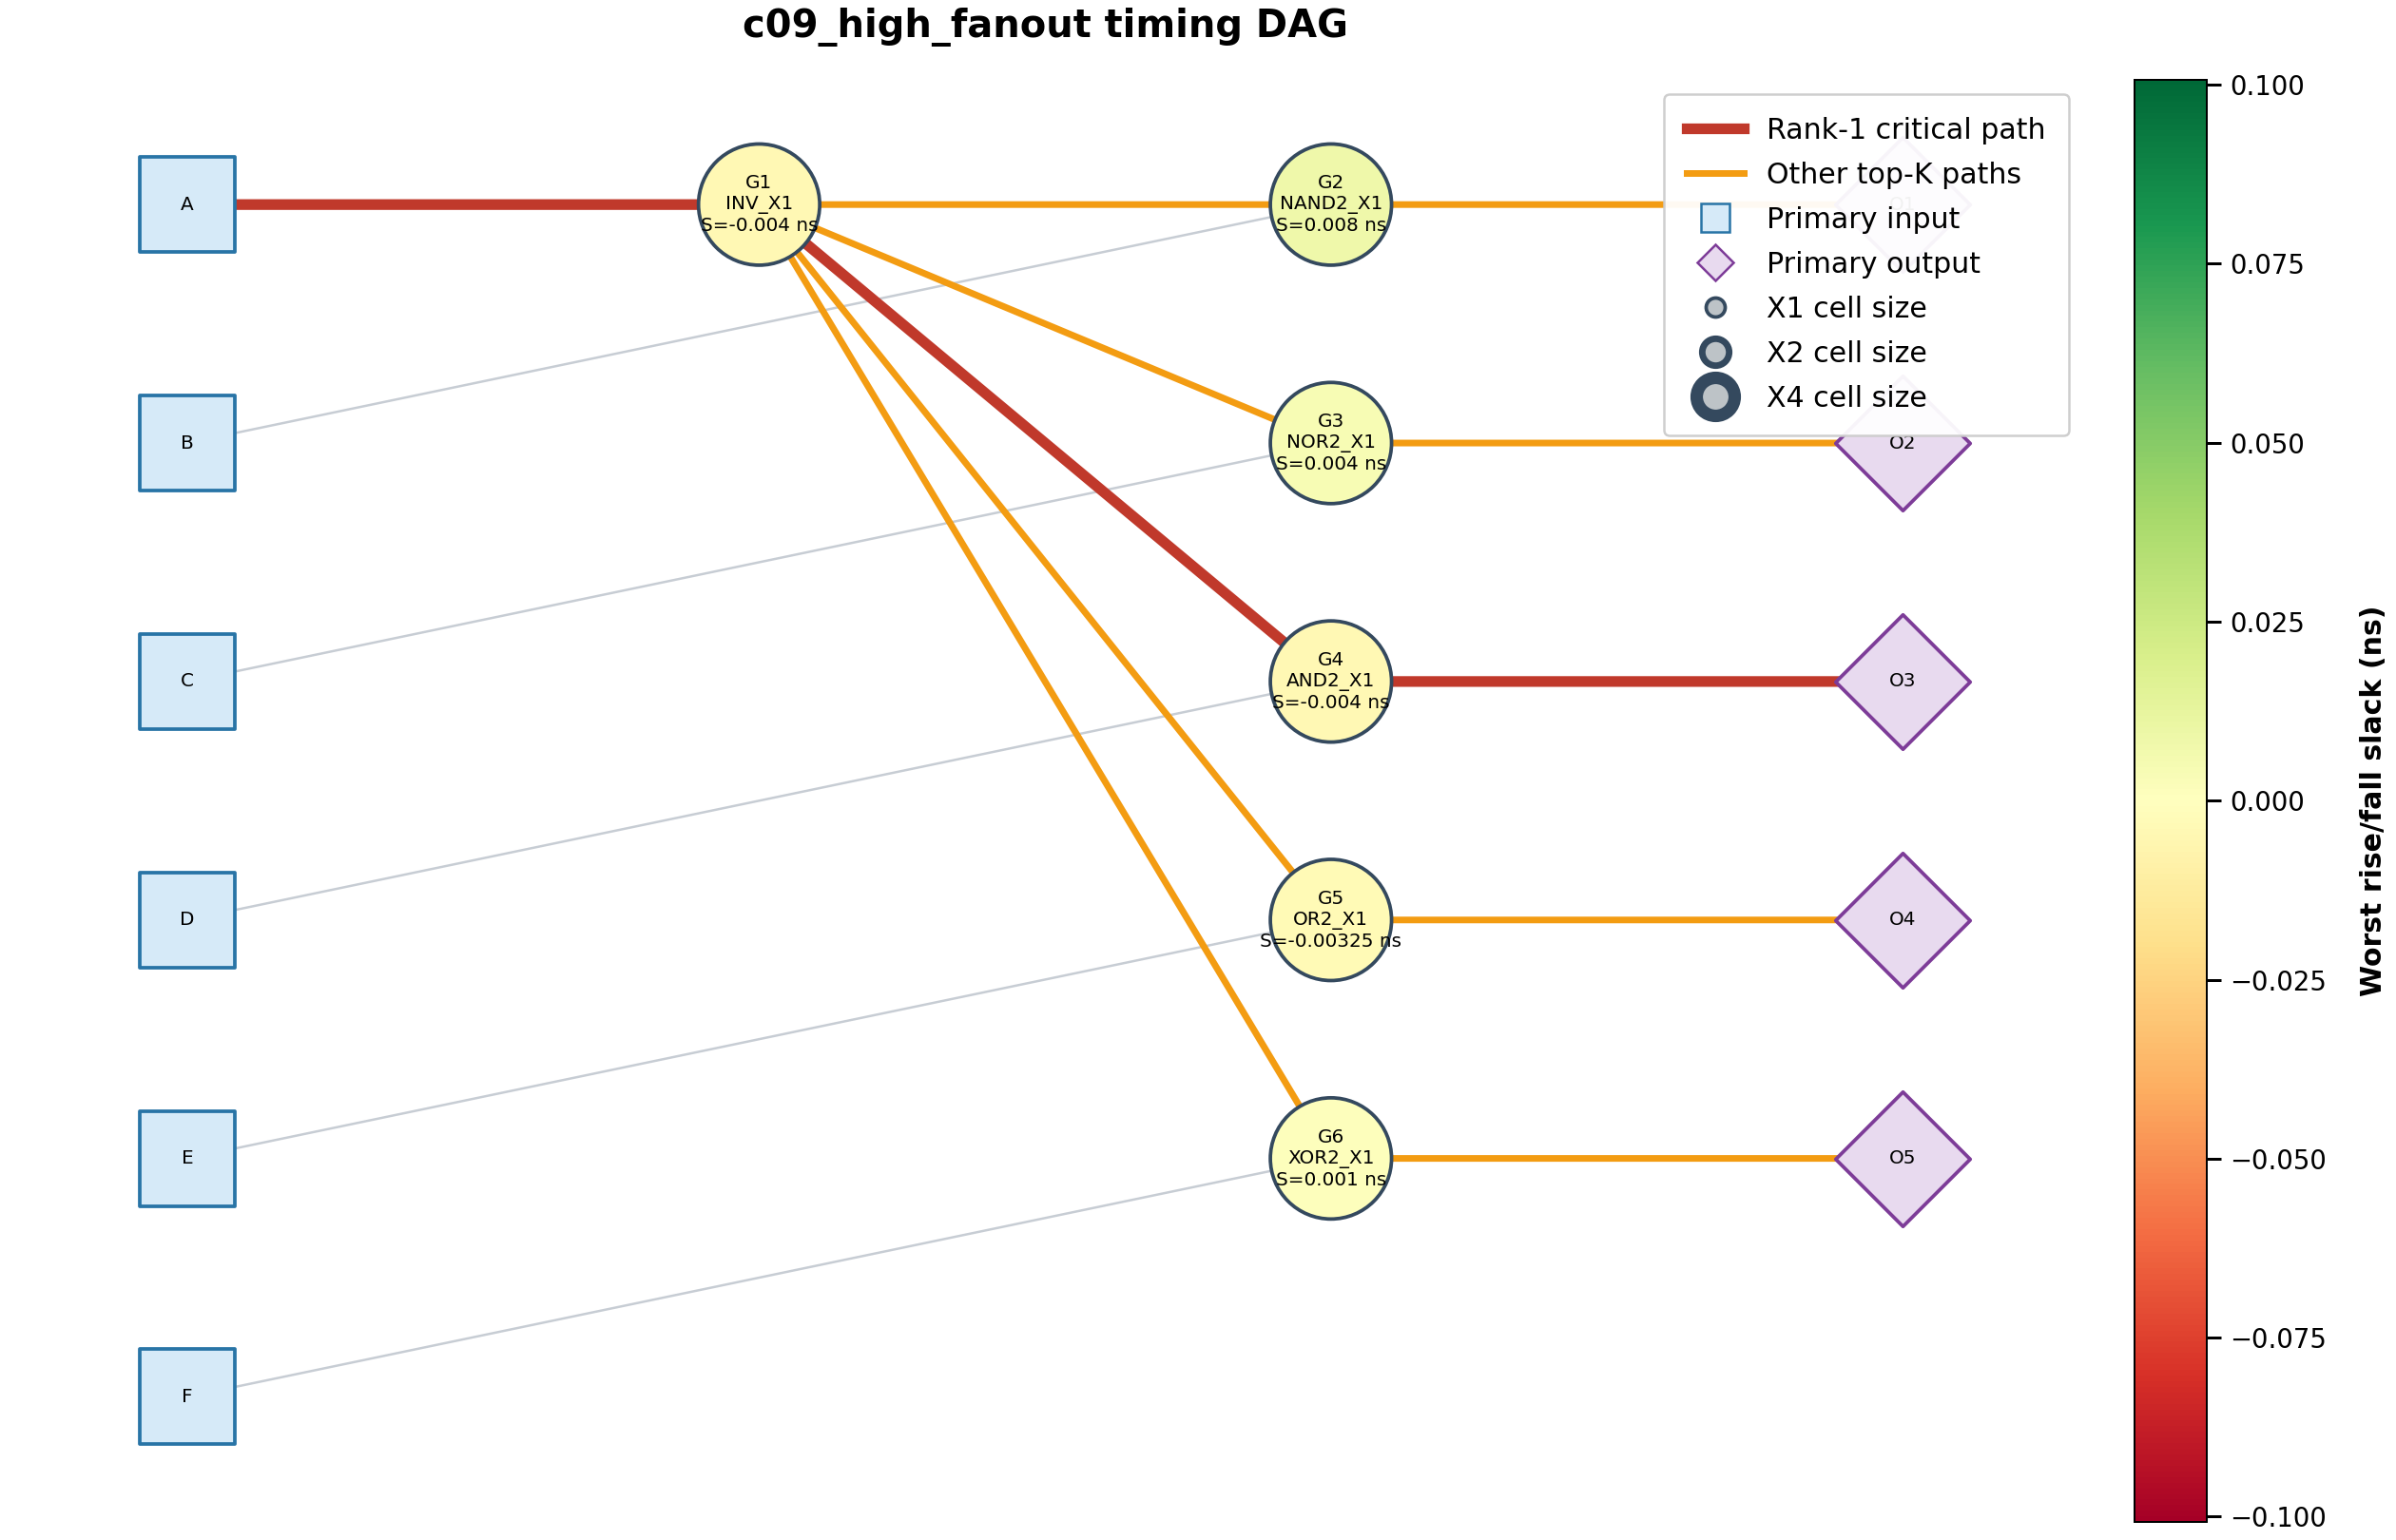
\includegraphics[width=\textwidth]{c09_high_fanout_pre.png}
        \caption{Pre-optimization}
    \end{subfigure}
    \hfill
    \begin{subfigure}[t]{0.48\textwidth}
        \centering
        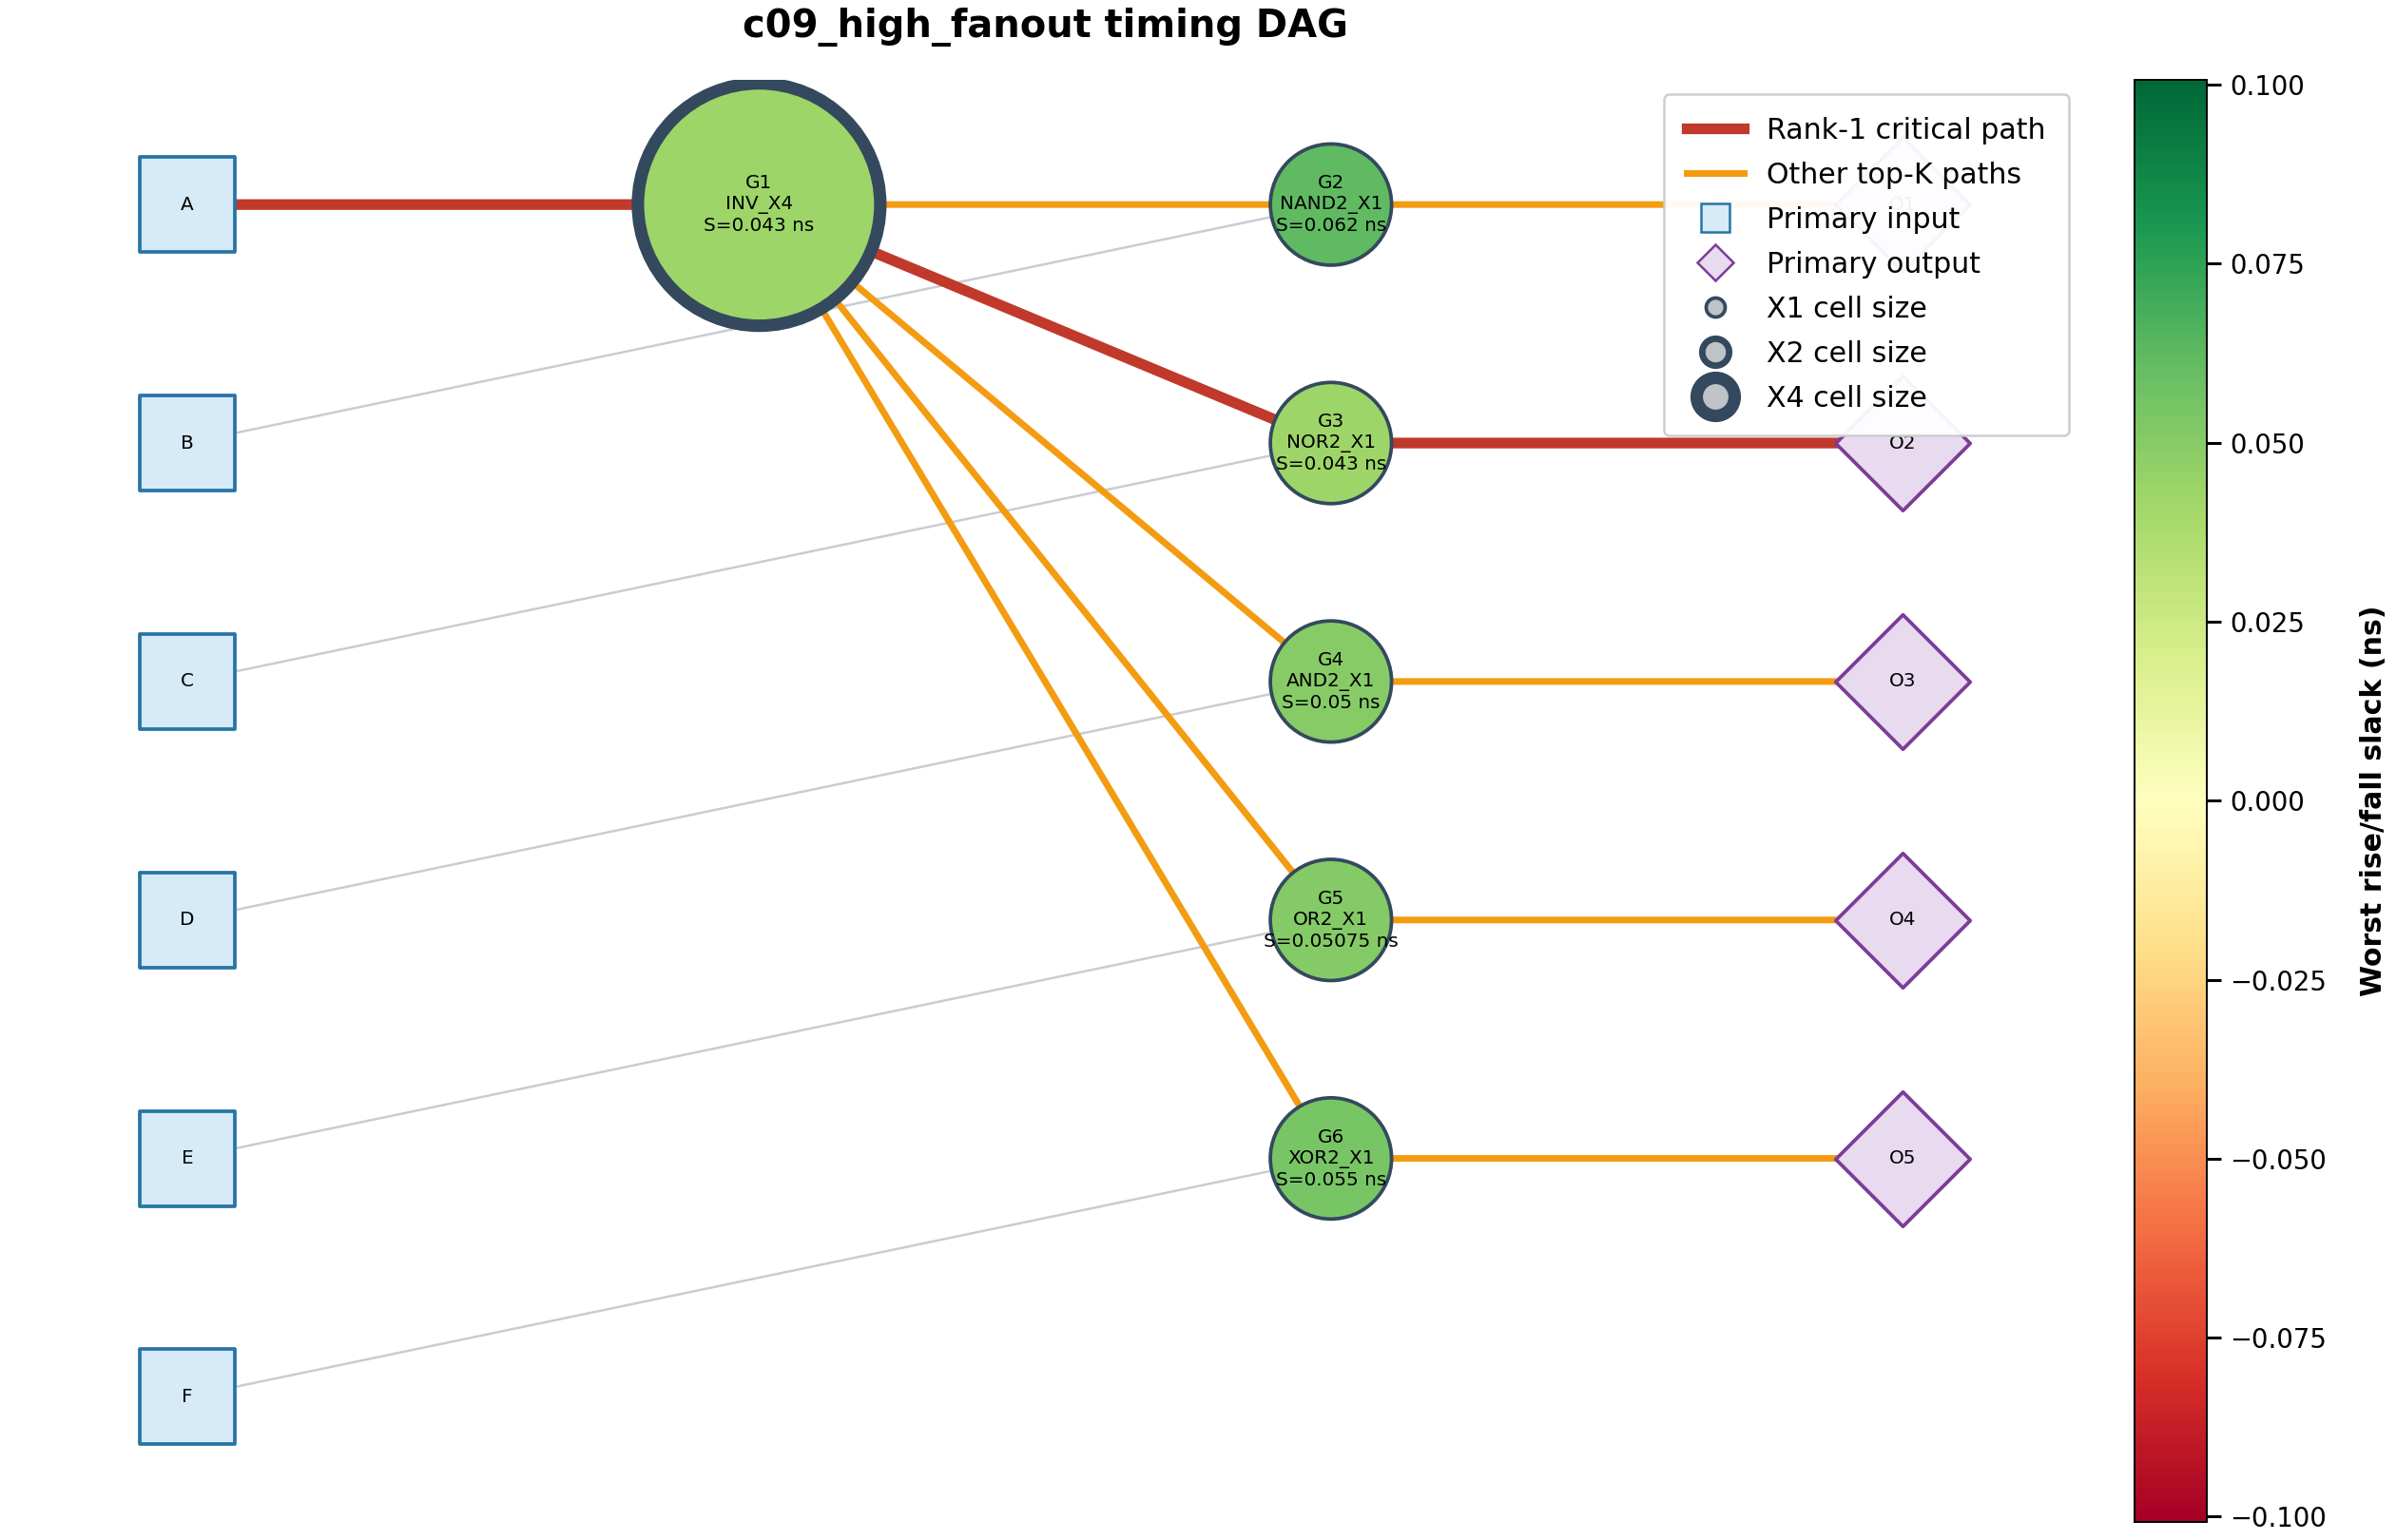
\includegraphics[width=\textwidth]{c09_high_fanout_post.png}
        \caption{Post-optimization}
    \end{subfigure}
    \caption{\texttt{c09\_high\_fanout}: circuit diagrams, nodes colored by slack,
    critical path highlighted.}
    \label{fig:app-c09-high-fanout-graphs}
\end{figure}

\begin{figure}[H]
    \centering
    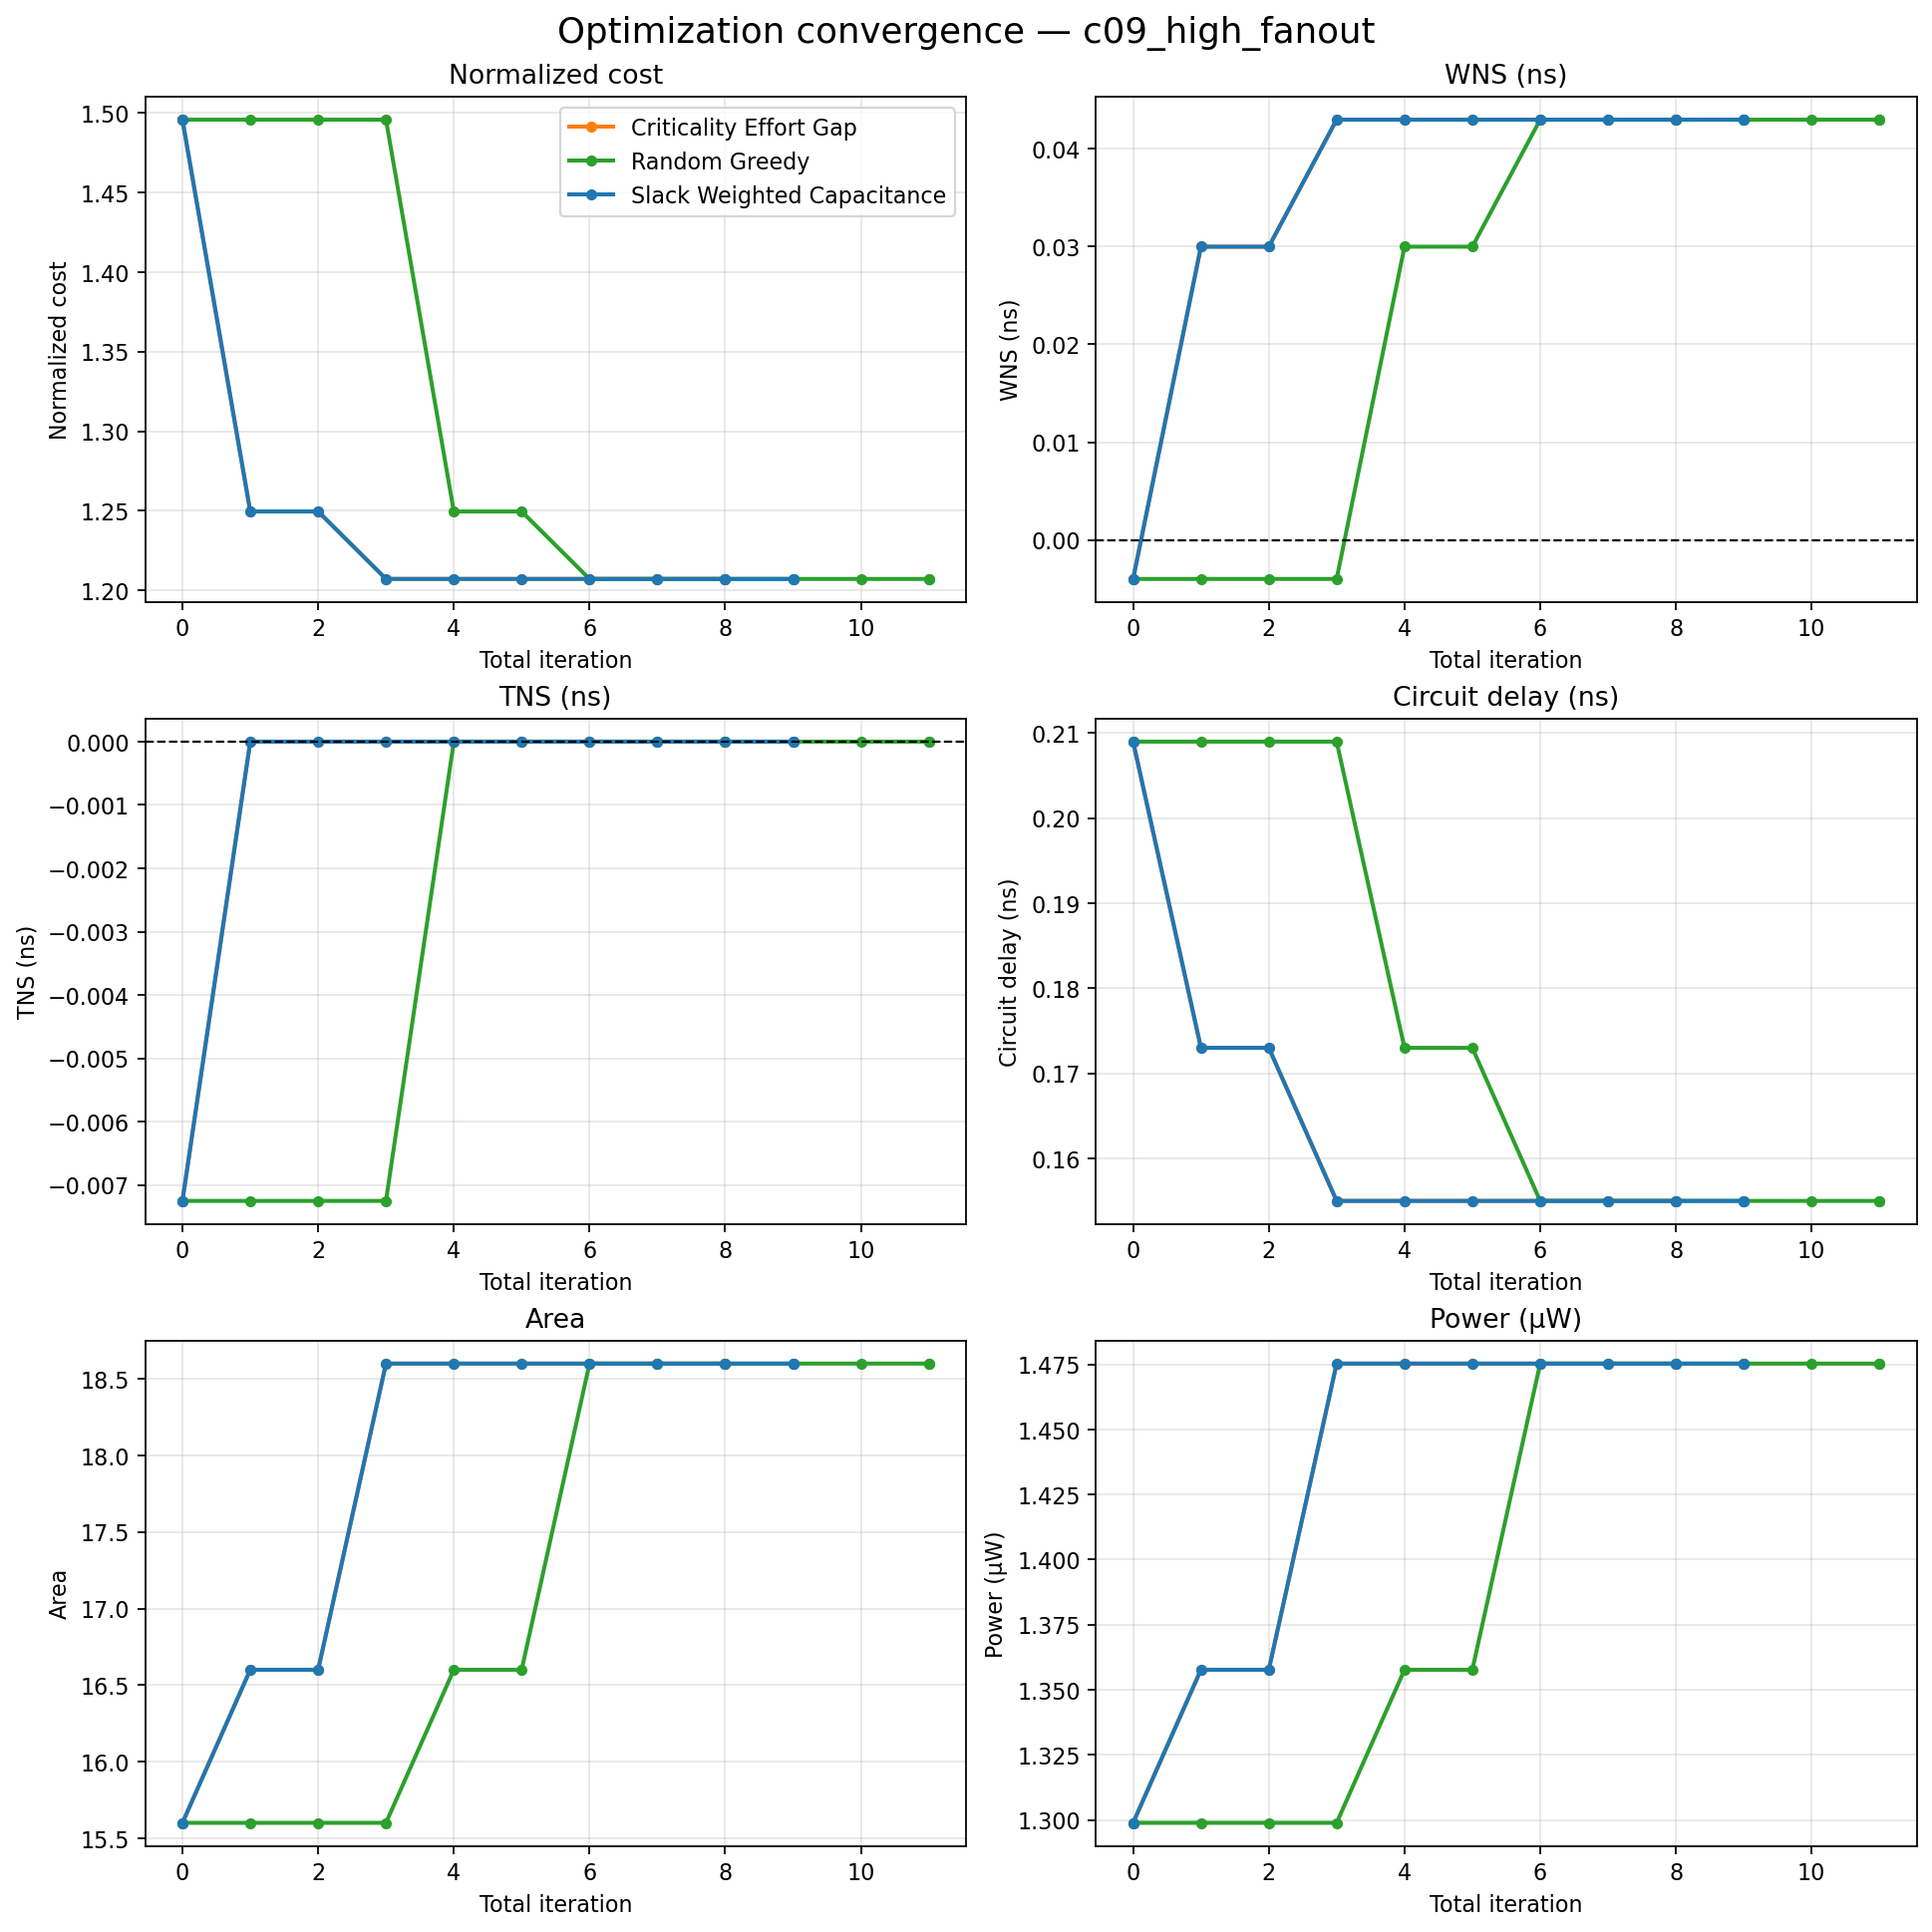
\includegraphics[width=\textwidth]{c09_high_fanout_conv.png}
    \caption{\texttt{c09\_high\_fanout}: optimization convergence trace.}
    \label{fig:app-c09-high-fanout-conv}
\end{figure}

\begin{figure}[H]
    \centering
    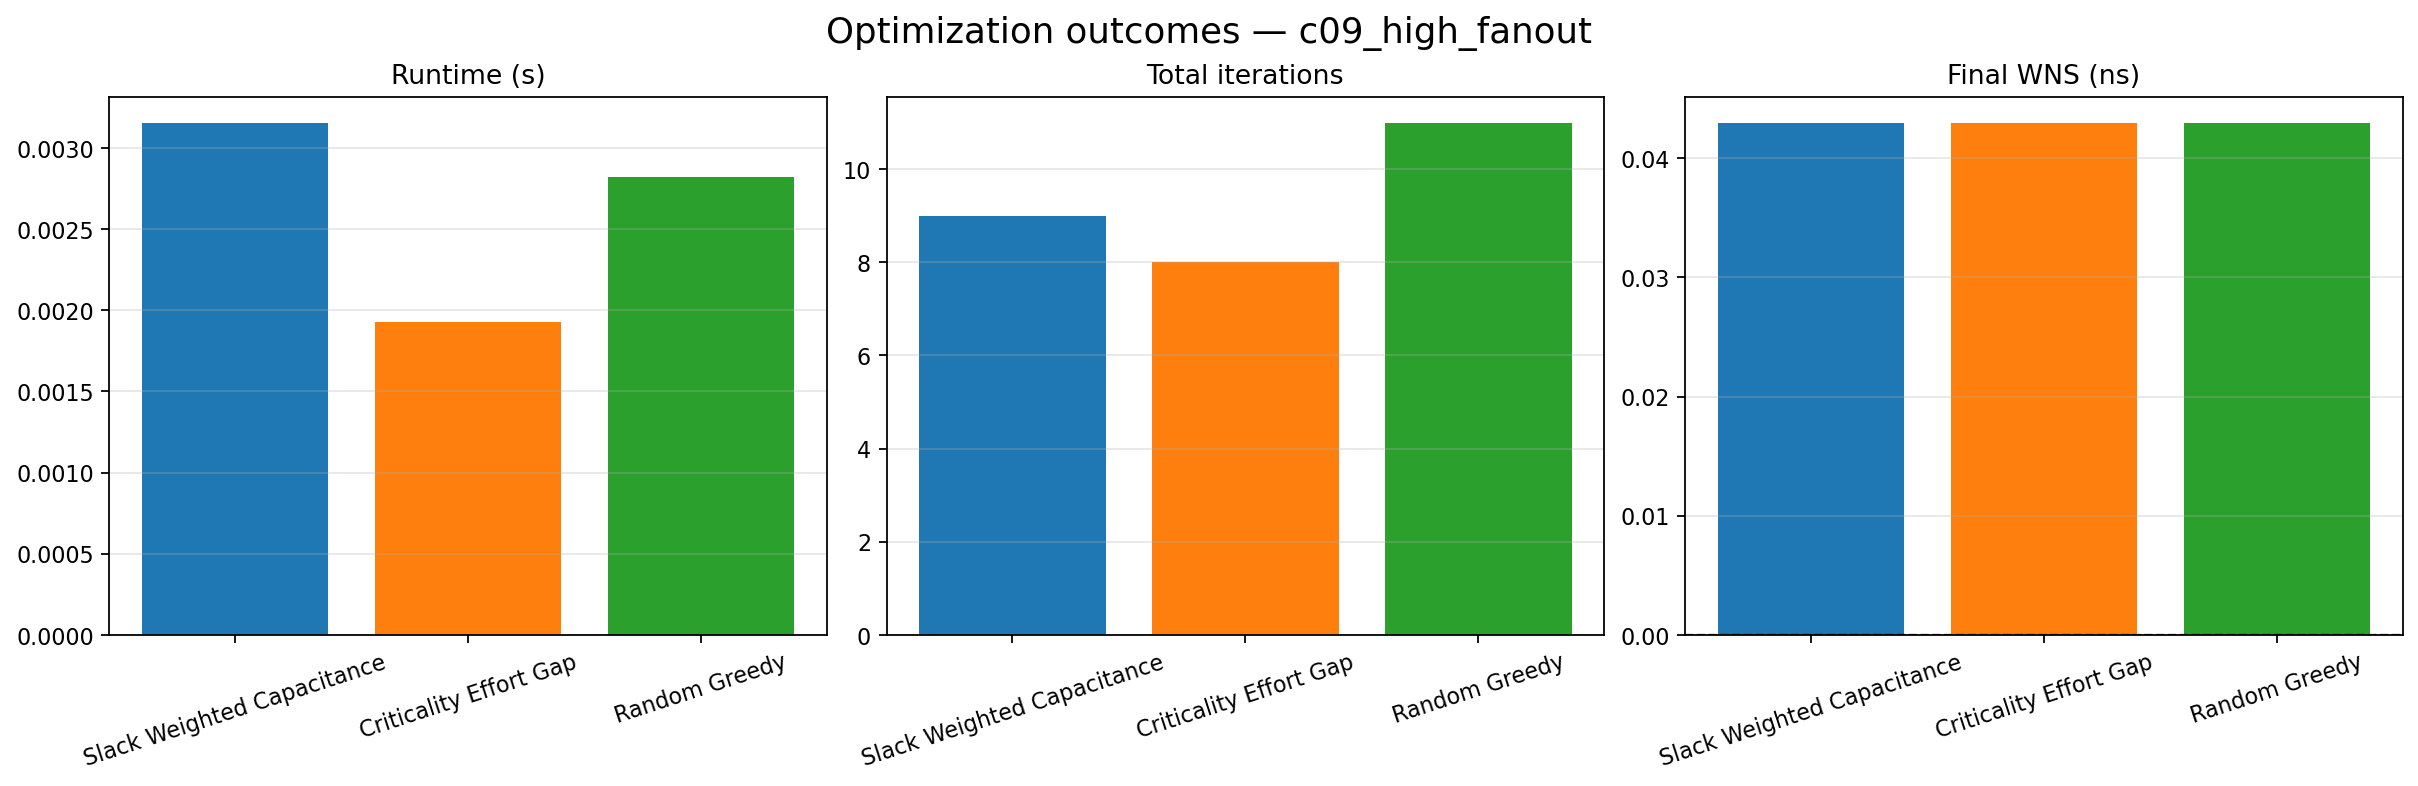
\includegraphics[width=\textwidth]{c09_high_fanout_outc.png}
    \caption{\texttt{c09\_high\_fanout}: optimization outcomes summary.}
    \label{fig:app-c09-high-fanout-outc}
\end{figure}

\clearpage

\section{\texttt{c10\_three\_input\_gates} (5 gates)}
\label{app:fig-c10-three-input-gates}

\begin{figure}[H]
    \centering
    \begin{subfigure}[t]{0.48\textwidth}
        \centering
        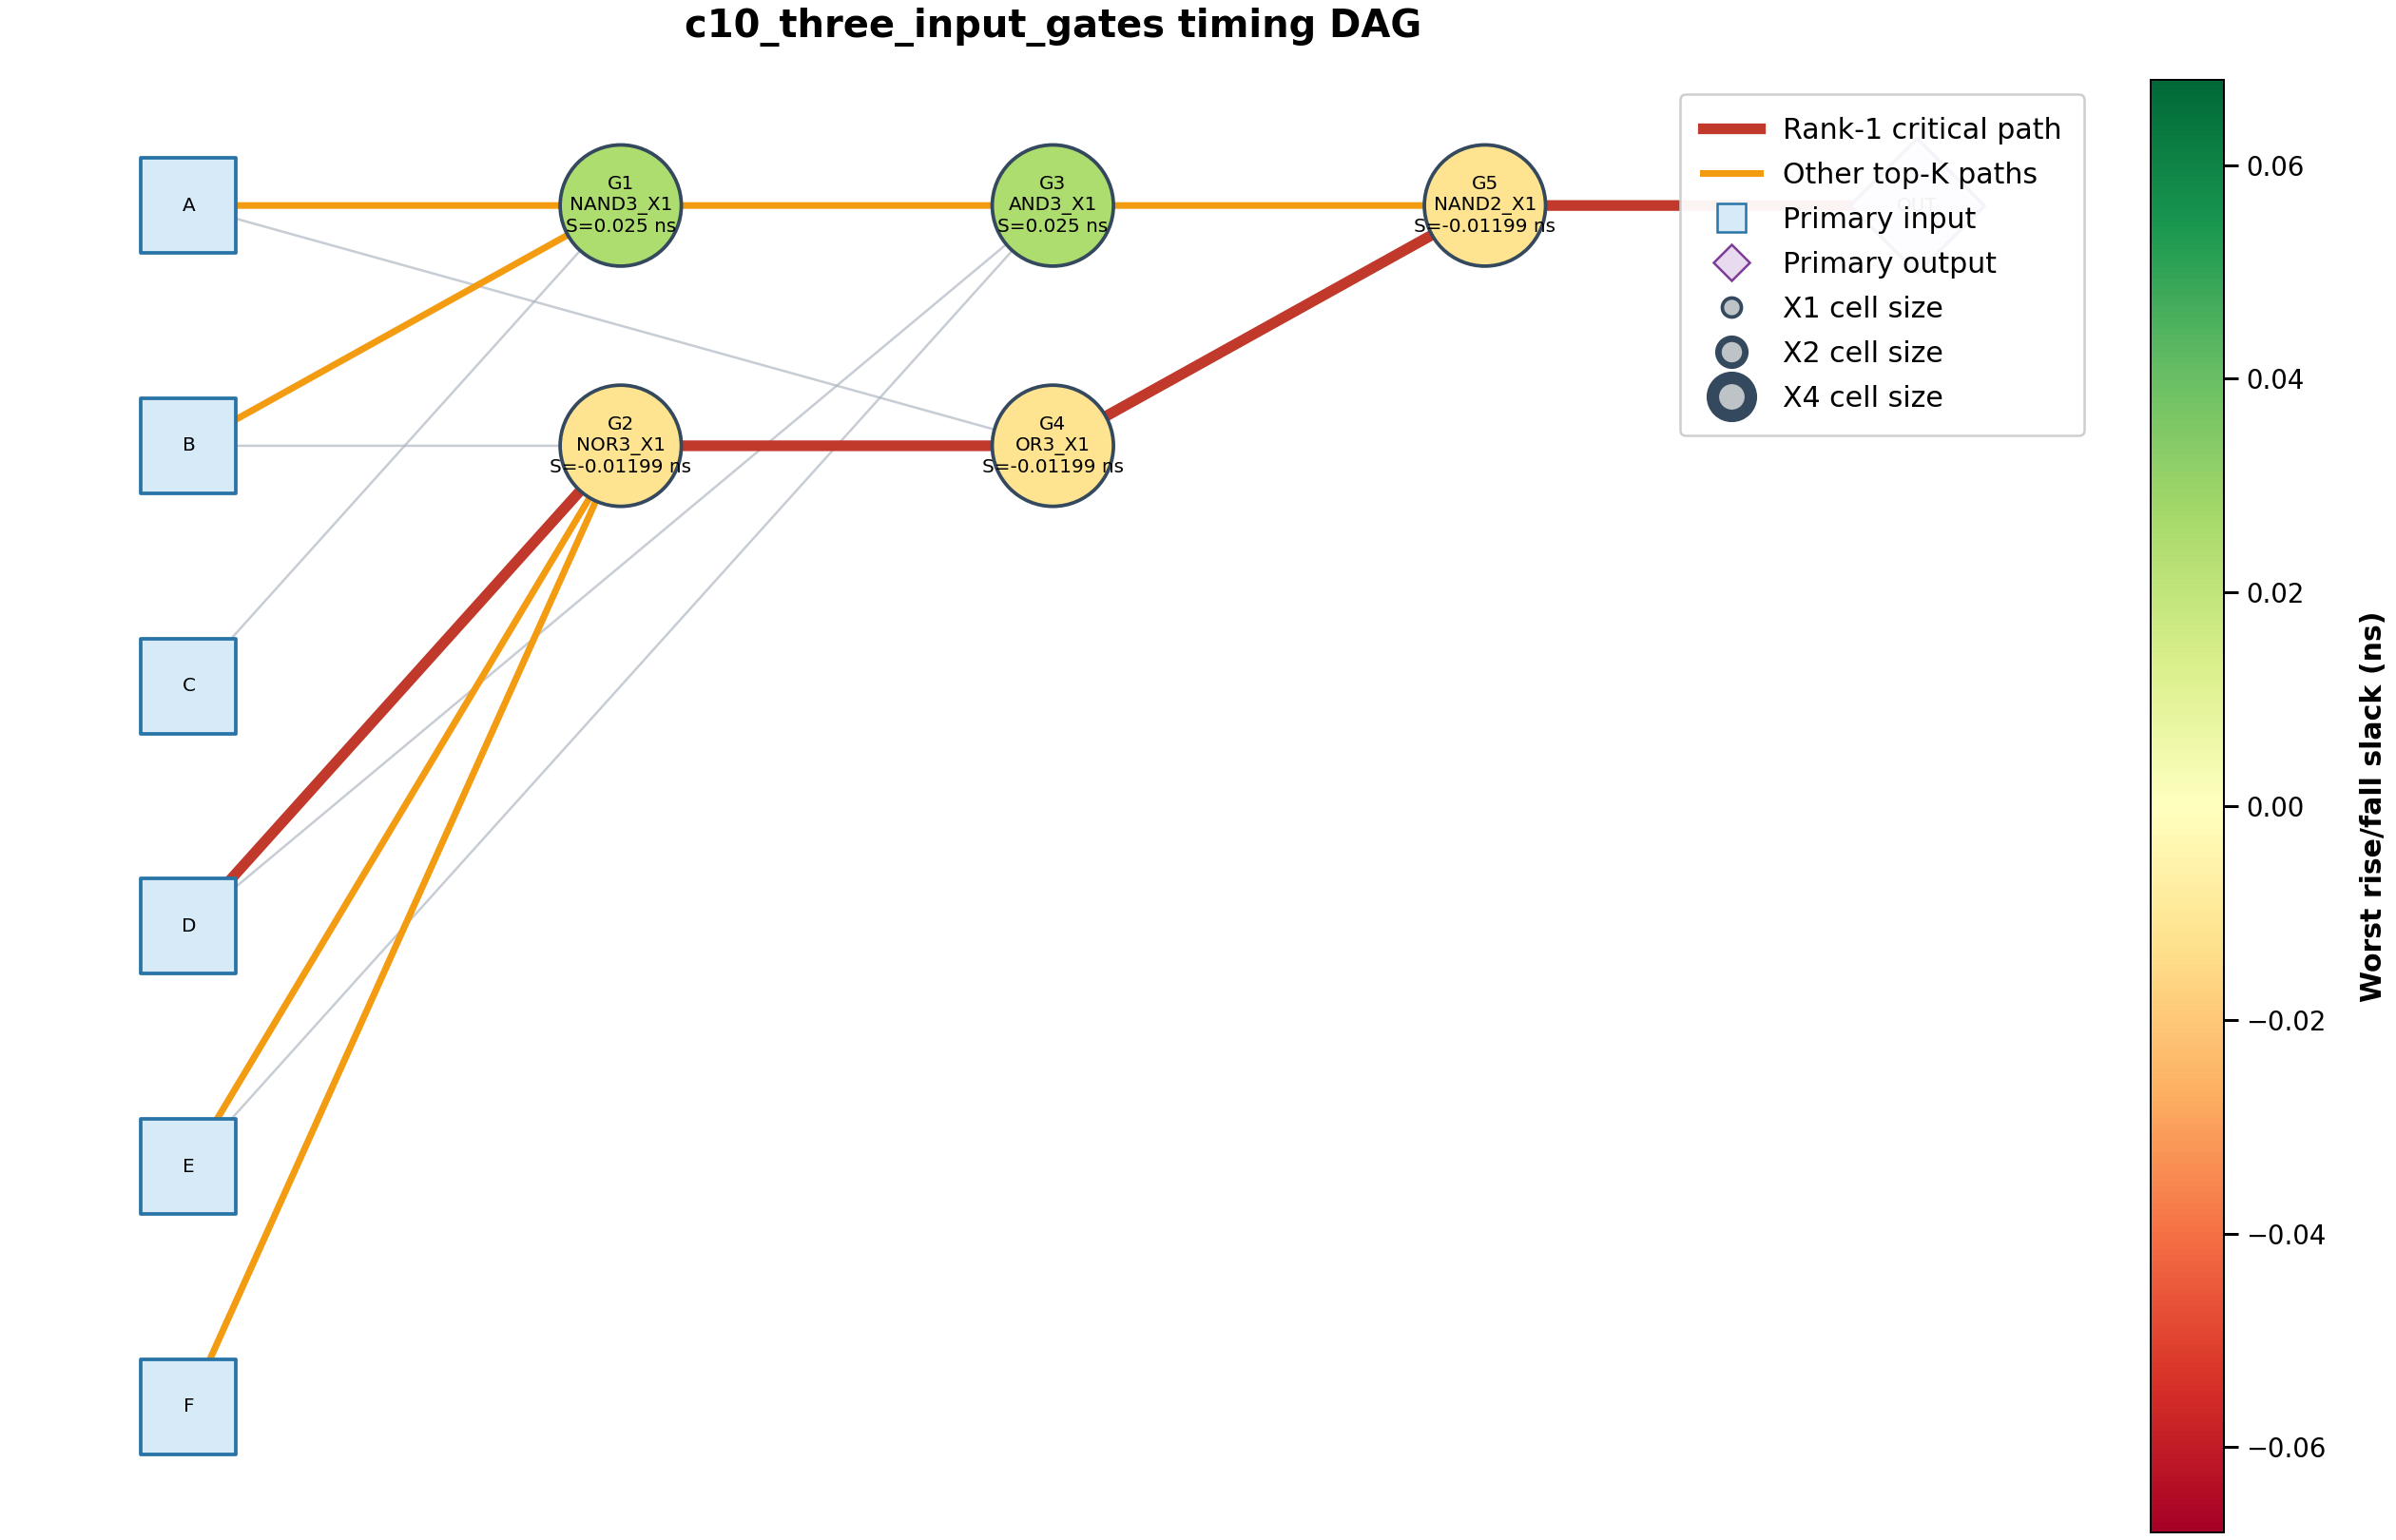
\includegraphics[width=\textwidth]{c10_three_input_gates_pre.png}
        \caption{Pre-optimization}
    \end{subfigure}
    \hfill
    \begin{subfigure}[t]{0.48\textwidth}
        \centering
        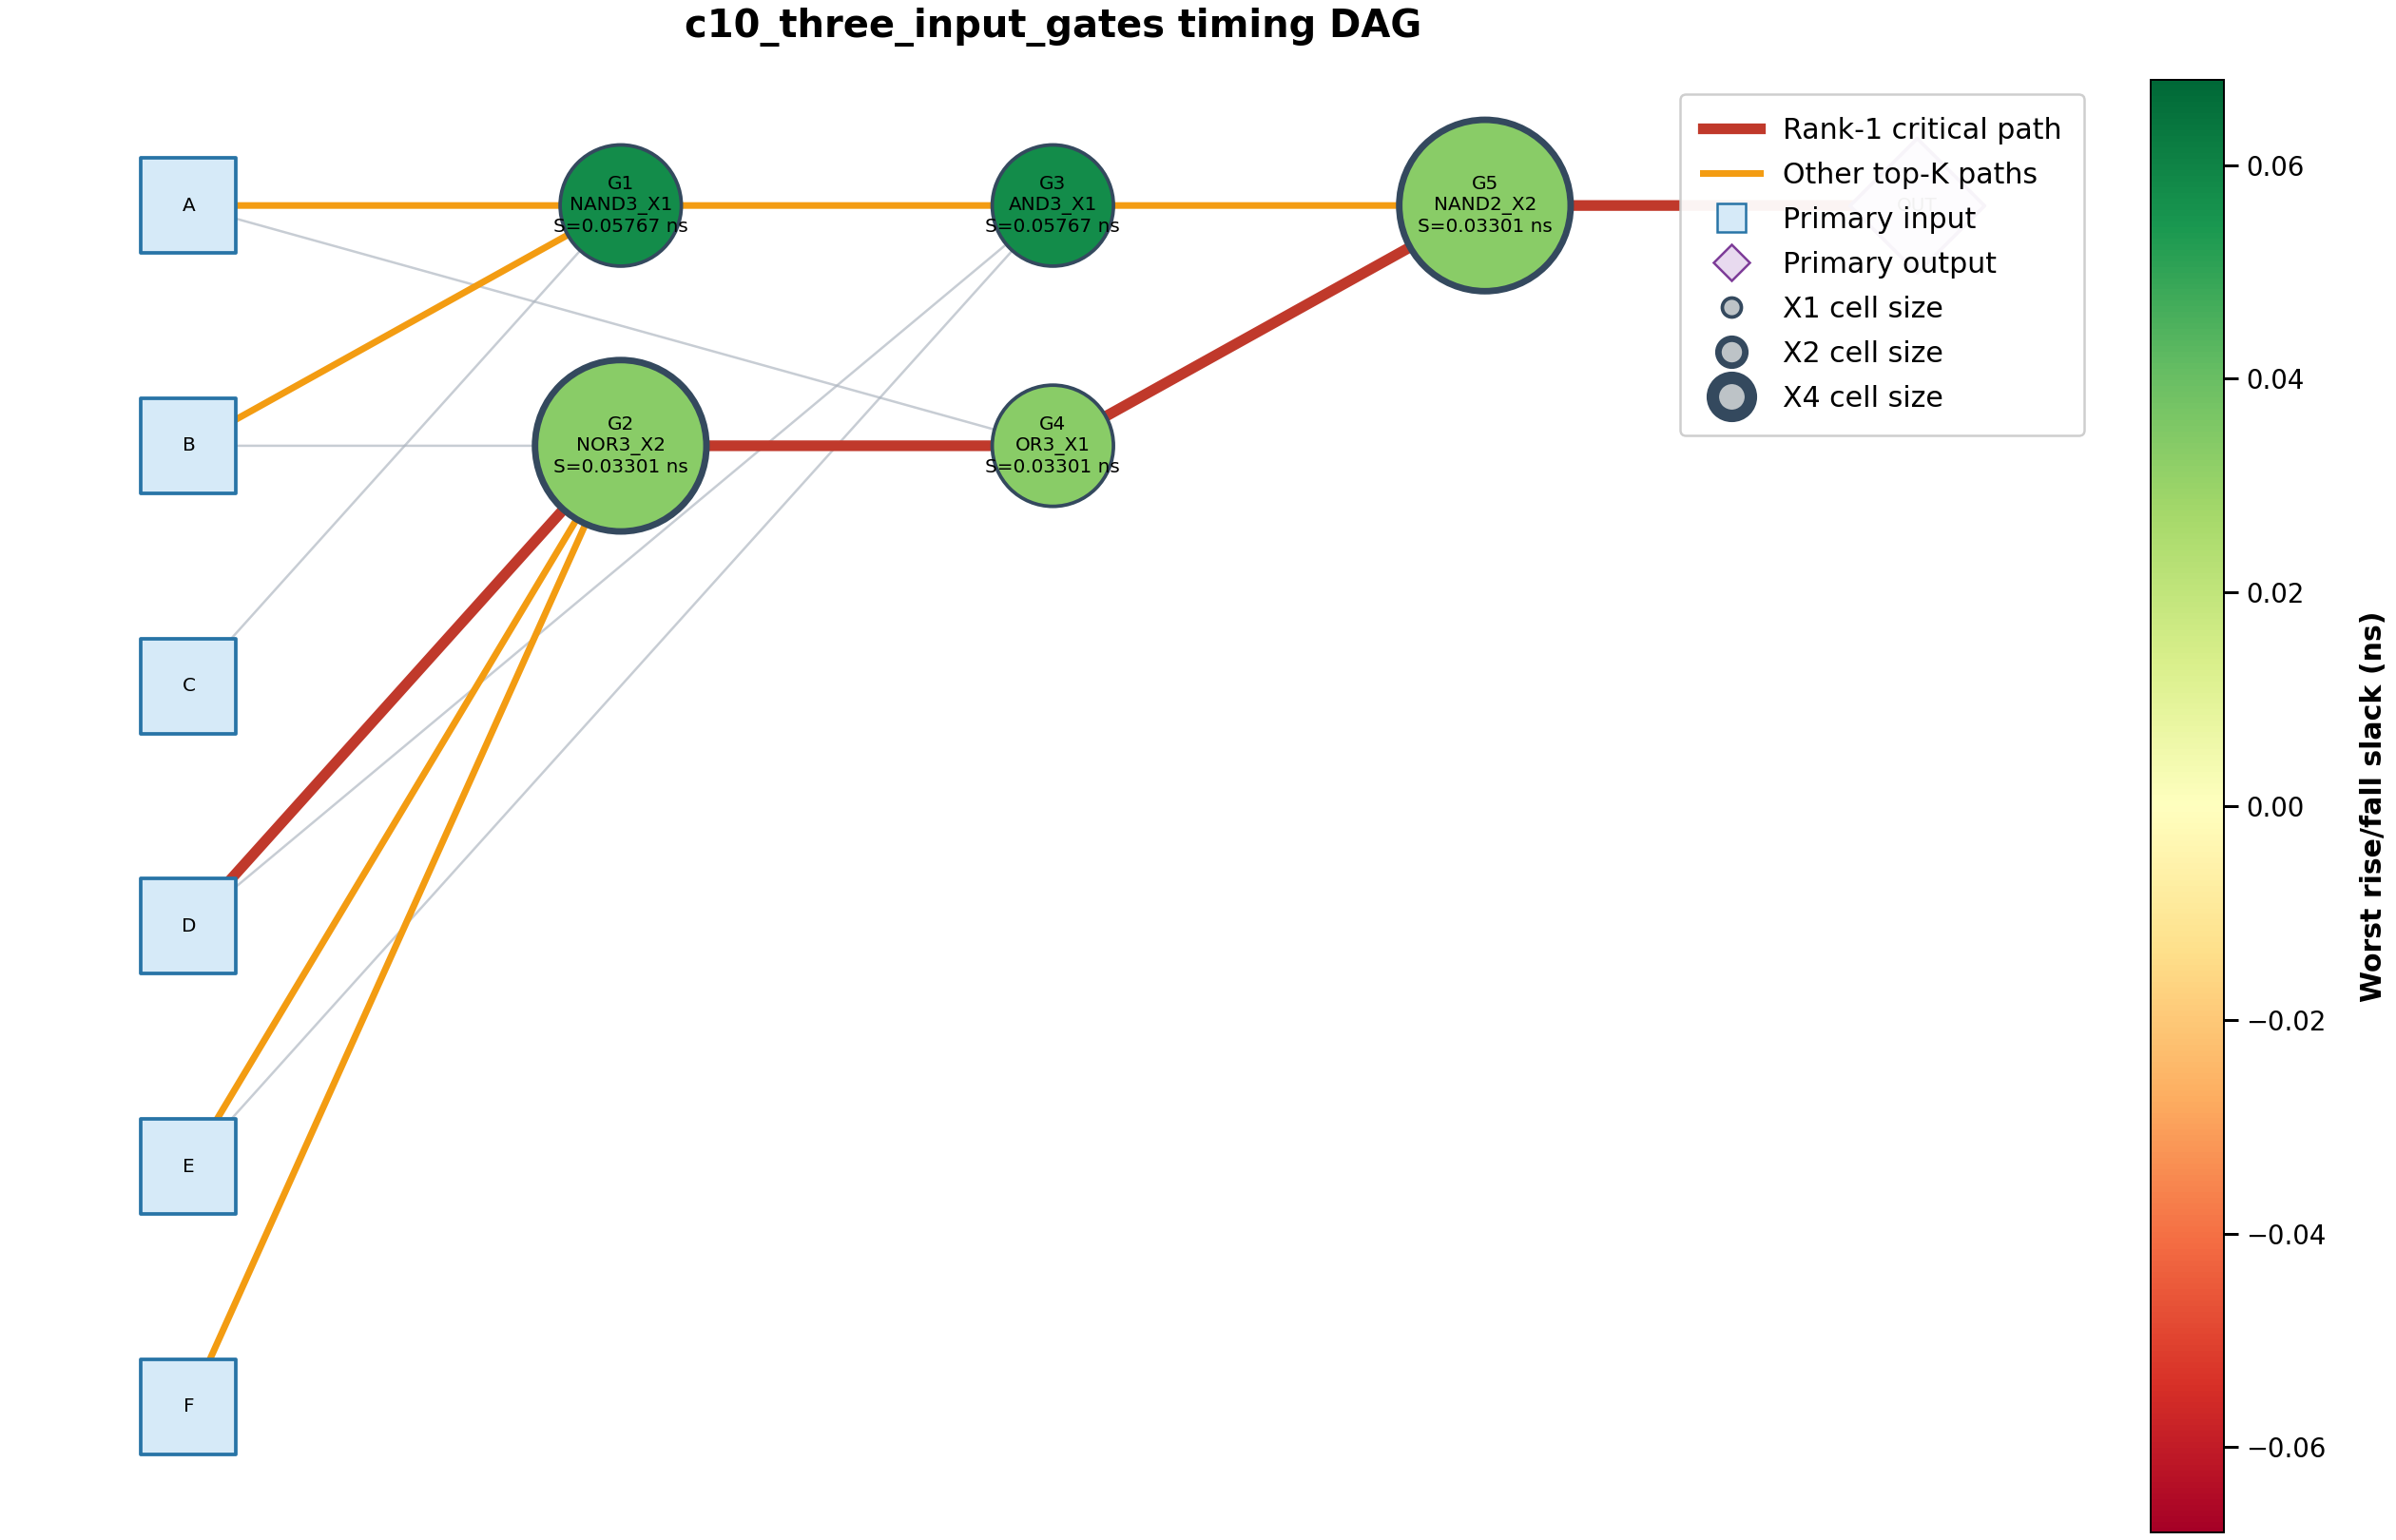
\includegraphics[width=\textwidth]{c10_three_input_gates_post.png}
        \caption{Post-optimization}
    \end{subfigure}
    \caption{\texttt{c10\_three\_input\_gates}: circuit diagrams, nodes colored by slack,
    critical path highlighted.}
    \label{fig:app-c10-three-input-gates-graphs}
\end{figure}

\begin{figure}[H]
    \centering
    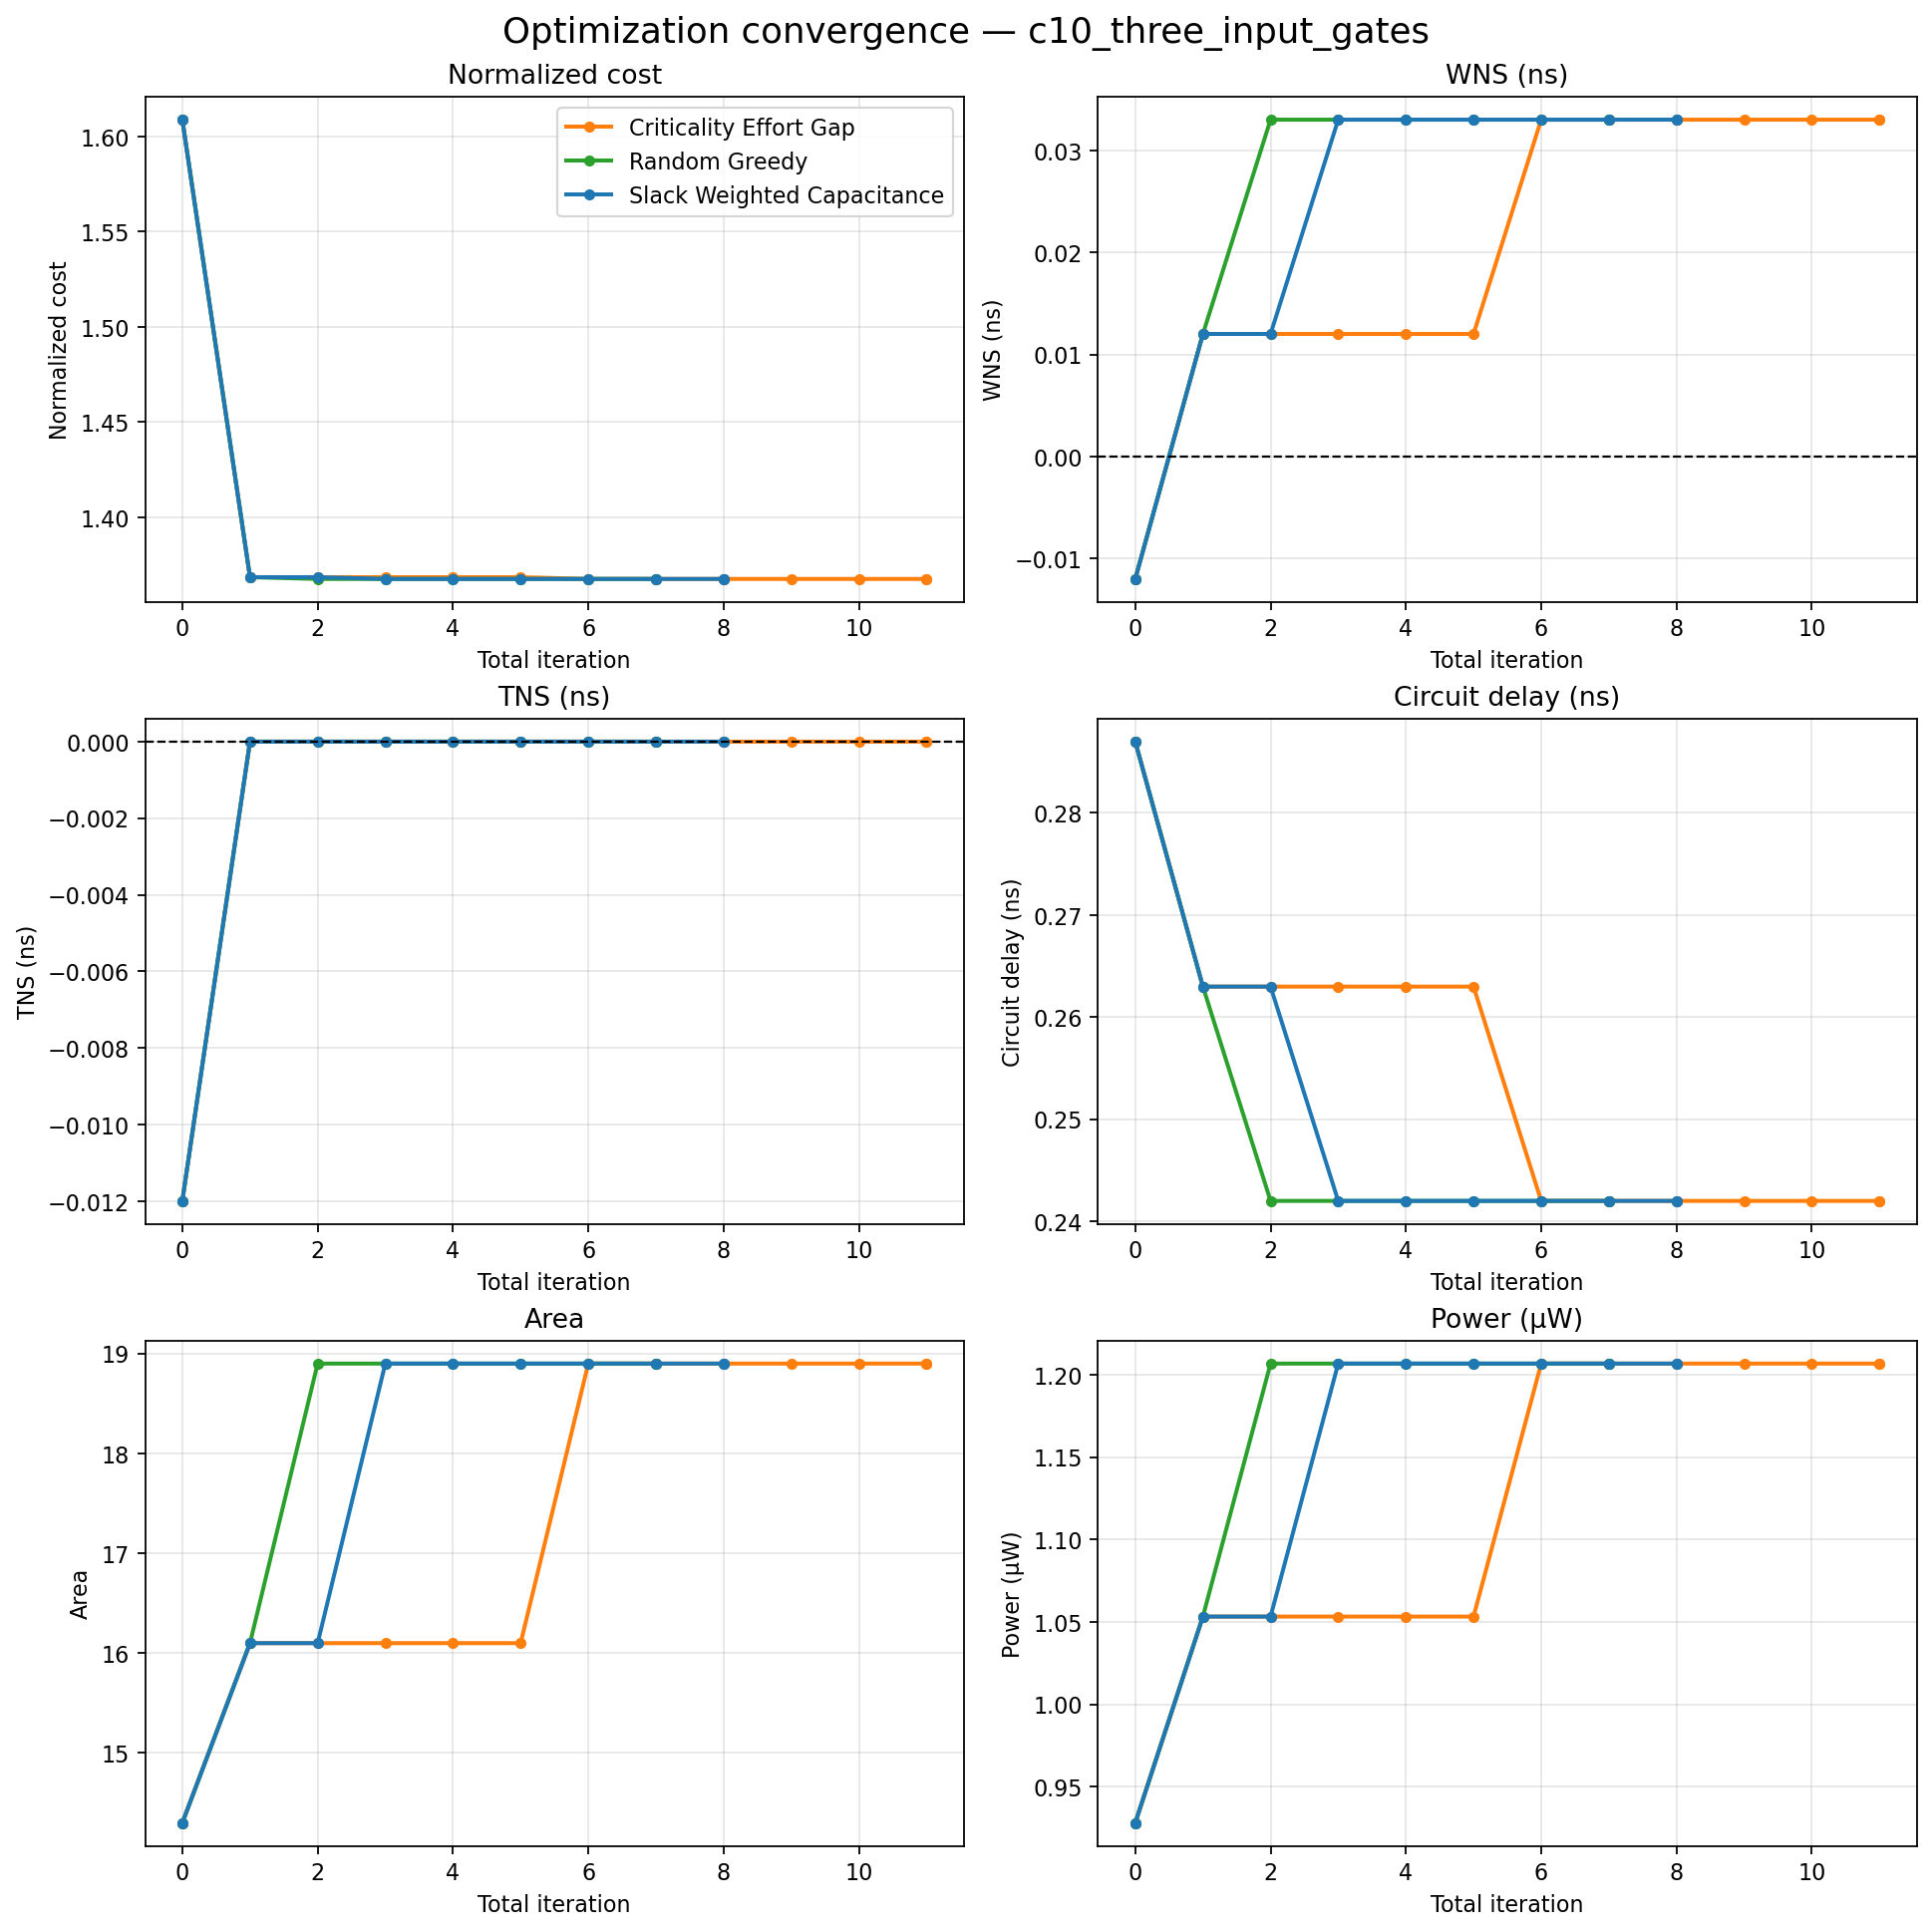
\includegraphics[width=\textwidth]{c10_three_input_gates_conv.png}
    \caption{\texttt{c10\_three\_input\_gates}: optimization convergence trace.}
    \label{fig:app-c10-three-input-gates-conv}
\end{figure}

\begin{figure}[H]
    \centering
    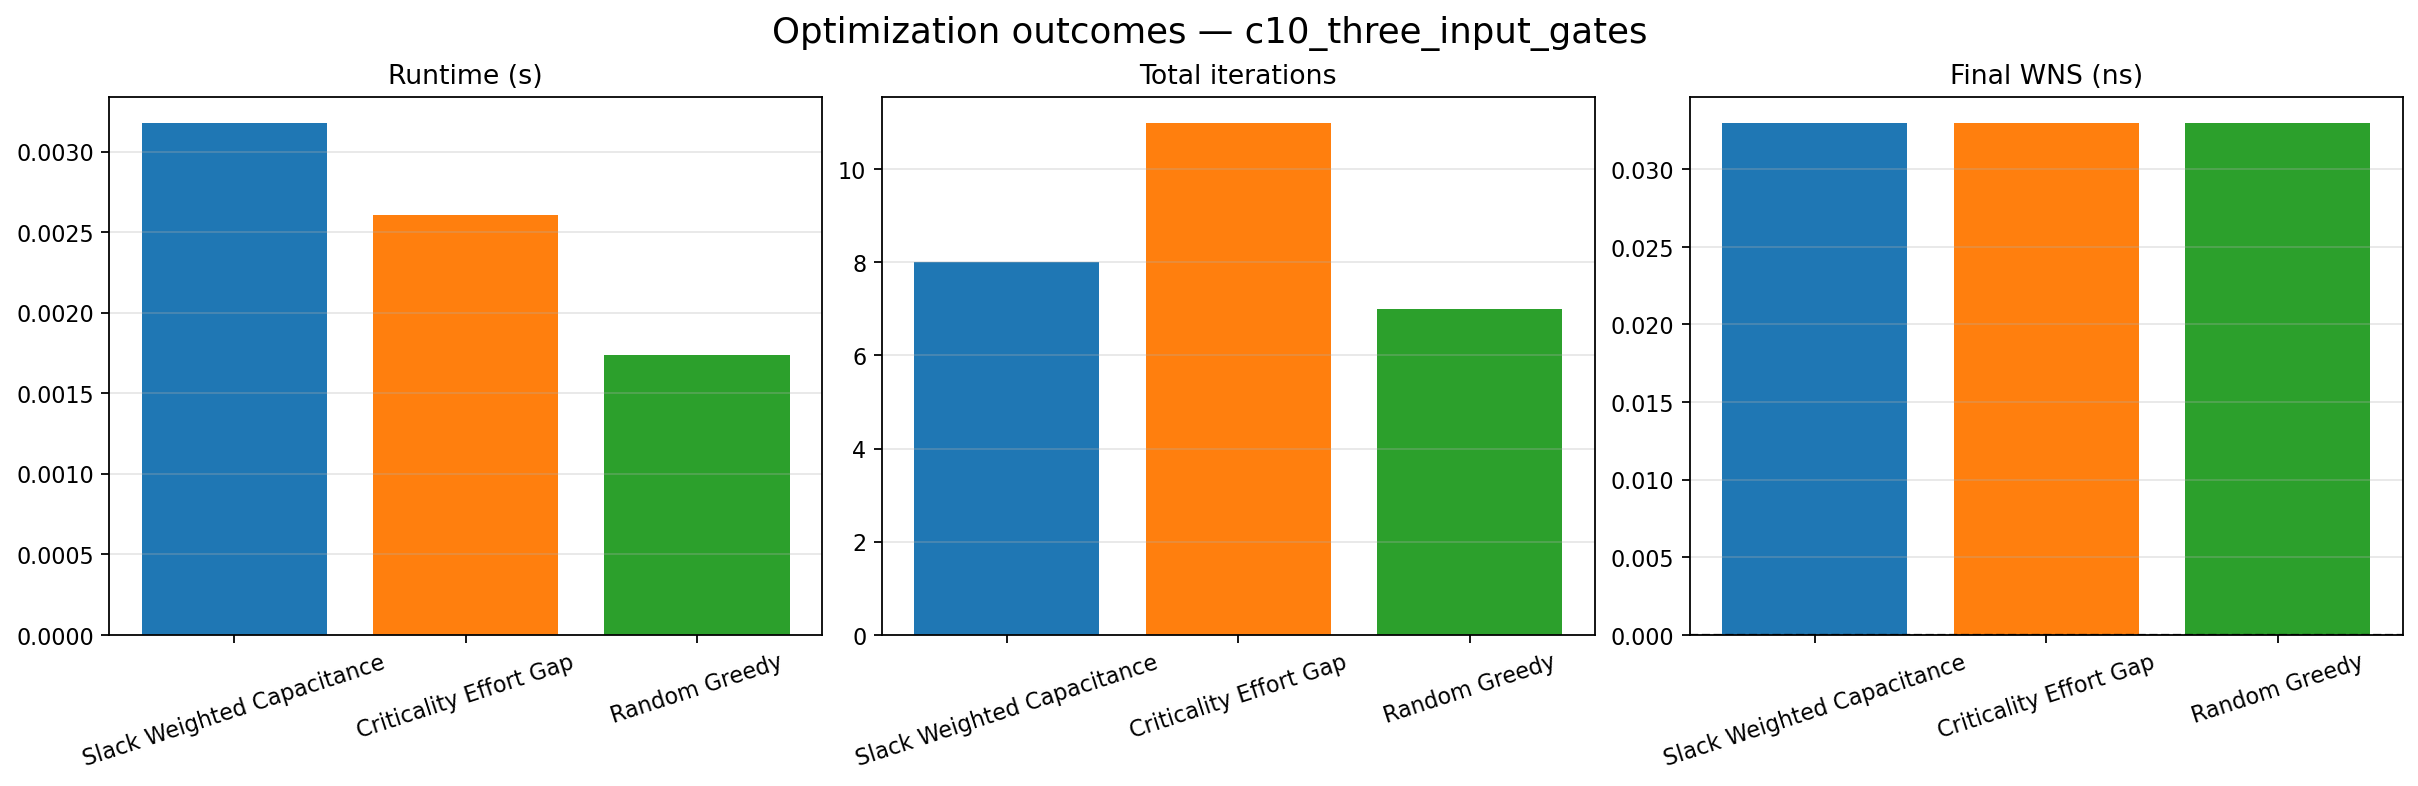
\includegraphics[width=\textwidth]{c10_three_input_gates_outc.png}
    \caption{\texttt{c10\_three\_input\_gates}: optimization outcomes summary.}
    \label{fig:app-c10-three-input-gates-outc}
\end{figure}

\clearpage

\section{\texttt{c11\_gate\_sizing\_stress} (6 gates)}
\label{app:fig-c11-gate-sizing-stress}

\begin{figure}[H]
    \centering
    \begin{subfigure}[t]{0.48\textwidth}
        \centering
        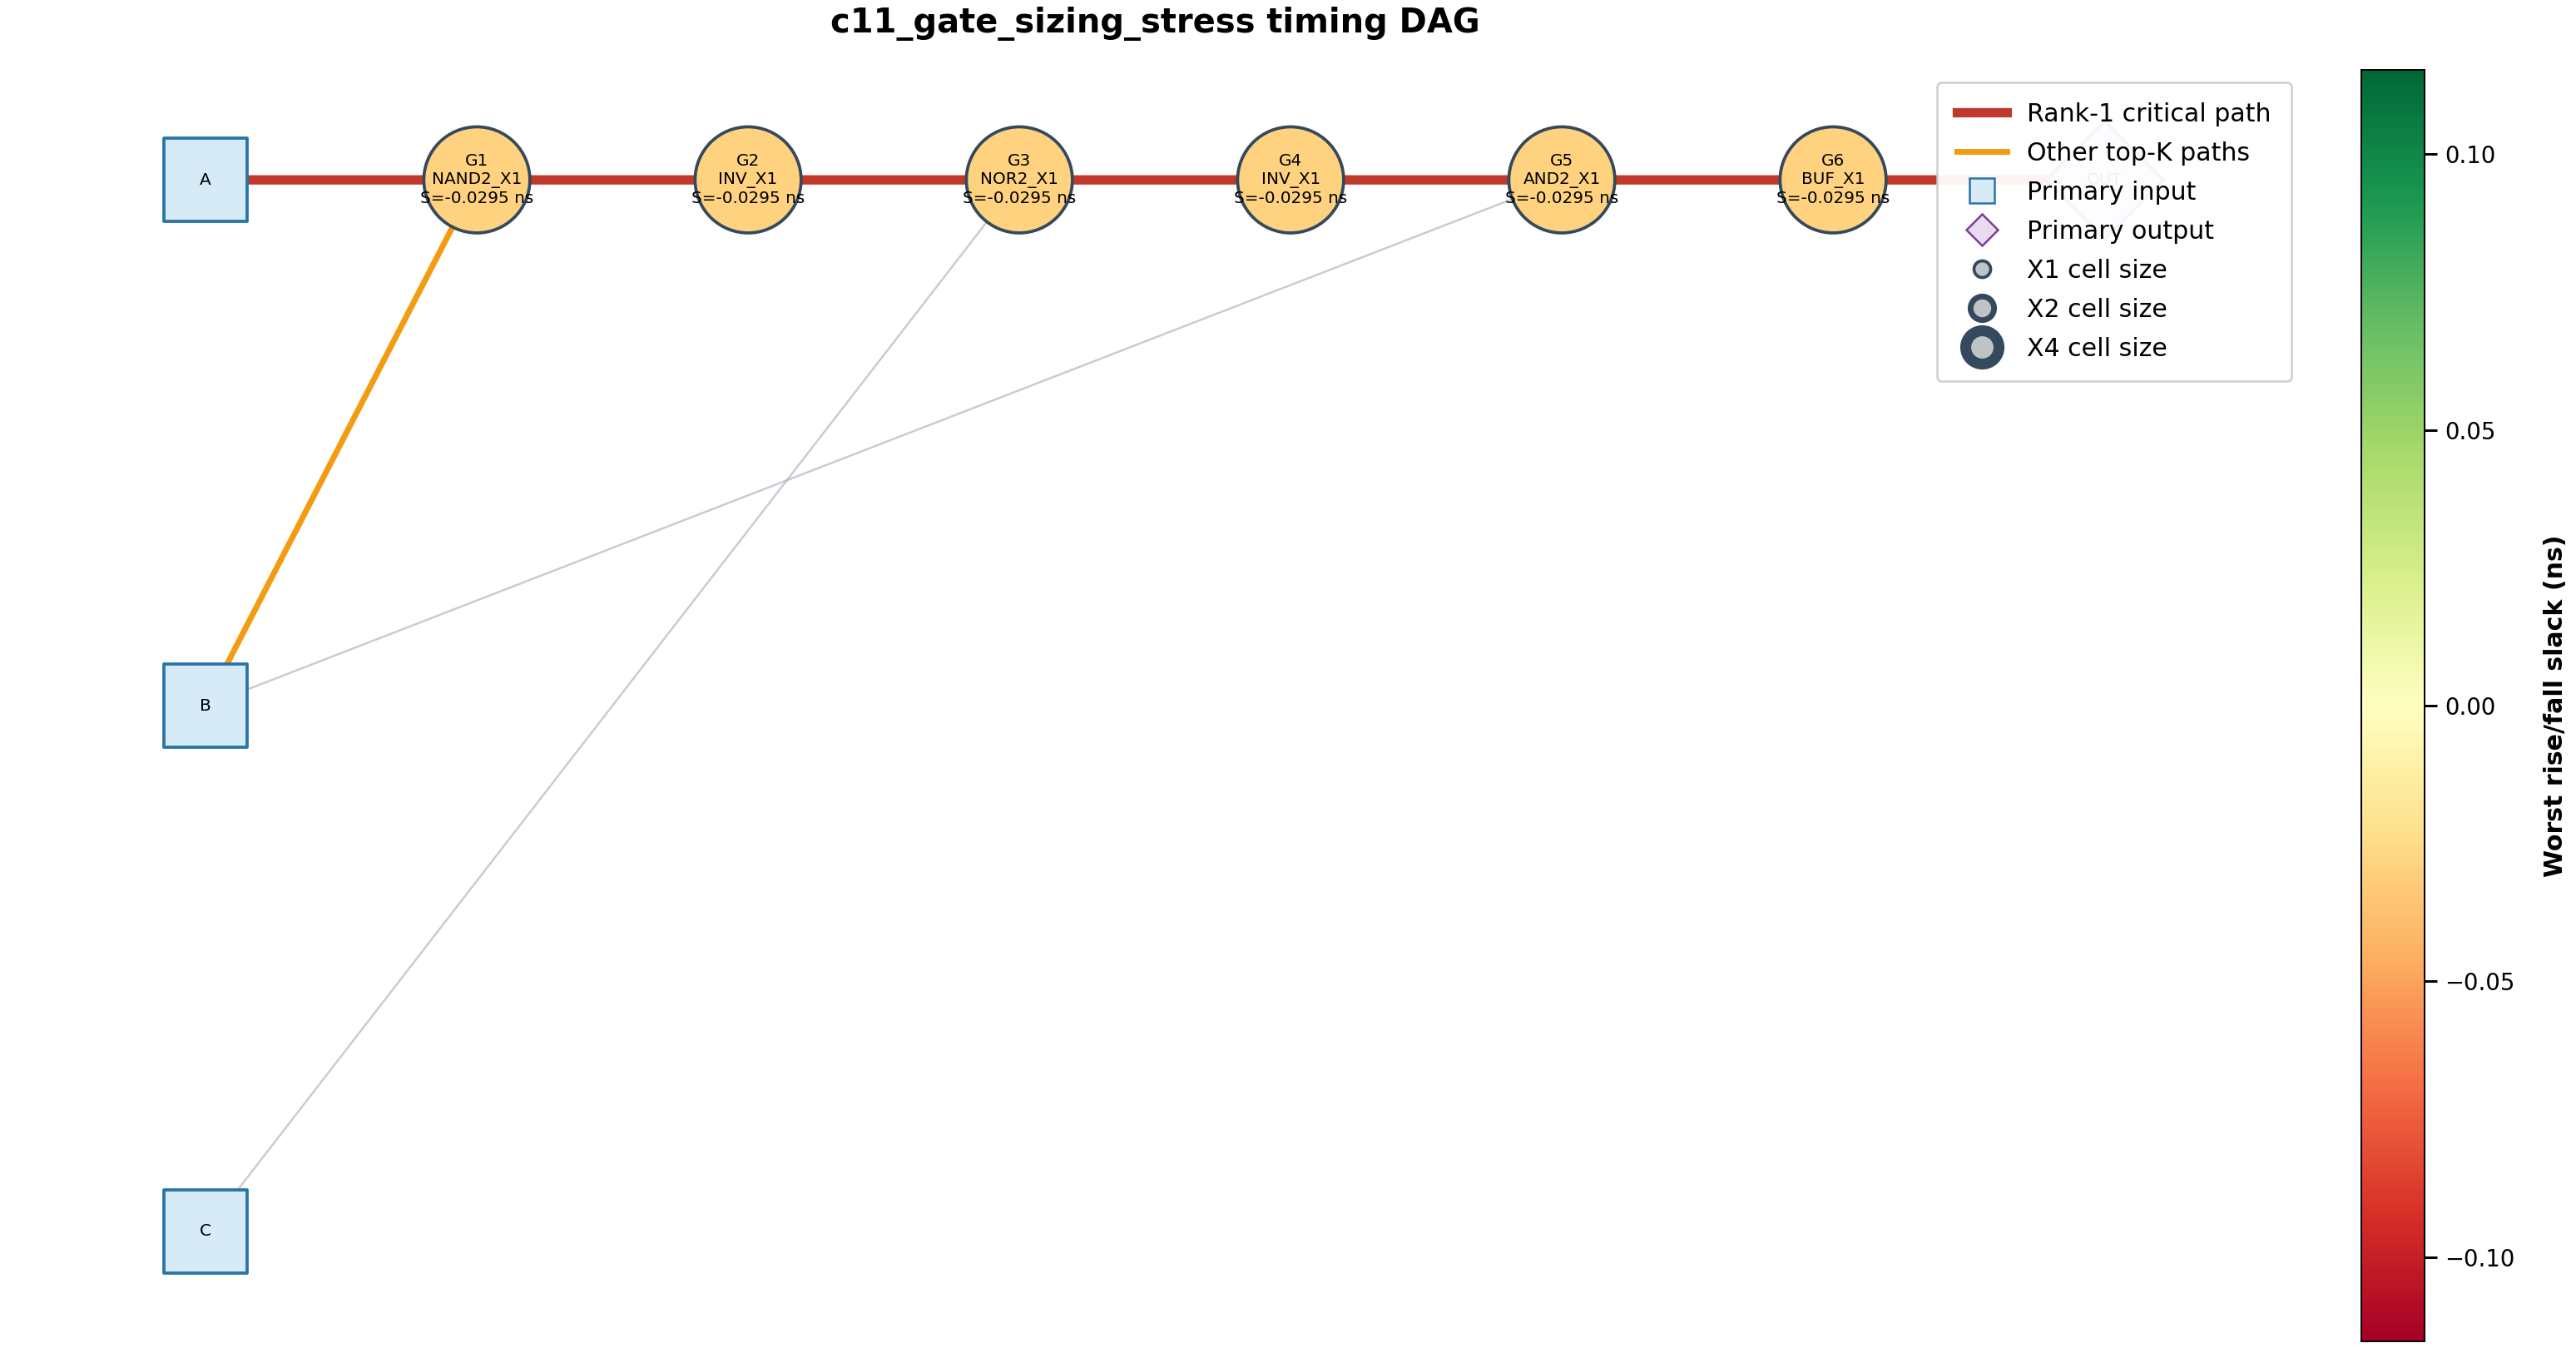
\includegraphics[width=\textwidth]{c11_gate_sizing_stress_pre.png}
        \caption{Pre-optimization}
    \end{subfigure}
    \hfill
    \begin{subfigure}[t]{0.48\textwidth}
        \centering
        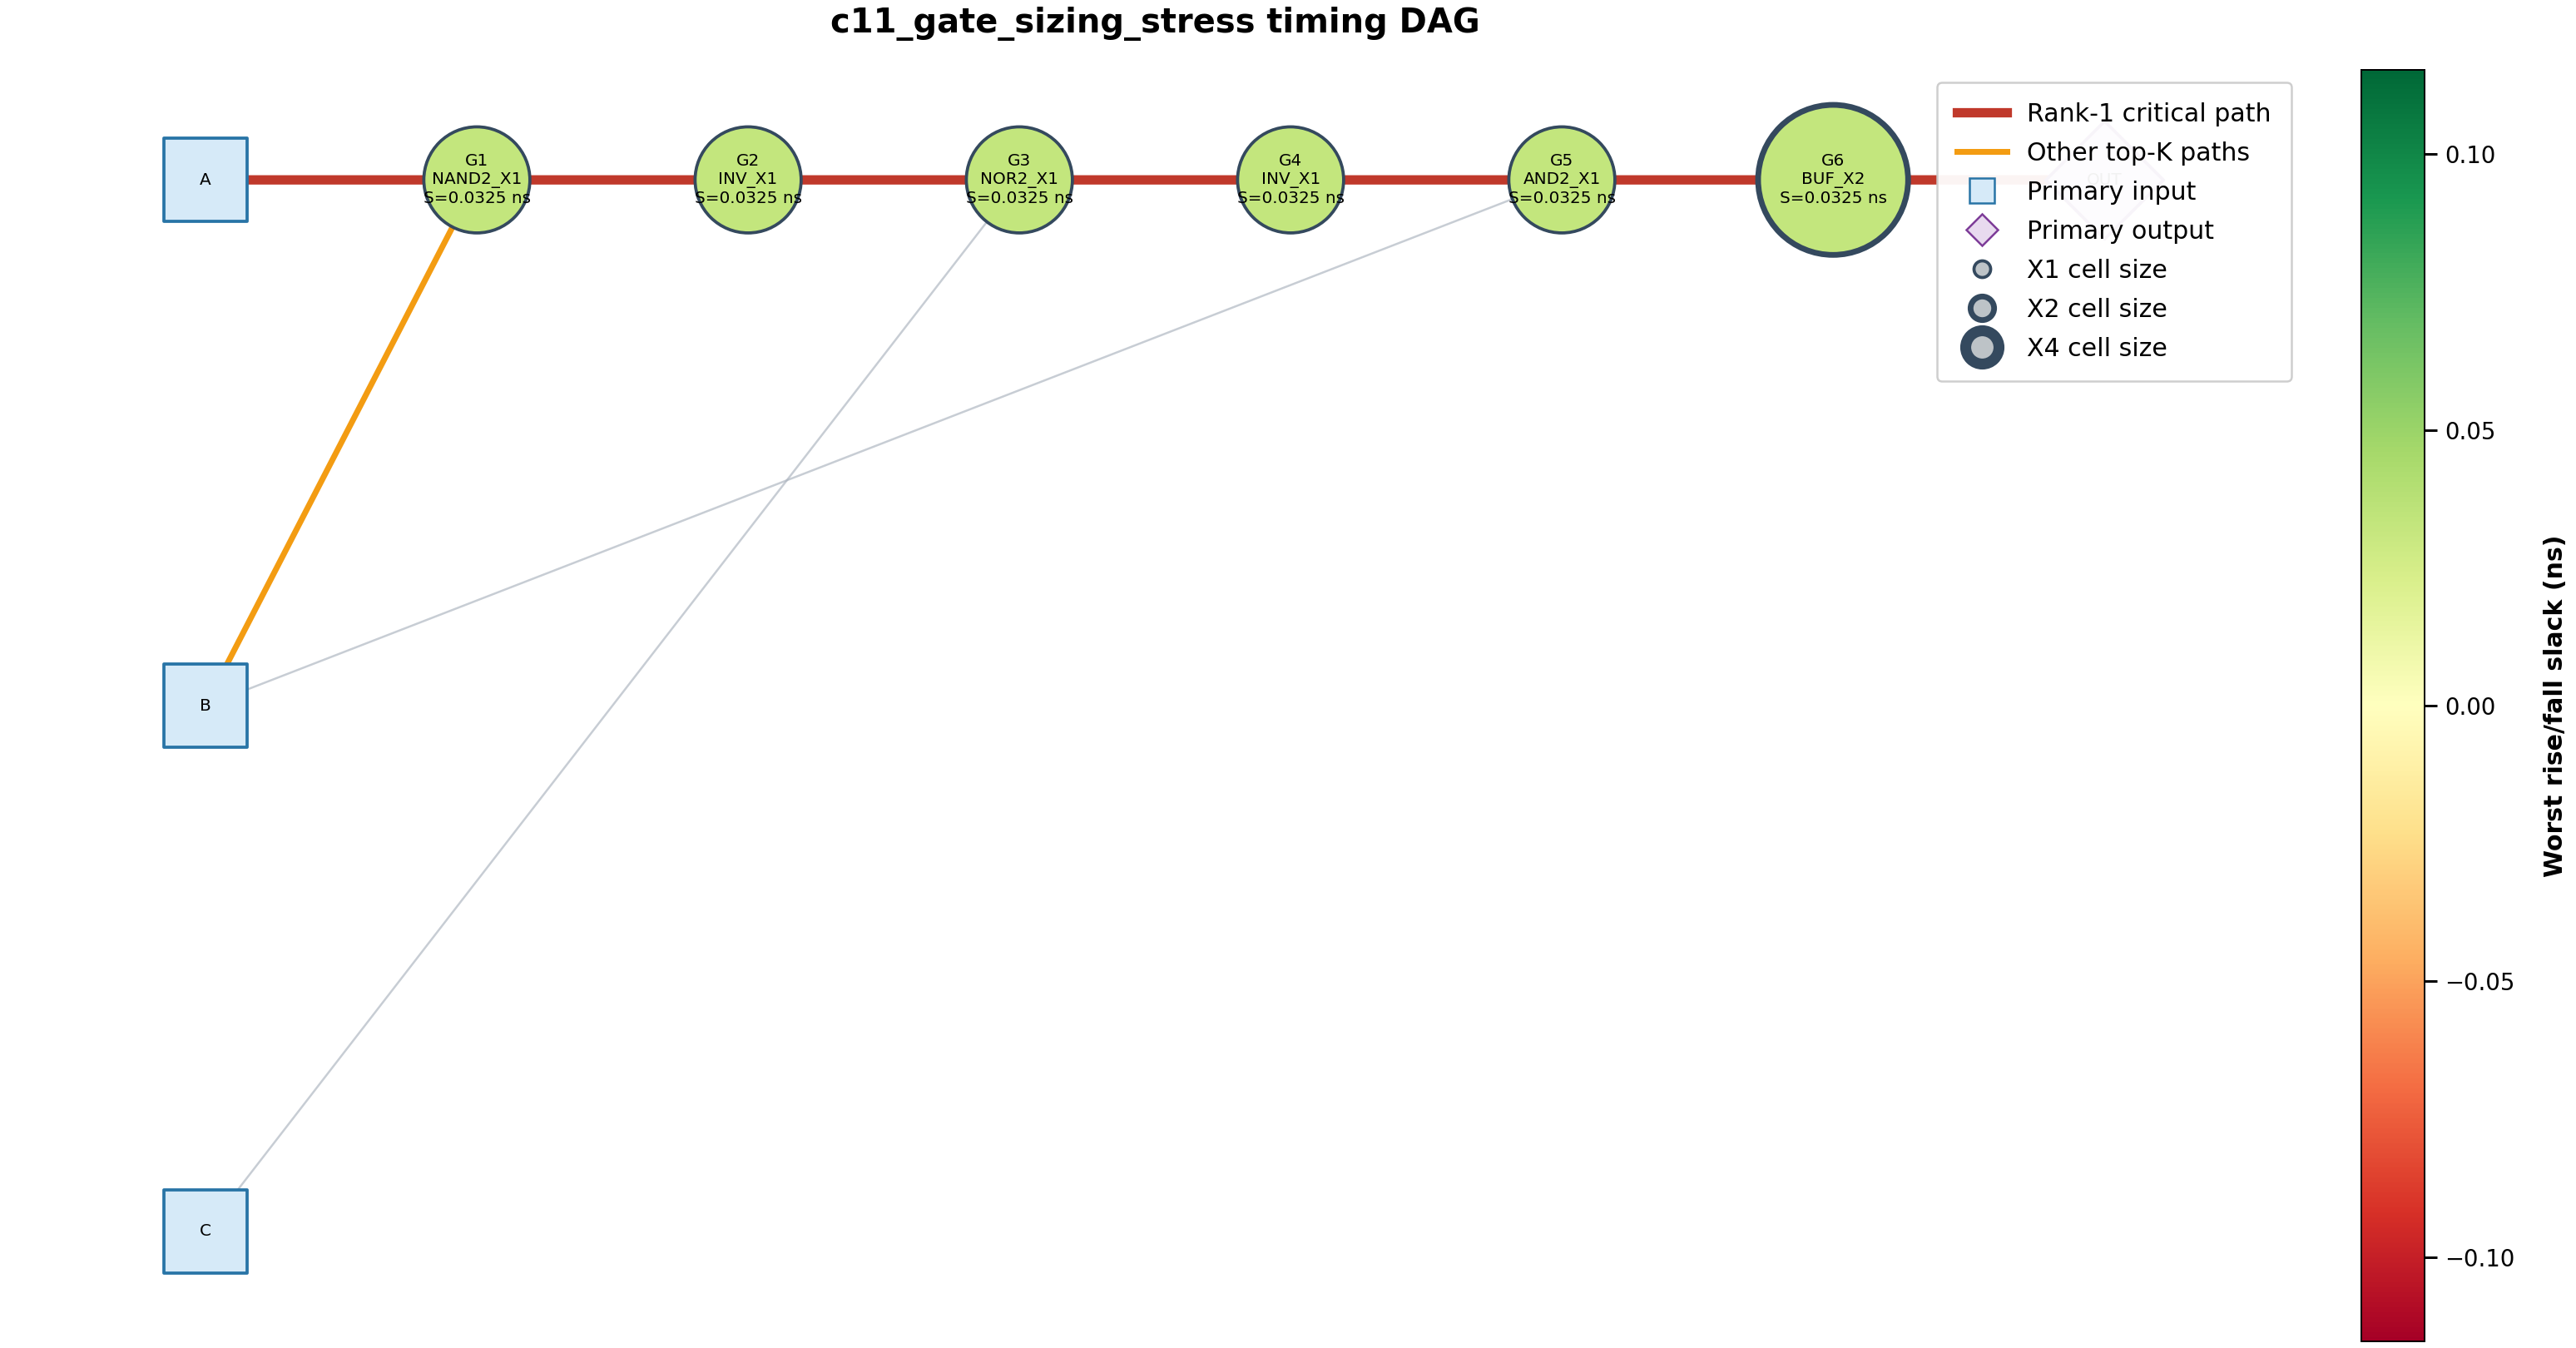
\includegraphics[width=\textwidth]{c11_gate_sizing_stress_post.png}
        \caption{Post-optimization}
    \end{subfigure}
    \caption{\texttt{c11\_gate\_sizing\_stress}: circuit diagrams, nodes colored by slack,
    critical path highlighted.}
    \label{fig:app-c11-gate-sizing-stress-graphs}
\end{figure}

\begin{figure}[H]
    \centering
    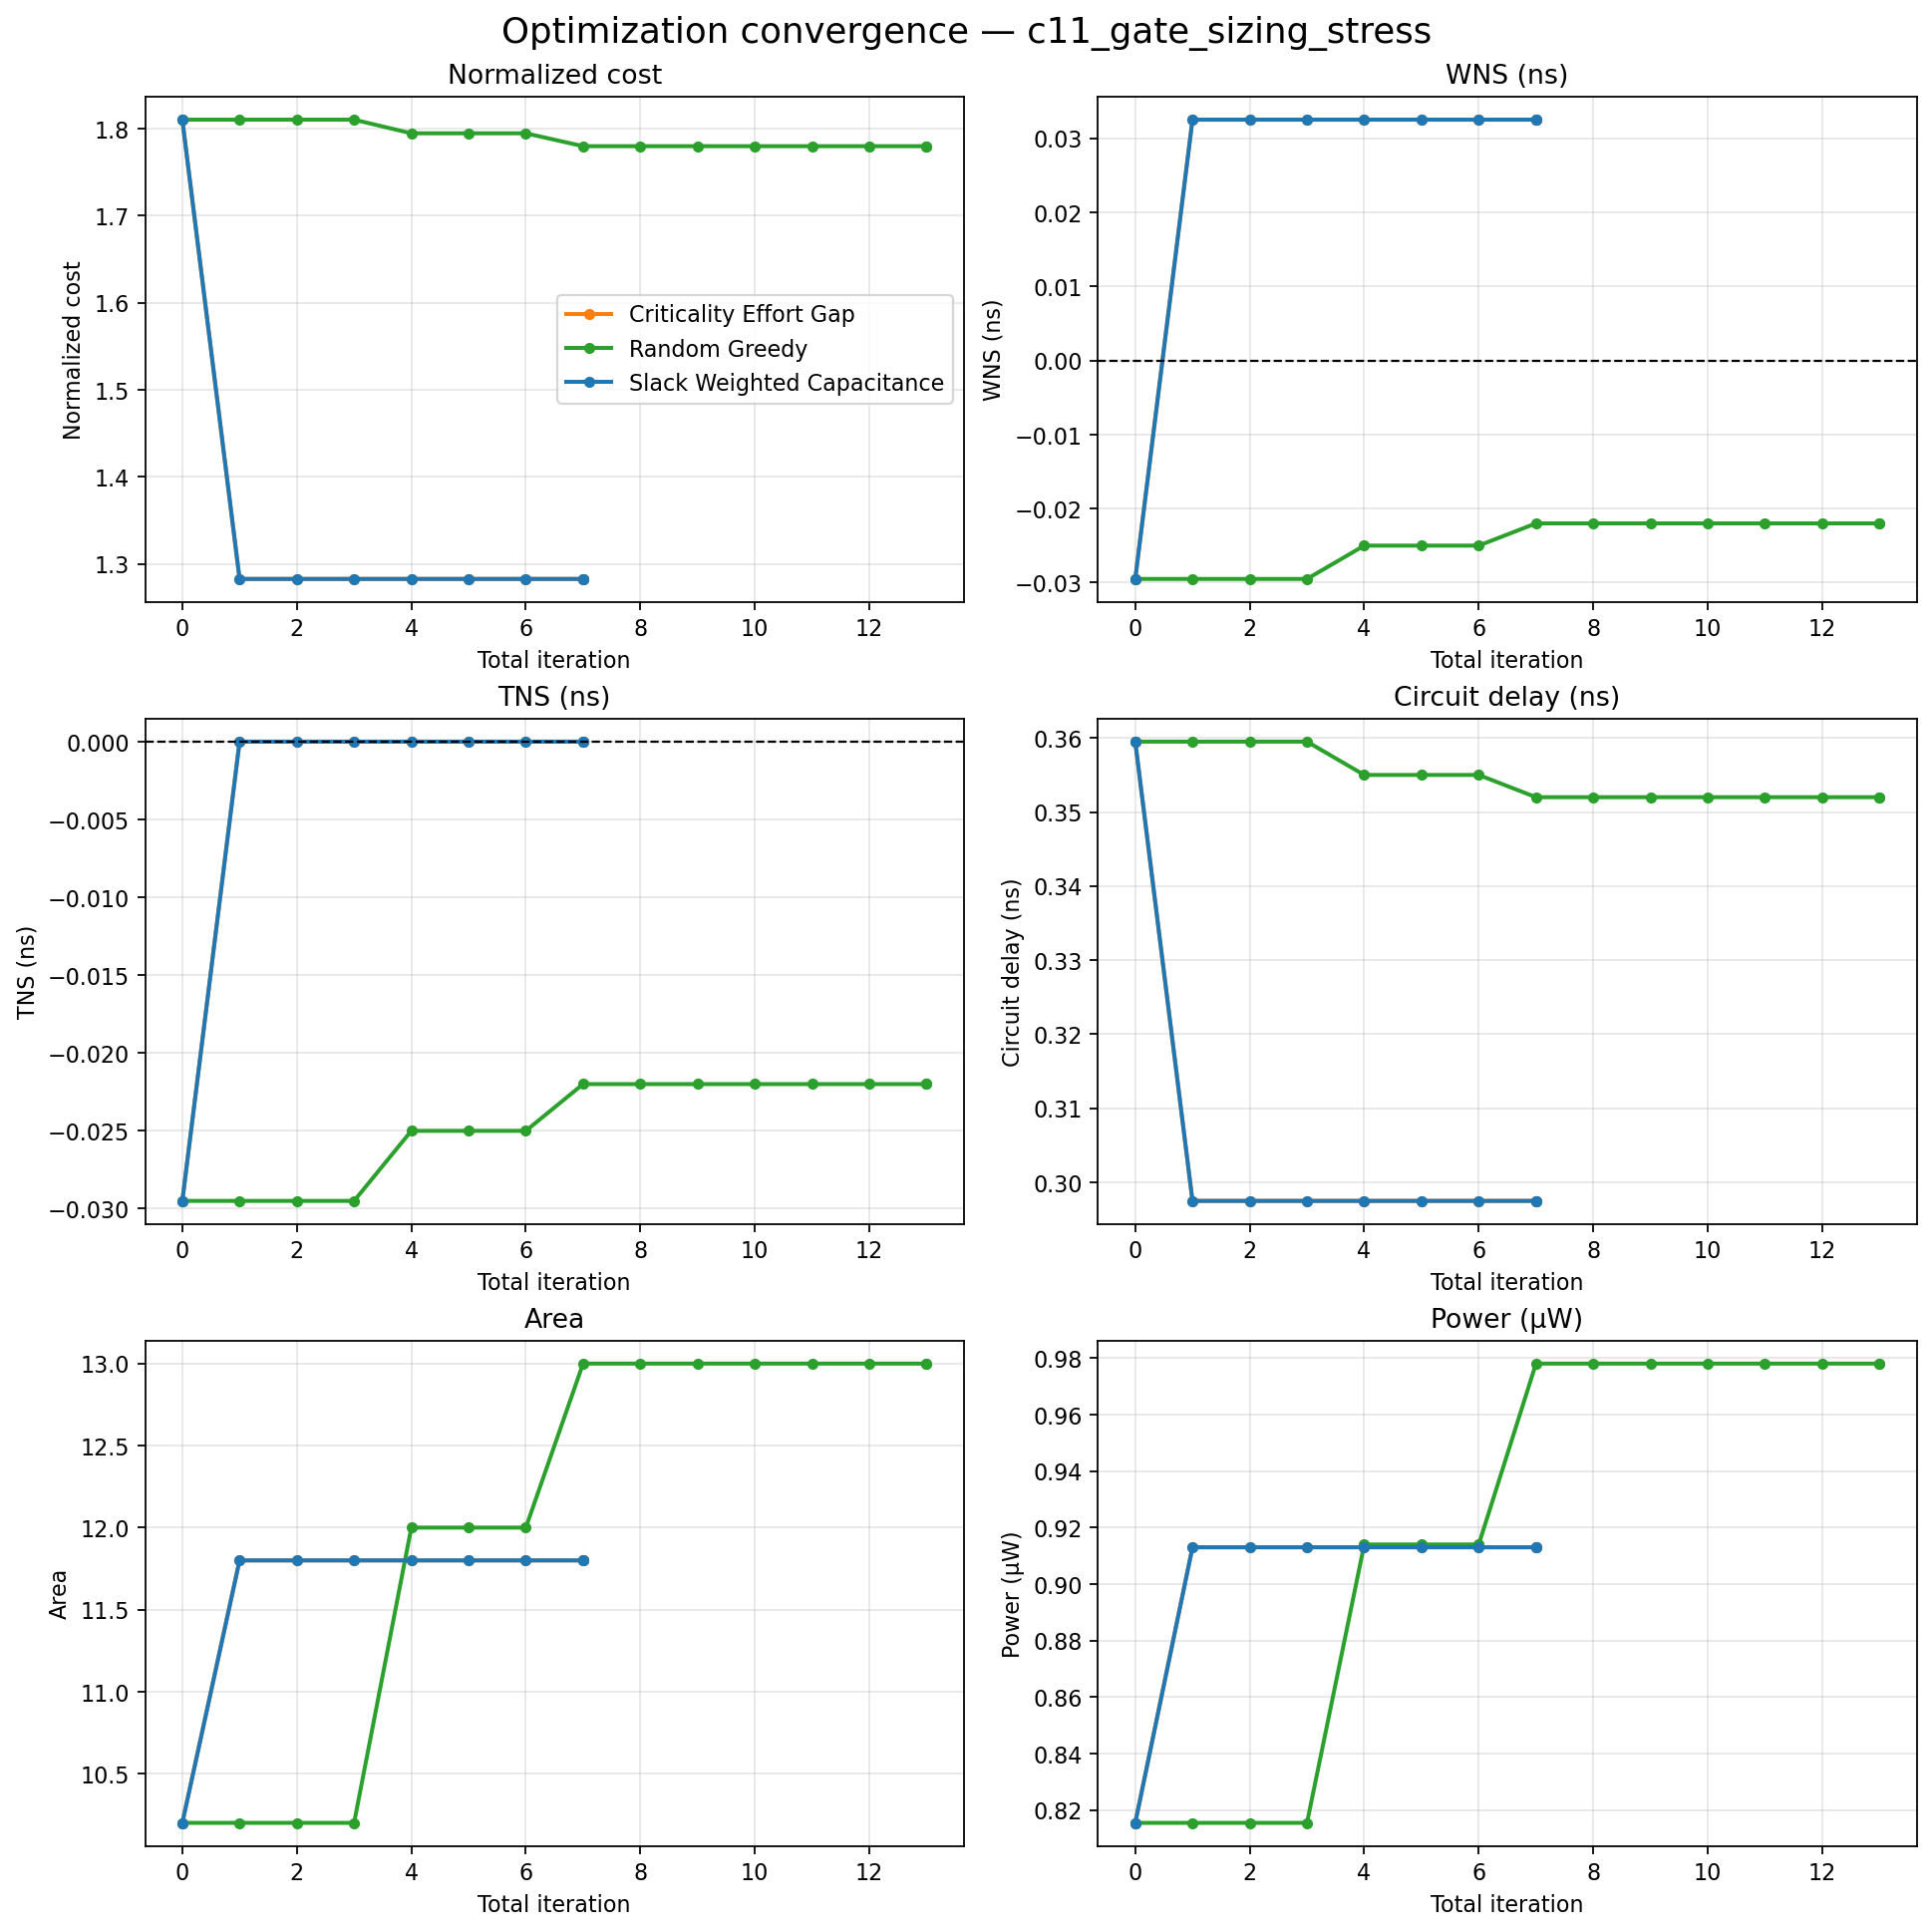
\includegraphics[width=\textwidth]{c11_gate_sizing_stress_conv.png}
    \caption{\texttt{c11\_gate\_sizing\_stress}: optimization convergence trace.}
    \label{fig:app-c11-gate-sizing-stress-conv}
\end{figure}

\begin{figure}[H]
    \centering
    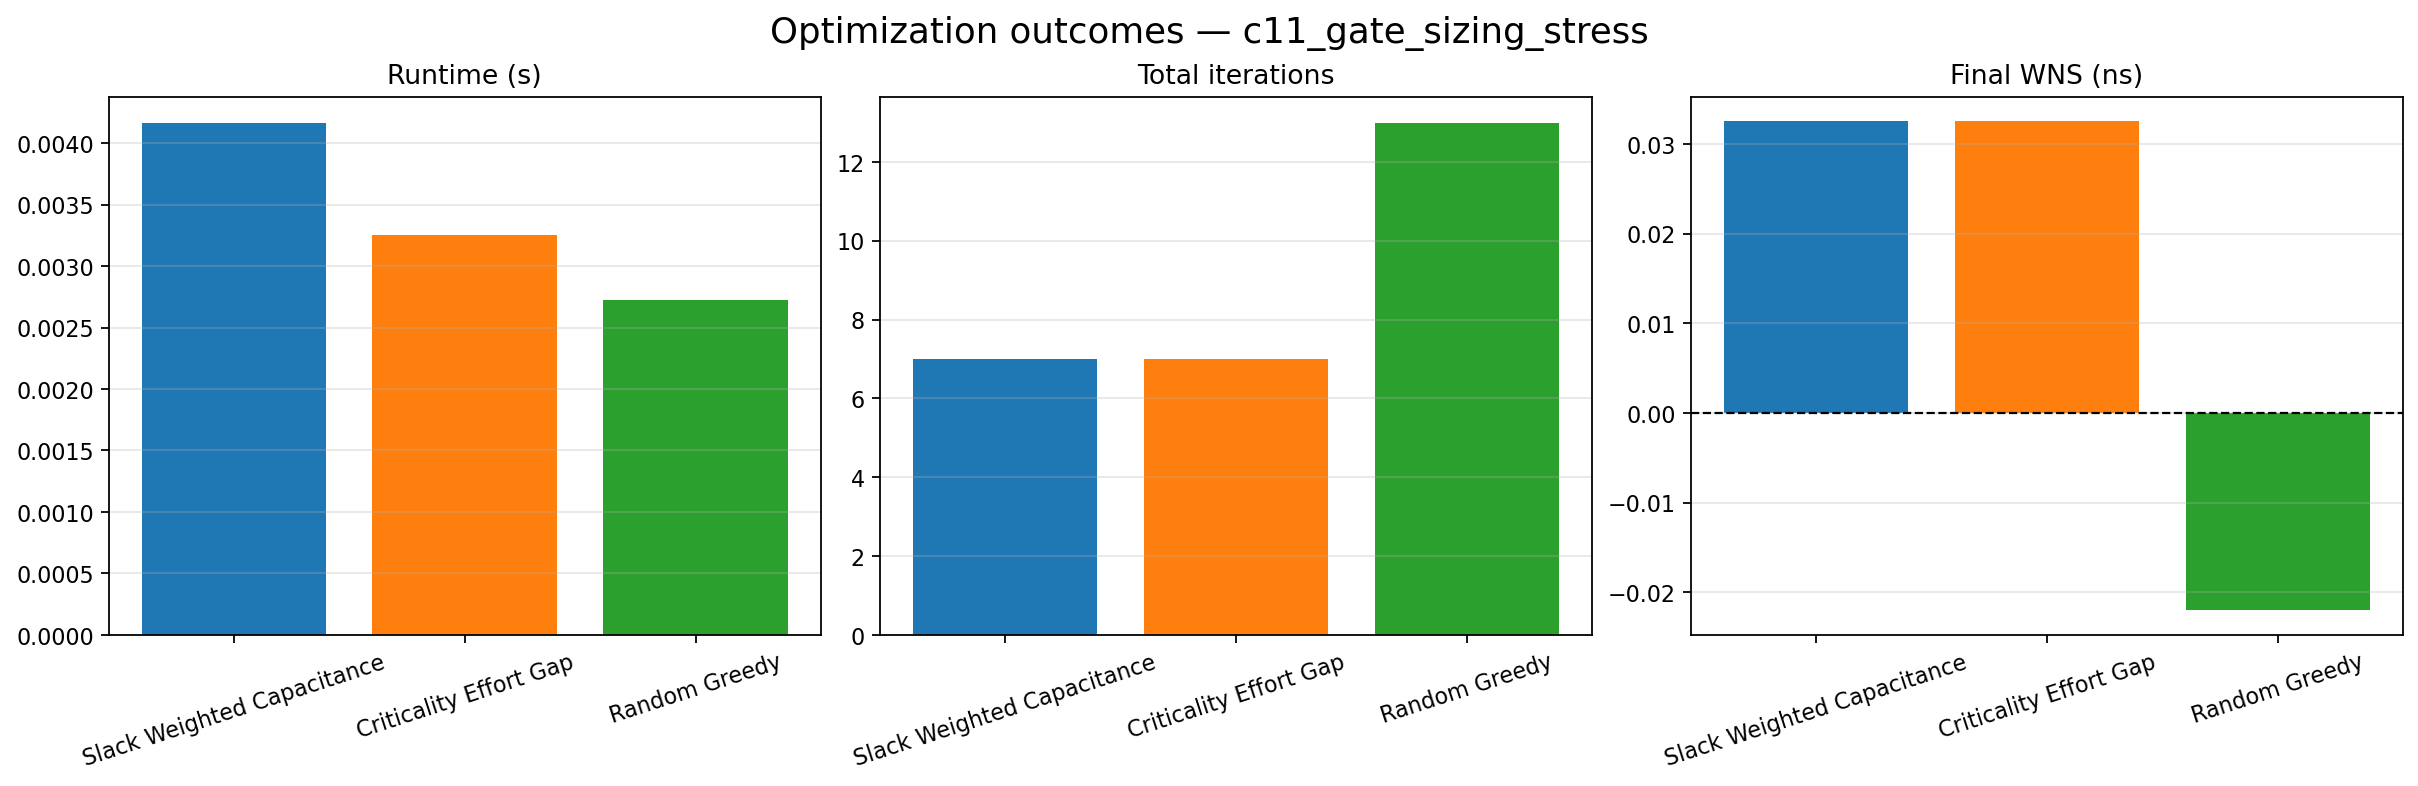
\includegraphics[width=\textwidth]{c11_gate_sizing_stress_outc.png}
    \caption{\texttt{c11\_gate\_sizing\_stress}: optimization outcomes summary.}
    \label{fig:app-c11-gate-sizing-stress-outc}
\end{figure}

\clearpage

\section{\texttt{c12\_monte\_carlo\_switching} (7 gates)}
\label{app:fig-c12-monte-carlo-switching}

\begin{figure}[H]
    \centering
    \begin{subfigure}[t]{0.48\textwidth}
        \centering
        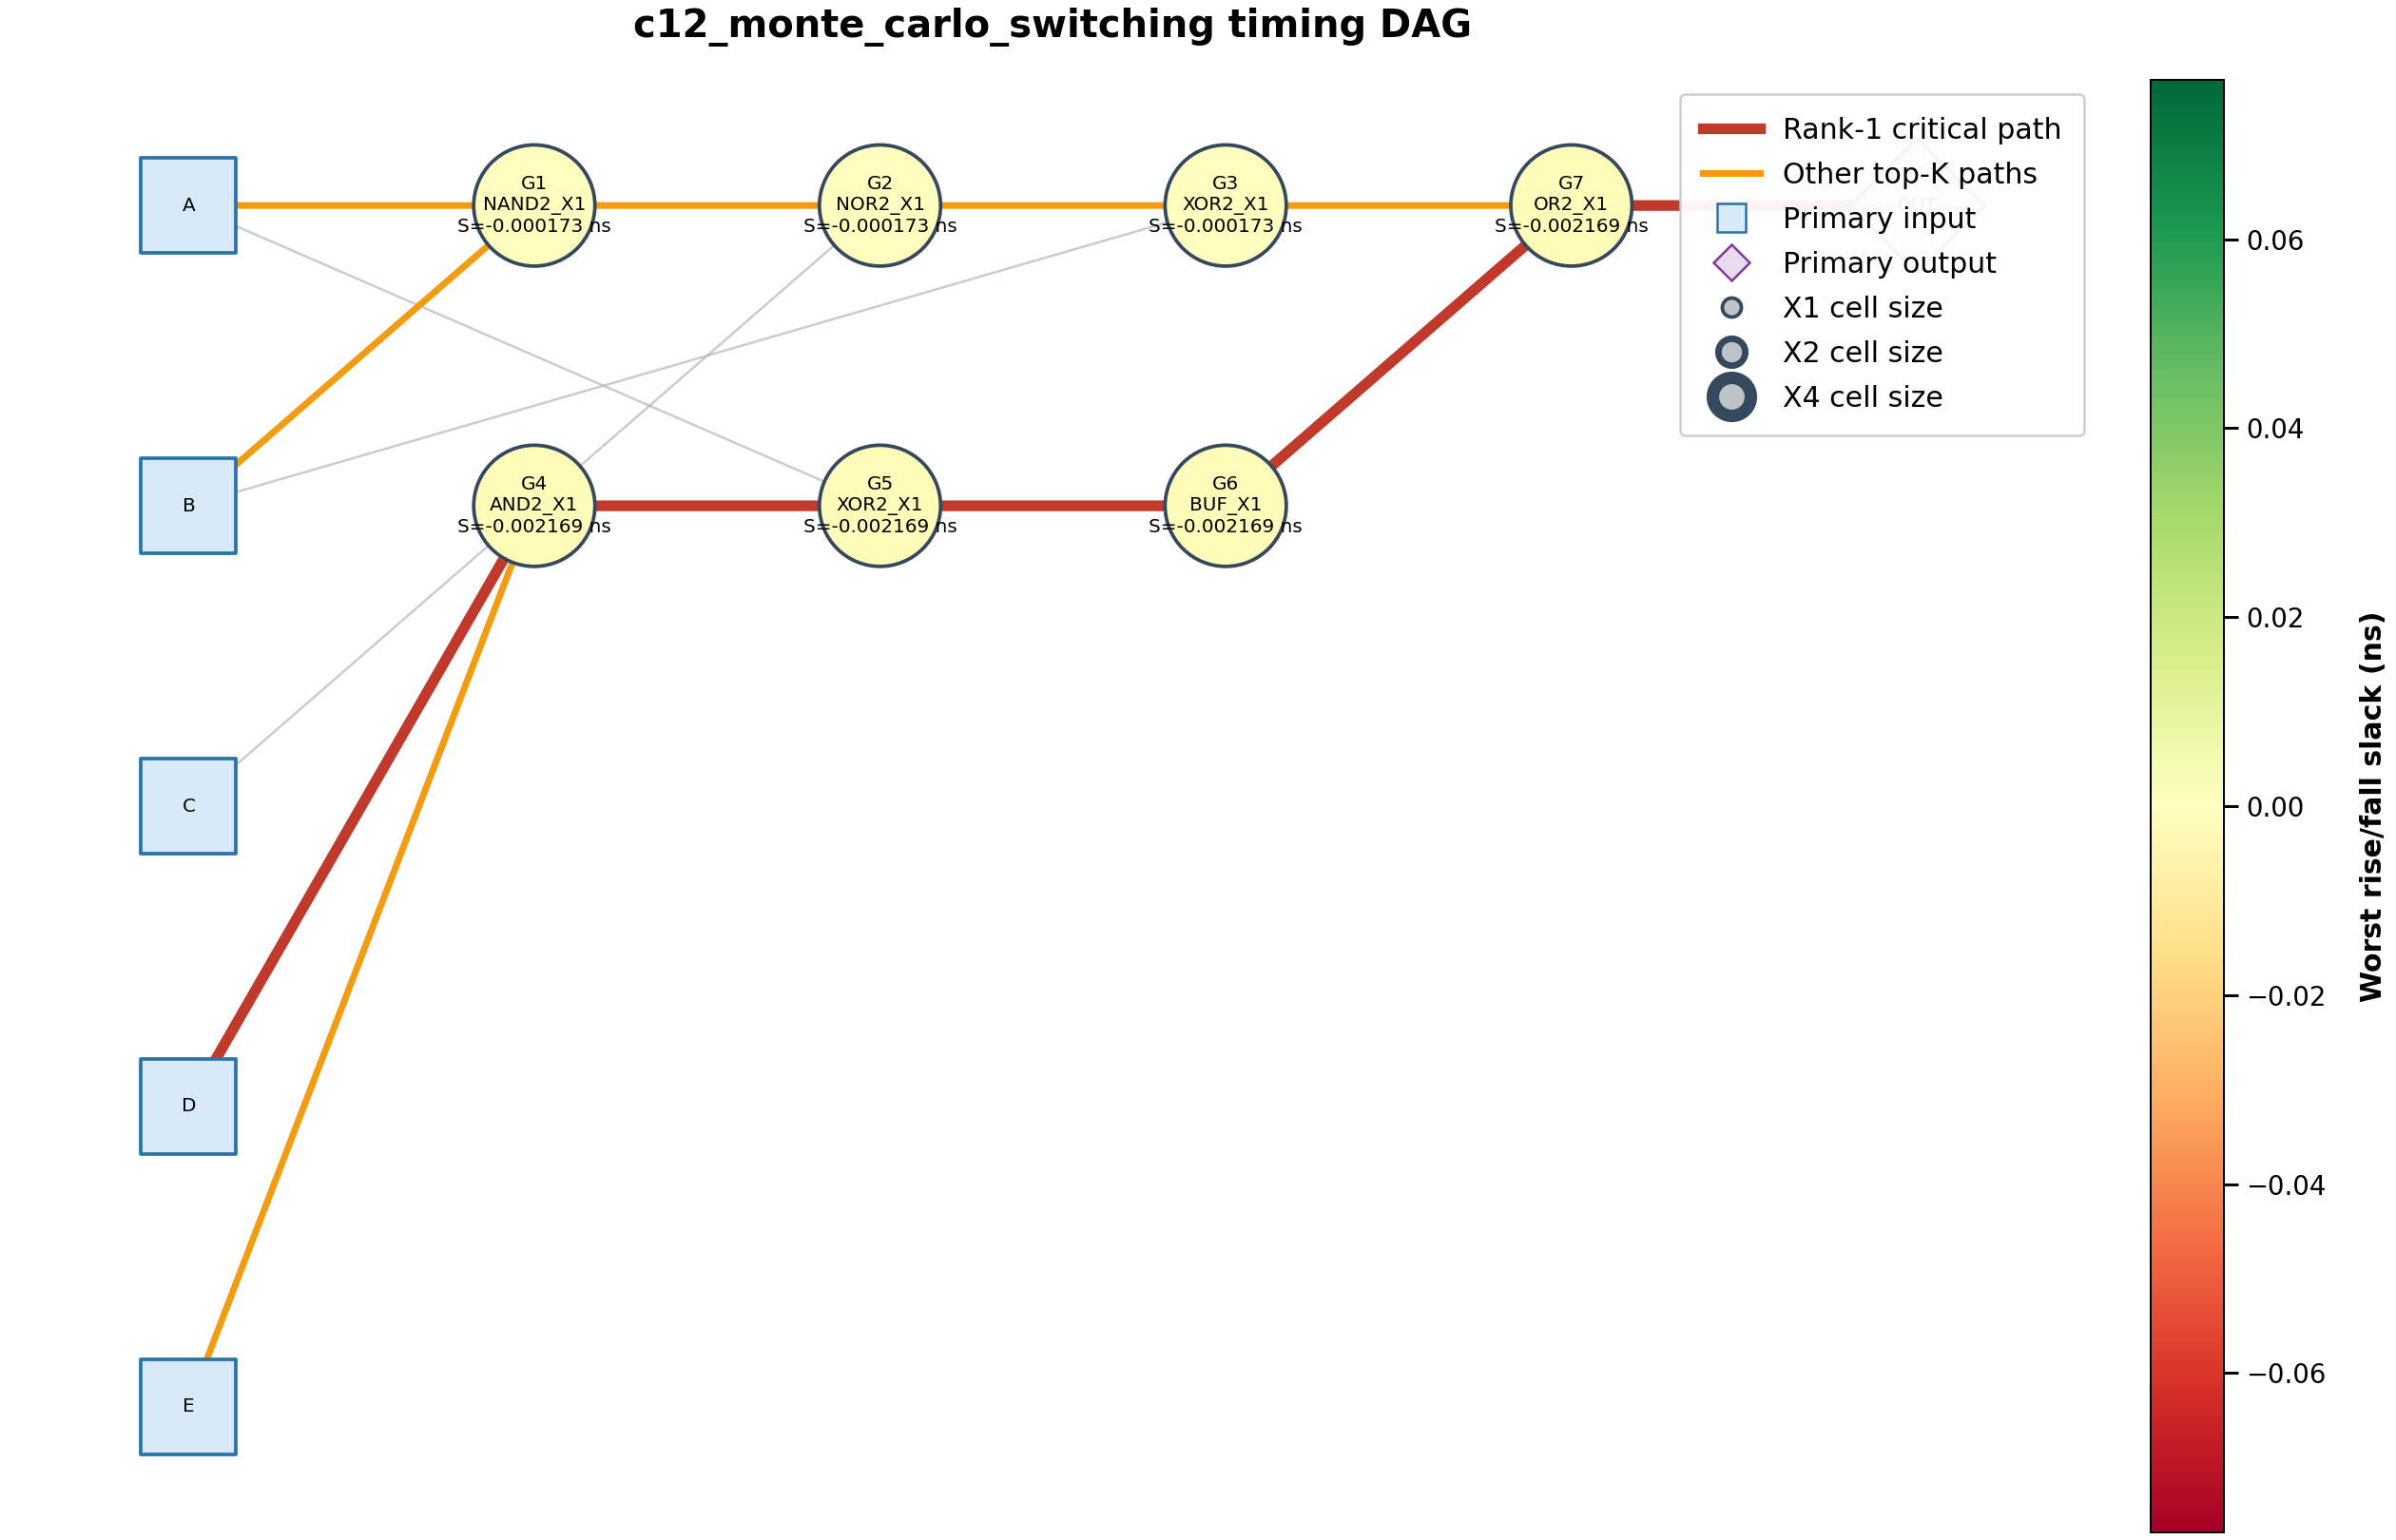
\includegraphics[width=\textwidth]{c12_monte_carlo_switching_pre.png}
        \caption{Pre-optimization}
    \end{subfigure}
    \hfill
    \begin{subfigure}[t]{0.48\textwidth}
        \centering
        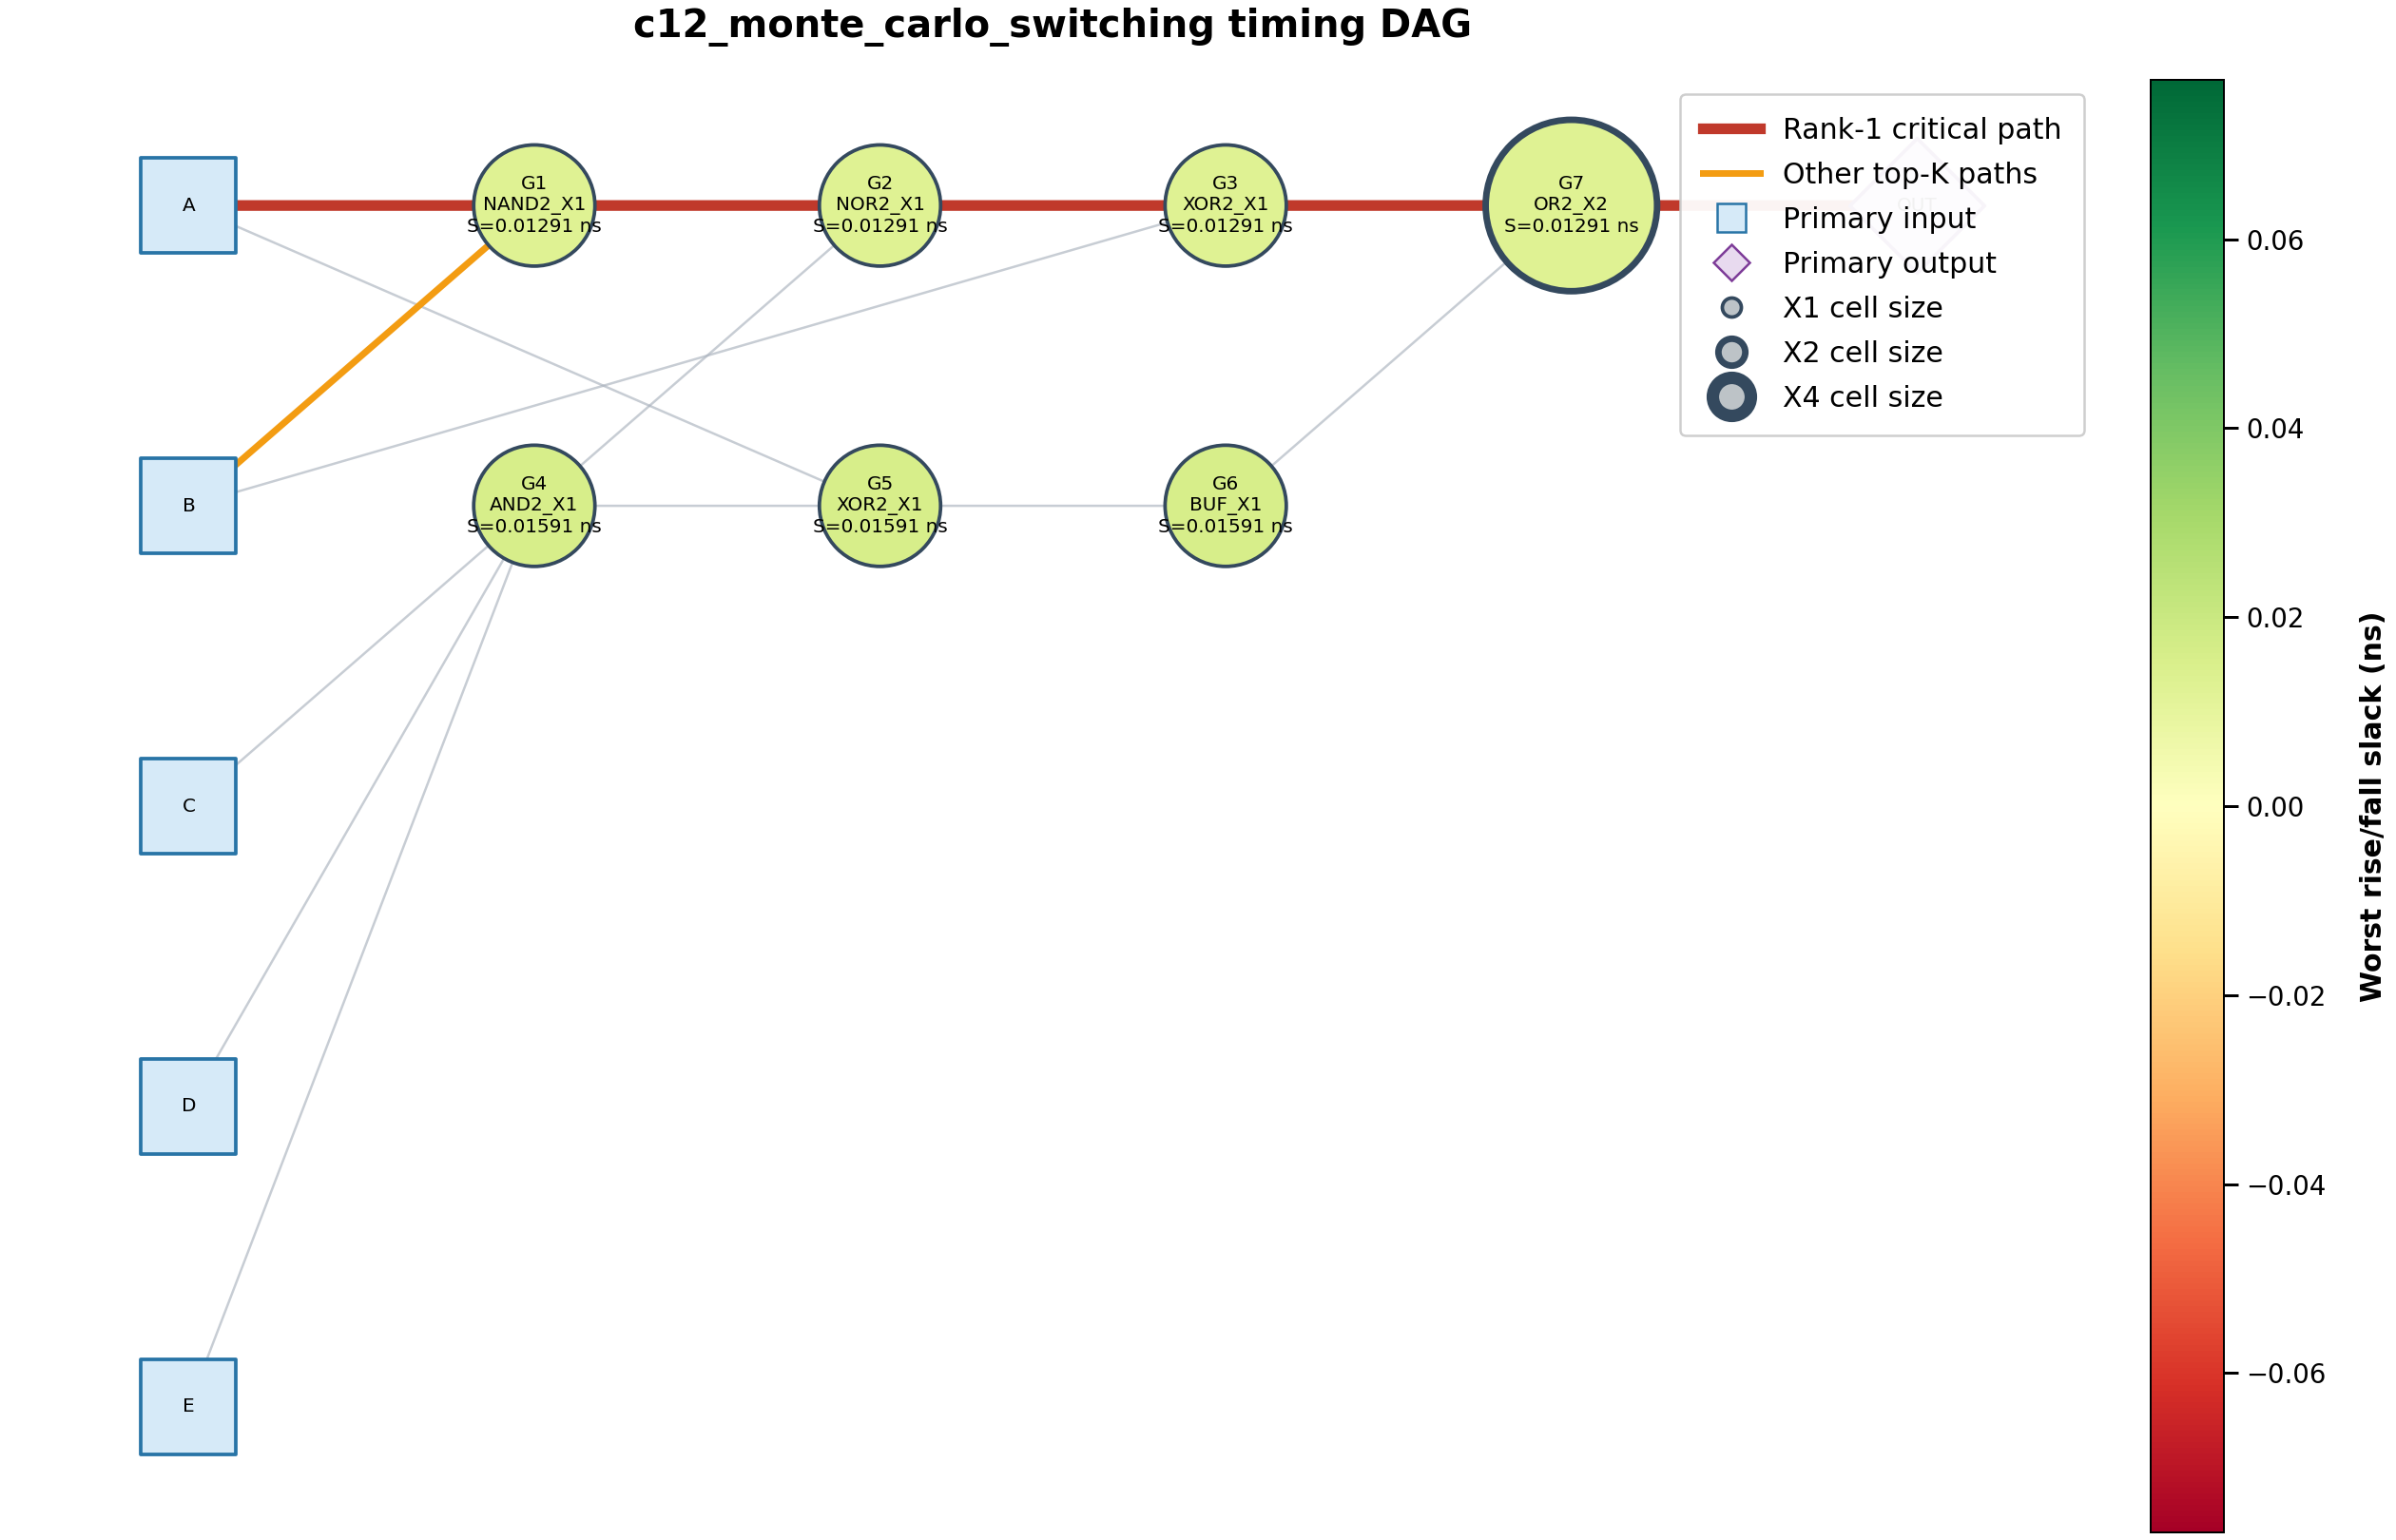
\includegraphics[width=\textwidth]{c12_monte_carlo_switching_post.png}
        \caption{Post-optimization}
    \end{subfigure}
    \caption{\texttt{c12\_monte\_carlo\_switching}: circuit diagrams, nodes colored by slack,
    critical path highlighted.}
    \label{fig:app-c12-monte-carlo-switching-graphs}
\end{figure}

\begin{figure}[H]
    \centering
    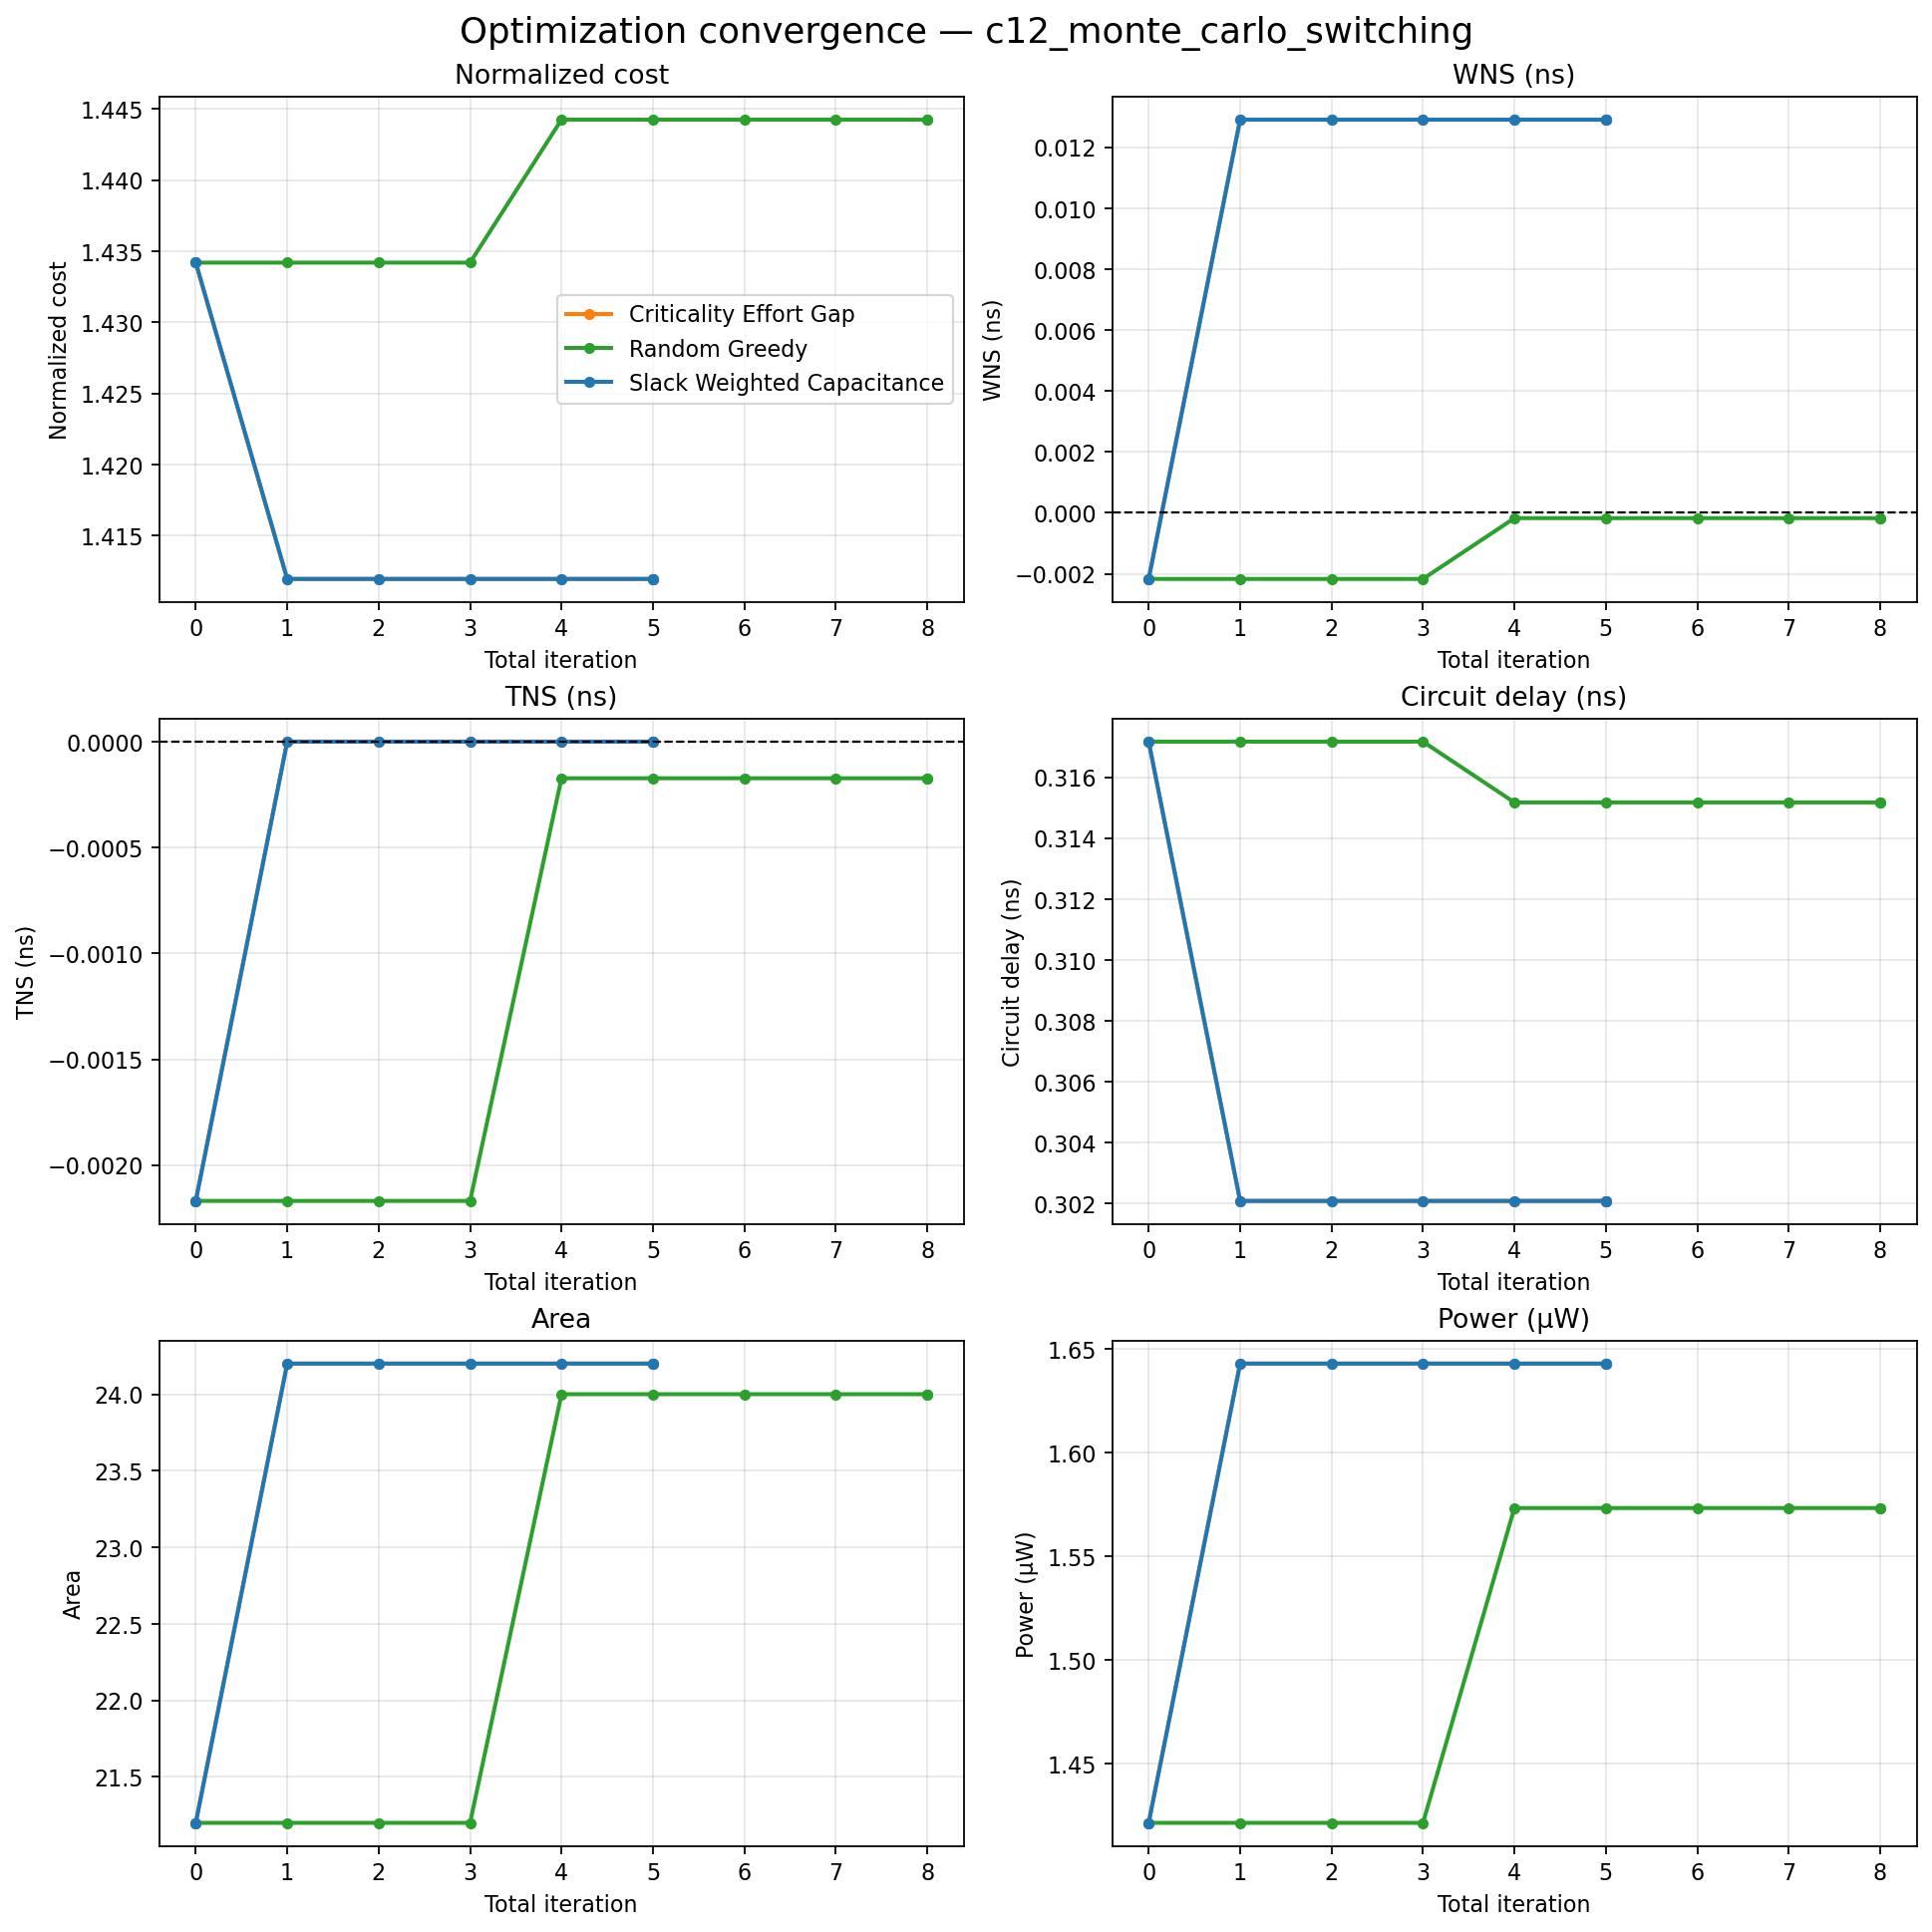
\includegraphics[width=\textwidth]{c12_monte_carlo_switching_conv.png}
    \caption{\texttt{c12\_monte\_carlo\_switching}: optimization convergence trace.}
    \label{fig:app-c12-monte-carlo-switching-conv}
\end{figure}

\begin{figure}[H]
    \centering
    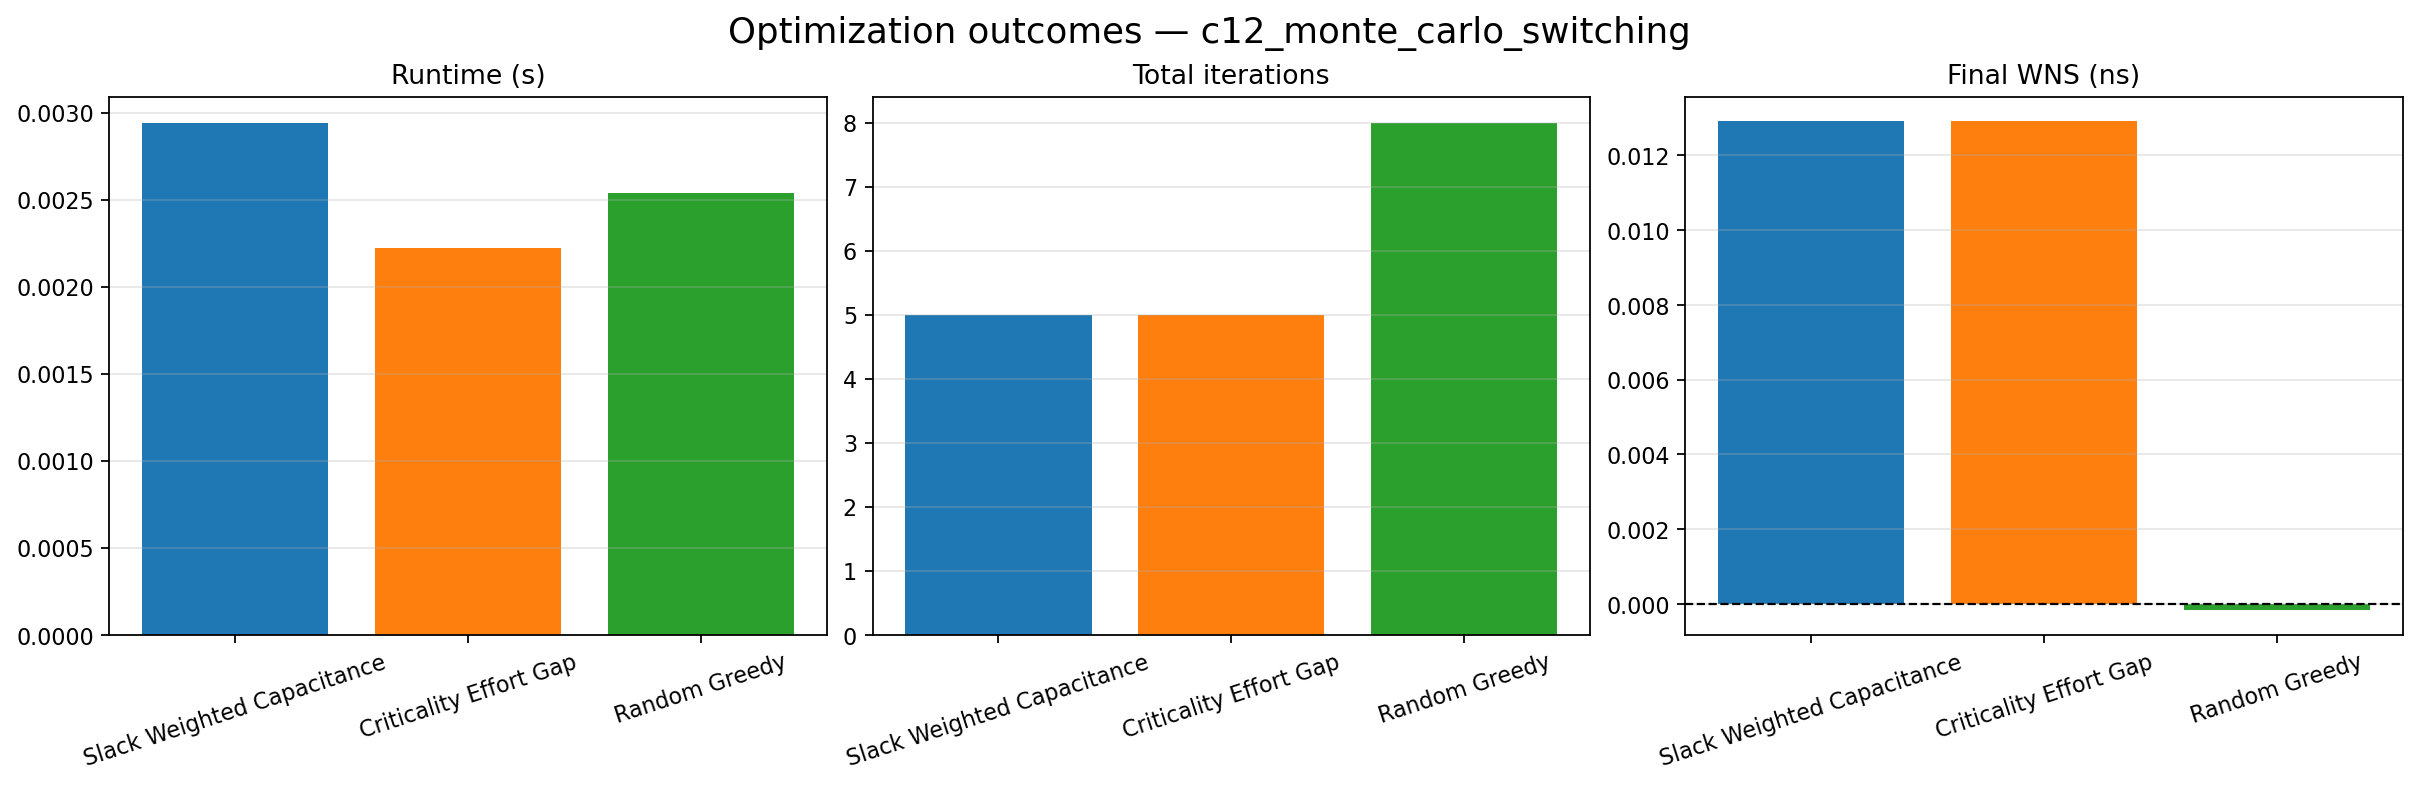
\includegraphics[width=\textwidth]{c12_monte_carlo_switching_outc.png}
    \caption{\texttt{c12\_monte\_carlo\_switching}: optimization outcomes summary.}
    \label{fig:app-c12-monte-carlo-switching-outc}
\end{figure}

\clearpage

\section{\texttt{c13\_large\_reconvergent\_network} (74 gates)}
\label{app:fig-c13-large-reconvergent-network}

\begin{figure}[H]
    \centering
    \begin{subfigure}[t]{0.48\textwidth}
        \centering
        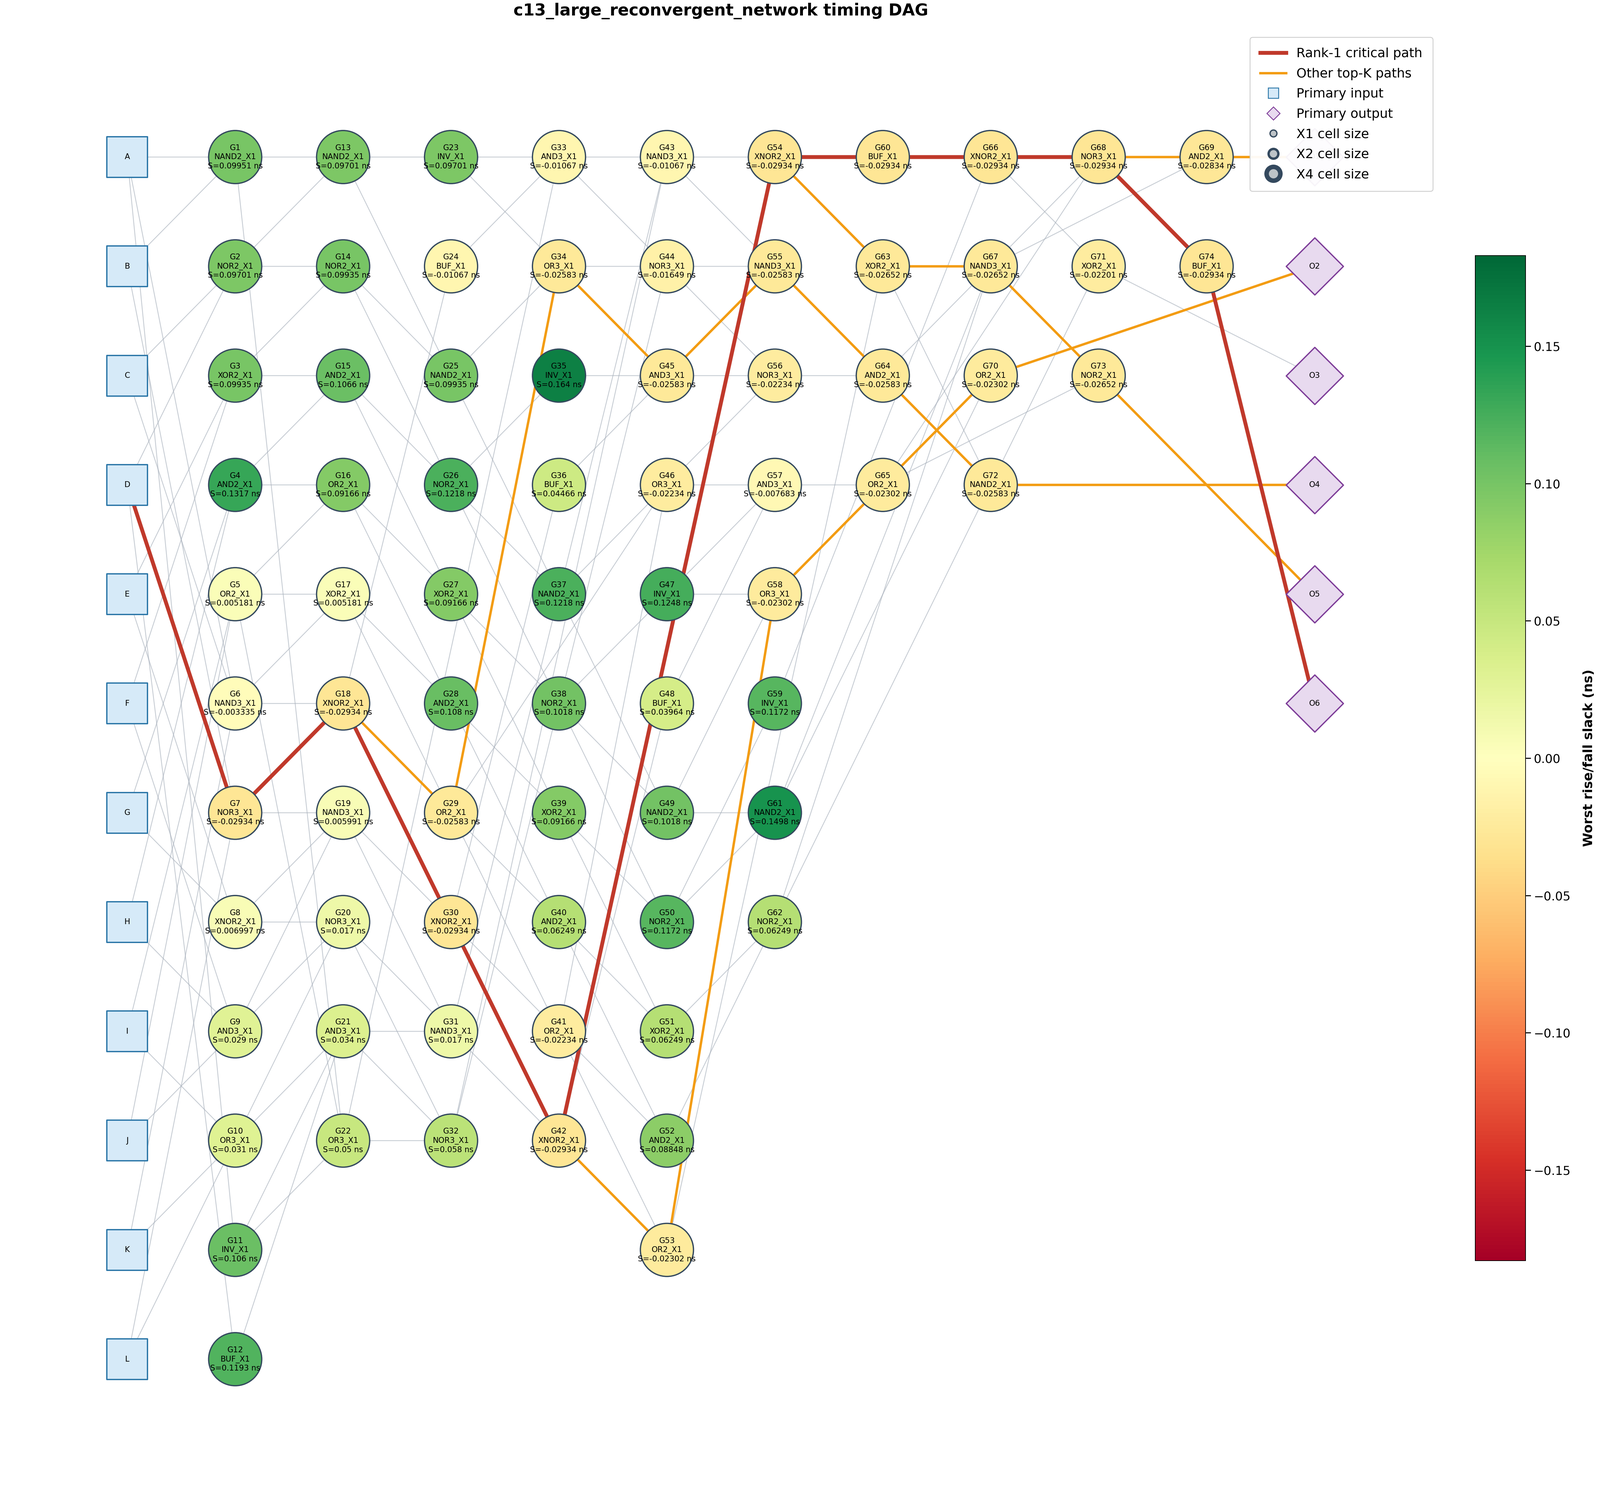
\includegraphics[width=\textwidth]{c13_large_reconvergent_network_pre.png}
        \caption{Pre-optimization}
    \end{subfigure}
    \hfill
    \begin{subfigure}[t]{0.48\textwidth}
        \centering
        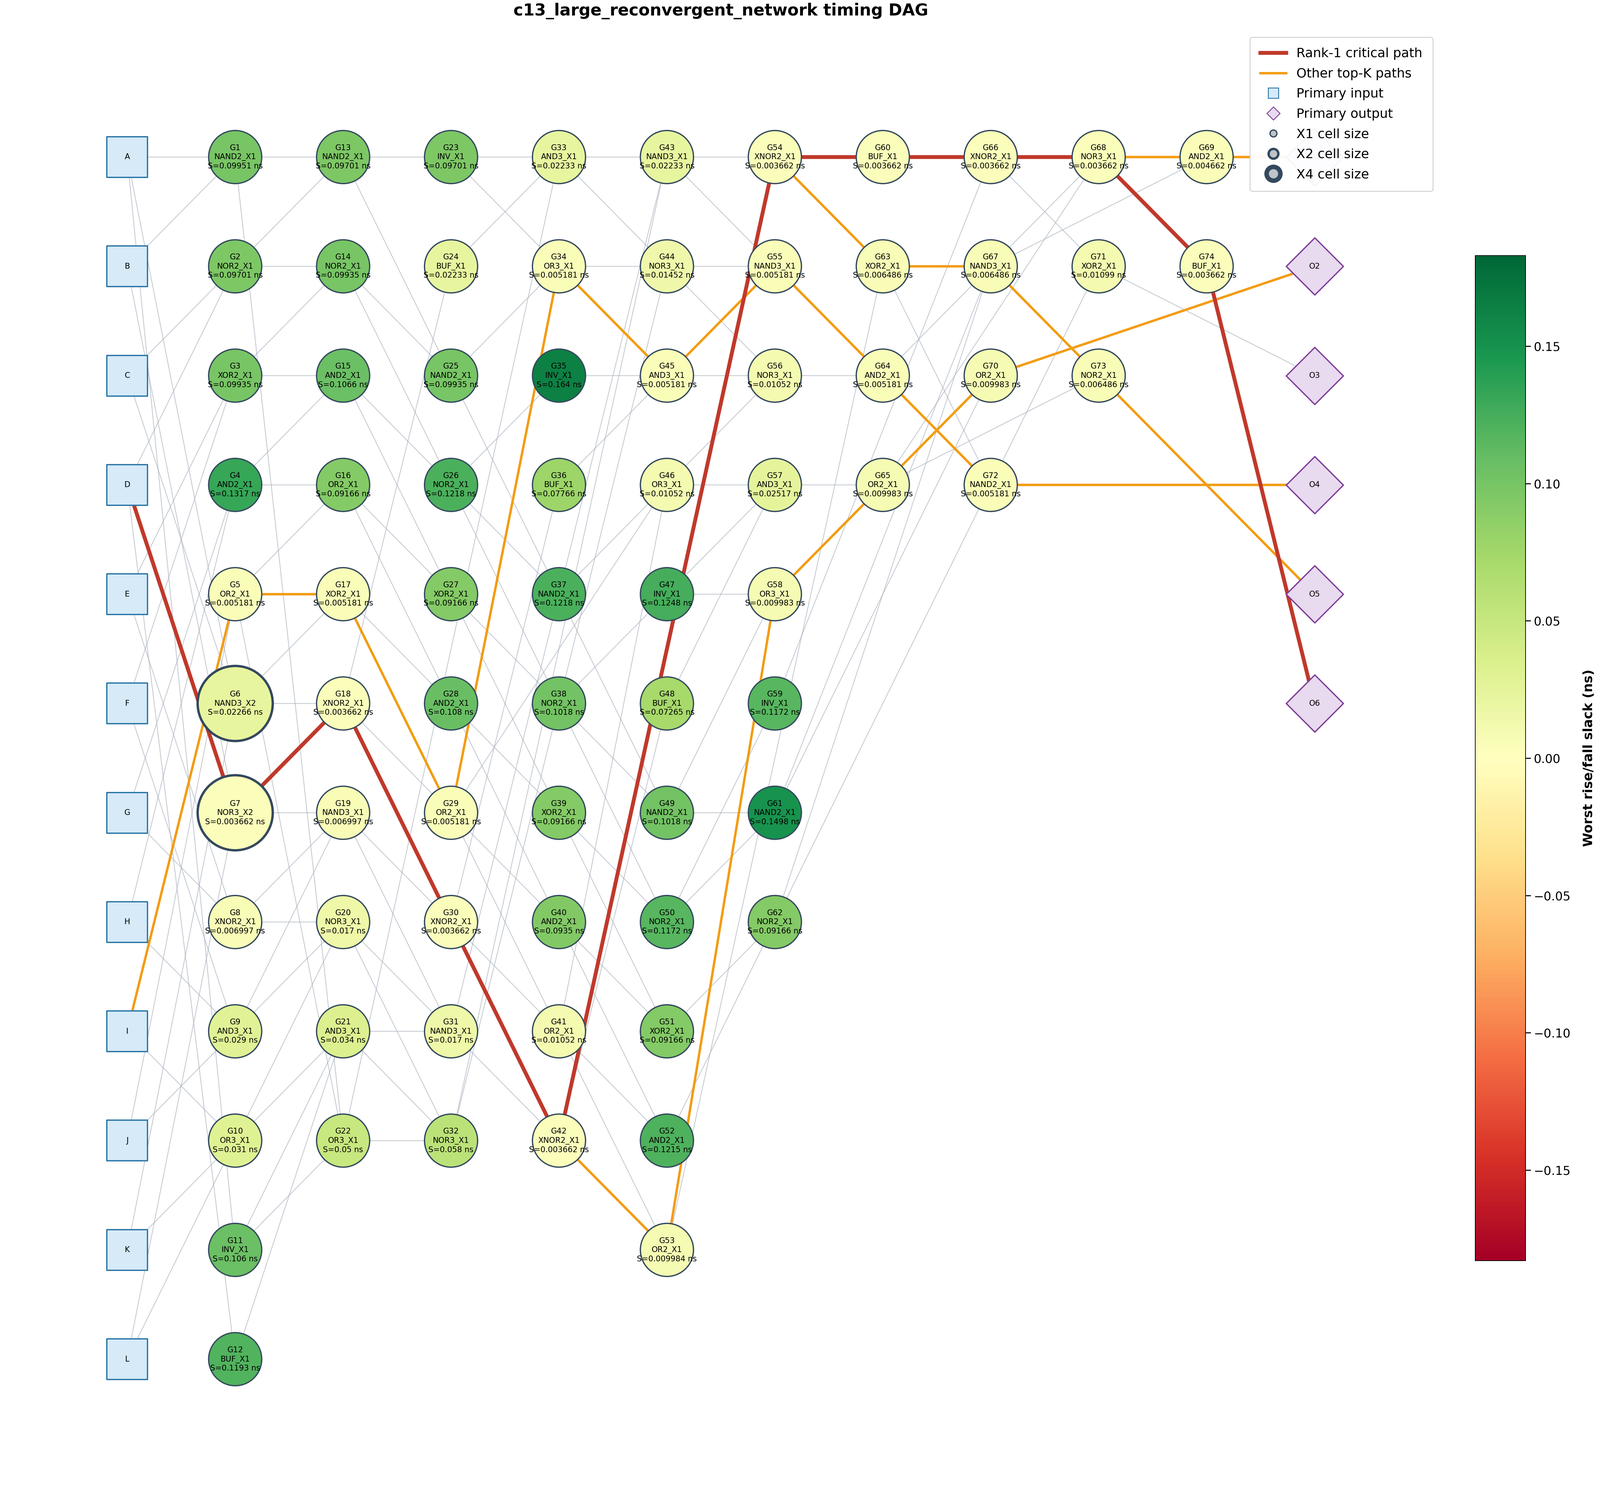
\includegraphics[width=\textwidth]{c13_large_reconvergent_network_post.png}
        \caption{Post-optimization}
    \end{subfigure}
    \caption{\texttt{c13\_large\_reconvergent\_network}: circuit diagrams, nodes colored by slack,
    critical path highlighted.}
    \label{fig:app-c13-large-reconvergent-network-graphs}
\end{figure}

\begin{figure}[H]
    \centering
    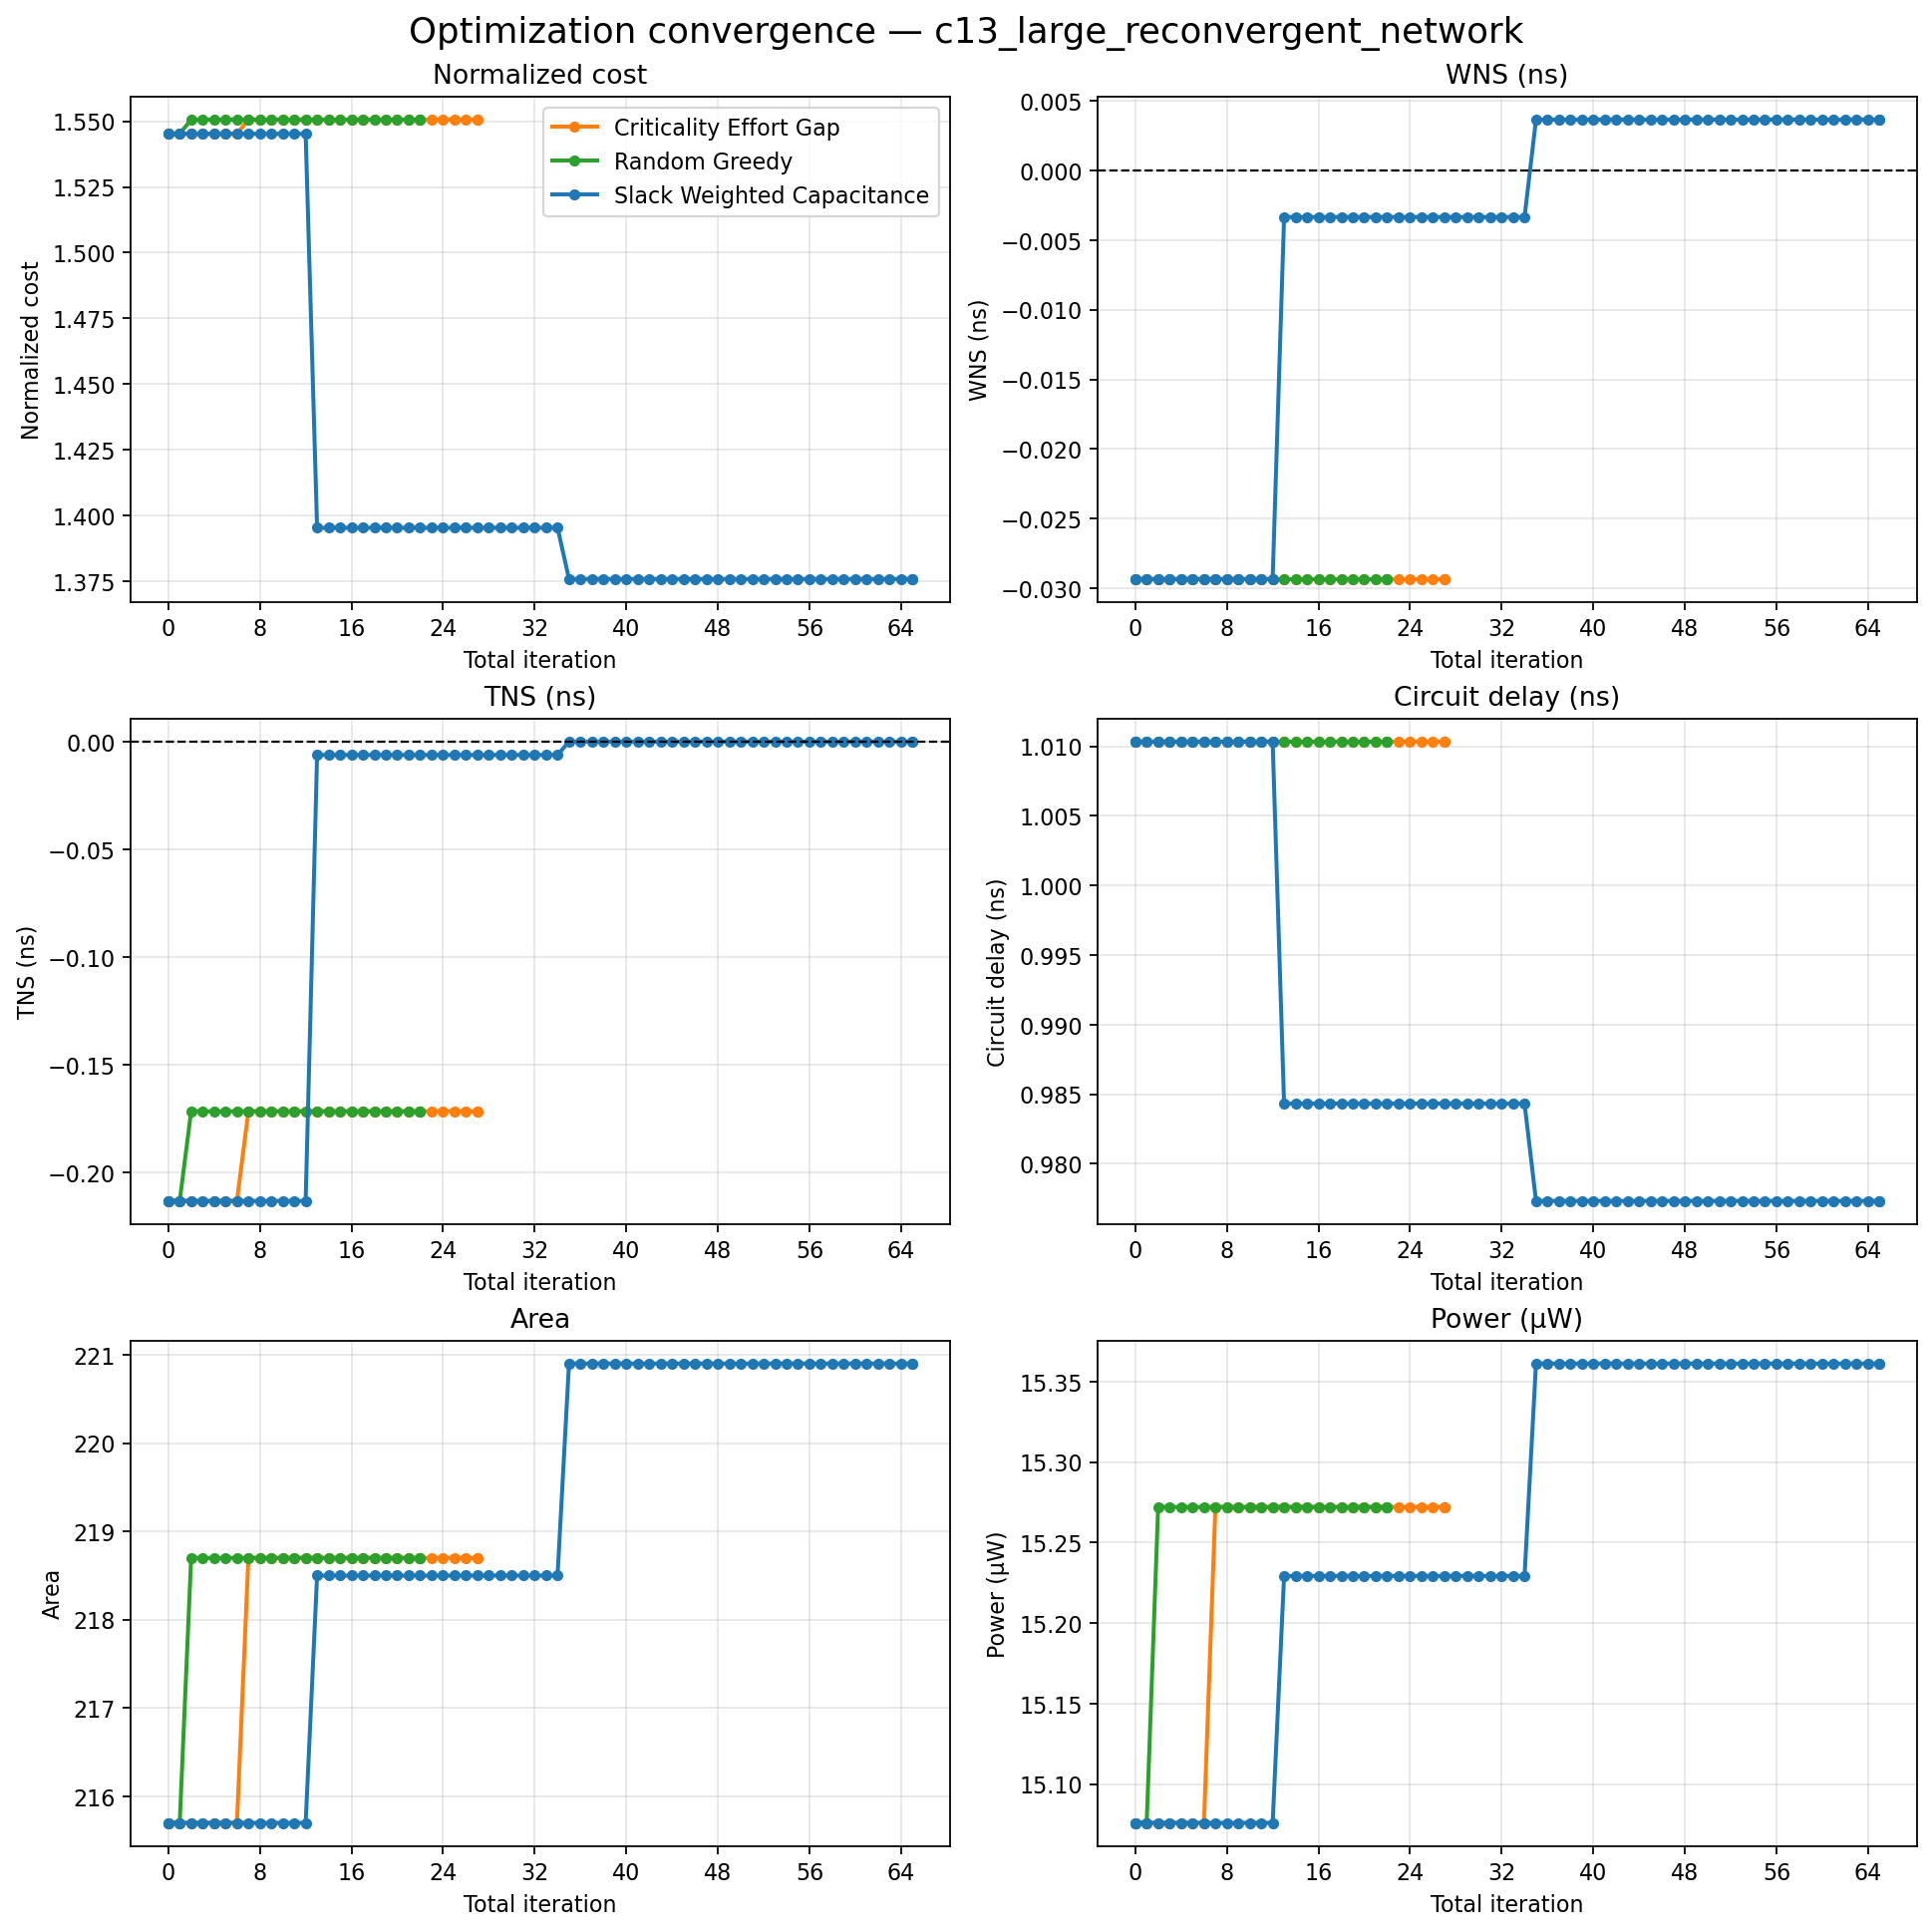
\includegraphics[width=\textwidth]{c13_large_reconvergent_network_conv.png}
    \caption{\texttt{c13\_large\_reconvergent\_network}: optimization convergence trace.}
    \label{fig:app-c13-large-reconvergent-network-conv}
\end{figure}

\begin{figure}[H]
    \centering
    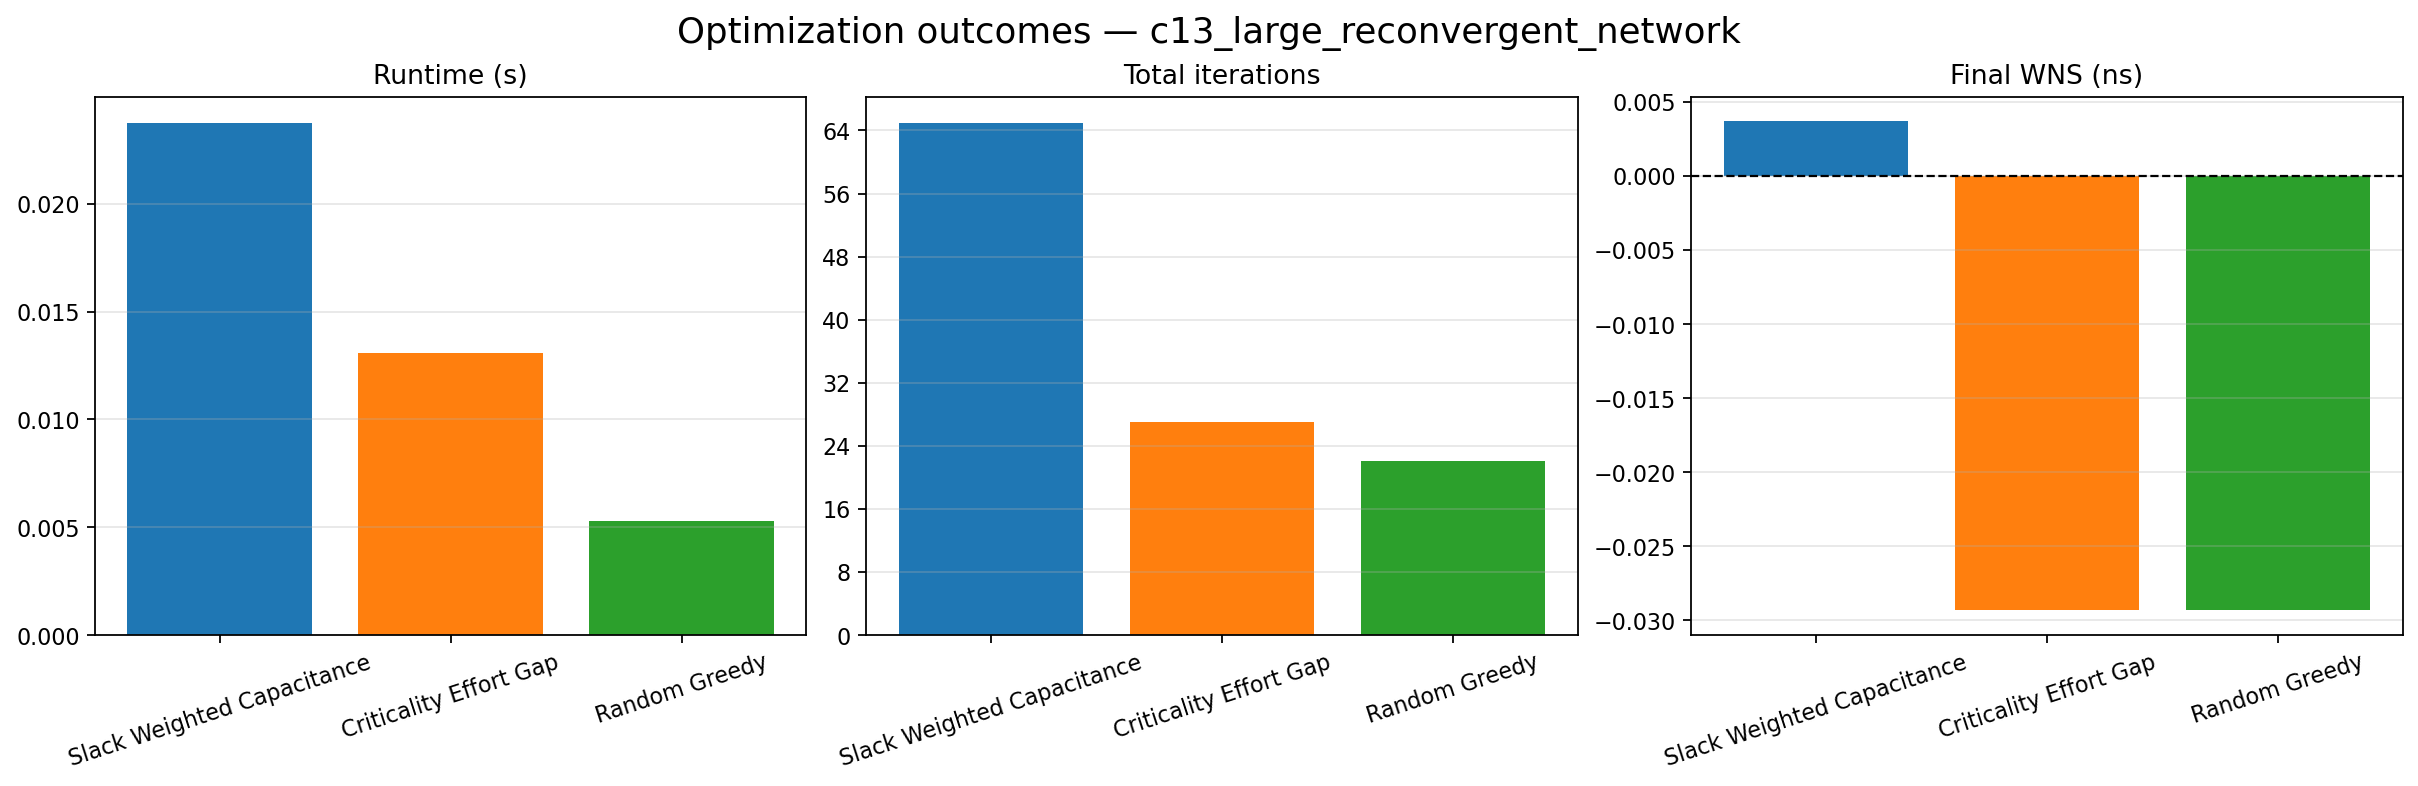
\includegraphics[width=\textwidth]{c13_large_reconvergent_network_outc.png}
    \caption{\texttt{c13\_large\_reconvergent\_network}: optimization outcomes summary.}
    \label{fig:app-c13-large-reconvergent-network-outc}
\end{figure}

\clearpage

\section{\texttt{c14\_layered\_reconvergent\_fabric} (104 gates)}
\label{app:fig-c14-layered-reconvergent-fabric}

\begin{figure}[H]
    \centering
    \begin{subfigure}[t]{0.48\textwidth}
        \centering
        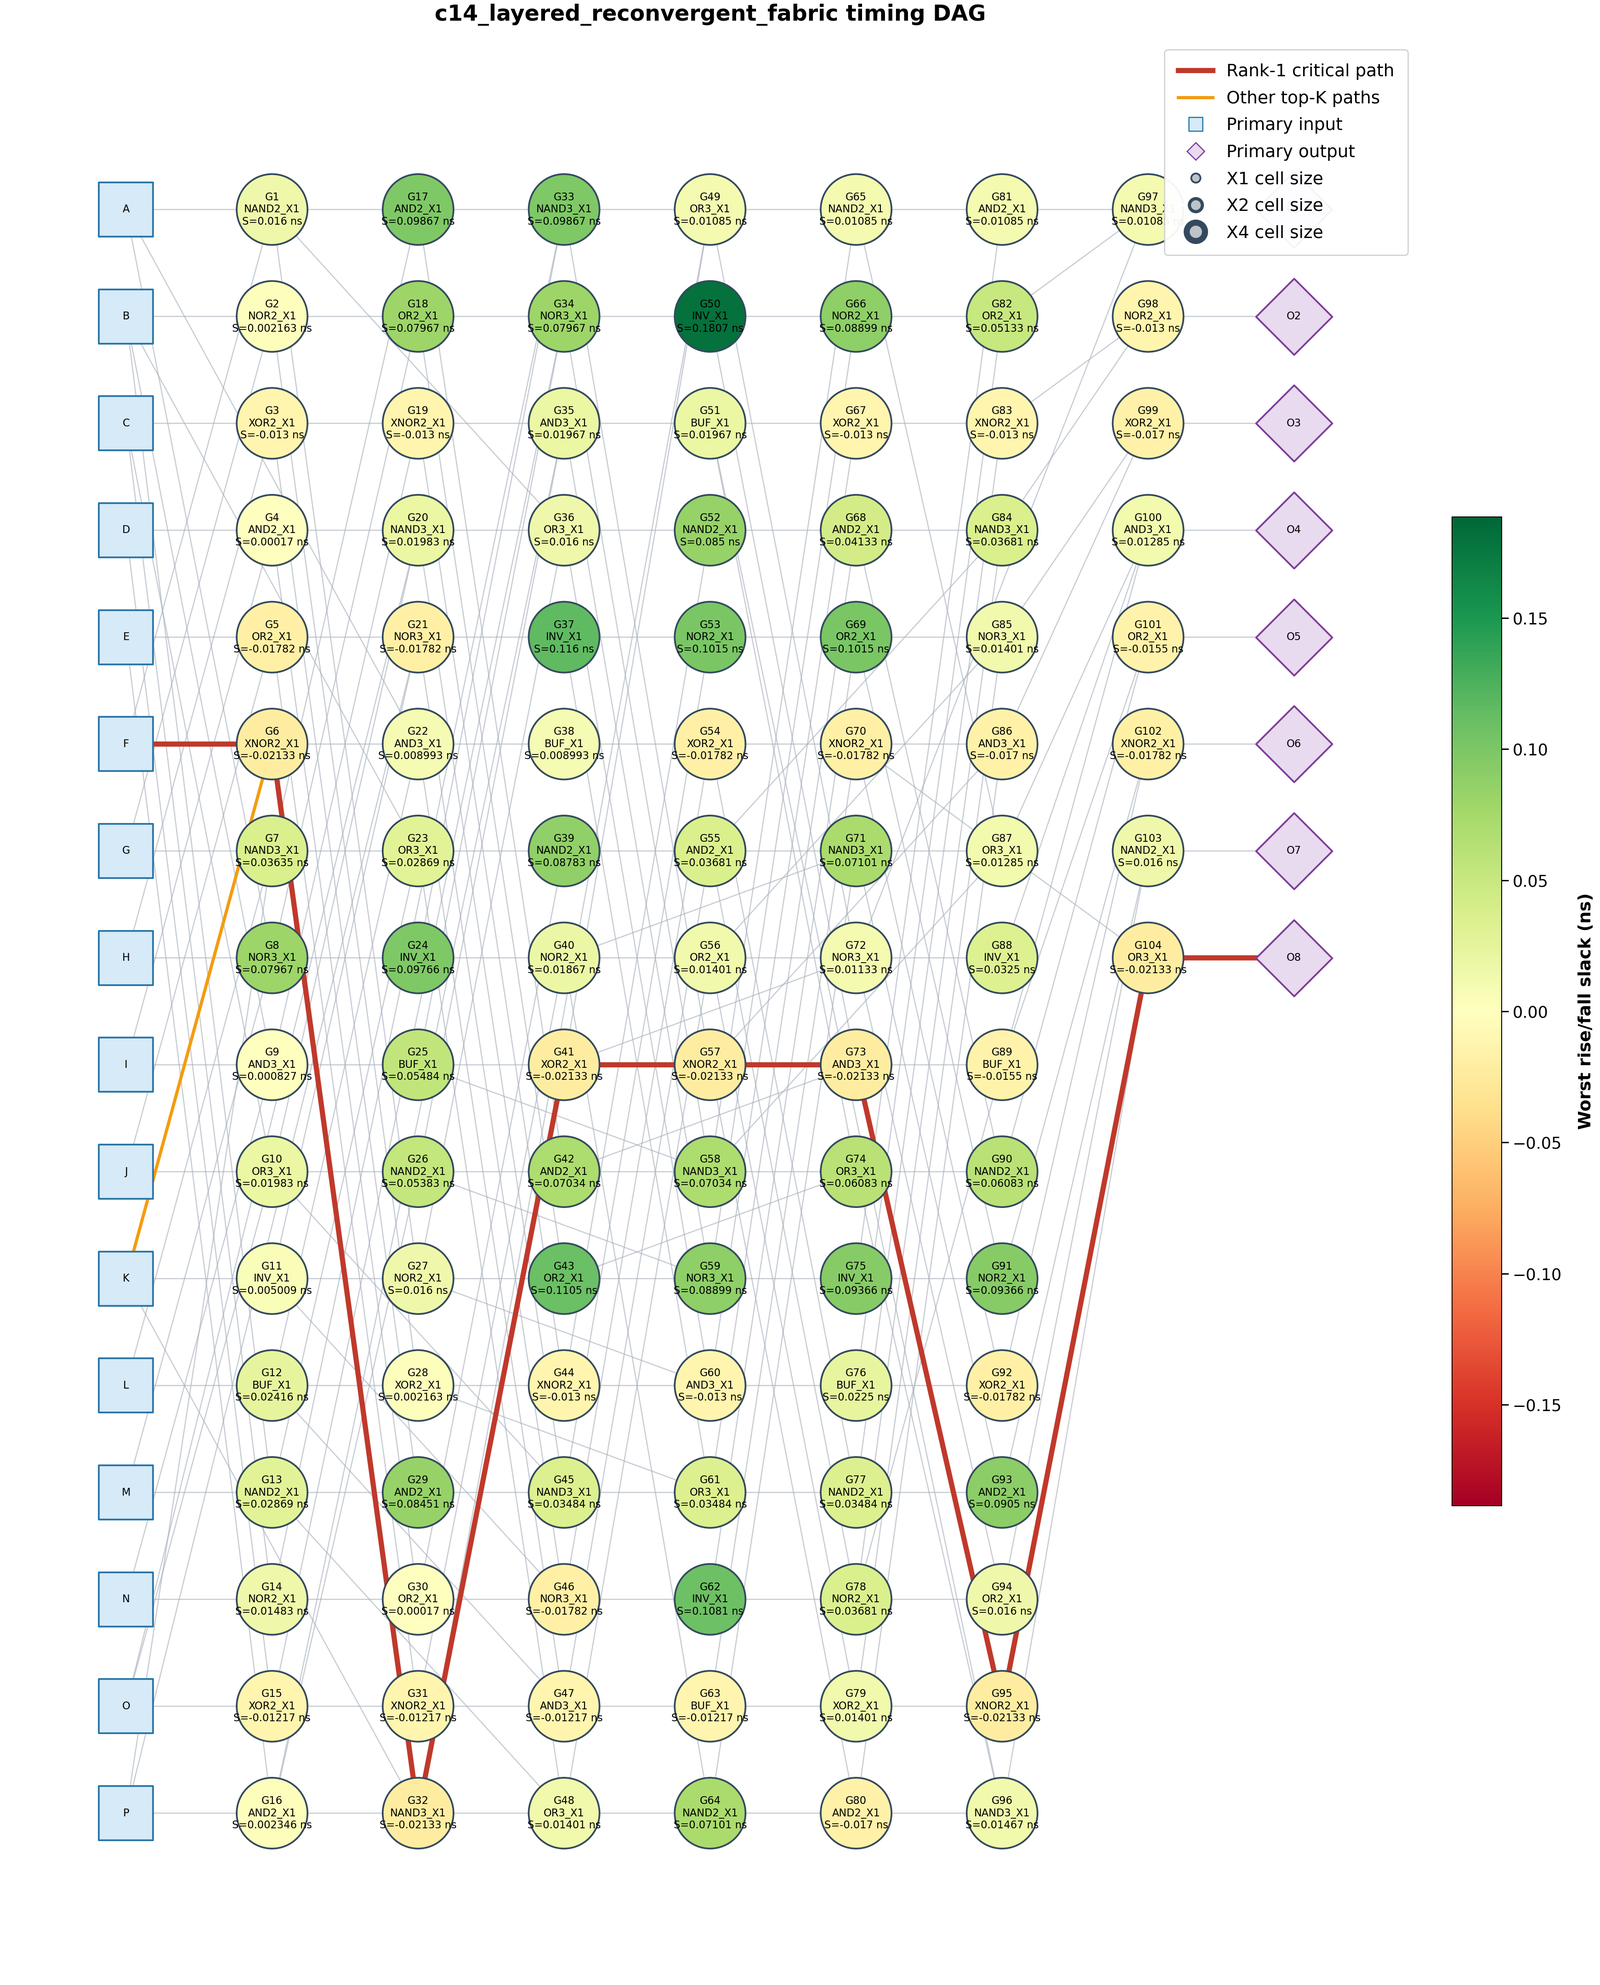
\includegraphics[width=\textwidth]{c14_layered_reconvergent_fabric_pre.png}
        \caption{Pre-optimization}
    \end{subfigure}
    \hfill
    \begin{subfigure}[t]{0.48\textwidth}
        \centering
        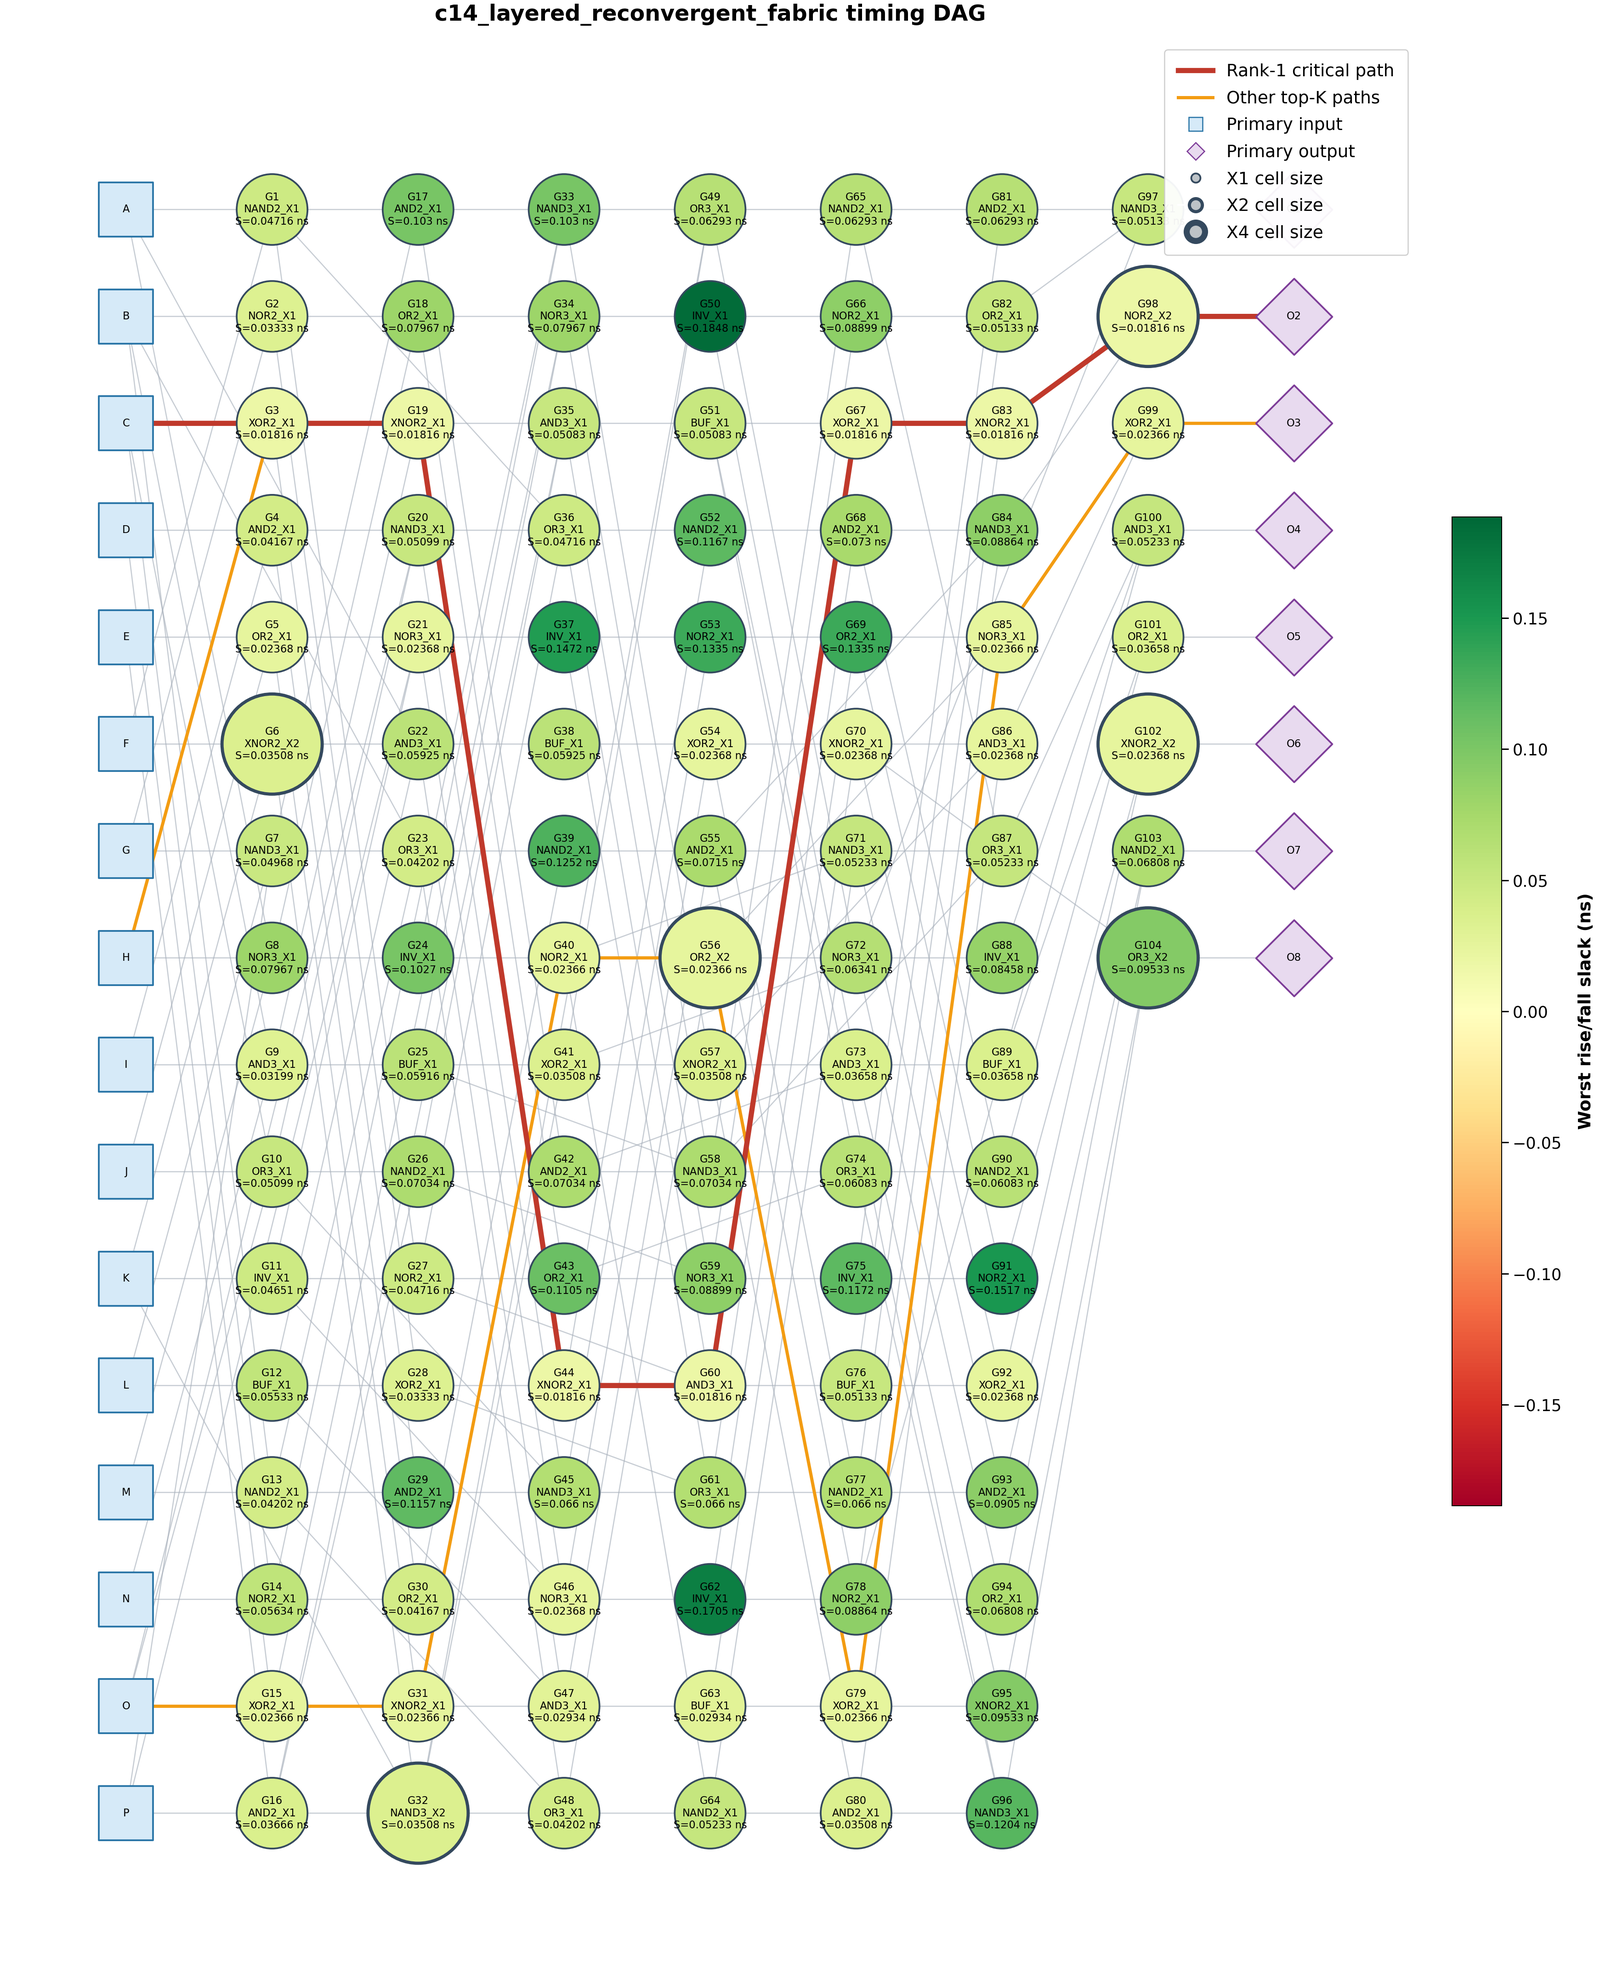
\includegraphics[width=\textwidth]{c14_layered_reconvergent_fabric_post.png}
        \caption{Post-optimization}
    \end{subfigure}
    \caption{\texttt{c14\_layered\_reconvergent\_fabric}: circuit diagrams, nodes colored by slack,
    critical path highlighted.}
    \label{fig:app-c14-layered-reconvergent-fabric-graphs}
\end{figure}

\begin{figure}[H]
    \centering
    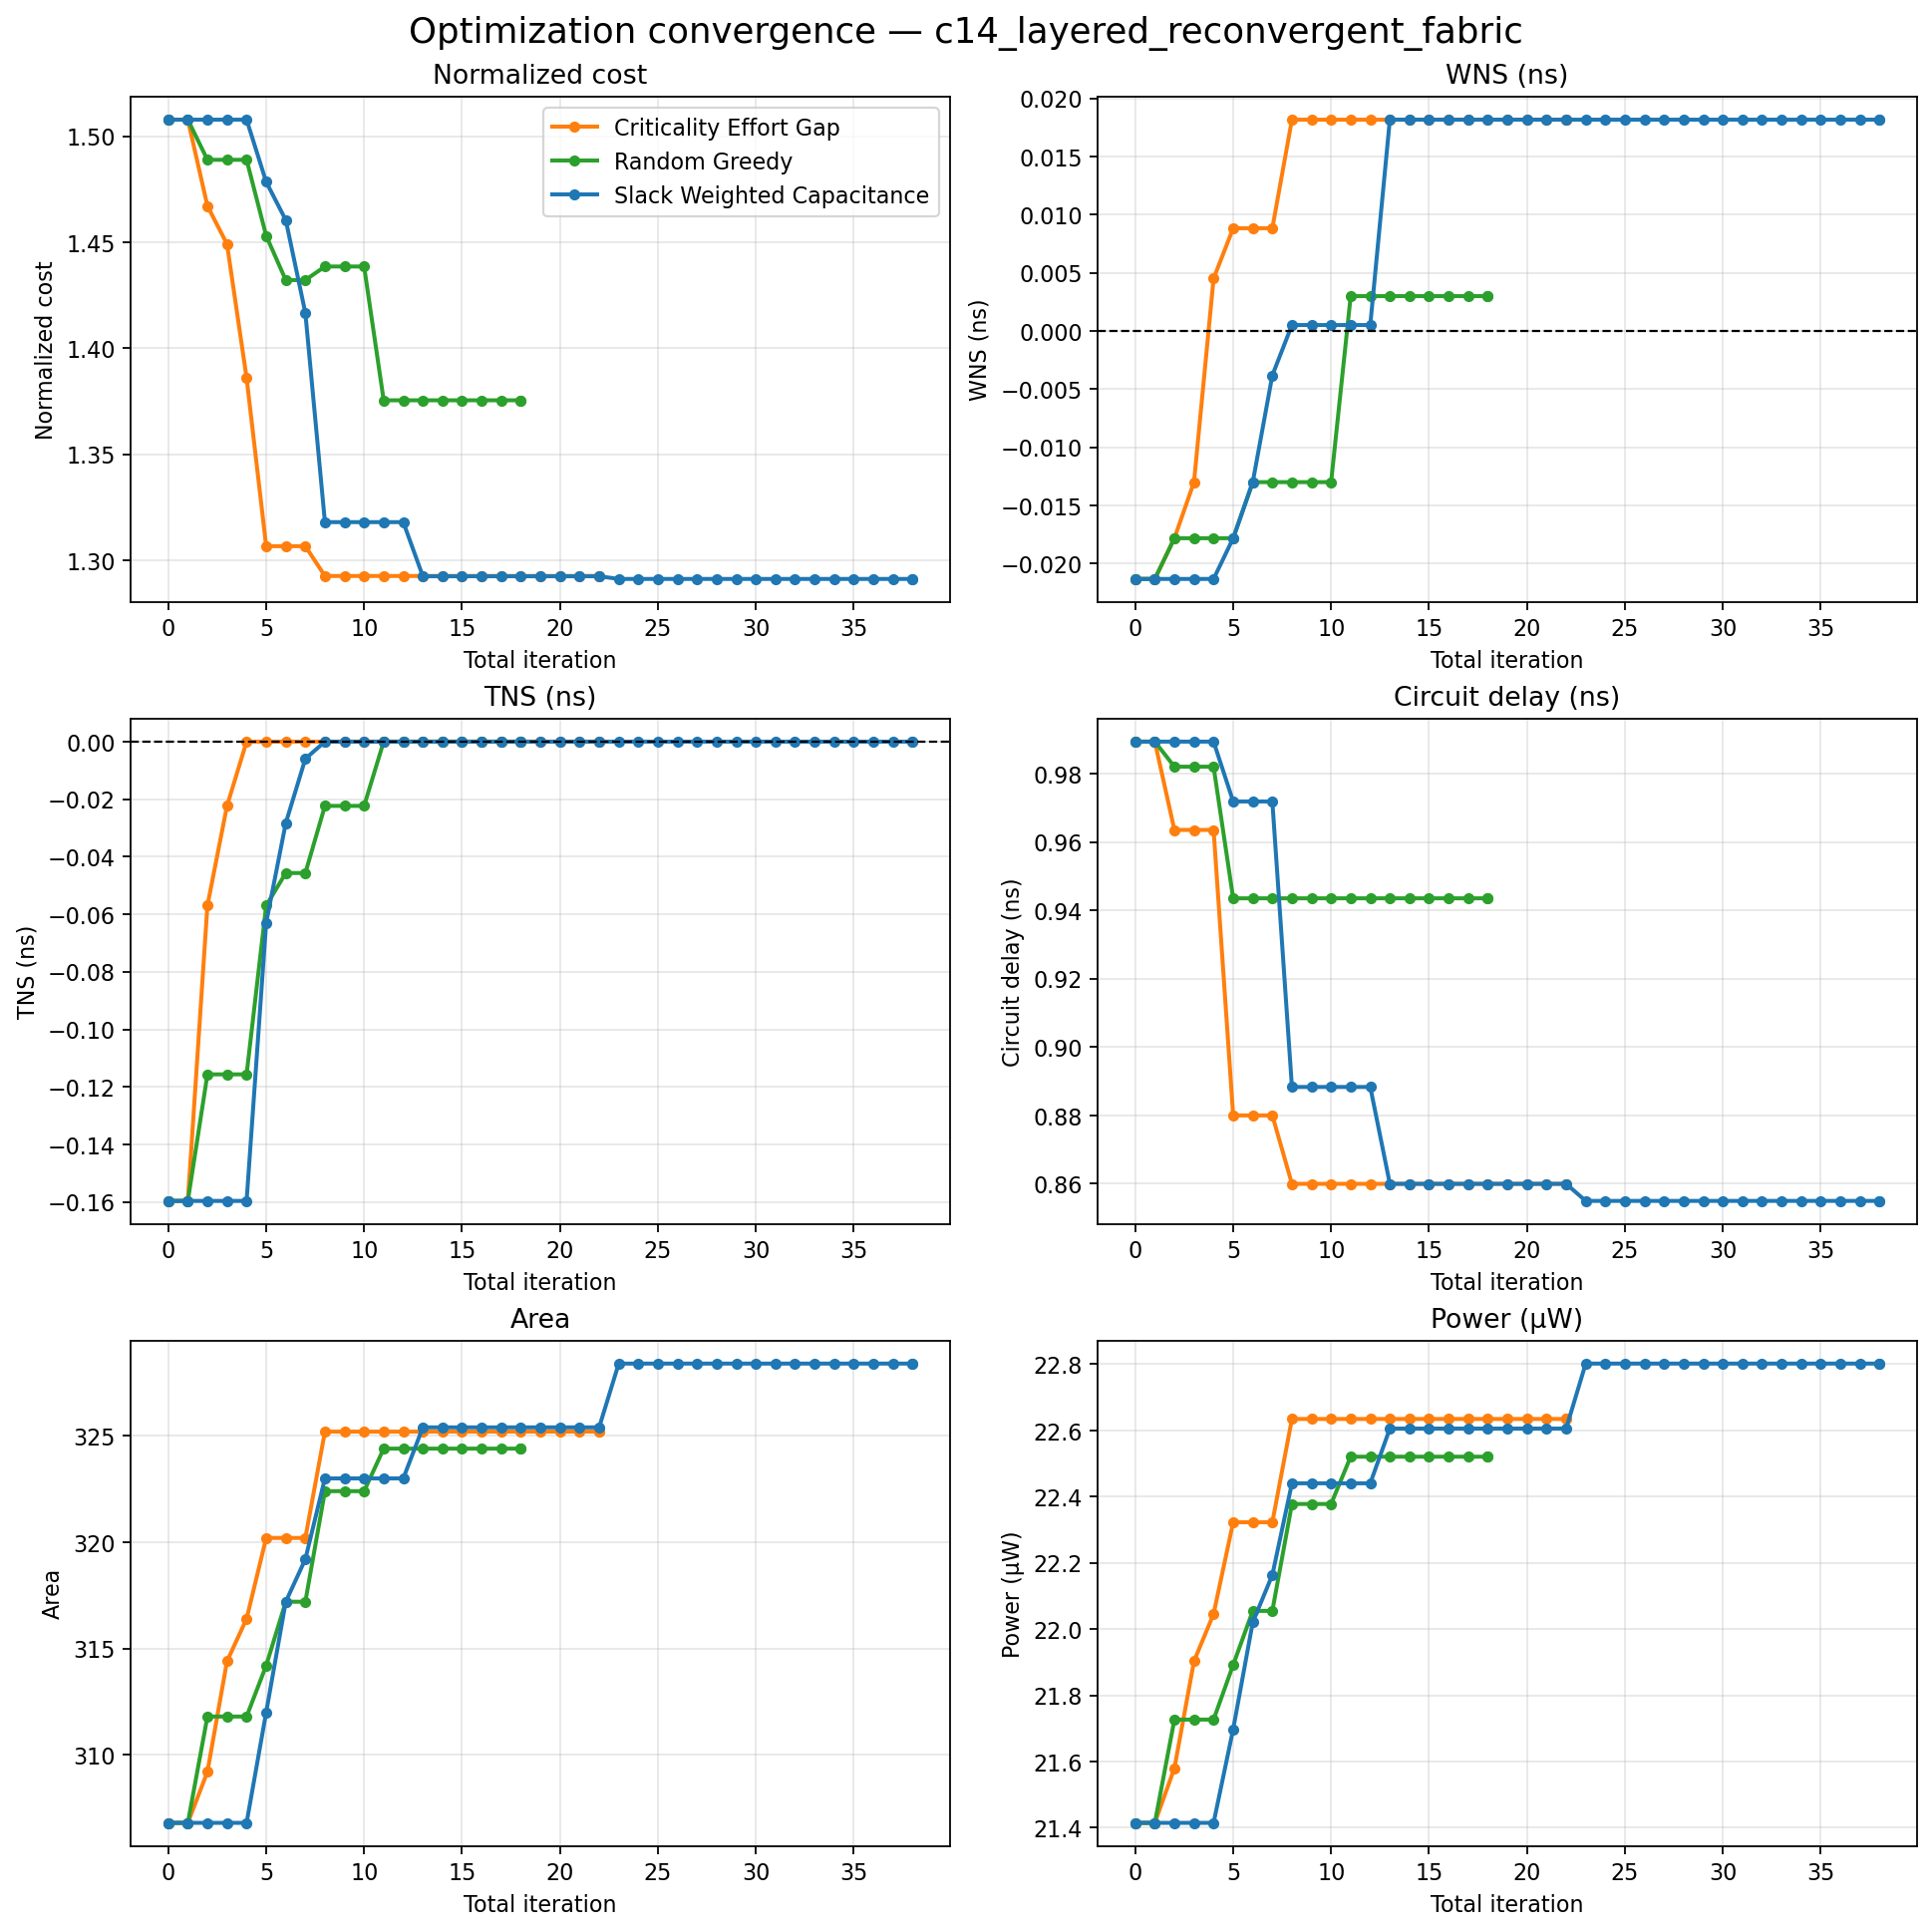
\includegraphics[width=\textwidth]{c14_layered_reconvergent_fabric_conv.png}
    \caption{\texttt{c14\_layered\_reconvergent\_fabric}: optimization convergence trace.}
    \label{fig:app-c14-layered-reconvergent-fabric-conv}
\end{figure}

\begin{figure}[H]
    \centering
    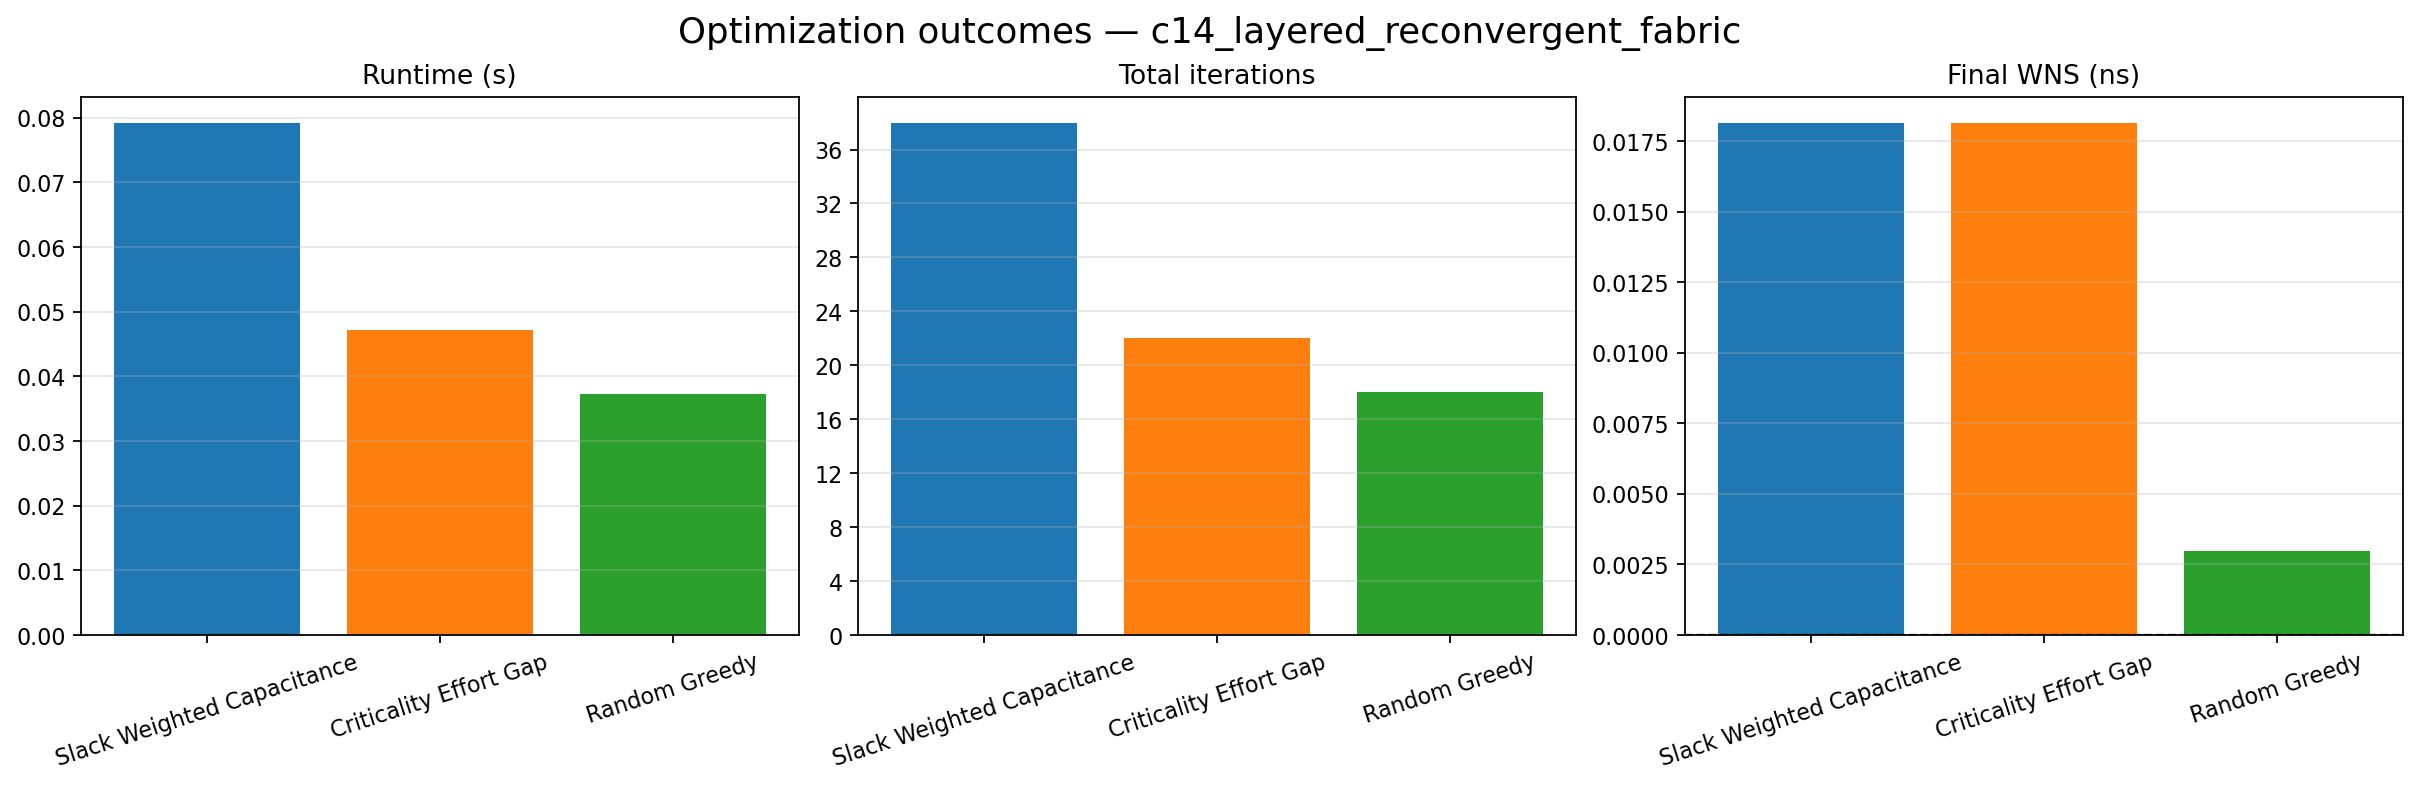
\includegraphics[width=\textwidth]{c14_layered_reconvergent_fabric_outc.png}
    \caption{\texttt{c14\_layered\_reconvergent\_fabric}: optimization outcomes summary.}
    \label{fig:app-c14-layered-reconvergent-fabric-outc}
\end{figure}

\clearpage

\section{\texttt{c15\_high\_fanout\_sizing\_fabric} (118 gates)}
\label{app:fig-c15-high-fanout-sizing-fabric}

\begin{figure}[H]
    \centering
    \begin{subfigure}[t]{0.48\textwidth}
        \centering
        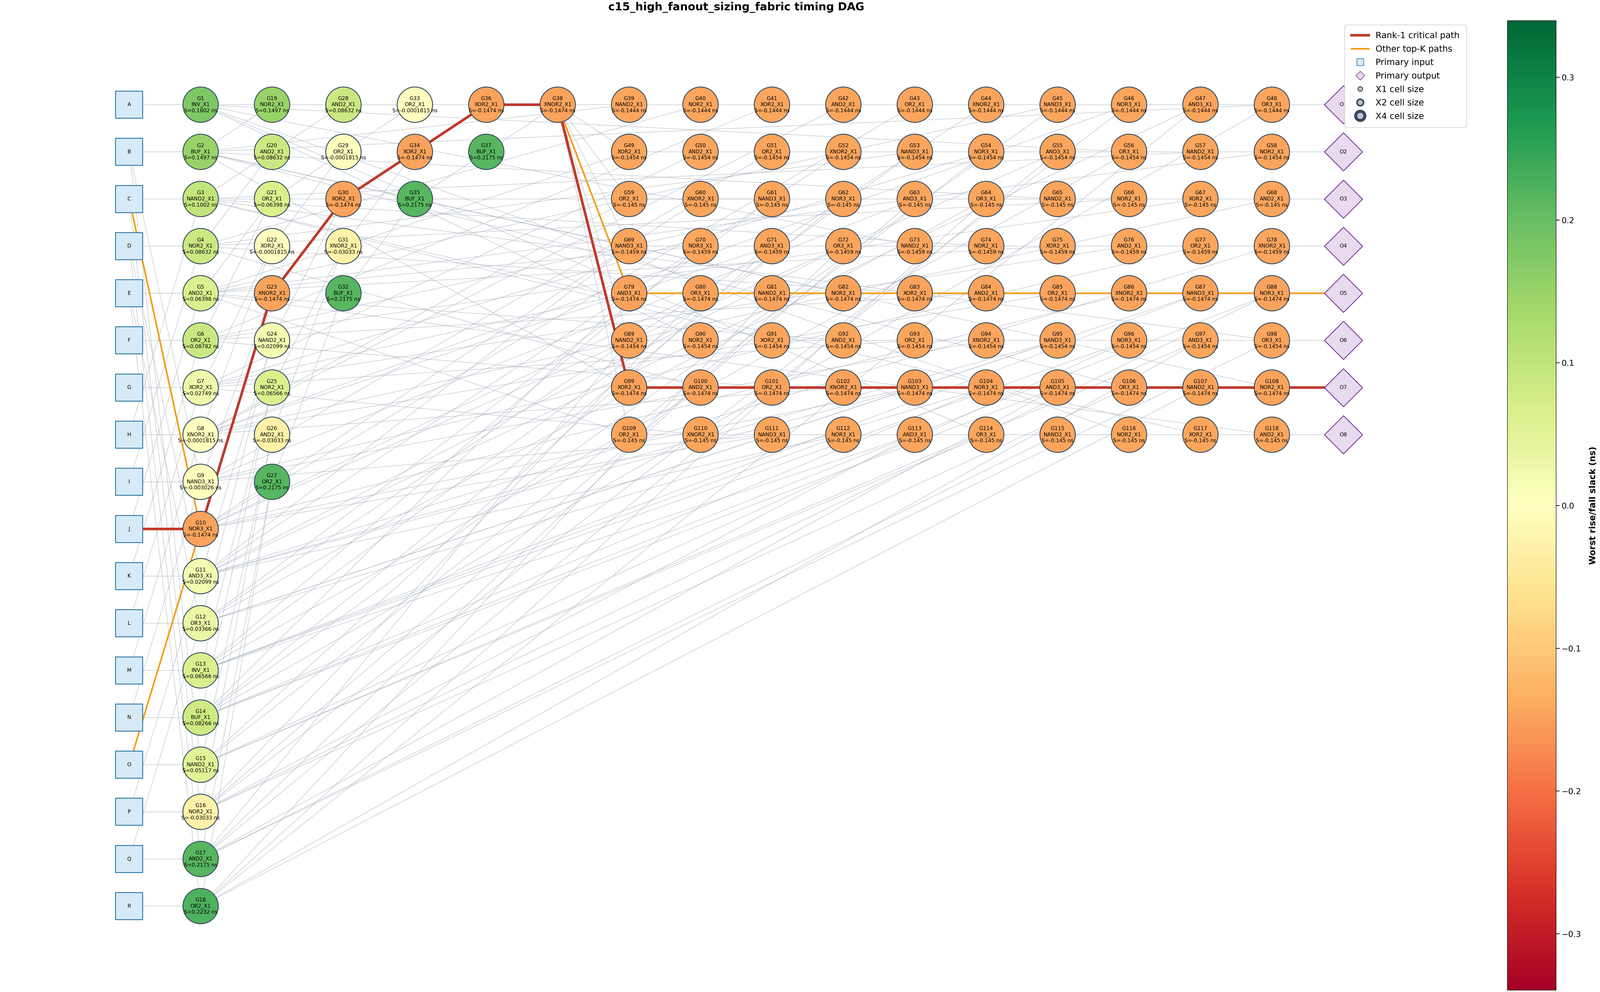
\includegraphics[width=\textwidth]{c15_high_fanout_sizing_fabric_pre.png}
        \caption{Pre-optimization}
    \end{subfigure}
    \hfill
    \begin{subfigure}[t]{0.48\textwidth}
        \centering
        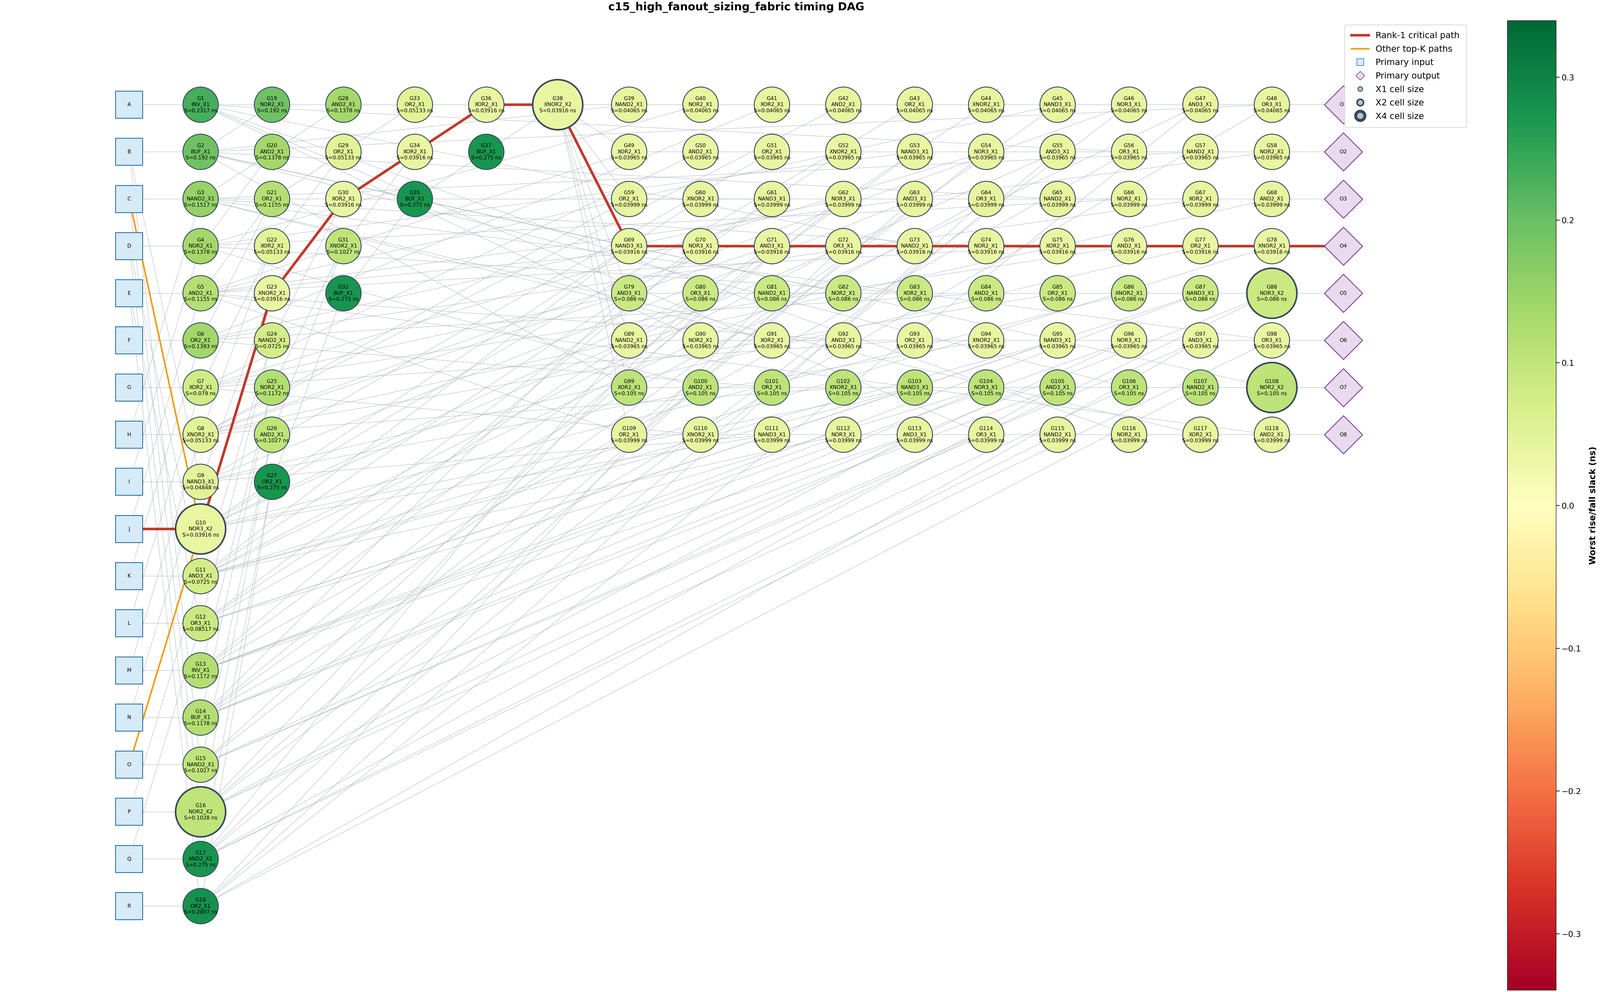
\includegraphics[width=\textwidth]{c15_high_fanout_sizing_fabric_post.png}
        \caption{Post-optimization}
    \end{subfigure}
    \caption{\texttt{c15\_high\_fanout\_sizing\_fabric}: circuit diagrams, nodes colored by slack,
    critical path highlighted.}
    \label{fig:app-c15-high-fanout-sizing-fabric-graphs}
\end{figure}

\begin{figure}[H]
    \centering
    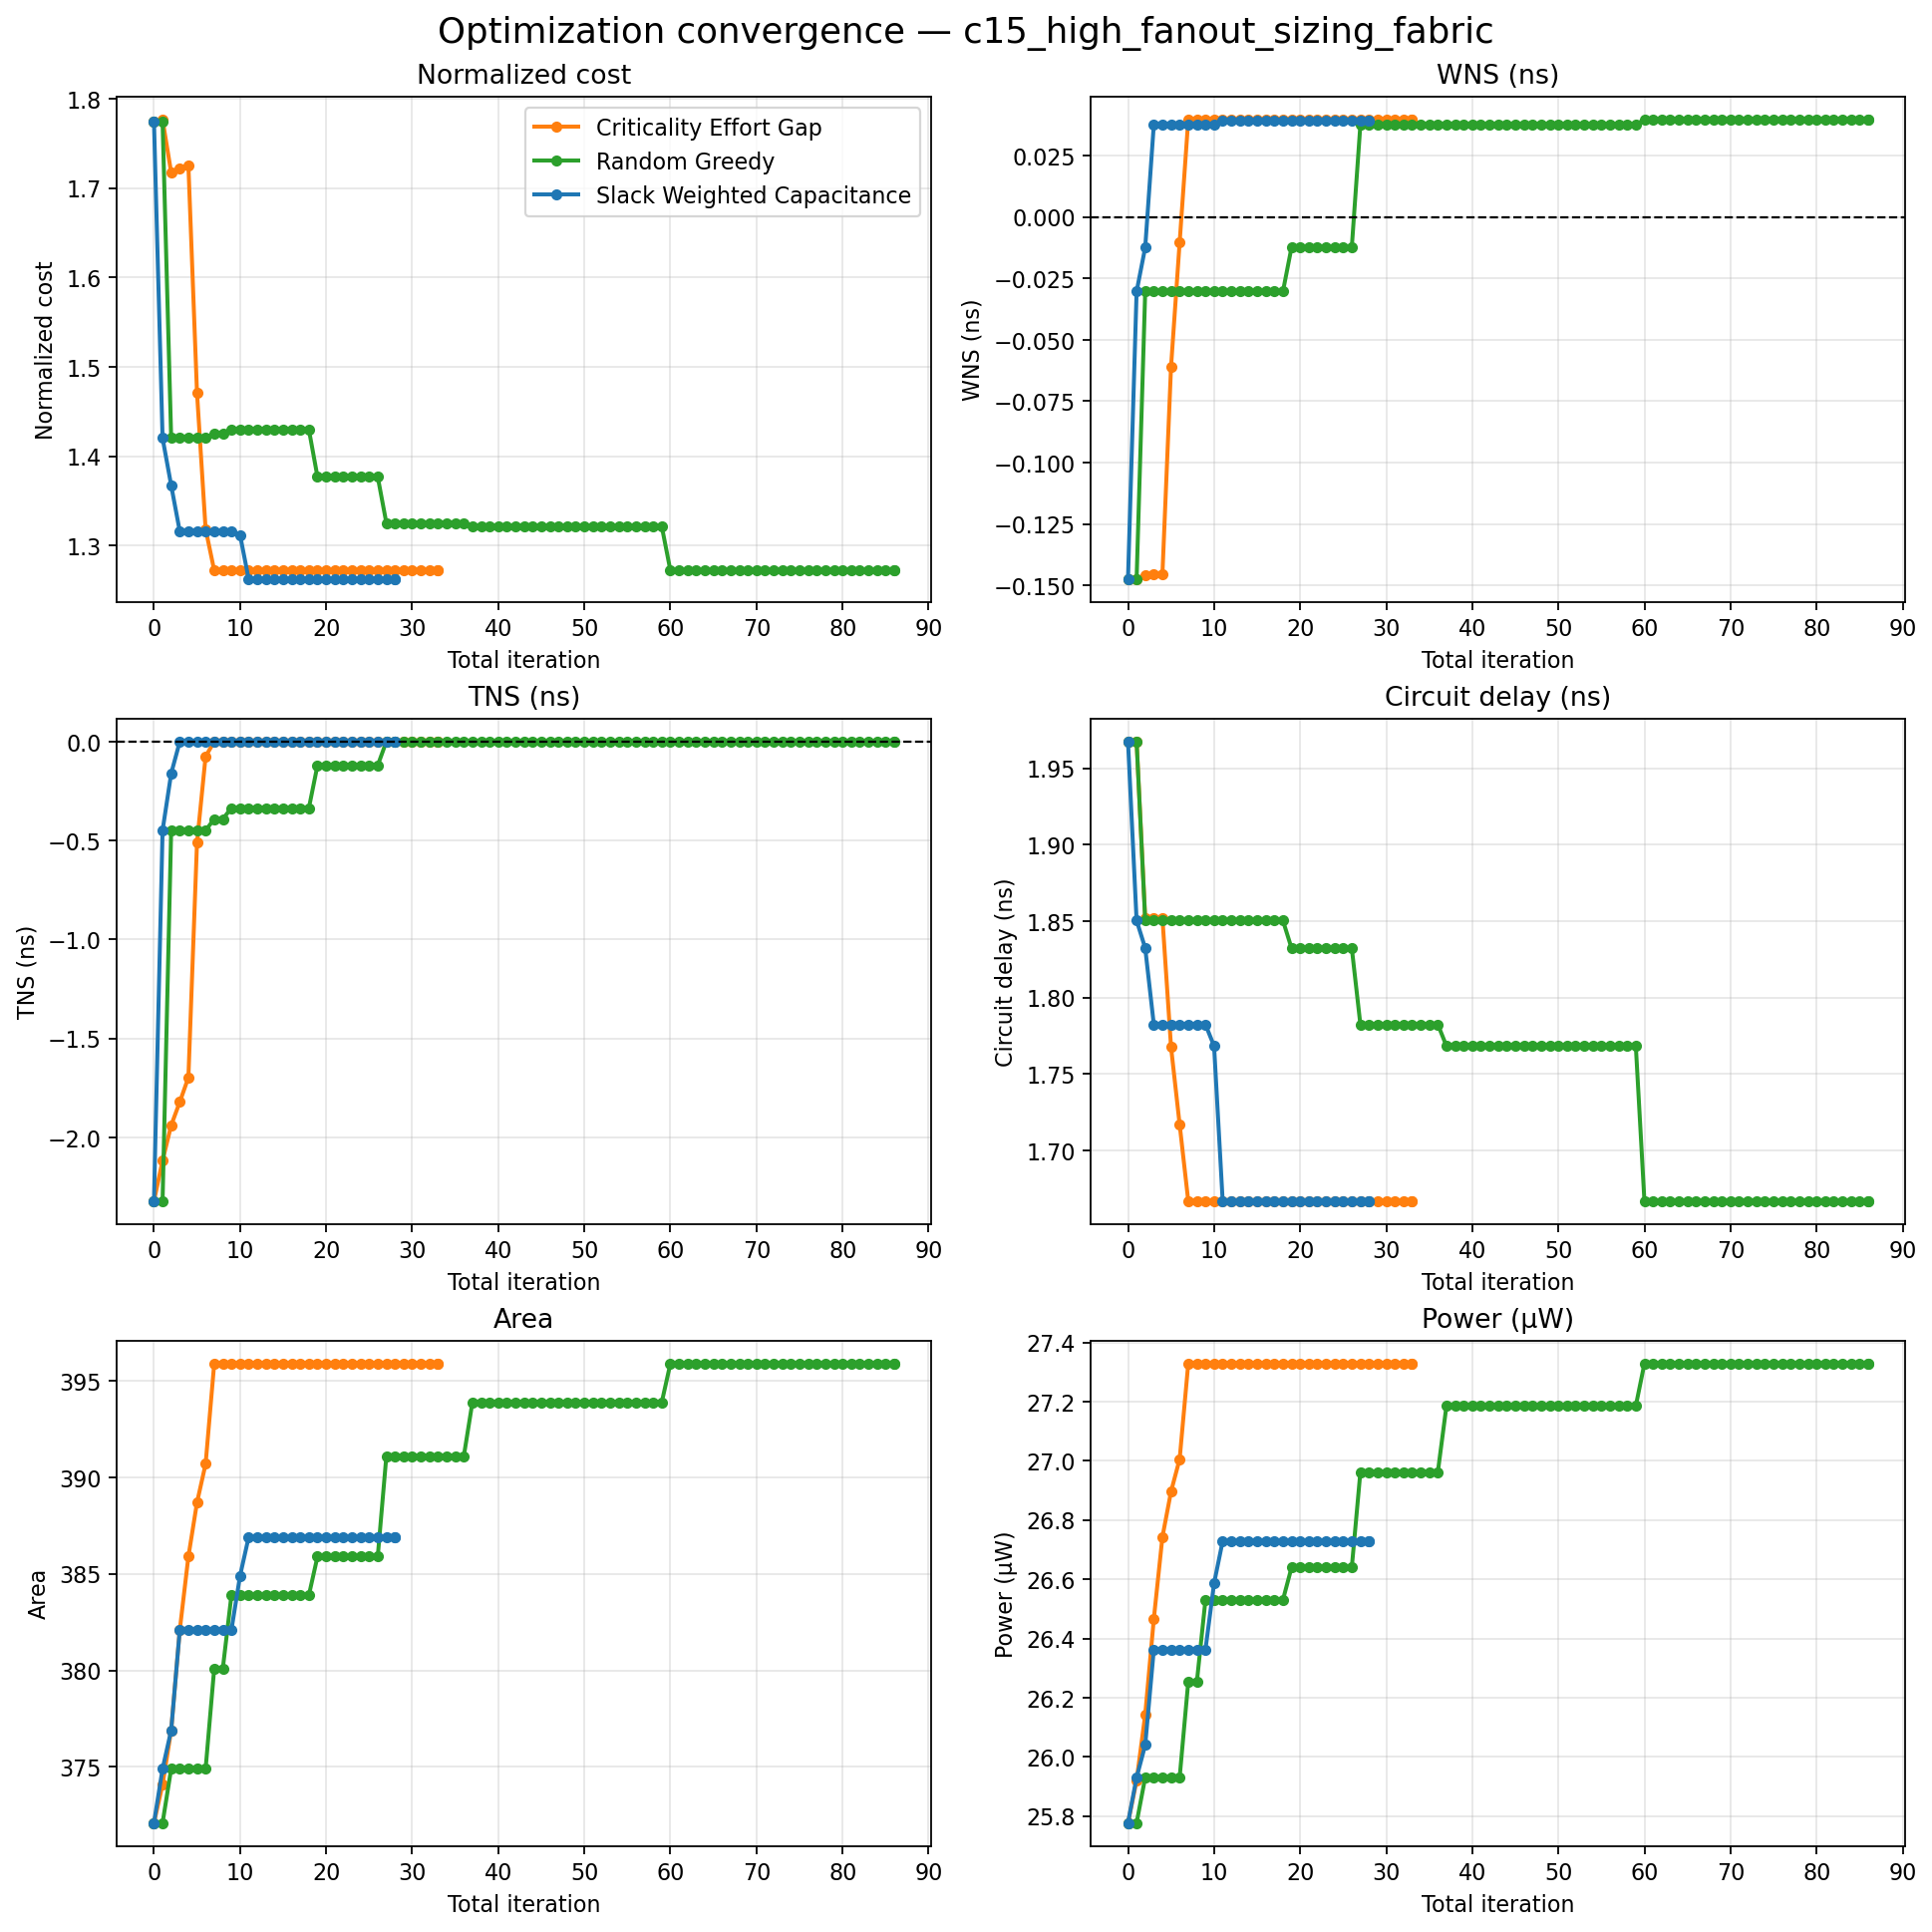
\includegraphics[width=\textwidth]{c15_high_fanout_sizing_fabric_conv.png}
    \caption{\texttt{c15\_high\_fanout\_sizing\_fabric}: optimization convergence trace.}
    \label{fig:app-c15-high-fanout-sizing-fabric-conv}
\end{figure}

\begin{figure}[H]
    \centering
    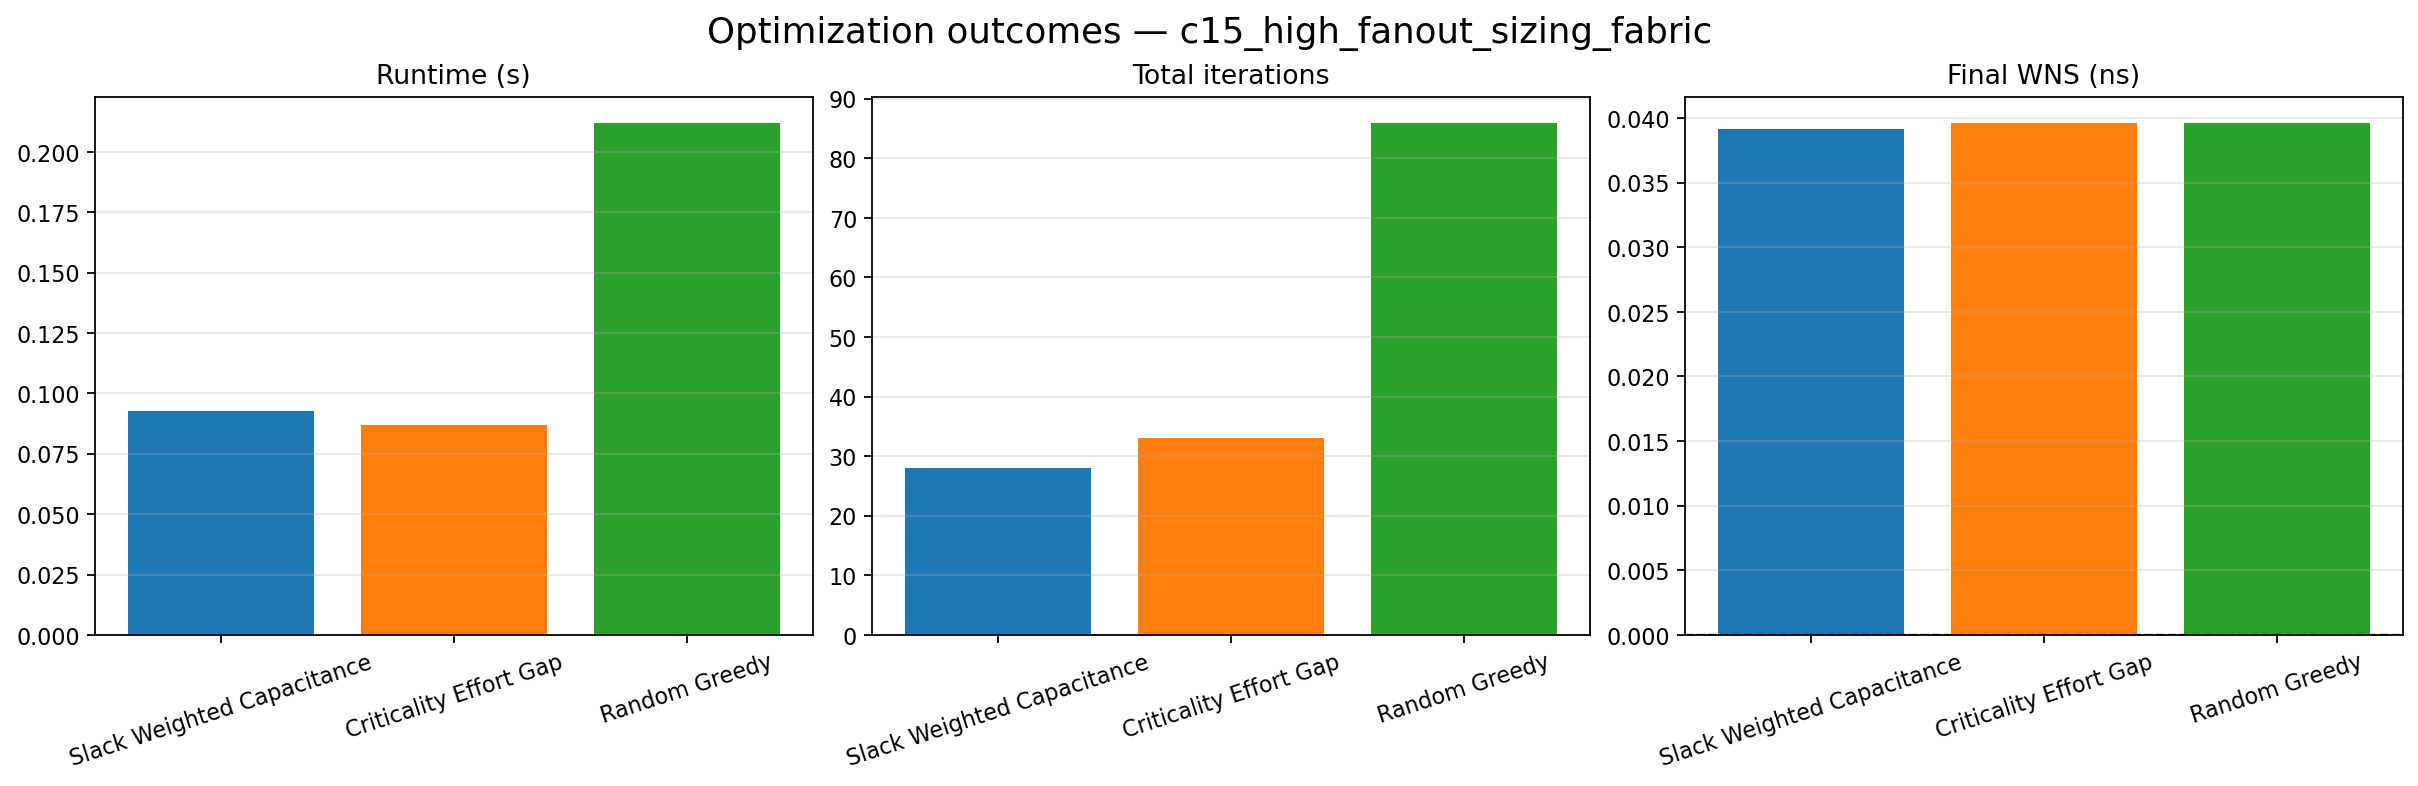
\includegraphics[width=\textwidth]{c15_high_fanout_sizing_fabric_outc.png}
    \caption{\texttt{c15\_high\_fanout\_sizing\_fabric}: optimization outcomes summary.}
    \label{fig:app-c15-high-fanout-sizing-fabric-outc}
\end{figure}

\clearpage


\end{appendices}


% \clearpage
% \begin{thebibliography}{9}
% \bibitem{sutherland1999logical}
% I.~Sutherland, B.~Sproull, and D.~Harris,
% \emph{Logical Effort: Designing Fast CMOS Circuits}.
% San Francisco, CA: Morgan Kaufmann Publishers, 1999.

% \bibitem{assignment2026}
% S.~Hesabi, \emph{Advanced VLSI Design --- Course Project: Static Timing
% Analysis and Gate Sizing}, Department of Computer Engineering course
% handout, Semester 2, 1404--1405.
% \end{thebibliography}
% \addcontentsline{toc}{chapter}{Bibliography}

\end{document}